\PassOptionsToPackage{unicode=true}{hyperref} % options for packages loaded elsewhere
\PassOptionsToPackage{hyphens}{url}
%
\documentclass[]{book}
\usepackage{lmodern}
\usepackage{amssymb,amsmath}
\usepackage{ifxetex,ifluatex}
\usepackage{fixltx2e} % provides \textsubscript
\ifnum 0\ifxetex 1\fi\ifluatex 1\fi=0 % if pdftex
  \usepackage[T1]{fontenc}
  \usepackage[utf8]{inputenc}
  \usepackage{textcomp} % provides euro and other symbols
\else % if luatex or xelatex
  \usepackage{unicode-math}
  \defaultfontfeatures{Ligatures=TeX,Scale=MatchLowercase}
\fi
% use upquote if available, for straight quotes in verbatim environments
\IfFileExists{upquote.sty}{\usepackage{upquote}}{}
% use microtype if available
\IfFileExists{microtype.sty}{%
\usepackage[]{microtype}
\UseMicrotypeSet[protrusion]{basicmath} % disable protrusion for tt fonts
}{}
\IfFileExists{parskip.sty}{%
\usepackage{parskip}
}{% else
\setlength{\parindent}{0pt}
\setlength{\parskip}{6pt plus 2pt minus 1pt}
}
\usepackage{hyperref}
\hypersetup{
            pdftitle={环境黑板报},
            pdfauthor={805},
            pdfborder={0 0 0},
            breaklinks=true}
\urlstyle{same}  % don't use monospace font for urls
\usepackage{longtable,booktabs}
% Fix footnotes in tables (requires footnote package)
\IfFileExists{footnote.sty}{\usepackage{footnote}\makesavenoteenv{longtable}}{}
\usepackage{graphicx,grffile}
\makeatletter
\def\maxwidth{\ifdim\Gin@nat@width>\linewidth\linewidth\else\Gin@nat@width\fi}
\def\maxheight{\ifdim\Gin@nat@height>\textheight\textheight\else\Gin@nat@height\fi}
\makeatother
% Scale images if necessary, so that they will not overflow the page
% margins by default, and it is still possible to overwrite the defaults
% using explicit options in \includegraphics[width, height, ...]{}
\setkeys{Gin}{width=\maxwidth,height=\maxheight,keepaspectratio}
\setlength{\emergencystretch}{3em}  % prevent overfull lines
\providecommand{\tightlist}{%
  \setlength{\itemsep}{0pt}\setlength{\parskip}{0pt}}
\setcounter{secnumdepth}{5}
% Redefines (sub)paragraphs to behave more like sections
\ifx\paragraph\undefined\else
\let\oldparagraph\paragraph
\renewcommand{\paragraph}[1]{\oldparagraph{#1}\mbox{}}
\fi
\ifx\subparagraph\undefined\else
\let\oldsubparagraph\subparagraph
\renewcommand{\subparagraph}[1]{\oldsubparagraph{#1}\mbox{}}
\fi

% set default figure placement to htbp
\makeatletter
\def\fps@figure{htbp}
\makeatother

\usepackage{booktabs}
\usepackage{ctex}
\setCJKmainfont{STFangsong}
\setCJKmonofont{STKaiti}
\setCJKsansfont{STHeiti}
\renewcommand{\chaptername}{章}
\usepackage[]{natbib}
\bibliographystyle{plainnat}

\title{环境黑板报}
\author{805}
\date{2020-01-02}

\begin{document}
\maketitle

{
\setcounter{tocdepth}{1}
\tableofcontents
}
\hypertarget{ux524dux8a00}{%
\chapter{前言}\label{ux524dux8a00}}

环境黑板报的文章存档

\begin{itemize}
\item
  研究速递(研究动态、政策速递等)
\item
  科普讲堂(基础研究类、知识类科普等)
\item
  工程实践(实用技术、应用技术介绍等)
\item
  科苑风采(个人感悟、工作随笔、风采展示)
\item
  就业咨询(环境类就业方向研讨)
\end{itemize}

\hypertarget{ux524dux6cbfux8d44ux8baf}{%
\chapter{前沿资讯}\label{ux524dux6cbfux8d44ux8baf}}

\hypertarget{ux5341ux4e00ux6708}{%
\section*{十一月}\label{ux5341ux4e00ux6708}}
\addcontentsline{toc}{section}{十一月}

\hypertarget{ux7814ux7a76ux52a8ux6001}{%
\subsection*{研究动态}\label{ux7814ux7a76ux52a8ux6001}}
\addcontentsline{toc}{subsection}{研究动态}

本栏目旨在介绍环境科学、环境工程与生态学及相关学科近期发表的有意思的研究

\begin{itemize}
\tightlist
\item
  海洋微塑料正在成为研究热点,但密歇根大学的 Allen Burton 却在ES\&T上发了篇 Viewpoint 泼冷水,在他眼里,这类研究缺少风险评价,可能毫无意义
\end{itemize}

推荐人:田振宇

文献链接 \url{http://pubs.acs.org/doi/10.1021/acs.est.7b05463}

\begin{itemize}
\tightlist
\item
  谷歌正在用车载传感器检测街道级别的空气质量
\end{itemize}

推荐人:于淼

文献链接 \url{http://flowingdata.com/2017/11/08/google-maps-street-level-air-quality-using-street-view-cars-with-sensors/}

\begin{itemize}
\tightlist
\item
  城市热岛效应所引发的温度跟相对湿度变化会影响半挥发化合物的溶解度进而影响pH值,研究人员发现巴尔的摩市跟芝加哥城市跟郊区上空的pH差异在0.8与0.65,当我们讨论区域尺度的大气污染时,城乡差异的来源可能比想象的要复杂
\end{itemize}

推荐人:于淼

文献链接 \url{http://pubs.acs.org/doi/10.1021/acs.est.7b02786}

\begin{itemize}
\tightlist
\item
  科研作图是很多研究生痛苦的一个根源,然而并不是越炫酷越好,下面这个例子可以说是一个反面教材,过多的立体化、文字化与阴影化处理丢失了图片传达信息的意图,不如直接用表格 (编自 Andrew Gelman的博客)
\end{itemize}

推荐人:于淼

链接 \url{https://www.memphisflyer.com/NewsBlog/archives/2016/08/26/report-alcohol-crashes-down-distracted-driving-accidents-up}

\hypertarget{ux7814ux7a76ux7b80ux62a5}{%
\subsection*{805研究简报}\label{ux7814ux7a76ux7b80ux62a5}}
\addcontentsline{toc}{subsection}{805研究简报}

本栏目旨在介绍805班同学发表的论文

\hypertarget{ux83ccux6839ux8010ux94ecux673aux7406ux83b7ux65b0ux8fdbux5c55---ux4f0dux677eux6797}{%
\subsubsection*{菌根耐铬机理获新进展 - 伍松林}\label{ux83ccux6839ux8010ux94ecux673aux7406ux83b7ux65b0ux8fdbux5c55---ux4f0dux677eux6797}}
\addcontentsline{toc}{subsubsection}{菌根耐铬机理获新进展 - 伍松林}

做为陆地上最为广泛的微生物之一,丛枝菌根(arbuscular mycorrhiza, AM)真菌能与绝大多数的陆地高等植物形成共生体系,帮助植物适应养分贫瘠、干旱、重金属污染等各种逆境胁迫。AM真菌在植物耐受铬污染胁迫中具有重要作用,因而在铬污染土壤生态恢复中具有极大潜在应用价值。然而AM如何促进植物耐受铬污染尚不得而知。

最近一项研究表明AM真菌在六价铬污染情况下能够上调植物根系高亲和硫酸根转运蛋白基因的表达,促进植物根系对硫的吸收。AM真菌同时系统调控了硫在植物体内的转运和代谢以抵御铬污染胁迫。硫代谢产物如半胱氨酸(cysteine, Cys), 谷胱甘肽(glutathione, GSH), 植物络合素(phytochelatins, PCs)等往往能够通过巯基与金属阳离子相结合,进而降低金属毒性。基于此,研究人员推断,AM根系中应有更多的铬与巯基相结合。

然而,事实并非如此,基于同步辐射光源的XAFS分析技术发现,相比较未接种根系,接种AM真菌的根系中有较少的铬与巯基相结合,相反,磷酸结合态铬在AM根系中占主导。这似乎说明,硫代谢产物在菌根耐铬中的作用并不在于络合金属铬。有趣的是,研究人员通过相关分析初步发现,这些主要硫代谢产物(Cys, GSH, PCs)可能在缓解铬引起的植物氧化胁迫中起着重要作用。

相关文章参见:\url{https://www.sciencedirect.com/science/article/pii/S0098847217302939}

\hypertarget{ux5341ux4e8cux6708}{%
\section*{十二月}\label{ux5341ux4e8cux6708}}
\addcontentsline{toc}{section}{十二月}

\hypertarget{ux7814ux7a76ux52a8ux6001-1}{%
\subsection*{研究动态}\label{ux7814ux7a76ux52a8ux6001-1}}
\addcontentsline{toc}{subsection}{研究动态}

\begin{itemize}
\tightlist
\item
  辣木籽被国内保健行业广为吹捧,但它其实是水处理界的明星,将其混合沙子作为滤水器可以去除99\%的颗粒物与细菌
\end{itemize}

推荐人:于淼

链接:\url{http://pubs.acs.org/doi/10.1021/acs.estlett.7b00490}

\begin{itemize}
\tightlist
\item
  这篇等了很久了,USEPA对家用净水器滤芯做的嫌疑物筛选分析和非目标分析。所采用的Brita Filter是美国最常见的家用简易净水器,滤芯里是活性炭和阳离子交换树脂(他们应该给我广告费啊)。饮用水里有哪些污染物?看看这篇文章吧!
\end{itemize}

非常不错的一个暴露组学范例研究,用非目的分析配合数据库筛选环境水样中的毒性化合物,目测重复难度不大,不过完成这个实验需要多领域专家协作,这篇是EPA外带橡树岭国家实验室配合出来的,国内有同等战力的单位屈指可数

推荐人:田振宇、于淼

链接:\url{https://www.sciencedirect.com/science/article/pii/S026974911732691X}

\begin{itemize}
\tightlist
\item
  把汽车型号,费用,和减排目标联系起来做分析,看看什么车既便宜又环保(可是一般电动车不好修而且开起来太肉啊,well,作者是不是收了Tesla钱了 (●′ω`●))
\end{itemize}

推荐人:田振宇

链接:\url{http://pubs.acs.org/doi/10.1021/acs.est.6b00177}

\begin{itemize}
\tightlist
\item
  毒理学研究往往考察单一污染物对单一毒性的影响,EHP上的评论文章引用了一篇双酚类污染物复合暴露的研究指出,针对多污染物与多毒性终点的研究可能给出更多毒理学信息,也需要新的方法学创新
\end{itemize}

推荐人:于淼

链接:\url{https://ehp.niehs.nih.gov/ehp2341/} \url{https://ehp.niehs.nih.gov/ehp2325}

\begin{itemize}
\tightlist
\item
  Environmental DNA (eDNA) 是近些年提出的新概念,指环境样品中可直接测定的非生物来源DNA,可定量分析环境多样性变化,我很好奇这是不是那些搞基因组的发现自己技术过时了就包装下输送到考古跟环境研究领域抢经费了,不过确实是个不错的指标,有希望成为研究热点
\end{itemize}

推荐人:于淼

链接:\url{http://pubs.acs.org/doi/10.1021/acs.est.7b05199} \url{http://www.sciencedirect.com/science/article/pii/S0006320714004443}

\begin{itemize}
\tightlist
\item
  Scripps研究所一直是化学类研究的前沿阵地,脑洞也比较大,在近期提出的一套暴露组学研究流程中研究人员使用了IBM的Watson AI系统来学习文献中的分子并评价暴露组学筛选出的分子,这是要让多少人丢饭碗啊
\end{itemize}

推荐人:于淼

链接:\url{http://pubs.acs.org/doi/full/10.1021/acs.analchem.7b02759}

\begin{itemize}
\tightlist
\item
  ``赏金科学家''召集令!!!美国农垦总局出价十万美金征集根除水体中斑马贻贝的方案,欢迎物种入侵相关研究组来美捞金,毕竟一个方案就是两个面上的钱,截止日期二月底
\end{itemize}

推荐人:于淼

链接:\url{https://www.innocentive.com/ar/workspace/challengeDetail?challenge=9933880}

\begin{itemize}
\tightlist
\item
  来自中国的研究组测了下海盐、湖盐和井盐中的塑料纤维,发现海盐里微塑料明显多于井盐,这个视角比较独特,直接跟食品挂钩了,不过依然缺少风险评价
\end{itemize}

推荐人:于淼

链接:\url{http://pubs.acs.org/doi/10.1021/acs.est.5b03163}

\begin{itemize}
\tightlist
\item
  这个有点像淼哥之前推荐的 Environmental DNA (eDNA) 那个,不同的是研究者着眼于抗生素抗性基因(antibiotic resistance genes, ARG, 也就是耐药超级细菌所需要的基因)。在污水处理过程中细胞相关的ARG能被较为高效地清除,但是游离的胞外ARG去除效率较低,可能是耐药基因的一个重要来源
\end{itemize}

推荐人:田振宇

链接:\url{http://pubs.acs.org/doi/10.1021/acs.est.7b04283}

\begin{itemize}
\tightlist
\item
  原来以为原生动物除了难杀灭和能引起奇怪的病之外就没啥意义。然而最近EAWAG的一项研究发现,活性污泥中的原生动物能够通过电荷吸附的作用去除污水中的胺类。
\end{itemize}

推荐人:田振宇

链接:\url{http://pubs.acs.org/doi/10.1021/acs.est.7b03556}

\begin{itemize}
\tightlist
\item
  五大湖的藻华会影响类似海盐气溶胶的淡水湖气溶胶,单颗粒质谱技术或气溶胶质谱技术有助于我们研究这一特定环境过程,这类概念很不错,但落地还是需要未知物鉴定的数据分析技术,不然还是pca游戏
\end{itemize}

推荐人:于淼

链接:\url{http://pubs.acs.org/doi/10.1021/acs.est.7b03609}

\begin{itemize}
\tightlist
\item
  拿NHANES数据集发ES\&T不新鲜,但搞个10年前的ANN算法来溯源就有点过分了,这种题目放到数据类MOOCs上当作业可能都是送分题,而且数据质量也太差了,0.3\%到0.5\%的灵敏度还不如随机噪音,没有验证集结果根本就是瞎猜
\end{itemize}

推荐人:于淼

链接:\url{http://pubs.acs.org/doi/10.1021/acs.est.7b05128}

\hypertarget{ux7814ux7a76ux7b80ux62a5-1}{%
\subsection*{805研究简报}\label{ux7814ux7a76ux7b80ux62a5-1}}
\addcontentsline{toc}{subsection}{805研究简报}

本栏目旨在介绍805班同学发表的论文

\hypertarget{ux6c2eux6742ux73afux82b3ux70c3ux73afux5883ux8fc7ux7a0bux7814ux7a76ux65b0ux8fdbux5c55---ux7530ux632fux5b87}{%
\subsubsection*{氮杂环芳烃环境过程研究新进展 - 田振宇}\label{ux6c2eux6742ux73afux82b3ux70c3ux73afux5883ux8fc7ux7a0bux7814ux7a76ux65b0ux8fdbux5c55---ux7530ux632fux5b87}}
\addcontentsline{toc}{subsubsection}{氮杂环芳烃环境过程研究新进展 - 田振宇}

氮杂环芳烃(azaarenes)是多环芳烃(PAHs)的氮取代类似物。这类污染物常伴随多环芳烃同时出现在污染场地中,但是由于分析方法的限制,目前对于它们的浓度和环境行为了解十分有限。特别是已知具有较强毒性的高分子量(4-5环)氮杂环芳烃,在各种环境介质的信息都比较缺乏。现有研究大多集中于低分子量(2-3环)的少数几个同类物。换句话说,这类污染物中最危险的东西,我们了解的最少,需要填补这一信息上的空白。

基于高分辨质谱(HRMS)和质量亏损过滤(mass defect filtering),本研究将一种非目标分析方法应用于四个不同污染场地的土壤样品,检测出8个系列共232个同类物。其中四环和五环的氮杂环芳烃被大量检出,种类和浓度都较高。对比污染场地中污染物的分布,可见风化程度高的土壤中四环和五环氮杂环芳烃比例更高。已知有毒且有致癌性的的benzo{[}c{]}acridine和dibenzo{[}a,h{]}acridine被检出,并且发现它们具有较多的同分异构体。
从本研究可以得出的主要结论是:

\begin{itemize}
\item
  由于以往的研究忽略了氮杂环芳烃的多样性,它们在污染土壤的毒性中起到的作用很可能被低估;
\item
  对于土壤中氮杂环芳烃的研究,应更多集中于以往较少关注的高分子量同类物,因为它们的浓度较高且具有持久性。
\end{itemize}

链接:\url{http://pubs.acs.org/doi/abs/10.1021/acs.est.7b03319}
(其实窝是810班的)

\hypertarget{ux4e00ux6708}{%
\section*{一月}\label{ux4e00ux6708}}
\addcontentsline{toc}{section}{一月}

\hypertarget{ux7814ux7a76ux52a8ux6001-2}{%
\subsection*{研究动态}\label{ux7814ux7a76ux52a8ux6001-2}}
\addcontentsline{toc}{subsection}{研究动态}

\begin{itemize}
\tightlist
\item
  ES\&T Letter 的执行主编是一个特别喜欢写 editorial 的教授,哪怕一期就三四篇,在 Letter 的 IF 没有超过正刊后,主编大人自己定义了一个 Author Impact Factor(AIF),用过去两年发表数除以2,然后又定义了 L 因子(用 AIF 除以发表期刊的平均 IF ),不得不说这个指标就比较难刷了,有一点他说的非常在理,期刊要以发表的工作为荣,而不是反过来。
\end{itemize}

推荐人:于淼

链接:\url{http://pubs.acs.org/doi/10.1021/acs.estlett.7b00546}

\begin{itemize}
\tightlist
\item
  用高通量metagenomics 测室内空气中的病毒核酸,采样的地方是12个大学宿舍。宿主多样性很高,而且病毒群落组成可能反映与房间居住者的关联。
\end{itemize}

推荐人:田振宇

链接:\url{http://pubs.acs.org/doi/10.1021/acs.est.7b04203}

\begin{itemize}
\tightlist
\item
  考虑停留时间,室内空气污染其实比室外影响要大,清华大学的一个研究组考察了中式烹饪过程中室内污染的影响因素,结果发现烹饪方式对大多数污染物影响最严重,基本趋势是炒菜\textgreater{}油炸\textgreater{}蒸煮,如果开了排气扇,大多数污染物浓度都能下降一半。
\end{itemize}

推荐人:于淼

链接:\url{http://pubs.acs.org/doi/10.1021/acs.est.7b05600}

\begin{itemize}
\tightlist
\item
  左旋葡聚糖经常被用来作为生物质燃烧的标志污染物进行溯源,然而最近的研究发现燃煤也可以生成左旋葡聚糖,这导致我们可能高估了北京的细颗粒物中生物质燃烧的贡献,特别是有燃煤行为的地区
\end{itemize}

推荐人:于淼

链接:\url{http://pubs.acs.org/doi/10.1021/acs.est.7b05858}

\begin{itemize}
\tightlist
\item
  关于精子质量和大气颗粒物之间关联的流行病学研究。结论比较有意思,说 PM10 (以及与 PM2.5的差) 与精子质量有负相关性,而不是PM2.5。但是大气颗粒物的数据来自区域性的监测和调查问卷,感觉不是很靠谱。
\end{itemize}

推荐人:田振宇

链接:\url{http://pubs.acs.org/doi/10.1021/acs.est.7b05206}

\begin{itemize}
\tightlist
\item
  光化学反应能在道路尘土中产生单线态氧。大气气相反应和水体光化学反应中的单线态氧并不稀奇,考虑到颗粒物本身就带有各种污染物,这个发现还是有点意思。和持久自由基有无关联?是否会影响stormwater 中的污染物?可以问出一系列的问题了。
\end{itemize}

推荐人:田振宇

链接:\url{http://pubs.acs.org/doi/10.1021/acs.estlett.7b00533}

\begin{itemize}
\tightlist
\item
  欧盟在2018年又加入了7种严控污染物,有三种含镉物质,另外得克隆也进入名单了,阻燃剂从 PBDEs 开始,几乎就是沿着替代品路线一路禁下去,核心问题在于卤代物天然具有遇热释放卤原子猝灭火焰的特性,替代物都是沿着这个常温稳定,高温分解的思路开发,而这个思路几乎对应持久性有机污染物的特性,这个猫捉老鼠的游戏需要新技术作为搅局者来打破循环。
\end{itemize}

推荐人:于淼

链接:\url{https://echa.europa.eu/candidate-list-table}

\begin{itemize}
\tightlist
\item
  数据分析方法是长久以来被忽视的研究方向,伴随数据时代的崛起,越来越多的数据人才正在流入传统科研领域掘金,环境学科更是价值洼地,这篇 EHP 的文章是基于 stan 构建的一个贝叶斯在线分析工具,从 stan 角度看就是一个本科生课后作业水平,但 EHP 在环境领域什么份量相信大家都心里有数。总之,不学习新知就会被抛弃,这是学术圈的铁律。
\end{itemize}

推荐人:于淼

链接:\url{https://ehp.niehs.nih.gov/ehp1289/}

\hypertarget{ux4e8cux6708}{%
\section*{二月}\label{ux4e8cux6708}}
\addcontentsline{toc}{section}{二月}

\hypertarget{ux7814ux7a76ux52a8ux6001-3}{%
\subsection*{研究动态}\label{ux7814ux7a76ux52a8ux6001-3}}
\addcontentsline{toc}{subsection}{研究动态}

\begin{itemize}
\tightlist
\item
  人为设计过的 DNA 被纳米材料包裹后释放到流域中进行溯源是一项非常新的技术,确实 DNA 片段是环境友好的而纳米材料是稳定的,但一个有意思的情况是如果搞 eDNA 研究的跟 DNA-tracer 的都用了一条河\ldots{} 呃,估计要出大新闻了
\end{itemize}

推荐人:于淼

链接:\url{http://pubs.acs.org/doi/10.1021/acs.est.7b02928}

\begin{itemize}
\tightlist
\item
  我在逻辑上等这篇文章很久了,就知道微塑料上这个``微''字一定会被``纳''字来入侵,现在果然有人跑出来炒``纳塑料''概念了,一个尺度转换就是一个学科啊
\end{itemize}

推荐人:于淼

链接:\url{http://pubs.acs.org/doi/10.1021/acs.est.7b05559}

\begin{itemize}
\tightlist
\item
  经济发展对于污染物的迁移等环境过程有着重要影响,这篇研究发现发达地区对周边欠发达地区输送了汞污染或者说优先使用了脱汞技术,这类按经济区域尺度研究的污染不平衡很有意思,如果跟自然地理条件相结合可能会有很有意思的发现
\end{itemize}

推荐人:于淼

链接:\url{http://pubs.acs.org/doi/10.1021/acs.est.7b04607}

\begin{itemize}
\item
  也是关于微塑料的,用 micro-Raman 检测瓶装水里的微塑料,发现瓶体会向水中直接释放塑料微粒。听起来是有点吓人,浓度呢?真正的风险呢?
  推荐人:田振宇
  链接:\url{https://www.sciencedirect.com/science/article/pii/S0043135417309272}
\item
  《地球物理学研究快报》发现大约 79.3 ± 46.1 万吨的汞被冻结在永久冻土层中,而 2010 年全球人类活动排放到大气中的汞约为 1960 吨,也就是说,人类直接活动产生的汞也许不算什么,但要是北极的永久冻土层化个30\%,现有海洋生态基本要重写了
\end{itemize}

推荐人:于淼

链接:\url{http://onlinelibrary.wiley.com/doi/10.1002/2017GL075571/full}

\begin{itemize}
\tightlist
\item
  新烟碱类农药是近年来的一个小热点,因为被怀疑导致蜂群崩溃。EST新文章分析了中美的蔬菜水果样品中的7种新烟碱,并和美国农业部农药项目(USDA/PDP)的数据进行了对比,发现中美样品的检出频率都高于USDA的数据。(似乎西红柿的残留更厉害一些?)
\end{itemize}

推荐人:田振宇

链接:\url{https://pubs.acs.org/doi/10.1021/acs.est.7b05596}

\begin{itemize}
\tightlist
\item
  Science上的新研究显示,从挥发性日用化工产品(如杀虫剂、涂料、油墨、清洁剂、个人护理用品等,特别是从室内溢出)排放的VOC已经达到了化石燃料排放量的近一半,逐渐接过了交通运输的份额,并且颇具生成SOA的潜能。(估计以后的法规也会侧重这一块儿)
\end{itemize}

推荐人:崔天去

链接:\url{http://science.sciencemag.org/content/359/6377/760.full}

\begin{itemize}
\tightlist
\item
  Hites 老爷子是为数不多一个人发论文的环境化学科学家,最近他又关注了下 PCB-11,跟传统被禁用的 PCBs 的来源不同,PCB-11 是一种染料生产的副产品,五大湖地区大气中常见 PCBs 的半衰期大概12年,而 PCB-11 在大气中浓度多年来一直稳定,几乎没有半衰期
\end{itemize}

推荐人:于淼

链接:\url{https://pubs.acs.org/doi/10.1021/acs.estlett.8b00019}

\begin{itemize}
\tightlist
\item
  DNA 促进 PAH 在进蒙脱石上的吸附。我们知道一些 PAH 致癌的作用是与DNA 碱基发生不可逆的结合,致使复制出错而突变。反其道而行的话,也可以利用这个机制对PAH 进行吸附。主意不错,但是这么多DNA 哪来?(窝记得窝上中学的实验,DNA 用的是。。。鱼白?)
\end{itemize}

推荐人:田振宇

链接:\url{https://pubs.acs.org/doi/10.1021/acs.est.7b05174}

\begin{itemize}
\tightlist
\item
  Acesulfame K, 中文俗称安赛蜜,是一种难降解的代糖甜味剂,以其稳定性常被用作废水的标志物(去年有人用它计算游泳池里尿的含量)。然额,德国科学家发现它们的废水处理厂中有一些能够较高效地去除这种物质,时间仅用了几年。原因是活性污泥中的某些微生物产生了能够吃掉安赛蜜的能力,真是一种可以观察到的进化。(另一个脑洞,如果肠道微生物也有了这种能力。。。)
\end{itemize}

推荐人:田振宇

链接:\url{https://pubs.acs.org/doi/10.1021/acs.est.7b05619}

\begin{itemize}
\tightlist
\item
  单萜{[}Monoterpene{]}是VOC里的一大自然源,高分辨质谱测到它们贡献了美国东南部(如森林覆盖的阿拉巴马)夏日PM2.5的一半(相当可观),人为排放的NOx也促进了Monoterpene-SOA的生成。(VOC除甲烷外的自然源大概是人为源的10倍,所以其实在很多地方,树是主要问题,而不是车、煤)
\end{itemize}

推荐人:崔天去

链接:\url{http://www.pnas.org/content/early/2018/02/06/1717513115}

\hypertarget{ux4e09ux6708}{%
\section*{三月}\label{ux4e09ux6708}}
\addcontentsline{toc}{section}{三月}

\hypertarget{ux7814ux7a76ux52a8ux6001-4}{%
\subsection*{研究动态}\label{ux7814ux7a76ux52a8ux6001-4}}
\addcontentsline{toc}{subsection}{研究动态}

\begin{itemize}
\tightlist
\item
  世界范围内只有7\%的塑料被循环利用,而亚洲特别是中国基本没有良好的管控,全球90\%的海洋微塑料是来自于10条主要河流的输入,其中8条来自亚洲,长江尤为严重
\end{itemize}

推荐人:于淼

链接:\url{https://www.economist.com/blogs/graphicdetail/2018/03/daily-chart-2}

\begin{itemize}
\tightlist
\item
  三氯生是一种牙膏中常见的杀菌剂,其结构与持久性有机污染物多溴联苯醚及二恶英近似,最近研究发现其在污水处理厂内可转化为甲基三氯生,而甲基三氯生有可以在植物体内转化为三氯生,这类环境转化行为无疑提高了研究其环境过程与环境半衰期的复杂度。
\end{itemize}

推荐人:于淼

链接:\url{https://pubs.acs.org/doi/10.1021/acs.estlett.8b00071}

\begin{itemize}
\tightlist
\item
  刚看到 Hites 老爷子这篇对 GC-MS 发展历程的前瞻性文章,什么叫老派科学家,老派科学家就是这种看电视上演员把 mass spectrometry 说成 mass spec 后就要跑到 AC 上发文章吐槽的风格,如果你用 GC-MS ,一定看看这篇里对技术发展的梳理,可能很多仪器故障就有思路解决了,不要总是打 800 。
\end{itemize}

推荐人:于淼

链接:\url{https://pubs.acs.org/doi/abs/10.1021/acs.analchem.6b01628}

\begin{itemize}
\tightlist
\item
  一般认为微生物生物降解处理后的水毒性会降低,但这份研究表明这些代谢产物的毒性并没降低,这个研究比较初步,如果用代谢组学方法研究,可能会揭示更多的毒性细节
\end{itemize}

推荐人:于淼

链接:\url{https://pubs.acs.org/doi/10.1021/acs.est.7b06408}

\begin{itemize}
\tightlist
\item
  典型外来入侵文章,随机森林算法放在统计学习或机器学习里可能都过时很久了(现在流行各种深度学习、卷积神经网络还有强化学习),但结合环境数据就可以造出一个精度很高的细颗粒物浓度预测模型,以后问题解决型专家可能会比知识型专家更受欢迎,因为有些任督二脉需要合作或通才才能打通
\end{itemize}

推荐人:于淼

链接:\url{https://pubs.acs.org/doi/10.1021/acs.est.7b05381}

\begin{itemize}
\tightlist
\item
  很有意思的小设备,有点类似温度计,用固相萃取富集,然后用眼睛看颜色扩散长度来决定样品中铜的浓度,原理非常简单,但能组出个能用的产品也是本事,这也是很少有的 ES\&T 分析方法类文章
\end{itemize}

推荐人:于淼

链接:\url{https://pubs.acs.org/doi/10.1021/acs.est.7b05436}

\begin{itemize}
\tightlist
\item
  还记得去年十一月研究速递里说的那个关于海洋微塑料的吐槽吗?现在又有了下文,德国科学家认为,虽然毒性数据短缺,但也不能等着出了问题再亡羊补牢,而合理的解决方法似乎就一个:模型
\end{itemize}

推荐人:于淼

链接:\url{https://pubs.acs.org/doi/10.1021/acs.est.8b00961}

\begin{itemize}
\tightlist
\item
  FT-ICR-MS 研究酒已经是经典案例了,这篇文章更引入了代谢组学的一些方法来研究酒,很难得把故事讲圆了,以后如果再看到品酒专家,可以试探性让他解释下 FT-ICR-MS 是什么。要说跟环境化学的关系,其实酿酒就是个复杂的环境过程,自然界或污水厂都存在类似的场景,同构互换是最简单的发现新研究策略
\end{itemize}

推荐人:于淼

链接:\url{https://www.frontiersin.org/articles/10.3389/fchem.2018.00029/full}

\begin{itemize}
\tightlist
\item
  石墨烯产品也许还没上市,但环境定量分析已经如火如荼的搞起来了,跟阻燃剂有类似的矛盾,在危害产生前就保持警惕是没问题的,但权衡危害与效益是需要时间来见证的
\end{itemize}

推荐人:于淼

链接:\url{https://pubs.acs.org/doi/10.1021/acs.est.7b04938}

\hypertarget{ux56dbux6708}{%
\section*{四月}\label{ux56dbux6708}}
\addcontentsline{toc}{section}{四月}

\hypertarget{ux7814ux7a76ux52a8ux6001-5}{%
\subsection*{研究动态}\label{ux7814ux7a76ux52a8ux6001-5}}
\addcontentsline{toc}{subsection}{研究动态}

\begin{itemize}
\tightlist
\item
  怎么讲,手里有锤子的时候看什么都是钉子。non-target 玩多了之后,看什么都可以non-target 一下,塑料也不放过。不过整体来说还算是有趣的研究。
\end{itemize}

推荐人:田振宇

链接:\url{https://pubs.acs.org/doi/pdfplus/10.1021/acs.estlett.8b00119}

\begin{itemize}
\tightlist
\item
  通过分子描述符构建保留时间预测模型是合理的,但是我个人对于预测非目的分析的研究是有疑问的,也许像这篇用了改进的ANN预测后模型效能提高了,但实际应用时还是比较尴尬,你手头只有未知物的保留时间而不是分子描述符,怎么推结构?多变量推单变量是没问题的,反过来基本没有模型可以做到,除非你把目标物限制到特定种类,但如果限定了,模型就不通用了。如果结合二级质谱倒还好说,不过眼下看路还很长。
\end{itemize}

推荐人:于淼

链接:\url{https://pubs.acs.org/doi/10.1021/acs.jcim.7b00496}

\begin{itemize}
\tightlist
\item
  这个思路也很有意思:从消费量最大的产品来反推什么可能是新的重要污染物。液晶屏的单体有可能具有毒性,生物蓄积能力,以及持久性。不过在还没有实际数据的时候,这么着急发viewpoint 是什么套路?
\end{itemize}

推荐人:田振宇

链接:\url{https://pubs.acs.org/doi/10.1021/acs.est.8b01636}

\begin{itemize}
\tightlist
\item
  现在已经有人用机器学习预测新型合金玻璃了,据说比实验筛选快100倍,如果材料科学逐渐变成AI子学科,其他实验学科也不远了,有时间都去学点新技术吧,可能以后实验就仅仅是个验证部分了,而发现则由模型来主导
\end{itemize}

推荐人:于淼

链接:\url{http://advances.sciencemag.org/content/4/4/eaaq1566}

\begin{itemize}
\tightlist
\item
  气溶胶质谱常用来检测烹饪气溶胶,但一个新研究显示烹饪气溶胶的离子化效率显著高于正常值,也就是之前的测定可能高估了烹饪气溶胶浓度,这对溯源研究可能有重要影响
\end{itemize}

推荐人:于淼

链接:\url{https://pubs.acs.org/doi/10.1021/acs.est.7b06278}

\begin{itemize}
\tightlist
\item
  从废旧电子产品中回收贵金属已经变的越来越便宜,能够比开采原生矿的性价比更高。我一开始还在想是否回收过程的污染成本会很高,然而其实采矿也好不到哪里去吧
\end{itemize}

推荐人:田振宇

链接:\url{https://pubs.acs.org/doi/10.1021/acs.est.7b04909}

\begin{itemize}
\tightlist
\item
  有人在印度乡村做了个随机对照实验,找了三组人进行家庭用水相关培训,之后一组人会收到信息提醒,一组人会收到提醒+水中大肠杆菌的测试结果,一组人收到提醒+水中大肠杆菌的测试试剂盒,追踪一个月后去测定他们家饮水中大肠杆菌,结果发现后面两组水质都有改善,然后结论认为提供足量信息会改善习惯与水质。其实我感觉这文章从设计到结论问题一大堆,不过最关键的是,这种拿人做实验真的没伦理问题吗?
\end{itemize}

推荐人:于淼

链接:\url{https://pubs.acs.org/doi/10.1021/acs.est.8b00035}

\begin{itemize}
\tightlist
\item
  分散剂经常被用于清除海洋中泄漏的石油,这个研究发现分散剂对于石油的光化学氧化产物效果很差,因此最好不要在阳光强烈的天气使用。
\end{itemize}

推荐人:田振宇

链接:\url{https://pubs.acs.org/doi/10.1021/acs.estlett.8b00084}

\begin{itemize}
\tightlist
\item
  非目的分析目前主要有三大分支,一个是石油组学,一个是代谢组学,另一个就是环境筛查,其实方法大同小异,这篇侧重多级质谱的特征离子来筛选未知全氟化合物,虽然不是真正意义上的非目的,但这个流程还是具备很强可移植性的,喜欢排列组合的朋友可以关注下。
\end{itemize}

推荐人:于淼

链接:\url{https://pubs.acs.org/doi/10.1021/acs.est.8b00779}

\hypertarget{ux653fux7b56ux901fux9012}{%
\subsection*{政策速递}\label{ux653fux7b56ux901fux9012}}
\addcontentsline{toc}{subsection}{政策速递}

\hypertarget{ux91cdux5927ux653fux7b56ux8d44ux8baf}{%
\subsubsection*{重大政策资讯}\label{ux91cdux5927ux653fux7b56ux8d44ux8baf}}
\addcontentsline{toc}{subsubsection}{重大政策资讯}

\begin{itemize}
\item
  2018年3月,十三届全国人大一次会议表决通过《中华人民共和国宪法修正案》,首次将``生态文明''写入宪法,使党的主张成为国家意志的体现,为生态环境保护工作提供了有力保障。生态文明建设进入了新时代。
\item
  2018年3月,国务院机构改革,组建自然资源部,统一行使全民所有自然资源资产所有者职责,统一行使所有国土空间用途管制和生态保护修复职责;组建生态环境部,整合分散的生态环境保护职责,统一行使生态和城乡各类污染排放监管与行政执法职责。
\end{itemize}

链接

\url{http://www.gov.cn/xinwen/2018-03/17/content_5275116.htm}

\hypertarget{ux4e2dux592eux56fdux52a1ux9662ux653fux7b56ux8d44ux8baf}{%
\subsubsection*{中央\&国务院政策资讯}\label{ux4e2dux592eux56fdux52a1ux9662ux653fux7b56ux8d44ux8baf}}
\addcontentsline{toc}{subsubsection}{中央\&国务院政策资讯}

\begin{itemize}
\tightlist
\item
  4月1日
\end{itemize}

环境保护税起征 全国首张环保税税票在沪开出

链接

\url{http://www.gov.cn/xinwen/2018-04/02/content_5279187.htm}

中华人民共和国环境保护税法

\url{http://www.zhb.gov.cn/gzfw_13107/zcfg/fl/201704/t20170417_411610.shtml}

中华人民共和国环境保护税法实施条例

\url{http://www.gov.cn/zhengce/content/2017-12/30/content_5251797.htm}

\begin{itemize}
\tightlist
\item
  4月12日
\end{itemize}

国务院公布《关于落实〈政府工作报告〉重点工作部门分工的意见》,打好污染防治攻坚战(2018年《政府工作报告》中的三大攻坚战之一)涉及15个部门。具体包括生态环境部、国家发展改革委、国家能源局、科技部、工业和信息化部、公安部、财政部、自然资源部、住房城乡建设部、交通运输部、水利部、农业农村部、商务部、海关总署、国家林业和草原局等。

链接

\url{http://www.gov.cn/zhengce/content/2018-04/12/content_5281920.htm}

\begin{itemize}
\tightlist
\item
  4月14日
\end{itemize}

《中共中央 国务院关于支持海南全面深化改革开放的指导意见》。海南成为继福建、贵州、江西之后的第4个国家级生态文明试验区,继三江源、祁连山、大熊猫、东北虎豹、武夷山、钱江源、普达措、神农架、北京长城、湖南南山之后的第11个国家公园体制试点。

链接

\url{http://www.gov.cn/xinwen/2018-04/14/content_5282456.htm}

\begin{itemize}
\tightlist
\item
  4月20日
\end{itemize}

中共中央国务院批复《河北雄安新区规划纲要》,雄安新区发展定位之一``绿色生态宜居新城区'',规划``打造优美自然生态环境''。

链接:

\url{http://www.xinhuanet.com/2018-04/21/c_1122720132.htm}

\begin{itemize}
\tightlist
\item
  4月26日
\end{itemize}

习近平主持召开深入推动长江经济带发展座谈会并发表重要讲话,强调新形势下推动长江经济带发展,关键是要正确把握整体推进和重点突破、生态环境保护和经济发展、总体谋划和久久为功、破除旧动能和培育新动能、自我发展和协同发展的关系,坚持新发展理念,坚持稳中求进工作总基调,坚持共抓大保护、不搞大开发,加强改革创新、战略统筹、规划引导,以长江经济带发展推动经济高质量发展。

\hypertarget{ux751fux6001ux73afux5883ux90e8ux653fux7b56ux8d44ux8baf}{%
\subsubsection*{生态环境部政策资讯}\label{ux751fux6001ux73afux5883ux90e8ux653fux7b56ux8d44ux8baf}}
\addcontentsline{toc}{subsubsection}{生态环境部政策资讯}

\begin{itemize}
\tightlist
\item
  4月10日
\end{itemize}

生态环境部通报关于2017年度全国环评机构和环评工程师查处情况

链接

\url{http://www.zhb.gov.cn/gkml/sthjbgw/bgtwj/201804/t20180410_434168.htm}

生态环境部《国家地表水水质自动监测站文化建设方案》征集公众意见,进一步强化国家地表水水质自动监测站的公共服务功能,赋予水站人文内涵,丰富和拓展水站文化属性。

链接

\url{http://www.zhb.gov.cn/hdjl/yjzj/zjyj/201804/t20180411_434321.shtml}

\begin{itemize}
\tightlist
\item
  4月12日
\end{itemize}

生态环境部部长李干杰在京主持召开部务会议,审议并原则通过《关于废止有关排污收费规章和规范性文件的决定(草案)》《工矿用地土壤环境管理办法(试行)(草案)》

链接

\url{http://www.mep.gov.cn/gkml/sthjbgw/qt/201804/t20180413_434430.htm}

生态环境部部长李干杰在京主持召开生态环境部常务会议,审议并原则通过《土壤环境质量 农用地土壤污染风险管控标准(试行)》《土壤环境质量 建设用地土壤污染风险管控标准(试行)》。

链接

\url{http://www.mep.gov.cn/gkml/sthjbgw/qt/201804/t20180413_434432.htm}

\begin{itemize}
\tightlist
\item
  4月13日
\end{itemize}

生态环境部办公厅发函(环办科技函{[}2018{]}117号),征集先进大气污染防治技术。

\begin{itemize}
\tightlist
\item
  4月17日
\end{itemize}

生态环境部发布《2018年生态环境监测工作要点》,明确2018年生态环境监测重点任务和工作要求。

链接

\url{http://env.people.com.cn/n1/2018/0417/c1010-29931839.html}

\begin{itemize}
\tightlist
\item
  4月18日
\end{itemize}

生态环境部印发《关于加强固定污染源氮磷污染防治的通知》,推动解决日益突出的氮磷污染问题

链接

\url{http://www.zhb.gov.cn/gkml/sthjbgw/qt/201804/t20180418_434875.htm}

生态环境部联合住房城乡建设部将于5月初启动2018年黑臭水体整治环境保护专项行动,范围涉及36个重点城市(直辖市、省会城市、计划单列市)及全国其他部分地级市。

链接

\url{http://www.zhb.gov.cn/xxgk/hjyw/201804/t20180418_434739.shtml}

\begin{itemize}
\tightlist
\item
  4月20日
\end{itemize}

生态环境部召开会议推进生态保护红线划定工作。今年2月,国务院批准了京津冀3省(市)、长江经济带11省(市)和宁夏回族自治区共15省份生态保护红线划定方案,山西等其余16省区将于今年年底前完成生态保护红线划定,最终汇总形成生态保护红线全国``一张图''。

\begin{itemize}
\tightlist
\item
  4月23日
\end{itemize}

生态环境部三天通报六起典型案件 涉及中央环保督察整改不力、污染反弹等问题,一批责任主体受到严肃处理

链接

\url{http://www.zhb.gov.cn/xxgk/hjyw/201804/t20180423_435128.shtml}

\begin{itemize}
\tightlist
\item
  联合发布
\end{itemize}

生态环境部、农业农村部、水利部联合印发《重点流域水生生物多样性保护方案》

链接

\url{http://www.mep.gov.cn/gkml/sthjbgw/sthjbwj/201804/t20180410_434172.htm}

商务部、生态环境部等8部门联合印发《关于开展供应链创新与应用试点的通知》,将构建绿色供应链列为重点任务,引导地方和企业践行绿色发展理念,促进生态环境质量改善。

链接

\url{http://www.mep.gov.cn/gkml/sthjbgw/qt/201804/t20180425_435354.htm?COLLCC=2822344264\&}

生态环境部办公厅、国家发改委印发《清洁生产审核评估与验收指南》

链接

\url{http://www.mep.gov.cn/gkml/sthjbgw/bgtwj/201804/t20180424_435213.htm?COLLCC=2822314204\&}

\hypertarget{ux5176ux4ed6ux90e8ux59d4ux653fux7b56ux8d44ux8baf}{%
\subsubsection*{其他部委政策资讯}\label{ux5176ux4ed6ux90e8ux59d4ux653fux7b56ux8d44ux8baf}}
\addcontentsline{toc}{subsubsection}{其他部委政策资讯}

\begin{itemize}
\tightlist
\item
  4月3日
\end{itemize}

农业农村部 财政部发布2018年财政重点强农惠农政策,支持农业资源生态保护和面源污染防治

链接

\url{http://www.mof.gov.cn/mofhome/nongyesi/zhengfuxinxi/bgtGongZuoDongTai_1_1_1_1_3/201804/t20180403_28587}

\begin{itemize}
\tightlist
\item
  4月18日
\end{itemize}

国家审计署发布2018年第2号公告:2017年第四季度国家重大政策措施落实情况跟踪审计结果。污染防治方面:(一)7个省的部分地区未完成国家大气、水污染防治方面目标任务。(二)9个省的24个生态环境保护项目推进缓慢或建成后闲置,涉及投资9.43亿元。

链接

\url{http://www.audit.gov.cn/n5/n25/c121703/content.html}

\hypertarget{ux4e94ux6708}{%
\section*{五月}\label{ux4e94ux6708}}
\addcontentsline{toc}{section}{五月}

\hypertarget{ux7814ux7a76ux52a8ux6001-6}{%
\subsection*{研究动态}\label{ux7814ux7a76ux52a8ux6001-6}}
\addcontentsline{toc}{subsection}{研究动态}

\begin{itemize}
\tightlist
\item
  算是一个有意思的知识迁移,把质谱数据上搜索多肽的方法(和引擎)用于识别PEG之类的清洁剂,毕竟其实都算是高分子了。
\end{itemize}

推荐人:田振宇

链接:\url{https://pubs.acs.org/doi/10.1021/acs.analchem.8b00365}

\begin{itemize}
\tightlist
\item
  感觉很有意义的一个研究,作者发现磺胺类抗生素在活性污泥中的主要转化途径是与蝶呤生成共轭加合物,并且这类产物依然有抗菌活性。这一发现凸显了转化产物(TP)检测的重要性,并有助于解释之前对于磺胺类去除条件的争议。
\end{itemize}

推荐人:田振宇

链接:\url{https://pubs.acs.org/doi/10.1021/acs.est.7b06716}

\begin{itemize}
\tightlist
\item
  元素水平的研究特别是重金属元素比例研究是我本科毕设时做过的且感觉比较有意思的方向,最近一篇研究关注了货轮发动机的煤烟与排放气溶胶中细颗粒物里的元素组成,发现重金属 V 被细颗粒物富集了,毒性也相应加大了。
\end{itemize}

推荐人:于淼

链接:\url{https://pubs.acs.org/doi/10.1021/acs.est.8b01764}

\begin{itemize}
\tightlist
\item
  MFC 这个东西我一直不知道靠不靠谱,感觉其中一个疑虑就是能不能大规模投入实用。这不就有人搞了一吨容量的 MFC 跑了一年,COD去除70-90\%,能量密度达到 7--60\,W\,m−3 (懂行的人来说说这属于什么水平?)
\end{itemize}

推荐人:田振宇

链接:\url{https://www.sciencedirect.com/science/article/pii/S0043135418303609}

\begin{itemize}
\tightlist
\item
  有人担心不同长度的 eDNA 水环境降解速率不同导致检查出得丰度不同,这项研究发现长度的影响并不大,而来源的影响更大,这样就有可能用不同长度 eDNA 来进行环境过程溯源了
\end{itemize}

推荐人:于淼

链接:\url{https://pubs.acs.org/doi/10.1021/acs.est.8b01071}

\begin{itemize}
\tightlist
\item
  现在更多人去讨论全球变暖,但臭氧洞、酸雨曾与之并称新世纪三大环境灾难,后面两个其实只是少了关注但不代表不存在了,一项研究发现如果中国未来对废旧冰箱空调的处理不当将造成氟利昂等制冷剂的大量排放进而同时加剧全球变暖与臭氧空洞的形成
\end{itemize}

推荐人:于淼

链接:\url{https://pubs.acs.org/doi/10.1021/acs.est.7b05987}

\begin{itemize}
\tightlist
\item
  细颗粒物源解析的基本原理是先采集不同来源的细颗粒物并分析成分,然后根据成分构建多元模型反推样品中细颗粒物的成分组成,举个例子,A源有10单位的铁,B源有20单位的铁,测C源发现12单位的铁,那么C源的主要成分就可能来自A,通过质量平衡与因子分析就可以从概率上得到一个来源组成,这篇文章把这种源解析模型做成了个excel表格,唯一的问题在于我没找到下载链接\ldots{}
\end{itemize}

推荐人:于淼

链接:\url{https://pubs.acs.org/doi/10.1021/acs.est.8b00131}

\begin{itemize}
\tightlist
\item
  环境分析与临床生物标记物分析的思路互补性比较强,临床上喜欢用特异性很高的单标记物来进行诊断,基于质谱的环境分析则更擅长高通量痕量定性定量,结合起来就可以是基于质谱高通量同时分析多个特异性很高的生物标记物,这篇文章就用这个思路来同时分析尿液中的七种氧化应激生物标记物,虽说环境分析更喜欢测定外源污染物,但如果同时测定内源标记物就会是个很不错的故事。
\end{itemize}

推荐人:于淼

链接:\url{https://pubs.acs.org/doi/10.1021/acs.est.8b00883}

\begin{itemize}
\tightlist
\item
  质谱与光源是现在环境分析技术的两极,其中微型质谱或便携式质谱一直是离子阱质谱的天下,但最近杜克大学的研究人员又把磁谱这个老古董翻了出来并用离子同步进样方式进行了改进,新仪器可以小型化并可以测到m/z 10 到 120而离子阱一般低于50就测不到了,这个质量段对于地质与食品的同位素分析非常有用
\end{itemize}

推荐人:于淼

链接:\url{https://link.springer.com/article/10.1007/s13361-017-1820-y}

\hypertarget{ux653fux7b56ux901fux9012-1}{%
\subsection*{政策速递}\label{ux653fux7b56ux901fux9012-1}}
\addcontentsline{toc}{subsection}{政策速递}

\hypertarget{ux91cdux5927ux653fux7b56ux8d44ux8baf-1}{%
\subsubsection*{重大政策资讯}\label{ux91cdux5927ux653fux7b56ux8d44ux8baf-1}}
\addcontentsline{toc}{subsubsection}{重大政策资讯}

\begin{itemize}
\tightlist
\item
  全国生态环境保护大会
\end{itemize}

5月18日至19日,全国生态环境保护大会在北京召开。习近平在全国生态环境保护大会上强调坚决打好污染防治攻坚战、推动生态文明建设迈上新台阶。李克强韩正讲话汪洋王沪宁赵乐际出席。

习近平讲话强调,要自觉把经济社会发展同生态文明建设统筹起来,充分发挥党的领导和我国社会主义制度能够集中力量办大事的政治优势,充分利用改革开放40年来积累的坚实物质基础,加大力度推进生态文明建设、解决生态环境问题,坚决打好污染防治攻坚战,推动我国生态文明建设迈上新台阶。

此次大会规格很高,除了出访的栗战书,习近平和其他常委悉数出席,可见中央对生态环境保护问题的重视程度之高。

链接:\url{http://www.gov.cn/xinwen/2018-05/19/content_5292116.htm}

\hypertarget{ux4e2dux592eux56fdux52a1ux9662ux653fux7b56ux8d44ux8baf-1}{%
\subsubsection*{中央\&国务院政策资讯}\label{ux4e2dux592eux56fdux52a1ux9662ux653fux7b56ux8d44ux8baf-1}}
\addcontentsline{toc}{subsubsection}{中央\&国务院政策资讯}

\begin{itemize}
\tightlist
\item
  5月7日
\end{itemize}

韩正在国务院机构改革第二次推进会上强调,坚持优化协同高效做细做实``三定''工作、构建起职责明确依法行政的政府治理体系。要求抓紧研究起草相关综合执法队伍整合组建的指导意见,积极支持地方因地制宜推进机构改革。

链接:\url{http://www.gov.cn/xinwen/2018-05/07/content_5288865.htm}

\begin{itemize}
\tightlist
\item
  5月7日
\end{itemize}

栗战书在全国人大常委会大气污染防治法执法检查组第一次全体会议上指出:以法律的武器治理污染、用法治的力量保卫蓝天。

链接:\url{http://www.gov.cn/xinwen/2018-05/07/content_5288861.htm}

\begin{itemize}
\tightlist
\item
  5月25日
\end{itemize}

李克强主持召开国务院全体会议,强调推进改革开放促经济转型升级,高质量发展保障基本民生,不断改善人民生活。要坚持新发展理念,加快新旧动能转换,增强发展内生动力。坚定淘汰落后产能,大力发展环保产业,走出生态保护和经济发展的双赢之路。

要强化风险防控。完善预案,加强预警,突出抓好金融、城市治理、安全生产、污染防治、自然灾害等方面风险以及国际重大风险应对,做好应急管理,确保经济社会大局稳定。

链接:\url{http://www.gov.cn/premier/2018-05/25/content_5293703.htm}

\begin{itemize}
\tightlist
\item
  5月28日:
\end{itemize}

中国科学院第十九次院士大会、中国工程院第十四次院士大会召开。习近平出席会议并发表重要讲话,强调要瞄准世界科技前沿引领科技发展方向、抢占先机迎难而上建设世界科技强国。

链接:\url{http://www.gov.cn/xinwen/2018-05/28/content_5294268.htm}

\hypertarget{ux751fux6001ux73afux5883ux90e8ux653fux7b56ux8d44ux8baf-1}{%
\subsubsection*{生态环境部政策资讯}\label{ux751fux6001ux73afux5883ux90e8ux653fux7b56ux8d44ux8baf-1}}
\addcontentsline{toc}{subsubsection}{生态环境部政策资讯}

\begin{itemize}
\tightlist
\item
  5月7日
\end{itemize}

生态环境部部长李干杰在京主持召开生态环境部部务会议,审议并原则通过《环境污染强制责任保险管理办法(草案)》

链接:\url{http://www.zhb.gov.cn/gkml/sthjbgw/qt/201805/t20180507_437465.htm}

\begin{itemize}
\tightlist
\item
  5月10日
\end{itemize}

生态环境部办公厅印发《关于坚决遏制固体废物非法转移和倾倒进一步加强危险废物全过程监管的通知》(环办土壤函〔2018〕266号),旨在严厉打击固体废物非法转移倾倒违法犯罪行为,坚决遏制固体废物非法转移高发态势,加强危险废物全过程监管,有效防控环境风险。

链接:\url{http://www.mee.gov.cn/gkml/sthjbgw/stbgth/201805/t20180522_440867.htm?COLLCC=2493837362\&}

\begin{itemize}
\tightlist
\item
  5月18日
\end{itemize}

农业农村部会同生态环境部联合印发《2017年度畜禽养殖废弃物资源化利用工作考核实施方案》的通知。

链接:\url{http://www.moa.gov.cn/govpublic/XMYS/201805/t20180522_6142748.htm}

\begin{itemize}
\tightlist
\item
  5月20日
\end{itemize}

生态环境部启动水源地专项督查,组织开展全国集中式饮用水水源地环境保护专项第一轮督查,进一步推动水源地保护攻坚战向纵深发展。

链接:\url{http://www.mee.gov.cn/gkml/sthjbgw/qt/201805/t20180520_440699.htm?COLLCC=2493903990\&}

\begin{itemize}
\tightlist
\item
  5月21日
\end{itemize}

《乏燃料管理安全与放射性废物管理安全联合公约》缔约方第六次审议会议在奥地利维也纳国际原子能机构总部开幕,来自64个缔约方共计600多名代表出席了本次会议。会议将持续两周,第一周审议各缔约方国家履约报告,第二周对审议情况进行总结并发布大会报告和主席报告。中国七项实践被认定为良好业绩。

链接:\url{http://www.mee.gov.cn/xxgk/hjyw/201805/t20180525_441444.shtml?COLLCC=2494299366\&}

背景材料:乏燃料又称辐照核燃料,是经受过辐射照射、使用过的核燃料,通常由核电站的核反应堆产生。

\begin{itemize}
\tightlist
\item
  5月22日
\end{itemize}

第25个``国际生物多样性日'',生态环境部和中国科学院联合发布中国生物多样性红色名录,为全面掌握我国生物多样性受威胁状况,提高生物多样性保护的科学性和有效性提供一手材料。

链接:\url{http://www.mee.gov.cn/gkml/sthjbgw/qt/201805/t20180522_441028.htm?COLLCC=2494263839\&}

\begin{itemize}
\tightlist
\item
  5月22日:
\end{itemize}

生态环境部在重庆召开全国环境执法工作会议,认真学习贯彻习近平生态文明思想和全国生态环境保护大会精神,持续深入推进生态环境执法工作,进一步总结经验、加大力度,为坚决打好污染防治攻坚战,推动生态文明建设迈上新台阶做出应有贡献。

链接:\url{http://www.mee.gov.cn/gkml/sthjbgw/qt/201805/t20180523_441053.htm?COLLCC=2493806167\&}

\begin{itemize}
\tightlist
\item
  5月25日
\end{itemize}

第一批中央环境保护督察``回头看''近日将全面启动。``回头看''督察始终坚持问题导向,重点督察经党中央、国务院审核的中央环境保护督察整改方案总体落实情况;督察整改方案中重点环境问题具体整改进展情况;生态环境保护长效机制建设和推进情况。重点盯住督察整改不力,甚至``表面整改''``假装整改''``敷衍整改''等生态环保领域形式主义、官僚主义问题;重点检查列入督察整改方案的重大生态环境问题及其查处、整治情况;重点督办人民群众身边生态环境问题立行立改情况;重点督察地方落实生态环境保护党政同责、一岗双责、严肃责任追究情况。

链接:\url{http://www.mee.gov.cn/gkml/sthjbgw/qt/201805/t20180525_441461.htm?COLLCC=2494232722\&}

\begin{itemize}
\tightlist
\item
  5月28日
\end{itemize}

生态环境部研究制定《禁止环保``一刀切''工作意见》。中央环境保护督察组将陆续进驻10省(区),对第一轮中央环境保护督察整改情况开展``回头看''。为防止一些地方在督察进驻期间不分青红皂白地实施集中停工停业停产行为,影响人民群众正常生产生活,生态环境部明确禁止环保``一刀切''行为。

链接:\url{http://www.zhb.gov.cn/gkml/sthjbgw/qt/201805/t20180528_441554.htm}

\begin{itemize}
\tightlist
\item
  5月29日
\end{itemize}

2018年全国生态环境宣传工作会议今日在京开幕,生态环境部部长李干杰出席会议并讲话。他强调,必须坚决贯彻习近平新时代中国特色社会主义思想和党的十九大精神,以习近平生态文明思想为指导,全面落实全国生态环境保护大会的部署和要求,进一步强化生态环境宣传工作,为坚决打好污染防治攻坚战营造良好舆论氛围,加快形成全社会共同关心、支持和参与生态环境保护的强大合力。

\hypertarget{ux5176ux4ed6ux90e8ux59d4ux653fux7b56ux8d44ux8baf-1}{%
\subsubsection*{其他部委政策资讯}\label{ux5176ux4ed6ux90e8ux59d4ux653fux7b56ux8d44ux8baf-1}}
\addcontentsline{toc}{subsubsection}{其他部委政策资讯}

\begin{itemize}
\tightlist
\item
  工业和信息化部办公厅财政部办公厅
\end{itemize}

关于发布2018年工业转型升级资金工作指南的通知【工信厅联规〔2018〕36号】:5月24日,为加快制造强国和网络强国建设,促进工业转型升级,工业和信息化部、财政部联合组织开展2018年工业强基工程实施方案、绿色制造系统集成、工业互联网创新发展工程及智能制造综合标准化与新模式应用等申报工作。

链接:\url{http://www.miit.gov.cn/n1146295/n1652858/n1652930/n3757016/c6193268/content.html}

\begin{itemize}
\tightlist
\item
  国家发展改革委
\end{itemize}

永定河综合治理与生态修复部省协调领导小组2018年全体会议:国家发展改革委组织召开永定河综合治理与生态修复部省协调领导小组2018年全体会议,研究部署永定河综合治理与生态修复2018年重点工作。

链接:\url{http://www.ndrc.gov.cn/xwzx/xwfb/201805/t20180529_887475.html}

会议背景:永定河是流经京津冀晋等省区的一条重要河流和生态廊道,是北京的母亲河。针对永定河治理的现状和问题,2016年12月以来,国家发展改革委、水利部、国家林业局制定印发了《永定河综合治理与生态修复总体方案》(以下简称《总体方案》),并会同有关地方和单位共同成立永定河综合治理与生态修复部省协调领导小组,部署启动实施了永定河综合治理与生态修复工作。

\begin{itemize}
\tightlist
\item
  工信部
\end{itemize}

5月17日,为加强新能源汽车动力蓄电池回收利用溯源管理,规范和指导各相关方履行溯源管理责任,工信部编制了《新能源汽车动力蓄电池回收利用溯源管理暂行规定》(征求意见稿)。现向社会公开征求意见。

链接:\url{http://www.miit.gov.cn/n1146285/n1146352/n3054355/n3057542/n3057548/c6175519/content.html}

\begin{itemize}
\tightlist
\item
  海关总署
\end{itemize}

5月28日,根据《进口可用作原料的固体废物检验检疫监督管理办法》,海关总署制定了《进口可用作原料的固体废物装运前检验监督管理实施细则》(海关总署公告2018年第48号),自2018年6月1日起执行。

链接:\url{http://www.customs.gov.cn/customs/302249/302266/302269/1863885/index.html}

\begin{itemize}
\tightlist
\item
  自然环境部(原国土资源部)
\end{itemize}

地下水质量标准(GBT14848-2017),于2018年5月1日起实施。

链接:\url{http://www.gb688.cn/bzgk/gb/std_list?p.p1=0\&p.p90=circulation_date\&p.p91=desc\&p.p2=GB/T\%2014848-2017}

\hypertarget{ux5730ux65b9ux653fux5e9cux8d44ux8baf}{%
\subsubsection*{地方政府资讯}\label{ux5730ux65b9ux653fux5e9cux8d44ux8baf}}
\addcontentsline{toc}{subsubsection}{地方政府资讯}

5月16日上午,河北雄安新区生态环境局在容城县举行揭牌仪式。雄安新区生态环境局成为生态环境部组建后全国第一个地方``生态环境局''。

链接:\url{http://www.xinhuanet.com/energy/2018-05/17/c_1122845095.htm}

\hypertarget{ux516dux6708}{%
\section*{六月}\label{ux516dux6708}}
\addcontentsline{toc}{section}{六月}

\hypertarget{ux7814ux7a76ux52a8ux6001-7}{%
\subsection*{研究动态}\label{ux7814ux7a76ux52a8ux6001-7}}
\addcontentsline{toc}{subsection}{研究动态}

\begin{itemize}
\tightlist
\item
  今年的第十一届中国R语言会议亮点不少,更难能可贵的是每次会议后报告幻灯片都可以在网上看到,严格意义上R语言会议越来越像数据科学会议了,因为主题涉及金融、计算机、统计、公共卫生、人工智能、地理信息系统、软件开发等诸多热门数据行业。我大概看了下幻灯片,Tensorflow 框架、深度学习、区块链、气候变化、量化投资、商业分析平台等主题出现次数较多,也学习到很多有机会与环境研究结合的新概念与工具,非常适合开拓眼界。
\end{itemize}

推荐人:于淼

链接:\url{https://pan.baidu.com/s/10XcJiydC2KFRtuQ5RU7myw} (密码d4aa)

\begin{itemize}
\tightlist
\item
  我能明显感觉到环境非目的分析正在快速迭代到代谢组学的研究水平,这篇研究20年人血中污染物变化的研究思路就是代谢组学的流程,作者很聪明地增加了与市售化学品数据库的标注,眼下代谢组与暴露组的区别基本就在检测物是内源还是外源了,当然测定之前你不可能知道,所以其实技术是可共享的。
\end{itemize}

推荐人:于淼

链接:\url{https://pubs.acs.org/doi/10.1021/acs.estlett.8b00196}

\begin{itemize}
\tightlist
\item
  这个是生态中心的工作,讨论的冷冻-解冻循环中纳米银离子的形态转化问题,现在真的挺少见这类纯环境过程的研究了,很多环境化学的研究其实已经严重偏离真实环境条件了,对真实环境条件中过程的研究其实是环境化学的学科核心竞争力,不然就成了其他学科的追随跟风者了。
\end{itemize}

推荐人:于淼

链接:\url{https://pubs.acs.org/doi/10.1021/acs.est.8b00694}

\begin{itemize}
\tightlist
\item
  页岩气开发一直以来都挺热的,不过这篇研究算是页岩气开发的副产品。通过对勘探水样的分析与比对90年的数据,研究人员意外发现这组水样数据展示了酸雨影响的减弱,这可能归功于清洁空气法案或铁矿石开采工业的减弱。
\end{itemize}

推荐人:于淼

链接:\url{https://pubs.acs.org/doi/10.1021/acs.est.8b01123}

\begin{itemize}
\tightlist
\item
  做过环境样品前处理的同学可能都有体会,污水厂的活性污泥样品是最难处理的,气味可以让你怀疑人生,这篇综述讨论的却是如何将污泥商品化。颇有点大象装冰箱的意味,一共三步:捕集-发酵-产品升级。这里商品化的主要是挥发性有机酸,如果你能从中盈利,那就真是赚``脏钱''了。
\end{itemize}

推荐人:于淼

链接:\url{https://pubs.acs.org/doi/10.1021/acs.est.7b05712}

\begin{itemize}
\tightlist
\item
  我记得七八年前学水处理时微滤膜也就刚刚流行,结果现在纳滤膜都过时了,而处理物也从传统污染物变成了全氟化合物。有点排列组合的意思,他们是用了孔径大一些的纳滤膜,不过我关心的其实是全氟化合物可能不是特异性被处理的,那就真有点找噱头了。就算活性污泥法,其实也能处理很多所谓新型污染物的,只是之前没人想关注而已。
\end{itemize}

推荐人:于淼

链接:\url{https://pubs.acs.org/doi/10.1021/acs.est.8b01040}

\begin{itemize}
\tightlist
\item
  环境污染也是不平等的,出了污染源导致的,还有可能是经济活动导致。这份研究通过国内供应链数据发现,有些发达省份不但维持了自己的经济价值是流入状态还对外输出了污染,而西南部省份则不但输入了污染,经济价值也是外流的。区域污染不平等可能也会是以后的重要议题。
\end{itemize}

推荐人:于淼

链接:\url{https://pubs.acs.org/doi/10.1021/acs.est.8b00009}

\begin{itemize}
\tightlist
\item
  游泳池说实话成分比较复杂,这篇研究追踪了一些与粪便相关的人源化合物与肠道疾病的关系,结果发现双酚A和胆固醇可能跟这类疾病有关,不过只提高了1~2\%的风险。我感觉这个结果很可能是假阳性,需要更严格的统计检验。
\end{itemize}

推荐人:于淼

链接:\url{https://pubs.acs.org/doi/10.1021/acs.est.8b00639}

\begin{itemize}
\tightlist
\item
  离子淌度高分辨质谱这两年开始流行了,仪器厂商正在大力推广,多出来的离子淌度这一维对于定性可能非常有用。这篇工作已经开始给离子淌度构建环境分析的数据库了,估计过不了多久我们就能看到商品了。
\end{itemize}

推荐人:于淼

链接:\url{https://pubs.acs.org/doi/10.1021/acs.est.8b00999}

\hypertarget{ux653fux7b56ux901fux9012-2}{%
\subsection*{政策速递}\label{ux653fux7b56ux901fux9012-2}}
\addcontentsline{toc}{subsection}{政策速递}

\hypertarget{ux91cdux5927ux653fux7b56ux8d44ux8baf-2}{%
\subsubsection*{重大政策资讯}\label{ux91cdux5927ux653fux7b56ux8d44ux8baf-2}}
\addcontentsline{toc}{subsubsection}{重大政策资讯}

\begin{itemize}
\tightlist
\item
  2018年6月24日,新华社播发《中共中央、国务院关于全面加强生态环境保护 坚决打好污染防治攻坚战的意见》。这是中共十九大将污染防治攻坚战列入全面建成小康社会的三大攻坚战后,首份详细的``作战''部署图。意见阐述习近平生态文明思想的八个坚持,单独章节提出``全面加强党对生态环境保护的领导'',并以2020年为时间节点,兼顾2035年和本世纪中叶,从质量、总量、风险三个层面确定攻坚战的目标。
\end{itemize}

链接 《中共中央、国务院关于全面加强生态环境保护 坚决打好污染防治攻坚战的意见》

\url{http://www.gov.cn/zhengce/2018-06/24/content_5300953.htm}

\hypertarget{ux4e2dux592eux56fdux52a1ux9662ux653fux7b56ux8d44ux8baf-2}{%
\subsubsection*{中央\&国务院政策资讯}\label{ux4e2dux592eux56fdux52a1ux9662ux653fux7b56ux8d44ux8baf-2}}
\addcontentsline{toc}{subsubsection}{中央\&国务院政策资讯}

\begin{itemize}
\tightlist
\item
  6月7日
\end{itemize}

国务院办公厅公布5处新建国家级自然保护区名单:

山西省 太宽河国家级自然保护区;

吉林省 头道松花江上游国家级自然保护区、甑峰岭国家级自然保护区;

黑龙江省 细鳞河国家级自然保护区;

贵州省 大沙河国家级自然保护区

链接 \url{http://www.gov.cn/zhengce/content/2018-06/07/content_5296756.htm}

\begin{itemize}
\tightlist
\item
  6月19日
\end{itemize}

在第十三届全国人民代表大会常务委员会第三次会议上,受国务院委托,生态环境部部长李干杰,就全国人大常委会固体废物污染环境防治法执法检查报告及审议意见研究处理情况进行报告。

链接 《国务院关于研究处理固体废物污染环境防治法执法检查报告及审议意见情况的报告》

\url{http://www.npc.gov.cn/npc/xinwen/2018-06/19/content_2056153.htm}

\begin{itemize}
\tightlist
\item
  6月20日
\end{itemize}

国新办举行《打赢蓝天保卫战三年行动计划》吹风会。会上,生态环境部副部长赵英民说,《打赢蓝天保卫战三年行动计划》将于近期印发实施,总体目标是,经过3年努力,大幅减少主要大气污染物排放总量,协同减少温室气体排放,进一步明显降低PM2.5浓度,明显减少重污染天数,明显改善环境空气质量,明显增强人民的蓝天幸福感。

链接 \url{http://www.scio.gov.cn/32344/32345/37799/38461/tw38463/Document/1631614/1631614.htm}

\begin{itemize}
\tightlist
\item
  5月23日
\end{itemize}

中央纪委通报曝光了6起生态环境损害责任追究典型问题,涉及天津、河北、江苏、安徽、重庆和甘肃六省市,被通报人数达40多人。值得注意的是,这是中央纪委首次就该领域的责任追究典型问题进行通报。

链接 \url{http://www.ccdi.gov.cn/yaowen/201805/t20180524_172496.html}

\hypertarget{ux751fux6001ux73afux5883ux90e8ux653fux7b56ux8d44ux8baf-2}{%
\subsubsection*{生态环境部政策资讯}\label{ux751fux6001ux73afux5883ux90e8ux653fux7b56ux8d44ux8baf-2}}
\addcontentsline{toc}{subsubsection}{生态环境部政策资讯}

\begin{itemize}
\tightlist
\item
  生态环境部主要的新闻就是环保督查``回头看''了。这一看,结果可谓精彩纷呈,令人目不暇接。很多生态环保工作人员,都在感慨,生态环境部门终于装上了牙齿!大家感受下\textasciitilde{}
\end{itemize}

云南昭通市敷衍整改垃圾污染问题久拖不决

\url{http://www.mep.gov.cn/gkml/sthjbgw/qt/201806/t20180613_443094.htm}

敷衍整改 非法掩埋 南通如皋市危险废物威胁长江水质安全

\url{http://www.mep.gov.cn/gkml/sthjbgw/qt/201806/t20180615_443273.htm}

佛山市三水区走捷径``河上治污''应对断面考核

\url{http://www.mep.gov.cn/gkml/sthjbgw/qt/201806/t20180616_443298.htm}

33张罚单难阻新义煤矿违法排污

\url{http://www.mep.gov.cn/gkml/sthjbgw/qt/201806/t20180617_443308.htm}

虚假整改甚至包庇纵容 江西一些地市污染反弹问题突出

\url{http://www.mep.gov.cn/gkml/sthjbgw/qt/201806/t20180618_443318.htm}

濮阳市执法犯法纵容偷排行为编造虚假文件应对督察组

\url{http://www.mep.gov.cn/gkml/sthjbgw/qt/201806/t20180619_443330.htm}

面对污染无动于衷,面对督察百般隐瞒 泰州市数万吨化工废料非法填埋长江岸边

\url{http://www.mep.gov.cn/gkml/sthjbgw/qt/201806/t20180620_443430.htm}

边督边改弄虚作假 江西崇仁县一批干部被问责

\url{http://www.mep.gov.cn/gkml/sthjbgw/qt/201806/t20180620_443450.htm}

宁夏宇光能源屡罚不改 地方监管软弱无力

\url{http://www.mep.gov.cn/gkml/sthjbgw/qt/201806/t20180620_443451.htm}

曲靖市委市政府官僚主义 上市公司环境污染触目惊心

\url{http://www.mep.gov.cn/gkml/sthjbgw/qt/201806/t20180621_443500.htm}

治污光说不练,问题依然如故 汕头市对督察整改的漠视程度令人震惊

\url{http://www.mep.gov.cn/gkml/sthjbgw/qt/201806/t20180621_443561.htm}

新乡、三门峡两市矿山环境治理进展缓慢

\url{http://www.mep.gov.cn/gkml/sthjbgw/qt/201806/t20180622_443615.htm}

假整改 真变通 宁夏灵武再生资源循环经济示范区侵占国家级自然保护区问题依然如故

\url{http://www.mep.gov.cn/gkml/sthjbgw/qt/201806/t20180623_443631.htm}

梧州市十年不作为 饮用水水源保护区环境风险十分突出

\url{http://www.mep.gov.cn/gkml/sthjbgw/qt/201806/t20180625_443659.htm}

黄河湿地自然保护区惊现大型养殖场 河南三门峡市敷衍整改问题突出

\url{http://www.mep.gov.cn/gkml/sthjbgw/qt/201806/t20180625_443670.htm}

江苏徐州、宿迁部分群众举报问题整改不力 酸洗废水渗坑被督察组发现后就地掩埋

\url{http://www.mep.gov.cn/gkml/sthjbgw/qt/201806/t20180626_443760.htm}

呼伦湖生态环境治理成效不明显 重点治理项目被人为搁置

\url{http://www.mep.gov.cn/gkml/sthjbgw/qt/201806/t20180626_443796.htm}

污水处理厂逾期七年未建成 杞麓湖生态环境受威胁

\url{http://www.mep.gov.cn/gkml/sthjbgw/qt/201806/t20180627_443924.htm}

以停代治 敷衍整改 邯郸市露天矿山整治工作不力

\url{http://www.mep.gov.cn/gkml/sthjbgw/qt/201806/t20180627_445682.htm}

南宁市环保督察发现表面整改问题突出 黑臭水体污染反弹严重

\url{http://www.mep.gov.cn/gkml/sthjbgw/qt/201806/t20180628_445776.htm}

沙钢集团百万吨钢渣弃置江边 威胁长江水生态环境安全

\url{http://www.mep.gov.cn/gkml/sthjbgw/qt/201806/t20180628_445704.htm}

\begin{itemize}
\tightlist
\item
  5月30日
\end{itemize}

为贯彻《中华人民共和国环境保护法》《中华人民共和国固体废物污染环境防治法》,防治危险废物造成的环境污染,加强对危险废物的管理,保护环境,保障公众健康,生态环境部修订形成了国家环境保护标准《危险废物鉴别标准 通则(征求意见稿)》(GB 5085.7)、《危险废物鉴别技术规范(征求意见稿)》(HJ/T 298)。

\begin{itemize}
\tightlist
\item
  6月7日
\end{itemize}

为贯彻落实习总书记在全国生态环境保护大会上的重要讲话精神,坚决打赢蓝天保卫战,进一步推动地方各级党委政府及相关部门落实大气污染防治责任,持续改善京津冀及周边地区、汾渭平原、长三角地区等重点区域环境空气质量,巩固大气污染防治成效,生态环境部决定继续开展大气污染防治强化督查,并制定了《2018-2019年蓝天保卫战重点区域强化督查方案》。

链接 \url{http://www.mep.gov.cn/gkml/sthjbgw/sthjbwj/201806/t20180612_442954.htm}

\begin{itemize}
\tightlist
\item
  6月17日
\end{itemize}

生态环境部通报2018-2019年蓝天保卫战重点区域强化督查工作进展。200个督查组按照工作方案要求,对京津冀及周边地区224个县(市、区)进行督查,发现涉气环境问题185个。

链接 \url{http://www.mep.gov.cn/gkml/sthjbgw/qt/201806/t20180618_443323.htm}

\begin{itemize}
\tightlist
\item
  6月23日
\end{itemize}

生态环境部环境监测司负责人就山西临汾监测数据造假案答记者问。5月30日,山西省晋中市榆次区人民法院以``破坏计算机信息系统罪''对涉案16人作出判决:主犯临汾市环保局原局长张文清被判处有期徒刑两年,主犯临汾市环保局办公室原负责人张烨、环境监测站原聘用人员张永鹏分别被判处有期徒刑一年。其他13名从犯被判处有期徒刑八个月至拘役四个月不等。

链接 \url{http://www.mep.gov.cn/gkml/sthjbgw/qt/201806/t20180623_443636.htm}

\begin{itemize}
\tightlist
\item
  6月23日
\end{itemize}

第二十次中日韩环境部长会议在苏州举行。中国生态环境部部长李干杰、日本环境省大臣中川雅治、韩国环境部部长金恩京分别率团出席会议,对中日韩环境合作的发展前景和未来方向进行了展望和探讨,通过并签署了《第二十次中日韩环境部长会议联合公报》

链接 \url{http://www.xinhuanet.com/world/2018-06/24/c_129899767.htm}

\begin{itemize}
\tightlist
\item
  联合发布
\end{itemize}

住房城乡建设部、生态环境部、水利部、农业农村部联合发布《关于做好非正规垃圾堆放点排查和整治工作的通知》,总体目标是到2020年底,基本遏制城镇垃圾、工业固体废物违法违规向农村地区转移问题,基本完成农村地区非正规垃圾堆放点整治。

链接 \url{http://www.mohurd.gov.cn/wjfb/201806/t20180606_236320.html}

生态环境部、中央文明办、教育部、共青团中央、全国妇联等五部门在2018年六五环境日国家主场活动现场联合发布《公民生态环境行为规范(试行)》,倡导简约适度、绿色低碳的生活方式,引领公民践行生态环境责任,携手共建天蓝、地绿、水清的美丽中国。

链接 \url{http://www.mep.gov.cn/gkml/sthjbgw/qt/201806/t20180605_442476.htm}

农业农村部、财政部出台《关于实施绿色循环优质高效特色农业促进项目的通知》。根据中央农村工作会议、中央1号文件有关部署要求,为推动质量兴农、绿色兴农,深化农业供给侧结构性改革,提高农业创新力、竞争力和全要素生产率,助力实施乡村振兴战略,农业农村部、财政部决定实施绿色循环优质高效特色农业促进项目,出台此项通知。

链接 \url{http://www.moa.gov.cn/gk/cwgk_1/nybt/201806/t20180615_6152200.htm}

海关总署、生态环境部为进一步规范固体废物进口管理,防治环境污染,根据《中华人民共和国固体废物污染环境防治法》《固体废物进口管理办法》《国务院办公厅关于印发禁止洋垃圾入境推进固体废物进口管理制度改革实施方案的通知》及有关法律法规,发布《关于发布限定固体废物进口口岸的公告》。

链接 \url{http://www.moa.gov.cn/gk/cwgk_1/nybt/201806/t20180615_6152200.htm}

\hypertarget{ux5176ux4ed6ux90e8ux59d4ux653fux7b56ux8d44ux8baf-2}{%
\subsubsection*{其他部委政策资讯}\label{ux5176ux4ed6ux90e8ux59d4ux653fux7b56ux8d44ux8baf-2}}
\addcontentsline{toc}{subsubsection}{其他部委政策资讯}

\begin{itemize}
\tightlist
\item
  6月1日
\end{itemize}

国家审计署发布《2018年第3号公告:长江经济带生态环境保护审计结果》:2017年12月至2018年3月,审计署对长江经济带11省市2016年至2017年生态环境保护相关政策措施落实和资金管理使用情况进行了审计,重点抽查了59个地级市(区)。这是审计署第一次对长江经济带进行生态环境保护审计,并发布专门的审计报告。审计的重点,也从单纯的经济角度 更多地转向从生态保护、生态修复的角度看问题。

链接 \url{http://www.audit.gov.cn/n4/n19/c123511/content.html}

\begin{itemize}
\tightlist
\item
  6月7日
\end{itemize}

国家标准委为深入贯彻党中央、国务院关于加快推进生态文明建设的总体部署,坚决打好污染防治攻坚战,建立和完善生态文明建设标准体系,组织编制了《生态文明建设标准体系发展行动指南(2018-2020年)》。

链接 \url{http://www.sac.gov.cn/sgybzyb/gzdt/bmxw/201806/t20180607_342464.htm}

\begin{itemize}
\tightlist
\item
  6月15日
\end{itemize}

海关总署根据《进口可用作原料的固体废物检验检疫监督管理办法》,制定了《进口可用作原料的固体废物国内收货人注册登记管理实施细则》,现予以公告,自2018年8月1日起执行。《进口可用作原料的固体废物国内收货人注册登记管理实施细则(试行)》(原质检总局公告2009年第91号公布)同时废止。

链接 \url{http://www.customs.gov.cn/customs/302249/302266/302269/1891984/index.html}

\begin{itemize}
\tightlist
\item
  6月20日
\end{itemize}

商务部流通业发展司发布《中国再生资源回收行业发展报告(2018)》。报告指出,2017年,国家高度重视再生资源行业的发展,不断推出重要利好政策;社会资本对行业的关注度趋高,企业兼并重组活动频繁;新型回收模式层出不穷,整个行业呈现稳中有进、稳中向好趋势。

链接 \url{http://ltfzs.mofcom.gov.cn/article/ztzzn/an/201806/20180602757116.shtml}

\begin{itemize}
\tightlist
\item
  6月22日
\end{itemize}

自然资源部召开新闻发布会公开通报16起违法案件查处结果,包括土地案件6起,海洋案件2起,矿产案件4起,林业案件4起。处理方式有行政处分、罚款、免职、判刑等。

链接 \url{http://gi.mlr.gov.cn/201806/t20180622_1871240.html}

\begin{itemize}
\tightlist
\item
  6月26日
\end{itemize}

工业和信息化部办公厅发布关于开展2018年度国家工业节能技术装备推荐及``能效之星''产品评价工作的通知(工信厅节函〔2018〕212号),继续组织推荐一批国家鼓励发展的工业节能技术装备,以加快推动高效节能技术产品的推广应用。

链接 \url{http://www.miit.gov.cn/newweb/n1146285/n1146352/n3054355/n3057542/n3057544/c6232879/content.html}

\hypertarget{ux4e03ux6708}{%
\section*{七月}\label{ux4e03ux6708}}
\addcontentsline{toc}{section}{七月}

\hypertarget{ux7814ux7a76ux52a8ux6001-8}{%
\subsection*{研究动态}\label{ux7814ux7a76ux52a8ux6001-8}}
\addcontentsline{toc}{subsection}{研究动态}

\begin{itemize}
\tightlist
\item
  环境研究的难点在于其复杂的过程很难简化,在生命周期评价中,不同的家庭会有不同的消费模式,这篇研究使用了自组织映射(SOM)这种非监督方法来识别模式并提取特征,虽然有点炫技的成分,但是这种用法确实很有启发性。
\end{itemize}

推荐人:于淼

链接:\url{https://pubs.acs.org/doi/10.1021/acs.est.8b01452}

\begin{itemize}
\tightlist
\item
  将海洋微塑料与疏水有机污染物结合起来评价风险是个靠谱的思路,毕竟微塑料也只是载体,窃以为可以套用些土壤污染研究方法来试试。
\end{itemize}

推荐人:于淼

链接:\url{https://pubs.acs.org/doi/10.1021/acs.est.8b02515}

\begin{itemize}
\tightlist
\item
  入海口开在北极圈的河并不多,这篇研究发现这些河里的碳酸根与碳酸氢根在最近40年直线上升,看样子海洋酸化也有河流输入的重要影响。
\end{itemize}

推荐人:于淼

链接:\url{https://pubs.acs.org/doi/10.1021/acs.est.8b01051}

\begin{itemize}
\tightlist
\item
  高氯酸也是一种常见的环境化学研究对象,研究人员分析了来自格陵兰岛覆盖300年的冰芯发现,高氯酸的浓度似乎并没有受到人类影响比较稳定,反而历史上几次火山喷发造成了大气中高氯酸的高浓度,不过最近20年浓度的上升则可能与有机氯化合物的生产转化有关。
\end{itemize}

推荐人:于淼

链接:\url{https://pubs.acs.org/doi/10.1021/acs.est.8b01890}

\begin{itemize}
\tightlist
\item
  这是篇viewpoint,作者均为国内环境化学领域的专家(三位来自生态中心),概述了最近几年国内空气质量的改善与进一步改进的空间。虽然细颗粒物浓度一直在下降,但距离世卫组织标准还有距离,而且下一步可能需要重点关注其中的毒性物质。
\end{itemize}

推荐人:于淼

链接:\url{https://pubs.acs.org/doi/10.1021/acs.est.8b03137}

\begin{itemize}
\tightlist
\item
  很多人初上手非目的分析会被成千上万的峰搞得无从下手,这篇研究虽然流程上没有什么特殊的,但其将峰数从60000降到了1500,其峰过滤方法值得关注。
\end{itemize}

推荐人:于淼

链接:\url{https://pubs.acs.org/doi/10.1021/acs.est.8b01126}

\begin{itemize}
\tightlist
\item
  《经济学人》援引一项基于污染与居民消费数据经济学研究发现,中国的大气污染治理的花费不仅仅是政府投资,个人消费行为模式也受影响,人们在高污染地区的健康与医药花费更高而生活必需品开支相对减少,不过我更怀疑生活必需品消费的下降可能来自于房价所带来的负债压力
\end{itemize}

推荐人:于淼

链接:\url{https://www.economist.com/graphic-detail/2018/06/28/how-smog-affects-spending-in-china?fsrc=rss}

\begin{itemize}
\tightlist
\item
  抗生素滥用的一个直接体现在于抗性基因的出现,这篇研究调查了全球19个城市里总悬浮颗粒物中抗性基因的相对丰度并以西安为例研究了10年内的变化,不同城市不同抗生素的差异比较大,或许未来空气质量预报就要多一个抗性指标了
\end{itemize}

推荐人:于淼

链接:\url{https://pubs.acs.org/doi/10.1021/acs.est.8b02204}

\begin{itemize}
\tightlist
\item
  近年来西藏的市政污泥中发现了高浓度的汞污染,研究人员通过质量流分析与药代动力学分析发现,传统藏药中的汞可能贡献了环境中45\%的汞污染,同时作为世界第三极西藏本身就对汞有冷捕集作用,如果结论可靠那么西藏的未来的汞污染将会是现象级的。
\end{itemize}

推荐人:于淼

链接:\url{https://pubs.acs.org/doi/10.1021/acs.est.8b01754}

\hypertarget{ux653fux7b56ux901fux9012-3}{%
\subsection*{政策速递}\label{ux653fux7b56ux901fux9012-3}}
\addcontentsline{toc}{subsection}{政策速递}

\hypertarget{ux91cdux5927ux653fux7b56ux8d44ux8baf-3}{%
\subsubsection*{重大政策资讯}\label{ux91cdux5927ux653fux7b56ux8d44ux8baf-3}}
\addcontentsline{toc}{subsubsection}{重大政策资讯}

\begin{itemize}
\tightlist
\item
  2018年7月3日
\end{itemize}

国务院公开发布《打赢蓝天保卫战三年行动计划》,主要包括调整优化产业结构,推进产业绿色发展;加快调整能源结构,构建清洁低碳高效能源体系;积极调整运输结构,发展绿色交通体系;优化调整用地结构,推进面源污染治理;实施重大专项行动,大幅降低污染排放;强化区域联防联控,有效应对重污染天气等内容。

链接 《国务院关于印发打赢蓝天保卫战三年行动计划的通知【国发〔2018〕22号】》

\url{http://www.gov.cn/zhengce/content/2018-07/03/content_5303158.htm}

\begin{itemize}
\tightlist
\item
  2018年7月10日
\end{itemize}

第十三届全国人民代表大会常务委员会第四次会议听取和审议了栗战书委员长所作的全国人大常委会执法检查组关于检查大气污染防治法实施情况的报告。会议充分肯定和高度评价执法检查组的工作,一致赞成执法检查报告,同意报告对贯彻实施大气污染防治法、打赢蓝天保卫战提出的意见和建议。

链接 《关于全面加强生态环境保护 依法推动打好污染防治攻坚战的决议》

\url{http://www.xinhuanet.com/2018-07/10/c_1123106900.htm}

\hypertarget{ux4e2dux592eux56fdux52a1ux9662ux653fux7b56ux8d44ux8baf-3}{%
\subsubsection*{中央\&国务院政策资讯}\label{ux4e2dux592eux56fdux52a1ux9662ux653fux7b56ux8d44ux8baf-3}}
\addcontentsline{toc}{subsubsection}{中央\&国务院政策资讯}

\begin{itemize}
\tightlist
\item
  7月3日
\end{itemize}

国务院办公厅发布关于成立京津冀及周边地区大气污染防治领导小组的通知,以推动完善京津冀及周边地区大气污染联防联控协作机制。经党中央、国务院同意,将京津冀及周边地区大气污染防治协作小组调整为京津冀及周边地区大气污染防治领导小组,并在《通知》中明确了领导小组的主要职责、组成人员、工作机构和工作规则。

链接 \url{http://www.gov.cn/zhengce/content/2018-07/11/content_5305678.htm}

\begin{itemize}
\tightlist
\item
  7月5日
\end{itemize}

国务院发出通知,部署开展2018年国务院大督查,以深入贯彻落实党的十九大精神和《政府工作报告》要求,确保完成全年经济社会发展主要目标任务。

链接 《国务院关于开展2018年国务院大督查的通知【国发明电〔2018〕3号】》\url{http://www.npc.gov.cn/npc/xinwen/2018-06/19/content_2056153.htm}

\begin{itemize}
\tightlist
\item
  7月14日
\end{itemize}

国务院印发《关于加强滨海湿地保护严格管控围填海的通知》,重点明确了严控新增围填海造地、加快处理围填海历史遗留问题、加强海洋生态保护修复、建立滨海湿地保护和围填海管控长效机制四个方面的政策要求。

链接 \url{http://www.gov.cn/zhengce/content/2018-07/25/content_5309058.htm}

\begin{itemize}
\tightlist
\item
  7月18日
\end{itemize}

国新办发表《青藏高原生态文明建设状况》白皮书,白皮书指出青藏高原地区生态文明制度逐步健全、生态保育成效显著、环境质量持续稳定、绿色产业稳步发展、科技支撑体系基本建立、生态文化逐渐形成。

链接 \url{http://www.scio.gov.cn/zfbps/32832/Document/1633895/1633895.htm}

\hypertarget{ux751fux6001ux73afux5883ux90e8ux653fux7b56ux8d44ux8baf-3}{%
\subsubsection*{生态环境部政策资讯}\label{ux751fux6001ux73afux5883ux90e8ux653fux7b56ux8d44ux8baf-3}}
\addcontentsline{toc}{subsubsection}{生态环境部政策资讯}

\begin{itemize}
\tightlist
\item
  7月
\end{itemize}

为深入推进我国固体废物污染环境防治工作,有效防范固体废物污染环境风险,根据全国人大立法工作计划,在认真调查研究的基础上,生态环境部研究起草了《中华人民共和国固体废物污染环境防治法(修订草案)(征求意见稿)》。征集意见截止时间为2018年8月18日。

链接 关于公开征求《中华人民共和国固体废物污染环境防治法(修订草案)(征求意见稿)》意见的通知【环办土壤函{[}2018{]}644号】\url{http://www.mep.gov.cn/gkml/sthjbgw/stbgth/201807/t20180717_446712.htm}

\begin{itemize}
\tightlist
\item
  7月20日
\end{itemize}

生态环境部部长李干杰主持召开生态环境部常务会议,审议并原则通过《柴油货车污染治理攻坚战行动计划》《长江保护修复攻坚战行动计划》《城市空气质量排名方案》,听取2018年上半年全国空气和地表水环境质量状况的汇报。

链接 \url{http://www.mep.gov.cn/gkml/sthjbgw/qt/201807/t20180721_447063.htm}

\begin{itemize}
\tightlist
\item
  7月23日
\end{itemize}

生态环境部部长李干杰主持召开生态环境部常务会议,审议并原则通过《农业农村污染治理攻坚战行动计划》《渤海综合治理攻坚战行动计划》。

链接 \url{http://www.mep.gov.cn/gkml/sthjbgw/qt/201807/t20180724_447149.htm}

\begin{itemize}
\tightlist
\item
  7月24日
\end{itemize}

生态环境部部长李干杰主持召开生态环境部常务会议,审议并原则通过《生态环境部贯彻落实实施方案》《京津冀及周边地区2018---2019年秋冬季大气污染综合治理攻坚行动方案》及《区域空间生态环境评价工作实施方案》

链接 \url{http://www.mep.gov.cn/gkml/sthjbgw/qt/201807/t20180725_447187.htm}

\begin{itemize}
\tightlist
\item
  7月25日
\end{itemize}

生态环境部向媒体通报2018年上半年(1---6月)全国地表水环境质量状况。通报指出,2018年上半年,2050个国家考核断面(1940个为国家地表水评价断面,110个为入海河流断面)全部采用采测分离模式开展监测,其中,1940个国家地表水评价断面中,实际开展监测的断面1925个,其余15个断面因断流、交通阻断等原因未开展监测。

链接 \url{http://www.mep.gov.cn/gkml/sthjbgw/qt/201807/t20180725_447229.htm}

\begin{itemize}
\tightlist
\item
  联合发布
\end{itemize}

财政部、自然资源部、生态环境部决定2018年开展第三批山水林田湖草生态保护修复工程试点,以贯彻落实党的十九大报告``实施重要生态系统保护和修复重大工程''和2018年政府工作报告``加强生态系统保护和修复''要求。

链接 无

工业和信息化部、科技部、生态环境部、交通运输部、商务部、市场监管总局、能源局联合发布关于做好新能源汽车动力蓄电池回收利用试点工作的通知【工信部联节〔2018〕134号】。根据《关于组织开展新能源汽车动力蓄电池回收利用试点工作的通知》(工信部联节函〔2018〕68号)要求,七部门组织对有关地区及企业申报的新能源汽车动力蓄电池回收利用试点实施方案进行了评议。经研究,确定京津冀地区、山西省、上海市、江苏省、浙江省、安徽省、江西省、河南省、湖北省、湖南省、广东省、广西壮族自治区、四川省、甘肃省、青海省、宁波市、厦门市及中国铁塔股份有限公司为试点地区和企业。

链接 \url{http://www.gov.cn/xinwen/2018-07/26/content_5309433.htm}

\hypertarget{ux5176ux4ed6ux90e8ux59d4ux653fux7b56ux8d44ux8baf-3}{%
\subsubsection*{其他部委政策资讯}\label{ux5176ux4ed6ux90e8ux59d4ux653fux7b56ux8d44ux8baf-3}}
\addcontentsline{toc}{subsubsection}{其他部委政策资讯}

\begin{itemize}
\tightlist
\item
  7月26日
\end{itemize}

自然资源部发布《2017年海岛统计调查公报》,对海岛基本情况、海岛资源、海岛保护与修复、海岛经济发展、海岛周边海域水质、海岛人居环境、海岛管理与执法等方面进行了统计分析。

链接 \url{http://gi.mlr.gov.cn/201807/t20180727_2156215.html}

\begin{itemize}
\tightlist
\item
  7月2日
\end{itemize}

为贯彻落实中共中央办公厅、国务院办公厅《关于创新体制机制推进农业绿色发展的意见》,大力推进生态文明建设,有力支撑农业绿色发展和农业农村现代化,农业农村部组织编写了《农业绿色发展技术导则(2018---2030年)》,设定了研制绿色投入品、研发绿色生产技术、发展绿色产后增值技术、创新绿色低碳种养结构与技术模式、绿色乡村综合发展技术与模式、加强农业绿色发展基础研究、完善绿色标准体系等七个方向的重点任务。

链接 《农业绿色发展技术导则》\url{http://www.moa.gov.cn/govpublic/KJJYS/201807/t20180706_6153629.htm}

\begin{itemize}
\tightlist
\item
  7月13日
\end{itemize}

为深入学习贯彻习近平总书记在全国生态环境保护大会重要讲话和会议精神,落实《中共中央、国务院关于全面加强生态环境保护坚决打好污染防治攻坚战的意见》,进一步做好农业农村生态环境保护工作,打好农业面源污染防治攻坚战,全面推进农业绿色发展,推动农业农村生态文明建设迈上新台阶,农业农村部提出深入推进生态环境保护工作的意见

链接 \url{http://www.moa.gov.cn/gk/ghjh_1/201807/t20180725_6154722.htm}

\begin{itemize}
\tightlist
\item
  7月2日
\end{itemize}

为贯彻落实《生产者责任延伸制度推行方案》(国办发〔2016〕99号)和《新能源汽车动力蓄电池回收利用管理暂行办法》(工信部联节〔2018〕43号)要求,推进动力蓄电池回收利用,工业和信息化部制定了《新能源汽车动力蓄电池回收利用溯源管理暂行规定》,自2018年8月1日起施行。

链接 \url{http://www.miit.gov.cn/n1146295/n1146592/n3917132/n4061768/c6245200/content.html}

\begin{itemize}
\tightlist
\item
  7月23日
\end{itemize}

工业和信息化部发布关于印发坚决打好工业和通信业污染防治攻坚战三年行动计划的通知【工信部节〔2018〕136号】,从调整优化产业结构和布局、加快推进绿色智能改造提升、培育壮大绿色制造产业等几方面做了计划安排。

链接 \url{http://www.miit.gov.cn/n1146295/n1652858/n1652930/n3757016/c6274238/content.html}

\begin{itemize}
\tightlist
\item
  7月6日
\end{itemize}

海关总署公告2018年第91号(关于公布《进口可用作原料的固体废物国外供货商注册登记管理实施细则》的公告),从受理、审查和批准,变更、重新申请和延续,监督管理等方面做了规定。

链接 \url{http://www.customs.gov.cn/customs/302249/302266/302269/1930360/index.html}

\hypertarget{ux516bux6708}{%
\section*{八月}\label{ux516bux6708}}
\addcontentsline{toc}{section}{八月}

\hypertarget{ux7814ux7a76ux52a8ux6001-9}{%
\subsection*{研究动态}\label{ux7814ux7a76ux52a8ux6001-9}}
\addcontentsline{toc}{subsection}{研究动态}

\begin{itemize}
\tightlist
\item
  除生物剂及其转化产物能在地下水里检测出来,应该说不稀奇。这篇的可贵之处就在于靠合理布设采样点,证明这些污染物是来自于雨水径流。
\end{itemize}

推荐人:田振宇

链接:\url{https://www.sciencedirect.com/science/article/pii/S004313541830589X}

\begin{itemize}
\tightlist
\item
  虽然还没有文章但是这个poster足够有意思:欧洲赛鸽子比赛的获胜鸽子被别的参赛者举报可能用了吗啡作为兴奋剂,而因为poppy seed(罂粟籽)是常见的鸽子饲料和人类食物(你的bagel上就会有),这事儿说不清楚。获胜鸽子的主人不服,找科学家帮忙检测。从鸽子粪便里的确能检测到吗啡和其他阿片类药物,但是高浓度仅仅会维持较短的时间(不到两天,而在比赛前还有一天的时间离开鸽子主人),不足以作为有效的兴奋剂。当然模拟的条件和实际飞行也有区别。
\end{itemize}

推荐人:田振宇

链接:\url{https://www.researchgate.net/publication/326914172_The_Pigeon_Poppy_Seed_Defence_-_Analysis_of_Opiates_as_Markers_of_Doping_Use_in_Racing_Pigeons}

\begin{itemize}
\tightlist
\item
  近年来空气污染一直都特别关注细颗粒物,但这项工作认为,相比发达国家,我国的地表臭氧污染也很严重
\end{itemize}

推荐人:于淼

链接:\url{https://pubs.acs.org/doi/10.1021/acs.estlett.8b00366}

\begin{itemize}
\tightlist
\item
  溶解性有机质存在荧光效应,这篇研究发现这种荧光效应与温度有关,不过我感觉这个荧光效应应该还可以指示更复杂的环境过程,剩下的就留给大家去想象吧
\end{itemize}

推荐人:于淼

链接:\url{https://pubs.acs.org/doi/10.1021/acs.est.8b00643}

\begin{itemize}
\tightlist
\item
  不同学科对同一分析方法还是存在不同命名的,这篇文章中寻找同系物的方法在脂质组学中被认为半目的分析,不过我推荐这篇文章的原因在于其耦合了暴露评价的流程,现在其实不缺技术,缺的是组合技术的工作流
\end{itemize}

推荐人:于淼

链接:\url{https://pubs.acs.org/doi/10.1021/acs.est.8b02492}

\begin{itemize}
\tightlist
\item
  这是个很物理的研究,全球变暖后,自来水厂的消毒副产物、用电量等指标都会增长,显然最初设计时并未考虑过这些,备不住以后的机器也要空调房了
\end{itemize}

推荐人:于淼

链接:\url{https://pubs.acs.org/doi/10.1021/acs.est.7b01591}

\begin{itemize}
\tightlist
\item
  环境分析的准确性一直备受质疑,很多时候都是只看数量级的,这份工作总结了对新兴阻燃剂的多实验室比对,发现仪器分析并不是低准确度的原因,基质效应与前处理可能是低准确度的主要原因
\end{itemize}

推荐人:于淼

链接:\url{https://pubs.acs.org/doi/10.1021/acs.est.8b02715}

\begin{itemize}
\tightlist
\item
  北美这边中小城市的居住格局基本是区块为单位,几个区块间会有个商区,一般餐馆、商店都分布在这里,这篇研究关注了餐馆本身产生的有机气溶胶,发现餐馆下风向200m内的细颗粒物会有明显上升,又因为20\%的匹斯堡人口居住在这样的区域内,所以餐馆可能比工厂对人健康产生影响更大
\end{itemize}

推荐人:于淼

链接:\url{https://pubs.acs.org/doi/10.1021/acs.est.8b02654}

\begin{itemize}
\tightlist
\item
  DNA适配体在环境分析化学中是一个研究热点,修饰过的DNA分子适配特定污染物后在特定传感平台上会产生荧光,这篇综述却指出,虽然应用前景比较明朗,但目前灵敏度还测不到环境相关浓度,另外环境样品中的DNA片段也会对测定产生干扰
\end{itemize}

推荐人:于淼

链接:\url{https://pubs.acs.org/doi/10.1021/acs.est.8b00558}

\begin{itemize}
\tightlist
\item
  猎奇向样品研究之一,丝袜里的内分泌干扰物研究。继多年前的摆一圈多国纸币 的BPA研究之后,Kannan大佬又玩起了多国丝袜(误),脑洞也是非常厉害了。本研究发现丝袜里面的各种已知内分泌干扰物浓度不低,尤其是一些含莱卡(Spandex)的丝袜中的BPS和BPA浓度达到了mg/g 级,贴身暴露的浓度可能会相当可观,广大女性朋友们要注意了。
\end{itemize}

推荐人:田振宇

链接:\url{https://pubs.acs.org/doi/10.1021/acs.est.8b03129}

\begin{itemize}
\tightlist
\item
  猎奇向样品研究之二,non-target 方法测定木乃伊(及其内脏罐)的成分。蜂蜡的成分在多个样品中有检出,并且检测到一些文献未曾提及的防腐成分,如水杨酸等。抛开口味重不谈,很多现在能检测到的东西,其实无法确定是原来加进去的还是漫长岁月改变的结果,毕竟这是几千年的东西了。
\end{itemize}

推荐人:田振宇

链接:\url{https://pubs.rsc.org/en/content/articlelanding/2018/an/c8an01288a}

\begin{itemize}
\tightlist
\item
  很有意思的一个关于阻燃剂的职业暴露研究,作者研究了三组不同的职业人群(办公室白领,出租司机,保安),采集了三种不同的样品 hand wipe, surface wipe, 和 dust (不知道前两个怎么翻译好) 并且研究了他们之间的相关性。他们根据目标阻燃剂的结果得出的职业暴露的规律是 出租司机\textgreater{}办公室白领\textgreater{}保安(车内 和 室内?)。另外发现hand wipe和surface wipe结果相关性很好,而hand wipe 和dust并不太相关。其实我觉得可以更进一步,看一下哪种样品和体内浓度更相关,这才是最终目的。
\end{itemize}

推荐人:田振宇

链接:\url{https://pubs.acs.org/doi/10.1021/acs.est.8b02723}

\hypertarget{ux653fux7b56ux901fux9012-4}{%
\subsection*{政策速递}\label{ux653fux7b56ux901fux9012-4}}
\addcontentsline{toc}{subsection}{政策速递}

\hypertarget{ux91cdux5927ux653fux7b56ux8d44ux8baf-4}{%
\subsubsection*{重大政策资讯}\label{ux91cdux5927ux653fux7b56ux8d44ux8baf-4}}
\addcontentsline{toc}{subsubsection}{重大政策资讯}

\begin{itemize}
\tightlist
\item
  2018年8月
\end{itemize}

8月份,国务院各大部委三定方案(定机构、定职能、定编制)先后出台。三定方案出台后各部门的职能、权责等基本尘埃落定。定机构,是确定行使职责的部门,包括名称、性质(行政或事业)、经费(全供、差供、自收自支)等;定编制,是定人员数额,包含部门领导职数和内设机构的领导职数;定职能,是确定部门职责以及部门内设的处(科或股)、室的具体职责。

链接

生态环境部``三定''方案

\url{http://fgw.wulanchabu.gov.cn/Article/HTML/2133.html}

自然资源部``三定''方案

\url{https://wenku.baidu.com/view/1ba88740ba68a98271fe910ef12d2af90242a8ce.html}

国家林业和草原局``三定''方案

\url{http://blog.sina.com.cn/s/blog_598139890102xmm4.html}

水利部``三定''方案

\url{http://bj.huatu.com/2018/0816/837560.html}

\begin{itemize}
\tightlist
\item
  插播解读
\end{itemize}

对于自然资源管理相关的部委,网络上有资源对最新``生态-资源-林草-水利''部局三定方案进行了对比

链接 \url{http://www.cenews.com.cn/pollution_ctr/xxfb/201808/t20180823_883410.html?from=groupmessage}

我们对一些具体的内容进行了摘抄编写,便于大家一览。

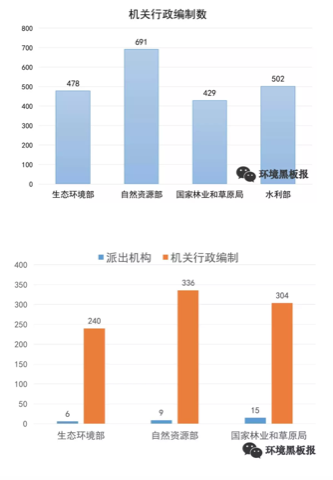
\includegraphics[width=4.62in]{images/zc1}

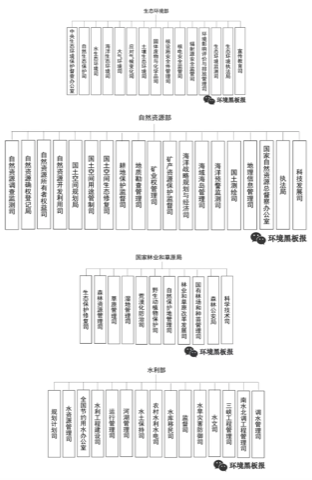
\includegraphics[width=4.33in]{images/zc2}

\hypertarget{ux4e2dux592eux56fdux52a1ux9662ux653fux7b56ux8d44ux8baf-4}{%
\subsubsection*{中央\&国务院政策资讯}\label{ux4e2dux592eux56fdux52a1ux9662ux653fux7b56ux8d44ux8baf-4}}
\addcontentsline{toc}{subsubsection}{中央\&国务院政策资讯}

\begin{itemize}
\tightlist
\item
  8月
\end{itemize}

土壤污染防治法草案进入三审 全国人大常委会同日启动海洋环境保护法执法检查。

链接 \url{http://www.mep.gov.cn/xxgk/hjyw/201808/t20180828_454296.shtml}

\hypertarget{ux751fux6001ux73afux5883ux90e8ux653fux7b56ux8d44ux8baf-4}{%
\subsubsection*{生态环境部政策资讯}\label{ux751fux6001ux73afux5883ux90e8ux653fux7b56ux8d44ux8baf-4}}
\addcontentsline{toc}{subsubsection}{生态环境部政策资讯}

\begin{itemize}
\tightlist
\item
  8月8日
\end{itemize}

生态环境部通报全国集中式饮用水水源地环境保护专项行动进展。目前,各地认真贯彻落实党中央、国务院决策部署,扎实推进饮用水水源地环境问题清理整治工作,取得阶段性成效。按照《方案》要求,各地排查县级及以上饮用水水源地2466个,发现环境问题6426个。水源保护区内存在的环境问题,主要包括:生活面源污染、工业企业排污、农业面源污染、旅游餐饮污染、交通穿越等项目,分别占问题总数的27\%、16\%、16\%、14\%、13\%。各地按照``一个水源地、一套方案、一抓到底''的要求,均已建立问题清单管理制度,对排查出来的问题建档立案,为下一步清理整治奠定了较好的基础。

链接 \url{http://www.mep.gov.cn/gkml/sthjbgw/qt/201808/t20180808_451049.htm}

\begin{itemize}
\tightlist
\item
  8月15日
\end{itemize}

按照《大气污染防治法》相关规定和国务院印发的《打赢蓝天保卫战三年行动计划》要求,近日生态环境部会同市场监管总局发布了《环境空气质量标准》(GB 3095-2012)修改单,修改了标准中关于监测状态的规定,并修改完善了相应的配套监测方法标准,实现了与国际接轨。。

链接 \url{http://www.mep.gov.cn/gkml/sthjbgw/qt/201808/t20180815_451395.htm}

\begin{itemize}
\tightlist
\item
  8月21日
\end{itemize}

``绿盾2018''自然保护区监督检查专项行动巡查拉开帷幕。由生态环境部、自然资源部、水利部、农业农村部和中国科学院等5部门联合组成组成12个组;进行为期1个月的专项巡查。首批3个巡查组分赴天津、甘肃和广东。

链接 \url{http://www.mep.gov.cn/xxgk/hjyw/201808/t20180823_452432.shtml}

相关回馈

湖北自然保护区问题整改取得积极进展

\url{https://www.huanbao-world.com/a/quanguo/hubei/37896.html}

甘肃祁连山国家级自然保护区神树水电站生态破坏问题整改不到位

\url{http://www.cenews.com.cn/news/201808/t20180829_883783.html}

甘肃小陇山国家级自然保护区未执行生态流量保障要求

\url{https://baijiahao.baidu.com/s?id=1609951111027544705\&wfr=spider\&for=pc}

福建漳江口红树林国家级自然保护区核心区存在大量养殖设施

\url{https://baijiahao.baidu.com/s?id=1609951180324037719\&wfr=spider\&for=pc}

\begin{itemize}
\tightlist
\item
  8月27日
\end{itemize}

中央电视台报道国务院第十八督查组在湖南株洲核查污水直排时,发现株洲市醴陵王坊水质自动监测站的水质监测探头插入矿泉水瓶,涉嫌数据造假。对此,生态环境部连夜调度,立即组建由环境管理、环境执法、地方环保人员以及监测专家组成的调查组,于8月28日赶赴现场进行调查。

链接 \url{http://www.mep.gov.cn/gkml/sthjbgw/qt/201808/t20180828_454324.htm}

\begin{itemize}
\tightlist
\item
  8月28日
\end{itemize}

生态环境部常务会议,审议并原则通过《关于生态环境领域进一步深化``放管服''改革 推动经济高质量发展的指导意见》和《柴油车污染物排放限值及测量方法(自由加速法和加载减速法)》《汽油车污染物排放限值及测量方法(双怠速法及简易工况法)》两项污染物排放标准。

链接 \url{http://www.mep.gov.cn/gkml/sthjbgw/qt/201808/t20180829_454356.htm}

\begin{itemize}
\tightlist
\item
  联合发布
\end{itemize}

自然资源部、中国工商银行近日联合印发《关于促进海洋经济高质量发展的实施意见》(以下简称《实施意见》)。《实施意见》明确了双方下一步推动海洋经济高质量发展的工作目标、重点领域、重点区域、服务方式、合作机制等内容,以深入贯彻党的十九大关于``加快建设海洋强国''``增强金融服务实体经济能力''``加强生态保护修复''和中央经济工作会关于``推动高质量发展''的战略部署。《实施意见》落实了《全国海洋经济发展``十三五''规划》和《关于改进和加强海洋经济发展金融服务的指导意见》要求,将推动海洋经济的高质量发展。

链接 \url{http://www.mlr.gov.cn/xwdt/jrxw/201808/t20180828_2183527.htm}

\hypertarget{ux4e5dux6708}{%
\section*{九月}\label{ux4e5dux6708}}
\addcontentsline{toc}{section}{九月}

\hypertarget{ux7814ux7a76ux52a8ux6001-10}{%
\subsection*{研究动态}\label{ux7814ux7a76ux52a8ux6001-10}}
\addcontentsline{toc}{subsection}{研究动态}

\begin{itemize}
\tightlist
\item
  用类似于代谢组学的方法测定生牛奶,巴士杀菌奶,和UHT灭菌奶中的化学成分特征。此研究发现氧化脂类可以作为区分不同奶产品的标志物(marker)。
\end{itemize}

推荐人:田振宇

链接:\url{https://www.journalofdairyscience.org/article/S0022-0302(18)30787-2/fulltext}

\begin{itemize}
\tightlist
\item
  如果把城市看作一个整体,那么农产品在城市与农田间的传输也可以看成一种进出口,有人据此绘制了美国都会区的农产品进出口分布图,近八成都会区是需要进口农产品的,这种城乡输血关系在国内也客观存在,经济上的等价交换不一定反映了资源空间上的合理配置,这为可持续城市规划设计提供了基础数据
\end{itemize}

推荐人:于淼

链接:\url{https://pubs.acs.org/doi/10.1021/acs.est.7b06462}

\begin{itemize}
\tightlist
\item
  一般认为DNA比RNA稳定,这篇研究测试了单链/双链+DNA/RNA的光解速率常数,发现双链比单链稳定,RNA比DNA稳定,这个结果我觉得对进化研究比较有启发,可能用来解释RNA病毒的环境过程
\end{itemize}

推荐人:于淼

链接:\url{https://pubs.acs.org/doi/10.1021/acs.est.8b02308}

\begin{itemize}
\tightlist
\item
  看题目非常有意思,PFAS和猫的甲亢相关,窝就点进去看数据了。但是看了数据发现甲亢组和非甲亢组其实区别不是很大,诶。。。(王老师你不要怪我)。以及选取的猫都是十岁以上,大概过了这个年龄就可以算老猫了?
\end{itemize}

推荐人:田振宇

链接:\url{https://setac.onlinelibrary.wiley.com/doi/abs/10.1002/etc.4239}

\begin{itemize}
\tightlist
\item
  城市化水平原来都是各自国家报,尺度都比较大,这篇研究通过城市夜晚灯光对公里尺度上的人工物质流例如钢铁、水泥、铝制品进行回归,发现可以用来对地表物质流进行研究。这个现象其实可以深挖下,例如光谱分析
\end{itemize}

推荐人:于淼

链接:\url{https://pubs.acs.org/doi/10.1021/acs.est.8b02838}

\begin{itemize}
\tightlist
\item
  年轮不仅仅可以用来记录树的年龄,也可以用来反推当时重金属污染的情况,这篇研究就用年轮很好的追溯了使用汞齐的欧洲掘金时代。年轮、冰柱、泥芯都属于环境化学中常见的反映时间尺度上物质变化的样品且相对独立,只不过采样难度不是一般的高。
\end{itemize}

推荐人:于淼

链接:\url{https://pubs.acs.org/doi/10.1021/acs.est.8b02117}

\begin{itemize}
\tightlist
\item
  现代人越来越宅,因此其实室内污染比室外污染可能更应引起关注,一个常见的说法就是开窗通气晒一下或者刷光敏油漆来除臭,不过这篇研究发现有些用来室内除臭的光敏油漆也会释放高浓度的挥发性有机污染物。
\end{itemize}

推荐人:于淼

链接:\url{https://pubs.acs.org/doi/10.1021/acs.est.8b03865}

\begin{itemize}
\tightlist
\item
  这是一篇标准的跨学科灌水文,很多地方概念都是错的,而且要是让真正做机器学习的看到估计还以为是个课后习题。
\end{itemize}

推荐人:于淼

链接:\url{https://pubs.acs.org/doi/10.1021/acs.est.8b03328}

\begin{itemize}
\tightlist
\item
  现在做非目的分析的同学越来越多,这篇来自EPA的文章对使用工具进行了很好的综述,推荐阅读
\end{itemize}

推荐人:于淼

链接:\url{https://www.nature.com/articles/s41370-017-0012-y}

\hypertarget{ux653fux7b56ux901fux9012-5}{%
\subsection*{政策速递}\label{ux653fux7b56ux901fux9012-5}}
\addcontentsline{toc}{subsection}{政策速递}

\hypertarget{ux91cdux5927ux653fux7b56ux8d44ux8baf-5}{%
\subsubsection*{重大政策资讯}\label{ux91cdux5927ux653fux7b56ux8d44ux8baf-5}}
\addcontentsline{toc}{subsubsection}{重大政策资讯}

\begin{itemize}
\tightlist
\item
  2018年9月
\end{itemize}

中共中央、国务院印发《乡村振兴战略规划(2018---2022年)》,对实施乡村振兴战略第一个五年工作做出具体部署,是指导各地区各部门分类有序推进乡村振兴的重要依据。

链接 《乡村振兴战略规划(2018-2022年)》

\url{http://www.xinhuanet.com/politics/2018-09/26/c_1123487123.htm}

\hypertarget{ux4e2dux592eux56fdux52a1ux9662ux653fux7b56ux8d44ux8baf-5}{%
\subsubsection*{中央\&国务院政策资讯}\label{ux4e2dux592eux56fdux52a1ux9662ux653fux7b56ux8d44ux8baf-5}}
\addcontentsline{toc}{subsubsection}{中央\&国务院政策资讯}

\begin{itemize}
\tightlist
\item
  9月18日
\end{itemize}

国务院办公厅下发关于开展生态环境保护法规、规章、规范性文件清理工作的通知【国办发〔2018〕87号】。此次清理的范围是生态环境保护相关行政法规,省、自治区、直辖市、设区的市、自治州人民政府和国务院部门制定的规章,以及县级以上地方人民政府及其所属部门、国务院部门制定的规范性文件。清理的重点是,与习近平生态文明思想和党的十八大以来党中央、国务院有关生态环境保护文件精神,以及生态环境保护方面的法律不符合不衔接不适应的规定。

链接 \url{http://www.gov.cn/zhengce/content/2018-09/18/content_5322978.htm}

\begin{itemize}
\tightlist
\item
  9月27日
\end{itemize}

中共中央办公厅、国务院办公厅印发《海南省机构改革方案》。这是全国首个获得党中央、国务院批准的地方机构改革方案。改革后,海南省将设置党政机构55个,其中省委机构18个、政府机构37个,同中央和国家机关保持总体一致,也体现了海南特色。同日,海南省机构改革动员大会在省人大会堂召开,省委书记、省人大常委会主任作动员讲话。

链接 \url{http://www.hainan.gov.cn/data/news/2018/09/181852/}

\hypertarget{ux751fux6001ux73afux5883ux90e8ux653fux7b56ux8d44ux8baf-5}{%
\subsubsection*{生态环境部政策资讯}\label{ux751fux6001ux73afux5883ux90e8ux653fux7b56ux8d44ux8baf-5}}
\addcontentsline{toc}{subsubsection}{生态环境部政策资讯}

\begin{itemize}
\tightlist
\item
  9月2日
\end{itemize}

在国家主席与南非总统见证下,生态环境部部长和南非环境部部长分别代表各自政府,在人民大会堂共同签署了《中华人民共和国政府与南非共和国政府关于气候变化领域合作的谅解备忘录》(简称《备忘录》)。根据《备忘录》,双方将在碳排放交易,绿色低碳城镇化,碳捕集、利用和封存技术,温室气体信息汇编与温室气体数据库管理等优先领域开展合作,并将共同加强气候变化领域能力建设。

链接 \url{http://www.mee.gov.cn/gkml/sthjbgw/qt/201809/t20180905_549331.htm}

\begin{itemize}
\tightlist
\item
  9月21日
\end{itemize}

生态环境部批准《环境影响评价技术导则 土壤环境(试行)》为国家环境保护标准,并予发布,以贯彻《中华人民共和国环境保护法》和《中华人民共和国环境影响评价法》,保护土壤环境质量,管控土壤污染风险。该标准自2019年7月1日起实施。

链接 \url{http://www.mee.gov.cn/gkml/sthjbgw/sthjbgg/201809/t20180921_626417.htm}

\begin{itemize}
\tightlist
\item
  9月21日
\end{itemize}

生态环境部发布``关于进一步强化生态环境保护监管执法的意见'',以贯彻落实党中央、国务院决策部署,坚决纠正违法排污乱象,压实企业及其主要负责人生态环境保护责任,推动守法成为常态。意见包括:落实企业主要负责人第一责任、全面推行``双随机、一公开''、 利用科技手段精准发现违法问题、实施群众关切问题预警督办制度、集中力量查处大案要案、制定发布权力清单和责任清单、严格禁止``一刀切''。

链接 \url{http://www.mee.gov.cn/gkml/sthjbgw/bgtwj/201809/t20180927_630564.htm}

\begin{itemize}
\tightlist
\item
  9月26日
\end{itemize}

生态环境部就侵占破坏自然保护区问题约谈辽宁锦州、吉林延边、江苏镇江、安徽宣城、重庆沙坪坝区和北碚区、云南丽江和西双版纳等8市(州、区)政府和有关部门,要求严格自然保护区管理,推进中央环保督察和``绿盾2017''整改落实,禁止以损害自然保护区为代价谋求一时一地经济增长。

链接 \url{http://www.mee.gov.cn/gkml/sthjbgw/qt/201809/t20180926_629613.htm}

\begin{itemize}
\tightlist
\item
  9月27日
\end{itemize}

7省(市)公开中央环境保护督察整改落实情况。

经党中央、国务院批准,中央环境保护督察组于2017年4月至5月组织对天津、山西、辽宁、安徽、福建、湖南、贵州等7省(市)开展环境保护督察,并于2017年8月完成督察反馈。督察反馈后,7省(市)党委、政府高度重视,将环境保护督察整改作为政治责任来担当,作为推进生态文明建设和环境保护的重要抓手,建立机制,强化措施,狠抓落实,取得明显的整改成效。截至2018年9月中旬,7省(市)督察整改方案明确的531项整改任务已完成313项,其余正在推进中。通过督察整改,一批长期难以解决的环境问题得到了解决,一批长期想办的事情得到了落实

链接

天津市对外公开中央环境保护督察整改情况

\url{http://www.mee.gov.cn/gkml/sthjbgw/qt/201809/t20180928_632821.htm}

山西省对外公开中央环境保护督察整改情况

\url{http://www.mee.gov.cn/gkml/sthjbgw/qt/201809/t20180928_632822.htm}

辽宁省对外公开中央环境保护督察整改情况

\url{http://www.mee.gov.cn/gkml/sthjbgw/qt/201809/t20180928_632823.htm}

安徽省对外公开中央环境保护督察整改情况

\url{http://www.mee.gov.cn/gkml/sthjbgw/qt/201809/t20180928_632824.htm}

福建省对外公开中央环境保护督察整改情况

\url{http://www.mee.gov.cn/gkml/sthjbgw/qt/201809/t20180928_632825.htm}

湖南省对外公开中央环境保护督察整改情况

\url{http://www.mee.gov.cn/gkml/sthjbgw/qt/201809/t20180928_632826.htm}

贵州省对外公开中央环境保护督察整改情况

\url{http://www.mee.gov.cn/gkml/sthjbgw/qt/201809/t20180928_632827.htm}

\hypertarget{ux5341ux6708}{%
\section*{十月}\label{ux5341ux6708}}
\addcontentsline{toc}{section}{十月}

\hypertarget{ux7814ux7a76ux52a8ux6001-11}{%
\subsection*{研究动态}\label{ux7814ux7a76ux52a8ux6001-11}}
\addcontentsline{toc}{subsection}{研究动态}

\begin{itemize}
\tightlist
\item
  2017 年销售美国的奶粉和牛奶中依然能检出微量的三聚氰胺,虽然浓度比 2008 年的毒奶粉要低很多。另外液体配方奶比奶粉中三聚氰胺浓度更高。持续的低浓度污染可能是来自养奶牛的饲料。
\end{itemize}

推荐人:田振宇

链接:\url{https://pubs.acs.org/doi/10.1021/acs.estlett.8b00515}

\begin{itemize}
\tightlist
\item
  虽然媒体报道富营养化是少了,但现状其实一直在恶化,这篇研究关注了墨西哥湾海洋低溶解氧区的时空分布特征,我国近海也存在这个问题且对渔业影响很大。
\end{itemize}

推荐人:于淼

链接:\url{https://pubs.acs.org/doi/10.1021/acs.est.8b03474}

\begin{itemize}
\tightlist
\item
  很多人可能没意识到美国经过页岩气革命已经是能源出口国了,天然气替代煤炭石油作为燃料本身是可以降低二氧化碳排放的,但是这篇研究发现天然气开采点附近的甲烷泄露却是区域内的峰值,而甲烷也是温室气体。
\end{itemize}

推荐人:于淼

链接:\url{https://pubs.acs.org/doi/10.1021/acs.est.8b03535}

\begin{itemize}
\tightlist
\item
  美国儿童肥胖问题已经是根深蒂固了,这篇研究探索了三百来个可能造成儿童肥胖的有关因素,用随机森林法发现大部分高危险因素都是社会性因素(比如这个学区的犯罪率之类的),而不是通常认为的环境因素(比如周围有多少免费的运动场)。机器学习的方法夺人眼球,加州的杰瑞特教授从来都不拒绝把眩酷科技带入传统的流行病学方法里。
\end{itemize}

推荐人:张雪莹

链接:\url{https://www.sciencedirect.com/science/article/pii/S0013935118302226}

\begin{itemize}
\tightlist
\item
  Hites 老爷子对 non-target screening 的一些问题和建议,主要集中在可重复性问题。有很多非常中肯的观点,虽然也有一些值得商榷。
\end{itemize}

推荐人:田振宇

链接:\url{https://pubs.acs.org/doi/10.1021/acs.est.8b05671}

\begin{itemize}
\tightlist
\item
  近年来越来越多的流行病学研究登上曾经被自然科学占领的 Nature 期刊。俗话说''3 岁看小,7 岁看老 ``,通过检查小时候的肠道菌群能看出长大后患一型糖尿病的概率。母乳喂养依然是建立肠道菌落多样性的最重要因素。此外,家里有兄弟姐妹和毛绒宠物也很重要。这一期 Nature 还同时接收了同一项目的另一篇有关儿童建立肠道菌群的文章。推荐理由是幼儿的肠道菌群还在建立的过程中,相关地代谢组酶组也不是太稳定,这两篇文章提供了不少日后研究幼儿组学的参考。
\end{itemize}

推荐人:张雪莹

链接: \url{https://www.nature.com/articles/s41586-018-0620-2}

\begin{itemize}
\tightlist
\item
  又一篇 view point, 关于机器学习(machine learning)在环境毒理方面的应用,作者认为 ML 在这个领域应该有更好的应用,但目前接受度以及实际工作的水平还不够。尤其是作者提出的 ``ML-literate scientists'' 这个概念很有意思。
\end{itemize}

推荐人:田振宇

链接:\url{https://pubs.acs.org/doi/10.1021/acs.est.8b05382}

\begin{itemize}
\tightlist
\item
  远洋货轮为了控制首要污染物会采用低硫燃料,然而这篇研究发现低硫燃料却导致了更多中等挥发性有机污染物的释放,污染控制中针对性的控制手段往往按下葫芦瓢起来,需要综合考量,不过这又绕到了 unknown unknown 的困境中了,还是先摸着石头过河吧。
\end{itemize}

推荐人:于淼

链接:\url{https://pubs.acs.org/doi/10.1021/acs.est.8b04418}

\begin{itemize}
\tightlist
\item
  也是 viewpoint,很多污染物的环境行为是跟政治经济技术有直接关系的,中国修改了钢铁标准中钒的量,然后 2017 年钒矿石价格直接翻倍,增多的钒矿会导致更多的钒释放到环境中,然后有人发现钒的污染自上世纪七十年代减少后又重新升高了。正是因为这些错综复杂的关系,才让环境研究既有意思也很难进行控制实验。
\end{itemize}

推荐人:于淼

链接:\url{https://pubs.acs.org/doi/10.1021/acs.est.8b05560}

\hypertarget{ux7814ux7a76ux7b80ux62a5-2}{%
\subsection*{805研究简报}\label{ux7814ux7a76ux7b80ux62a5-2}}
\addcontentsline{toc}{subsection}{805研究简报}

本栏目旨在介绍805班同学发表的论文

\hypertarget{ux975eux76eeux7684ux68c0ux6d4bux4e2dux7684ux7ed3ux6784-ux53cdux5e94ux5f15ux5bfcux5206ux6790---ux4e8eux6dfc}{%
\subsubsection*{非目的检测中的结构 / 反应引导分析 - 于淼}\label{ux975eux76eeux7684ux68c0ux6d4bux4e2dux7684ux7ed3ux6784-ux53cdux5e94ux5f15ux5bfcux5206ux6790---ux4e8eux6dfc}}
\addcontentsline{toc}{subsubsection}{非目的检测中的结构 / 反应引导分析 - 于淼}

质谱非目的分析的一个难点在于冗余峰比较多,单一化合物在高分辨全扫描模式下会存在同位素、加合物、粒子碎片、中性丢失等多种峰,这些峰的响应往往高度相关,后续的统计分析如果不考虑这种内在的均质性,分析结果是有偏的,能在离子化过程出现更多峰的化合物会有更高的权重。针对这一问题,我开发了 GlobalStd 算法,通过同一保留时间聚类中高频出现的质量差来推测属于同一物质的离子峰并选择出可能的分子离子峰,这里我没有使用相关性来判断是因为物质间可能存在天然的相关性。实验结果显示 20\% 的峰即可保留原有数据中的异质性。

在不进行注释的情况下,我提出了结构 / 反应引导分析,原理就是基于 GlobalStd 算法得出的代表性峰间的质量差异来推测其可能涉及的生化反应,例如羟基化过程可能伴随 16 的质量差。如果该质量差高频出现,那么这就说明这类反应可能比较重要,实验数据也很好地支持了这个假设。这样,我们可以直接用所有涉及该反应的峰来定量特定的反应过程,从而跳过具体的注释过程来探索生物样品中的已知 / 未知生化反应。

GlobalStd 算法与结构 / 反应引导分析被我打包成 pmd 软件包且通过 shiny 提供了图形化界面,可以很好地耦合进基于 xcms 的数据分析流程。实验原始数据也封装进了 pmd 软件包。

链接:\url{https://www.sciencedirect.com/science/article/pii/S0003267018313047}

pmd 包网站:\url{https://yufree.github.io/pmd/}

\hypertarget{ux653fux7b56ux901fux9012-6}{%
\subsection*{政策速递}\label{ux653fux7b56ux901fux9012-6}}
\addcontentsline{toc}{subsection}{政策速递}

\hypertarget{ux91cdux5927ux653fux7b56ux8d44ux8baf-6}{%
\subsubsection*{重大政策资讯}\label{ux91cdux5927ux653fux7b56ux8d44ux8baf-6}}
\addcontentsline{toc}{subsubsection}{重大政策资讯}

\begin{itemize}
\tightlist
\item
  2018年10月9日
\end{itemize}

中共中央办公厅印发《关于统筹规范督查检查考核工作的通知》,以更好推动党的十九大精神和党中央决策部署贯彻落实,深入推进全面从严治党,进一步改进工作作风,坚决克服形式主义、官僚主义。就是说,以后各级督查检查(包括环保督查)也要按章办事、考虑实际、控制总量了。

链接: \url{http://www.gov.cn/xinwen/2018-10/09/content_5328884.htm}

\hypertarget{ux4e2dux592eux56fdux52a1ux9662ux653fux7b56ux8d44ux8baf-6}{%
\subsubsection*{中央\&国务院政策资讯}\label{ux4e2dux592eux56fdux52a1ux9662ux653fux7b56ux8d44ux8baf-6}}
\addcontentsline{toc}{subsubsection}{中央\&国务院政策资讯}

\begin{itemize}
\tightlist
\item
  9月24日
\end{itemize}

国务院办公厅印发关于完善促进消费体制机制实施方案(2018---2020年)的通知,生态环境部所分到的工作包括促进汽车消费优化升级、发展壮大绿色消费、加强消费产品和服务标准制定、加强消费领域统计监测、认真做好消费宣传引导等,主旨在于推进绿色消费、绿色产品标准体系。

链接: \url{http://www.gov.cn/zhengce/content/2018-10/11/content_5329516.htm}

\begin{itemize}
\tightlist
\item
  10月9日
\end{itemize}

国务院办公厅印发关于推进运输结构调整三年行动计划(2018---2020年)的通知,提及城市绿色配送行动,积极落实财政等支持政策中,指出要贯彻落实《国务院关于印发打赢蓝天保卫战三年行动计划的通知》(国发〔2018〕22号)有关要求,对大力淘汰老旧车辆、推广应用新能源汽车的有关企业和人员依照有关政策及时给予经济补偿。

链接 \url{http://www.gov.cn/zhengce/content/2018-10/09/content_5328817.htm}

\begin{itemize}
\tightlist
\item
  10月15日
\end{itemize}

国务院办公厅印发《关于加强长江水生生物保护工作的意见》。长江是中华民族的母亲河,是中华民族发展的重要支撑。多年来,受拦河筑坝、水域污染、过度捕捞、航道整治、岸坡硬化、挖砂采石等人类活动影响,长江生物多样性持续下降,水生生物保护形势严峻,水域生态修复任务艰巨。国务院为加强长江水生生物保护工作,提出此意见文件。主要包括总体要求、开展生态修复、拯救濒危物种、加强生境保护、完善生态补偿、加强执法监管、强化支撑保障、加强组织领导等方面。

链接: \url{http://www.gov.cn/zhengce/content/2018-10/15/content_5330882.htm}

\begin{itemize}
\tightlist
\item
  10月24日
\end{itemize}

为更好实现国有资产综合报告``全口径''、``全覆盖''的目标,实现各类国有资产管理、报告、监督的全流程闭环,10月24日上午,国务院就2017年度国有资产管理情况向十三届全国人大常委会第六次会议作《国务院关于2017年度国有资产管理情况的综合报告》。这在国内尚属首次。其中叙述我国2017年国有自然资源资产情况包括:国有土地面积5.05亿公顷,内水和领海面积38万平方公里,天然气剩余技术可采储量5.5万亿立方米,等。同时,国有自然资源资产管理情况和下一步工作安排也有阐述。

链接: \url{http://www.npc.gov.cn/npc/xinwen/2018-10/25/content_2063928.htm}

\begin{itemize}
\tightlist
\item
  10月26日
\end{itemize}

第十三届全国人民代表大会常务委员会第六次会议通过15部法律修改的决定,主要修改内容多是国家机构改革之后各主管部门的调整。其中与生态环境相关的有7部:《中华人民共和国野生动物保护法》、《中华人民共和国大气污染防治法》、《中华人民共和国节约能源法》、《中华人民共和国防沙治沙法》、《中华人民共和国农产品质量安全法》、《中华人民共和国循环经济促进法》、《中华人民共和国环境保护税法》。

链接: \url{http://www.gov.cn/xinwen/2018-10/27/content_5334907.htm}

\begin{itemize}
\tightlist
\item
  10月29日
\end{itemize}

国务院印发《关于严格管制犀牛和虎及其制品经营利用活动的通知》,犀牛和虎是国内外广泛关注的珍稀濒危野生动物。根据《中华人民共和国野生动物保护法》等法律法规和《濒危野生动植物种国际贸易公约》等国际公约的规定,为加强对犀牛和虎的保护,有力打击犀牛和虎及其制品非法贸易,严格管制犀牛和虎及其制品经营和利用等活动,印发《通知》。

链接: \url{http://www.gov.cn/zhengce/content/2018-10/29/content_5335423.htm}

\hypertarget{ux751fux6001ux73afux5883ux90e8ux653fux7b56ux8d44ux8baf-6}{%
\subsubsection*{生态环境部政策资讯}\label{ux751fux6001ux73afux5883ux90e8ux653fux7b56ux8d44ux8baf-6}}
\addcontentsline{toc}{subsubsection}{生态环境部政策资讯}

\begin{itemize}
\tightlist
\item
  10月15日
\end{itemize}

《打好污染防治攻坚战宣传工作方案(2018---2020年)》为进一步推动生态环境宣传工作上台阶上水平,营造打好污染防治攻坚战良好舆论氛围,形成人人关心、支持、参与生态环境保护工作的局面,生态环境部日前印发此方案。

链接: \url{http://www.mee.gov.cn/xxgk2018/xxgk/xxgk15/201810/t20181015_662363.html}

\begin{itemize}
\tightlist
\item
  10月24日
\end{itemize}

为履行《保护臭氧层维也纳公约》和《关于消耗臭氧层物质的蒙特利尔议定书》(以下简称议定书),生态环境部近日印发《关于禁止生产以一氟二氯乙烷(HCFC-141b)为发泡剂的冰箱冷柜产品、冷藏集装箱产品、电热水器产品的公告》

链接: \url{http://www.mee.gov.cn/xxgk2018/xxgk/xxgk15/201810/t20181024_665324.html}

有关该公告的专家解读:

链接: \url{http://www.mee.gov.cn/xxgk2018/xxgk/xxgk15/201810/t20181024_665325.html}

\begin{itemize}
\tightlist
\item
  10月25日
\end{itemize}

为贯彻党中央、国务院关于打赢蓝天保卫战决策部署,落实《打赢蓝天保卫战三年行动计划》,全力做好2018-2019年秋冬季大气污染防治工作,汾渭平原大气污染防治协作小组第一次全体会议审议通过了《汾渭平原2018-2019年秋冬季大气污染综合治理攻坚行动方案》。

链接: \url{http://www.mee.gov.cn/xxgk2018/xxgk/xxgk03/201810/t20181029_667650.html}

\begin{itemize}
\tightlist
\item
  10月30日
\end{itemize}

生态环境部通报表扬安徽、福建、广西3地环境违法犯罪案件办理工作,三省分别针对严重的工业固废、危险废物跨省非法转移、倾倒污染环境案件进行处理。三省环保部门在案件查办过程中,充分发扬特别能吃苦、特别能战斗、特别能奉献的生态环境保护铁军精神,省、市、县三级环保部门通力合作,监察执法、环境监测、固体废物管理、应急管理等部门密切配合,部署周密、措施果断、行动迅速,通过运用``两法衔接''机制,强化刑事打击手段,切实发挥刑责治污的惩戒和警示作用。

链接: \url{http://www.mee.gov.cn/xxgk2018/xxgk/xxgk15/201810/t20181030_670129.html}

\begin{itemize}
\tightlist
\item
  10月15日
\end{itemize}

住房城乡建设部、生态环境部联合发布《城市黑臭水体治理攻坚战实施方案》,重在进一步落实2015年国务院印发的《水污染防治行动计划》,扎实推进城市黑臭水体治理工作。涉及部门包括:住建部、发改委、财政部、生态环境部、自然资源部、水利部、工信部、农业农村部、组织部、人民银行、银保监会、证监会、科技部等,各城市人民政府负责落实。好奇各部门做什么?看文件吧\textasciitilde{}

链接: \url{http://www.mohurd.gov.cn/wjfb/201810/t20181015_237912.html}

\hypertarget{ux5341ux4e00ux6708-1}{%
\section*{十一月}\label{ux5341ux4e00ux6708-1}}
\addcontentsline{toc}{section}{十一月}

\hypertarget{ux7814ux7a76ux52a8ux6001-12}{%
\subsection*{研究动态}\label{ux7814ux7a76ux52a8ux6001-12}}
\addcontentsline{toc}{subsection}{研究动态}

\begin{itemize}
\tightlist
\item
  当前环境研究细分领域越来越多,我们越来越倾向于回答那些特定污染物在特定区域的问题,然而,对大尺度区域里污染物的整体考量也很重要,这份研究探索了细颗粒物在全球尺度上的日浓度分布,给了一个整体估计,这种全球尺度的基线数据值得关注。
\end{itemize}

推荐人:于淼

链接:\url{https://pubs.acs.org/doi/10.1021/acs.estlett.8b00573}

\begin{itemize}
\tightlist
\item
  国内关于室内污染的研究多借鉴国外的方法与思路,不过我想提醒的是生活习惯差异是需要考虑的,例如国内室内一般不用地毯,用地毯也会另配拖鞋,但国外地毯经常是光着脚踩,这种习惯差异本身就会导致暴露量估计的差异。同样,国内建筑的通风设计与采暖标准跟海外也有较大差异,模型应该对此进行相应的调整。
\end{itemize}

推荐人:于淼

链接:\url{https://pubs.acs.org/doi/10.1021/acs.est.8b03580}

\begin{itemize}
\tightlist
\item
  也是关于室内污染的,二手烟指的是别人抽你吸,三手烟则指别人抽完了,房间吸收了,然后缓慢释放出来,这篇研究发现不同的污染物会分布到不同的气溶胶中,可以考虑与生物有效性结合下理解。
\end{itemize}

推荐人:于淼

链接:\url{https://pubs.acs.org/doi/10.1021/acs.est.8b03580}

\begin{itemize}
\tightlist
\item
  粮食需求要求农业的集约化生产,这篇文章详细讨论了全球尺度农业集约化可能带来的环境影响,主要是对氮排放的讨论,这是一篇基线数据报告,不过如果能结合全球气候变化进行讨论就更好了。
\end{itemize}

推荐人:于淼

链接:\url{https://pubs.acs.org/doi/10.1021/acs.est.8b03610}

\begin{itemize}
\tightlist
\item
  轮胎磨损会产生橡胶颗粒,这篇文章用底栖动物考察了生态毒理影响,结果发现影响有限,作者进一步讨论了不同淋洗所可能造成的毒性,认为过高的毒性报道可能来自于过激的采样萃取过程,颗粒中污染物的生物有效性可能并不高。环境分析化学的一个特性就是真实环境条件下的浓度分析,生物有效性问题值得结合调查数据进行深入讨论。
\end{itemize}

推荐人:于淼

链接:\url{https://pubs.acs.org/doi/10.1021/acs.est.8b05035}

\begin{itemize}
\tightlist
\item
  短链氯化石蜡是一类同分异构体与同系物接近天文数字的污染物,而中链与长链氯化石蜡在这方面问题更大,面对这种滚刀肉,学术界需要就分析方法与标准达成一致,这篇文章就针对这个问题进行了详细讨论,相信对进行系列污染物例如双酚类、全氟类与eDNA分析方法研究的同学也会有启发性。
\end{itemize}

推荐人:于淼

链接:\url{https://pubs.acs.org/doi/10.1021/acs.estlett.8b00537}

\begin{itemize}
\tightlist
\item
  Bruce E. Logan 的日常吐槽,川普喜欢建边境隔离墙而不喜欢气候变化,但事实上全球变暖引发的海平面上升也需要构建防波堤来减少影响,这方面花的也不比边境隔离墙少多少,而且边境墙不一定有必要但防波堤对沿海地区几乎是唯一选择,哪怕他们不信气候变化也不能防止海水倒灌。减少化石燃料使用与开发新能源可能是唯一的道路。
\end{itemize}

推荐人:于淼

链接:\url{https://pubs.acs.org/doi/10.1021/acs.estlett.8b00572}

\begin{itemize}
\tightlist
\item
  同位素在环境化学里是神器般的存在,放射性同位素可以示踪,稳定同位素如果十分稳定可以溯源,如果不稳定可以指示环境过程,这篇研究就发现锶的稳定同位素可以用来指示燃烧源,在水环境与鱼中都比较稳定。
\end{itemize}

推荐人:于淼

链接:\url{https://pubs.acs.org/doi/10.1021/acs.estlett.8b00477}

\begin{itemize}
\tightlist
\item
  美国这边道路畅通的一个重要原因是遇上下雪后撒盐跟不要钱一样,均下来一人一年撒盐62.1kg,这个量已经足够产生环境影响了,这篇文章发现撒盐已经实质上影响了私人井的水质并对建筑结构产生了腐蚀,可以算是一种公地悲剧吧
\end{itemize}

推荐人:于淼

链接:\url{https://pubs.acs.org/doi/10.1021/acs.est.8b04709}

\hypertarget{ux5341ux4e00ux6708ux73afux5883ux65b0ux95fbux65b0ux653f}{%
\subsection*{十一月环境新闻新政}\label{ux5341ux4e00ux6708ux73afux5883ux65b0ux95fbux65b0ux653f}}
\addcontentsline{toc}{subsection}{十一月环境新闻新政}

\hypertarget{ux4e2dux592eux56fdux5bb6ux5c42ux9762}{%
\subsubsection*{中央国家层面}\label{ux4e2dux592eux56fdux5bb6ux5c42ux9762}}
\addcontentsline{toc}{subsubsection}{中央国家层面}

\begin{itemize}
\tightlist
\item
  \href{https://www.mfa.gov.cn/web/ziliao_674904/1179_674909/t1613067.shtml}{11月14日,中华人民共和国政府和加拿大政府关于应对海洋垃圾和塑料的联合声明}
\end{itemize}

中华人民共和国国务院总理李克强与加拿大总理贾斯廷·特鲁多于新加坡举行第三次中加总理年度对话。双方认识到,当前人类活动造成的塑料污染给海洋健康、生物多样性及可持续发展带来负面影响,对人体健康构成潜在风险。双方认为,采取可持续的全生命周期法管理塑料,对减轻塑料对环境的威胁,尤其是对减少海洋垃圾具有重要意义。

\textbf{延伸阅读}

\begin{itemize}
\item
  \href{http://tech.ifeng.com/a/20181028/45202181_0.shtml}{奥地利的一项研究称,在人体内发现了多达9种不同种类的微塑料,大小从0.05-0.5毫米不等,比头发丝还小几倍。其中最常见的为聚丙烯(PP)和聚对苯二甲酸乙二醇酯(PET),这两者都是矿泉水瓶的主要材料。}
\item
  \href{http://news.ifeng.com/a/20180906/60032654_0.shtml}{自来水中也有微塑料}
\end{itemize}

美国明尼苏达大学等研究团队发现,在全球13个国家的自来水、欧美和亚洲产食盐以及美国产的啤酒中,广泛存在引发全球性污染问题的``微塑料''。研究团队分析了在美国、英国、古巴和印度等14个国家采集的159份自来水样本。除意大利之外的13个国家的样本中都发现了微塑料。

\begin{itemize}
\tightlist
\item
  \href{https://baijiahao.baidu.com/s?id=1617711608828470969\&wfr=spider\&for=pc}{鲸鱼搁浅,胃内剖出将近6千克塑料垃圾}
\end{itemize}

2018年11月20日,印度尼西亚瓦卡托比国家公园发现一头抹香鲸的尸体。研究人员解剖后发现将近6千克的塑料垃圾,包括115个塑料杯、25个塑料袋、4个塑料瓶、2只拖鞋、一个尼龙袋和超过1000块塑料制品残余。

\hypertarget{ux56fdux52a1ux9662}{%
\subsubsection*{国务院}\label{ux56fdux52a1ux9662}}
\addcontentsline{toc}{subsubsection}{国务院}

\begin{itemize}
\tightlist
\item
  \href{http://www.gov.cn/xinwen/2018-11/29/content_5344537.htm}{11月29日,中共中央国务院《关于建立更加有效的区域协调发展新机制的意见》,《意见》提出要加快形成统筹有力、竞争有序、绿色协调、共享共赢的区域协调发展新机制,促进区域协调发展。《意见》全文多处与《生态文明体制改革总体方案》高度衔接,将生态文明建设贯穿各方面。例如``健全市场一体化发展机制'' 中提出``完善区域交易平台和制度'',包括自然资源资产有偿使用制度、统一的自然资源资产交易平台等;``健全区际利益补偿机制''中明确,完善多元化横向生态补偿机制。}
\end{itemize}

\hypertarget{ux56fdux5bb6ux53d1ux6539ux59d4}{%
\subsubsection*{国家发改委}\label{ux56fdux5bb6ux53d1ux6539ux59d4}}
\addcontentsline{toc}{subsubsection}{国家发改委}

\begin{itemize}
\tightlist
\item
  \href{http://www.ndrc.gov.cn/zcfb/zcfbghwb/201811/t20181107_919133.html}{11月2日,国家发改委印发《淮河生态经济带发展规划》,要求以供给侧结构性改革为主线,坚决打好防范化解重大风险、精准脱贫、污染防治三大攻坚战,着力推进绿色发展,改善淮河流域生态环境,实施创新驱动发展战略,深化体制机制改革,构建全方位开放格局,促进区域协调发展,推动经济发展质量变革、效率变革、动力变革,建设现代化经济体系,增进民生福祉,加快建成美丽宜居、充满活力、和谐有序的生态经济带。}
\end{itemize}

\hypertarget{ux751fux6001ux73afux5883ux90e8}{%
\subsubsection*{生态环境部}\label{ux751fux6001ux73afux5883ux90e8}}
\addcontentsline{toc}{subsubsection}{生态环境部}

\begin{itemize}
\tightlist
\item
  \href{http://www.ywrp.gov.cn/bzgf/6253.html}{11月6日,生态环境部印发《长江流域水环境质量监测预警办法(试行)》,要求以``和谐长江、健康长江、清洁长江、优美长江和安全长江''为目标,以水环境质量只能变好、不能变差为原则,加快建立长江流域自动监测管理和技术体系,完善长江流域国家地表水环境监测网络,推进长江流域水环境质量持续改善。}
\end{itemize}

\hypertarget{ux6559ux80b2ux90e8}{%
\subsubsection*{教育部}\label{ux6559ux80b2ux90e8}}
\addcontentsline{toc}{subsubsection}{教育部}

\begin{itemize}
\tightlist
\item
  \href{http://www.moe.gov.cn/srcsite/A17/moe_938/s3273/201811/t20181101_353337.htm}{11月1日,教育部归口管理的国家强制标准《中小学合成材料面层运动场地》正式实施。}
\end{itemize}

\textbf{延伸阅读}

短评:这一标准看似和生态环境没有太大关系,实则是``毒跑道''环境公益诉讼案所推动的成果。

\begin{itemize}
\item
  2016年3月底,北京刘诗昆万象新天幼儿园(``刘诗昆幼儿园'')铺设塑胶跑道并投入使用,很快家长发现,塑胶跑道散发出刺激性气味,多名幼儿出现眼睛疼、流泪、咳嗽、流鼻血等身体不适症状,家长认为这是新铺设的塑胶跑道``有毒''所导致,于是开始向有关部门反映问题。
\item
  \href{http://news.sina.com.cn/o/2018-02-05/doc-ifyreuzn3040514.shtml}{2017年4月10日,原告中国生物多样性保护与绿色发展基金会与被告刘诗昆幼儿园公益诉讼环境污染责任纠纷一案,以调解方式结案,刘诗昆幼儿园拆除园内铺设的``有毒''塑胶跑道,铺上草坪;并以保护生态环境为目的向社会捐助10万元。}
\end{itemize}

\hypertarget{ux90e8ux95e8ux8054ux5408ux53d1ux5e03}{%
\subsubsection*{部门联合发布}\label{ux90e8ux95e8ux8054ux5408ux53d1ux5e03}}
\addcontentsline{toc}{subsubsection}{部门联合发布}

\begin{itemize}
\tightlist
\item
  \href{http://www.mee.gov.cn/xxgk2018/xxgk/xxgk03/201811/t20181108672959.htm}{11月6日,生态环境部 农业农村部联合发布《农业农村污染治理攻坚战行动计划》,行动目标是通过三年攻坚,\ldots{}\ldots{}到2020年,实现``一保两治三减四提升'':``一保'',即保护农村饮用水水源,农村饮水安全更有保障;``两治'',即治理农村生活垃圾和污水,实现村庄环境干净整洁有序;``三减'',即减少化肥、农药使用量和农业用水总量;``四提升'',即提升主要由农业面源污染造成的超标水体水质、农业废弃物综合利用率、环境监管能力和农村居民参与度。拭目以待\textasciitilde{}}
\end{itemize}

在保障措施中提出``加强村民自治''和``培育市场主体'',体现村级组织和环保市场主体在乡村振兴中的重要性。

\begin{itemize}
\item
  \href{http://std.sacinfo.org.cn/gnoc/queryInfo?id=5B346CFFC8BAFE6C2261363A85D93492}{11月19日,国家市场监督管理总局、国家标准化管理委员会发布2018年第15号公告,批准发布了《危险化学品重大危险源辨识》GB 18218-2018、《危险化学品生产装置和储存设施风险基准》GB 36894-2018等国家标准。}
\item
  \href{http://www.miit.gov.cn/n1146285/n1146352/n3054355/n3057542/n3057544/c6514554/content.html}{11月28日,工业和信息化部 中国农业银行关于推进金融支持县域工业绿色发展工作的通知,旨在增强金融服务实体经济能力,促进工业绿色低碳循环发展,推进县域工业绿色转型升级。}
\end{itemize}

\hypertarget{ux70edux70b9ux65b0ux95fb}{%
\subsubsection*{热点新闻}\label{ux70edux70b9ux65b0ux95fb}}
\addcontentsline{toc}{subsubsection}{热点新闻}

\begin{itemize}
\item
  \href{http://www.fujian.gov.cn/xw/zfgzdt/sxdt/qz/201811/t20181126_4682855.htm}{11月4日1时许,福建省泉州市泉港区发生碳九(C9)泄漏事件。11月25日下午,泉州市政府召开发布会,称此次事故共泄漏碳九69.1吨。而在11月8日的通报中,这个数字是6.97吨。几乎整整10倍!}
\item
  \href{http://www.chinasafety.gov.cn/xw/bbgz/201811/t20181130_222820.shtml}{11月28日,河北省张家口市运输乙炔的大货车爆炸,引起了化工厂周边车辆连环爆炸燃烧。应急管理部将对事故调查处理情况挂牌督办,要求河北省认真组织事故调查处理工作,依法依规抓紧开展事故调查,严肃追究相关人员责任;要求河北省立刻组织开展专项执法检查和消防安全检查,对大型化工企业以及化工企业集中的地区开展检查,全面排查重大隐患和火灾风险,约谈企业负责人,督促企业落实风险管控和火灾联防联治责任,确保防控措施有力有效。}
\end{itemize}

\textbf{延伸阅读}

\begin{itemize}
\tightlist
\item
  泉州泄漏事故恶意瞒报,企业7人被批捕,政府官员8人被问责!
\end{itemize}

短评:事件处理过程中,出现未及时组织居民防护、通报信息草率、干扰新闻工作人员等问题,导致政府公信力受到影响。但是在最新的通报中,对相关人员的处理、认错的态度等,算是适度的挽回吧。

\hypertarget{ux5341ux4e8cux6708-1}{%
\section*{十二月}\label{ux5341ux4e8cux6708-1}}
\addcontentsline{toc}{section}{十二月}

\hypertarget{ux7814ux7a76ux52a8ux6001-13}{%
\subsection*{研究动态}\label{ux7814ux7a76ux52a8ux6001-13}}
\addcontentsline{toc}{subsection}{研究动态}

\begin{itemize}
\tightlist
\item
  PFASs 由于种类太多,算mass balance 一直是个问题。之前就有一种用γ射线测纸制品表面总F 的方法,这篇是X射线光电子能谱测日用品表面的F。然而如何测大坨环境样品里面的总PFAS,而不是表面,似乎还是个待解决的问题。
\end{itemize}

推荐人:田振宇

链接:\url{https://pubs.acs.org/doi/10.1021/acs.estlett.8b00600}

\begin{itemize}
\tightlist
\item
  北京的PM2.5颗粒里面啥都有,发现点抗生素耐药基因似乎也不稀奇?
\end{itemize}

推荐人:田振宇

链接:\url{https://pubs.acs.org/doi/10.1021/acs.est.8b04630}

\begin{itemize}
\tightlist
\item
  微塑料本身的危害并不是很大,但是它们释放/吸附的有机污染物有可能对水生生物造成影响。这篇文章指出邻苯二甲酸酯会从塑料碎片中释放到海水。
\end{itemize}

推荐人:田振宇

链接:\url{https://pubs.acs.org/doi/10.1021/acs.est.8b05083}

\begin{itemize}
\tightlist
\item
  终于有把硅胶手环和nontarget一起做的了,用于检测个人的污染物暴露。这篇看起来更多的是一个短期的(五天)不太有针对性的试验,侧重于pattern的分析。
\end{itemize}

推荐人:田振宇

链接:\url{https://pubs.acs.org/doi/10.1021/acs.est.8b06220}

\begin{itemize}
\tightlist
\item
  近几年电子烟非常流行,同时也造成了一些问题,因为口味众多,口感柔和,且不受监管,很多青少年开始``vaping''。这篇文章从化学的角度分析电子烟所用的``e-liquid''中尼古丁的存在形式,发现某品牌(被称为电子烟中的iphone)的尼古丁碱性形态(freebase)与酸性形态(monoprotonated)之比非常低,而碱性形式是造成刺激不适感的主要原因。换言之,某些品牌电子烟的``口感柔和''是因为调节pH使得尼古丁较少以碱性形态存在,因而更受欢迎。
\end{itemize}

推荐人:田振宇

链接:\url{https://pubs.acs.org/doi/abs/10.1021/acs.chemrestox.8b00097}

\begin{itemize}
\tightlist
\item
  环境调查类文章的一个通病或者说制约因素就是浓度与后果的断链,这篇文章报道了车载儿童座椅的阻燃剂含量,但仔细读会发现作者并不知道毒性或暴露究竟产生什么后果,单纯套用毒性预测模型或暴露模型只是让文章逻辑完整,但不解决问题。类似车载儿童座椅的东西只要你去测阻燃剂都应该测到,如果测不到才是大问题,因为这意味着车着火了座椅也很容易着。所谓新兴污染物其实更多是原有禁用产品的替代品,这像是一个循环,业界推出新产品,学术界测到就说有害,但核心矛盾在于提供产品相应特性(例如阻燃剂)的物质的那个特性所需的理化性质本身可能就对人有害,无论哪种新产品都不能逃脱,而这是个压不下去的风险。
\end{itemize}

推荐人:于淼

链接:\url{https://pubs.acs.org/doi/10.1021/acs.estlett.8b00568}

\begin{itemize}
\tightlist
\item
  采样属于环境分析的脏活,但可能最大的分析不确定度就来自于此,因此新兴采样萃取一体技术从来都不会过时。这篇文章的设计图有点蒸汽朋克的意思,其实就是拿弹簧、注射器与SPE小柱联动做了个长效不加电主动采样器,虽然原理不新,但组合起来还是很有想象空间的。
\end{itemize}

推荐人:于淼

链接:\url{https://pubs.acs.org/doi/10.1021/acs.est.8b02966}

\begin{itemize}
\tightlist
\item
  蘑菇在中西方菜谱中都有自己的一席之地,不过这篇文章分析了不同品种的市售蘑菇中砷的浓度与分布,发现在日常暴露量下,蘑菇中的无机砷可能提高膀胱癌与肺癌的风险。不过这篇文章的统计分析是不及格的,所以结论看看就好。
\end{itemize}

推荐人:于淼

链接:\url{https://pubs.acs.org/doi/10.1021/acs.est.8b05206}

\begin{itemize}
\tightlist
\item
  工具进步一直是环境研究的直接推动力,各类组学的发展导致结果阐释越来越复杂,各类接口软件或者工作流文章也越来越受欢迎,这篇文章旨在将剂量效应组学数据与生态风险通过一套模型选择流程整合起来。不得不说学术界目前有两股力量,一股在学科间通过术语体系造墙,一股在拆墙打通不同领域,我个人更认可后一种,前一种其实是在浪费资源自娱自乐。
\end{itemize}

推荐人:于淼

链接:\url{https://pubs.acs.org/doi/10.1021/acs.est.8b04752}

\hypertarget{ux5341ux4e8cux6708ux73afux5883ux65b0ux95fbux65b0ux653f}{%
\subsection*{十二月环境新闻新政}\label{ux5341ux4e8cux6708ux73afux5883ux65b0ux95fbux65b0ux653f}}
\addcontentsline{toc}{subsection}{十二月环境新闻新政}

\hypertarget{ux4e2dux592eux56fdux5bb6ux5c42ux9762-1}{%
\subsubsection*{中央国家层面}\label{ux4e2dux592eux56fdux5bb6ux5c42ux9762-1}}
\addcontentsline{toc}{subsubsection}{中央国家层面}

\begin{itemize}
\tightlist
\item
  \href{http://fzb.sz.gov.cn/xxgk/qt/gzdt/201812/t20181219_14925016.htm}{12月4日,中办国办印发《关于深化生态环境保护综合行政执法改革的指导意见》。《意见》对深化生态环境保护综合行政执法改革,整合组建生态环境保护综合执法队伍,提出了明确指导。}
\end{itemize}

\textbf{延伸阅读}

短评:党的十九大报告提出,``改革生态环境监管体制。加强对生态文明建设的总体设计和组织领导,设立国有自然资源资产管理和自然生态监管机构,完善生态环境管理制度,统一行使全民所有自然资源资产所有者职责,统一行使所有国土空间用途管制和生态保护修复职责,统一行使监管城乡各类污染排放和行政执法职责。''这一《指导意见》的具体落实,可以为自然生态监管机构(新组建的生态环境部)统一行使行政执法职责提供有力的制度基础。

\hypertarget{ux90e8ux95e8ux8054ux5408ux53d1ux5e03-1}{%
\subsubsection*{部门联合发布}\label{ux90e8ux95e8ux8054ux5408ux53d1ux5e03-1}}
\addcontentsline{toc}{subsubsection}{部门联合发布}

\begin{itemize}
\item
  \href{http://www.gov.cn/xinwen/2018-11/29/content_5344537.htm}{11月30日,生态环境部、国家发展改革委、自然资源部联合印发《渤海综合治理攻坚战行动计划》,《行动计划》明确了渤海综合治理工作的总体要求、范围与目标、重点任务和保障措施,提出了打好渤海综合治理攻坚战的时间表和路线图。}
\item
  \href{http://www.ndrc.gov.cn/zcfb/zcfbghwb/201811/t20181107_919133.html}{12月20日,自然资源部 国家发展和改革委员会发布关于贯彻落实《国务院关于加强滨海湿地保护、严格管控围填海的通知》的实施意见。《意见》包括以下三大方面:严控新增围填海,保障国家重大战略项目用海;开展现状调查,加快处理围填海历史遗留问题;提升监管能力,全面落实严控围填海政策。}
\end{itemize}

\hypertarget{ux4e13ux9898ux65b0ux95fb}{%
\subsubsection*{专题新闻}\label{ux4e13ux9898ux65b0ux95fb}}
\addcontentsline{toc}{subsubsection}{专题新闻}

\begin{itemize}
\tightlist
\item
  \href{http://www.jxepb.gov.cn/ZWGK/ZTZL/hjtzggqhzrddzl/zcwj/2018/0d1de54e2b4043338527246d1f9e3252.htm}{生态环境机构垂改}
\end{itemize}

11月份,生态环境部出台关于统筹推进省以下生态环境机构监测监察执法垂直管理制度改革工作的通知,要求2019年3月前全面完成省级环保垂改实施工作。《通知》提出,要将环保垂改与地方机构改革、综合执法改革``三位一体''。未来县级环保局将调整为市级环保局的派出分局。

监察------建立省级``督政''体系。省级监察机构+市级派驻监察机构,监察专员制度

监测------理顺监测体系。省级+驻市监测机构,市级环境监测机构主要负责生态环境质量监测工作,县级环境监测机构主要职能调整为执法监测。

执法------理顺执法事权关系。整合组建综合执法队伍,不断增强生态环境执法能力。市级环保局统一管理、统一指挥,县级侧重执法监测。

\begin{itemize}
\tightlist
\item
  生态环境保护工作责任规定
\end{itemize}

多省市出台生态环境保护工作责任规定,细化负有生态环境保护监管职能的政府相关部门的责任,推动``各司其职、权责明确''。各省市《生态环境保护工作责任规定》的几项基本原则,主要包括``分级管理、属地为主''和``管发展必须管环保,管生产必须管环保''``谁主管、谁负责''、``谁决策、谁负责''、``谁审批、谁负责''、``谁污染、谁治理''、``谁损害、谁赔偿''等。

举例如下:

\href{http://www.cepb.gov.cn/doc/2016/11/25/148053.shtml}{《重庆市环境保护工作责任规定(试行)》正式出台}

\href{http://jsnews2.jschina.com.cn/system/2016/12/26/030319286.shtml}{江苏省生态环境保护工作责任规定(试行)}

\href{http://www.tj.gov.cn/zw/zcjd/201706/t20170630_3605048.html}{天津市环境保护工作责任规定政策解读}

\href{http://www.qh.gov.cn/zwgk/system/2017/07/20/010273792.shtml}{青海省生态环境保护工作责任规定(试行)}

\href{http://www.hebhb.gov.cn/xwzx/szfwj/201709/t20170920_56450.html}{关于印发《河北省生态环境保护责任规定(试行)》的通知}

\hypertarget{ux70edux70b9ux65b0ux95fb-1}{%
\subsubsection*{热点新闻}\label{ux70edux70b9ux65b0ux95fb-1}}
\addcontentsline{toc}{subsubsection}{热点新闻}

\begin{itemize}
\tightlist
\item
  \href{http://www.njtu.edu.cn/tzgg/159991.htm}{突发``环境''事件------北交大环境工程系实验室爆炸}
\end{itemize}

12月26日,北京交通大学的市政环境工程系学生在学校东校区2号楼环境工程实验室,进行垃圾渗滤液污水处理科研试验期间,实验现场发生爆炸,3名参与实验的学生死亡。

\hypertarget{ux4e00ux6708-1}{%
\section*{一月}\label{ux4e00ux6708-1}}
\addcontentsline{toc}{section}{一月}

\hypertarget{ux7814ux7a76ux52a8ux6001-14}{%
\subsection*{研究动态}\label{ux7814ux7a76ux52a8ux6001-14}}
\addcontentsline{toc}{subsection}{研究动态}

\begin{itemize}
\tightlist
\item
  很多人喜欢在室内养植物,其中一些还把``植物能够吸收污染物''当作理由。这回真的来了:UW的研究人员把哺乳动物的 CYP450 酶的基因转接在绿萝身上,造出的转基因绿萝就真能够降解(而不只是吸收)室内的 VOC 了。
\end{itemize}

推荐人:田振宇

链接:\url{https://pubs.acs.org/doi/10.1021/acs.est.8b04811}

\begin{itemize}
\tightlist
\item
  小分子代谢通路的预测此前一直是 EAWAG BBD/PPS 一家独大,不过一直没有友好的接口,现在终于有别的选择了,BioTransformer 可以实现类似的功能而且支持 REST 接口,代码也完全开源,各位环境码农可以动手了。
\end{itemize}

推荐人:于淼

链接:\url{https://jcheminf.biomedcentral.com/articles/10.1186/s13321-018-0324-5}

\begin{itemize}
\tightlist
\item
  这篇研究关注了全球铁铜镍的使用情况,95年到13年矿石开采量都翻了倍,但就日本而言,需求量却没有增加。这里面背后的问题就在于,矿石中金属未提取的部分也伴随开采量提高了,实质上造成更多的资源浪费。
\end{itemize}

推荐人:于淼

链接:\url{https://pubs.acs.org/doi/10.1021/acs.est.8b04575}

\begin{itemize}
\tightlist
\item
  效应引导分析是一种通过直接分离样品中污染物并同时测定毒性的分析手段,这篇研究研究了这里面的生物有效性问题,用树脂模拟分离出的有效污染物毒性要显著低于使用完全萃取得到的毒性,也就是说,如果我们用完全萃取方法得到的毒性去评价暴露状况,会高估风险。
\end{itemize}

推荐人:于淼

链接:\url{https://pubs.acs.org/doi/10.1021/acs.est.8b05633}

\begin{itemize}
\tightlist
\item
  前沿研究一般是先提出一个问题,然后因为一波热炒过后就会有人出来统一术语体系,对于塑料纤维所代表的一大类污染物,终于有人坐不住出来统一划分标准了,这有点顺昌逆亡的意思。
\end{itemize}

推荐人:于淼

链接:\url{https://pubs.acs.org/doi/10.1021/acs.est.8b05297}

\begin{itemize}
\tightlist
\item
  迄今为止史上最大的一次双胞胎研究显示,在560种疾病中,约40\%受基因影响而受环境影响的占25\%,社会经济地位或空气质量影响的比例较少。这是很有意义的基线数据,这提示我们在考虑疾病治疗方法时可以下手的方向。如果跟环境影响大却搞了基因疗法,基本就是浪费经费了。
\end{itemize}

推荐人:于淼

链接:\url{https://www.nature.com/articles/s41588-018-0313-7}

\begin{itemize}
\tightlist
\item
  环境黑板报曾经科普过新烟碱农药,这篇研究发现了新烟碱及其代谢产物的氯代产物,思路是做消毒副产物的那一套,不过发现只是第一步,后续毒性与风险测试还是空白。
\end{itemize}

推荐人:于淼

链接:\url{https://pubs.acs.org/doi/10.1021/acs.estlett.8b00706}

\begin{itemize}
\tightlist
\item
  化学信息学预测代谢产物可以有很多种算法,但多不代表好,因为都会各说各的好,因此综合比对就显得很重要了,这篇文章比对了预测多环芳烃代谢产物的四种密度泛函分析方法并对比了实验数据,是篇不错的样板文章。
\end{itemize}

推荐人:于淼

链接:\url{https://pubs.acs.org/doi/10.1021/acs.est.8b05198}

\begin{itemize}
\tightlist
\item
  这篇文章我觉得走的有点远了,为了富集水中微塑料而使用了疏水磁性纳米铁颗粒,但这玩意本身可能就会对环境产生影响,如果仅是分析样品还好,不过如果水处理工程上用就需要评价很多东西。
\end{itemize}

推荐人:于淼

链接:\url{https://pubs.acs.org/doi/10.1021/acs.estlett.8b00671}

\hypertarget{ux4e00ux6708ux73afux5883ux65b0ux95fbux65b0ux653f}{%
\subsection*{一月环境新闻新政}\label{ux4e00ux6708ux73afux5883ux65b0ux95fbux65b0ux653f}}
\addcontentsline{toc}{subsection}{一月环境新闻新政}

\hypertarget{ux4e2dux592eux56fdux5bb6ux5c42ux9762-2}{%
\subsubsection*{中央国家层面}\label{ux4e2dux592eux56fdux5bb6ux5c42ux9762-2}}
\addcontentsline{toc}{subsubsection}{中央国家层面}

\begin{itemize}
\tightlist
\item
  \href{http://www.gov.cn/xinwen/2019-01/03/content_5354578.htm}{1月3日,国务院办公厅印发《关于全面推行行政执法公示制度执法全过程记录制度重大执法决定法制审核制度的指导意见》}
\end{itemize}

《意见》就全面推行行政执法公示制度、执法全过程记录制度、重大执法决定法制审核制度(以下统称``三项制度'')工作有关事项提出明确要求。

\textbf{延伸阅读}

短评:明确提出了生态环境保护综合行政执法相关要求

\begin{itemize}
\tightlist
\item
  \href{http://www.gov.cn/zhengce/content/2019-01/21/content_5359620.htm}{1月21日,国务院办公厅印发《``无废城市''建设试点工作方案》}
\end{itemize}

《方案》指出,``无废城市''并不是没有固体废物产生,也不意味着固体废物能完全资源化利用,而是一种先进的城市管理理念,旨在最终实现整个城市固体废物产生量最小、资源化利用充分、处置安全的目标,需要长期探索与实践。要在全国范围内选择10个左右有条件、有基础、规模适当的城市,在全市域范围内开展``无废城市''建设试点。

\textbf{延伸阅读}

微评:我国是个人口大国,所排放的固体废弃物数量很大,由于还没有完全做到科学分类和回收利用,再加上人们的环保意识不强,固体废弃物已经给社会造成了较大的污染。水、土、气有了系统治理行动之后,终于开始了固体废弃物的处理行动。生态环境保护,除了对污染企业的管理之外,更重要的是全社会形成绿色生产方式和生活方式。

\hypertarget{ux519cux6751ux519cux4e1aux90e8}{%
\subsubsection*{农村农业部}\label{ux519cux6751ux519cux4e1aux90e8}}
\addcontentsline{toc}{subsubsection}{农村农业部}

\begin{itemize}
\tightlist
\item
  \href{http://env.people.com.cn/n1/2018/1211/c1010-30460351.html}{1月2日,农业农村部印发《海龟保护行动计划(2019---2033年)》}
\end{itemize}

《行动计划》介绍了目前海龟的现状、保护必要性以及海龟保护工作所面临的主要威胁与挑战,同时明确海龟保护工作的基本原则与行动目标。

\hypertarget{ux8d22ux653fux90e8}{%
\subsubsection*{财政部}\label{ux8d22ux653fux90e8}}
\addcontentsline{toc}{subsubsection}{财政部}

\begin{itemize}
\tightlist
\item
  \href{http://jjs.mof.gov.cn/zhengwuxinxi/zhengcefagui/201901/t20190125_3132863.html}{2018年12月24日,财政部出台《海岛及海域保护资金管理办法》}
\end{itemize}

提出坚持保护优先、陆海统筹原则,对海洋环境保护、入海污染物治理、修复整治、能力建设等提供资金支持,规范海岛及海域保护资金使用管理,促进海洋生态文明建设和海域的合理开发、可持续利用。

\textbf{延伸阅读}

微评:一言以蔽之,各项工作离了钱是万万不能的。

\hypertarget{ux90e8ux95e8ux8054ux5408ux53d1ux5e03-2}{%
\subsubsection*{部门联合发布}\label{ux90e8ux95e8ux8054ux5408ux53d1ux5e03-2}}
\addcontentsline{toc}{subsubsection}{部门联合发布}

\begin{itemize}
\tightlist
\item
  \href{http://www.jxwst.gov.cn/doc/2019/01/08/122304.shtml}{1月8日,中央农办、农业农村部等8部门联合出台《关于推进农村``厕所革命''专项行动的指导意见》,部署推动农村``厕所革命''}
\end{itemize}

《意见》提出,``厕所革命''的重点在农村,难点也在农村。各地要顺应农民群众对美好生活的向往,把农村``厕所革命''作为改善农村人居环境、促进民生事业发展的重要举措,进一步增强使命感、责任感和紧迫感,坚持不懈、持续推进,以小厕所促进社会文明大进步。

\textbf{延伸阅读}

微评:这项意见中,``因地制宜、分类施策''的基本原则十分务实,指出要``立足本地经济发展水平和基础条件,合理制定改厕目标任务和推进方案。选择适宜的改厕模式,宜水则水、宜旱则旱、宜分户则分户、宜集中则集中,不搞一刀切,不搞层层加码,杜绝`形象工程'''。期待意见落地时能够如此,不走样。

\begin{itemize}
\item
  \href{http://www.jxwst.gov.cn/doc/2019/01/08/122304.shtml}{1月8日,中央农办、农业农村部等18个部门联合印发《农村人居环境整治村庄清洁行动方案》,将于2019年起在全国范围内集中组织开展农村人居环境整治村庄清洁行动,带动和推进村容村貌提升。}
\item
  \href{http://www.miit.gov.cn/n1146285/n1146352/n3054355/n3057542/n3057545/c6589680/content.html}{1月11日,国家发改委和工信部印发《关于推进大宗固体废弃物综合利用产业集聚发展的通知》}
\end{itemize}

《通知》提出,积极推进大宗固体废弃物综合利用产业集聚发展,进一步提高资源综合利用水平,推动资源综合利用产业高质量发展。到2020年,我国将建设50个大宗固体废弃物综合利用基地、50个工业资源综合利用基地,基地废弃物综合利用率达到75\%以上,形成多途径、高附加值的综合利用发展新格局。

\hypertarget{ux4e8cux6708-1}{%
\section*{二月}\label{ux4e8cux6708-1}}
\addcontentsline{toc}{section}{二月}

\hypertarget{ux7814ux7a76ux52a8ux6001-15}{%
\subsection*{研究动态}\label{ux7814ux7a76ux52a8ux6001-15}}
\addcontentsline{toc}{subsection}{研究动态}

\begin{itemize}
\tightlist
\item
  POPs的生物有效性一直属于很难判断的部分,这篇文章通过同位素技术考察了直接加标与原生污染物的BSAFs,实现了对生物有效性的定量考察,结果确认了历史污染的POPs确实比新污染的同款生物有效性低。
\end{itemize}

推荐人:于淼

链接:\url{https://pubs.acs.org/doi/10.1021/acs.estlett.8b00661}

\begin{itemize}
\tightlist
\item
  基于元素的总量测定对目的性分析的打击总是毁灭性的,这篇文章考察了食品包装中总氟的含量,然后对比了下我们比较关心的全氟化合物,发现目的性分析只测到不到1\%的全氟化合物。这个思路是可以推广到所有卤素化合物的分析中的,我一直以来的怀疑就是,目的性分析关注的化合物毒理代表性太低,不足以揭示其环境意义。
\end{itemize}

推荐人:于淼

链接:\url{https://pubs.acs.org/doi/10.1021/acs.estlett.8b00700}

\begin{itemize}
\tightlist
\item
  基质加标实验是环境分析常用的手段,不过这项工作发现,基质加标实验严重影响了样品中某些污染物的生物降解过程,因此实验结果并不可信。
\end{itemize}

推荐人:于淼

链接:\url{https://pubs.acs.org/doi/10.1021/acs.est.8b05191}

\begin{itemize}
\tightlist
\item
  这是一项很有味道的研究,孟加拉研究人员研究了土厕所对周边地下水中细菌的影响,发现通过在土厕所周边填一圈沙子可以减少厕所对周边地下水的生化攻击,而且这还是个控制实验。
\end{itemize}

推荐人:于淼

链接:\url{https://pubs.acs.org/doi/10.1021/acs.est.8b04950}

\begin{itemize}
\tightlist
\item
  全球变暖会造成一个副作用,那就是持久性有机污染物的二次挥发,这比较讽刺,因为监测数据表示多环芳烃总量实际已经减少了,但平均温度的上升会重新释放环境中的多环芳烃。
\end{itemize}

推荐人:于淼

链接:\url{https://pubs.acs.org/doi/10.1021/acs.est.8b05353}

\begin{itemize}
\tightlist
\item
  暗食物链指的是以微生物蛋白质或单细胞蛋白为基础形成的食物链,因为全程可以遮光,所以得名。这篇综述估计了下暗食物链的可行性,认为暗食物链对于节省耕地降低碳排放可能是很好的选项,而且也不影响人类摄取通过食物链摄取动物蛋白。
\end{itemize}

推荐人:于淼

链接:\url{https://pubs.acs.org/doi/10.1021/acs.est.8b04038}

\begin{itemize}
\tightlist
\item
  ENTACT是美国环保署设立的环境样品非目的分析合作项目,这个项目旨在标准化非目的分析流程与实验室间的相互验证,通过对1269种物质混标的GC/LC-MS分析,结果发现45.3\%的化合物可以被单一分析方法检测到,但也有15.4\%的化合物无法被检测到。关注环境非目的分析的同学可以关注下这个项目的进展。
\end{itemize}

推荐人:于淼

链接:\url{https://link.springer.com/article/10.1007/s00216-018-1435-6}

\begin{itemize}
\tightlist
\item
  全氟化合物暴露的荟萃分析显示高收入人群似乎暴露量更大,这个结果是违背环境公平假设的(越穷污染越重),很有可能是高收入人群更容易暴露在全氟化合物含量高的产品环境或饮食习惯里,例如喜欢吃肉就有可能富集POPs,穷人可能没这个机会。
\end{itemize}

推荐人:于淼

链接:\url{https://www.mdpi.com/1660-4601/15/12/2818}

\begin{itemize}
\tightlist
\item
  双链RNA杀虫剂是一种RNA干扰型农药,这篇文章用同位素标记的方法评估了这种农药在进入土壤后的潜在生态毒理影响,似乎主要是结合在土壤颗粒表面,然后在溶液中降解,最后可能进入了微生物体内。道理上RNA在体外环境应该不会太稳定,不过相应地评价倒也应该提前进行。
\end{itemize}

推荐人:于淼

链接:\url{https://pubs.acs.org/doi/10.1021/acs.est.8b05576}

\hypertarget{ux4e8cux6708ux73afux5883ux65b0ux95fbux65b0ux653f}{%
\subsection*{二月环境新闻新政}\label{ux4e8cux6708ux73afux5883ux65b0ux95fbux65b0ux653f}}
\addcontentsline{toc}{subsection}{二月环境新闻新政}

\hypertarget{ux4e2dux592eux56fdux52a1ux9662ux5c42ux9762}{%
\subsubsection*{中央国务院层面}\label{ux4e2dux592eux56fdux52a1ux9662ux5c42ux9762}}
\addcontentsline{toc}{subsubsection}{中央国务院层面}

\begin{itemize}
\tightlist
\item
  \href{http://www.moa.gov.cn/xw/zwdt/201902/t20190219_6172153.htm}{2月19日,《中共中央、国务院关于坚持农业农村优先发展做好``三农''工作的若干意见》(``2019年中央一号文件'')正式对外发布。}
\end{itemize}

其中,有关``生态环境保护''的内容,主要体现在两个方面:(1)抓好农村人居环境整治三年行动。(2)加强农村污染治理和生态环境保护。

\hypertarget{ux751fux6001ux73afux5883ux90e8-1}{%
\subsubsection*{生态环境部}\label{ux751fux6001ux73afux5883ux90e8-1}}
\addcontentsline{toc}{subsubsection}{生态环境部}

\begin{itemize}
\tightlist
\item
  \href{http://www.mee.gov.cn/xxgk2018/xxgk/xxgk06/201902/t20190219_692776.html}{2月3日,生态环境部印发关于贯彻落实《关于深化生态环境保护综合行政执法改革的指导意见》的通知。}
\end{itemize}

通知指出:近日,中共中央办公厅、国务院办公厅印发《关于深化生态环境保护综合行政执法改革的指导意见》(中办发〔2018〕64号,以下简称《指导意见》)。全国生态环境系统要认真学习、贯彻落实《指导意见》精神,扎实推进生态环境保护综合执法改革各项任务落实。

\hypertarget{ux90e8ux95e8ux8054ux5408ux53d1ux5e03-3}{%
\subsubsection*{部门联合发布}\label{ux90e8ux95e8ux8054ux5408ux53d1ux5e03-3}}
\addcontentsline{toc}{subsubsection}{部门联合发布}

\begin{itemize}
\tightlist
\item
  \href{http://www.mof.gov.cn/mofhome/guokusi/zhengfuxinxi/guizhangzhidu/201902/t20190212_3146226.html}{2月1日,财政部、发展改革委、生态环境部、市场监管总局发布《关于调整优化节能产品、环境标志产品政府采购执行机制的通知》。}
\end{itemize}

为落实``放管服''改革要求,完善政府绿色采购政策,简化节能(节水)产品、环境标志产品政府采购执行机制,优化供应商参与政府采购活动的市场环境,《通知》就节能产品、环境标志产品政府采购有关事项做了规定。

\begin{itemize}
\tightlist
\item
  \href{http://www.gov.cn/xinwen/2019-02/14/content_5365693.htm\#1}{2月14日,国务院新闻办公室举行新闻发布会,请最高人民检察院副检察长张雪樵,最高人民检察院检察委员会副部级专职委员、第一检察厅厅长张志杰和生态环境部有关负责人介绍中国的生态环境检察工作情况,并答记者问。}
\end{itemize}

新闻发布会上,最高人民检察院公布《中国生态环境检察工作情况》,指出2015年至2017年,全国检察机关共批准逮捕破坏环境资源保护罪18398件26527人,起诉58498件91131人。

\begin{itemize}
\tightlist
\item
  \href{http://www.spp.gov.cn/spp/zdgz/201902/t20190220_408574.shtml}{2月20日,最高人民检察院会同最高人民法院、公安部、司法部、生态环境部联合发布《关于办理环境污染刑事案件有关问题座谈会纪要》}
\end{itemize}

《纪要》旨在解决办理环境污染刑事案件遇到的新情况新问题,统一法律适用,指导司法办案,推进行政执法与刑事司法有效衔接。

\hypertarget{ux5730ux65b9ux53d1ux5e03}{%
\subsubsection*{地方发布}\label{ux5730ux65b9ux53d1ux5e03}}
\addcontentsline{toc}{subsubsection}{地方发布}

2月20日,《北京市污染防治攻坚战2019年行动计划》(京政办发〔2019〕5号)(以下简称``行动计划'')正式发布。

``行动计划''对蓝天、碧水、净土三大保卫战的2019年任务措施进行了总体布局,旨在统筹生态环境系统保护,全面推进生态环境精治、法治、共治。``行动计划''设定2019年空气质量目标任务为本市细颗粒物(PM2.5)年均浓度、三年滑动平均浓度力争继续下降;水环境目标任务为全市地表水水体断面优良比例达24\%以上,劣Ⅴ类水体断面比例控制在28\%以内,力争提前一年完成国家《水污染防治行动计划》考核目标;土壤环境目标任务为力争提前一年完成国家《土壤污染防治行动计划》规定的受污染耕地和污染地块安全利用目标,安全利用率均达到90\%以上。

延伸阅读

今年的空气质量年度治理目标中首次纳入``细颗粒物(PM2.5)三年滑动平均浓度'',这一指标最先由发达国家用于空气质量评价。``PM2.5三年滑动平均浓度''指标是指连续三个自然年PM2.5年均浓度的算术平均值。考虑到气象条件的变化对当年的空气质量存在一定的影响,该指标能在一定程度上弱化气象条件年际间的波动影响问题,更好反映污染治理带来的环境效益,更为符合当下空气质量评价需求。

\hypertarget{ux4e09ux6708-1}{%
\section*{三月}\label{ux4e09ux6708-1}}
\addcontentsline{toc}{section}{三月}

\hypertarget{ux7814ux7a76ux52a8ux6001-16}{%
\subsection*{研究动态}\label{ux7814ux7a76ux52a8ux6001-16}}
\addcontentsline{toc}{subsection}{研究动态}

\begin{itemize}
\tightlist
\item
  厌氧膜反应器是水处理方向的一个热点,这篇研究关注了抗生素抗性基因在厌氧膜上的影响,思路还是挺有意思的,生活污水内的抗生素波动很有可能影响水处理效果,同时集中的污水处理也可能成为抗性基因释放的源头,感觉又回到 John Snow 的时代了。
\end{itemize}

推荐人:于淼

链接:\url{https://pubs.acs.org/doi/10.1021/acs.est.9b00798}

\begin{itemize}
\tightlist
\item
  如果土壤砷污染水稻产量低怎么办?孟加拉国的经验是:把底层土翻到表层来个原位垂直搬运,结果产量果然上去了。
\end{itemize}

推荐人:于淼

链接:\url{https://pubs.acs.org/doi/10.1021/acs.est.8b06064}

\begin{itemize}
\tightlist
\item
  垃圾填埋的建筑标准是很高的,然而美国搞过深海污水排放,最近的沉积物分析显示这种排放措施实际污染了海洋底层沉积物,而且比地表污染还要重。
\end{itemize}

推荐人:于淼

链接:\url{https://pubs.acs.org/doi/10.1021/acs.est.8b05859}

\begin{itemize}
\tightlist
\item
  现在阻燃剂研究一般考虑的是单体或代谢产物,然而这份研究显示卤代污染物直接存在卤原子互换的情况,这就使得传统毒性估计发生了很大偏差。
\end{itemize}

推荐人:于淼

链接:\url{https://pubs.acs.org/doi/10.1021/acs.est.8b06929}

\begin{itemize}
\tightlist
\item
  且不论气候变化是否人为,极端天气的增加在经济上实际已经增加了生存成本,各行各业都会受影响,一项估计显示,石油天然气行业可能受损最大,这不是替代能源导致的,而是极端气候所提高的运输与生产成本。
\end{itemize}

推荐人:于淼

链接:\url{https://www.economist.com/graphic-detail/2019/02/25/how-global-warming-is-disrupting-business}

\begin{itemize}
\tightlist
\item
  这篇研究的视角很有意思,地表径流中的氮可能来自生物固氮,也可能来自大气中氮的直接冲刷,这篇文章用同位素技术考察了美国加拿大几条河中的氮的来源,发现只有少量河水的氮素来自大气。我感觉这套技术还不算成熟,模型很简陋,不过也足以说明一些问题。有意思的是这篇文章投稿到接收就用了2天,一路绿灯。
\end{itemize}

推荐人:于淼

链接:\url{https://pubs.acs.org/doi/10.1021/acs.est.9b01276}

\begin{itemize}
\tightlist
\item
  海洋酸化是个伴随大气二氧化碳浓度提升的长期趋势,这篇文章考察了海岸线的酸化情况并认为海岸线的酸化是一个可人为管理控制的场景。
\end{itemize}

推荐人:于淼

链接:\url{https://pubs.acs.org/doi/10.1021/acs.est.8b03655}

\begin{itemize}
\tightlist
\item
  通常计算生物富集因子时我们会认为环境浓度是稳定的,然而真实情况特别是摄食暴露时,摄食频率与方式也会影响,这篇文章发现这类模式影响很大,甚至会逆转富集效果。
\end{itemize}

推荐人:于淼

链接:\url{https://pubs.acs.org/doi/10.1021/acs.est.9b00106}

\begin{itemize}
\tightlist
\item
  传统大气监测是依赖固定站点的,然而这项工作搞了辆自行车进行移动监测黑炭与颗粒物并对比了传统方法,结果还是可以接受的,不过实际操作起来感觉需要标准化的地方还有很多。
\end{itemize}

推荐人:于淼

链接:\url{https://pubs.acs.org/doi/10.1021/acs.est.8b05249}

\hypertarget{ux4e09ux6708ux73afux5883ux65b0ux95fbux65b0ux653f}{%
\subsection*{三月环境新闻新政}\label{ux4e09ux6708ux73afux5883ux65b0ux95fbux65b0ux653f}}
\addcontentsline{toc}{subsection}{三月环境新闻新政}

\hypertarget{ux4e2dux592eux56fdux52a1ux9662ux5c42ux9762-1}{%
\subsubsection*{中央国务院层面}\label{ux4e2dux592eux56fdux52a1ux9662ux5c42ux9762-1}}
\addcontentsline{toc}{subsubsection}{中央国务院层面}

\begin{itemize}
\tightlist
\item
  \href{http://www.gov.cn/zhengce/2019-03/11/content_5372964.htm}{3月11日,中共中央办公厅近日发出《关于解决形式主义突出问题为基层减负的通知》,明确提出将2019年作为``基层减负年''。}
\end{itemize}

通知明确:要坚持用习近平新时代中国特色社会主义思想武装头脑。严格控制层层发文、层层开会,着力解决文山会海反弹回潮的问题。着力解决督查检查考核过多过频、过度留痕的问题。对巡视巡察、环保督察、脱贫攻坚督查考核、政府大督查、党建考核等,牵头部门也要倾听基层意见进行完善,提出优化改进措施。调查研究、执法检查等要轻车简从、务求实效,不干扰基层正常工作。

\begin{itemize}
\tightlist
\item
  \href{http://www.gov.cn/zhengce/content/2019-03/13/content_5373423.htm}{3月13日,国务院办公厅发布《关于在制定行政法规规章行政规范性文件过程中充分听取企业和行业协会商会意见的通知》。}
\end{itemize}

通知明确要求各级政府部门在制定与企业生产经营活动密切相关的行政法规、规章和行政规范性文件过程中,应当充分听取企业和行业协会商会的意见。

\hypertarget{ux751fux6001ux73afux5883ux90e8-2}{%
\subsubsection*{生态环境部}\label{ux751fux6001ux73afux5883ux90e8-2}}
\addcontentsline{toc}{subsubsection}{生态环境部}

\begin{itemize}
\tightlist
\item
  \href{http://www.mee.gov.cn/xxgk2018/xxgk/xxgk15/201903/t20190318_696301.html}{3月18日,生态环境部发布《2018年全国生态环境质量简况》。2018年,全国生态环境质量持续改善。生态环境保护年度目标任务圆满完成,达到``十三五''规划序时进度要求。}
\end{itemize}

《简况》主要包括以下七个方面的质量状况:①大气(环境空气质量、酸雨);②淡水(全国地表水、地级及以上城市集中式生活饮用水水源地、重点水利工程水体);③海洋(管辖海域、近岸海域);④自然生态(生态环境质量、生物多样性);⑤声环境(区域声环境、道路交通声环境、城市功能区声环境);⑥辐射(环境电离辐射、环境电磁辐射);⑦气候变化。

此次年度环境质量简况首次将海洋环境纳入其中,这也是机构改革之后生态环境部首次发布海洋环境质量。

\hypertarget{ux90e8ux95e8ux8054ux5408ux53d1ux5e03-4}{%
\subsubsection*{部门联合发布}\label{ux90e8ux95e8ux8054ux5408ux53d1ux5e03-4}}
\addcontentsline{toc}{subsubsection}{部门联合发布}

\begin{itemize}
\tightlist
\item
  \href{http://www.mee.gov.cn/xxgk2018/xxgk/xxgk05/201903/t20190308_694926.html}{3月6日,生态环境部、住房城乡建设部联合发布《关于公布第二批全国环保设施和城市污水垃圾处理设施向公众开放单位名单的通知》。}
\end{itemize}

名单共包括全国31个省(区、市)和新疆生产建设兵团的511家设施单位。其中,共有159家环境监测设施、162家城市污水处理设施、116家城市生活垃圾处理设施及74家危险废物和废弃电器电子产品处理设施单位。

\begin{itemize}
\item
  \href{http://www.mee.gov.cn/xxgk2018/xxgk/xxgk01/201903/t20190312_695462.html}{3月11日, 生态环境部、外交部、发展改革委等11部门联合发布公告,为落实《关于持久性有机污染物的斯德哥尔摩公约》履约要求,自2019年3月26日起,禁止林丹、硫丹、全氟辛基磺酸及其盐类和全氟辛基磺酰氟除可接受用途外的生产、流通、使用和进出口。}
\item
  \href{http://www.moa.gov.cn/gk/tzgg_1/tfw/201903/t20190327_6177367.htm}{3月27日,农业农村部办公厅 财政部办公厅发布《关于做好2019年绿色循环优质高效特色农业促进项目实施工作的通知》}
\end{itemize}

《通知》提出:为贯彻落实中央一号文件精神,培育壮大乡村特色产业,助力产业兴旺,助推乡村振兴战略实施,2019年农业农村部、财政部继续支持部分省份实施绿色循环优质高效特色农业促进项目。深入推进农业绿色化、优质化、特色化、品牌化发展,加快推进农业由增产导向转向提质导向。

\hypertarget{ux7a81ux53d1ux73afux5883ux65b0ux95fb}{%
\subsubsection*{突发``环境''新闻}\label{ux7a81ux53d1ux73afux5883ux65b0ux95fb}}
\addcontentsline{toc}{subsubsection}{突发``环境''新闻}

\begin{itemize}
\tightlist
\item
  \href{http://www.chinasafety.gov.cn/xw/byw/201903/t20190323_232262.shtml}{3月21日下午,江苏省盐城市响水县陈家港化工园区天嘉宜化工厂发生爆炸。}
\end{itemize}

剧烈的爆炸在当地留下了一个直径约120米,深度约1.7米的大坑,其中积满了污水。核心区大坑废水为高酸、高有机物废水。3月25日监测数据显示,其pH值很低,COD、氨氮、苯、硝基苯均超标。

\href{http://legal.people.com.cn/n1/2019/0330/c42510-31004429.html}{生态环境部}指出,此次环境应急处置的重中之重,就是处理爆炸产生的废水,同时密切监控周边河流、水系,保障未经达标处理的废水一滴都不能排到外环境中。

据生态环境部应急中心工作人员介绍,按照处置方案,生态环境部工作组将目前废水主要分为厂区积水、爆炸大坑废水、污染较轻河水和污染较重河水四类。根据应急方案,将首先处理厂区积水和爆炸大坑废水,考虑到未来几天可能出现降雨,工作组同步着手准备处理受污染河道(新丰河)的水体,避免污染外溢。

延伸阅读

事故发生后,为科学妥善的处置受污染河水,来自中国环境科学院、生态环境部华南环境科学研究所、南京环境科学研究所、清华苏州环境创新研究院、北控水务的专家组成攻关小组对处置方案进行了论证。目前,受污染较重的新丰河水已开始抽往陈家港污水处理厂,通过投加粉末活性炭吸附等强化措施进行处理,而爆炸坑废水的处置方案还在紧急论证中。

\hypertarget{ux56dbux6708-1}{%
\section*{四月}\label{ux56dbux6708-1}}
\addcontentsline{toc}{section}{四月}

\hypertarget{ux7814ux7a76ux52a8ux6001-17}{%
\subsection*{研究动态}\label{ux7814ux7a76ux52a8ux6001-17}}
\addcontentsline{toc}{subsection}{研究动态}

\begin{itemize}
\tightlist
\item
  微塑料的一个潜在危害是其本身含有或者吸附的化学物质对生物产生毒害。这篇文章就是从这个角度考虑,模拟研究了鱼类和鸟类消化道对微塑料上内分泌干扰物的脱附效果。研究者发现消化道条件下生物效应(雌激素)提高了10倍以上,几种主要污染物脱附浓度提高2倍左右。
\end{itemize}

推荐人:田振宇

链接:\url{https://pubs.acs.org/doi/10.1021/acs.est.8b07140}

\begin{itemize}
\tightlist
\item
  少有研究把污染物和浮游植物生态多样性结合在一起,从这个角度来说这篇文章相当有新意,只是结论并不是非常明确。类似的细菌研究应该比浮游植物更有意义一些,不知道有没有?(搜了一下还真有而且挺新,就是化学没有这篇做的好了。。。)
\end{itemize}

推荐人:田振宇

链接:\url{https://pubs.acs.org/doi/10.1021/acs.est.8b07018}

\begin{itemize}
\tightlist
\item
  新型阻燃剂都玩的不够新之后,大家又开始玩更新的。聚合物形式的溴代阻燃剂据说比单体的毒性小更安全,然而在光和热的作用下还是会产生可能有毒的小分子(然而还得阻燃不是)。
\end{itemize}

推荐人:田振宇

链接:\url{https://pubs.acs.org/doi/10.1021/acs.est.8b03872}

\begin{itemize}
\tightlist
\item
  之前好像国内一直有争议的``淡水三文鱼''问题,如今可以用脂类组学的方法解答 。利用脂类特征的不同,作者可以通过原位实时监测的方法区分虹鳟(rainbow trout)和三文鱼(salmon)。这也算是紧跟时代潮流了(吃个鱼的事儿还上质谱。。。)
\end{itemize}

推荐人:田振宇

链接:\url{https://pubs.acs.org/doi/10.1021/acs.jafc.9b00751}

\begin{itemize}
\tightlist
\item
  按理讲多氯联苯(PCB)已经被禁止生产多年,剩下的问题应该是处理残余。但实际上很多日用化工产品中仍然有作为杂质存在的PCB,最突出的就是墙面漆的颜料。这个研究发现新刷漆的表面会释放PCB,其中低氯代PCB释放较快,水的存在会加速释放。另外PCB的释放和颜色有一定关联,绿漆的释放量较大。
\end{itemize}

推荐人:田振宇

链接:\url{https://pubs.acs.org/doi/10.1021/acs.est.9b01087}

\begin{itemize}
\tightlist
\item
  科研有一个很重要的方向就是建立可对比量化且稳定的指标体系,对于区域特色很重的环境研究这类体系通常是需求高但认可度不高,这其实是经济问题,A家门前的臭水沟与B家门前的噪声污染都需要解决,但资源有限就需要做对比,这篇文章就尝试构建了全球灭绝可能性指数,用来衡量全球尺度下不同物种被灭绝的可能性。
\end{itemize}

推荐人:于淼

链接:\url{https://pubs.acs.org/doi/10.1021/acs.est.8b06173}

\begin{itemize}
\tightlist
\item
  这是一篇比较典型的暴露组学研究,通过测定多个环境污染物与多个环境暴露标记物的关系来研究对暴露人群的影响。里面用到了一种叫做 WQS 分析的暴露风险评价方法,简单说就是把多个污染物的数据压成一个加权指数来指示暴露影响,特别是那些共相关的。这个方法其实我司目前重点推广的,对于高通量数据比较友好,解释起来也容易,不过这篇文章还用了一些其他分析方法,可以当成暴露组学文章的一个模版来参考。
\end{itemize}

推荐人:于淼

链接:\url{https://pubs.acs.org/doi/10.1021/acs.est.9b00392}

\begin{itemize}
\tightlist
\item
  卤代污染物的环境脱卤过程一般认为是跟卤原子数量有关的,这篇文章发现跟具体结构有更精细的关系,例如溴代联苯醚的脱卤过程会跟卤原子多的那个环上卤原子数目更相关,证明上也使用了前线轨道理论,我觉得各类研究都可以加这么一节,非常通用的反应活性测量指标。
\end{itemize}

推荐人:于淼

链接:\url{https://pubs.acs.org/doi/10.1021/acs.est.8b07050}

\begin{itemize}
\tightlist
\item
  通污染中一直有一个模糊地带,那就是制动状态与巡航状态下污染物的排放量化,一般来说燃烧源细颗粒物多为不充分燃烧的后果,而制动状态下多会造成不充分燃烧。这篇文章就提供了一种测量刹车时污染物的方法,经测量刹车过程可能贡献了大气颗粒物的三分之一,所以堵车也是个一脚油门一脚刹车的环境问题。
\end{itemize}

推荐人:于淼

链接:\url{https://pubs.acs.org/doi/10.1021/acs.est.8b07142}

\begin{itemize}
\tightlist
\item
  中学我们都学过锌锰电池,但这两种元素都存在于现在的给排水系统中,当锰元素更多时,锌元素会因为原电池效应析出,这篇研究发现了这个潜在问题的同时还测到了锰氧化细菌,也就是说,给排水管道周围微生物的种群变化有可能通过原电池污染我们的水源。
\end{itemize}

推荐人:于淼

链接:\url{https://pubs.acs.org/doi/10.1021/acs.est.9b00317}

\begin{itemize}
\tightlist
\item
  传感技术进步一直是数据化的重要动力,树莓派降低了电脑成本,成品传感器降低了研发成本,配合开源的软件系统我们可以用很低的成本拥有一个自己的空气质量检测平台。
\end{itemize}

推荐人:于淼

链接:\url{https://www.balena.io/blog/build-an-environment-and-air-quality-monitor-with-raspberry-pi/}

\hypertarget{ux56dbux6708ux73afux5883ux65b0ux95fbux65b0ux653f}{%
\subsection*{四月环境新闻新政}\label{ux56dbux6708ux73afux5883ux65b0ux95fbux65b0ux653f}}
\addcontentsline{toc}{subsection}{四月环境新闻新政}

\hypertarget{ux4e2dux592eux56fdux52a1ux9662ux5c42ux9762-2}{%
\subsubsection*{中央国务院层面}\label{ux4e2dux592eux56fdux52a1ux9662ux5c42ux9762-2}}
\addcontentsline{toc}{subsubsection}{中央国务院层面}

\begin{itemize}
\tightlist
\item
  \href{http://www.ccps.gov.cn/xtt/201904/t20190408_130822.shtml}{4月7日,中办国办印发《关于促进中小企业健康发展的指导意见》。}
\end{itemize}

《指导意见》在环境影响评价和环保、安监执法等方面也明确提出``推进环评制度改革,落实环境影响登记表备案制,将项目环评审批时限压缩至法定时限的一半;避免在安监、环保等领域微观执法和金融机构去杠杆中对中小企业采取简单粗暴的处置措施。''

\begin{itemize}
\tightlist
\item
  \href{http://www.gov.cn/xinwen/2019-04/14/content_5382818.htm}{4月14日,中办国办印发《关于统筹推进自然资源资产产权制度改革的指导意见》。}
\end{itemize}

《意见》提出要加快构建系统完备、科学规范、运行高效的中国特色自然资源资产产权制度体系,包括完善自然资源资产产权体系、落实产权主体、加强自然资源调查监测和统一确权登记、着力促进自然资源集约开发利用和生态保护修复等重要内容。其根本目标,在于为生态文明建设构建有力的制度保障。

\hypertarget{ux751fux6001ux73afux5883ux90e8-3}{%
\subsubsection*{生态环境部}\label{ux751fux6001ux73afux5883ux90e8-3}}
\addcontentsline{toc}{subsubsection}{生态环境部}

\begin{itemize}
\tightlist
\item
  \href{http://fgs.mee.gov.cn/yfxzyfzzfjs/201904/t20190403_698483.shtml}{4月3日,生态环境部发布《碳排放权交易管理暂行条例(征求意见稿)》,公开征求意见。}
\end{itemize}

《条例》明确了其立法目的、适用范围、基本原则和职责分工等内容,并对包括重点排放单位、配额分配、监测报告核查等在内的碳排放权交易市场建设相关内容进行了全方位的规范。该《条例》是我国碳排放权交易市场运行的法律基础,出台后将加快我国全国碳市场建设的相关工作。

\begin{itemize}
\tightlist
\item
  \href{http://fgs.mee.gov.cn/yfxzyfzzfjs/201904/t20190403_698483.shtml}{4月12日,生态环境部印发了《暴露参数调查基本数据集》(HJ 968-2019)。}
\end{itemize}

这是生态环境部依据《生态环境信息基本数据集编制规范》(HJ 966-2018)组织制定的第一个生态环境信息基本数据集,共包括62个数据元,根据表示类型分为日期型、代码型和计量型。

\begin{itemize}
\tightlist
\item
  \href{http://www.mee.gov.cn/xxgk2018/xxgk/xxgk15/201904/t20190428_701237.html}{4月28日,吉林、浙江、山东、海南、四川、西藏、青海、新疆8省(区)公开中央环境保护督察整改落实情况。}
\end{itemize}

截至2019年3月底,530项整改任务,已完成或基本完成274项,其余整改任务正在按有关要求推进实施。其中包括吉林省长白山违规高尔夫球场政治问题、浙江省垃圾及渗滤液污染违规倾倒问题、山东省排查整治``散乱污''企业、海南省全面停止违法一般性填海活动、青海省自然保护区问题整改等。

\hypertarget{ux519cux4e1aux519cux6751ux90e8}{%
\subsubsection*{农业农村部}\label{ux519cux4e1aux519cux6751ux90e8}}
\addcontentsline{toc}{subsubsection}{农业农村部}

\begin{itemize}
\item
  \href{http://www.moa.gov.cn/ztzl/2019gzzd/sjgzyd/201904/t20190416_6179510.htm}{4月11日,农业农村部办公厅印发《2019年农业农村绿色发展工作要点》的通知,明确要努力提升农业农村绿色发展水平,充分发挥绿色发展对乡村振兴的引领作用。}
\item
  \href{http://www.mee.gov.cn/xxgk2018/xxgk/xxgk01/201903/t20190312_695462.html}{4月19日,农业农村部办公厅发布《关于全面做好秸秆综合利用工作的通知》。}
\end{itemize}

通知指出:开展秸秆综合利用工作,是提升耕地质量、改善农业农村环境、实现农业高质量发展、绿色发展的重要举措。2016年以来,部分省(区)开展了秸秆综合利用试点工作,取得了一定成效。经研究,决定开始全面推进秸秆综合利用工作。

\hypertarget{ux4f4fux623fux548cux57ceux4e61ux5efaux8bbeux90e8}{%
\subsubsection*{住房和城乡建设部}\label{ux4f4fux623fux548cux57ceux4e61ux5efaux8bbeux90e8}}
\addcontentsline{toc}{subsubsection}{住房和城乡建设部}

\begin{itemize}
\tightlist
\item
  \href{http://www.mohurd.gov.cn/wjfb/201904/t20190415_240200.html}{4月9日,住房和城乡建设部办公厅《关于进一步加强施工工地和道路扬尘管控工作的通知》,对建设单位和道路扬尘进行了细化管控,扬尘处理不到位,拒不改正的还有可能被加入建筑黑名单!}
\end{itemize}

\hypertarget{ux90e8ux95e8ux8054ux5408ux53d1ux5e03-5}{%
\subsubsection*{部门联合发布}\label{ux90e8ux95e8ux8054ux5408ux53d1ux5e03-5}}
\addcontentsline{toc}{subsubsection}{部门联合发布}

\begin{itemize}
\tightlist
\item
  \href{http://szs.mof.gov.cn/zhengwuxinxi/zhengcefabu/201904/t20190425_3234504.html}{4月13日,财政部、税务总局、国家发展改革委、生态环境部联合发布《关于从事污染防治的第三方企业所得税政策问题的公告》}
\end{itemize}

为鼓励污染防治企业的专业化、规模化发展,更好支持生态文明建设,提出对符合条件的从事污染防治的第三方企业减按15\%的税率征收企业所得税,并明确了公告所称第三方防治企业应当满足的条件。

\begin{itemize}
\tightlist
\item
  \href{http://www.moa.gov.cn/govpublic/SYJ/201904/t20190426_6212935.htm}{4月24日,农业农村部、财政部发布《关于做好2019年畜禽粪污资源化利用项目实施工作的通知》}
\end{itemize}

通知明确了2019年中央财政继续支持畜禽粪污资源化利用工作的具体事项。重点支持两方面内容:一是以农用有机肥和农村能源为重点,支持第三方处理主体粪污收集、贮存、处理、利用设施建设,推行专业化、市场化运行模式,促进畜禽粪污转化增值。二是支持规模养殖场特别是中小规模养殖场改进节水养殖工艺和设备,建设粪污资源化利用配套设施,按照种养匹配的原则配套粪污消纳用地,或者委托第三方进行处理,落实规模养殖场主体责任。

\hypertarget{ux4e94ux6708-1}{%
\section*{五月}\label{ux4e94ux6708-1}}
\addcontentsline{toc}{section}{五月}

\hypertarget{ux7814ux7a76ux52a8ux6001-18}{%
\subsection*{研究动态}\label{ux7814ux7a76ux52a8ux6001-18}}
\addcontentsline{toc}{subsection}{研究动态}

\begin{itemize}
\tightlist
\item
  继去年Ron Hites 老爷子对NTS的可重复性提出怀疑之后,欧洲的同行Saer Samanipour发了一篇以``乐观''为主题的回应,然后老爷子又以迅雷不及掩耳盗铃之势``怼''了回去。其实是非常有建设性的讨论,双方谈不拢的部分原因是侧重点不同。Saer的观点在于整体大方向是在发展的,基于仪器技术机器学习开放数据等的进步,NTS的自动化大范围使用是可行的。但是Hites 的点在于未知物的鉴定是否可重复,是否可定量,以及如果你在找unknown unknown的话机器学习还不靠谱。
\end{itemize}

推荐人:田振宇

链接:
\url{https://pubs.acs.org/doi/10.1021/acs.est.8b05671}
\url{https://pubs.acs.org/doi/10.1021/acs.est.9b01476}
\url{https://pubs.acs.org/doi/10.1021/acs.est.9b02473}

\begin{itemize}
\tightlist
\item
  从生成消毒副产物(DBP) 种类,浓度,以及毒性的角度分析了颗粒活性炭加氯气的处理是否能够让饮用水更安全。尽管有些DBP会增加,总的来说还是降低了出水的细胞毒性和基因毒性。
\end{itemize}

推荐人:田振宇

链接:\url{https://pubs.acs.org/doi/10.1021/acs.est.9b00023}

\begin{itemize}
\tightlist
\item
  在丝袜之后,其他衣物中也检出了大量BPA和BPS,浓度不低且不限于新衣服。作者发现洗衣服过程中存在``交叉污染''的情况,不含BP的衣物也会吸附其他衣物上的BP。棉质衣物本身含BP较少,但吸附的更多。
\end{itemize}

推荐人:田振宇

链接:\url{https://pubs.acs.org/doi/10.1021/acs.est.9b02090}

\begin{itemize}
\tightlist
\item
  高效薄层色谱相比色谱的一个优势是分离本身就可以进行定性定量分析,这篇文章将其应用在了污水厂出水的在线细胞毒性检测上,应该是个相对低成本的筛选方案。
\end{itemize}

推荐人:于淼

链接:\url{https://pubs.acs.org/doi/10.1021/acs.est.9b00921}

\begin{itemize}
\tightlist
\item
  公民科学家是近期兴起的一个潮流,通常公民科学家的仪器设备比较简单,专业水平也没有要求,被认为是科研体系的一个有效补充。然而这项工作对比了公民科学家与实验室分析的结果,发现公民科学家会有些系统性偏差,例如高估显色反应浓度,这意味着公民科学家也需要一定的背景知识与经验。
\end{itemize}

推荐人:于淼

链接:\url{https://pubs.acs.org/doi/10.1021/acs.est.8b06707}

\begin{itemize}
\tightlist
\item
  衣食住行里穿衣是第一位的,通过衣物暴露给环境污染物也是每时每刻都存在的,这篇综述讨论了衣物暴露的过程,是个挺不错的研究出发点,进可以研究生活习惯相关的环境流行病,退可以研究衣料磨损释放的污染物。
\end{itemize}

推荐人:于淼

链接:\url{https://pubs.acs.org/doi/10.1021/acs.est.9b00272}

\begin{itemize}
\tightlist
\item
  环境DNA方面的一篇综述,总结的很到位,可作为入门读物。
\end{itemize}

推荐人:于淼

链接:\url{https://pubs.acs.org/doi/10.1021/acs.est.8b06631}

\begin{itemize}
\tightlist
\item
  投资上有句话叫做不要把鸡蛋放到一个篮子里,对环境污染物的暴露也类似,这篇研究讨论了饮食多样性对鼠类重金属污染的影响,镉富集的食材会增加重金属暴露风险,然而当吃的多样化后,相对影响减少了。
\end{itemize}

推荐人:于淼

链接:\url{https://pubs.acs.org/doi/10.1021/acs.est.8b07194}

\begin{itemize}
\tightlist
\item
  这项工作研究了中国男性精子质量与细颗粒物的关系,发现细颗粒物暴露会影响精子质量,不过这也是一种多对一的研究,细颗粒物内污染物非常多总会有与精子质量相关的,而且文中除了有降低质量的重金属也有提高的,这说明污染物有可能不是直接影响因子,存在其他可能性。
\end{itemize}

推荐人:于淼

链接:\url{https://pubs.acs.org/doi/10.1021/acs.est.8b06942}

\hypertarget{ux516dux6708-1}{%
\section*{六月}\label{ux516dux6708-1}}
\addcontentsline{toc}{section}{六月}

\hypertarget{ux7814ux7a76ux52a8ux6001-19}{%
\subsection*{研究动态}\label{ux7814ux7a76ux52a8ux6001-19}}
\addcontentsline{toc}{subsection}{研究动态}

\begin{itemize}
\tightlist
\item
  传统的荟萃分析正在接纳自然语言处理的技术,这篇文章就使用了Rayyan QCRI技术来进行综述分析,且不论主题如何,效率是提高了不少。
\end{itemize}

推荐人:于淼

链接:\url{https://pubs.acs.org/doi/10.1021/acs.est.9b00570}

\begin{itemize}
\tightlist
\item
  海洋微塑料这个概念已经进化了,这篇观点类文章提出了一个环境地球化学循环的新概念:全球尺度的塑料循环,这意味着之前碳氮循环的研究范式有可能平移过来进行更系统的研究。
\end{itemize}

推荐人:于淼

链接:\url{https://pubs.acs.org/doi/10.1021/acs.est.9b02942}

\begin{itemize}
\tightlist
\item
  环境污染属于长期影响,DDT作为环境科学的启蒙污染物早就被禁用了,然而之前排放的DDT还存在湖泊沉积物之中,来自加拿大的一项湖泊沉积物显示这些50年前的遗产到今天还在影响并改变着底层生态系统结构。
\end{itemize}

推荐人:于淼

链接:\url{https://pubs.acs.org/doi/10.1021/acs.est.9b01396}

\begin{itemize}
\tightlist
\item
  这篇研究视角比较独特,是从暴露角度估计微塑料的摄入,里面有个发现很有意思,饮用瓶装水的暴露量要远高于自来水,然而自来水又存在消毒副产物暴露,说白了就是个两害相权取其轻,或者玻璃瓶?
\end{itemize}

推荐人:于淼

链接:\url{https://pubs.acs.org/doi/10.1021/acs.est.9b01517}

\begin{itemize}
\tightlist
\item
  非目标筛选抗菌药、抗癌药的研究见得不少了,筛壮阳药的这个是头一回见。使用高分辨质谱和人工神经网络(ANN)对获得的二级质谱进行分类打分,找出与已有治疗ED (erectile dysfunction) 药物相似度较高的物质。方法是好的,目的嘛。。。俗话说的好,东亚三国手牵手,谁先XXXXX
\end{itemize}

推荐人:田振宇

链接:\url{https://pubs.acs.org/doi/10.1021/acs.analchem.9b01643}

\begin{itemize}
\tightlist
\item
  分子式的组成是遵守化学、数学规律的,所以投射在质量、元素比例的空间中会形成一些pattern。这个文章描绘了卤代持久性有机污染物占据的化学空间和形状。美中不足的是,POPs的定义范围是一篇文章而化学式的范围是PubChem, 可能无法覆盖未知物和转化产物(TP)。
\end{itemize}

推荐人:田振宇

链接:\url{https://doi.org/10.1016/j.envint.2019.05.002}

\begin{itemize}
\tightlist
\item
  在检测技术和数据分析大发展的今天,研究者们有时会忽略``wet chemistry''的重要性。这篇文章就是从这个角度研究了水样提取方法和毒性测试结果的关联,如果提取方法不靠谱,后面的毒性和化学分析都会受影响。一些结论对于效应导向分析(EDA)和代谢组学也有借鉴意义。
\end{itemize}

推荐人:田振宇

链接:\url{https://www.sciencedirect.com/science/article/abs/pii/S0043135418310674}

\begin{itemize}
\tightlist
\item
  今年R语言会议的公开幻灯片,强烈推荐吴喜之教授的报告,金句不断。
\end{itemize}

推荐人:于淼

链接:\url{https://pan.baidu.com/s/159zjBLst3Zki9woOdyvp8A} 提取码 b2u9

\begin{itemize}
\tightlist
\item
  现代饮品包装,特别是高端饮品都喜欢玻璃瓶上用釉质来进行装饰,来自英国的研究发现里面的重金属含量非常高,虽然含量不代表暴露量,但潜在风险是不能忽视的,毕竟铅中毒就被认为是古罗马衰亡的原因之一。
\end{itemize}

推荐人:于淼

链接:\url{https://pubs.acs.org/doi/10.1021/acs.est.9b01726}

\hypertarget{ux4e94ux516dux6708ux73afux5883ux65b0ux95fbux65b0ux653f}{%
\subsection*{五、六月环境新闻新政}\label{ux4e94ux516dux6708ux73afux5883ux65b0ux95fbux65b0ux653f}}
\addcontentsline{toc}{subsection}{五、六月环境新闻新政}

\hypertarget{ux4e2dux592eux56fdux52a1ux9662ux5c42ux9762-3}{%
\subsubsection*{中央国务院层面}\label{ux4e2dux592eux56fdux52a1ux9662ux5c42ux9762-3}}
\addcontentsline{toc}{subsubsection}{中央国务院层面}

\begin{itemize}
\tightlist
\item
  \href{http://www.gov.cn/xinwen/2019-05/23/content_5394187.htm}{5月23日,《中共中央 国务院关于建立国土空间规划体系并监督实施的若干意见》发布。}
\end{itemize}

国土空间规划是国家空间发展的指南、可持续发展的空间蓝图,是各类开发保护建设活动的基本依据。建立国土空间规划体系并监督实施,将主体功能区规划、土地利用规划、城乡规划等空间规划融合为统一的国土空间规划,实现``多规合一'',强化国土空间规划对各专项规划的指导约束作用,是党中央、国务院作出的重大部署。

\begin{itemize}
\tightlist
\item
  \href{https://mp.weixin.qq.com/s/fzrm-jPCCsxRzPWU5TMA6A}{6月14日,大运河文化保护传承利用工作省部际联席会议制度建立。}
\end{itemize}

其主要职责是:在党中央、国务院领导下,深入贯彻落实《大运河文化保护传承利用规划纲要》,加强对大运河文化保护传承利用各项工作的统筹协调,研究审议相关重要政策、年度计划、工作总结和其他重要事项,指导做好重大任务、重大工程、重大措施的组织实施,协调解决跨地区、跨部门的重大问题,完成党中央、国务院交办的其他事项,着力将大运河打造成为宣传中国形象、展示中华文明、彰显文化自信的亮丽名片。

\begin{itemize}
\tightlist
\item
  \href{http://www.gov.cn/xinwen/2019-06/17/content_5401085.htm}{6月17日,中办 国办印发《中央生态环境保护督察工作规定》。}
\end{itemize}

首次以党内法规的形式确立了督察基本制度的框架、程序规范、权限责任等。在第二轮中央生态环保督察即将启动之前印发实施该《规定》,进一步彰显了党中央、国务院加强生态文明建设和生态环境保护工作的坚强意志和坚定决心,将为依法推动生态环保督察向纵深发展发挥重要作用。

\hypertarget{ux751fux6001ux73afux5883ux90e8-4}{%
\subsubsection*{生态环境部}\label{ux751fux6001ux73afux5883ux90e8-4}}
\addcontentsline{toc}{subsubsection}{生态环境部}

\begin{itemize}
\tightlist
\item
  \href{http://www.mee.gov.cn/xxgk2018/xxgk/xxgk01/201906/t20190617_706706.html}{6月14日,生态环境部正式发布《大型活动碳中和实施指南(试行)》。}
\end{itemize}

用于指导大型活动实施碳中和。2010年以来,国内的一些大型活动相继开展了或准备开展碳中和相关工作,如2010年上海世博会、2014年APEC北京峰会、2017年G20杭州峰会等大型国际会议开展了碳中和活动,正在筹备的2022年北京冬奥会等大型活动也在申报文件中提出了低碳办会的目标。国内已开展的碳中和通常参照国际上相对成熟的标准化文件实施,国家层面还没有相关标准指南,本次《大型活动碳中和实施指南》的发布填补了我们国家这方面的空白。

\begin{itemize}
\tightlist
\item
  \href{http://www.mee.gov.cn/xxgk2018/xxgk/xxgk01/201906/t20190621_707297.html}{6月18日,生态环境部发布《排污许可证申请与核发技术规范畜禽养殖行业》(HJ 1029-2019)和《排污许可证申请与核发技术规范 酒、饮料制造工业》(HJ 1028-2019)两项技术规范。}
\end{itemize}

以完善排污许可技术支撑体系,指导和规范畜禽养殖行业和酒、饮料制造工业排污单位排污许可证申请与核发工作,全面推进这两个行业排污许可制度改革。

\hypertarget{ux8d22ux653fux90e8-1}{%
\subsubsection*{财政部}\label{ux8d22ux653fux90e8-1}}
\addcontentsline{toc}{subsubsection}{财政部}

\begin{itemize}
\tightlist
\item
  \href{http://www.mof.gov.cn/mofhome/jinjijianshesi/zhengwuxinxi/zhengcefagui/201906/t20190617_3279412.html}{6月20日,财政部印发关于《可再生能源发展专项资金管理暂行办法》的补充通知。}
\end{itemize}

其中,可再生能源发展专项资金,是指通过中央财政预算安排,用于支持可再生能源和新能源开发利用的专项资金。

\hypertarget{ux90e8ux95e8ux8054ux5408ux53d1ux5e03-6}{%
\subsubsection*{部门联合发布}\label{ux90e8ux95e8ux8054ux5408ux53d1ux5e03-6}}
\addcontentsline{toc}{subsubsection}{部门联合发布}

\begin{itemize}
\tightlist
\item
  \href{http://www.gov.cn/xinwen/2019-05/14/content_5391394.htm}{5月14日,国家发展改革委、科技部印发《关于构建市场导向的绿色技术创新体系的指导意见》。}
\end{itemize}

意见提出,我国将强化企业的绿色技术创新主体地位,研究制定绿色技术创新企业认定标准规范,开展绿色技术创新企业认定。绿色技术创新``十百千''行动,将在2019年到2022年期间,培育10个年产值超过500亿元的绿色技术创新龙头企业,支持100家企业创建国家绿色企业技术中心,认定1000家绿色技术创新企业。

\begin{itemize}
\tightlist
\item
  \href{http://www.moj.gov.cn/government_public/content/2019-05/15/tzwj_234898.html}{5月15日,司法部、生态环境部联合印发《环境损害司法鉴定执业分类规定》(以下简称《规定》)。}
\end{itemize}

《规定》中将污染物性质鉴定、空气污染、地表水与沉积物、土壤与地下水、近海海洋与海岸带、生态系统和其他环境损害鉴定七大类事项细化为47个执业类别,进一步明确鉴定机构和鉴定人执业范围,规范执业活动,为规范管理环境损害司法鉴定机构和鉴定人提供政策支持,着力提升环境损害司法鉴定管理的规范化、科学化水平。

\begin{itemize}
\tightlist
\item
  \href{http://www.gov.cn/xinwen/2019-06/03/content_5397034.htm}{5月20日,交通运输部、国家发展改革委、生态环境部等12部门和单位联合印发了《绿色出行行动计划(2019---2022年)》。}
\end{itemize}

《计划》要求到2022年,初步建成布局合理、生态友好、清洁低碳、集约高效的绿色出行服务体系,绿色出行环境明显改善,公共交通服务品质显著提高、在公众出行中的主体地位基本确立,绿色出行装备水平明显提升,人民群众对选择绿色出行的认同感、获得感和幸福感持续加强。

\begin{itemize}
\tightlist
\item
  \href{http://www.mee.gov.cn/xxgk2018/xxgk/xxgk04/201906/t20190612_706326.html}{6月3日,生态环境部和科技部联合印发《国家生态环境科普基地管理办法》。}
\end{itemize}

《办法》以贯彻落实习近平生态文明思想,提升全民生态环境意识和科学素质,规范国家特色科普基地建设和运行管理,提高科普基地设施服务能力。生态环境科普基地主要包括场馆、自然保护地、企业、产业园区、科研院所、教育培训等类别。

\hypertarget{ux6700ux9ad8ux4ebaux6c11ux6cd5ux9662}{%
\subsubsection*{最高人民法院}\label{ux6700ux9ad8ux4ebaux6c11ux6cd5ux9662}}
\addcontentsline{toc}{subsubsection}{最高人民法院}

\begin{itemize}
\tightlist
\item
  \href{http://www.hncourt.gov.cn/public/detail.php?id=177804}{6月5日,最高人民法院发布了《最高人民法院关于审理生态环境损害赔偿案件的若干规定(试行)》。}
\end{itemize}

《若干规定》是探索完善生态环境损害赔偿制度的一部重要司法解释,将对推动我国建立生态环境损害赔偿法律制度,进一步健全完善涵盖环境民事公益诉讼、生态环境损害赔偿诉讼和普通环境侵权责任诉讼在内的生态环境保护法律体系,全面加强国家利益、社会公共利益和人民群众环境权益的司法保障,产生积极而深远的影响。

\hypertarget{ux8fd1ux671fux70edux70b9ux4f60ux662fux4ec0ux4e48ux5783ux573e}{%
\subsubsection*{近期热点------``你是什么垃圾''}\label{ux8fd1ux671fux70edux70b9ux4f60ux662fux4ec0ux4e48ux5783ux573e}}
\addcontentsline{toc}{subsubsection}{近期热点------``你是什么垃圾''}

\begin{itemize}
\tightlist
\item
  \href{http://www.hncourt.gov.cn/public/detail.php?id=177804}{近期最热门的,应该要数上海的垃圾分类制度推行了。2019年1月31日通过的《上海市生活垃圾管理条例》,7月1日起开始施行。通过宣传推广阶段,7月1日正式进入法治时代。如果不分类投放垃圾,个人将面临最高200元的罚款,而单位罚款则最高达50000元。}
\end{itemize}

据说,现在上海人民每天扔垃圾,都需要接受环卫阿姨的灵魂拷问``你是什么垃圾''。日常检索从丰富多彩的生活也变为``***是什么垃圾''。不过,玩笑归玩笑,上海这一举措,算是我国垃圾管理历史上的一大步。北京在十几年前就开始推行垃圾分类,也评选了诸多垃圾分类达标或优秀小区,但很多时候,还是流于形式,并未真正构建起从收集、运输到处理整个链条的分类处理模式。希望上海这股垃圾分类``时尚风'',能够刮出成效,并在不远的未来带动全国的垃圾处理模式转变。

\hypertarget{ux4e03ux6708-1}{%
\section*{七月}\label{ux4e03ux6708-1}}
\addcontentsline{toc}{section}{七月}

\hypertarget{ux7814ux7a76ux52a8ux6001-20}{%
\subsection*{研究动态}\label{ux7814ux7a76ux52a8ux6001-20}}
\addcontentsline{toc}{subsection}{研究动态}

\begin{itemize}
\tightlist
\item
  上了岁数的猫容易得甲亢。研究者使用硅胶猫牌(对,又是做腕带的那个组)和流行病学方法研究了78只老猫(\textgreater{}7 yr,一半甲亢一半正常)的暴露与健康关联,发现阻燃剂TDCIPP 和猫甲亢显著相关。其他有关的风险因素包括空气清新剂,房子老,以及(猫)喜欢在家具上打盹。
\end{itemize}

推荐人:田振宇

链接:\url{https://pubs.acs.org/doi/abs/10.1021/acs.est.9b02226}

\begin{itemize}
\tightlist
\item
  持久性有机污染物在全球尺度上存在伴随大气循环的蚱蜢跳效益、高山冷凝与森林过滤效应,然而,这篇研究提出了冰雪放大效应来描述极地因冰川融化而集中释放多年累积持久性有机污染物的现象。
\end{itemize}

推荐人:于淼

链接:\url{https://pubs.acs.org/doi/10.1021/acs.est.9b03006}

\begin{itemize}
\tightlist
\item
  消毒副产物一直是环境化学的一个研究热点,这篇工作提出了一类新的污染物,并研究了哪种水处理方式可以有效去除。其实污染物来源与代谢问题上可以更多依赖计算化学,像这样提出新污染物的方法实在是有点盲人摸象撞大运。
\end{itemize}

推荐人:于淼

链接:\url{https://pubs.acs.org/doi/10.1021/acs.est.9b03016}

\begin{itemize}
\tightlist
\item
  巴黎圣母院的大火不仅是艺术上的损失,由于中世纪建筑材料(塔尖与天花板)大量用了铅,古建筑的灭火过程通常伴随严重的铅污染,这篇文章关注并讨论了古建筑火灾对当今环境的影响,不过可能欧洲这个问题会更严重些。
\end{itemize}

推荐人:于淼

链接:\url{https://pubs.acs.org/doi/10.1021/acs.est.9b03869}

\begin{itemize}
\tightlist
\item
  16s RNA 常用来进行微生物鉴定,这篇研究取样考察了肯尼亚家庭中的粪便污染问题,结果发现室内污染一般是来源于孩子粪便而室外环境样品污染主要来自成人粪便,这事不能细想。
\end{itemize}

推荐人:于淼

链接:\url{https://pubs.acs.org/doi/10.1021/acs.est.8b06583}

\begin{itemize}
\tightlist
\item
  海水表面微层是环境界面研究的一个热点方向,这篇研究发现其中葡萄糖的含量可以用来指示冰层的成核活动,冰层表面微层会有很高的葡萄糖含量。这很有可能是来自微生物的代谢过程,即产生了葡萄糖,也提供了成核作用的内核。
\end{itemize}

推荐人:于淼

链接:\url{https://pubs.acs.org/doi/10.1021/acs.est.9b01469}

\begin{itemize}
\tightlist
\item
  这篇非目的分析的工作是使用体外肝微粒体代谢模型来进行产物预测的,研究体系具备一定的可重复性,值得借鉴。
\end{itemize}

推荐人:ACS Editors' Choice

链接:\url{https://pubs.acs.org/doi/10.1021/acs.est.9b02429}

\begin{itemize}
\tightlist
\item
  通过工程手段控制高聚物的官能团修饰可以直接改变脱盐膜的渗透性能,这项基础研究对修饰过程与渗透性能的关系进行了量化讨论,这对于淡化水或相关水处理技术的开发都有重要意义。
\end{itemize}

推荐人:ACS Editors' Choice

链接:\url{https://pubs.acs.org/doi/10.1021/acs.estlett.9b00351}

\begin{itemize}
\tightlist
\item
  河北磁县食道癌发病率比较高,这篇研究通过DNA修饰组的研究手段发现 N-nitrosopiperidine 的暴露可能是造成食道癌流行的原因,不过很明显感觉这篇文章作者的流行病学功底有欠缺,否则证据与数据分析可以更充分些。
\end{itemize}

推荐人:ACS Editors' Choice

链接:\url{https://pubs.acs.org/doi/10.1021/acs.chemrestox.9b00017}

\hypertarget{ux4e03ux6708ux73afux5883ux65b0ux95fbux65b0ux653f}{%
\subsection*{七月环境新闻新政}\label{ux4e03ux6708ux73afux5883ux65b0ux95fbux65b0ux653f}}
\addcontentsline{toc}{subsection}{七月环境新闻新政}

\hypertarget{ux4e2dux592eux56fdux52a1ux9662ux5c42ux9762-4}{%
\subsubsection*{中央国务院层面}\label{ux4e2dux592eux56fdux52a1ux9662ux5c42ux9762-4}}
\addcontentsline{toc}{subsubsection}{中央国务院层面}

\begin{itemize}
\tightlist
\item
  7月23日,中办国办印发《天然林保护修复制度方案》,成为指导天然林保护修复工作的纲领性文件。
\end{itemize}

《方案》提出要建立全面保护、系统恢复、用途管控、权责明确的天然林保护修复制度体系的总体要求。

\hypertarget{ux751fux6001ux73afux5883ux90e8-5}{%
\subsubsection*{生态环境部}\label{ux751fux6001ux73afux5883ux90e8-5}}
\addcontentsline{toc}{subsubsection}{生态环境部}

\begin{itemize}
\item
  6月26日,生态环境部印发《重点行业挥发性有机物综合治理方案》,以加强对各地工作指导,提高挥发性有机物(VOCs)治理的科学性、针对性和有效性,协同控制温室气体排放。
\item
  7月15日,生态环境部官方总结环境保护大事记(截至2019年6月)。
\end{itemize}

\hypertarget{ux90e8ux95e8ux8054ux5408ux53d1ux5e03-7}{%
\subsubsection*{部门联合发布}\label{ux90e8ux95e8ux8054ux5408ux53d1ux5e03-7}}
\addcontentsline{toc}{subsubsection}{部门联合发布}

\begin{itemize}
\item
  7月1日,生态环境部、国家发展改革委、工业和信息化部、财政部联合印发《工业炉窑大气污染综合治理方案》,以指导各地加强工业炉窑大气污染综合治理,协同控制温室气体排放,促进产业高质量发展。
\item
  7月3日,国家能源局综合司发布征求《关于解决``煤改气''``煤改电''等清洁供暖推进过程中有关问题的通知》意见的函,主要是针对``煤改气''、``煤改电''等清洁供暖推进过程中出现的典型共性问题提出解决应对办法。
\item
  7月3日,中央农办、农业农村部、生态环境部、住房城乡建设部、水利部、科技部、国家发展改革委、财政部、银保监会等九部门联合印发了《关于推进农村生活污水治理的指导意见》。
\end{itemize}

《意见》提出:到2020年东部地区、中西部城市近郊区等有基础、有条件的地区,农村生活污水治理率明显提高,村庄内污水横流、乱排乱放情况基本消除,运维管护机制基本建立;中西部有较好基础、基本具备条件的地区,农村生活污水乱排乱放得到有效管控,治理初见成效;地处偏远、经济欠发达等地区,农村生活污水乱排乱放现象明显减少。

\begin{itemize}
\tightlist
\item
  7月8日,生态环境部、水利部、农业农村部联合印发《关于推进农村黑臭水体治理工作的指导意见》。
\end{itemize}

《意见》提出要统筹考虑当地经济发展水平、污水规模和农民需求等,合理选择适用的农村黑臭水体治理技术和设施设备,注重实效,不搞一刀切,不搞形式主义。

\begin{itemize}
\tightlist
\item
  7月11日,自然资源部 财政部 生态环境部 水利部 国家林业和草原局联合印发《自然资源统一确权登记暂行办法》
\end{itemize}

《办法》旨在建立和实施自然资源统一确权登记制度,推进自然资源确权登记法治化,推动建立归属清晰、权责明确、保护严格、流转顺畅、监管有效的自然资源资产产权制度,实现山水林田湖草整体保护、系统修复、综合治理。

\begin{itemize}
\item
  7月11日,国家发展改革委办公厅 生态环境部办公厅印发《关于深入推进园区环境污染第三方治理的通知》,主要实施范围是服务国家重大战略,在京津冀及周边地区、长江经济带、粤港澳大湾区范围内的园区推行第三方治理,并明确各园区的重点方向。
\item
  7月13日,国家发改委、财政部、生态环境部、住建部联合印发《关于进一步加快推进中西部地区城镇污水垃圾处理有关工作的通知》。
\end{itemize}

《通知》提出要创新工作机制、加快统筹推进,积极推动建立有利于提高城镇污水垃圾处理设施投资和运营效率的长效机制,逐步提高中西部地区城镇污水垃圾处理水平,补齐城镇污水垃圾处理短板。

\hypertarget{ux516bux6708-1}{%
\section*{八月}\label{ux516bux6708-1}}
\addcontentsline{toc}{section}{八月}

\hypertarget{ux7814ux7a76ux52a8ux6001-21}{%
\subsection*{研究动态}\label{ux7814ux7a76ux52a8ux6001-21}}
\addcontentsline{toc}{subsection}{研究动态}

\begin{itemize}
\tightlist
\item
  碳捕集技术的一种就是直接将大气中的二氧化碳压倒深海里去,这项研究利用意大利近海一个天然二氧化碳释放源考察了这种技术捕集后的再释放问题。我觉得可以顺道考察下二氧化碳对深海生态系统的影响。
\end{itemize}

推荐人:于淼

链接:\url{https://pubs.acs.org/doi/10.1021/acs.est.9b02131}

\begin{itemize}
\tightlist
\item
  关于可降解塑料,很多研究报道经常忽略对于降解环境条件及微生物的细节,从而出现报道中过于乐观或悲观的观点,这篇观点指出了其中的评价细节与存在的问题,有助于更系统评价可降解塑料。
\end{itemize}

推荐人:于淼

链接:\url{https://pubs.acs.org/doi/10.1021/acs.est.9b04513}

\begin{itemize}
\tightlist
\item
  防晒霜正成为近海生物的重金属与营养源,可能对生态系统产生比对人类自己更大的风险。
\end{itemize}

推荐人:于淼

链接:\url{https://pubs.acs.org/doi/10.1021/acs.est.9b02739}

\begin{itemize}
\tightlist
\item
  作为大气颗粒物的主要来源,生物质燃烧的野外研究与实验室经常得到不一致的结论,这篇综述仔细讨论了这里面可能存在的问题。
\end{itemize}

推荐人:于淼

链接:\url{https://pubs.acs.org/doi/10.1021/acs.est.9b02588}

\begin{itemize}
\tightlist
\item
  福岛事件已经过去8年了,研究人员通过对海草中的银与铯含量的测定展示了不同物种对放射污染的敏感性,红纤维虾海藻似乎展示了对银的富集偏好。
\end{itemize}

推荐人:于淼

链接:\url{https://pubs.acs.org/doi/10.1021/acs.est.9b01987}

\begin{itemize}
\tightlist
\item
  效应引导分析是一种通过先分离测定毒性后进行结构鉴定的环境分析手段,这篇研究基于芳烃受体毒性在工业区底泥中发现了一些新的活性物质,其实类似的思路也用在新药开发之中。
\end{itemize}

推荐人:于淼

链接:\url{https://pubs.acs.org/doi/10.1021/acs.est.9b02166}

\begin{itemize}
\tightlist
\item
  尺度效应对于纳米材料而言非常关键,这篇研究则关注了环境DNA的尺度效应,结果发现不同鱼的环境DNA会因为大小产生不同的环境行为。
\end{itemize}

推荐人:于淼

链接:\url{https://pubs.acs.org/doi/10.1021/acs.est.9b02833}

\begin{itemize}
\tightlist
\item
  根际微生物与植物相互作用经常出现有意思的现象,这篇文章通过对铁的氧化还原过程讨论提出了铁肺的概念来描述大米根对根际微生物生态位的调控。
\end{itemize}

推荐人:ACS Editors' Choice

链接:\url{https://pubs.acs.org/doi/10.1021/acs.estlett.9b00403}

\begin{itemize}
\tightlist
\item
  大气中抗生素抗性基因可能成为未来公共卫生的新议题,这篇文章对全球19个城市进行了大气采样与30个抗性基因位点的分析调查,给出了大气环境的微生物抗性基因基线数据。
\end{itemize}

推荐人:于淼

链接:\url{https://pubs.acs.org/doi/10.1021/acs.est.8b02204}

\hypertarget{ux4e5dux6708-1}{%
\section*{九月}\label{ux4e5dux6708-1}}
\addcontentsline{toc}{section}{九月}

\hypertarget{ux7814ux7a76ux52a8ux6001-22}{%
\subsection*{研究动态}\label{ux7814ux7a76ux52a8ux6001-22}}
\addcontentsline{toc}{subsection}{研究动态}

\begin{itemize}
\tightlist
\item
  PFAS的脱氟降解是近年来的一个技术难题,生物降解尤其困难。目前有人做出来了,100天对 PFOS 和 PFOA 去除率可达60\%。不过似乎这种铁氨氧化(Feammox)需要的条件比较苛刻?
\end{itemize}

推荐人:田振宇

链接:\url{https://pubs.acs.org/doi/10.1021/acs.est.9b04047}

\begin{itemize}
\tightlist
\item
  多氯联苯一般被认为是当成绝缘油来用的,但这篇研究在专利中发现多氯联苯还被用到了书籍装订用的热熔胶上,也就是如果我们去看一本上世纪中后期装订的书相当于打通了一个暴露途径。文中估计有约60亿本这样的书在美国流通,这种专利导向研究非常有意思,可以发现潜在的污染物暴露途径。
\end{itemize}

推荐人:于淼

链接:\url{https://pubs.acs.org/doi/10.1021/acs.estlett.9b00489}

\begin{itemize}
\tightlist
\item
  全球变暖会产生很多我们意想不到的效果,例如这篇研究发现,温度上升会让豆娘这种昆虫长不大,而体积减小的昆虫会对农药更加敏感。另一个现象则是全球气候升温会加速半挥发性污染物的释放,即使我们一点都不排放了,之前排放的也会成为新污染源。
\end{itemize}

推荐人:于淼

链接:\url{https://pubs.acs.org/doi/10.1021/acs.est.9b03806}

\begin{itemize}
\tightlist
\item
  环境有机污染物暴露途径一直存在争议,年龄、人群、污染物性质、生活习惯等都会影响暴露,这篇研究用 PROTEX 模型估计了不同暴露途径的影响,认为除了 Log Koa 在 9 到 12 与 Log Kow 在6 到 9 的污染物,物化性质是室内污染的主要影响因素。似乎这个研究组这两年都在用这个模型对污染物暴露过程进行研究。
\end{itemize}

推荐人:于淼

链接:\url{https://pubs.acs.org/doi/10.1021/acs.est.9b02036}

\begin{itemize}
\tightlist
\item
  垃圾堆积会产生生物可燃气体,这篇研究考察了加州三个不同垃圾来源堆肥产生的生物可燃气体的毒性,发现市政垃圾会产生更多挥发性物质,食品废物会产生更多硫化物,堆肥会减少污染物但会产生更高毒性。这类研究对垃圾分类后的处理与风险评价有参考价值。
\end{itemize}

推荐人:于淼

链接:\url{https://pubs.acs.org/doi/10.1021/acs.est.9b03003}

\begin{itemize}
\tightlist
\item
  偏远地区按说应该没有交通来源的铅污染,但血铅依旧需要一个来源,这项工作通过同位素溯源技术认定在孟加拉国偏远地区孕妇的血铅实际来自于染料中的姜黄,纯天然不代表无污染。
\end{itemize}

推荐人:于淼

链接:\url{https://pubs.acs.org/doi/10.1021/acs.est.9b00744}

\begin{itemize}
\tightlist
\item
  现在非目的分析更多的精力放到了质谱端,但其实更好的分离技术能发现更多的物质,这篇研究用二维色谱连接高分辨质谱,发现了更多的未知产物。做石油的和NOM的都喜欢direct injection,觉得反正不看结构也不定量,没必要分离。但从这篇来看的话,matrix effect 对你看到什么分子式都还是有很大影响的
\end{itemize}

推荐人:于淼 田振宇

链接:\url{https://pubs.acs.org/doi/10.1021/acs.est.9b03839}

\begin{itemize}
\tightlist
\item
  微塑料的风险研究已经越来越多了,这篇研究发现加入了微塑料的土壤理化性质会发生改变,植物生长与根际生物也会受到影响。
\end{itemize}

推荐人:于淼

链接:\url{https://pubs.acs.org/doi/10.1021/acs.est.9b03304}

\begin{itemize}
\tightlist
\item
  Hites 老爷子也开始发观点类文章吐槽环境化学了,这次他关注的是环境数据中通常存在的缺失值或低于检出限问题,在用仿真手段检验了五种缺失值处理策略后,检出限一半给出了一个比较靠谱的结果。当然,检出率不到80\%的数据是不能用的。
\end{itemize}

推荐人:于淼

链接:\url{https://pubs.acs.org/doi/10.1021/acs.est.9b05042}

\begin{itemize}
\tightlist
\item
  污染物的生物富集与放大即是现象也是工具,这篇研究认为高汞浓度的昆虫物种对汞的循环起到了关键作用与节点作用。
\end{itemize}

推荐人:于淼

链接:\url{https://pubs.acs.org/doi/10.1021/acs.est.9b04102}

\begin{itemize}
\tightlist
\item
  这项研究在曾生产PCB的工厂附近土壤里发现了磺酸化的PCB,浓度比羟基化与羟基磺酸化PCB要高两个数量级,推测可能是PCB的某种降解产物。
\end{itemize}

推荐人:于淼

链接:\url{https://pubs.acs.org/doi/10.1021/acs.est.9b03010}

\begin{itemize}
\tightlist
\item
  茶叶有利于健康的一个原因就是富含多酚类物质,而这个新研究发现茶多酚会在茶水里生成氯代苯醌 (也有一些是水里自带的)。这个思路是很有意思,但检出的浓度似乎太低了,而且即使有这些DBP和自由基,也会被剩余的茶多酚中和。。。
\end{itemize}

推荐人:田振宇

链接:\url{https://pubs.acs.org/doi/10.1021/acs.est.9b03163}

\hypertarget{ux5341ux6708-1}{%
\section*{十月}\label{ux5341ux6708-1}}
\addcontentsline{toc}{section}{十月}

\hypertarget{ux7814ux7a76ux52a8ux6001-23}{%
\subsection*{研究动态}\label{ux7814ux7a76ux52a8ux6001-23}}
\addcontentsline{toc}{subsection}{研究动态}

\begin{itemize}
\tightlist
\item
  都知道塑料不好降解,然而这个新研究发现PS (聚苯乙烯)塑料能在日光条件下部分被降解直至矿化产生CO2。这么说的话光解应该也会释放一些塑料里的添加剂(也可以考虑下温室气体)?
\end{itemize}

推荐人:田振宇

链接:\url{https://pubs.acs.org/doi/10.1021/acs.estlett.9b00532}

\begin{itemize}
\tightlist
\item
  Wastewater-based epidemiology (WBE) 不算是很新的概念了,但是能真正结合一些外部数据做的更``Epi''一些,看起来是有意思的方向。这个研究把澳大利亚污水中各种biomarker的数据(药品,膳食等)和基于人群的社会经济数据结合起来分析,发现了一些(也许不算有趣)的规律。
\end{itemize}

推荐人:田振宇

链接:\url{https://www.pnas.org/content/early/2019/10/01/1910242116}

\begin{itemize}
\tightlist
\item
  对于减少产品中的有害污染物,常见的解决办法是用新化合物替代,但往往新化合物又被发现有毒性。有机磷酸酯替代多溴联苯醚就是这样一个例子,在这个综述中被称为``Regrettable Substitution''。不过这个对比有一些值得商榷的,比如说持久性是否考虑了,以及有机磷酸酯作为塑化剂而非阻燃剂的使用。
\end{itemize}

推荐人:田振宇

链接:\url{https://pubs.acs.org/doi/10.1021/acs.estlett.9b00582}

\begin{itemize}
\tightlist
\item
  金属同位素分析在溯源及相关研究中存在无限可能性,除了单元素同位素分析,其实也可以去尝试下多元素同位素比分析,如果单一金属比例不够稳定,跨元素低丰度同位素比例可能会是一个灵敏指标。
\end{itemize}

推荐人:于淼

链接:\url{https://pubs.acs.org/doi/10.1021/acs.estlett.9b00512}

\begin{itemize}
\tightlist
\item
  海岸垃圾是一直存在的问题,这篇文章对这个主题进行了综述,特别强调了研究的可重复性与可比性。
\end{itemize}

推荐人:于淼

链接:\url{https://pubs.acs.org/doi/10.1021/acs.est.9b01424}

\begin{itemize}
\tightlist
\item
  QSAR 模型的通用性其实一直是个问题,这篇对独立的算法预测结果进行了线性整合,提高了准确性,不过这样即便就不能指望可解释性了。看起来实用主义还是很流行的。
\end{itemize}

推荐人:于淼

链接:\url{https://pubs.acs.org/doi/10.1021/acs.est.9b03957}

\begin{itemize}
\tightlist
\item
  很少见作者这么多的文章了,看了下是用了CERN的资源,不过单类物质的氧化过程能做的这么彻底非常少见,二聚体的结果挺意外,是不是以后我们质谱分析也要考虑这种情况,另外物质的定量结果不足是个遗憾。
\end{itemize}

推荐人:于淼

链接:\url{https://pubs.acs.org/doi/10.1021/acs.est.9b03265}

\begin{itemize}
\tightlist
\item
  逐级稀释配合非目的分析方法来做源解析是个不错的想法,不过这篇是解析了两个源的贡献,准确性不错但在更多源条件下不知道表现如何,此时的质谱非目的峰列表会很不一样。
\end{itemize}

推荐人:于淼

链接:\url{https://pubs.acs.org/doi/10.1021/acs.est.9b04481}

\begin{itemize}
\tightlist
\item
  这篇文章评价了中国禁用有机砷鸡饲料添加剂后对人与生态系统的影响,认为会每年减少一千多相关癌症患者。我很好奇如果不用有机砷,那么替代品是否安全?
\end{itemize}

推荐人:于淼

链接:\url{https://pubs.acs.org/doi/10.1021/acs.est.9b04296}

\begin{itemize}
\tightlist
\item
  这篇效应引导分析的工作并未分析环境样品,而是分析了羊水,算是进军暴露领域了。
\end{itemize}

推荐人:于淼

链接:\url{https://pubs.acs.org/doi/10.1021/acs.est.9b04255}

\hypertarget{ux5341ux4e00ux6708-2}{%
\section*{十一月}\label{ux5341ux4e00ux6708-2}}
\addcontentsline{toc}{section}{十一月}

\hypertarget{ux7814ux7a76ux52a8ux6001-24}{%
\subsection*{研究动态}\label{ux7814ux7a76ux52a8ux6001-24}}
\addcontentsline{toc}{subsection}{研究动态}

\begin{itemize}
\tightlist
\item
  我是挺喜欢看猎奇向的污染物监测的,不过现在好像猎奇的有点过了。这是卫生巾的,估计已经有做安全套的了?
\end{itemize}

推荐人:田振宇

链接:\url{https://pubs.acs.org/doi/10.1021/acs.est.9b03838}

\begin{itemize}
\tightlist
\item
  这篇严格不算效应引导分析,但却说明了当前环境毒理研究的局限性,真实毒性与可测组分的联合预测毒性无法对应。
\end{itemize}

推荐人:于淼

链接:\url{https://pubs.acs.org/doi/full/10.1021/acs.est.9b02732}

\begin{itemize}
\tightlist
\item
  这套顶空挥发式暴露毒性测试体系非常有意思,完美利用了SPME的不完全萃取特性来进行质量平衡控制,同时考察了挥发物质的热力学与动力学且结果可对应。
\end{itemize}

推荐人:于淼

链接:\url{https://pubs.acs.org/doi/full/10.1021/acs.est.9b04681}

\begin{itemize}
\tightlist
\item
  卫星数据对于大气污染监测来说更少收到人为控制且尺度更大,这篇文章利用地表监测数据网构建全国范围的PM1浓度模型,然后根据模型结果认为过去5年来国内的大气颗粒物浓度有了稳定下降。
\end{itemize}

推荐人:于淼

链接:\url{https://pubs.acs.org/doi/full/10.1021/acs.est.9b03258}

\begin{itemize}
\tightlist
\item
  全氟化合物已经被列入持久性有机污染物,这篇研究探索了几大类全氟化合物在滑雪地区(滑雪板上经常使用全氟化合物)简单生物链中的生物富集系数,最后发现除了 PFSA 以外其余的全氟化合物其实并不生物富集。
\end{itemize}

推荐人:于淼

链接:\url{https://pubs.acs.org/doi/full/10.1021/acs.est.9b02533}

\begin{itemize}
\tightlist
\item
  草甘膦是一种广泛使用的除草剂农药,特别是对转基因作物而言应用更广,美国作为转基因作物生产大户大量使用草甘膦但其实中国却是全球最大生产国,这篇草甘膦热解产物毒性研究可以作为草甘膦研究的基础资料。
\end{itemize}

推荐人:于淼

链接:\url{https://pubs.acs.org/doi/abs/10.1021/acs.est.9b04983}

\begin{itemize}
\tightlist
\item
  高通量测定是环境分析的一个趋势,如果单一样品分析时间太久会影响对环境过程的研究,这篇使用了生物传感特异性分析的方式来并行化(96孔板)测定四环素类抗生素。这对色谱质谱这类相对低通量的筛选方法是一种有效的下游目的性调查技术
\end{itemize}

推荐人:于淼

链接:\url{https://pubs.acs.org/doi/10.1021/acs.est.9b04051}

\begin{itemize}
\tightlist
\item
  这篇编辑推荐的这篇机器学习预测生物活性的工作中第一种方法其实跟黑箱模型差不多,但第二种基于图的模型还是很有潜力的。
\end{itemize}

推荐人:ACS编辑推荐

链接:\url{https://pubs.acs.org/doi/10.1021/acs.est.9b04833}

\begin{itemize}
\tightlist
\item
  斑马鱼是一种常见的环境毒理学模型,这篇综述详细讨论了其在新药研发中的使用,值得环境研究借鉴。
\end{itemize}

推荐人:ACS编辑推荐

链接:\url{https://pubs.acs.org/doi/10.1021/acs.chemrestox.9b00335}

\begin{itemize}
\tightlist
\item
  这个结果很有意思,即使今天的人运动量与食物摄取跟80年代一样,体重还是会重10\%。环境污染物、抗抑郁药滥用还有肠道微生物的改变都可能是原因,过去是真回不去了,肥宅在未来招手。
\end{itemize}

推荐人:于淼

链接:\url{https://getpocket.com/explore/item/why-it-was-easier-to-be-skinny-in-the-1980s}

\hypertarget{ux5341ux4e8cux6708-2}{%
\section*{十二月}\label{ux5341ux4e8cux6708-2}}
\addcontentsline{toc}{section}{十二月}

\hypertarget{ux7814ux7a76ux52a8ux6001-25}{%
\subsection*{研究动态}\label{ux7814ux7a76ux52a8ux6001-25}}
\addcontentsline{toc}{subsection}{研究动态}

\begin{itemize}
\tightlist
\item
  纽约时报对全球城市空气污染过去一年的可视化,可以看出林火是发达国家空气质量的主要威胁,发展中国家的空气质量普遍堪忧,而中国的空气质量已经有了很大的改观。
\end{itemize}

推荐人:于淼

链接:\url{https://www.nytimes.com/interactive/2019/12/02/climate/air-pollution-compare-ar-ul.html}

\begin{itemize}
\tightlist
\item
  微塑料纳塑料这个研究热点已经导致了对相关产品的调控,这篇观点文章认为持久性可溶性塑料例如PAM也需要得到关注。
\end{itemize}

推荐人:于淼

链接:\url{https://pubs.acs.org/doi/10.1021/acs.est.9b07089}

\begin{itemize}
\tightlist
\item
  这篇结合全氟分析、无机氟分析、非目的分析与目的分析的研究利用质量守恒原理解析了消防灭火泡沫里的氟化物。这是从分析角度来做的,不过其实环境研究更关注的是自由态或活性物质。
\end{itemize}

推荐人:于淼

链接:\url{https://pubs.acs.org/doi/10.1021/acs.est.9b05440}

\begin{itemize}
\tightlist
\item
  这篇文章收集了公开的关于暴露工程纳米材料的基因测序数据集进行了荟萃分析,因为源码公开,所以对其他种类的暴露研究也有借鉴意义。
\end{itemize}

推荐人:于淼

链接:\url{https://pubs.acs.org/doi/full/10.1021/acs.est.9b05170}

\begin{itemize}
\tightlist
\item
  一个比较有意思的新研究,把污泥中的 化学品生物转化 和 转录组 关联起来。这其实也是把各种 omics 串起来的那个思路,不过能在一个比较复杂的体系里能建立这种联系是比较难的。
\end{itemize}

推荐人:田振宇

链接:\url{https://pubs.acs.org/doi/10.1021/acs.est.9b05421}

\begin{itemize}
\tightlist
\item
  这篇文章分析了德国几条河流中悬浮颗粒物上的药物含量。直接进样和 HILIC 方法能测到极性很强的药物,另外就是药物的时间趋势比较有趣,反映了10年间用量的变化。
\end{itemize}

推荐人:田振宇

链接:\url{https://doi.org/10.1016/j.watres.2019.115366}

\begin{itemize}
\tightlist
\item
  这个用超滤膜做混合物分离的研究很有意思,如果后面的毒性也可以用这个思路做能给出的信息量就更大了。
\end{itemize}

推荐人:于淼

链接:\url{https://pubs.acs.org/doi/10.1021/acs.est.9b02359}

\begin{itemize}
\tightlist
\item
  对溯源技术而言,单纯依赖一种模型不如多种模型配合良好实验设计同时使用,这篇文章很好展示了这种问题导向型的研究的综合性。
\end{itemize}

推荐人:于淼

链接:\url{https://pubs.acs.org/doi/full/10.1021/acs.est.9b03996}

\begin{itemize}
\tightlist
\item
  CFCs作为臭氧空洞的元凶似乎伴随禁用被人遗忘,但这篇基于CSIA的文章则提供了CFCs在地表水与地下水的转化过程的研究工具。
\end{itemize}

推荐人:ACS编辑推荐

链接:\url{https://pubs.acs.org/doi/10.1021/acs.est.9b05746}

\hypertarget{ux79d1ux666eux8bb2ux5802}{%
\chapter{科普讲堂}\label{ux79d1ux666eux8bb2ux5802}}

\hypertarget{ux6df7ux6c8cux7684ux51acux65e5}{%
\section{混沌的冬日}\label{ux6df7ux6c8cux7684ux51acux65e5}}

\hypertarget{ux5e8f}{%
\subsection{序}\label{ux5e8f}}

1962年,美国海洋生物学家 Rachel Carson 出版了《寂静的春天》,这本书展示了农药污染下没有虫鸣的春天。在其影响下公众开始关注环境污染问题并开启了环境科学研究的序幕。然而,国内公众对于环境污染的关注也许并不用等到春天。近几年,每每国庆刚过,雾霾就会几次三番的席卷全国,呈现出混沌的冬日。

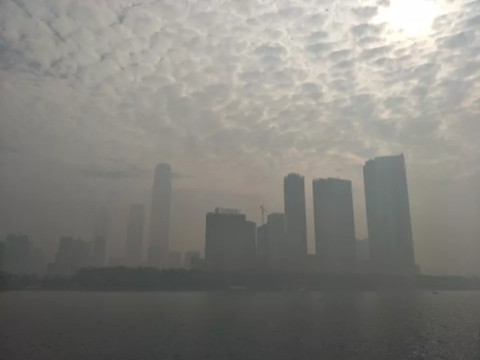
\includegraphics[width=6.67in]{images/cw1}

有人说发展的问题会在发展中解决,例如发达国家也经历过类似的阶段,但伴随产业转型与法规调控,污染问题都会自然而然地消亡;又有人说虽然城市会被雾霾笼罩,但从统计数据上看居民平均寿命其实比所谓田园风光的乡村更长;还有人说大气污染相比土壤、水还有固废污染都不算严重,只是可见度更高(也就是能见度低)\ldots{}\ldots{}的确,雾霾这个现象背后有着错综复杂的社会经济影响,从不同的角度去看会发现不一样的东西。多一个角度看问题并不会让你过的更好,但至少更明白些。

下面我将给出一些非技术与法规调控的视角,希望对读者理解雾霾以及其他一些环境污染问题能有帮助。

\hypertarget{ux7814ux7a76ux589eux957fux7684ux6781ux9650}{%
\subsection{研究增长的极限}\label{ux7814ux7a76ux589eux957fux7684ux6781ux9650}}

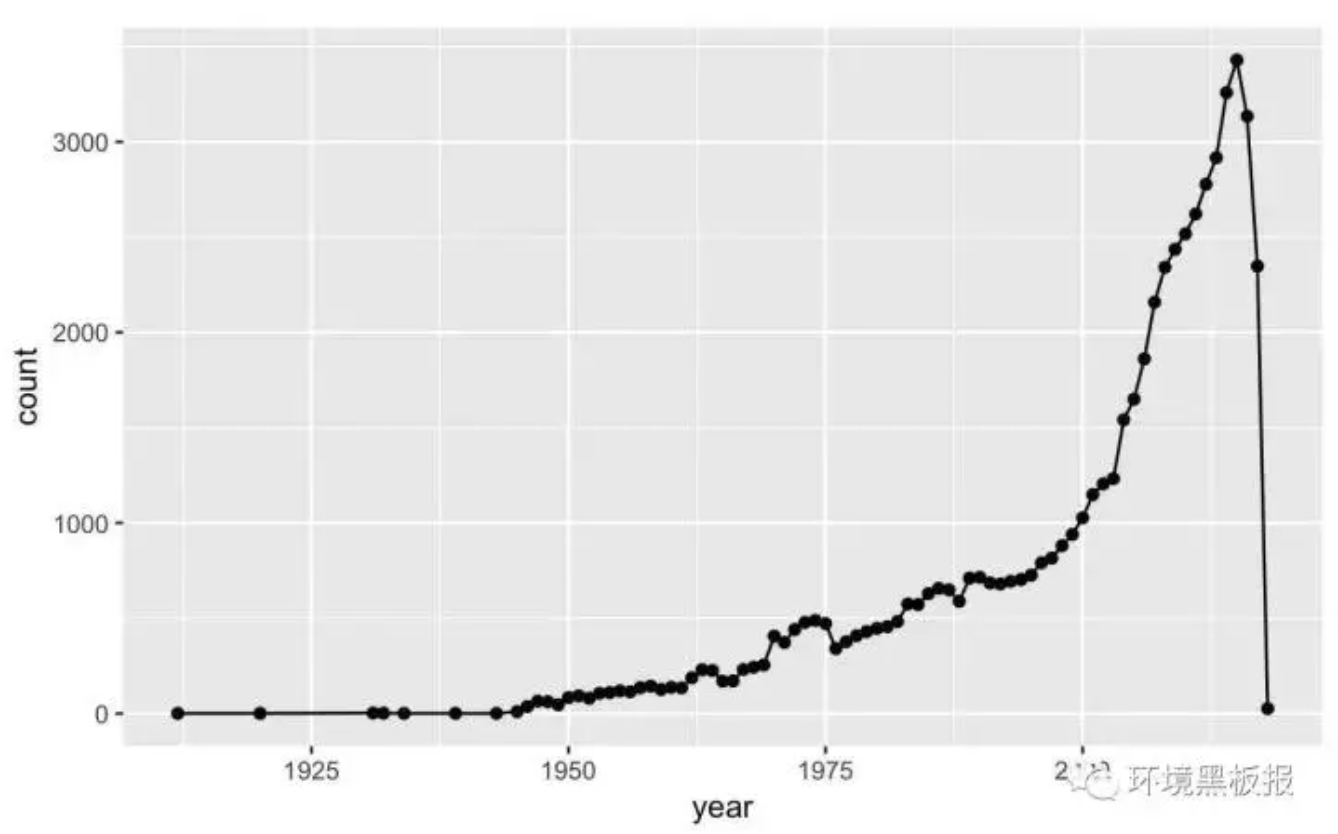
\includegraphics[width=6.67in]{images/cw2}

上图是生物资讯数据库 Pubmed 上用颗粒物(particulate matter)作为关键词得到的论文数量,一百年来可以说是持续增长,特别是21世纪以来增长尤为迅猛。但需要注意的是到2015年达到了峰值(3429),16年已经明显下降(3134),今年还有两个月(2348),但不出意外也不会超过16年。至于为什么会有少量18年文献(26),这是学术界硬通货论文的通货膨胀,透支未来可以说是现代社会最伟大也最危险的发明,学术界亦然。也就是说,对于颗粒物的研究兴趣实际已经在降低了。

这个现象可能有点反直觉,因为近几年大气环境污染的公众关注度非常高,经费投放也很可观,但学术界却降低了学术交流频次。无独有偶,使用传统研究热点例如汞、铬、二恶英、基因组、纳米颗粒去进行检索,都会发现研究在2014-2015年间出现了峰值。但同时如果去看一些新兴研究例如3D打印,颗粒物中的细颗粒物(fine particulate matter),则增长还是非常迅速的(下图是以细颗粒物为关键词的文献发表状况)。

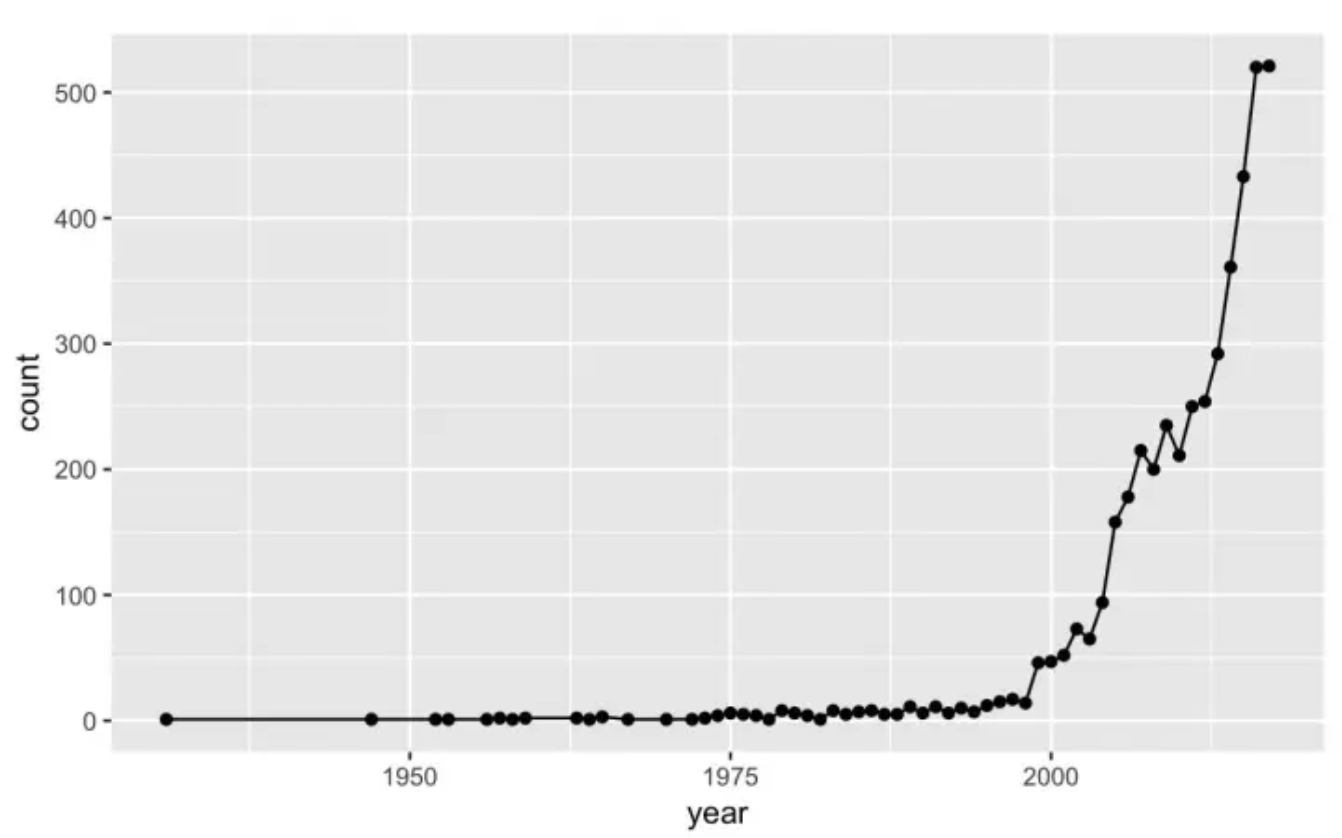
\includegraphics[width=6.67in]{images/cw3}

如果把学术界所有人的研究精力看成是总量稳定的,那么论文数可以看成精力的指标,对于包括大气颗粒物在内的很多环境研究课题而言,学术界正在把蛋糕切给更新的技术与概念。同样是进行雾霾研究,如果你从事微米尺度研究,而学术界却更加认可纳米尺度的研究,那么你的文章就很难发表,然后就是经费紧张,如此循环;进而使得新概念也不断变成老概念。

就颗粒物研究而言,目前学术圈总体关注度已经在下降,但分支中却有上升的。那么可想而知,学科内存在激烈竞争,并不是所有的颗粒物研究方向都是热点。而且还可以预期的是少数研究方向的异军突起会吸收更多学科内的研究资源,很多优秀的研究人员可能一开始选错了研究方向,最终的结局就是转行。研究的增长极限是客观存在的,所以如果你在这个年代打算去找专家咨询,最好去问上升期的新人,因为很多概念从出现到流行不到三五年,有经验的专家反而可能因为有学科内竞争关系而给出带有其自己都意识不到的感情色彩的论断。

\hypertarget{ux6709ux539fux7f6aux7684ux96feux973e}{%
\subsection{有原罪的雾霾}\label{ux6709ux539fux7f6aux7684ux96feux973e}}

如果某天PM2.5爆表,然后你又恰好感觉到嗓子不舒服,那么很自然你会认为这是雾霾的锅。这符合情理,但不一定符合事实,雾霾跟健康是有联系的,但跟健康有联系的可不仅仅是雾霾。即使仅仅考虑大气污染,颗粒物也只是能够产生爆表AQI的一个因素,其余的例如工业主导的硫酸型烟雾或汽车尾气主导的光化学烟雾都会影响健康,都能让嗓子不舒服,此时你会把原因归到哪里?

进一步讲,环境因素也只是影响健康的一个方面,遗传也起作用。假如你在雾霾天听到一个有气管炎家族病史的患者在咳嗽,你会认为是环境影响还是遗传作用?而根据最近Science的一份研究,即便你排除掉环境因素与遗传因素,仅仅是新陈代谢过程中DNA的复制次数就可解释癌症的发病率的66\%,而这个过程根本就无法用先天后天因素来解释,就是个生长问题。

在中国,雾霾是有原罪的,它实际承载了社会转型期人们的一部分焦虑。如果其对健康的总影响是十,那么其中真实作用可能也就二三,替遗传和其他污染物背了三四的锅,还有三四则可以说是心因性的。今年柳叶刀上一篇文献就提到,中国PM1跟PM2.5大概贡献了医院急诊的4.47\%与5.05\%。这种研究有两个问题,第一,即使排除了意外导致的急诊(例如车祸),就诊行为本身就会受天气影响;此外就是 type M 型错误(效应数量级错误),也就是说这个效应是真实的,但是影响不一定大。

这其实是目前环境研究的一个通病,找一组病人和一组正常人(有的连这个也省了)采集样本,然后一把测定几百上千种污染物(这个现在技术上是没问题的),然后算相关系数,这种情况随机你都可以发现几个的,而这样做出的发现有个通病,那就是效应通常不大,很难重现。一个小而真实的效应或许有学术价值,但舆论一放大就会产生公众心理焦虑,而心理状态又会影响生理状态,这类影响可能并不比真实影响小。

雾霾是有原罪的,但被过度聚焦了,由此产生的焦虑与恐慌本身也会产生健康影响。如果公众可以更好理解科学研究现状与其中的问题,这并不能客观降低空气污染的健康影响,但在实际意义上却可能减轻雾霾的心因性副作用。

\hypertarget{ux4e07ux91d1ux6cb9ux7684ux5e7bux8c61}{%
\subsection{万金油的幻象}\label{ux4e07ux91d1ux6cb9ux7684ux5e7bux8c61}}

不知道从什么时候开始,万金油的心态重新出现了。以前如果我告诉你有一种方法可以让你永远远离雾霾危险,你肯定说我瞎扯。好,现在我换一种说法,在人工智能+区块链+可穿戴设备+大数据的实时监控下,我可以给你一副智能眼镜,上面会实时反应你现在的风险指数,如果指数超过80\%,那么你就应该进入室内。逻辑上来说,如果你按照超过指标就躲到室内,那么这个风险永远不会变成100\%,也就是说,这跟我刚才说的永远远离雾霾危险实质等同,但是这样的产品你多半不会觉得是瞎扯,甚至会愿意付高价购买,这又是为什么?

万金油思维从来都没远离过我们,只是从熟悉的名词变成了看似专业的术语。人们有一种看起来很理性但又很荒谬的行为:乐观而盲目地相信着未知的科技。雾霾来了,那就买个最好的空气净化器;外面看不见了,那就来个3M口罩;嗓子不舒服了,那就去搞点清肺的保健品。其实很多人都知道这些科技可能还不成熟,但只要花钱了就有种事情完结可以甩锅的想法。真实的情况往往是越是大家关注的事物,就越有人去贩卖这种包装过的万金油,你买到的更多只是一个确定性的心态。

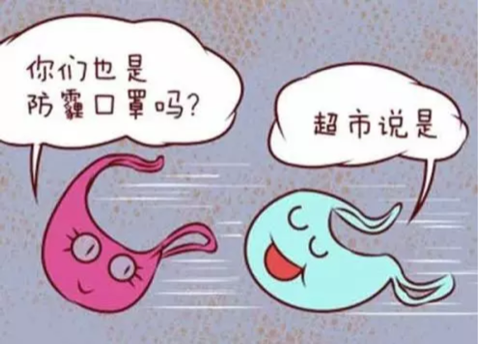
\includegraphics[width=6.67in]{images/cw4}

在这个分工细致的现代社会里,绝大多数的服务业出售的都是经过专业化包装的确定性,用来抵消分工后一颗颗螺丝钉无法感知全局的焦虑。雾霾就是个全局问题,涉及很多不同专业的知识,当个体被复杂性搞晕时,最简单的方法就是掏出一把钞票买个心安理得。即使问题不能在当前根本解决,但生活总要继续,或许这就是万金油思维在进化上的意义。在雾霾这种大IP下,科学家、政府、骗子、掮客、投机商你方唱罢我登场,过分认真你就输了。

\hypertarget{ux6df7ux6c8cux7684ux51acux65e5-1}{%
\subsection{混沌的冬日}\label{ux6df7ux6c8cux7684ux51acux65e5-1}}

回溯千年,宋代诗人陆游在《秋霁》中提到:``驱除云雾极知难'',除了难在技术与法规,雾霾也是直指人心的。

看看窗外,凛冬将至


\includegraphics[width=6.67in]{images/cw5}

作者:yufree
编辑:栟

\hypertarget{ux5317ux4eacux7684ux7a7aux6c14ux53d8ux597dux4e86ux4f46ux662f}{%
\section{北京的空气变好了,但是\ldots{}\ldots{}}\label{ux5317ux4eacux7684ux7a7aux6c14ux53d8ux597dux4e86ux4f46ux662f}}

早在2009年,美国驻华大使馆便自设空气监测站,并对外发布PM2.5数据。而直到2011年以后,随着微博、微信等自媒体的蓬勃发展,一些微博大V、微信公众号开始关注并转发美国驻华大使馆的空气监测数据。这引发了公众强烈热议,什么是PM2.5也成为一时关注焦点,环保等相关政府管理部门也不得不对此有所回应。2013年,国务院发布《大气污染防治行动计划》(就是所谓的``大气十条''),提出十条具体措施,明确经过五年努力,全国空气质量总体改善。而北京随后制定了《2013-2017年清洁空气行动计划》,明确了到2017年底PM2.5年均浓度控制在60微克/立方米左右的``京60''目标。

------写在最初

今年,是``大气十条''的收官之年,北京市空气质量是否明显好转?``京60''的目标是否已经实现?带着这些问题,我们采访了北京某环境监测部门的工程师及中科院某所大气环境研究人员,并对北京市市民进行了街访。

\hypertarget{ux5317ux4eacux7684ux7a7aux6c14ux8d28ux91cfux5230ux5e95ux53d8ux597dux4e86ux6ca1ux6709}{%
\subsection{北京的空气质量到底变好了没有?}\label{ux5317ux4eacux7684ux7a7aux6c14ux8d28ux91cfux5230ux5e95ux53d8ux597dux4e86ux6ca1ux6709}}

北京某环境监测部门工程师(以下简称``监测部门''):从总体上来看,北京市空气质量呈现逐年转好的态势。以PM2.5为例,自2013年开展监测以来,2013-2016年PM2.5年平均浓度分别为89.5、85.9、80.6和73.0微克/立方米,下降的趋势非常明显。

根据北京市环保局发布的监测数据显示,2017年1-10月份,北京市PM2.5累计浓度为64微克/立方米,同比下降8.6\%;空气质量达标,也就是我们所说的``1级优''或``2级良''天数172天,同比增加11天。这些数据均体现了北京市空气质量正逐年好转的特征。

下图是2013年1月-2017年10月北京市PM2.5日平均浓度的热度图(单位:微克/立方米),我们可以看出,这几年,PM2.5高浓度天数确实在减少,低浓度天数在增加。

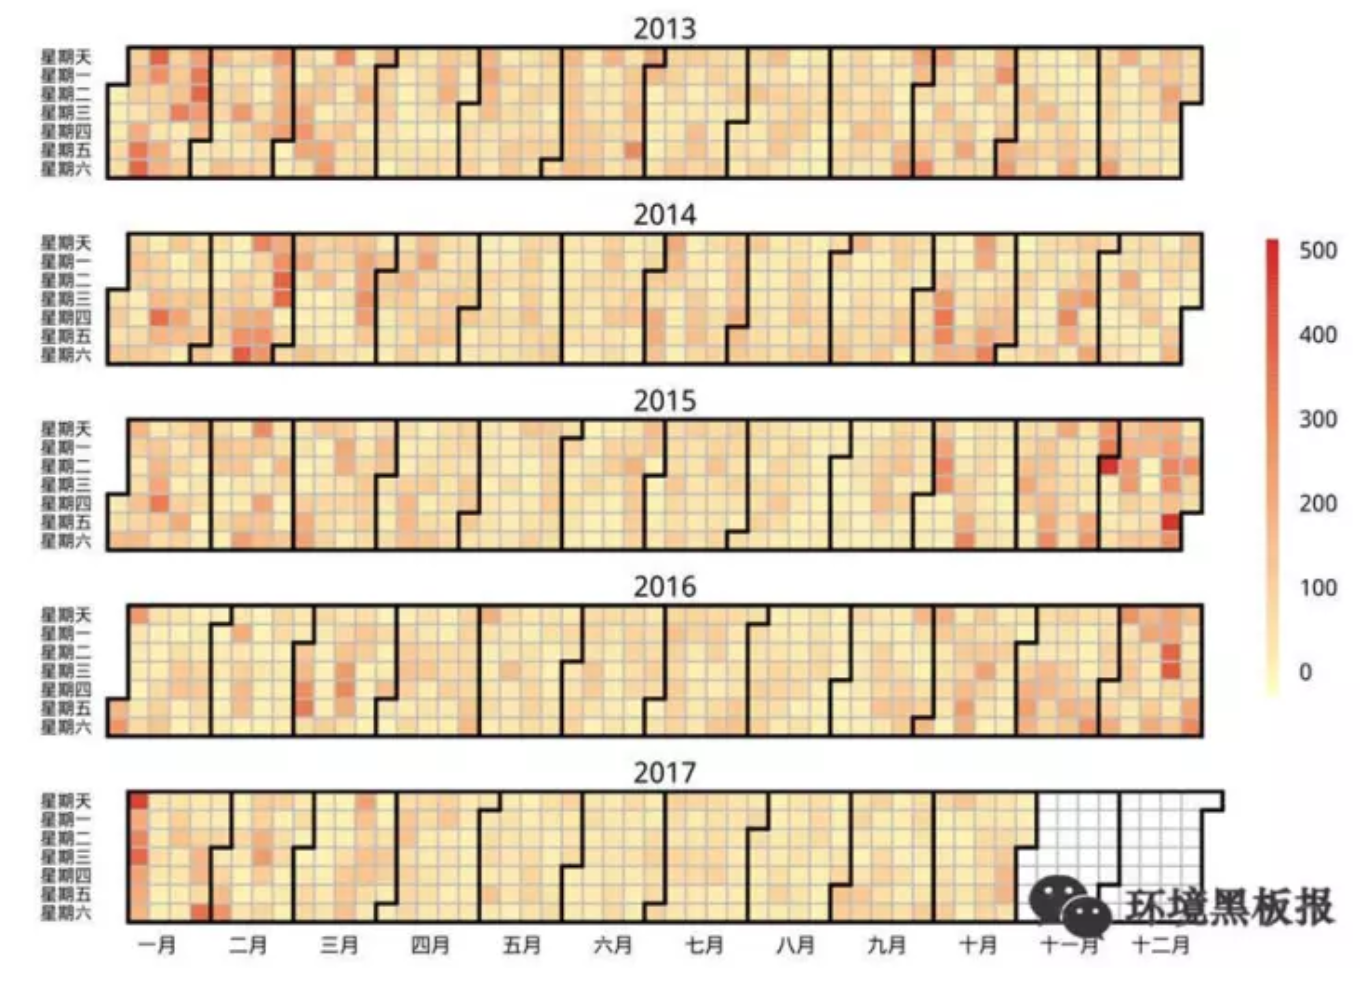
\includegraphics[width=8.33in]{images/air1}

中科院某所大气环境研究人员(以下简称``科研所''):空气质量变好还是变坏,污染物的浓度水平是一方面,污染物的成分变化更需要我们的关注。

举例来说,在1998年,北京主要遭受严重的燃煤和机动车排放混合型污染。自1998至2013年的15年期间,我们国家主要在燃煤电厂的脱硫脱硝技术方面做了很大的改进,使酸雨问题得到了控制。

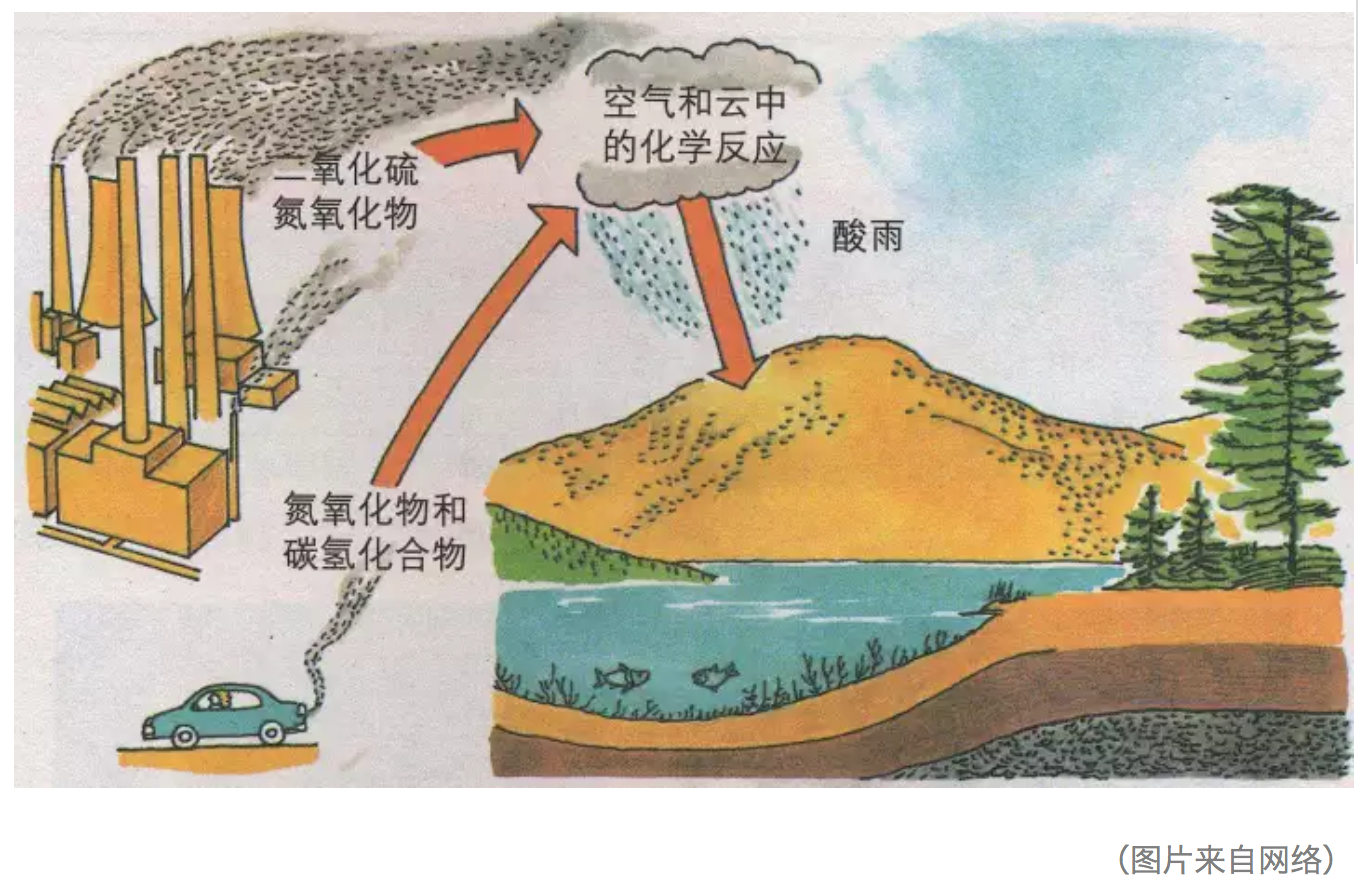
\includegraphics[width=8.33in]{images/air2}

而且,这15年期间,北京的CO、SO2、NO2和PM10的年均浓度均有显著下降,下降比例分别为58\%,78\%,24\%和42\%,尤其是CO和SO2基本稳定在国家空气质量标准值内。

但是,为什么最近几年,雾霾的问题反而更严重了呢?高效的除尘工艺只对粒径大颗粒物具有良好的去除效果,对于数量浓度较高的细小颗粒物去除率还有待提升。尤其在高湿环境下,大气中的多种污染组分如NOx、O3和光照条件促进SO2和VOC等的均相和非均相反应,促进新粒子的生成及细粒子的老化,形成成分复杂的较高浓度的细颗粒物(PM2.5)飘散在空气中,可由呼吸道直接吸入肺部,增大对人体的危害程度。同时,这些细小的颗粒物对阳光的吸收散射增强,降低大气能见度。

这几年随着环保力度加大,尤其是``大气十条''的落实,京津冀、长三角、珠三角PM2.5的浓度比2013年同期分别下降了38.2\%、31.7\%、25.6\%,下降幅度均大幅高于考核标准。``京60''目标也有望实现。

近几年,VOC的排放呈显著增长趋势,或许会成为未来大气污染治理的又一难点。

小编言:随着我们环保治理力度的不断加大,北京空气中PM2.5确实在不断减少,蓝天的数量在不断增加,我们政府下了大决心,打了场胜仗,但是空气质量是否真的变好了,可能还有待研究。

\hypertarget{ux76eeux524dux5bf9ux4e8epm2.5ux6d53ux5ea6ux8bc4ux4ef7ux7684ux6807ux51c6ux4f7fux7528ux7684ux90fdux662fux5747ux503cux59822017ux5e74ux5317ux4eacux5e74ux5747ux503cux8fbeux523060ux5faeux514bux6bcfux7acbux65b9ux7c73ux5de6ux53f3ux8fd9ux6837ux8bbeux7f6eux662fux5426ux5408ux7406}{%
\subsection{目前,对于PM2.5浓度评价的标准使用的都是均值,如2017年,北京年均值达到60微克每/立方米左右,这样设置是否合理?}\label{ux76eeux524dux5bf9ux4e8epm2.5ux6d53ux5ea6ux8bc4ux4ef7ux7684ux6807ux51c6ux4f7fux7528ux7684ux90fdux662fux5747ux503cux59822017ux5e74ux5317ux4eacux5e74ux5747ux503cux8fbeux523060ux5faeux514bux6bcfux7acbux65b9ux7c73ux5de6ux53f3ux8fd9ux6837ux8bbeux7f6eux662fux5426ux5408ux7406}}

监测部门:目前的标准,使用的是均值,每日空气质量评价参考的是日均值,年度目标的完成情况参考年均值。各行各业很多和实际生产生活相关的标准都不需要特别精细化,虽然说设立置信区间能够更精细化,但是在当前的实践中可能比较有难度。标准就是个标尺作用,要满足大部分需要,在满足日常需求上,我认为用均值就够了。不过科学的标准更应该是根据人体健康效应来设置。

科研所:我不认为均值是一个很好的统计量,打个比方,如果只用一个标准值去衡量,那就相当于默认均值背后的分布或者污染特征是一样的,但实际数据的分布并不一样。如果能够精细化一些,可能会更加准确,说服力也更强一些。当然,这也是当前科研出现危机的一个例子,现实的复杂并不适合用简单统计量来描述。

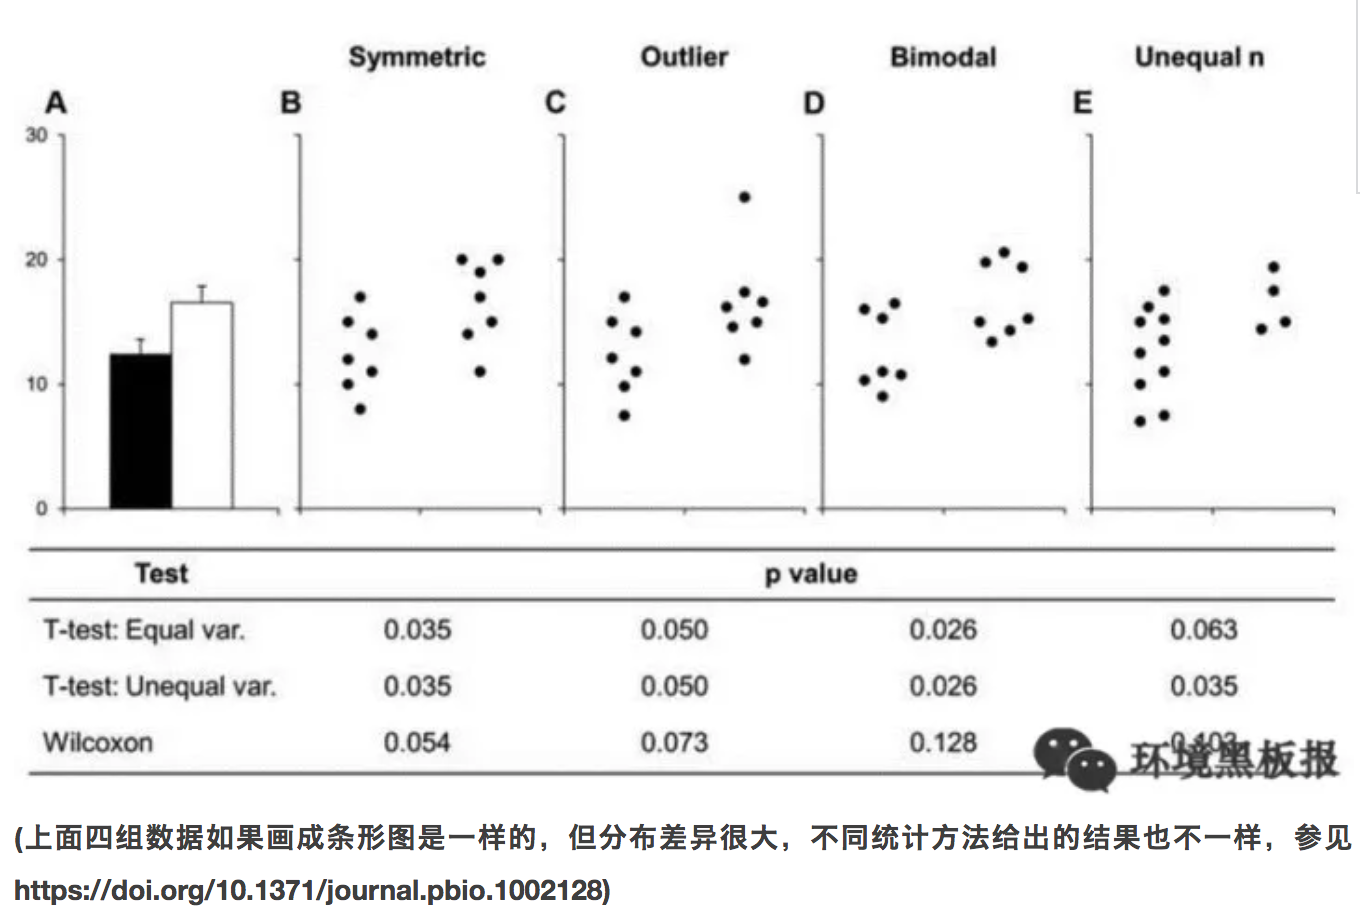
\includegraphics[width=8.33in]{images/air3}

现在环境监测能力越来越强,获得的数据越来越丰富,加上越来越先进的数据处理手段,有实现精细化展示的可能性。标准的制定最好通过置信区间来定义,例如考核指标改为90\%的分时浓度区间,也可以考虑工作日与双休日制定标准。

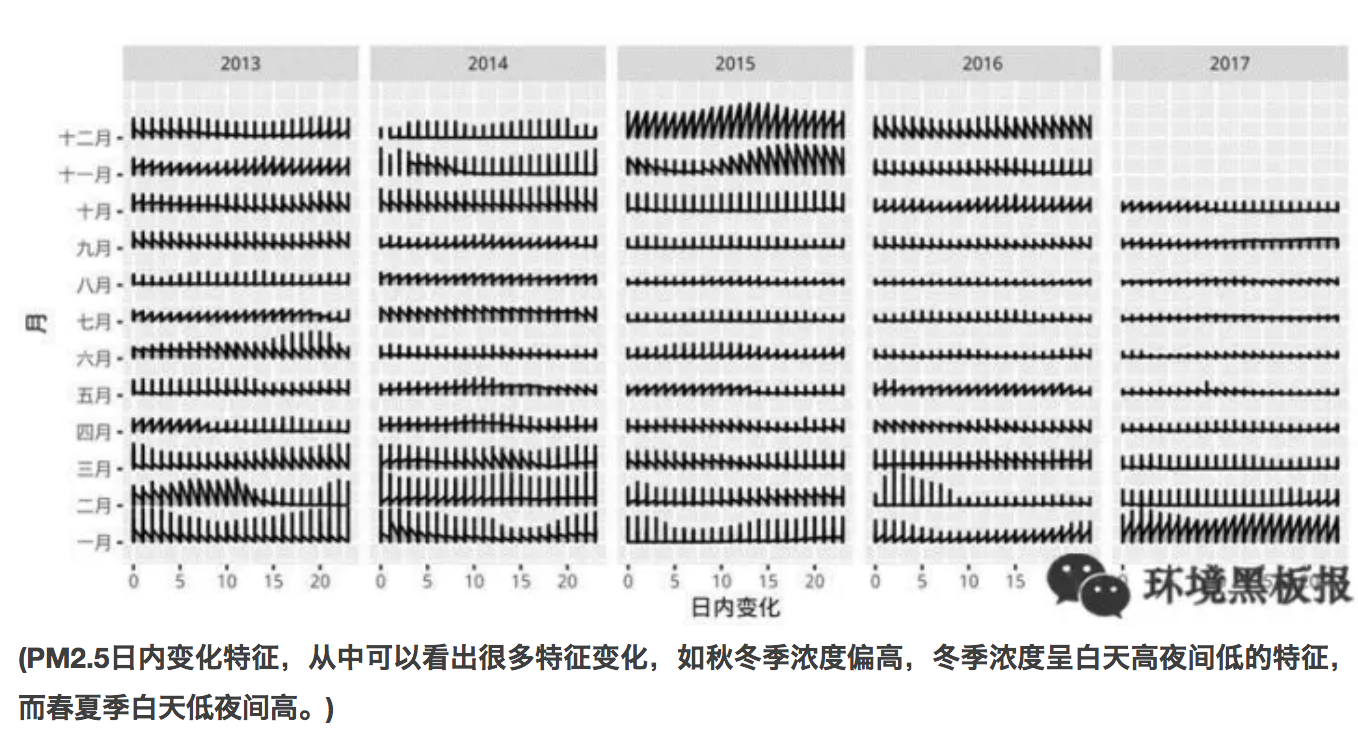
\includegraphics[width=8.33in]{images/air4}

小编言:均值作为标准,应用和管理起来或许会很方便,但是会隐含一些我们看不到的分布特征,而这些特征对于精细化管理大有裨益。

\hypertarget{ux6309ux7167ux5317ux4eacux57ceux5e02ux603bux4f53ux89c4ux52122016-2035ux5e74ux8981ux6c42ux52302020ux5e74pm2.5ux6d53ux5ea6ux4e0bux964dux523056ux5faeux514bux7acbux65b9ux7c73ux5de6ux53f3ux5bf9ux6b64ux60a8ux6301ux4f55ux79cdux6001ux5ea6ux5224ux65adux4f9dux636e}{%
\subsection{按照《北京城市总体规划》(2016-2035年)要求,到2020年PM2.5浓度下降到56微克/立方米左右,对此,您持何种态度,判断依据?}\label{ux6309ux7167ux5317ux4eacux57ceux5e02ux603bux4f53ux89c4ux52122016-2035ux5e74ux8981ux6c42ux52302020ux5e74pm2.5ux6d53ux5ea6ux4e0bux964dux523056ux5faeux514bux7acbux65b9ux7c73ux5de6ux53f3ux5bf9ux6b64ux60a8ux6301ux4f55ux79cdux6001ux5ea6ux5224ux65adux4f9dux636e}}

监测部门:我对此还是持乐观态度的,主要原因为:(1)目前的高压态势环保治理已经成为常态,而不是部分时期采取的临时措施,污染源减排力度将会持续加大。(2)国家正积极加大能源结构调整,目前清洁能源的使用率和使用范围越来越大。(3)民众的环保意识越来越强,自身参与环保的行动也越来越多。在政府和民众的不懈努力下,北京市PM2.5浓度会越来越低。

科研所:对于这个观点,我持乐观态度。首先,政府、民众都很关心,科研人员也在污染源解析、气象模式预报、大气污染追因等方面做了很多的研究工作。其次,治理污染需要一个过程,在2015年以前,重点在酸雨的调控,近几年,重点在PM2.5的调控,未来还有VOC和O3问题也需要解决。根据目前的数据和政府的决心来看,我是持乐观态度的。

小编言:对于未来,我们多是持乐观态度,一方面我们对现在的政府充满了信心,``绿水青山就是金山银山''理论正在引领新实践,另一方面我们自身也深感美丽生活环境的重要性,环保意识不断增强。

听了政府监测部门和科研机构人员的回答,我们已经感受到了政府和研究机构在改善北京空气质量方面所做的努力。那么作为北京市居住的老百姓,作为空气质量改善的最直接受益人,他们的感受是怎么样的呢?

\hypertarget{ux60a8ux597dux60a8ux89c9ux5f97ux5317ux4eacux7684ux7a7aux6c14ux53d8ux597dux4e86ux5417}{%
\subsection{您好,您觉得北京的空气变好了吗?}\label{ux60a8ux597dux60a8ux89c9ux5f97ux5317ux4eacux7684ux7a7aux6c14ux53d8ux597dux4e86ux5417}}

蓝天:感觉今年蓝天确实比去年多了,是不是跟今年风多有关系啊。不过也听说最近环保搞的力度挺大,又是督察又是巡查的,空气污染严重还问责,今年还轰轰烈烈的搞了煤改气,听说周边农村里煤不让烧,气供不上,挨冻了都,好在听说环保部紧急发文,让一些没改好的地方接着烧煤。今年天儿好可能这些治理法子还是起了作用吧。

白云:感觉今年重雾霾好像是好了一点,以前雾霾严重的时候,窗户外面都几乎看不见。其实我对雾霾真是没怎么关注,感觉对自己影响不大,主要是考虑到孩子,希望每天都可以看到蓝天,这几年的雾霾让人有些麻木了吧,到哪里看到雾霾都不觉得吃惊了,反而连续出现蓝天倒是觉得不可思议。

青山:这个我还真关注了,毕竟跟咱北京人儿息息相关么。北京现在空气肯定是在慢慢变好,但是大家感觉不强烈。感觉政府宣传的不好,一方面是老百姓不信,另一方面政府没有转变思维,还是封堵,而不是疏通,预警措施也不够。

\hypertarget{ux6309ux7167ux76eeux524dux5317ux4eacux5e02ux73afux4fddux5c40ux7f51ux7ad9ux516cux5e03ux6570ux636eux5317ux4eacux5e02ux4ecaux5e74ux5f88ux6709ux53efux80fdux8fbeux5230ux5e74ux5747ux503c60ux5faeux514bux6bcfux7acbux65b9ux7c73ux5de6ux53f3ux5317ux4eacux5e02ux7a7aux6c14ux8d28ux91cfux9010ux5e74ux6539ux5584ux60a8ux5bf9ux6b64ux600eux4e48ux770b}{%
\subsection{按照目前北京市环保局网站公布数据,北京市今年很有可能达到年均值60微克每立方米左右,北京市空气质量逐年改善,您对此怎么看?}\label{ux6309ux7167ux76eeux524dux5317ux4eacux5e02ux73afux4fddux5c40ux7f51ux7ad9ux516cux5e03ux6570ux636eux5317ux4eacux5e02ux4ecaux5e74ux5f88ux6709ux53efux80fdux8fbeux5230ux5e74ux5747ux503c60ux5faeux514bux6bcfux7acbux65b9ux7c73ux5de6ux53f3ux5317ux4eacux5e02ux7a7aux6c14ux8d28ux91cfux9010ux5e74ux6539ux5584ux60a8ux5bf9ux6b64ux600eux4e48ux770b}}

绿水:其实吧,我不清楚60微克是啥概念,天天听人说,也没有人科普过,如果说就是雾霾好一点,今年感觉是比去年强点,但要说强多少,也没有吧,前两天不还雾霾来着。

阳光:达标能怎样,数据可以求平均值的,总共有个30天极其严重,而其他天数全是好的,一平均不就是好了,但是老百姓的感官还是不好的。

鲜花:恩,现在政府抓环境抓的紧,我们那片好几个小工地都关了。政府立了指标,老百姓就好监督嘛。而且现在市长是搞环境出来的,又是从环保部过来的,我觉得在改善北京空气方面,还是能有所作为的。

小编言:看来,民众的感受也是因人而异啊,不过总的来说,政府的努力还是得到了认可,民众提出质疑的同时也对政府对科研部门寄予了厚望。

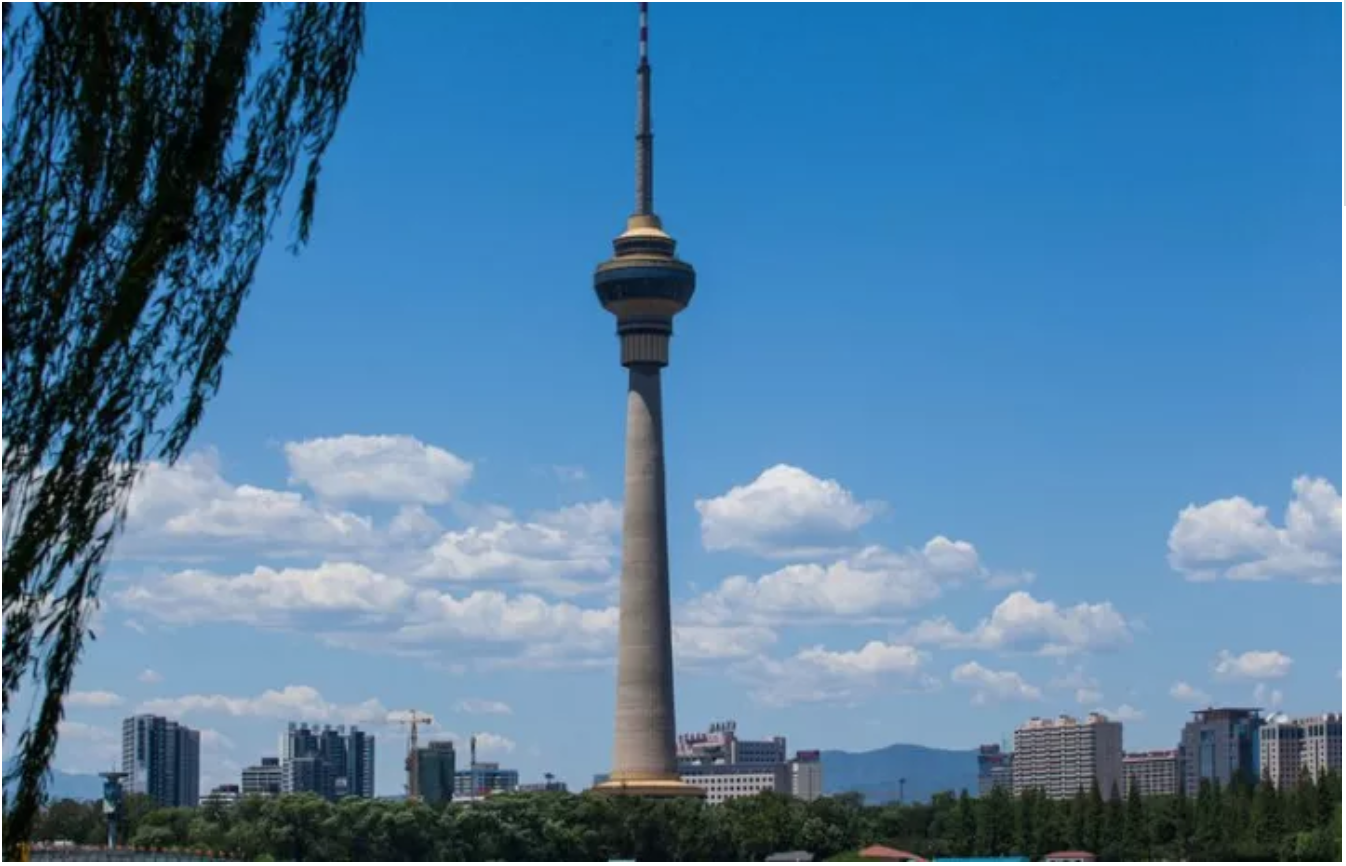
\includegraphics[width=8.33in]{images/air5}

经过几年的努力,北京的空气改善明显,但是否有新形式的污染物出现危害公众健康,是否在目前认为的质量改善背后隐藏着其他的隐患,作为政府工作人员还是科研工作者亦或是你我,都仍需负重前行,不忘初心。

作者: 次要男主角
校稿:周宁,王小咖
图片:yufree
编辑:竹而乐

\hypertarget{ux7b49ux98ceux6765}{%
\section{等风来}\label{ux7b49ux98ceux6765}}

2000年左右,北京人讨厌风,因为一到大风季节,黄沙滚滚,遮天蔽日。可是近些年来,人们又盼着风,期望风来了,把自己从雾霾中解救出来,一时间``等风来''成了所有人的心声。雾霾和风几乎每年都会在北京的地界干上几场大仗,有时力量悬殊,战争迅速结束;有时势均力敌,展开拉锯战。下面我们详细解析一下双方斗争的形势。

\hypertarget{ux4e0eux96feux973eux7684ux6218ux4e89}{%
\subsection{与雾霾的战争}\label{ux4e0eux96feux973eux7684ux6218ux4e89}}

首先我们将北京全市PM2.5(细颗粒物)日平均浓度高于200微克/立方米、持续时间超过2小时的污染状况定义为一次重污染事件,2013年8月到2014年8月期间,我们共观察到六次重污染事件,分别为2013年10月28日(265.59微克/立方米)、2013年12月8日(202.63微克/立方米)、2014年1月23日(233.71微克/立方米)、2014年2月15日(437.15微克/立方米)、2014年2月26日(337.39微克/立方米)和2014年3月27日(234.32微克/立方米)。我们基于GIS软件,通过克里金差值方法对这六次重污染过程形成和消散过程进行了模拟。

\hypertarget{ux96feux973eux7684ux80dcux5229}{%
\subsection{雾霾的胜利}\label{ux96feux973eux7684ux80dcux5229}}

北京PM2.5重污染事件主要受外源传输影响。从重污染形成的过程看,北京这六次重污染过程中,细颗粒物从北京东南部或者南部,逐渐向城中心和西北部缓慢扩散,最终全城形成重污染(图1)。

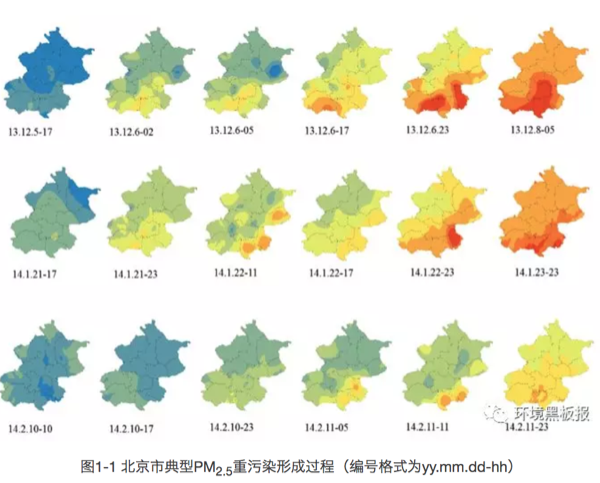
\includegraphics[width=8.33in]{images/windhaze1}

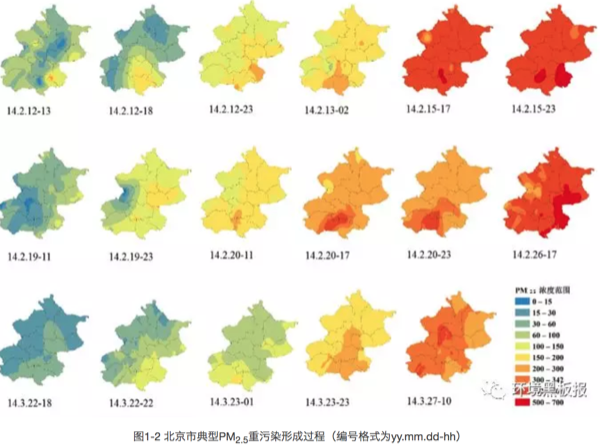
\includegraphics[width=8.33in]{images/windhaze2}

在重污染形成期间北京平均风速低于1米/秒,主导风向为南风和东南风(图2),说明北京的PM2.5重污染的形成受外源传输影响较大。主要的污染物来自北京东南部和南部的廊坊、天津和保定等省市。重污染的形成时间一般为3-7天。

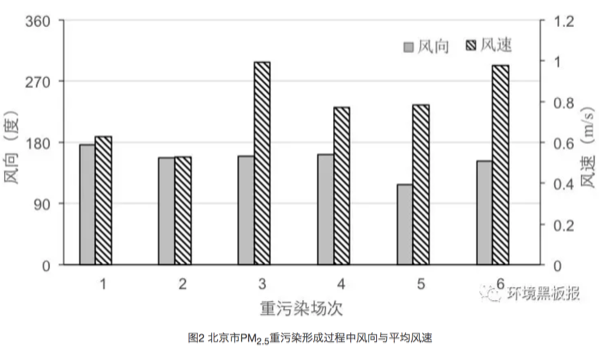
\includegraphics[width=8.33in]{images/windhaze3}

\hypertarget{ux5927ux98ceux7684ux80dcux5229}{%
\subsection{大风的胜利}\label{ux5927ux98ceux7684ux80dcux5229}}

北京PM2.5重污染的消散主要借助风。北京这六次重污染消散过程中,受风的影响,细颗粒物从北京西北部开始,逐渐向城中心和东南部推移,最终实现全城PM2.5消散(图3)。在此期间北京平均风速为2.5米/秒,而主导风向为西北风和北风为主,只有一次为南风。从模拟结果看,北京的细颗粒物被西北风一分为二,之后在向东北和西南逐渐扩散,直至完全消散。说明北京的PM2.5重污染的消散主要依赖于西北风的影响,而且平均风力为2.5米/秒(图4)。重污染的消散过程比较迅速,整个消散过程时间一般在6-11个小时,其中消散最快的一次,出现在2014年2月26日,全市平均PM2.5浓度从431微克/立方米降到21微克/立方米,仅用了6个小时,期间平均风速为3.2 米/秒,主导风向为西北风。其中最慢的一次(2014年2月17日)持续了18个小时。主导风向为东南风,风力2.4米/秒。可见,北京PM2.5的消散过程与风向和风力有密切关系。

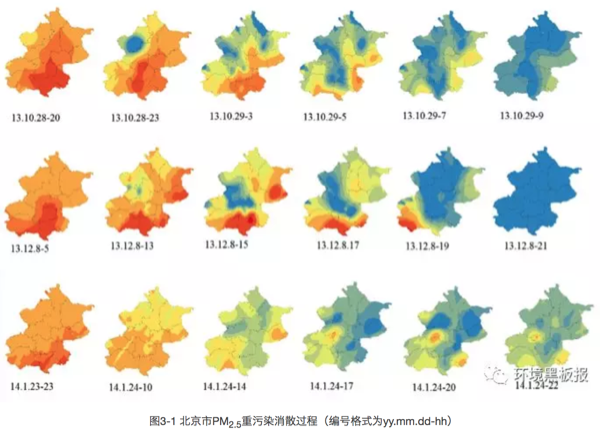
\includegraphics[width=8.33in]{images/windhaze4}

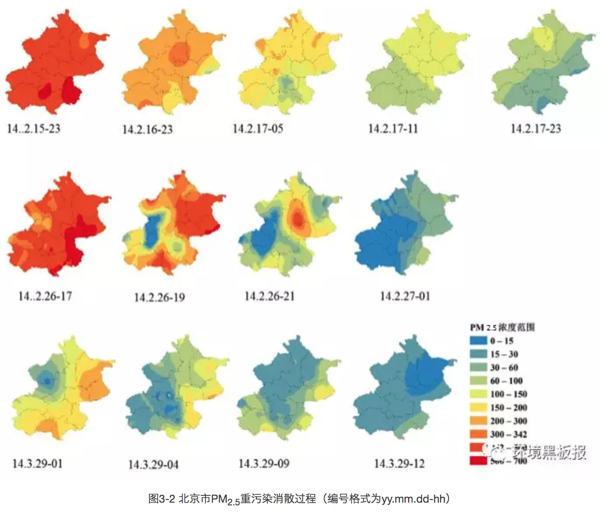
\includegraphics[width=8.33in]{images/windhaze5}

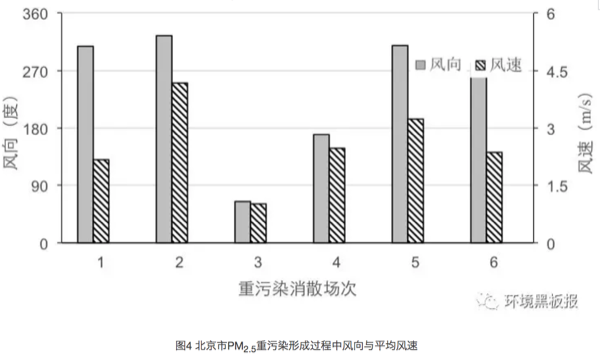
\includegraphics[width=8.33in]{images/windhaze6}

总体看来,风速1米/秒是一个坎,风速小于1米/秒,则容易形成雾霾累积;当风速大于1米/秒,重污染容易扩散,尤其是西北风。

\hypertarget{ux52bfux5747ux529bux654c}{%
\subsection{势均力敌}\label{ux52bfux5747ux529bux654c}}

2018年1月13-17日,京津冀及周边地区经历了一次大范围重污染过程,污染范围包括河北省、山西省、山东省和河南省等城市全部或者部分地区。石家庄市是受重污染影响较大的城市之一,截止到1月21日0时,本次中污染石家庄市出现了164个小时的重度污染和90个小时严重污染(数据来源于网络,未经审核)。

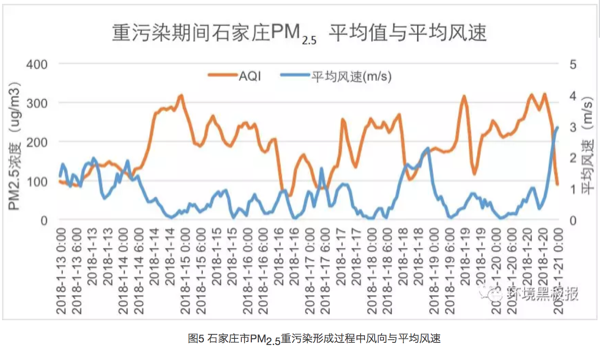
\includegraphics[width=8.33in]{images/windhaze7}

石家庄市从13日凌晨开始空气质量逐步转差,污染物浓度波动上升(图5)。13日5时达到重度污染, 14日6时,污染物逐渐累积,11时达到严重污染。16日14时至17日7时空气质量出现短时改善,部分时段降至中度污染以下水平。此后空气质量继续恶化,重污染持续,但污染程度轻于第一次累积过程。1月18日15时,再次得到短时缓解,之后污染物浓度继续升高,全市PM2.5小时平均值最高值出现在19日12时,达到317微克/立方米。之后迅速下降。1月19日16时,下降到最低值,为117微克/立方米。之后污染物继续累积,1月21日空气质量好转。截止到目前,重污染源已经持续393个小时,其中,有164个小时的重度污染和90个小时严重污染(数据来源于网络,未经审核)。

在此过程中,风速与空气污染指数呈现明显的负相关关系(图5)。风与霾此消彼长,在石家庄市展开拉锯战,持续时间已经超过一周。中间几次过程,主要风速大于1米/秒,空气污染就会得到改善。一旦面临静风时刻,污染物开始逐渐累积。

\hypertarget{ux96feux973eux653bux575aux6e90ux5934ux628aux63a7}{%
\subsection{雾霾攻坚---源头把控}\label{ux96feux973eux653bux575aux6e90ux5934ux628aux63a7}}

在污染治理上,我们要做的还有很多,默默的等风来,不是真正的解决问题的方法。根据贺克斌院士的观点,城市治霾的根本在于管住污染源。2017年8月18日《京津冀及周边地区2017-2018年秋冬季大气污染综合治理攻坚行动方案》(环大气〔2017〕110号)实施以来,在京津冀及周边地区2+26城市,坚持问题导向,把稳固``散乱污''企业及集群综合整治成果和高架源稳定达标排放作为坚守阵地,把压煤减排、提标改造、错峰生产作为主攻方向,把重污染天气妥善应对作为重要突破口,加强联防联控,严格执法监管,强化督察问责,全面实施攻坚行动,动员全民共同应对重污染天气。``攻坚行动''方案规定主要完成的11项任务中有8项与污染源管控有关。截止到2017年12月PM2.5浓度削减幅度最大的前六位城市是石家庄、北京、廊坊、保定、鹤壁和安阳市,与去年同期相比,PM2.5浓度削减幅度均在40\%以上,可见污染源管控才是真正解决雾霾的根本手段。

等风来不如去追风,幸福都是奋斗出来的,总有一天我们能切实做到污染源有效管控,从源头上减少排放,雾霾问题才能从根本上得到解决,相信我们生活的环境会越来越好。

作者:大石
校稿:看透,胜利屯屯长
编辑:丫头晚安

\hypertarget{ux7eb3ux7c73ux975eux7c73}{%
\section{纳米非米}\label{ux7eb3ux7c73ux975eux7c73}}

随着``水十条''、``气十条''和``土十条''的出台,我国已全面启动了``向污染宣战''的环境大战。那么纳米材料如何在环保领域掀起新潮呢?本文以碳纳米材料为一个视角,从选料-制备-应用的角度浅谈一下纳米材料在环保领域如何小试牛刀。

\hypertarget{ux78b3ux7eb3ux7c73ux6750ux6599}{%
\subsection{碳纳米材料}\label{ux78b3ux7eb3ux7c73ux6750ux6599}}

相信在很多读者的印象中,``纳米(Nanometer)''一词总是披着神秘的面纱,影影绰绰,忽远忽近。那么纳米到底是什么?实际上,它与毫米、厘米和分米一样,也就是个长度单位而已,十亿分之一米,即一纳米。

纳米尺度的物质在性质上,跟宏观物体表现出巨大的差异。比如纳米级的金子不再是金色而会失去光泽呈现黑色,纳米级的导电体会变得绝缘,坚硬的金属在纳米级会变得柔软。实际上,无论是人工纳米材料还是天然纳米材料,我们经常与它们亲密接触。大家几乎天天使用的数码电子产品的中央处理器就是用纳米材料制备;iphone的疏油涂层、国家大剧院的穹顶都与纳米材料有关;军事里的隐形战机也是涂了一层吸波纳米材料;甚至大气里的雾霾也包含了各种尺寸的纳米颗粒。可以说纳米材料已经与我们的生活息息相关了。

碳纳米材料的重要性和应用潜力已在最近20年的最高科学奖项中得到承认,包括1996年诺贝尔化学奖(富勒烯)、2008年卡弗里奖(碳纳米管)和2010年诺贝尔物理学奖(石墨烯)。由于其独特的理化性质,碳纳米材料在环境治理领域的应用研究一直是热点之一。然而由于目前的碳纳米材料制备方法成本高、产率低、条件苛刻、生产过程会伴有有毒副产物,极大地限制了其在环境领域的实际应用。因此,迫切需要开发高效、绿色、低成本的材料制备技术。在此背景下,该领域里近年来兴起的``以废治废''新概念逐渐引起了注意。意即将人们通常视作废弃物的材料(如富碳生物质)加工处理成碳材料,再投入到环保相关领域里使用。

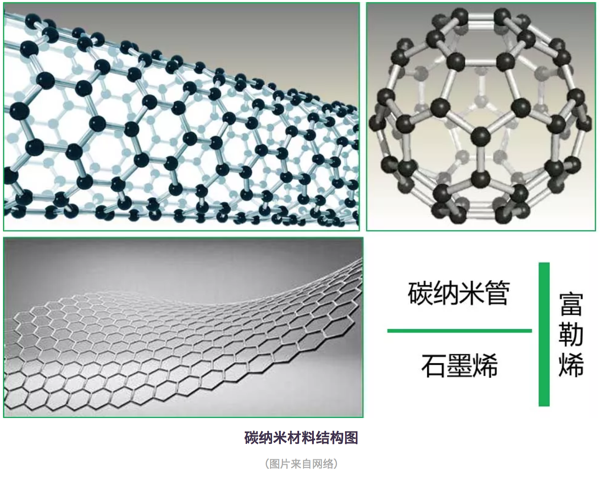
\includegraphics[width=8.33in]{images/nano1}

\hypertarget{ux54eaux4e9bux5e9fux5f03ux7269ux53efux4ee5ux52a0ux5de5ux6210ux7eb3ux7c73ux78b3ux6750ux6599}{%
\subsection{哪些废弃物可以加工成纳米碳材料?}\label{ux54eaux4e9bux5e9fux5f03ux7269ux53efux4ee5ux52a0ux5de5ux6210ux7eb3ux7c73ux78b3ux6750ux6599}}

一般来讲,可以加工成纳米碳材料的废弃物,可以按其环境价值分为两类。一是低值类废弃物。如秸秆、稻草、稻壳等植物类废弃物;动物粪便、剩余污泥等有机质废弃物;以及甘蔗渣、甜菜渣等工业废弃物;二是负值类废弃物,如塑料袋、塑料瓶、海绵、轮胎等。

这两类的大多数废弃物都未得到合理利用,以此类废弃物作为原料制备碳纳米材料,一方面可以降低大规模生产时的成本,另一方面也可解决传统处置方式可能引起的环境污染问题。例如我国农村地区的秸秆(环境黑板报后续会有关于农村秸秆的专题文章)和农膜问题,大量焚烧会造成严重的空气污染和资源浪费。

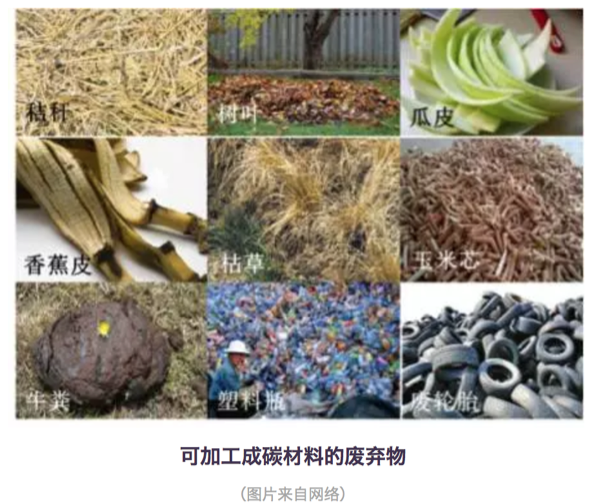
\includegraphics[width=8.33in]{images/nano2}

\hypertarget{ux5982ux4f55ux5c06ux5e9fux5f03ux7269ux52a0ux5de5ux6210ux7eb3ux7c73ux78b3ux6750ux6599}{%
\subsection{如何将废弃物加工成纳米碳材料?}\label{ux5982ux4f55ux5c06ux5e9fux5f03ux7269ux52a0ux5de5ux6210ux7eb3ux7c73ux78b3ux6750ux6599}}

一般有水热碳化法和直接碳化法。

水热碳化法是指在密闭环境中,以水溶液为介质,使原料在高温(100-300°C)高压下经过一系列复杂反应生成碳材料的过程(实际上就是将原料洗好、称好,放铁罐子里扔烘箱里反应半天左右就行)。用水热碳化法制备碳材料,因其操作简单、无污染、对仪器要求低、转化率高等优点被广泛应用。此外,水热法合成的碳材料表面通常会含有丰富的官能团,特别有利于其应用在工业废水的处理中。目前,包括木屑、树叶、稻壳、松针、塑料袋、废报纸等废弃物都被成功地通过水热法碳化成碳材料,还有研究通过此法成功地将草变成了荧光碳量子点。

直接碳化法是指将原料置于无氧条件(惰性气体)下,高温(\textgreater{}600°C)裂解成碳材料的过程。(实际上也很简单,就是将原料放到管式炉中通氮气或者氩气加热一段时间就可以)在高温条件下,原料中的挥发性有机物会逐渐被分解直至留下碳骨架。通常,直接碳化法还需加入一些化学活化剂或者氧化性气体来活化碳材料,以使其表面孔隙度和比表面积增强。碳化温度、升温速率、碳化时间等因素都会影响碳材料最终的形貌和性质。用此法合成的碳材料,表面会具有较强的疏水性,所以对有机污染物的吸附能力很强。

\hypertarget{ux7eb3ux7c73ux78b3ux6750ux6599ux5728ux73afux4fddux9886ux57dfux6709ux54eaux4e9bux7528ux5904}{%
\subsection{纳米碳材料在环保领域有哪些用处?}\label{ux7eb3ux7c73ux78b3ux6750ux6599ux5728ux73afux4fddux9886ux57dfux6709ux54eaux4e9bux7528ux5904}}

\begin{enumerate}
\def\labelenumi{\arabic{enumi}.}
\tightlist
\item
  土壤修复
\end{enumerate}

以废弃生物质制得的碳材料具有发达的孔隙结构,当被添加到土壤中时,可以明显改善土壤结构,降低土壤的体积质量\href{陈心想,耿增超。西北农林科技大学学报(自然科学版),2013,41:\%20167-174.}{1}。另外,生物质以生物质碳材料的形式贮存在土壤中,C元素被固定,减少了向大气的排放;另一方面,生物质碳材料也可以为土壤提供N等营养元素,提升土壤肥力\href{Kezhen\%20Qian,\%20Ajay\%20Kumar,\%20et.al.\%20Renew.\%20and\%20Sustain.\%20Energy\%20Reviews,\%202015,\%2042:\%201055-1064.}{2}。上海交大曹心德教授认为生物质碳材料还可以用于土壤污染物的稳定化修复,他将具有独特吸附性能的碳材料形象比喻为``吸盘'',对土壤中重金属和有机污染物进行吸附``封锁'',从而阻碍植物对污染物的吸收。Puga A. P.等人将甘蔗秸秆制成碳材料用于土壤中重金属钝化研究,发现其可将Cd、Pb 和 Zn 的有效态分别降低 56\%、50\% 和 54\%,并抑制它们向地上部的迁移\href{Puga\%20A\%20P,\%20Abreu\%20C\%20A,\%20et\%20al.\%20J.\%20of\%20Environ.\%20Manage.,\%202015,\%20159:\%2086–93.}{3}。Khan. S.等人使用盆栽试验研究证实, 用污泥制得的碳材料能够减少水稻对As、Co、Cr、Cu、Ni、Pb的吸收\href{Khan\%20S,\%20Cai\%20Chao,\%20et\%20al.\%20Environ.\%20Sci.\%20\&\%20Technol.,\%202013,\%2047\%20:\%208624-8632.}{4}。当然,不同的废弃物原材料、碳化温度、碳化方法制得的碳材料物理化学性质不同,其土壤修复的效果也有差异。

\begin{enumerate}
\def\labelenumi{\arabic{enumi}.}
\setcounter{enumi}{1}
\tightlist
\item
  污水处理
\end{enumerate}

废水中常见的污染物有重金属离子、染料及其他有机污染物。吸附法处理废水由于工艺简单、成本较低、可利用吸附剂来源广泛等优势倍受青睐。废弃物加工制得的碳材料比表面积大、孔隙度高、表面基团丰富,对吸附废水中的污染物十分有利。研究表明,以废弃物为原料制得的碳材料不仅可以通过表面作用(静电吸引、疏水作用、π-π作用等)对重金属离子和有机物分子进行吸附(adsorption),还能凭借较高的孔隙度对油类污染物进行吸收(absorption)。例如新加坡南阳理工大学张华教授课题组成功将废报纸制得碳气溶胶材料用于油类物质和有机溶剂如氯仿等的去除,取得了较好的处理效果\href{Bi\%20H,\%20Huang\%20X,\%20et\%20al.\%20Small\%202014,\%2010,\%203544.}{5},这为解决海洋原油泄露污染提供了一个潜在的解决思路。印度理工学院鲁尔基分校Vinod K.教授将废轮胎制得的碳材料作为吸附剂处理水中重金属离子,发现其对Pb2+、Ni2+有非常好的吸附能力\href{Gupta\%20V\%20K,\%20Ganjali\%20M\%20R,\%20et\%20al.\%20Chemical\%20Engineering\%20Journal,\%202012,\%20197:\%20330.}{6}。陕西师范大学张志琪教授课题组成功将香蕉皮碳化为多空碳材料,发现其对水中典型染料分子亚甲基蓝有较好的吸附去除能力\href{Liu\%20R\%20L,\%20Liu\%20Y,\%20et\%20al.\%20Bioresourse\%20Technology\%202014,\%20154:\%20138.}{7}。

\begin{enumerate}
\def\labelenumi{\arabic{enumi}.}
\setcounter{enumi}{2}
\tightlist
\item
  能源应用
\end{enumerate}

此种碳材料由于较高的石墨化程度,其电子传递能力较强。又由于生物质中还有大量的N,P,S等杂原子,使得由其制备的碳材料导电性进一步增强。因此此种材料在电化学上也具有广阔的应用前景。例如碳材料因为比表面积大、稳定性好、导电性好、价格便宜、来源丰富而成为超级电容器电极材料的首选。我们日常生活中的新能源汽车、数码相机,甚至楼道应急灯都有超级电容器的身影。例如大连理工大学邱介山教授课题组将虾皮制备成氮掺杂碳材料用作超级电容器,其在电流密度为50 mA/g时,比电容可达357 F/g\href{Gao\%20F,Qu\%20J\%20Y,\%20et\%20al.\%20Electrochim.\%20Acta\%202016,\%20190:\%201134.}{8}。利用西瓜皮、麦秸、绿茶、柚子皮、稻壳等制成的碳材料也可作为性能优异的负极材料用于锂离子电池。例如新加坡南洋理工大学于霆教授将竹筷碳化成碳纤维用于锂离子电池,其首次放电和充电质量比容量值分别为500mAh/g和283 mAh/g,且循环稳定性较好,有望替代传统石墨电极在锂电池中的作用\href{Jiang\%20J,\%20Zhu\%20J\%20H,\%20et\%20al.\%20Energy\%20Environ.\%20Sci.\%202014,\%207:\%202670.}{9}。

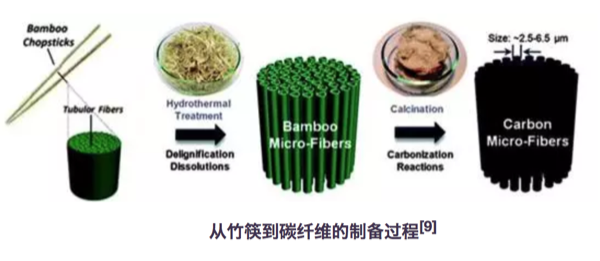
\includegraphics[width=8.33in]{images/nano3}

\hypertarget{ux7ed3ux8bed}{%
\subsection{结语}\label{ux7ed3ux8bed}}

以废弃物为原料制备的碳材料已被广泛研究用于土壤修复、污水处理和电化学领域,展现出了广阔的潜在应用前景。废弃物来源广泛、价格低廉的性质也使得此概念为大规模商业生产提供可能。然而目前对废弃物碳材料的研究才刚刚起步,处于发展阶段,很多碳材料仅限于实验室制备而没有进行大规模的工业化生产,距离大规模实际应用还为时尚早。

此外,在大规模应用之前,其对环境可能造成的潜在风险也有待进一步研究。这也正是纳米科技目前的发展缩影。正如中国科学院院长白春礼所说:``纳米科技发展方兴未艾,基础科学研究领域中新原理不断建立、新功能材料的涌现与可控制备技术的发展、纳米生物医药的应用探索都体现出纳米科技对人类知识体系的极大拓展以及对生活方式的潜在推动作用。尽管纳米材料显示了产业化以及临床应用的巨大前景,但多数材料目前仍处于实验室研究阶段,如何实现这些材料的功能化、推动商业化应用、相关的生态影响和生物效应是纳米科技发展面临的关键问题''。中国科学院生态环境研究中心江桂斌院士曾将基础研究形象比作翻书:``当书本一页一页翻至最后时,就是量变到质变的时候''。这也同样适用于纳米领域,或许质变之时我们就能用上充电几秒即可充满的电子产品,纳米机器人实现药物精准输送、有的放矢。

文献引用

作者:眼神防守
校稿:柴胡半夏苏,yufree
编辑:栟

\hypertarget{ux4f60ux559dux7684ux53efux80fdux662fux6709ux6bd2ux7684ux81eaux6765ux6c34}{%
\section{你喝的可能是``有毒''的自来水?!}\label{ux4f60ux559dux7684ux53efux80fdux662fux6709ux6bd2ux7684ux81eaux6765ux6c34}}

\hypertarget{ux6c34ux53d1ux751fux4e86ux4ec0ux4e48ux6c34ux6c61ux67d3}{%
\subsection{水发生了什么?------水污染}\label{ux6c34ux53d1ux751fux4e86ux4ec0ux4e48ux6c34ux6c61ux67d3}}

地球是个名副其实的``水球'',水资源总储量约为1.36×109km3,但除去海洋等咸水资源外,只有2.5\%为淡水。淡水又主要以冰川和深层地下水的形式存在,储存在河流湖泊中能被人类所利用的淡水仅占全世界总储水量的0.3\%, 然而,这极为稀有的淡水,却面临着另外一个不可忽视的严峻问题------水污染。水污染问题使得人类``获得安全可靠的饮用水''这一基本诉求难上加难。

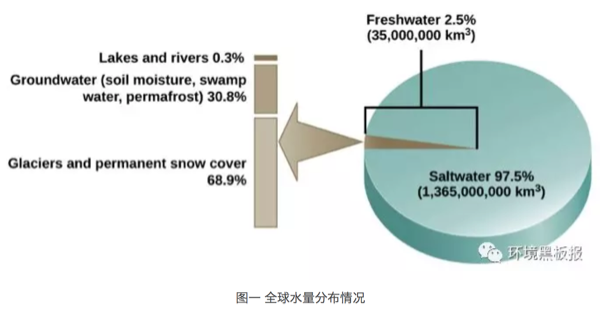
\includegraphics[width=8.33in]{images/dushui1}

联合国组织秘书长在2002年世界水日发布的新闻稿估计, 全世界有11亿人无法获得安全饮用水。中国的水污染问题尤其严重,如图所示,中国绝大部分地区的饮用水仅满足最低标准,在中南部有些地区,饮用水水质更加糟糕。

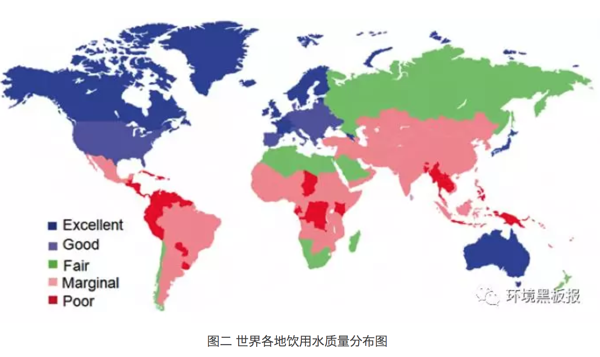
\includegraphics[width=8.33in]{images/dushui2}

\hypertarget{ux5f15ux8d77ux6c34ux6c61ux67d3ux7684ux7f6aux9b41ux7978ux9996ux662fux8c01ux6c61ux67d3ux7269}{%
\subsection{引起水污染的罪魁祸首是谁?------污染物}\label{ux5f15ux8d77ux6c34ux6c61ux67d3ux7684ux7f6aux9b41ux7978ux9996ux662fux8c01ux6c61ux67d3ux7269}}

近些年来,全国各地水污染事件频发,如2012年12月,位于山西省长治市境内的煤化工厂发生苯胺泄漏入河事件,导致河北省邯郸市发生停水和居民抢购瓶装水,同时由于泄漏苯胺已随河水流出省外,河流下游的河南省安阳市境内红旗渠等部分水体亦检出超标的苯胺、挥发酚等污染物。

综合所有水污染事件可得出,引起水污染的污染物有很多,通常可分为三大类,即物理性、化学性和生物性污染物。

物理性污染物包括悬浮物、热污染物和放射性污染物。其中放射性污染物危害最大, 但一般存在于局部地区。化学性污染物包括有机和无机化合物, 该类化合物近些年来在环境水体中频繁被检出。生物性污染物包括细菌、病毒和寄生虫。随着痕量分析技术的发展,至今从源水中检出的化学性污染物已达数千种以上。在所有的化学性污染物中,微量有机污染物逐渐引起人们的广泛关注,并已成为世界几乎所有地区水污染的首要污染物。

微量污染物是指那些广泛使用但通常在很低或者极低浓度水平就能影响自然环境生物化学过程的有机污染物,包括人工化学合成品,比如活性药物成分、食品添加剂、化妆品成分和洗涤剂成分,以及天然存在的一些物质如激素、生物毒素等。近年来,一些新型微量污染物,例如药物与个人护理品(PPCPs)、内分泌干扰物(EDCs)、全氟类化合物(PFCs)等的环境污染及潜在影响问题已成为各国学者和公众关注的焦点。很多微量污染物具有较强的环境持久性、生物活性、生物累积性和难降解性,如果长期暴露于环境中,对生态系统和人类健康将带来难以预测的潜在风险。我国是各类工业品、药品的生产和消耗大国,工业和人口密集,能源和资源利用率仍然较低,高强度的工业化学品生产、使用和废弃会产生严重的环境效应,因此微量污染物的环境残留问题更是不容忽视。

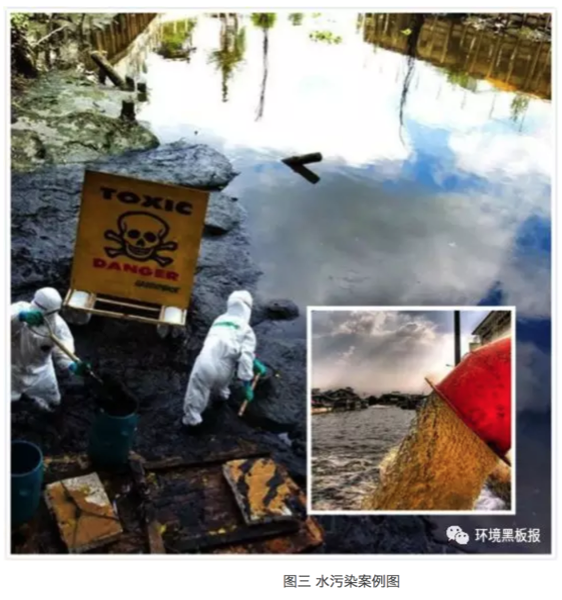
\includegraphics[width=7.81in]{images/dushui3}

\hypertarget{ux6c61ux6c34ux5904ux7406ux5382ux53efux4ee5ux4f7fux6c34ux53d8ux5e72ux51c0ux4e48ux672aux5fc5}{%
\subsection{污水处理厂可以使水变干净么?------未必!}\label{ux6c61ux6c34ux5904ux7406ux5382ux53efux4ee5ux4f7fux6c34ux53d8ux5e72ux51c0ux4e48ux672aux5fc5}}

为了去除环境水体中的微量污染物,人们寄希望于现有的污水处理工艺。然而,当被污染的水经过污水处理厂处理之后,真的可以变干净么?答案却是未必!

\begin{itemize}
\tightlist
\item
  微量污染物的去除很难达到100\%
\end{itemize}

近年来,欧盟和一些发达国家开始高度关注水环境中的微量污染物问题,研究发现城市污水中化学物质普遍存在,有些是常规污水处理工艺难以去除的,因此污水排放是河流水体中化学物质的重要来源。

城镇污水处理厂的工艺选择主要基于排放标准中COD、BOD5、NH3-N、TN、TP等常规污染物指标的稳定达标。另外值得注意的一点是,污水中的许多痕量污染物具有一定的毒性,对活性污泥中的微生物易产生一定的抵抗和抑制作用,因此,目前常用的污水处理工艺如活性污泥等对痕量污染物的去除并不能达到100\%。同时,在污水处理工艺流程中,部分微量污染物通过活性污泥吸附或者生物降解、水解等得到去除,但许多亲水性物质不能吸附到活性污泥上,导致出水仍然残留相对较高的浓度,释放到接纳水体中,引起水生生物的慢性接触。需要关注的是,某些微量污染物具有中等或较强的疏水性,易于被活性污泥絮凝吸附;但由于仅仅是相的转移而不是降解,这部分被吸附的微量污染物往往随着污泥的处理处置过程进入地表水体或土壤环境中,直接或间接造成潜在的环境与健康风险。城镇污水处理厂出水及污泥是环境中不可忽视的痕量有机污染物的源。

\begin{itemize}
\tightlist
\item
  残存的微量污染物可能在处理过程中发生二次反应生成更毒的物质
\end{itemize}

在当前的污水处理厂中,化学降解方法包括光催化氧化,臭氧化和氯化被认为是有效处理微量有机污染物的几种工艺。然而,虽然微量污染物可以在一定程度上被去除,但由于有毒转化产物的生成,使得其环境健康风险却未必消失。有各种报道称,微量污染物在化学降解过程中可能转化成其他的副产物,使得污水处理厂的出水毒性反而较处理之前增加, 这些转化产物最终进入地表水,甚至到达饮用水,对水生环境及人体健康造成更高的生态及健康风险。有研究表明,这些有毒的转化产物可能破坏内分泌干扰系统,干扰人类和动物的激素系统功能。此外,有些有毒转化污染物还可能致癌,致突变和引起生殖系统的病变。例如,在饮用水氯化处理过程中, 有大量的消毒副产物如三卤甲烷,卤乙酸及亚氯酸盐等生成,这些消毒副产物已被证实在较低的剂量下即可以诱发肝癌和肾癌,并可降低精子的自动力,影响生殖系统的发育。

换句话说,人们原本寄希望于去除有毒的微量污染物从而得到干净安全的饮用水,这一目的不仅难以达到,相反,被污染的水在经过污水处理厂处理后可能生成更加有毒的转化产物,使得其环境和健康风险可能更高!更为糟糕的是,民众对于这一现象知之甚少,以为自己饮用的是一杯经过处理之后的干净安全的饮用水,实则却是一杯含有有毒化学物质的``不健康水''!

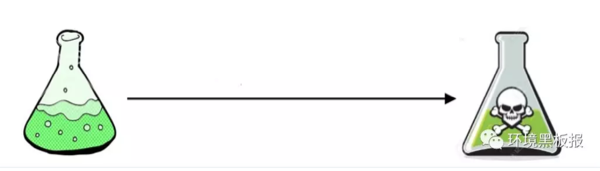
\includegraphics[width=8.33in]{images/dushui4}

\hypertarget{ux5c0fux7ed3}{%
\subsection{小结}\label{ux5c0fux7ed3}}

中国约50\%的水源受到微量有机化合物及重金属离子等物质的污染,令人堪忧的是,目前全国县以上4000多家自来水厂中,95\%以上仍然使用传统水处理工艺,这些工艺在处理有机化合物及重金属离子时,处理效果并不理想,同时,即使这些传统处理工艺能够在一定程度上去除该类污染物,更加有毒的转化产物也可能会生成使得自来水面临更高的健康风险,而普通民众对于这一事实却无处知晓。

水污染问题的确是个相当棘手的大问题,利益关系错综复杂,要完全改善也并非一朝一夕,是一个缓慢长远的过程! 笔者认为目前的水污染治理还存在诸多问题,首先,水质检测不够专业认真。几乎所有的饮用水专家和学者都认为中国的水质存在严重的安全隐患,但是在众多自来水厂的报告中,却几乎没有一家自来水厂自检水质不合格。这一看似矛盾的现象说明很多自来水厂在水质检测上并不认真,很多时候仅是马马虎虎测一些无关痛痒的参数告知民众自来水是安全的,但是背后真正的问题并没有被揭示出来。其次,污染控制不严,执法力度不够。自来水水质优,首先应得益于严格的水源控制。为保障水源安全,应建立水源保护区,在保护地带内,禁止一切有污染物质的进入,违者应被加以重罚。但我国目前的情况却是,许多工厂非法排污造成水源污染,但是当民众给所属环保部门报告时,监管部门大多并未作出积极的反应,或者即使作出反应,也仅是隔靴搔痒,并未真正杜绝该类地下排污问题的发生。

2015年``水十条''落地,预示着政府将握紧拳头向水污染宣战,笔者真心希望政府在以上问题上加大监管力度,对故意排污造成水污染的当事者予以重罚,同时对环保部门及水质检测部门加以规范,以期对水质状况获得最真实的第一手数据,为日后的水污染治理提供重要的观测基础。

作为与水息息相关的我们每一个人,除了等待政府可以更快更好的解决水污染问题,在日常用水中时要及时观察生活用水的水质变化,看其是否出现异常颜色或浑浊,有无异物及异味等。饮水前先放水,让水流一会儿,将管道中的``死水''流出再饮用。另外如有条件,建议增加具备反渗透膜过滤的净水器。

作者:李立平(博士,毕业于香港科技大学,从事水处理领域近7年,在相关研究领域发表学术论文数篇)
校稿:yufree,大石
编辑:丫头晚安

\hypertarget{ux4e00ux6ef4ux6c34ux7684ux6545ux4e8b}{%
\section{一滴水的故事}\label{ux4e00ux6ef4ux6c34ux7684ux6545ux4e8b}}

曾几何时,一滴水随着千万个同伴出现在这个星球。他们开始塑造这个星球,改变着地貌,孕育着生命。人类从出现的那一刻起,就开始了与水相爱相杀的历史。从两河流域的空中花园到尼罗河流域的金字塔,从马拉松的烽火到牧野之战的硝烟,水,孕育了地球最初的文明。同时,人类早先的传说,从诺亚方舟到大禹治水,又无处不在昭示着人类对水的敬畏。

水与人类的相爱相杀一直在进行着。有一滴水躲在茶壶里变成了蒸汽,告诉一位叫瓦特的人这样的力量可以推动机器运转,于是推动了轰轰烈烈的工业革命;有一滴水和同伴们一起构成了江、河、湖、海,让人类可以物流南北、货往东西,文明的火种得以靠水传播。

人类使用着水,也污染着水;净水养育着人类的同时,污水却时刻威胁着人类,这样的相爱想杀更是直接催生了我们的专业------环境科学与工程。此刻我们对水充满敬畏,毕竟水撑起了整个产业链上的勤劳的人们。水进入大气在不利的气象条件和污染物参与的情况下,形成雾霾,这一点我们在《混沌的冬日》里已经写过;水进入城市,若无法正常下渗、排除,则形成内涝,这直接催生了海绵城市的建设思路,这一点我们在《城市之殇》中已经展现;即使不听话的、因污染而变坏的水,工程师们不死心,坚信每一滴水都是清纯的,于是我们人类建立了污水处理厂,通过活性污泥法和生物膜法等工艺,使受污染的水改头换面,还清还纯,而这在《污师私房菜》中,我们也有所提及。

地球的水储量是巨大的,然而淡水资源却是如此的稀缺,环境工程师们在累死累活守护净水的同时,一个``开源''的灵感开启了水资源的另一段神奇之旅:

\hypertarget{ux6d77ux6c34ux6de1ux5316}{%
\subsection{海水淡化}\label{ux6d77ux6c34ux6de1ux5316}}

海水淡化方法主要分为热法和膜法。

热法:海水的盐度很高,直接饮用只会越喝越齁,但早在公元前1400年,海边的居民便学会了在锅内把海水加热到沸腾,使海水蒸发变成水蒸汽,盐分留在锅底成为垢,并使水蒸汽遇冷成为可饮用的蒸馏水。这也是今天常用的蒸馏法海水淡化的原型。而现代常用的热法海水淡化主要有多级闪蒸和低温多效两种。

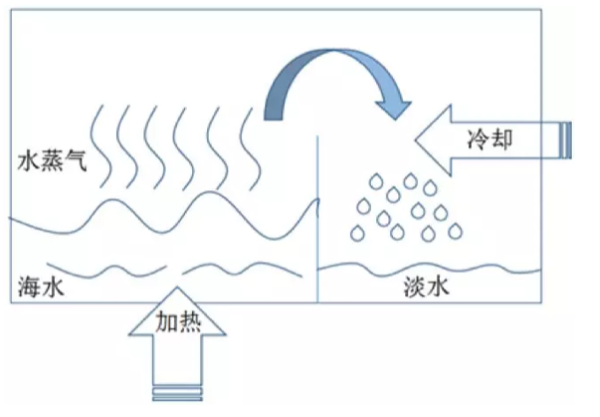
\includegraphics[width=8.33in]{images/seawater1}

膜法:1950年美国佛里达大学瑞德(C.E.Reid)教授在无意间发现了一个奇怪的现象。他观察到海鸥在海上飞行时从海面啜起一大口海水,隔了几秒后,吐出一小口海水,这个现象引起了他的思考。后来经研究发现,海鸥体内有一层薄膜,该薄膜非常精密,海水被海鸥吸入体内后,经过压力作用使水分子穿透薄膜转化为淡水,而含有杂质及高浓缩盐分的海水则吐出嘴外。于是,受此启发,瑞德教授提出了反渗透的基本理论。反渗透膜如同一只特殊的过滤筛子,在压力下过滤掉了水,而留下了盐(看到这里我觉得瑞德教授至少不是一个喜欢吃野味的人)。运用这一原理,我们就可以利用反渗透膜从盐水中获取淡水了。

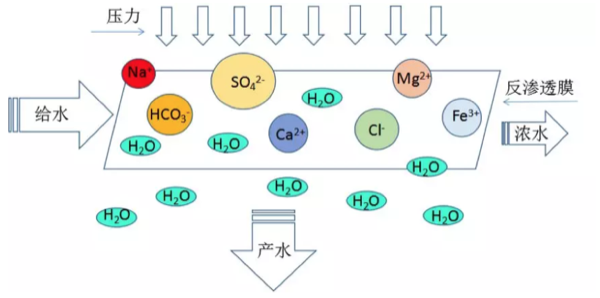
\includegraphics[width=8.33in]{images/seawater2}

我国人口占世界22\%,淡水占有量却仅为8\%,世界排序名列109位,是世界上12个严重贫水的国家之一。而海洋中蕴藏着丰富的淡水,其总量约占海水的97\%,相当于13.3亿立方公里之多,是一个巨大而又稳定的淡水储库。海水淡化作为水资源的开源增量技术,具有稳定供水、应急供水和战略性供水的特点,是解决沿海水资源短缺问题的重要途径。笔者收集了我国沿海地区人均水资源情况,发现沿海地区由于经济发展水平和人口密度较高,缺水情况反而高于全国平均水平,形成了靠水没水的情况。海水淡化成为了一些沿海地区解决缺水问题的关键手段之一。

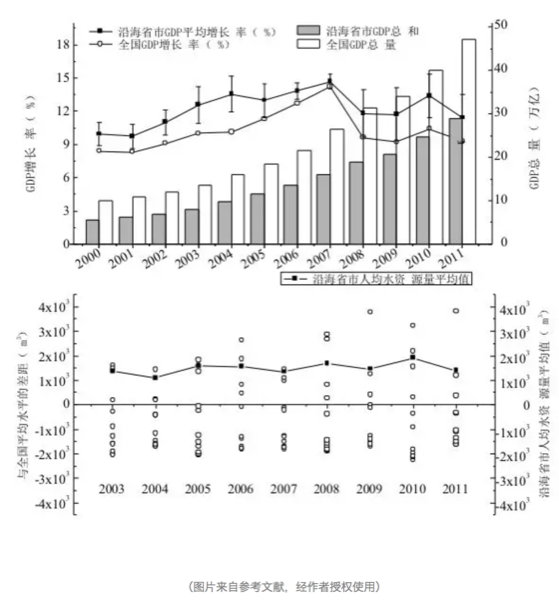
\includegraphics[width=7.76in]{images/seawater3}

我国海水淡化的历史始于上世纪五十年代。至2015年,全国总产能已经超过百万吨,约为全球海水淡化总产能的2\%左右。随着经济的发展,我国在国际海水淡化市场的比重逐渐增加。如下图所示,我国在这一年的产能增长约为中东地区的一半左右。中东地区存在一些自然条件上的限制,促使他们更加积极地开发海水淡化技术,因此中东地区历来是海水淡化最重要的市场,所以我们国家海水淡化产能比不过这些土豪真的不丢人。

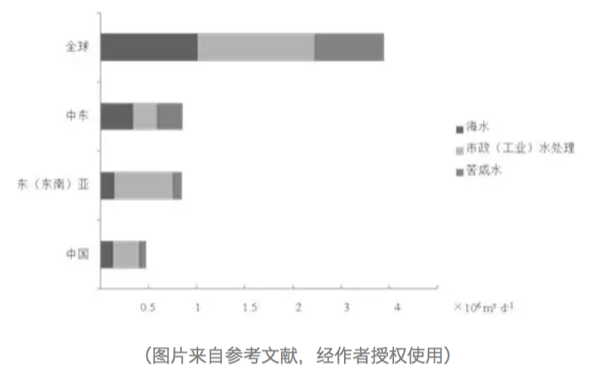
\includegraphics[width=8.33in]{images/seawater4}

目前我国已建的海水淡化产能主要集中在辽宁、天津、河北、山东等北方省市,这四省市产能占我国海水淡化总产能的81.9\%(2014年数据,见下表);与此对应的是不同省份对于海水淡化的关注度,下图是来自海水淡化的网络搜索指数,排行前五分别是北京、广州、浙江、江苏、山东,从中不难看出,海水淡化的关注度和接受水平也与地区的经济发展状况息息相关。

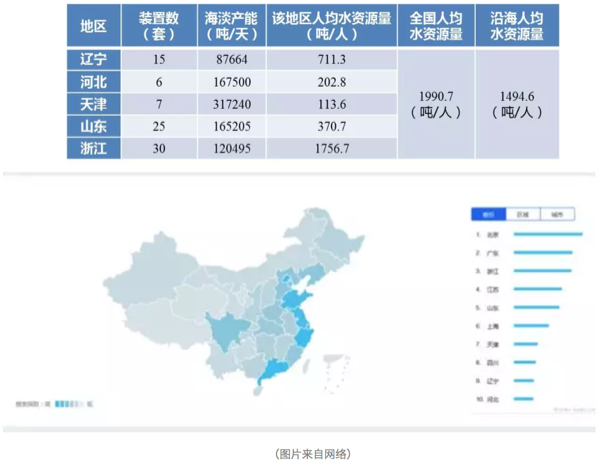
\includegraphics[width=8.33in]{images/seawater5}

2016年12月,国家发改委和国家海洋局联合印发的《全国海水利用``十三五''规划》指出,到``十三五''末,全国海水淡化总规模拟达到220 万吨/天以上,其中沿海城市新增海水淡化规模105 万吨/天以上,海岛地区新增海水淡化规模14 万吨/天以上。而海水直接利用规模拟达到1400 亿吨/年以上,海水循环冷却规模达到200 万吨/小时以上。新增苦咸水淡化规模达到100 万吨/日以上。海水淡化装备自主创新率达到80\%及以上,自主技术国内市场占有率达到70\%以上,国际市场占有率提升10\%。相信未来海水淡化会有更快的发展。海水淡化项目在某种程度上是一种基础建设项目,与各级政府的施政方向密不可分,所以虽然国家出台了一系列的规划政策,具体落地还是需要很长一段路。

\hypertarget{ux540eux8bb0}{%
\subsection{后记}\label{ux540eux8bb0}}

2010年,我们像一个一个水滴汇入了中科院这个汪洋大海,拥有了这片汪洋大海里的化学物质。随着时间的推移,我们又流到了其他地方,在各自的岗位上吸收了新的化学物质。不同物质间的反应总能产生新的物质,所以我们决定讲我们的源,讲述我们每一滴水的故事。

作者:yy
校稿:胜利屯支书,看透
编辑:栟

\hypertarget{ux5c0fux79f8ux79c6ux5927ux95eeux9898}{%
\section{小秸秆,大问题}\label{ux5c0fux79f8ux79c6ux5927ux95eeux9898}}

2017年11月,演员孙艺洲拍戏途径哈尔滨,被郊县烧秸秆的烟熏味儿呛到流泪,随后在微博上抱怨:为什么一个白天空气质量优良的城市到了夜晚就空气爆表?为什么?怎么办?这个问题并不算新,但当它被一个拥有一千多万粉丝的耿直boy问出来的时候,还是结结实实触到了很多人的痛处。

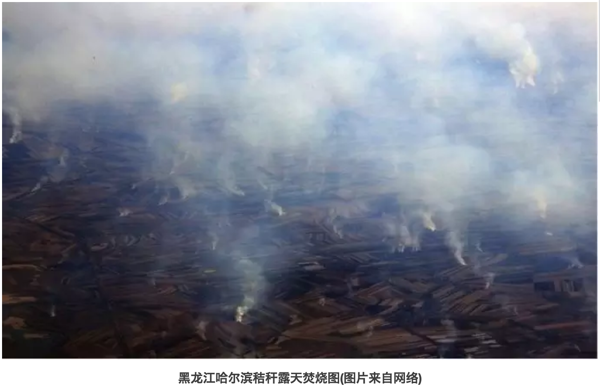
\includegraphics[width=8.33in]{images/stalk1}

在哈尔滨,把孙艺洲呛到流泪的是秸秆焚烧产生的颗粒物。每年秋收以后,庄稼被打捆、加工、再被送到每个人的餐桌上,算是完成了自己的历史使命;但秸秆这种副产品却被留了下来。

在田间地头,常常可见成垛的玉米或者小麦秸秆,勤快点儿的农户,将其垛得整整齐齐,也算是道风景;懒一些的,堆放得毫无章法,影响观瞻。

其实这个时候农民是真的忙。每年10-11月,是我国 ``秋收秋种''期,各级农业部门一级战备、高度紧张,密切关注天气变化和降雨量,一轮又一轮的``紧急通知'',为的是指导农民收得时机合适,种得不早不晚。因为只有这样才能保证丰产丰收。

我们大东北黑土地在这个时候是收玉米种小麦,秋收整地追求``深、净、细、实'',小麦播种要在适宜播种期抢播早播。收下来的玉米秸秆无处可放,尽管我国80年代起就出台各种秸秆禁烧的相关规定,禁烧态势越压越重,但比起秸秆处理的经济压力和劳动力需求,很多农民不由自主就选择用``一把火''解决问题。

不烧不行啊,秸秆太多了。1991年我国秸秆产量为6亿多吨,经过了粮食总产量的``十三连丰'',到2015年,秸秆产量为10亿多吨。多出的秸秆总量为4亿多吨!什么概念呢?如果把这4亿多吨秸秆以100根为一扎首尾相连,能绕地球赤道转325000圈\ldots{}\ldots{}

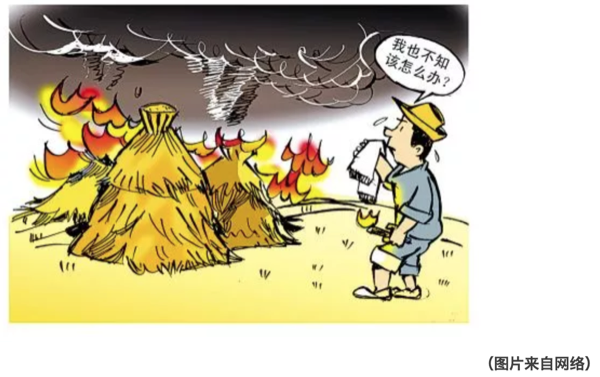
\includegraphics[width=8.33in]{images/stalk2}

不烧不行啊,农民家里实在没人。壮劳力都出去打工了,只剩下老人和孩子,尽管乡里承诺可以集中处理,那也需要把秸秆运输到集中处理点,老人孩子不会开车,没有工具,再好的政策也解不了眼前的急。

但烧秸秆的确是后患无穷。农作物光合作用的产物有一半以上保留在秸秆里,它富含氮、磷、钾、镁和有机质,秸秆大量集中燃烧的过程也是一种剧烈释放能量和物质的过程,周围环境根本无法在短期内消纳这么多的释放物,大气污染因此产生。

跟燃煤锅炉引起的污染不同,秸秆焚烧的主要产物是颗粒物、一氧化碳、二氧化碳等,对城市和乡村的低空空气影响更为直接。然而在大气污染研究领域,秸秆燃烧对雾霾的贡献一直颇有争议。

撇开具体贡献率不谈,稍加研究便可发现:在10月和11月的秋收期,从华北到东北(每年秸秆主要燃烧区),雾霾符合低硫份、高悬浮颗粒物、连片集中爆发的特点。

换句话说,叠加了大规模的秸秆焚烧,使得轻中度采暖季雾霾立刻升级为大范围重度雾霾。环保部10月期间的卫星遥感巡查监测数据分析表明,在16个省(区)共监测到疑似火点1583个,比2014年同期增长74.5\%,也的确证实了秸秆燃烧对雾霾的推波助澜``功效''。

所以,怎么办才好?秸秆问题和我国的大多数农业问题一样,工程浩大、解决起来困难重重。

目前秸秆的综合利用工作虽在稳步推进,但仍存在很大问题:一是秸秆还田成本高,运营公司与农户缺乏主动性;二是农民缺乏必要的技术支持,导致秸秆无法真正实现废物利用。

就东北地区来说,冬季气温偏低,秸秆还田要想充分被土壤消纳,必须使用进口农机深度翻耕,进一步增加了还田成本和土壤压力。说白了,东北地区黑土地耕作土层只有20厘米,想翻耕30厘米好让还田秸秆快速腐烂,需要钱,需要时间,需要人力,需要对新茬农作物减产的心理预期。

与这些困难形成对比的是,政府部门越来越强硬的禁烧手段。自1997年起,我国开始重视秸秆禁烧和综合利用工作,到2008年明确农作物秸秆综合利用分工、确定综合利用比例,再到2014年重拳出击京津冀及周边地区,提出部分地区全部实现秸秆综合利用的目标,禁烧力度越来越大。

进入2015年以后,我国出台了``史上最严''大气污染防治法,明确了县级人民政府应该补贴支持秸秆收储运和综合利用服务,并规定:露天焚烧秸秆的,可以处五百元以上二千元以下的罚款。

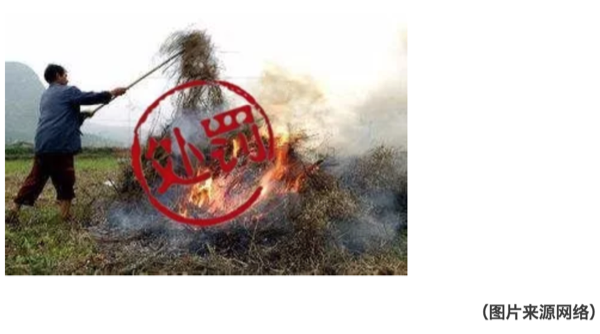
\includegraphics[width=8.33in]{images/stalk3}

为了彻底杜绝火点,在大气污染防治法的框架下,有些省份开出了自己的处罚清单。河南省在增加督查和暗访的基础上,以环保部公布的秸秆焚烧卫星监测火点数为依据,以县(市、区)为单位,出现一个火点,省财政扣拨县(市、区)财政资金50万元,力度之大空前绝后。

秸秆问题逐渐进入人们的视线并得到如此重视,除了它与雾霾之间千丝万缕的联系之外,还因为它的确是农业和环保领域牵一发而动全身的节点。

一根秸秆,一头连着三农,一个敏感脆弱又是万事之本的领域,一头连着环保,一个同样是成长痛点难点的行业。不能烧,但也不能接受粮食减产!粮食减产,根基没了,中国人民要挨饿;烧秸秆,污染加剧,人民叫苦连天。相信很多民生问题都是如此。

好在中国人民是世界上最勤快的人民。纵观其他国家,在面对这个问题的时候农民往往是两手一摊,对执法人员说``我没办法呀!''\ldots{}\ldots{}毫无悔改之意。

美国作为一个重要的粮食输出国,直到2011年在中部和东南部仍有大量火点发现,可比我国东北严重多了,有NASA图为证。印度人民更是开挂,烧着秸秆接受记者采访,大大方方毫不避讳。

秸秆的五料化利用技术(肥料化、饲料化、基料化、燃料化、原料化)并不高深,而秸秆问题的处理方式千差万别,对应效果天壤之别。

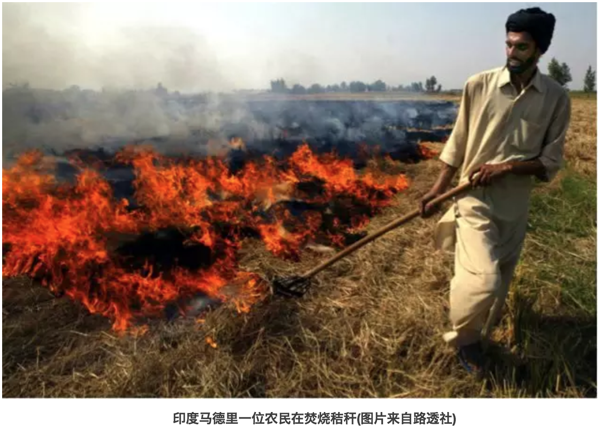
\includegraphics[width=8.33in]{images/stalk4}

解决秸秆问题,一个靠重视,一个靠财政。回看我国,重视程度和经济投入力度都需更进一步。

2007年,美国政府投资1.25亿美元建设了3个生物能源中心,专门进行纤维素生物能源研究。同年,美国农业部出资1400万美元、能源部出资400万美元,共同设立基金研发生物燃料、生物能源及相关产品的研究与开发。

据统计,2008-2012年,美国政府对生物质研发法中涉及的项目共计投资了1.18亿美元。除了对研发环节和支持外,美国对可再生能源发展规定了技术开发抵税和生产抵税的措施,生物质发电和秸秆纤维素乙醇项目都享受响应的税收补贴或者减免。

对比我国,2016年,农财两部门整合资金10亿元,选择秸秆焚烧问题较为突出的10个省份开展秸秆综合利用试点,取得了初步成效。果然真金见实效。

现在秸秆综合利用的主要方法是还田(直接和间接),直燃、气化、制沼,制醇和用作饲料、栽培基料等。

还田的方式简单、粗暴、直接、见效快,被各地采用最多,但由于地域差异明显,也存在一些弊端和后患。

直燃、气化、制沼和制醇等方式都需要大量的经费投入,各省由于财政状况难以统一,无法按照某个标准整体推进;另一方面,秸秆禁烧和综合利用与农户素质密切相关,在加大财政投入的同时,提高农民认识,增强回收利用秸秆的积极性也是较为有效的措施。

而在环境黑板报更新的《纳米非米》中,提出了以秸秆等有机废物为原料制备生物碳材料``以废制废''的观点,也是秸秆处理另一条可选择的路径。

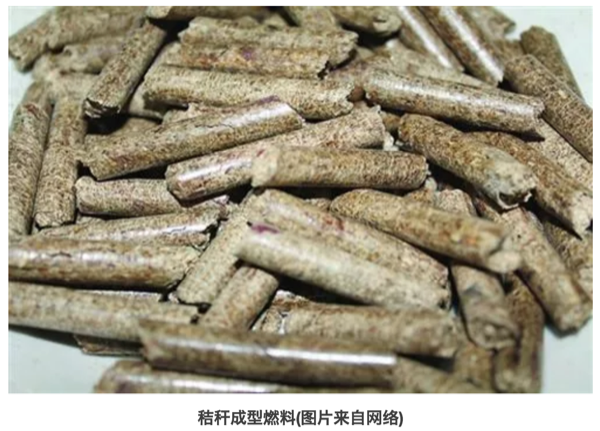
\includegraphics[width=8.33in]{images/stalk5}

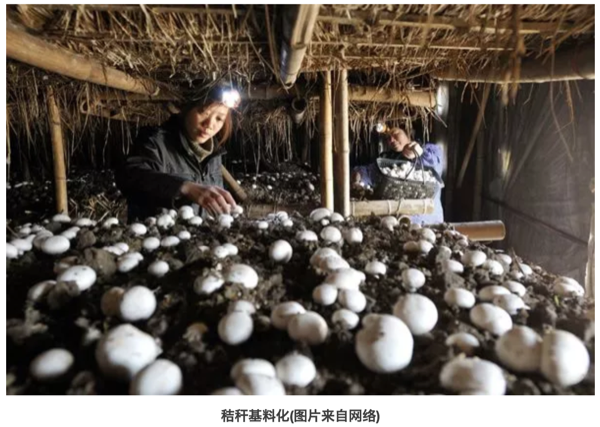
\includegraphics[width=8.33in]{images/stalk6}

\hypertarget{ux7ed3ux8bed-1}{%
\subsection{结语}\label{ux7ed3ux8bed-1}}

据悉,今年11月份哈尔滨火点问题爆出以后,相关责任人已于近日被环保部约谈,东北秸秆问题治理的机遇和挑战也随之而来。秸秆燃烧这种事,连遥感卫星都看得到,还怕执法部门不知道吗?小秸秆、大问题!希望所有的环保责任人能够直面问题,应对挑战。在关注大动向时,不忘记身边还有这样的``小事情''也同样需要我们的努力!

作者:胜利屯支书
校稿:广播站王站长、柴胡半夏苏
编辑:竹而乐

\hypertarget{vocux51cfux6392ux5927ux6c14ux6cbbux7406ux7684ux65b0ux6311ux6218}{%
\section{VOC减排------大气治理的新挑战}\label{vocux51cfux6392ux5927ux6c14ux6cbbux7406ux7684ux65b0ux6311ux6218}}

\hypertarget{ux524dux8a00-1}{%
\subsection{前言}\label{ux524dux8a00-1}}

``今天空气质量怎么样?适不适合户外活动?''关注空气质量已经成了人们日常生活的一部分。由于人口增长和工业及经济的快速发展,人类在生活和生产中向大气中排放的污染物量也日渐增多,主要包括二氧化硫、氮氧化物、烟粉尘等颗粒物、挥发性有机化合物(Volatile organic compounds,VOCs)等等,而由此引发的大气污染问题也层出不穷:除了被热议的灰霾,酸雨、温室效应、光化学烟雾、臭氧层破坏、有毒物质扩散等也不容小觑。随着《大气污染防治行动计划》的实施,我国对二氧化硫、氮氧化物、烟粉尘排放控制取得明显进展,但VOCs防治工作相对滞后。目前,VOCs减排已经成为大气污染防治的重点。VOCs是什么?对于局外人来说,可能非常陌生,但在大气治理的圈子内,它已经火的不要不要了。那么,挥发性有机物到底是何方神物,会引起如此大的关注?

\hypertarget{vocsux662fux4f55ux7269}{%
\subsection{VOCs是何物}\label{vocsux662fux4f55ux7269}}

\hypertarget{vocsux7684ux5b9aux4e49}{%
\subsubsection{VOCs的定义}\label{vocsux7684ux5b9aux4e49}}

学术界对于VOCs的定义是指沸点在50\textasciitilde{}260℃,室温下饱和蒸汽压超过133.32Pa的易挥发性有机化合物。简单点说,挥发性有机物首先是有机物,然后这种有机物容易由液态转为气态物质进入环境空气中。举个例子,装修完之后,很多朋友会关心甲醛的问题。甲醛是胶粘剂的主要成分,板材中残留的和未参与反应的甲醛会逐渐向周围环境释放,甲醛就是生活中最常见的VOC。除了甲醛,生活中接触到的油漆、汽油等都含有VOCs。

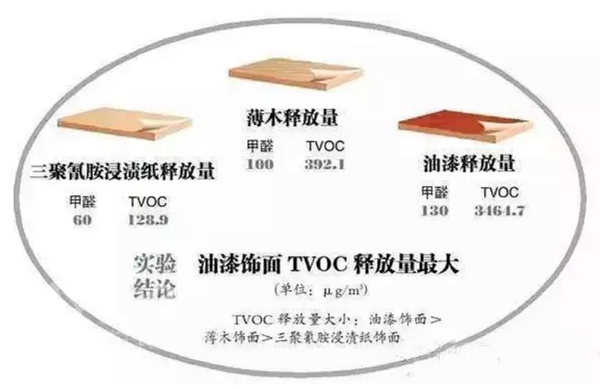
\includegraphics[width=8.33in]{images/voc1}

VOCs之所以被关注、被研究、被减排,就不得不说说它的危害。VOCs不仅危害环境,而且危害身体。一方面,VOCs是大气环境中光化学反应的前体,在阳光照射等特定条件下,会与环境空气中的化学物质,发生一系列光化学反应,生成臭氧,而形成光化学烟雾。同时,VOCs也是灰霾重要的前体物质,通过对细颗粒物(PM2.5)源解析,大气中VOCs在PM2.5中的比重占20\textasciitilde{}30\%,还有部分PM2.5由VOCs转化而来。

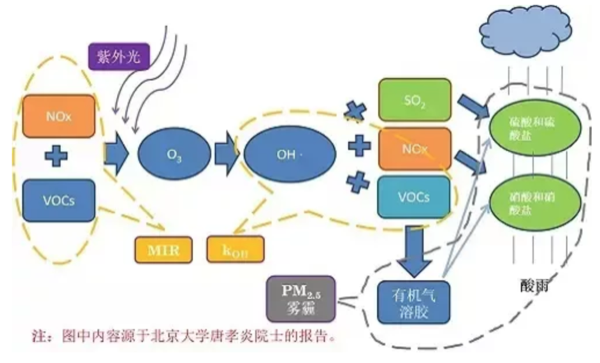
\includegraphics[width=8.33in]{images/voc2}

另一方面,大多数的挥发性有机物均有病理毒性,都对人体各器官组织有较大的危害作用。以甲醛为例,其在室内达到一定浓度,可引起眼红、眼痒、咽喉不适或疼痛等症状。

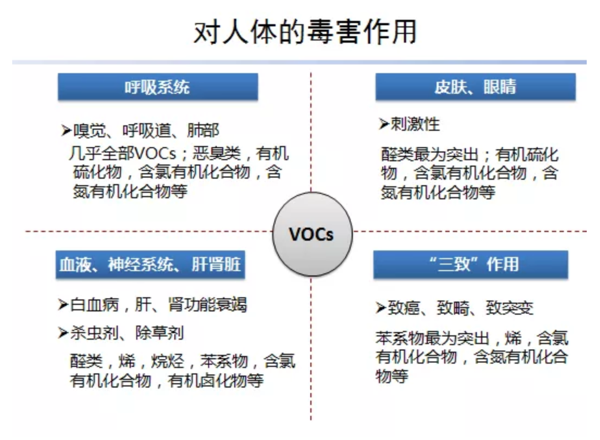
\includegraphics[width=8.33in]{images/voc3}

VOCs排放源主要包括自然源和人为源。自然源主要为植被排放、森林火灾、野生动物排放和湿地厌氧过程等,属自然界的正常规律,源和汇处于平衡状态。而人为源大致可分为工业源、生活源、农业源和移动源。有调查报道,我国VOCs的工业源和交通源为主要的人为源,分别占43\%和28\%。

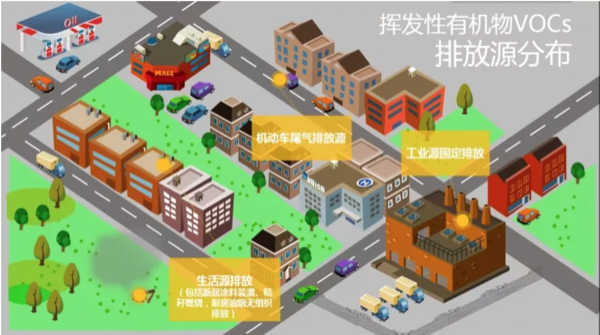
\includegraphics[width=8.33in]{images/voc4}

其中工业源排放企业涉及的行业有电子信息、纺织印染、石油化工、家具、木材加工、塑料橡胶制品加工、包装印刷、制药等,这些行业也正是目前我国主流工业。正因为人类活动,越来越多的VOCs进入大气中,在环境空气中的累积,打破了自然界VOCs源和汇的平衡。

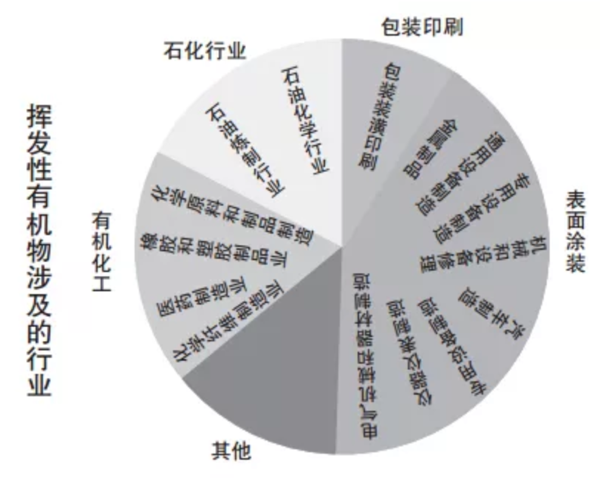
\includegraphics[width=8.33in]{images/voc5}

1940年至1960年间,美国洛杉矶多次发生光化学烟雾事件。在1952年12月的一次光化学烟雾事件中,洛杉矶市65岁以上的老人死亡400多人。1955年9月,由于大气污染和高温,短短两天之内,65岁以上的老人又死亡400余人,许多人出现眼睛痛、头痛、呼吸困难等症状甚至死亡。事件的主要原因是汽车尾气排放了大量的碳氢化合物,在阳光照射下,发生光化学反应,产生有毒气体。这是人类首次认识到VOCs的严重危害,因此,洛杉矶对VOCs的关注走在了世界的前列。1963年,美国以《清洁空气法》的规定为基本依据,要求卫生教育福利部处理空气污染问题,明确机动车对空气污染的影响,并通过环境保护署制定和颁布限值VOCs污染排放的一系列标准,指导全国执行VOCs排放限值。1970年7月,日本东京出现了光化学烟雾现象,几所大学连续出现学生眼睛疼痛、呕吐等现象。因此,日本在VOCs污染排放方面的关注也比较早。

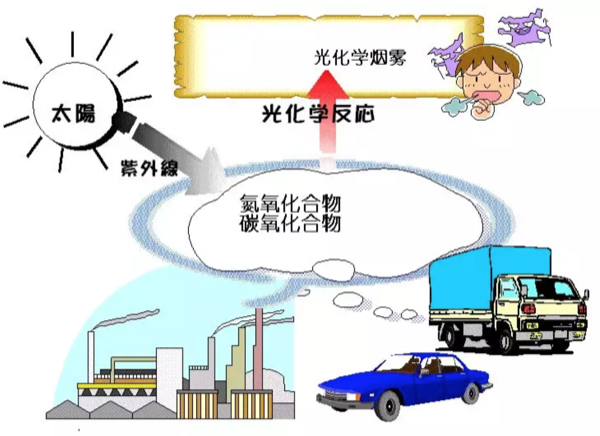
\includegraphics[width=8.33in]{images/voc6}

\hypertarget{vocsux7684ux51cfux6392ux4e4bux8def}{%
\subsection{VOCs的减排之路}\label{vocsux7684ux51cfux6392ux4e4bux8def}}

\hypertarget{ux56fdux5bb6ux5c42ux9762}{%
\subsubsection{国家层面}\label{ux56fdux5bb6ux5c42ux9762}}

我国尚未出现过VOCs污染事件,因此对其关注较晚,2000年,《中华人民共和国大气污染防治法》中仅有诸如有机烃类尾气、恶臭气体、有毒有害气体、油烟等类似概念。

随着灰霾问题的深入研究和环境空气中臭氧浓度升高问题,VOCs逐渐被重视。为改善大气环境质量,促进VOCs削减,我国出台了一系列的政策。2013年,国务院出台《大气污染防治行动计划》,明确要对石化、有机化工、表面涂装、包装印刷等行业实施VOCs综合整治,全国范围内的VOCs减排正式启动。同年,环境保护部编制了《挥发性有机物(VOCs)污染防治技术政策》,为VOCs减排提供了技术规范支持。2015年8月29日第十二届全国人大常委会第十六次会议通过了《中华人民共和国大气污染防治法》,自2000年修订以来,首次增加对VOCs控制要求,从此VOCs减排有了法律依据。这些政策的颁布,从计划到技术、再到立法,逐渐指明我国VOCs减排方向。

在部门规章方面,国家发改委、环保部、财政部、工信部、质检总局、能源局等部委相继出台了有针对性的VOCs污染防治相关文件。各部门相互配合,共同打好VOCs减排攻坚战。

在技术标准方面,我国《大气污染物综合排放标准》(GB162972-1996)对14类VOCs规定了最高允许排放浓度、最高允许排放速率和无组织排放限值,其中包括甲醛、苯、甲苯、二甲苯等挥发性有机物。针对不同的有机污染物排放源以及污染源和环境空气中VOCs的监测技术,截止到2017年,环保部总共制订了15个涉及VOCs的排放标准和20个监测技术方法。从标准实施年限来看,2010年以前,只有3个排放标准和8个监测技术方法,其他都是近几年开始实施。技术标准的制定,为VOCs减排提供了监测和排放依据。

\hypertarget{ux5730ux65b9ux5c42ux9762}{%
\subsubsection{地方层面}\label{ux5730ux65b9ux5c42ux9762}}

为积极推动VOCs减排,各地结合地方实际,出台了一系列相关的政策法规和标准方法。表 1列举了北京和江苏省的VOCs污染防治政策。由表 1可见,我国地方从2010年前后,开始加强对VOCs进行管控。近一两年,VOCs污染防治成为各地大气防治的重点工作,各地不断完善VOCs减排政策措施。

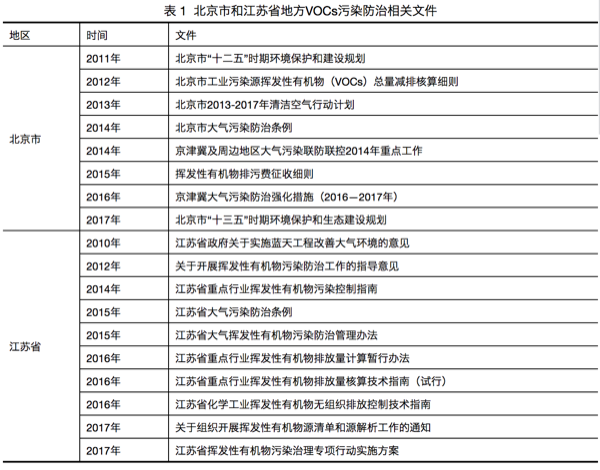
\includegraphics[width=8.33in]{images/voc7}

在技术标准方面,国内出台VOCs排放标准的省市并不多,以北京、江苏、浙江和广东为例,各地根据当地的产业特点,制定了相关VOCs排放标准。近两三年,北京连续制定了12项地方排放标准,涉及的行业有印刷、家具制造、炼油和石油化工、汽车、工业涂装和建筑涂料等;江苏重点针对化学工业和表面涂装行业,制定了相关地方排放标准;浙江以化学合成制药、制鞋、化学涂装、纺织染整行业为重点行业;广东以集装箱制造和电子行业为重点行业。

\hypertarget{vocsux51cfux6392ux6280ux672fux548cux6311ux6218}{%
\subsection{VOCs减排技术和挑战}\label{vocsux51cfux6392ux6280ux672fux548cux6311ux6218}}

对VOCs减排的主要技术思路是源头控制和末端治理。简单的说,源头控制就是从原料开始,减少VOCs的产生。末端治理,顾名思义,将产生的VOCs进行最终的销毁。有两类基本技术,一类是回收技术,对排放的VOCs进行提纯处理,再资源化循环利用。主要包括吸收、吸附、冷凝和膜分离方法等技术。另一类是销毁技术,将排放的VOCs分解化合转化为其他无毒无害的物质。主要包括活性炭吸附、低温等离子、热力燃烧、催化燃烧等技术。

涉及VOCs排放的行业众多,污染物种类繁多,废气成分复杂,因此,在对VOCs减排时,要考虑技术上有效、经济上可行,往往这两者很难平衡,这也是VOCs减排面临的最大的挑战。

\hypertarget{ux5c0fux7ed3-1}{%
\subsection{小结}\label{ux5c0fux7ed3-1}}

因此,虽然我国对VOCs的管控起步较晚,为改善环境空气质量,近年来,我国已将VOCs减排作为一项重点工作,出台了相应的法律、法规、政策、技术规范等,并迅速形成一套体系,为VOCs污染防控指明了方向,提供了支撑和保障。

``大家非常关心中国会不会发生光化学烟雾事件,中国政府也高度关注。我们组织过专家分析,世界历史上发达国家发生的光化学烟雾一般臭氧浓度都达到了600以上,个别城市2000以上。中国的臭氧浓度远低于此,所以中国现在和将来不会、也极少可能会发生光化学烟雾事件。''引用环保部大气环境管理司司长刘炳江的一段话,作为总结,相信我国VOCs减排之路,对环境改善有重要的意义。

作者:远方老友
校稿:广播站王站长、柴胡半夏苏
编辑:栟

\hypertarget{ux751fux6001ux4e94ux884cux4ebaux4f26}{%
\section{生态•五行•人伦}\label{ux751fux6001ux4e94ux884cux4ebaux4f26}}


\includegraphics[width=8.33in]{images/swr1}

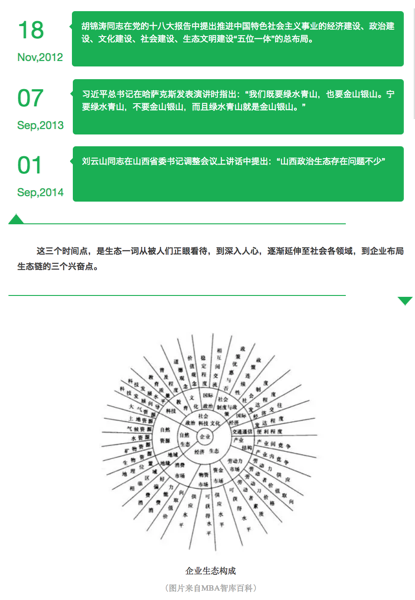
\includegraphics[width=5.76in]{images/swr2}

往事有时令人不忍直视。想当初,环境保护也曾贵为与计划生育相互比肩的两项基本国策之一。然而,一直以来,世人只知后者威加海内,却与前者对面不识。三十年河东,三十年河西。现如今,环境保护俨然已成尚方宝剑,坐拥一票否决权,何止扬眉吐气,大快人心。人们对生态环境保护的关注前所未有。本文也顺着风向,用陈词旧调来赶一次时髦。

一般来说,人们生活的环境通常分为自然环境和社会环境。自然是天与地,天与地之间的万物按照``道''的规律循环不息的现象和状态,包括人类和其他生命世界、物质世界的一切活动。生态是指生物在一定的自然环境下生存和发展的状态。我们人类研究生态,也就是要研究怎样保护和利用自然环境以服务人类的发展,也就是要弄清楚自然是怎样在影响着人类的活动。

研究生态的原理和方法很多,无论东方和西方,还是古代和当代,都有自成体系的表达。本文主要介绍一下在中国古代的五行理论中环境是怎样影响人的。

150年前,马克思提出:``运动着的物质世界是普遍联系和永恒发展的'';3000年前,五行系统理论把这些运动、联系和发展以取象的方法做出了精致的总结。

在五行理论中,根据运动和显现的方式将事物分为木火土金水五类。五行包括气(炁)和象,属于同类五行的事物相互感应。所谓的``天人合一''、``天人相感'',在这个角度讲就是天、地、人、万物之间是一体的,是一直在相互感应的。

为了问题聚焦,我们在这里不具体讨论感应的媒介是电波、磁场,还是量子纠缠,只强调说当某一类五行出现问题的时候,属于这一类五行的所有事物都会受影响。也就是说天地间某一类五行的气(炁)出现问题了,那么赖以这一类五行的气(炁)所支撑的象必然也就要出现问题。我们也不在这里科普具体的五行系统理论,只是应用五行的理论来探讨生态与人伦的问题。这里的人伦包括人的社会伦理和家庭伦理。

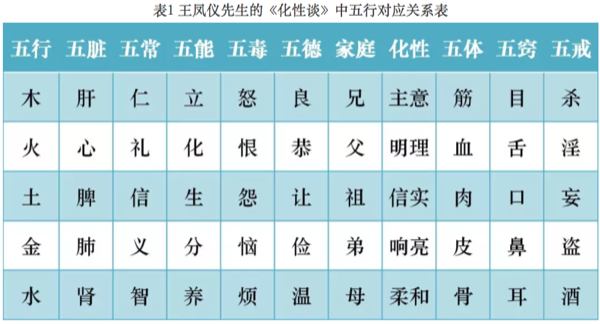
\includegraphics[width=8.33in]{images/swr3}

限于篇幅,此次只简单讲一个离我们最亲近的五行:大地母亲------土五行。

当前,土壤中重金属超标、农田里化肥农药高残留等问题,导致土地受到了普遍破坏。因为破坏的规模和程度足够大,引起了``土''五行气(炁)和象的破坏。

土对应信。所以,当前社会诚信普遍缺失。具体表现为:人们说过的话容易变卦,谈好的事兑现不了(谈十个事情甚至成不了一个),签过的协议无法履行,约定的日期时间不能遵守,制售贩假货泛滥。这里的真实情况不一定是人们主动的不讲诚信,有很大部分是环境在对事件本身产生影响。

土对应怨、脾胃、祖辈、口、安全感。土德受损,人们遇到问题容易怨天尤人,脾胃功能不好,与祖辈少有连接和沟通(包括祭祖),容易打妄语(恶口、两舌、绮语、诳语),贪吃、什么都吃而且吃不到什么好东西。人们普遍缺乏安全感。

土地肥沃、平坦、无污染的地区,人们则是讲信用、不怨人(心胸开阔)、与祖辈亲近(老人容易有儿孙绕膝的天伦之乐)、饮食有节制、不妄语、脾胃好,有安全感。

当土地出了问题,其生长出来的食物自然就要受影响,导致人吃了之后也就有问题。土地贫瘠,土壤中某些元素过剩、毒素残留,会导致食物营养成分不全或者有毒素,人吃了之后自然就会在心理和行为上有相应的表现。吃水培(无土栽培)食物也是如此。长期如此,整个社会也就出现变化。

土地缺失或者供应不足,土地状态被破坏,都会对当地的人和社会状态产生相应影响。

另一方面,一方水土养一方人。医院里的营养师都知道,北方人需要补充维生素的话要吃苹果,而吃香蕉的效果就不如苹果理想。但陕西的苹果的营养对陕西人最适用,本地人最适应本地的农作物。转基因的农作物结出的果实因为无法再当作种子进行发芽生根,所以人吃了会影响生育。

脾属土,主肌肉。人是父精母血交媾而成,从父亲那得了骨,从母亲那得了肉。断奶之后,我们靠土地长出的食物来长肌肉。断奶前应该食母乳。现在人们都是给孩子喂牛奶。而牛奶适合牛的胃,适合牛的营养需求。当前婴儿普遍吃母乳不足,容易导致肌肉和脾胃系统出现问题,长大与母亲不太亲近,也会影响孩子土五行的运转和土德的圆满。

土五行就是这样影响着人与自我的和谐、与家庭的和谐、与社会的和谐。有一个好的生态系统,首先是有好的土地,因为土地不仅是五行之一,还担当着万物的生化、收纳和承载。


\includegraphics[width=8.33in]{images/swr4}

作者:含章
编辑:栟

\hypertarget{ux6cb9ux7530ux73afux4fddux4e4bux75dbux542bux6cb9ux6c61ux6ce5}{%
\section{油田环保之痛------含油污泥}\label{ux6cb9ux7530ux73afux4fddux4e4bux75dbux542bux6cb9ux6c61ux6ce5}}

\hypertarget{ux5e8fux6cb9ux7530ux73afux4fddux7684ux75dbux5904}{%
\subsection{序:油田环保的痛处}\label{ux5e8fux6cb9ux7530ux73afux4fddux7684ux75dbux5904}}

石油作为一种重要的资源,在国民经济发展中具有支柱性地位,不仅支持着工业农业生产,也与每个人的生活息息相关。2011年至2015年间,我国每年的石油开采量持续高于2亿吨。

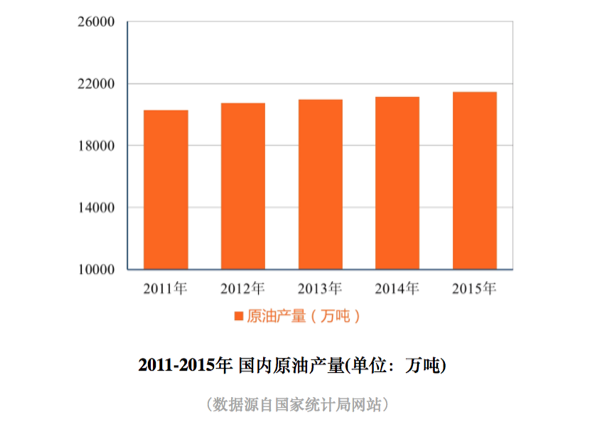
\includegraphics[width=8.33in]{images/youni1}

石油资源开发与使用过程中造成的污染是令全世界头痛的一大难题。举世震惊的墨西哥湾漏油事件,造成了严重的生态灾难,令难以计数的生物遭遇灭顶之灾,沿岸生态遭遇了极大破坏,也使得石油生产过程中的环保问题引起了大众的关注。事实上,在石油业的生产过程中,除了事故导致原油泄露造成的直接环境污染外,在石油开采和加工过程中产生的含油污泥也是一个重要的污染源,且会对周边生态环境造成持续性的危害。

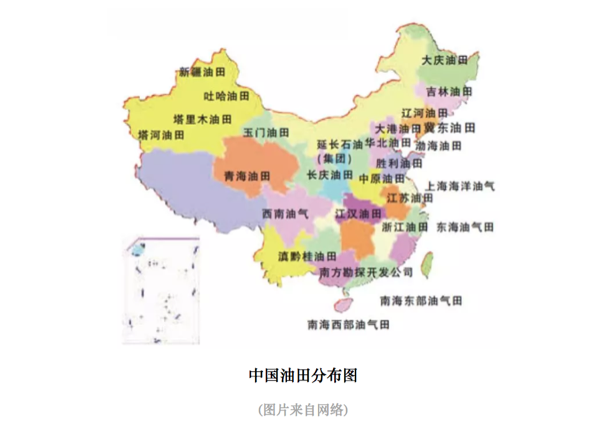
\includegraphics[width=8.33in]{images/youni2}

\hypertarget{ux542bux6cb9ux6c61ux6ce5ux7684ux6765ux6e90}{%
\subsection{含油污泥的来源}\label{ux542bux6cb9ux6c61ux6ce5ux7684ux6765ux6e90}}

含油污泥,简称油泥,是在石油开采、运输、炼制及含油污水处理过程中产生的含油固体废物,是由石油烃类、胶质、沥青质、泥砂、无机絮体、有机絮体以及水和其它有机物、无机物牢固粘结在一起的乳化体系。

含油污泥主要产生在油田和炼油厂,分为3 种类型,即落地油泥、集输油泥和炼厂油泥。落地油泥是在油田开发特别是油井采油生产和井下作业施工过程中,部分原油放喷或被油管、抽油杆、泵及其他井下工具携带至地面,进而渗入地面土壤形成的油泥;集输油泥是储油罐在自然沉降中产生一些油泥,也称之为称为罐底泥;炼厂油泥主要细分有三种,分别为隔油池底泥、溶气浮选浮渣和剩余活性污泥等,其中以浮选浮渣量为最大,占三泥总量的80\%。

\includegraphics[width=8.33in]{images/youni3}

目前,我国每年产生近百万吨的含油污泥,若加上石油化工产生的``三泥''(生化污泥、池底污泥及浮渣),油泥的总量还要大得多,而且炼厂的规模越大,含油污泥的排放量越大。

\hypertarget{ux542bux6cb9ux6c61ux6ce5ux7684ux6210ux5206ux4e0eux7279ux6027}{%
\subsection{含油污泥的成分与特性}\label{ux542bux6cb9ux6c61ux6ce5ux7684ux6210ux5206ux4e0eux7279ux6027}}

含油污泥成分非常复杂,含有大量的老化原油,固体悬浮物,以及细菌质等固体废物,其中原油是主要的成分。油泥中含有数百种有毒有害化合物,其中的某些化合物(多环芳烃等)具有``三致''效应;另外含油污泥中往往含有苯系物、酚类等物质。美国环保署(EPA)将其列为优先污染物,并且对其排放有严格的限制,我国也将油泥列入《国家危险废物名录》。

含油污泥的特性:一般含油污泥的含油率约10\%-50\%,含水率约40\%-90\%。黏度高,难以沉降,脱水效果差,污泥固相颗粒细小,油、水密度差小,这些都是含油污泥黏度大、难以除油脱水的主要原因。

\hypertarget{ux542bux6cb9ux6c61ux6ce5ux7684ux5371ux5bb3}{%
\subsection{含油污泥的危害}\label{ux542bux6cb9ux6c61ux6ce5ux7684ux5371ux5bb3}}

含油污泥因其体积庞大,并含有大量的有毒物质,直接进行排放会占用大面积的土地,同时伴有非常难闻的气味,对附近的土壤、植物、水体、空气造成严重的污染,最终对人体产生极大的危害。

\begin{itemize}
\tightlist
\item
  影响土壤的性质
\end{itemize}

当含油污泥中的石油烃类等物质渗入土壤后,会在土壤颗粒表面黏着,直接影响土壤的通透性,从而造成土壤导水通路的阻塞,进而造成土壤渗水量的下降,透水性的降低,最终使土壤的性质发生改变,直接威胁到土壤中的微生物生存。

\includegraphics[width=8in]{images/youni4}

\begin{itemize}
\tightlist
\item
  危害植物生长发育
\end{itemize}

植物的组织内部能够被含油污泥中的低分子烃类物质渗透,从而破坏植物的正常生理机制;而含油污泥中的高分子烃类会很容易在植株表面形成一层粘性膜,将直接阻塞植株的气孔,植株的水吸收作用以及呼吸和光合作用都会受到严重的影响,最终会造成植物根系的腐烂,植被的破坏将会引起生态系统中食物链的破裂,会导致生态系统中最初级生产者失去制造有机物和氧气的能力。

\includegraphics[width=8.33in]{images/youni5}

\begin{itemize}
\tightlist
\item
  污染水体
\end{itemize}

含油污泥中的石油类污染物浸入地下水后,直接对饮用水资源和地下水资源造成影响,危及人类生命安全。另外,含油污泥处置不当,可能会使石油类污染物在水体中聚集,如码头、港口、河道沿岸等,破坏水体环境。

\includegraphics[width=8.33in]{images/youni6}

\begin{itemize}
\tightlist
\item
  危害空气质量
\end{itemize}

含油污泥中的低沸点有机污染物极易挥发至空气中,有机硫化物、苯类、酚类等有害物质具有致癌、致畸、致突变的作用,随着呼吸进入人体,直接对人体的肺、胃、呼吸系统、神经中枢系统产生严重的危害。

\includegraphics[width=8.33in]{images/youni7}

\hypertarget{ux76f8ux5173ux63a7ux5236ux6807ux51c6}{%
\subsection{相关控制标准}\label{ux76f8ux5173ux63a7ux5236ux6807ux51c6}}

在国家层面,目前与含油污泥相关的控制标准有《危险废物填埋污染控制标准》(GB18598---2001)、《危险废物焚烧污染控制标准》(GB18484---2001)、《农用污泥中污染物控制标准》(GB4284---84)。在《危险废物填埋污染控制标准》和《危险废物焚烧污染控制标准》标准中,将含油污泥归类为危险固体废物,但并没有对含油污泥的油含量提出量化指标。在《农用污泥中污染物控制标准》中,对污泥中的矿物油含量做了明确规定,要求土壤中矿物油最高允许含量不得超过3000 mg/kg(≤0.3%)。地方层面主要有以下三省份制定了相关标准:2010年12月,黑龙江省发布了《油田含油污泥综合利用污染控制标准》,明确规定了含油污泥用于农用、铺设油田井场和通井路的污染物控制标准;2016年7月,陕西发布《含油污泥处置利用控制限值》,规范含油污泥回收利用处置;2017年6月,新疆维吾尔自治区发布《油气田含油污泥综合利用污染控制要求》。

\includegraphics[width=8.33in]{images/youni8}

\hypertarget{ux542bux6cb9ux6c61ux6ce5ux7684ux5904ux7406ux5904ux7f6e}{%
\subsection{含油污泥的处理处置}\label{ux542bux6cb9ux6c61ux6ce5ux7684ux5904ux7406ux5904ux7f6e}}

如果含油污泥得不到妥善处理,将造成资源的巨大浪费,同时也会对环境造成不可挽救的破坏。因此,采用合适的处理方法对含油污泥进行资源化与无害化处理,不仅可以减少环境污染,而且还能达到资源再利用的目的。当前的油泥处理技术主要包括热解法、调质离心分离、固化处理、焚烧、焦化、填埋、溶剂萃取、热碱水洗、电化学技术、生物处理 (包括地耕法、堆肥法、污泥微生物反应器法)等。

由于含油污泥来源广泛、成分复杂,同时处理技术种类繁多,且都存在各自的应用弊端和适用范围(不同技术的特点比较如下表),目前尚无任何一种技术可以作为处理所有类型含油污泥的理想方法。通常要根据油泥的来源及特性,有针对性地选择一种或者多种组合技术实现油泥的治理。

\includegraphics[width=8.33in]{images/youni9}

\hypertarget{ux5904ux7406ux5b58ux5728ux7684ux96beux70b9ux548cux6280ux672fux5c55ux671b}{%
\subsection{处理存在的难点和技术展望}\label{ux5904ux7406ux5b58ux5728ux7684ux96beux70b9ux548cux6280ux672fux5c55ux671b}}

随着新环保法的通过,各地对油田环保的要求越来越高,含油污泥的随意排放将不再可能,各地隐藏的污染也被逐渐揭开。这对污泥处理行业来说,无疑发展前景利好。尽管油泥处置发展前景好,市场也很大,但是目前含油污泥处置也存在一些难点,同时对其发展前景进行梳理如下:

\begin{itemize}
\item
  含油污泥中最难处理的是重质油油泥,其黏度大,沥青质及胶质含量高,回收难,在现有的工艺设备处理过程中成本较高,设备折旧快,因此降黏预处理是此类油泥处置的重要环节;
\item
  热解方法由于是在厌氧环境条件下热源对含油污泥间接加热,能够通过油气组分的挥发分离实现油泥中石油组分的回收,同时降低残渣中的含油率,是一种油泥无害化与资源化的综合处理工艺。因此,该技术是近三年来油泥处置行业极为推崇的热点实用工艺,尤其在能源价格低、油泥组分中砂质组分含量的西北地区的油泥,更适合推广该技术;
\item
  热解方法尽管处理含油污泥非常实用有效,但是与调质离心等减量化工艺相比,仍存在耗能高、处理规模小等问题,因此,在以后的研究过程中亟待开发提高热解处理效果与规模的带有新型热源的新一代热解设备;
\item
  微生物及植物修复方法尽管修复周期长,却非常适合低浓度石油污染的场地及油泥处理,是物理与化学方法后续深度处理含油污泥的重要补充措施。为了使植物修复最终成为解决实际环境问题的有效手段,如何将石油污染的植物修复从盆栽实验的研究成功转向田间试验及实际的工程尚需进一步的深入研究;
\item
  目前含油污泥高级氧化技术在东北及西北地区油田的油泥处理工程中得到有效的实际应用,但该方法存在药剂成本高、处理的油泥残留化学药剂等问题,因此开发环境友好、氧化能力突出的绿色修复药剂就显得尤为重要;
\item
  目前油泥处理的验收标准往往是以含油率为重要指标,但是缺乏具体的石油烃组分的定性定量分析,鉴于不同组分的生物有效性及环境风险有很大差异,因此在以后的研究中有必要深度细化处理后含油污泥的石油组分含量,进一步明确验收标准。
\end{itemize}

作者:OILs
校稿:周宁、爱杯子的王小咖
编辑:栟

\hypertarget{ux65afux5fb7ux54e5ux5c14ux6469ux516cux7ea6ux548cux5b83ux9501ux4f4fux7684pops}{%
\section{斯德哥尔摩公约和它``锁''住的POPs}\label{ux65afux5fb7ux54e5ux5c14ux6469ux516cux7ea6ux548cux5b83ux9501ux4f4fux7684pops}}

\hypertarget{ux7ba1ux63a7ux6301ux4e45ux6027ux6709ux673aux6c61ux67d3ux7269ux7684ux65afux5fb7ux54e5ux5c14ux6469ux516cux7ea6}{%
\subsection{管控持久性有机污染物的斯德哥尔摩公约}\label{ux7ba1ux63a7ux6301ux4e45ux6027ux6709ux673aux6c61ux67d3ux7269ux7684ux65afux5fb7ux54e5ux5c14ux6469ux516cux7ea6}}

随着国家层面对环保的重视,公众也越来越多的开始关注环境污染问题。大家可能时常听到一个词------POPs,一个读起来略带喜感的单词缩写,但它指代的物质却十分``恐怖''。POPs是持久性有机污染物(Persistent Organic Pollutants)的简称,是指那些具有生物蓄积性、能够通过各种环境介质长距离迁移并长期存在于环境中,对人类健康和生态环境造成严重危害的天然或人工合成的有机化合物,其污染的复杂性远超过常规污染物。一些POPs具有三致效应(致畸、致癌、致突变),它们的危害往往具有隐蔽性和突发性的特点,一旦发生重大污染事件,将产生灾难性后果并持续危害几代人。例如1968年3月发生在日本的米糠油事件,由于管理不善,致使生产米糠油时混入多氯联苯,产品被人食用后导致中毒,患病者超过5000人,30余人死亡,实际受害者约13000人。症状主要表现为咳嗽不止,肝功能下降,全身肌肉疼痛,重者发生急性肝坏死、肝昏迷等,及至死亡。副产品之一的黑油作为饲料喂养家禽后造成数十万只家禽死亡。这是一起典型的POPs中毒事件,当时震惊了全世界。

为此,2001年联合国环境规划署通过了旨在控制POPs的《斯德哥尔摩公约》(下文简称公约),作为保护生态环境和人类健康免受有机污染物危害的全球行动。目前,已有包括我国在内的179个国家和地区加入了公约,从缔约国数量上可以看出公约的国际影响力,同时也能看出各个国家对于POPs污染的重视。其中公约规定的12种POPs,即氯丹、艾氏剂、狄氏剂、异狄氏剂和七氯、滴滴涕、六氯苯、多氯联苯、毒杀芬、灭蚁灵、多氯二苯并呋喃、多氯二苯并-对-二恶英等,被称为``肮脏的一打(dirty dozen)'',受到缔约国的严格控制与削减。在国际公约的推动下,国际上有关POPs的相关研究也逐步深入,已成为环境科学研究中最受关注的热点领域之一(见图1)。

\includegraphics[width=8.33in]{images/gongyue1}

随着人类经济活动的快速发展,许多新型POPs,如氯化石蜡、全氟化合物、溴代阻燃剂等也不断在各种环境介质中被发现,逐渐成为关注的焦点。这些物质绝大多数是正在大量生产和使用的化工产品,目前尚未对其生产排放进行有效管控,而且相关的人体健康风险、生态风险和毒理学数据还较为缺乏,难以准确评估其生态和健康效应。

\includegraphics[width=8.33in]{images/gongyue2}

公约如何将某种POPs列入管控对象呢?公约规定了任一缔约国均可向秘书处提交旨在将某一化学品(拟增列POPs)列入公约附件的提案。而公约秘书处将提案转交给持久性有机污染物审查委员会(POPRC)后,将依次审查其是否符合公约附件D(化学品的持久性、生物富集性、长距离迁移能力及不利影响),附件E(评价该化学品是否会因其远距离迁移而对人体健康和/或环境产生重大不利影响)和附件F(涉及社会经济考虑因素的信息)对POPs的要求,如果全部符合,POPRC会根据风险管理评价的结果提议是否由缔约国大会审议该化学品以便将其列入附件并规定相应的管控措施(流程见图3)。

2009年5月,在瑞士日内瓦举行的缔约方大会第四届会议决定将全氟辛烷磺酸及其盐类、全氟辛基磺酰氟、四溴联苯醚、五溴联苯醚、六溴联苯醚、七溴联苯醚、十氯酮、六溴联苯、林丹、五氯苯、α-六六六、β-六六六等新增化学物质列入公约附件的受控范围。2011至2015年间的缔约方第五次会议、第六次会议以及第七次会议又分别决定将硫丹及硫丹硫酸盐、六溴环十二烷、多氯萘、六氯丁二烯和五氯苯酚等物质增列到公约POPs名单。2017年5月第八次会议将十溴联苯醚、短链氯化石蜡以及六氯丁二烯正式增列为公约POPs候选名单。目前正在进行审查的物质包括三氯杀螨醇、全氟辛酸及其相关物质。

\includegraphics[width=8.33in]{images/gongyue3}

\hypertarget{popsux7684ux6301ux4e45ux6027}{%
\subsection{POPs的持久性}\label{popsux7684ux6301ux4e45ux6027}}

``环境持久性''是POPs最主要的特点之一,是界定一种物质是否为POPs以及筛选新型POPs的重要判据,也是评价有机污染物对环境和人类潜在危害的基础以及开展化学品风险评估的关键依据。公约附录D关于持久性的评价标准为:对于通过空气大量迁移的化学品,其在空气中的半衰期应大于两天、或者该化学品在水中的半衰期大于两个月、或在土壤/沉积物中的半衰期大于六个月;或该化学品具有其他足够持久性、因而足以有理由考虑将之列入本公约适用范围的证据。

\includegraphics[width=8.33in]{images/gongyue4}

\hypertarget{popsux7684ux751fux7269ux5bccux96c6ux6027ux653eux5927ux6027}{%
\subsection{POPs的生物富集性/放大性}\label{popsux7684ux751fux7269ux5bccux96c6ux6027ux653eux5927ux6027}}

生物富集和放大性是指化学物质可被生物组织吸收,并在生物体内持续累积,而且这些物质的浓度会沿着食物链/网传递(图5),随着营养级升高呈现放大趋势,在高等生物体内出现高浓度,影响高等生物的健康。公约对POPs的生物富集性/放大性的规定为:(1)表明该化学品在水生物种中的生物浓缩系数或生物富集系数大于5000,或如无生物浓缩系数和生物富集系数的数据,但有logKow大于5的证据;(2)表明该化学品有令人关注的其他原因的证据,例如在其他生物中的生物富集系数较高,或具有高度的毒性或生态毒性;(3)生物监测数据显示,该化学品所具有的生物富集潜力足以有理由考虑将其列入本公约的适用范围。

\includegraphics[width=8.33in]{images/gongyue5}

\hypertarget{popsux7684ux957fux8dddux79bbux8fc1ux79fbux80fdux529b}{%
\subsection{POPs的长距离迁移能力}\label{popsux7684ux957fux8dddux79bbux8fc1ux79fbux80fdux529b}}

POPs具有长距离迁移特性,以大气和水体为载体,通过``高山冷捕集效应''和``全球蒸馏效应''到达高海拔的偏远高山地区和高纬度的极地地区,从而导致全球范围的污染。公约对远距离环境迁移的评判标准如下:

(1)在远离其排放源的地点测得的该化学品的浓度可能会引起关注;

\begin{enumerate}
\def\labelenumi{(\arabic{enumi})}
\setcounter{enumi}{1}
\tightlist
\item
  监测数据显示,该化学品具有向环境受体转移的潜力,且可能已通过空气、水或迁徙物种进行了远距离环境迁移;
\end{enumerate}

(3)环境转归特性和/或模型结果显示,该化学品具有通过空气、水或迁徙物种进行远距离环境迁移的潜力,以及转移到远离物质排放源地点的某一环境受体的潜力。

\includegraphics[width=8.33in]{images/gongyue6}

\hypertarget{ux4e2dux56fdux7684ux5b9eux65bdux8ba1ux5212}{%
\subsection{中国的实施计划}\label{ux4e2dux56fdux7684ux5b9eux65bdux8ba1ux5212}}

我国政府于2001年5月23日签署了《关于持久性有机污染物的斯德哥尔摩公约》,2004年6月25日第十届全国人大常委会第十次会议做出了批准《斯德哥尔摩公约》的决定。公约于2004年11月11日对中国正式生效。依据公约第7条要求,中国政府编制并向缔约方大会递交了履行公约的《国家实施计划》。

我国作为经济快速发展的国家,面临着极为复杂和严峻的环境问题。鉴于新型POPs的巨大累积产量,我国新型POPs引起的环境污染和健康风险问题比其它国家更为严重。目前,通过科研人才培养、建立相应的专业实验室以及设立相关的科研项目,已经大大提高了对于POPs特别是新型POPs的检测水平和防控能力。然而,作为化学品生产和使用大国,我们仍面临巨大挑战,对于新型POPs在环境行为、生态毒理、环境风险以及化学品管理等方面依旧缺乏研究基础和成熟经验,在履行《斯德哥尔摩公约》和保护生态环境上依然任重道远。

斯德哥尔摩公约的网址:

\url{http://www.pops.int/}

\url{http://www.un.org/chinese/documents/decl-con/popsp/index.htm}

参考文献:

\href{陈心想,耿增超。西北农林科技大学学报(自然科学版),2013,41:\%20167-174.}{1} COP. Listing of short-chain chlorinated paraffins in Annex A to the Convention (UNEP/POPS/COP.8/11). 2017.

\href{Kezhen\%20Qian,\%20Ajay\%20Kumar,\%20et.al.\%20Renew.\%20and\%20Sustain.\%20Energy\%20Reviews,\%202015,\%2042:\%201055-1064.}{2} Feng Y, Tian J, Xie H Q, et al.~Effects of Acute Low-Dose Exposure to the Chlorinated Flame Retardant Dechlorane 602 and Th1 and Th2 Immune Responses in Adult Male Mice. Environ. Health. Persp, 2016. 124. 1406-1413.

\href{Puga\%20A\%20P,\%20Abreu\%20C\%20A,\%20et\%20al.\%20J.\%20of\%20Environ.\%20Manage.,\%202015,\%20159:\%2086–93.}{3} Giesy J P, Kannan K. Global distribution of perfluorooctane sulfonate in wildlife. Environ. Sci. Technol. 2001. 35. 1339-1342.

\href{Khan\%20S,\%20Cai\%20Chao,\%20et\%20al.\%20Environ.\%20Sci.\%20\&\%20Technol.,\%202013,\%2047\%20:\%208624-8632.}{4} Liu L Y, He K, Hites R A, Salamova A. Hair and Nails as Noninvasive Biomarkers of Human Exposure to Brominated and Organophosphate Flame Retardants. Environ. Sci. Technol. 2016. 50. 3065-3073.

\href{Bi\%20H,\%20Huang\%20X,\%20et\%20al.\%20Small\%202014,\%2010,\%203544.}{5} Pedersen K E, Letcher R J, Sonne C, Dietz R, Styrishave B. Per- and polyfluoroalkyl substances (PFASs) - New endocrine disruptors in polar bears (Ursus maritimus)? Environ Int. 2016. 96. 180-189.

\href{Gupta\%20V\%20K,\%20Ganjali\%20M\%20R,\%20et\%20al.\%20Chemical\%20Engineering\%20Journal,\%202012,\%20197:\%20330.}{6} Vives I, Grimalt J O, Lacorte S, Guillamón M, Barceló D. 2004. Polybromodiphenyl ether flame retardants in fish from lakes in European high mountains and Greenland. Environ. Sci. Technol. 2004. 38. 2338-2344.

\href{Liu\%20R\%20L,\%20Liu\%20Y,\%20et\%20al.\%20Bioresourse\%20Technology\%202014,\%20154:\%20138.}{7} 王亚韡, 蔡亚岐, 江桂斌. 斯德哥尔摩公约新增持久性有机污染物的一些研究进展. 中国科学. 2010. 40. 99-123.

\href{Gao\%20F,Qu\%20J\%20Y,\%20et\%20al.\%20Electrochim.\%20Acta\%202016,\%20190:\%201134.}{8} 张焘, 仇雁翎, 朱志良, 赵建夫. 有机污染物的持久性评价方法研究进展. 化学通报. 2012. 75. 420-424.

作者简介:田浩廷,山东人,博士毕业于南京大学环境学院,2016年入职临沂大学,青椒一枚,目前于中科院生态环境研究中心从事在职博士后研究,研究方向为持久性有毒有机污染物的环境界面过程、污染物界面催化降解。

校稿:yufree,大石

编辑:丫头晚安

\hypertarget{ux65e5ux5e38ux751fux6d3bux4e2dux7684ux5316ux5b66ux54c1ux65b0ux578bux6709ux673aux6c61ux67d3ux7269ux7b80ux4ecb}{%
\section{日常生活中的化学品------新型有机污染物简介}\label{ux65e5ux5e38ux751fux6d3bux4e2dux7684ux5316ux5b66ux54c1ux65b0ux578bux6709ux673aux6c61ux67d3ux7269ux7b80ux4ecb}}

\hypertarget{ux524dux8a00-2}{%
\subsection{前言}\label{ux524dux8a00-2}}

通常来说,人们对于能直接感官感受到的环境污染的危害认识较为清楚,比如灰暗的天空、黑臭的河水、以及遍地的塑料垃圾。但是你有没有想过,其实在一些表面看来极其干净的环境中也会存在高浓度的有毒有害污染物,而这些污染物对人体健康的损害可能并不比直接可感官感觉到的环境污染小。以北美五大湖为例,它风景优美,湖水清澈。可就是这样美丽的外表下却有着一颗``肮脏的心''。表面上,五大湖的湖水比国内多数湖泊、河流看上去要干净,但其中的某些持久性有机污染物 (persistent organic pollutants, POPs) 的浓度远高于国内湖泊。这也是外国人不吃淡水鱼的原因之一,因为淡水鱼体内的POPs浓度确实高于海水鱼。

POPs是指能持久存在于环境中,具有长距离迁移能力,通过食物链(网)累计,并且对生物和人体具有毒性效应的一类有机化学品。目前POPs的生产和使用已经受到《斯德哥尔摩公约》的严格限制,但在可以预见的将来,所有被列入《斯德哥尔摩公约》的POPs均会退出化学品市场。随着POPs的退出,其他新型有机污染物的研究成为目前环境化学领域的研究热点。这些新型有机污染物常常以化学品,也即是人工合成添加剂的形式出现,影响人体健康。化学品对人体造成损害有两个必要条件,其一是化学品具有毒性效应,其二是人体和化学品有接触途径。在我们日常生活中能够接触到的化学品品种众多,包括紫外线吸收剂、抗氧化剂、阻燃剂、塑化剂、光引发剂等,本文将重点介绍合成酚类抗氧化剂、双酚类物质、光固化材料等三类。这些化学品是一类富含争议的物质,它们在保障人们现代生活品质的同时,也给我们造成了一定的困扰。

\includegraphics[width=8.33in]{images/epc1}

\hypertarget{ux5b9eux4f8b}{%
\subsection{实例}\label{ux5b9eux4f8b}}

1 合成酚类抗氧化剂,天使还是魔鬼?

为阻止或延缓橡胶、塑料、纤维等人工合成有机高分子材料在使用过程中的氧化降解,抗氧化剂被广泛应用。由于天然抗氧化剂的稳定性较差,目前广泛使用的是人工抗氧化剂。目前我国市场上最常使用的抗氧化剂为BHT。BHT化学名称为2,6-二叔丁基-4-甲基苯酚,它是由对甲酚、异丁醇为原料,以浓硫酸作为催化剂,氧化铝为脱水剂,反应生成的产物。根据世界经济合作与发展组织 (OECD) 的统计BHT的使用主要分布在以下领域:橡胶(27\%),塑料(27\%),矿物油/燃料(17\%),食品/药品/化妆品(12\%),动物饲料/宠物食品(11\%),打印油墨(6\%)。目前,BHT的污染已经非常普遍,且存在于多种环境介质中,例如河水、底泥、污泥、室内灰尘等。

在食品应用方面,最近发表在Nature Communications上的文章揭示了一个有趣的现象,给吃货们找到了一个自我安慰的理由。研究者发现,添加到食物中的BHT会干扰人体消化系统与大脑间的信号传递,从而导致人脑产生更强的饥饿感,想吃更多的食物,进而导致肥胖。好想说``真的不是我馋,是BHT让我很饿''。

没有直接研究表明BHT具有毒性,甚至有研究认为BHT可以清除人体内的氧化自由基,因此具有抗癌的功效。然而,BHT可以在生物体内和环境介质中被转化为多种产物。目前的毒理学研究表明其部分转化产物的毒性显著高于BHT。例如,BHT-Q在浓度为10-6mol/L时即可通过生成H2O2进而破坏人体的DNA,从而表现出较强的基因毒性。更值得注意的是,我们的研究显示BHT可以在污水处理厂(厌氧-缺氧-好氧的活性污泥处理系统)中转化为相应的毒性产物(BHT-CHO,BHT-Q,BHT-quinol)。经过污水处理厂处理的污水,BHT的浓度会显著下降,但相关转化产物的浓度会显著上升,增加了污水处理厂出水回用的潜在危害。

\includegraphics[width=8.33in]{images/epc2}

2 双酚类污染物,无处不在

双酚A (BPA) 是一种人工合成的化学品,作为增塑剂、抗氧剂、热稳定剂等添加剂广泛应用于塑料、纸币、热敏纸等日常生活用品中。此外,BPA也是一种重要的有机化工原料,主要用于生产聚碳酸酯和环氧树酯等聚合材料,BPA在2011年的全球产量超过550万吨。BPA的主要毒性表现为内分泌干扰效应,尤其是对婴幼儿内分泌系统的危害,能导致内分泌失调,威胁胎儿和儿童的健康。为了对塑胶进行分类,美国塑胶工业协会 (Society of the Plastics Industry) 自1988年起,对塑胶进行编码分类,塑胶分类标志的符号包含了顺时针转的箭头,形成一个完整的三角形,并将编码包围于其中,如图7所示。一般来讲,塑胶分类标志为1、2、4、和6的塑料不太可能在生产中与BPA接触,而有一些塑胶分类标志为3或7的塑料在生产中可能会接触到BPA。自2011年6月1日起,我国已禁止进口和销售含有BPA的婴幼儿奶瓶。

\includegraphics[width=8.33in]{images/epc3}

随着对BPA使用风险的关注和日趋严格的法规控制,市场上出现结构和性质与BPA相似的新型替代化合物,统称为双酚类化合物(Bisphenols, BPs), 它们在与人们日常生活密切相关的购物小票、纸币、食品包装材料中广泛使用。在日常生活中接触购物票、纸币等物质时,BPs可透过皮肤吸收进入人体。加拿大学者的研究发现手持购物小票5分钟,即可使这类物质透过皮肤吸收进入人体。因此,相关职业人群如收银员体内BPs的浓度显著高于普通人群。目前,关于BPs这类替代化合物对人体健康的影响尚处于研究当中,暂无足够的数据来判定其对人体健康的影响。基于BPs这类替代化合物与BPA结构的类似性,我们预测部分BPs可能具有与BPA类似的毒性效应。

\includegraphics[width=8.33in]{images/epc4}

3 光固化材料--绿色化学真的绿色吗?

光固化材料是指光引发剂在光照(一般为紫外光)作用下产生活性物质(自由基等),从而引发单体发生的聚合反应所生成的聚合材料。与传统的聚合反应相比,光敏聚合反应具有反应所需能量低、无挥发性有机污染物释放等优点。因此,光固化材料的生产过程被称为绿色化学。目前,光固化材料广泛应用于紫外打印、紫外涂料、以及光敏树脂3D打印等领域。

\includegraphics[width=8.33in]{images/epc5}

2005年,欧洲市场上的雀巢婴幼儿奶粉中发现高浓度的光引发剂污染,首次引起了科学家对光固化材料中光引发剂污染的重视。事后的研究发现奶粉中的光引发剂污染来源于包装材料中的光敏打印油墨。近年来的研究已经在食品包装材料和3D打印产品中检测到20多种光引发剂。由于光固化材料在室内环境中有大量应用,北京市室内灰尘中也检测到了高浓度的光引发剂。这类物质的毒性主要表现为内分泌干扰效应。加州大学的研究发现,使用光敏树脂3D打印器皿培养斑马鱼鱼卵,可以观察到明显的斑马鱼发育毒性。由此可见,``绿色化学''并不绝对的绿色。目前,世界各国并无关于光引发剂使用的限制。欧洲及日本的打印协会建议停止在食品包装材料的打印油墨中使用某些高毒性的光引发剂,但该建议尚未形成法律条文。

\hypertarget{ux7ed3ux8bed-2}{%
\subsection{结语}\label{ux7ed3ux8bed-2}}

传统的水污染及土壤污染等只会对生活于其区域的人群产生影响。即使近年来在我国北方影响范围比较大的雾霾,人们也可以通过迁移到更干净的区域进行规避。与传统的空气、水、土壤等污染不同,只要你选择现代生活,你就无法避免形形色色的合成添加剂。但我们也无需过度担心,因为污染物的毒性总是与剂量相关联。以``前言''中所述北美淡水鱼为例,尽管鱼体内含有较高浓度的污染物,但只要找到合理的摄入标准,就不会对人体健康产生损害。

\includegraphics[width=8.33in]{images/epc6}

同理,对于生活中形形色色的添加剂危害的预防,最重要的还是深化基础科学研究。由政府加大投入,相关领域科学家对添加剂的生物安全性进行评估,促进政府制定相应的法律法规。目前,我国有4.6万种化学品在生产和使用,每年还有几百种新增加的化学品进入市场,要全面评估所有化学品对人体的健康风险工作量巨大。可喜的是,近年来科学家开始重视基于计算机的定量结构-效应关系(QSPR)模型方法,QSPR可帮助我们初步筛选具有潜在危害的目标化学物质,对筛选出来的可能具有危害性的化学物质可进行进一步的实验评估。对毒性较大物质的使用进行限制或禁止,而对毒性较小且产品替代比较困难的物质可在相关标准下进行使用,从而最大限度地提升生活品质,降低化学品(添加剂)的使用风险。

作者:L润Z
校稿:看透,胜利屯屯长
编辑:李立平

\hypertarget{ux4ebaux864eux5171ux5b58ux4e3eux6b65ux7ef4ux8270}{%
\section{人虎共存,举步维艰}\label{ux4ebaux864eux5171ux5b58ux4e3eux6b65ux7ef4ux8270}}

最近,《东北虎豹国家公园总体规划》征求意见稿发布,标志着虎豹公园的范围、定位、功能分区、重点工程、体质机制等一系列重要问题基本敲定,这实属不易。其实,虎豹公园早在三年前就开始筹划建立了,而《总规》的定稿和发布却经历了漫长而复杂的过程。即使如此,对于东北虎豹种群的持久性保护而言,这也仅仅是万里长征的第一步。

\includegraphics[width=5.62in]{images/tiger1}

\hypertarget{ux80ccux666fux4ecbux7ecd}{%
\subsection{背景介绍}\label{ux80ccux666fux4ecbux7ecd}}

虎豹国家公园的缘起归功于北京师范大学的葛建平教授及其团队,经过在吉林珲春的长期观测,该团队最终确定在我国境内长期活动的东北虎共27只,东北豹42只。2015年两会期间,总书记在参加吉林省代表团审议时得知此事并给与重视,随即,东北虎豹重点保护工程开始在国家层面上谋划实施。

\includegraphics[width=5.79in]{images/tiger2}

2015年冬,我跟随规划项目组到东北虎豹在我国的集中分布区------吉林延吉考察,深入了珲春、汪清、天桥岭等地的天然林区,探访了东北虎豹的栖息地。但我们并不走运,几天下来,并未见虎豹踪影。仅看到林中野猪留下的些许蹄印,风折或腐朽掉的红松枝干,河岸边被雾凇装扮的玉树琼花,以及山丘上望不到边际的皑皑白雪。

\includegraphics[width=8.33in]{images/tiger3}

我本想,有这样美妙的自然环境,再加上虎豹带来的旅游效益,当地居民应该衣食无忧,幸福感爆棚。没成想,这看似祥和的环境却并不太平。

与美国、加拿大等国家不同,我国人口数量太大,并且分布广泛,除了沙漠和高山区,真正的无人区很少。在虎豹国家公园内,就分布有90000多人口,这无疑造成了大量的人为干扰。然而,作为``森林之王'',东北虎的活动范围巨大,成年雄虎的家域面积可达600-800km2,成年雌东北虎家域面积也在300-500 km2(马建章和金崑,2003)。即使经过几次扩增,虎豹公园的面积已经扩大至1.49万km2,但对几十只东北虎和东北豹来说,其实并不富裕,更何况同时还居住着这么多的人!于是,人虎矛盾在所难免。

\hypertarget{ux4ebaux864eux77dbux76feux96beux4ee5ux8c03ux548c}{%
\subsection{人虎矛盾,难以调和}\label{ux4ebaux864eux77dbux76feux96beux4ee5ux8c03ux548c}}

一、虎豹对当地居民财产和人身安全的威胁

虎豹均属于大型捕食性动物,捕杀林中野猪、狍子等是它们的日常课业,当然,也包括居民畜养的牛羊!关于虎豹猎杀当地居民家畜的报道已经屡见不鲜。当地人介绍,有农户家的羊在一晚上就被老虎咬死十几只,据说是为了给幼崽传授捕食技术,可见母爱之伟大!

但是,这里有一笔经济账,那就是:谁为老虎的``晚餐''买单,价格几何?目前,对于虎豹造成的家畜死伤,一般由国家野生动物保护部门负责补贴。可以说,虎豹是公款吃喝,好不自在。但是,补贴总归是补贴,对当地农户来说,还是会有相当一部分损失的。

至于人身安全,更是不必多说,与虎豹做邻居,但凡智商正常的人一般都不会感觉十分保险。

二、人类活动对虎豹的直接伤害

在东北林区,几乎家家都会一门简单的手艺,那就是用钢丝来制作猎套。在山林中,用猎套捕杀野生动物十分奏效,当然,也包括东北虎。

\includegraphics[width=8.33in]{images/tiger4}

虽然,以当地林业局为主的野生动物保护部门不断开展山间清套行动。巡山清套行动也写进了《总规》中,但是,要从根本上遏制套猎行为,仅仅依靠清套行动是远远不够的,因为它已经成为林区人民的生活方式和文化。要彻底消除套猎现象,应该要做出多方面的努力,包括自然教育、法制建设甚至要从社会生活理念和方式上发生转变。

三、居民生产生活方式与虎豹保护的相互影响

如今的东北林区,``棒打狍子瓢舀鱼''的生活虽然有些夸张,但采松子、打野味还是稀松平常的。无论是采集还是狩猎,都会造成虎豹生存环境的破坏和自然猎物的减少。此外,公园内的家畜散养和土地开垦同样会对自然生态系统产生重要影响。据统计,虎豹公园内的散养黄牛达到60000多头,大量的黄牛与马鹿、梅花鹿等虎豹猎物竞争了食物和生存空间,同时也是人虎矛盾加剧的潜在风险,因为虎豹并不了解吃下这些黄牛其实是违法的。

《总规》中提出要禁养退牧还草,并清收开垦土地,然而,如何进行合理的禁养退牧和土地清收,并对当地以此为生的农民做出合理补偿,又将十分复杂。

\includegraphics[width=8.33in]{images/tiger5}

\hypertarget{ux8f6cux53d8ux601dux8defux4ebaux9000ux864eux8fdb}{%
\subsection{转变思路,人退虎进}\label{ux8f6cux53d8ux601dux8defux4ebaux9000ux864eux8fdb}}

就东北虎豹的有效保护和种群延续,《总规》提出了一系列的措施,包括虎豹种群保护、栖息地保护修复、扩散廊道疏通等等。然而,在活动范围、取食范围,甚至是整个生态位,人与虎、豹都存在太多的重叠和矛盾,其主导因素,完全在人。因此,若不能实现园区人口的明显下降,将很难实现对虎豹种群的持久性保护。

然而,要90000多人搬离家乡谈何容易!如此看来,在某种程度上,虎豹保护已经超出了物种保护的范畴,并成为了一个社会问题。东北经济正值转型期,虎豹国家公园的命运也将被绑定其中。我们更希望看到的是,国家公园能在区域水平上助力经济转型。在严格保护的同时,深入发掘虎豹的社会文化价值,形成一系列的生态旅游产品和自然教育品牌。比如,依托冰雪文化和虎豹文化,在公园外围打造``特色小镇''、``田园综合体''等等,以产业发展拉动公园内部居民迁出,同时形成经济效益,反哺公园建设。

\includegraphics[width=8.33in]{images/tiger6}

人虎矛盾固然不可调和,但只要人走了,虎豹自然就来了。然而,我们也不能就保护而谈保护,不惜一切代价把人赶走,而是要转变思路,使得国家公园体系建设更好的服务于当地社会经济发展。希望东北虎豹国家公园的建立,真正能像吉林省省委书记巴音朝鲁所说的:``东北虎、豹将成为吉林绿色转型的魂。''

参考文献:马建章,金崑. 2003. 虎研究. 上海: 上海科技教育出版社.

作者简介:张雷,中科院生态环境研究中心博士研究生,生态学专业。

作者:雨田
校稿:广播站王站长
编辑:竹而乐

\hypertarget{ux53efux6301ux7eedux793eux533aux5efaux8bbeux6848ux4f8bux5317ux4eacux5f53ux4ee3momaux516cux5bd3}{%
\section{可持续社区建设案例------北京当代MOMA公寓}\label{ux53efux6301ux7eedux793eux533aux5efaux8bbeux6848ux4f8bux5317ux4eacux5f53ux4ee3momaux516cux5bd3}}

可持续发展是一个比较容易引起人们困扰的概念,从1987年《我们共同的未来》出版以来,可持续发展的概念已经走过了三十年。目前全世界人们最公认的可持续发展的核心思想就是``既能满足当代人的需要,又不对后代人满足其需要的能力构成危害的发展''。

2015年6月5日,联合国发布了题为《Transforming our world by 2030: A new agenda for global action》的报告,这是联合国首脑会议对于2015年之后全球发展的整体规划和展望。可持续发展目标的设立源自于被全世界人民所认可的可持续发展理念,以消除贫困和不平等、保卫地球、创建包容经济增长空间为基础构架,由17个总目标和169个子目标共同组成了一整套覆盖社会、经济、环境三个关键维度的全世界发展目标。

其中,目标11为可持续城市与社区,以建设包容、安全、有抵御灾害能力的可持续城市和可持续的人类居住社区为核心目标。在可持续城市与社区的大目标之下,设计了7个子目标和一个整体目标从多个关键方面提出了在城市和社区尺度可持续发展的要求,如住房与交通的需求,城市建设力度的要求,城市对人类的负面环境影响如空气质量、城市废弃物等的要求,以及城市居民能够在社区中享有足够的绿色公共空间和社区服务的要求。

\includegraphics[width=4.67in]{images/moma1}

社区是一个非常有意思的概念,当我们以人类聚居的角度去看,社区可以看成是城市最基本的组成单元,也是连接城市和单体建筑的人类聚居栖地,不同于家庭的血缘聚集性,社区是用一个划定的区域把一群没有血缘关系形形色色的人类和一堆单体建筑圈定在了一个概念里,在社区里往往能找到一个城市的大部分商业和社会服务功能,也能看到城市生活的最完整的缩影。在大多数情况下,城市的政策和举措需要在社区层面得到落地和实施。

我们现在日常居住的居民小区、商业楼盘甚至早一些年的街道居民委员会管辖片区,都是最为常见的社区。随着城市社会经济的不断发展,社区可以涵盖的概念也越来越广泛,商业与居住型公寓并存的CBD区域、特色产业园区及周边物业、甚至是特色小镇,谁又能说这些都不是社区的代表?这些新型地产类型的兴起,也从另一个方面极大的丰富了社区的概念,也让可持续社区的建设与实践越来越具有现实的意义。可持续社区的理念强调现在和未来、生活和工作、安全性和包容性,生活品质和环境保护等统筹协调,规划合理、建设和运营良好,为社区居民提供平等的机遇和优质的服务。

\includegraphics[width=8.33in]{images/moma2}

\begin{quote}
当我们讨论如何去建设可持续社区的时候,一定会有一个问题始终萦绕在设计者、建设者、管理者和居住者的心头,那就是,什么样的社区是可持续的?
\end{quote}

嗯,负责任地告诉你,这个问题,其实全世界的研究学者、政府和企业想了三十多年其实也没有非常的想明白。为什么呢?可持续发展本身就是一个没有最好只有更好的概念,基于可持续发展的概念延伸而来的一系列的理念和要求,都在不断地要求着更加优化的发展方式。节能的要更加节能、贫困消除的要不断富裕、性别平等的要更加平等,等等等等。所以,当我们考虑可持续社区的建设实践的时候,其实就不要太纠结于到底怎么样是可持续的了,换个角度想一想,什么样是不可持续的,然后尽力避免是不是一个更为简洁的思路呢。

因而,可持续社区的建设,很多时候是遵循着避免不可持续性的思路来进行实践的。在可持续社区建设实践中,有这么几个点是比较值得关注和注意的,同时也可以看成是一个社区建设``从摇篮到成长''的生命周期,从社区建设的空间布局开始,就要求以能够持续发展的思路和原则进行设计,建筑及室内环境建设、室外环境建设、基础设施建设是从社区的实际建设方面的可持续性要求,而当社区建成之后,居民生活方式引导和社区运营管理的可持续性就是社区成长成熟过程中的可持续性的体现。

\includegraphics[width=8.33in]{images/moma3}

在可持续社区的建设实践方面,大家还是走的比较靠前的,毕竟嘛,物质基础的建设总是比精神层面的提升要来的简单一些。目前国内可持续社区相关的指标主要来自于发改委、住建部和环保部,大部分指标规定了可持续社区当中的某一个或某几个部分,而并非是可持续社区的全部内容。社区的可持续性主要聚焦于社区生态环境的可持续性,对于社区的社会系统和经济发展的可持续性的要求相对较少。从可持续的理念出发,社会公平、经济繁荣、环境优美是可持续社区三个必不可少的关键点。联合国环境规划署与佳粹(中国)环境发展促进中心共同发布的《可持续城市与社区评价标准导则》,是参考了可持续发展目标11,并同时借鉴国际标准化组织在社区可持续发展指标体系以及国际最佳范例,提出的有参考价值的发展目标、关键绩效指标和国际化考量标准,《可持续城市与社区评价标准导则》导则关于可持续社区的评判包括六个方面:可持续建筑;包容的社区服务与设施;宜居的社区景观;经济生产力;安全;自豪、高知社区。

\includegraphics[width=8.33in]{images/moma4}

来看一个栗子吧。

\hypertarget{ux5317ux4eacux5f53ux4ee3momaux9ad8ux7aefux7efcux5408ux516cux5bd3}{%
\subsection{北京当代MOMA高端综合公寓}\label{ux5317ux4eacux5f53ux4ee3momaux9ad8ux7aefux7efcux5408ux516cux5bd3}}

北京当代MOMA高端综合公寓,不仅包括若干栋公寓住宅,还有影院、图书馆、酒店以及各种餐饮、娱乐中心,生活设施与休闲商业都非常完备的一个社区,为什么拿它来做一个可持续社区建设的例子呢,因为有人这么评价它的,``它构建了一个新的社区模式,将城市空间从平面、竖向的联系进一步发展为立体的城市空间,并大规模使用可再生的绿色能源,既节能又省地。它也探索了一种未来城市的生活新模式,将居住、工作、娱乐、休闲、交通结合在一起,通过空中连廊交错相连,必然加强邻里间的联系与交流。从建筑学上讲,我们依稀看到大师理念的传承与发扬,从社会角度讲,它为中国的21世纪居住树立了一个新的典范。''这是可持续社区的一次很有意思的探索实践。

在社区建设初始的设计中,以一副珍藏在俄罗斯圣彼得堡历史遗产博物馆内的镇馆画作为创意灵感(``野兽派''画家马蒂斯创作于1910年的画作《舞蹈》),同时加以北京``胡同''与``四合院''为改造元素,设计出空中连廊作为公共空间,以打造``城中之城''设计概念展开。通过连环的空中长廊将8栋公寓建筑连接在一起,加上一栋艺术酒店和一座多功能水上影院,构成一个立体的建筑空间。在建筑的外立面采用磨砂氧化铝板减轻高密度、大体量建筑的压迫感。整个社区的设计焦点是穿越空间的体验,将大楼之间的动作、时机和序列整合考虑,视点随着缓坡、转弯改变。而电梯的转换,更犹如电影里的切换镜头,从一个楼层到更高楼层的通道,平移过一些不同变化的周边景色。

\includegraphics[width=8.33in]{images/moma5}

在社区的具体建设中,有非常多的可持续性理念的体现,这个社区以``永续建筑''的理念来践行了建筑本体的建设和施工,主要包括恒温恒湿、新风置换、地源热泵、中水处理系统等。这些体现建筑可持续性细节的系统设置,更多的是从居住者的切身感官出发,保证着每个人在房间里都能感受到一种舒适的环境,恒温恒湿和新风置换系统就是从体感上给居住者这样的舒适享受。同时,当代MOMA的这些系统设计还遵循着可持续性对于资源节约和因地制宜的要求。

恒温恒湿系统采用预埋管材的水循环系统,来保证室内温度常年保持在恒定的22-26℃,不仅不会破坏室内装修,甚至连风和噪音也感受不到。这样通过水循环系统来打造室内恒温恒湿的居住环境,不仅能让居住者感受到最极致的体验,更是一种非常节约能源和水资源的方式。

新风置换系统是将经过了过滤、除尘、灭菌、控制温度和适度的新鲜空气从房间底部的送风口送入房间,经过室内循环之后从房间顶部的排气孔排除,利用空气上升的自然原理,不仅杜绝了空气之间的交叉污染,也是以非常节能环保的方式保证了即使在北京大雾霾天的情况下也能实行对室内空气质量的要求。

地热源泵采用的复合式能源系统,是通过地下100米以下的垂直换热器以矩阵的格局分布在地下车库的地板下,与土壤进行热交换后再向上传递供热或者供冷,将对周围环境的影响降低到了最少,并且充分地利用了地下温度,几乎接近于可再生能源。

中水处理系统采用膜生物处理的技术,将社区内每天产生的大部分厨房以及洗浴废水作为中水水源,处理之后全部回用于社区商业、影院、图书馆以及部分楼座的冲厕用水,剩余的用于绿地灌溉、道路浇洒以及景观补充水等。

\includegraphics[width=8.33in]{images/moma6}

在社区尺度的可持续性建设中,有非常非常庞杂的关键节点和细节可以体现,从能源节约、资源利用、废弃物处置等诸多实际的物质节约的诉求,到社会公平、社区和谐、环境友好等精神层面的追求,无一不体现着可持续发展目标。限于篇幅,我们就重点了解了一个可持续社区在设计和建设方面的可持续性的体现。我们能看到,可持续社区的建设其实是渗透在社区生活方方面面的一个持续性改善过程,从国家和城市的规划布局,到社区建设的具体实践,再到社区居民身体力行的改善,每一个角色都对可持续社区这个目标的实现贡献着自己的力量。这其中,诸多标准帮助规范着社区建设的实践行为,价值导向指点着社区居民的日常生活,而城市上层的整体规划是引导可持续社区建设实践的方向标。

作者:爱杯子的王小咖
校稿:yufree,大石
编辑:兔
配图:爱杯子的王小咖,栟

\hypertarget{ux73afux5883ux4fddux62a4ux4fddux62a4ux4f18ux5148}{%
\section{环境保护,保护优先}\label{ux73afux5883ux4fddux62a4ux4fddux62a4ux4f18ux5148}}

\hypertarget{ux7f18ux8d77}{%
\subsection{缘起}\label{ux7f18ux8d77}}

2015年初春两会期间,时任环境保护部部长陈吉宁在说明环境保护与经济增长之间关系时用了环境库兹涅茨曲线概念,当时其表示我国环境污染强度已超过历史上最高的国家,成为名副其实的``第一'',我国面临前所未有的经济发展和环境保护的矛盾。

环境库兹涅茨曲线成为环境领域热点问题,2年时间过去了,在刚刚召开的两会中审议通过了国务院机构改革方案,组建了生态环境部,生态文明和环境保护被提到前所未有的高度,我国环境保护现在处于环境库兹涅茨曲线的哪里?环境保护该如何发展?

回答这些问题,需要我们抬起头来,看看前方的路,决定如何走,再撸起袖子加油干。笔者才疏学浅,尝试回答这些问题,见解如有不对,敬请谅解。

\hypertarget{ux4ec0ux4e48ux662fux73afux5883ux5e93ux5179ux6d85ux8328ux66f2ux7ebf}{%
\subsection{什么是环境库兹涅茨曲线?}\label{ux4ec0ux4e48ux662fux73afux5883ux5e93ux5179ux6d85ux8328ux66f2ux7ebf}}

环境库兹涅茨曲线概念引申于库兹涅茨曲线(Kuznets Curve)。

百度百科告诉我,库兹涅茨曲线是美国经济学家库兹涅茨于上世纪90年代提出的理论,库兹涅茨用实证数据表明收入不均现象随着经济增长先升后降,呈现倒U型曲线关系。

随后该概念被引入环境领域,通过研究发达国家经济发展水平与环境污染直接的关系发现,当一个国家经济发展水平较低的时候,环境污染的程度较轻,但是随着人均收入的增加,环境污染由低趋高,环境恶化程度随经济的增长而加剧。

当经济发展达到一定水平后,也就是说,到达某个临界点或称``拐点''以后,随着人均收入的进一步增加,环境污染又由高趋低,其环境污染的程度逐渐减缓,环境质量逐渐得到改善。

这种现象被称为环境库兹涅茨曲线(提示一下:环境库兹涅茨曲线是倒U型曲线,这是只是大致意义上的,并不是说要严格呈倒U型)。

\includegraphics[width=8.33in]{images/huanjing1}

\hypertarget{ux73afux5883ux5e93ux5179ux6d85ux8328ux66f2ux7ebfux62d0ux70b9ux533aux95f4ux5df2ux73b0}{%
\subsection{环境库兹涅茨曲线拐点区间已现}\label{ux73afux5883ux5e93ux5179ux6d85ux8328ux66f2ux7ebfux62d0ux70b9ux533aux95f4ux5df2ux73b0}}

改革开放以来,我们经济水平持续走高,而无可避免地,中国很多地方出现了局域性环境污染,近年来甚至一度爆发全国范围内的严重环境污染,如笼罩在京津冀地区的大气雾霾。

改革开放接近40年,中国环境治理主要以末端治理为主,也取得了一定成果。虽然我国整体环境质量仍未见好转,生态环境保护短板问题突出,但是统计数据显示环境污染物排放整体上已来到拐点区间,其中部分传统污染物已经越过了环境库兹涅茨曲线拐点,非传统污染物排放也趋近拐点区间。

笔者作为应对气候变化工作从事者,对应对气候变化领域数据较为熟悉,这里以应对气候变化工作最具有代表性的表征指标碳排放量来举例说明。

我国碳排放量与人均GDP的关系可以很好地解释环境库兹涅茨曲线。

1980年前后,我国人均GDP仅有300美元左右,随着我国经济迅速增长,碳排放量也水涨船高,我国人均GDP达到1000美元、3000美元,碳排放量分别达到了27亿吨、66亿吨。

当人均GDP超过5000美元,我国政府逐渐重视生态文明,强调经济转型升级,试图用更小的能源消费、环境代价获取更多的经济增长。

这段时间我国的单位GDP碳强度大幅度下降,到2016年前后,我国人均GDP超过7000美元,碳排放量缓增至90亿吨左右。

人均7000美元已来到环境库兹涅茨曲线拐点窗口期,碳排放量的增长也十分疲软,甚至有专家判断我国碳排放量已经达到峰值。

而笔者的判断是,不管碳排放是否已经达峰,碳排放应该是到了环境库兹涅茨曲线的拐点区间。

\includegraphics[width=8.33in]{images/huanjing2}

\hypertarget{ux5728ux6b64ux62d0ux70b9ux6211ux4eecux8981ux5982ux4f55ux8d70-ux4fddux62a4ux4f18ux5148}{%
\subsection{在此拐点,我们要如何走?-保护优先}\label{ux5728ux6b64ux62d0ux70b9ux6211ux4eecux8981ux5982ux4f55ux8d70-ux4fddux62a4ux4f18ux5148}}

中国政府在十九大报告中提出到2035年基本实现社会主义现代化,到那时,生态环境根本好转。

如何在未来不到20年内实现该目标呢?办法总比问题多,有些办法更有效果。

发达国家和我国的经济实践证明仅仅依靠技术不能够完全解决环境问题,环境改善更为重要的是要依靠正确的发展方针和政策(这句话不是我说的,是原全国人大环资委主任委员曲格平在接受某家媒体采访时说的,以此作为文献引用吧)。

因此,在环境库兹涅茨曲线拐点的重要窗口期,中国政府应树立``保护优先''的发展战略。

``保护优先''战略指环境保护和经济增长协调发展,把环境保护放在更加突出的位置,甚至在局部地区或某些时间段放在首要位置。

``保护优先''战略是习近平总书记的``绿水青山就是金山银山''科学论断的应有之义。

因为``保护优先''战略不是环境至上,而是对经济增长、社会发展提出了更高的要求。

``保护优先''战略要求正确处理环境与经济之间的关系,彻底改变以牺牲环境、破坏资源为代价的粗放型增长模式,不以牺牲环境为代价去换取一时的经济增长,而是通过转变发展方式、优化经济结构、转换增长动力赢得长期的高质量发展。

``保护优先''战略要求在加强末端治理工作的同时,更加注重源头预防工作和过程控制工作,现阶段政府要加大资金投入鼓励源头预防的技术发展,构建源头预防、过程控制和末端治理一体化的环境污染治理体系。

(保护优先思想参考了原环境科学院院长发表在紫光阁期刊上的文章)

作者:羽青空之蓝
校稿:周宁、爱杯子的王小咖
编辑:泽水之岸
原创图:羽青空之蓝

\hypertarget{ux7837ux751fux4e0dux606f}{%
\section{``砷''生不息}\label{ux7837ux751fux4e0dux606f}}

提起砷(As),可能大家最先想到的就是潘金莲毒死武大郎的砒霜。作为一种毒性较强的环境污染物,砷不仅存在于小说和宫廷剧中,还广泛地分布于岩石、土壤和天然水体中。近年来,关于大米中砷含量超标、婴儿米粉中检测出砷的报道层出不穷,更是将水稻和砷的纠葛推到了风口浪尖。

\includegraphics[width=8.33in]{images/as1}

\hypertarget{ux7837ux7684ux6765ux6e90ux4e0eux6bd2ux6027}{%
\subsection{砷的来源与毒性}\label{ux7837ux7684ux6765ux6e90ux4e0eux6bd2ux6027}}

砷的来源甚至可能会早于你我的认知。历史上,关于砷的记载最早见于1世纪罗马博物学家普林尼的著作中,即雌黄(一种砷的硫化物)。在自然条件下,砷主要以硫化物、含氧砷酸化合物和金属砷化物等形式存在;并通过地壳运动、火山喷发等过程,从地壳中释放到地壳表层和大气中;随后,伴随岩石矿物的风化过程,被进一步释放到周围的土壤和水体中。工业革命以来,人类活动如矿物开采、工业活动、农业活动以及日常生活垃圾的排放等加速了砷在环境中的扩散,持续地将含砷化合物分散到土壤、水体和大气环境中\href{陈心想,耿增超。西北农林科技大学学报(自然科学版),2013,41:\%20167-174.}{1}。

\includegraphics[width=8.33in]{images/as2}

砷的毒性大小和其存在形式息息相关。砷主要有无机砷和有机砷两种存在形式。其中,有机砷(氧化态)的毒性可以忽略不计,而无机砷毒性强,其中三价砷毒性比五价砷大约60倍,人口服三氧化二砷中毒剂量为5-50mg,致死量为70-180mg。因此,与人体健康相关的各类砷含量的限值通常是指无机砷含量。例如,世界卫生组织制定的无机砷对人的安全上限为``每天每千克体重的砷摄入量不超过2微克'';我国要求每千克大米中无机砷含量不超过150微克\href{Kezhen\%20Qian,\%20Ajay\%20Kumar,\%20et.al.\%20Renew.\%20and\%20Sustain.\%20Energy\%20Reviews,\%202015,\%2042:\%201055-1064.}{2},《婴幼儿谷类辅助食物标准》(GB10769-2010)规定砷含量上限是每千克300微克\href{Puga\%20A\%20P,\%20Abreu\%20C\%20A,\%20et\%20al.\%20J.\%20of\%20Environ.\%20Manage.,\%202015,\%20159:\%2086–93.}{3}。

\hypertarget{ux6c34ux7a3bux4e0eux7837}{%
\subsection{水稻与砷}\label{ux6c34ux7a3bux4e0eux7837}}

为何水稻中砷含量会得到如此广泛的关注?首先是由于我国地处东南亚地区,水稻是我们赖以生存的主要粮食之一;其次,由于水稻田的水淹种植以及水稻本身的特性,让水稻具有高富集砷的``优势'',使得大米中无机砷含量远高于其他谷物类\href{Khan\%20S,\%20Cai\%20Chao,\%20et\%20al.\%20Environ.\%20Sci.\%20\&\%20Technol.,\%202013,\%2047\%20:\%208624-8632.}{4}。目前,科学家已从水稻中发现两种蛋白,水稻可通过它们将不同形态的无机砷吸收至体内。其中,五价砷由于和磷酸盐具有相似的物理化学性质,通过磷酸盐吸收通道进入水稻体内;三价砷则主要通过水通道蛋白吸收进入水稻体内。

\includegraphics[width=6.44in]{images/as3}

提到水稻对砷的吸收,就不得不提``栖息''在水稻根际的高达数以亿计的砷代谢微生物。正是它们影响了水稻土中砷的迁移转化过程,促进或者抑制水稻对砷的吸收\href{Bi\%20H,\%20Huang\%20X,\%20et\%20al.\%20Small\%202014,\%2010,\%203544.}{5}。所谓水稻根际微区,即受水稻根系影响的土壤。在水稻生长旺盛时期,水稻根系不仅可分泌丰富的有机物,还具有较强的泌氧能力,从而促使根际微生物群落更加丰富和多样化。据报道,水稻根际土壤细菌的丰度比非根际土壤可高达一半以上(50.8\%)。

\hypertarget{ux7837ux4ee3ux8c22ux5faeux751fux7269}{%
\subsection{砷代谢微生物}\label{ux7837ux4ee3ux8c22ux5faeux751fux7269}}

砷氧化微生物--水稻根际区``栖息''的各型各色的砷代谢微生物中,砷氧化微生物最为丰富。通常在自然条件下,无机的三价砷被化学氧化的过程是非常缓慢的。但当微生物存在时,由于微生物的三价砷氧化酶的催化作用,三价砷可以被迅速氧化为毒性较低的五价砷。这正是水稻根际砷氧化微生物的职责所在。当水稻根际的三价砷被氧化为五价砷后,不仅砷的毒性被降低,五价砷还易被存在于水稻根表的铁膜吸附,从而降低了砷的迁移性,减少了水稻对砷的吸收。

砷还原微生物--与砷氧化微生物作用``背道而驰''的即砷还原微生物。它们能够将五价砷还原为三价砷。在水稻土中,存在着两种类型的砷还原微生物。其一是可进行体外还原的五价砷呼吸还原微生物,其二是可进行体内还原的五价砷解毒还原微生物。然而不论过程如何,最终结局都是五价砷被还原为毒性较高的三价砷。非但如此,原本被水稻根表铁膜吸附的五价砷也因为还原过程被从矿物表面解吸,并释放到土壤中,增加了水稻吸收砷的风险。

砷甲基化微生物--近年来,除了砷氧化、还原微生物之外,在水稻根际土壤中声名大噪还有另一类微生物:砷甲基化微生物。与氧化、还原微生物仅局限于无机砷形态转化的功能不同,砷甲基化微生物可将无机形态的砷通过甲基化产生有机形态的砷。这部分有机砷(氧化态)毒性远低于无机砷,大大的降低了水稻土中砷的毒性。与此同时,在砷甲基化的过程中,还可产生多种挥发性的气态砷,可将水稻土中的砷挥发至大气中,降低水稻土中砷含量。研究表明,大气中的砷有62\%来自于环境的自然挥发过程,其中生物挥发占了自然挥发过程的58\%。

\includegraphics[width=8.33in]{images/as4}

这么看来,除了人为因素造成的水稻土砷污染,这些微小的砷代谢生物对水稻土中砷的迁移转化,以及水稻对砷的吸收也贡献了并不微薄的力量。目前,研究者们正在进一步研究如何通过调控这些砷代谢微生物群落的结构,来实现降低水稻对砷吸收的目的,争取有朝一日,让大家可以安心的``民以食为天,食以米为主''。

后记:如何降低砷摄入风险Tips,科学家表示均衡饮食很重要,除了大米,也要多吃面食以及其他谷类作物。此外,据说煮米饭前,先将生米浸泡一晚,然后用过量的水将米煮熟后,弃水食米,可大大降低米中砷的含量。但是,此法会同时降低大米中其他水溶性营养元素含量,并且笔者认为米饭口感会大幅下降,食之如``烂泥'',对食物口感有要求者慎用。

参考文献:

\href{陈心想,耿增超。西北农林科技大学学报(自然科学版),2013,41:\%20167-174.}{1} Zhu Y-G, Yoshinaga M, Zhao F-J, Rosen BP. Earth abides arsenic biotransformations {[}J{]}. Annual Review of Earth and Planetary Sciences, 2014。

\href{Kezhen\%20Qian,\%20Ajay\%20Kumar,\%20et.al.\%20Renew.\%20and\%20Sustain.\%20Energy\%20Reviews,\%202015,\%2042:\%201055-1064.}{2}《食品中污染物限量》(GB2762-2005)

\href{Puga\%20A\%20P,\%20Abreu\%20C\%20A,\%20et\%20al.\%20J.\%20of\%20Environ.\%20Manage.,\%202015,\%20159:\%2086–93.}{3}《婴幼儿谷类辅助食物》(GB10769-2010)

\href{Khan\%20S,\%20Cai\%20Chao,\%20et\%20al.\%20Environ.\%20Sci.\%20\&\%20Technol.,\%202013,\%2047\%20:\%208624-8632.}{4} 美国食品药品监督管理局(U.S.Food and Drug Administration, FDA):Arsenic.

\href{Bi\%20H,\%20Huang\%20X,\%20et\%20al.\%20Small\%202014,\%2010,\%203544.}{5} Zhang S-Y, Zhao F, Sun G, Su J, Yang X, Li H et al.~Diversity and abundance of arsenic biotransformation genes in paddy soils from Southern China {[}J{]}. Environmental Science \& Technology, 2015.

作者:鱼小张
校稿:广播站王站长、柴胡半夏苏
编辑:李立平

\hypertarget{ux56fdux5bb6ux516cux56edux662fux4ec0ux4e48ux56ed}{%
\section{国家公园是什么园}\label{ux56fdux5bb6ux516cux56edux662fux4ec0ux4e48ux56ed}}

\includegraphics[width=8.33in]{images/park1}

国家公园,一个陌生而又熟悉的名字。陌生,是因为大家耳熟能详的公园中,好像没有哪一家叫``国家公园'';熟悉,则是因为身边好像又有很多``国家森林公园''、``国家湿地公园''、``国家地质公园''等等。

那什么是国家公园呢?想必很多人听说过美国的黄石公园,这是世界上的第一个国家公园,建于1872年。至今,全世界已有一百多个国家设立了多达1200处风情各异、规模不等的国家公园。国家公园的定义在世界各国有一定差别,但基本所指都是符合某些条件的自然与文化遗产地。例如,世界自然保护联盟(IUCN)认为国家公园指那些``被指定用来为当代或子孙后代保护一个或多个生态系统的生态完整性,排除与保护目标相抵触的开采或占有行为,提供在环境上和文化上相容的、精神的、科学的、教育的、娱乐的和旅游的机会''的陆地或海洋地区。国家公园的主要管理目标是保护生态系统和提供游憩机会。美国1970年颁布实施的《国家公园事业许可经营租约决议法案》规定:``国家公园体系是不管现在还是未来,由内政部长通过国家公园管理局管理的以建设公园、文物古迹、历史地、观光大道、游憩区等为目的的所有陆地和水域。''

\includegraphics[width=8.33in]{images/park2}

\hypertarget{ux6211ux56fdux4e3aux4ec0ux4e48ux8981ux5efaux56fdux5bb6ux516cux56ed}{%
\subsection{我国为什么要建国家公园?}\label{ux6211ux56fdux4e3aux4ec0ux4e48ux8981ux5efaux56fdux5bb6ux516cux56ed}}

目前我国保护地管理中存在着严重的交叉重叠、多头管理等问题。这是什么意思呢?就是说在一块区域内,这块土地可能既是国家级风景名胜区,又是国家级自然保护区,还有可能是国家级各种公园(下图)。管理机构呢,风景名胜区一家、自然保护区一家、国家级各种公园又分别一家,除此之外,还有地方政府的林业局、国土局、水务局等部门进行管理。

\includegraphics[width=8.33in]{images/park3}

基于当前重要自然生态系统保护区域的各种问题,我国党的十八届三中全会《中共中央关于全面深化改革若干重大问题的决定》(2013年11月)中,首次提出要``建立国家公园体制'',以保护国家重要自然生态系统的原真性和完整性,形成自然生态系统保护的新体制新模式,促进生态环境治理体系和治理能力现代化,保障国家生态安全,实现人与自然和谐共生。2015年,由国家发改委牵头,开始推进国家公园体制试点,提出建立``国家公园体制'',开始``国家公园体制试点'',而非简单的建立国家公园。开始国家公园体制试点,最重要的原因就在于,改革的是保护地的管理体制,而非划一块区域,挂一个牌子。截至目前,试点实施方案在国家发改委通过的国家公园体制试点共10个,分别是三江源、大熊猫、祁连山、东北虎豹、神农架、武夷山、钱江源、北京长城、南山、香格里拉普达措国家公园体制试点区。当前,国家公园体制建设已经成为生态文明体制建设的排头兵。

\includegraphics[width=8.33in]{images/park4}

\hypertarget{ux56fdux5bb6ux5c42ux9762ux7684ux56fdux5bb6ux516cux56edux4f53ux5236ux8bd5ux70b9ux5efaux8bbeux8fdbux5c55}{%
\subsection{国家层面的国家公园体制试点建设进展}\label{ux56fdux5bb6ux5c42ux9762ux7684ux56fdux5bb6ux516cux56edux4f53ux5236ux8bd5ux70b9ux5efaux8bbeux8fdbux5c55}}

2013年11月,十八届三中全会首次从国家层面提出``建立国家公园体制''。2015年,是国家公园体制相关文件密集出台的年份。

1月,国家发改委联合13个部委印发《建立国家公园体制试点方案》,作为国家公园体制试点的总体指导文件,其中指出试点时间为2015-2017三年。

3月,国家发改委办公厅发布《试点实施方案大纲》,提出国家公园体制机制的几大方面,为试点区体制改革指明了具体的方向:管理体制包括管理单位体制、资源管理体制、资金机制;运行机制包括日常管理机制、社会发展机制、特许经营机制、社会参与机制。

4月和9月,关于生态文明体制改革的国家顶层设计重要文件(《关于加快推进生态文明建设的意见》和《生态文明体制改革总体方案》)中均提及``建立国家公园体制'',保护自然生态和自然文化遗产的原真性和完整性。

10月和2016年3月,《十三五规划建议》和《十三五规划纲要》中,明确要在十三五期间,``整合设立一批国家公园''。

2017年,很多国家公园体制建设相关人员认为会静待试点结束,总结经验,出台《建立国家公园体制总体方案》(以下简称《总体方案》)。结果出了祁连山事件(中办国办就甘肃祁连山国家级自然保护区生态环境问题发出通报,包括3名副省级干部在内的100多名相关人员受到处理),``国家公园在不到一个月的时间里两上中央深改组会议:6月26日,祁连山国家公园试点方案在中央深改组36次会议上通过;7月19日,作为未来国家公园工作顶层设计的《总体方案》在中央深改组第37次会议上获得通过''。9月26日,《总体方案》公布于众,中国国家公园体制的顶层设计被和盘托出; 10月18日,十九大报告中又两次提到国家公园并强化了《总体方案》中的说法:``国家公园体制试点积极推进\ldots{}\ldots{}建立以国家公园为主体的自然保护地体系''。

\includegraphics[width=8.33in]{images/park5}

说来有趣,《总体方案》中表述的是``理清各类自然保护地关系,构建以国家公园为代表的自然保护地体系'',而十九大报告中,说的则是``建立以国家公园为主体的自然保护地体系'',从``代表''到``主体'',普通人看来没有太大差别,但是在国家级的文件中出现,就不是那么简单了。``主体''如何体现,众说纷纭,可能意味着今后从管理模式角度看,自然保护地需向国家公园看齐;也可能意味着国家公园在面积和管理体制等方面都会引领自然保护地的建设。

机构改革为国家公园体制建设保驾护航。最初联合发布《建立国家公园体制试点方案》 13个部委包括:国家发改委、中央编办、财政部、国土资源部、环保部、住建部、水利部、农业部、国家林业局、国家旅游局、国家文物局、国家海洋局、国务院法制办公室。从这些部门联合发布,可以看出国家公园体制建设工作所涉及部门之众多、利益之复杂,由此可想相关工作推进的难度。可喜的是刚过去的两会期间,十三届全国人大一次会议审议通过的国务院机构改革方案中,为加大生态系统保护力度,统筹森林、草原、湿地监督管理,加快建立以国家公园为主体的自然保护地体系,保障国家生态安全,将国家林业局的职责,农业部的草原监督管理职责,以及国土资源部、住房和城乡建设部、水利部、农业部、国家海洋局等部门的自然保护区、风景名胜区、自然遗产、地质公园等管理职责整合,组建国家林业和草原局,由自然资源部管理。国家林业和草原局加挂国家公园管理局牌子,主要职责是:监督管理森林、草原、湿地、荒漠和陆生野生动植物资源开发利用和保护,组织生态保护和修复,开展造林绿化工作,管理国家公园等各类自然保护地等。在这统一管理的机构下,``以国家公园为主体的自然保护地体系''如何发展,让我们拭目以待!

参考文献

\href{陈心想,耿增超。西北农林科技大学学报(自然科学版),2013,41:\%20167-174.}{1}彭琳, 赵智聪与杨锐, 中国自然保护地体制问题分析与应对. 中国园林, 2017(04): 第108-113页.

\href{Kezhen\%20Qian,\%20Ajay\%20Kumar,\%20et.al.\%20Renew.\%20and\%20Sustain.\%20Energy\%20Reviews,\%202015,\%2042:\%201055-1064.}{2}苏杨,如何看《建立国家公园体制总体方案》(之一),2017,中国发展观察

作者:柴胡半夏苏
校稿:看透
编辑:栟

\hypertarget{ux56fdux5bb6ux516cux56edux662fux4e0dux662fux65c5ux6e38ux666fux533a}{%
\section{国家公园是不是旅游景区?}\label{ux56fdux5bb6ux516cux56edux662fux4e0dux662fux65c5ux6e38ux666fux533a}}

\hypertarget{ux5f15ux8a00}{%
\subsection{引言}\label{ux5f15ux8a00}}

国家公园体制试点在生态文明体制建设中具有先行先试的意义,其具有资源价值高、保护和发展的矛盾突出、体制配套改革较容易等特点,处理保护与旅游的关系是体制试点工作重点之一。中央已经颁布了《建立国家公园体制总体方案》(以下简称《总体方案》),明确了``国家公园实行最严格的保护'',多位领导也声称``国家公园不是搞大旅游'',但世界多个国家的经验说明国家公园与旅游的关系密切,我国以自然资源为主体资源的高级别旅游景区(5A级)中又有超过80\%属于自然保护地(其中有相当数量的景区其资源价值能达到国家公园的要求)。在现实中,国家公园、旅游景区、旅游业、国家公园旅游等概念极易混淆,很多人甚至是相关从业者都不明就里。

这种情况下,需要探讨国家公园到底是否能发展旅游业和国家公园与旅游景区是什么关系?国家公园旅游是什么及其如何发展?关于这些问题,分两部分给各位看官解析。本篇为第一部分------国家公园不是旅游景区!

在中央主导国家公园体制试点前,我国的国家公园相关工作(除了台湾地区)均与发展旅游产业有关,而以自然资源为主体的5A级旅游景区也大多数是自然保护地。未来``以国家公园为主体的自然保护地体系''与旅游景区是什么关系?可从资源特点、本质特征等方面来辨析。

\hypertarget{ux8d44ux6e90ux89d2ux5ea6ux56fdux5bb6ux516cux56edux4e0eux65c5ux6e38ux666fux533aux7c7bux4f3c}{%
\subsection{资源角度,国家公园与旅游景区类似}\label{ux8d44ux6e90ux89d2ux5ea6ux56fdux5bb6ux516cux56edux4e0eux65c5ux6e38ux666fux533aux7c7bux4f3c}}

尽管许多人认为旅游景区与保护地完全是两个维度的概念,但从管理标准和实际情况来看,这二者``难舍难分''。

\hypertarget{ux65c5ux6e38ux666fux533aux5b9aux4e49}{%
\subsubsection{旅游景区定义}\label{ux65c5ux6e38ux666fux533aux5b9aux4e49}}

根据国标《旅游景区质量等级的划分与评定》(GB/T17775-2003),旅游景区是``以旅游及其相关活动为主要功能或主要功能之一的空间或地域,包括风景区、文博院馆、寺庙观堂、旅游度假区、自然保护区、主题公园、森林公园、地质公园、游乐园、动物园、植物园及工业、农业、经贸、科教、军事、体育、文化艺术等各类旅游景区''。

这个定义,把自然保护地的面积主体``包括''进去了。实践中,符合该定义的旅游景区达2万多个,其中列入该标准所确定的A级景区共有5000余家。在200多个5A级景区中,按核心资源属性划分,以重要自然资源为主体的遗产型占绝大多数(约八成)。

出现这种二者很难区分的局面,成因之一是``选材''标准接近,尤其是旅游景区在资源、环境方面的评价标准,在相当程度上与多种自然保护地的相关要求接近。

\hypertarget{ux65c5ux6e38ux666fux533aux8bc4ux4ef7ux6807ux51c6ux793aux4f8b}{%
\subsubsection{旅游景区评价标准示例}\label{ux65c5ux6e38ux666fux533aux8bc4ux4ef7ux6807ux51c6ux793aux4f8b}}

资源方面:在景观质量评分细则(共计100分;5A不低于90分)中包括两个部分:资源吸引力总分为65分,包括景区的观赏游憩价值、历史文化科学价值、珍稀或奇特程度、规模与丰度和完整性等五个方面的内容。要求景区观赏游憩价值很高、同时具有极高历史价值、文化价值、科学价值,或其中一类价值具有世界意义,有大量珍稀物种、或景观异常奇特,或有世界级资源实体,资源实体量巨大,或基本类型数量超过40种,或资源实体疏密度优良,资源实体完整无缺,保持原来形态与结构。

环境方面:也接近保护地的要求,如``空气质量达GB 3095-1996的一级标准\ldots{}\ldots{}地面水环境质量达到GB 3838的规定\ldots{}\ldots{}自然景观和文物古迹保护手段科学,措施先进,能有效预防自然和人为破坏,保持自然景观和文物古迹的真实性和完整性''。

日常工作方面:也有相近之处,如在服务质量与环境质量评分细则(共计1000分;5A不低于950分)中,资源与环境保护也占到了145分。

\hypertarget{ux672cux8d28ux800cux8a00ux56fdux5bb6ux516cux56edux4e0eux65c5ux6e38ux666fux533aux76f8ux5f02}{%
\subsection{本质而言,国家公园与旅游景区相异}\label{ux672cux8d28ux800cux8a00ux56fdux5bb6ux516cux56edux4e0eux65c5ux6e38ux666fux533aux76f8ux5f02}}

以自然资源为主体的顶级旅游景区在资源价值方面与国家公园有共性,但在管理体制、发展理念和目标、具体工作内容等方面都存在明显区别。

国家公园与旅游景区的管理体制差异巨大。国家公园体制承载的是全民公益事业,使命是``保护为主、全民公益性优先'';旅游景区(包括旅游度假区)则只能实行市场经济体制,使命是以旅游业态为主的区域整体开发。因此,虽然同样存在经营活动,但国家公园及其他自然保护地的经营要求必须采用特许经营方式,且会限定空间范围(小面积区域)和业务范围(仅为访客服务的餐饮、住宿、交通等非基本公共服务),不是求新求变、利润至上、完全市场化的经营活动;国家公园的经营主体也必须与管理机构剥离(即分开裁判员和运动员),管理者只能承担监管者和基本公共服务提供者的职能。哪怕同样讲到保护,差别也是明显的:旅游景区的保护,是对生产资源的保护;旅游景区的公益,是维持生产环境的周边社会稳定;生态保护和全民公益从来不是旅游景区的目标,其管理体制也从来不服务于这样的目标。

国家公园与旅游景区的发展要求和目标差异明显。尽管在资源价值评判上,旅游景区与国家公园有很多共同点,但在基础设施等可能影响保护的重要领域上,二者还是有巨大差异的。这样的差异,注定了旅游景区和国家公园的``道不同''。

\hypertarget{ux5deeux5f02ux793aux4f8b}{%
\subsubsection{差异示例}\label{ux5deeux5f02ux793aux4f8b}}

《旅游景区质量等级管理办法》的新标准中,将交通列为第一要素,尤其5A级旅游区对交通要求相当高:``交通设施完善,进出便捷。具有一级公路或高等级航道、航线直达;或具有旅游专线交通工具。''在《服务质量与环境质量评分细则》中,5A级旅游区需要拿到总分1000分中的900-950分,与直达机场的距离远近直接关系到交通方面的分值:30公里以内才可得满分10分。

而国家公园体制试点区中,交通往往是要改造的生态系统完整性和连通性的障碍,高等级公路更是生态完整性的大忌。这在东北虎豹、大熊猫等试点区尤甚。而且,旅游景区评级中的一些硬性规定忽略了自然环境因素和旅游活动独特性。比如,5A级景区要求``年接待海内外旅游者60万人次以上,其中海外旅游者5万人次以上。''按国家公园的要求,这种标准多半会导致游客容量超过环境承载力。

即便是发展旅游,在活动内容和所考虑的带动效应上,二者也有明显差别。就旅游景区的品牌而言,大多只是为观光旅游和相关房地产业服务,而非像法国国家公园那样的跨越一、二、三产的国家公园产品品牌增值体系 。对于旅游活动内容,如前所述,国家公园不提倡求新求变求舒适的硬件和软件服务,而旅游景区则专注于此。在国家公园与旅游景区具有共性的游客服务上,二者也大异其趣。例如,为游客的解说,在国家公园中是专业的环境教育,在旅游景区中则只是导游。专业的环境教育要求以自然科学和人文历史为维度,以国家公园这样的物证展示国家的资源价值和历史脉络,而导游,则只是让观光客有些惊叹、有些趣味,难免神神鬼鬼的臆造和插科打诨的段子。

\hypertarget{ux603bux7ed3}{%
\subsection{总结}\label{ux603bux7ed3}}

总结起来,国家公园与旅游景区定位不同,制度大异(见下表)。因为发展目标、管理体制机制和具体工作的差别,未来自然保护地和旅游景区应当明确各自的定位,并配套相应的制度保障。对于这两类都需要发展的特殊功能区而言,大家穿上各自的``制服'',在不同的体制下各显身手、各尽所长。

\includegraphics[width=8.33in]{images/park6}

新中国的保护地历史,只有62年,但前期发展缓慢。保护地的大发展,基本与中国的经济大发展同步,但前期的大发展只是数量的大发展,是``早划多划、先划后建''式的发展,因此尽管有《自然保护区条例》、《风景名胜区条例》这样的``最严格保护''的法规,自然保护地并没有真正得到依法保护,地方政府``靠山吃山、靠水吃水''并把保护地开发为旅游景区的情况大有所在。直到近十年来,在国家向生态文明的转型发展中,各类自然保护地的实际管理才得到规范,与保护地相关的法律法规和规章制度才从纸面落到了地面,中央用各种文件和行动明确了在生态文明建设中对待自然保护地的初心。

大势所趋,当初``以经济建设为中心''和``一心一意谋发展''的地方政府必须忘掉自己对待自然保护地的初心,记住中央的初心,才能真正牢记使命。只要认识到位、支持到位,以旅游景区为定位的传统发展模式完全可能转变为以生态文明建设为宗旨的绿色发展模式。未来的旅游目的地将形成两个系列:一是低门票、公益性的国家公园和自然保护地,游客在其中主要以生态旅游的方式体验,在环境教育、自然体验中满足自己的诉求;二是高门票的企业投资景区,如主题公园、游乐园等,如迪斯尼乐园和长隆野生动物园等,游客在其中可获得感官刺激和奢华体验。选择去什么地方,取决于自身的追求,但自然保护地的主体功能是生态保护和全民公益性,不可能再有奢华宾馆别墅,不可能再有玻璃桥梁,不可能再有高速公路,却会通过各类组织提供各种教育和体验活动,让人在大自然中自然地体验美丽中国。

作者:苏红巧 苏杨
校稿:柴胡半夏苏
编辑:次要男主角

\hypertarget{ux4f55ux4e3aux6700ux4e25ux683cux7684ux4fddux62a4ux89e3ux8bfbux56fdux5bb6ux516cux56edux5b9eux884cux6700ux4e25ux683cux7684ux4fddux62a4ux4e4bux4e00}{%
\section{何为``最严格的保护''?------解读``国家公园实行最严格的保护''(之一)}\label{ux4f55ux4e3aux6700ux4e25ux683cux7684ux4fddux62a4ux89e3ux8bfbux56fdux5bb6ux516cux56edux5b9eux884cux6700ux4e25ux683cux7684ux4fddux62a4ux4e4bux4e00}}

\hypertarget{ux6700ux4e25ux683cux4e0eux4fddux62a4}{%
\subsection{``最严格''与``保护''}\label{ux6700ux4e25ux683cux4e0eux4fddux62a4}}

从中央层面来看,将``最严格''与生态环境的``保护''关联在一起,最早出现在2013年党的十八届三中全会的《中共中央关于全面深化改革若干重大问题的决定》中:``建设生态文明,必须建立系统完整的生态文明制度体系,实行最严格的源头保护制度、损害赔偿制度、责任追究制度,完善环境治理和生态修复制度,用制度保护生态环境。'' 2017年5月,在中共中央政治局第四十一次集体学习上(主题是推动形成绿色发展方式和生活方式),习近平总书记强调:``必须把生态文明建设摆在全局工作的突出地位\ldots{}\ldots{}推动绿色发展,建设生态文明,重在建章立制,用最严格的制度、最严密的法治保护生态环境'';同年9月,《建立国家公园体制总体方案》(中办发{[}2017{]}55号,以下简称《总体方案》)中也明确了``国家公园是我国自然保护地最重要类型之一,属于全国主体功能区规划中的禁止开发区域,纳入全国生态保护红线区域管控范围,实行最严格的保护''。

这个``最严格'',是否就是严格按照现有法规的``严防死守''?这里面的``保护''究竟指的是什么?``实行最严格的保护''的自然保护地区域(全国主体功能区规划中的禁止开发区域)是否就基本等同于禁区?国内外保护绩效显著的自然保护地是如何``操作''最严格的保护的?不解读这些概念、厘清这些问题,就无法真正落实中央要求的``最严格的保护''。

\hypertarget{ux751fux6001ux6587ux660eux65f6ux4ee3ux9700ux8981ux6700ux4e25ux683cux7684ux4fddux62a4}{%
\subsection{生态文明时代需要``最严格的保护''}\label{ux751fux6001ux6587ux660eux65f6ux4ee3ux9700ux8981ux6700ux4e25ux683cux7684ux4fddux62a4}}

自党的十八届三中全会提出``建立国家公园体制''以来,国家公园的地位经历了``自然保护地体系的代表''(《总体方案》)向``自然保护地体系的主体''(党的十九大报告)的转变,国家公园的保护要求从``实行更严格保护''(《生态文明体制改革总体方案》)变为了``实行最严格的保护''(《总体方案》),这些转变体现了中央``加快生态文明体制改革,建设美丽中国''的决心,表明未来自然保护地的管理体制都要向国家公园体制看齐,都需要``实行最严格的保护''。

从``更严格''的提法变到``最严格'',这其间发生了什么?导致这个转变的原因有很多,``祁连山事件''是重要的推动因素。大量的违规审批、未批先建、手续不全的采矿探矿和水电开发活动,使祁连山区域局部植被破坏、水土流失、地表塌陷,下游河段出现减水甚至断流现象,水生态系统受到严重破坏。在习近平总书记多次批示要求抓紧整改、中央有关部门督促的情况下,甘肃省相关部门仍然没有重视,未下大力度整改,导致中央督察组直接介入专项督查,最终包括3名省级、8名厅级和数十名处级干部在内的诸多官员被问责。自此之后,``最严格的保护''深入人心(尤其是政府部门相关的管理人员),环境保护方面的``党政同责、一岗双责、失职追责''真正落地。尽管如此,由于``以经济建设为中心''的传统发展观惯性强大,迄今仍有不少地方未形成``共抓大保护、不搞大开发''的合力。例如,2018年9月,就侵占破坏自然保护区问题,生态环境部约谈8省地方领导和3省林业厅领导,要求严格自然保护区管理,推进中央环保督察和``绿盾2017''整改落实,禁止以损害自然保护区为代价谋求一时一地的经济增长。据统计,2018年全国各地调查处理涉及自然保护区的问题线索多达14 000多个,追责包括6个厅级干部和150个处级干部在内的900人。

在如此的高压态势下,自然保护区破坏问题仍屡禁不止,这一方面说明,进入生态文明时代后,我们必须通过``最严格的保护''才能保住绿水青山,另一方面也说明,目前操作的``最严格的保护''标准和做法似有不合理之处,许多地方可能难以实施若干法规字面上的``最严格的保护'',即便实现这样的``最严格的保护''也有可能导致保护效果反而不理想。从学术角度,辨析``保护''和``最严格的保护''已成当务之急。

\hypertarget{ux6700ux4e25ux683cux5730ux6309ux7167ux79d1ux5b66ux6765ux4fddux62a4}{%
\subsection{``最严格地''按照科学来``保护''}\label{ux6700ux4e25ux683cux5730ux6309ux7167ux79d1ux5b66ux6765ux4fddux62a4}}

最严格的保护''提出了以国家公园为主体的自然保护地体系的管理要求,这是否意味着自然保护地范围内就不能发展、一草一木皆不能动了呢?回答这个问题,首先需要探讨``保护''的含义。从自然保护地起源地(美、英、法等欧美国家)的保护历史看,``保护''一词,对应的英文单词有protection和conservation,相对应的拥护者被称为protectionist和conservationist:前者强调的是``no use'',即严防死守、禁止一切利用的保护;后者则强调``legitimate use''``wise use'',即寓保于用,秉承保护第一的前提下,合理合法地进行资源利用,然后再反哺于保护。自然保护地建立早期(1872-1970年左右),protectionist居主导地位,当时认为保护与发展不可兼顾(incompatible with each other),完全对立。随着社会的发展、对自然认知水平的提高,人们发现保护与发展是可以相伴而生的(conservation and development are seen as two faces of the same coin),conservationist开始逐渐增多,逐渐居于主导地位,并一直持续至今。

自然保护地主流的保护理念从protection向conservation的转变,可以从世界上规模最大的环保组织世界自然保护联盟(International Union for Conservation of Nature,简称IUCN)的发展史管窥。

1948年,IUCN成立时,名称为IUPN(International Union for the Protection of Nature)。但是在具体的实践过程中,IUPN的自然生态学专家(多数是生物学专家)逐渐开始用系统的方法来考虑生态系统中各要素相互之间的关系:孤立的、``防卫式''的对单一物种或区域的protection在现实中既不科学也不可行,取而代之的是积极向上的、考虑有效保护和合理利用的conservation。该组织的发展目标也从单一的、严格的自然保护,转变为要兼顾自然保护和人类福祉。由此,在1956年,IUPN改名为IUCN。

1980年,为了促使政府部门、自然保护专家(conservationist)、原住民、社会发展实践者(如工商业、交易协会等)等不同利益相关者形成保护合力,探寻更为聚焦生物资源(living resources)管理的方法, IUCN发布《世界保护战略》(the World Conservation Strategy,简称WCS)。其3条准则是:①维护支撑人类生存和发展的关键生态过程和生命支撑系统(如营养物质循环、水质净化等);②保护遗传多样性(自然界生物所蕴藏的基因物质),这是关键生态过程和生命支撑系统得以可持续的重要基础,例如遗传多样性保护可以为动植物的分类进化提供有益资料,为制定珍稀濒危物种保护方针和措施、动植物育种等奠定基础;③确保对物种和生态系统的可持续利用(尤其是鱼类和其他野生动物,森林和牧场),这些物种和生态系统对广大乡村社区和多数工业活动具有重要的支撑作用。从IUCN的发展历程和WCS可以看出,自然保护一方面需要集合各方力量,通过形成利益共同体,来形成保护的合力;另一方面,需要基于对自然生态系统结构、过程和功能规律的认识,采取科学的、动态的、适应性的保护措施,而非简单地严防死守。

\hypertarget{ux5bf9ux56fdux5bb6ux516cux56edux7684ux4fddux62a4}{%
\subsection{对国家公园的保护}\label{ux5bf9ux56fdux5bb6ux516cux56edux7684ux4fddux62a4}}

基于对``保护''的认识,可以明确《总体方案》中``最严格的保护''是指conservation,而不是protection。《总体方案》中的相关表述为:①``国家公园是指由国家批准设立\ldots{}\ldots{},实现自然资源科学保护和合理利用的特定陆地或海洋区域。建立国家公园体制\ldots{}\ldots{}对于推进自然资源科学保护和合理利用,促进人与自然和谐共生\ldots{}\ldots{}具有极其重要的意义'';②国家公园``属于全国主体功能区规划中的禁止开发区域''。《全国主体功能区规划》中强调,规划中的```开发'特指大规模高强度的工业化城镇化开发,禁止/限制开发区域,并不是限制发展,而是为了更好地保护这类区域的农业生产力和生态产品生产力,实现科学发展'';③``建立社区共管机制,\ldots{}\ldots{},明确国家公园区域内居民的生产生活边界\ldots{}\ldots{}周边社区\ldots{}\ldots{}鼓励通过签订合作保护协议等方式,共同保护国家公园周边自然资源''。

从这些表述中可以看出,``最严格的保护''指的应该是最严格的conservation,是``最严格地按照科学来保护'',需要基于对自然生态系统结构和过程的认识,细化保护对象的保护需求,统筹考量以土地权属为代表的社会经济限制条件。对于未受过人类干扰的原始生态系统(荒野区域)、濒危的种群,根据其保护需求严格管理,对于不濒危的种群,则坚持合理利用,实现生态、社会、经济效益的最大化。

作者:苏红巧、苏杨
校稿:爱杯子的王小咖
编辑:天枫

\hypertarget{ux84ddux85fbux7684ux529fux8fc7ux662fux975e}{%
\section{蓝藻的功过是非}\label{ux84ddux85fbux7684ux529fux8fc7ux662fux975e}}

\hypertarget{ux6982ux8ff0ux53caux5206ux5e03}{%
\subsection{概述及分布}\label{ux6982ux8ff0ux53caux5206ux5e03}}

蓝藻,又名蓝绿藻,是最早被发现的真核生物之一,其存在可追溯至35亿年前的化石记录\href{陈心想,耿增超。西北农林科技大学学报(自然科学版),2013,41:\%20167-174.}{1}。蓝藻活动产生大量氧气,改变了地球原始大气层组分,为地球好 氧生命的出现和进化提供了可能。蓝藻是浮游植物的重要组成部分及水生态系统的初级生产者。现在已知蓝藻约2000种,分布十分广泛,遍及世界范围内的海洋,河流和湖泊中。

\includegraphics[width=8.33in]{images/lanzao1}

大多数蓝藻处于水体近水面,并可通过自身细胞内的空气泡囊来调节浮力。白天,蓝藻利用光照强度和营养盐水平调节空气泡囊,从而在水体中上下移动;夜晚,它们则会浮到水面上。然而,当白天风速较小,湖水扰动不剧烈时,漂浮蓝藻就会浮到水面上,从而形成蓝藻水华。正是由于这个原因,在扰动较低的水体中蓝藻相对于其他的浮游植物具有明显的优势。氮和磷是蓝藻生长必须的营养盐,但不同的蓝藻属又表现出很大的差异:一些蓝藻(例如束丝藻属)能产生碱性磷酸酶对磷具有很强的竞争力;另外有一些固氮蓝藻(例如节球藻属)对氮表现出很强的竞争力。

蓝藻的过度繁殖现已成为全世界面临的最为严重的生态环境问题之一,许多富营养化湖泊、水库、鱼塘、河口均面临蓝藻过度繁殖的问题。我国从南部广东沿海到东北吉林的松花湖、再到西北新疆的博斯腾湖均有蓝藻水华发生\href{Kezhen\%20Qian,\%20Ajay\%20Kumar,\%20et.al.\%20Renew.\%20and\%20Sustain.\%20Energy\%20Reviews,\%202015,\%2042:\%201055-1064.}{2}。不过,蓝藻水华爆发严重的地区主要为长江中下游地区和云南高原地区,其中以太湖、巢湖和滇池最为严重。

\hypertarget{ux9002ux5e94ux7b56ux7565}{%
\subsection{适应策略}\label{ux9002ux5e94ux7b56ux7565}}

蓝藻独特的生理生态特性,使其在与其他种群竞争过程中起到关键作用。这些特性使得蓝藻对光照、营养盐的需求和捕食者展现出灵活的适应性,与其他浮游植物相比更具有竞争优势,使其能够快速生长并成为优势种。

\begin{enumerate}
\def\labelenumi{\arabic{enumi}.}
\tightlist
\item
  浮力调节机制
\end{enumerate}

蓝藻中一些藻属,如鱼腥藻、束丝藻、微囊藻、颤藻(部分)、拟柱胞藻和顶胞藻属等,具有伪空泡。伪空泡可以自行调节浮力,使得蓝藻能够垂直移动。当光照条件不足时,蓝藻可以向上移动,获取更好的光照条件。当营养盐不足时,蓝藻可以向下移动,在水-沉积物界面获取更多的营养盐。

\begin{enumerate}
\def\labelenumi{\arabic{enumi}.}
\setcounter{enumi}{1}
\tightlist
\item
  胶质鞘
\end{enumerate}

常见蓝藻中的鱼腥藻、束丝藻、隐杆藻和顶胞藻属的细胞均被多层胶质包被,这些胶质具有重要的生理生态功能,包括藻丝运动、调节细胞垂直分布、营养储存和加工、调节自身代谢、防御外界侵害(氧、金属毒性)、防御草食性牧食和防御被消化\href{Puga\%20A\%20P,\%20Abreu\%20C\%20A,\%20et\%20al.\%20J.\%20of\%20Environ.\%20Manage.,\%202015,\%20159:\%2086–93.}{3}。微囊藻的群体是被不定形的胶鞘包裹着多个细胞,最多可达数万个。群体的形成、增大和形态的持久维持是微囊藻获得种群优势进而形成水华并维持竞争优势的前提之一\href{Khan\%20S,\%20Cai\%20Chao,\%20et\%20al.\%20Environ.\%20Sci.\%20\&\%20Technol.,\%202013,\%2047\%20:\%208624-8632.}{4}。光照能促进微囊藻群体尺寸的增大,群体微囊藻可能由于漂浮异质性的存在而更适应不断变化的外界环境,从而成为持久维持的优势种群\href{Bi\%20H,\%20Huang\%20X,\%20et\%20al.\%20Small\%202014,\%2010,\%203544.}{5}。

\begin{enumerate}
\def\labelenumi{\arabic{enumi}.}
\setcounter{enumi}{2}
\tightlist
\item
  CO2浓缩机制
\end{enumerate}

蓝藻对CO2亲和力较低,但是蓝藻具有CO2浓缩机制。这种机制可以使得蓝藻在低浓度的环境中高效吸收浓缩CO2, 在细胞内积聚比外界浓度高几百到几千倍的 CO2 \href{Gupta\%20V\%20K,\%20Ganjali\%20M\%20R,\%20et\%20al.\%20Chemical\%20Engineering\%20Journal,\%202012,\%20197:\%20330.}{6}。这种浓缩机制弥补了蓝藻对CO2亲和力低的缺陷,进而促进了蓝藻的生长繁殖。

\begin{enumerate}
\def\labelenumi{\arabic{enumi}.}
\setcounter{enumi}{3}
\tightlist
\item
  对光辐射适应机制
\end{enumerate}

蓝藻对光辐射的适应机制包括两个方面:一方面是蓝藻对低光照环境的适应,蓝藻细胞内除了含有叶绿素和类胡萝卜素两个主要色素外,还含有其他色素如藻蓝素(C-phycocyanin)、藻红素(C-phycoerythrin)和别藻蓝素(Allophycocyanin),这些色素可以在低光照环境辅助捕捉不同波长的光能,比其他浮游植物具有更高的生长速率\href{Liu\%20R\%20L,\%20Liu\%20Y,\%20et\%20al.\%20Bioresourse\%20Technology\%202014,\%20154:\%20138.}{7};另一方面是避免高强度光辐射的损害,蓝藻可以合成类胡萝卜素,所以对强光有较强的忍受性\href{Gao\%20F,Qu\%20J\%20Y,\%20et\%20al.\%20Electrochim.\%20Acta\%202016,\%20190:\%201134.}{8},同时蓝藻细胞可以合成一种氨基酸,具有防御紫外线侵害的作用\href{Jiang\%20J,\%20Zhu\%20J\%20H,\%20et\%20al.\%20Energy\%20Environ.\%20Sci.\%202014,\%207:\%202670.}{9}。

\begin{enumerate}
\def\labelenumi{\arabic{enumi}.}
\setcounter{enumi}{4}
\tightlist
\item
  次级代谢产物的毒性作用
\end{enumerate}

蓝藻中的微囊藻属、鱼腥藻属、颤藻属和顶胞藻属等均能产生一种次级代谢产物藻毒素。藻毒素对浮游植物、水生植物和水生动物均会产生负面影响。高浓度藻毒素可以影响浮游植物种类的多样性,从而帮助蓝藻获得竞争优势,直至形成水华{[}10{]}。水生态环境中存在藻毒素会对水生植物产生一定的危害,降低了水生植物与蓝藻在营养盐方面的竞争。暴露藻毒素会降低膨胀浮萍{[}11{]}、浮萍和芜萍的生长速率。藻毒素还会对浮游动物{[}12, 13{]}产生亚致死作用,在一定程度上减少了浮游动物对蓝藻的牧食作用。

\includegraphics[width=8.33in]{images/lanzao2}

\hypertarget{ux751fux6001ux73afux5883ux5065ux5eb7ux95eeux9898}{%
\subsection{生态环境健康问题}\label{ux751fux6001ux73afux5883ux5065ux5eb7ux95eeux9898}}

\begin{enumerate}
\def\labelenumi{\arabic{enumi}.}
\tightlist
\item
  过度繁殖
\end{enumerate}

首先,蓝藻过度繁殖,会改变浮游植物的组成和结构,降低浮游植物的生物多样性。其次,蓝藻水华爆发时,水体表面被油漆状的蓝藻所覆盖,造成底层水体缺氧,使得鱼虾等水生动物大量死亡。此外,蓝藻的过度繁殖,会使得湖泊等水体中水生植物难以生存,这样会大大降低水体的自净能力。蓝藻水华发生时会产生恶臭,破坏河流湖泊的景观,甚至引发供水危机,例如2007年太湖蓝藻爆发引发无锡的供水危机。

\begin{enumerate}
\def\labelenumi{\arabic{enumi}.}
\setcounter{enumi}{1}
\tightlist
\item
  营养价值低
\end{enumerate}

作为初级生产者,蓝藻是浮游动物的食物来源之一。蓝藻营养价值低,缺乏浮游动物所必须的固醇和多元不饱和脂肪酸,所以会改变浮游动物的组成和结构{[}15{]},通过食物链对整个水生态系统的结构和功能产生深远的影响。

\begin{enumerate}
\def\labelenumi{\arabic{enumi}.}
\setcounter{enumi}{2}
\tightlist
\item
  蓝藻毒素
\end{enumerate}

蓝藻的很多藻属可以产生肝毒素、神经毒素, 其中微囊藻毒素是其中毒性最强的一类肝毒素。藻毒素在发生蓝藻水华的水体较为普遍,而且藻毒素可以在鱼、虾、贝、螺等体内累积,通过饮用水和食物链的传递进入人体,对人体健康造成极大风险。世界卫生组织将1μg/L作为饮用水中藻毒素 (以藻毒素变体之一MC-LR为准) 的暂定指导值{[}16{]}, 我国国家标准委和卫生部颁布的新版《生活饮用水标准》中也将1 μg/L作为饮用水的限值。目前还没有水产品中藻毒素相关标准,根据世界卫生组织推荐的藻毒素每天最大摄入量 (TDI) 为0.04 μg kg-1d-1, 假设某人体重60 kg,每天摄入鱼肉300 g,若鱼肉 藻毒素 (MC-LR) 含量8 ng/g,则个体藻毒素摄入量已达TDI{[}17{]}。

\includegraphics[width=8.33in]{images/lanzao3}

\hypertarget{ux6cbbux7406ux63aaux65bd}{%
\subsection{治理措施}\label{ux6cbbux7406ux63aaux65bd}}

减少蓝藻水华发生的范围和频率,最为根本的措施就是削减营养盐的负荷,降低河湖的富营养化程度。近年来政府部门做了诸多努力来降低营养盐负荷,例如关闭周边排污企业,加大城市生活污水处理力度。云南滇池经过多年治理,由富营养的状态转变为中度富营养;太湖氮磷水平均有大幅度降低,在一定程度上降低了蓝藻水华发生程度。此外,机械除藻也是常采用的方法,太湖就利用机械抽取蓝藻,并将蓝藻转化为建筑材料进行二次利用。

\emph{参考文献}

\begin{enumerate}
\def\labelenumi{\arabic{enumi}.}
\item
  Falconer, I.R., Cyanobacterial toxins of drinking water supplies: Cylindrospermopsins and microcystins. 2005, Boca Raton, FL: CRC Press.
\item
  沈强, 胡菊香, and 赵先富. 我国蓝藻水华发生格局及监控预警现状. in 中国原水论坛专辑. 2010.
\item
  胡鸿钧, 水华蓝藻生物学. 2011: 科学出版社.
\item
  马健荣, et al., 湖泊蓝藻水华发生机理研究进展. 生态学报, 2013. 33(10): p.~3020-3030.
\item
  Xiao, Y., et al., Heterogeneity of buoyancy in response to light between two buoyant types of cyanobacterium Microcystis. Hydrobiologia, 2012. 679(1): p.~297-311.
\item
  Espie, G.S. and D.T. Canvin, Simultaneous Transport of CO₂ and HCO₃⁻ by the Cyanobacterium Synechococcus UTEX 625. Plant Physiology, 1988. 87(3): p.~551-554.
\item
  Chorus, I. and J. Bartram, Toxic Cyanobacteria in Water:A guide to their public health consequences,monitoring and management. 1999, London and New York: E \& FN Spon.
\item
  Paerl, H.W., T. Jane, and P.T. Bl, Carotenoid Enhancement and its Role in Maintaining Blue-Green Algal (Microcystis aeruginosa) Surface Blooms. 1983. 847-857.
\item
  Balskus, E.P. and C.T. Walsh, The genetic and molecular basis for sunscreen biosynthesis in cyanobacteria. Science, 2010. 329(5999): p.~1653-6.
\item
  姜锦林, et al., 蓝藻水华衍生的微囊藻毒素污染及其对水生生物的生态毒理学研究. 化学进展, 2011(1): p.~246-253.
\item
  Saqrane, S., et al., Phytotoxic effects of cyanobacteria extract on the aquatic plant Lemna gibba: Microcystin accumulation, detoxication and oxidative stress induction. Aquatic Toxicology, 2007. 83(4): p.~284-294.
\item
  Ferr ao-Filho, A.S., P. Domingos, and S.M.F.O. Azevedo, Influences of a Microcystis aeruginosaK"utzing bloom on zooplankton populations in Jacarepagu'a Lagoon (Rio de Janeiro, Brazil). Limnologica-Ecology and Management of Inland Waters, 2002. 32(4): p.~295-308.
\item
  da Silva Ferr ao-Filho, A. and S.M.F.O. Azevedo, Effects of unicellular and colonial forms of toxic Microcystis aeruginosa from laboratory cultures and natural populations on tropical cladocerans. Aquatic Ecology, 2003. 37(1): p.~23-35.
\item
  O'Neil, J.M., et al., The rise of harmful cyanobacteria blooms: The potential roles of eutrophication and climate change. Harmful Algae, 2012. 14: p.~313-334.
\item
  Jia, J., et al., Spatial and temporal variations reveal the response of zooplankton to cyanobacteria. Harmful Algae, 2017. 64: p.~63-73.
\item
  WHO, Report of the working group on chemical substances in drinking water. 1997: Geneva p. .
\item
  Freitas de Magalhães, V., R. Moraes Soares, and S.M.F.O. Azevedo, Microcystin contamination in fish from the Jacarepaguá Lagoon (Rio de Janeiro, Brazil): ecological implication and human health risk. Toxicon, 2001. 39(7): p.~1077-1085.
\end{enumerate}

作者简介:May,1988年05月,内蒙古人,目前就职于青海大学三江源生态与高原农牧业国家重点实验室,今后致力于研究气候变化下的三江源生态。

校稿:广播站王站长,柴胡半夏苏
编辑:Li Liping Lisa

\hypertarget{ux96e8ux8fd8ux662fux9178ux7684ux5417}{%
\section{雨还是酸的吗?}\label{ux96e8ux8fd8ux662fux9178ux7684ux5417}}

现如今,提到环保问题,似乎无人不知。十八大报告里,提出``五位一体'',首次将生态文明建设与经济、政治、文化、社会建设作为全面建成小康社会的重要内容。习大大说,青山绿水就是金山银山,老百姓脱口而出 ``PM2.5''、``263''、``甲醛''等环保词汇。环保专业,也似乎成了最热门、最有前景的专业,垃圾焚烧、黑臭河道整治、挥发性有机物治理等项目如火如荼的开展,但是有的环保方向已经不再是焦点,如脱硫脱硝。

脱硫脱硝是脱去烟气中的二氧化硫和氮氧化物,这两种物质进入大气,会形成酸雨。正常情况,空气中的二氧化碳会不断溶解在水中,水的pH值大约为6\textasciitilde{}7,略呈现酸性。大气中存在二氧化硫、氮氧化合物等酸性气体,当雨、雪等在形成和降落过程中,吸收并溶解了这些酸性气体,那么降水的pH值就会明显减小,科学界把pH值5.6作为临界值,pH值低于5.6的酸性降水便被称为酸雨。

\includegraphics[width=7.39in]{images/acidrain1}

酸雨对于环境的危害包括森林退化,湖泊酸化,鱼类死亡,水生生物种群减少,农田土壤酸化、贫脊,有毒重金属污染增强,粮食、蔬菜、瓜果大面积减产,使建筑物和桥梁损坏,文物面目皆非。早在十几年前,当我刚刚进入环保门的时候,到处都在说酸雨问题,酸雨问题就是教科书里最典型的反面材料。经过多年的治理,现在我国酸雨问题又处于什么样的状态呢?

\hypertarget{ux6211ux56fdux9178ux96e8ux73b0ux72b6}{%
\subsection{我国酸雨现状}\label{ux6211ux56fdux9178ux96e8ux73b0ux72b6}}

我国酸雨污染主要分布在长江以南-云贵高原以东地区,主要包括浙江、上海、江西、福建的大部分地区,湖南中东部、重庆南部、江苏南部和广东中部。2015年,酸雨区面积约72.9万平方千米,占国土面积的7.6\%,比2010年下降5.1个百分点;其中,较重酸雨区和重酸雨区面积占国土面积的比例分别为1.2\%和0.1\%。我国酸雨面积已大幅下降。

\includegraphics[width=5.74in]{images/acidrain2}

除了酸雨面积逐渐减小,降水中的成分也在发生变化。降水中主要的阴离子为硫酸根和硝酸根,硫酸根离子含量是硝酸根离子的2\textasciitilde{}4倍,酸雨类型总体仍为硫酸型。2010年以来,我国降水中的硫酸根占离子总当量浓度百分比基本呈现逐年下降的趋势,并且下降趋势较为明显。

\includegraphics[width=8.33in]{images/acidrain3}

酸雨属于二次污染物,大气中的二氧化硫和氮氧化物为其产生的主要前驱体。大气中二氧化硫和氮氧化物的来源分为自然源和人为源,自然源包括海洋雾沫、生物分解、火山爆发、森林火灾、闪电等,人为源是煤、石油和天然气等化石燃料燃烧。因此,控制酸雨问题,就要减少二氧化硫和氮氧化物人为排放量。近五年来,我国二氧化硫和氮氧化物的排放量逐渐降低。

\includegraphics[width=8.33in]{images/acidrain4}

\hypertarget{ux6211ux56fdux4e3aux63a7ux5236ux9178ux96e8ux6240ux91c7ux53d6ux7684ux653fux7b56ux63aaux65bd}{%
\subsection{我国为控制酸雨所采取的政策措施}\label{ux6211ux56fdux4e3aux63a7ux5236ux9178ux96e8ux6240ux91c7ux53d6ux7684ux653fux7b56ux63aaux65bd}}

早在1852年,英国化学家史密斯发现曼彻斯特地区的雨水中含有硫酸,20年后,他首次提出了``酸雨''一词。上世纪六十年代,欧洲设立了大气化学监测网,发现欧洲大陆存在大面积的酸雨。针对酸雨问题,我国从20世纪70年代末开始进行酸雨监测,1982年,我国建立全国酸雨监测网,80年代中期开展了典型区域酸雨攻关研究。

1988年,制定的《大气污染防治法》中规定:推行煤炭洗选加工,降低煤的硫份和灰份,限制高硫份、高灰份煤炭的开采;划定酸雨控制区或者二氧化硫污染控制区,在控制区内排放二氧化硫的火电厂和其他大中型企业建设配套脱硫装置;逐步对燃煤产生的氮氧化物采取控制的措施。随后分别在1995年、2000年和2015年,对《大气污染防治法》进行修订,每次修订,都对二氧化硫和氮氧化物减排都提出更高的要求。

2000年后,国务院和有关部门颁布了一系列规定,《中华人民共和国国民经济和社会发展第十个五年计划》、《火电厂烟气脱硫关键技术与设备国产化规划要点》、《燃煤二氧化硫排放污染防治技术政策》、《关于加快火电厂烟气脱硫产业化的若干意见》等,采取了一系列措施,如依法划定``禁煤区''、强制改用清洁能源、限期关停小火电机组、关闭非法和布局不合理的煤矿等。

近几年,国家密集出台了系列大气污染防治相关的政策类文件,大力推动大气污染防治工作,有力地促进二氧化硫和氮氧化物的减排工作。

2014年,《燃煤锅炉节能环保综合提升工程实施方案》继火电行业大幅提高排放标准后,首次针对非电行业燃煤工业锅炉的提标改造提出要求。

《煤电节能减排升级与改造行动计划(2014-2020年)》(简称``计划'')规定东部地区新建煤电机组大气污染物排放基本达到超低排放限值:二氧化硫和氮氧化物排放浓度分别不高于35mg/m3、50mg/m3(基准氧含量6\%条件下)。

《中华人民共和国国民经济和社会发展第十三个五年规划纲要》(简称``纲要'')提出对二氧化硫和氮氧化物继续实施总量控制。``纲要''还提出燃煤锅炉脱硫脱硝改造、钢铁烧结机脱硫改造、水泥窑脱硝改造等重点工程。

截止2015年底,我国火电脱硫脱硝装机容量比例已分别达到总装机容量的99\%和92\%;钢铁烧结机脱硫设施安装率达到88\%;新型干法水泥生产线脱硝设施安装产能也达到16亿吨。对于未来,火电超低排放改造、燃煤工业锅炉大气污染治理、非电重点行业脱硫脱硝及第三方专业化治理等方向将成为``十三五''二氧化硫和氮氧化物的减排工作的重要趋势。

纵观我国40年的酸雨治理历程,我国在控制酸雨问题上,取得了骄人的成绩,也积累了丰富的理论和实践经验,对当前开展的治理臭氧、黑臭河道等其他环保问题有重要的指导和借鉴意义。坚信在不久的将来,我们的生态环境一定会实现``天更蓝、山更绿、水更清''。

参考文献:

\href{陈心想,耿增超。西北农林科技大学学报(自然科学版),2013,41:\%20167-174.}{1}中华人民共和国环境保护部,2000\textasciitilde{}2016中国环境状况公报{[}R{]}

\href{Kezhen\%20Qian,\%20Ajay\%20Kumar,\%20et.al.\%20Renew.\%20and\%20Sustain.\%20Energy\%20Reviews,\%202015,\%2042:\%201055-1064.}{2}宋国君,周莉,中国酸雨控制政策分析{[}C{]},2008年海峡两岸沿海区资源、环境与永续发展学术研讨会,台北,2008.

\href{Puga\%20A\%20P,\%20Abreu\%20C\%20A,\%20et\%20al.\%20J.\%20of\%20Environ.\%20Manage.,\%202015,\%20159:\%2086–93.}{3}尚光旭,司传海,刘媛,``十三五''除尘脱硫脱硝行业政策导向及发展趋势{[}J{]},研究与探讨,2016:21-23.

\href{Khan\%20S,\%20Cai\%20Chao,\%20et\%20al.\%20Environ.\%20Sci.\%20\&\%20Technol.,\%202013,\%2047\%20:\%208624-8632.}{4}2017年中国脱硫脱硝现状及发展趋势预测{[}DB/CD{]},中国产业信息网,2017.

作者:远方老友
校稿:周宁,爱杯子的王小咖
编辑:智公子

\hypertarget{ux8ddfux5929ux6c14ux9884ux62a5ux76f8ux6bd4ux7a7aux6c14ux8d28ux91cfux9884ux62a5ux96beux591aux4e86}{%
\section{跟天气预报相比,空气质量预报难多了}\label{ux8ddfux5929ux6c14ux9884ux62a5ux76f8ux6bd4ux7a7aux6c14ux8d28ux91cfux9884ux62a5ux96beux591aux4e86}}

\hypertarget{ux524dux8a00-3}{%
\subsection{前言}\label{ux524dux8a00-3}}

近年来,秋冬季节重污染天气频发,如何有效地应对重污染天气成为环保部门的一项重要工作。建立在环境空气质量监测及预报的基础上的重污染应急预警和大气污染防控是应对重污染的主要手段,因此,环境空气质量预报工作正逐步成为环保部门的核心业务之一。

2013年国家颁布实施《大气污染防治行动计划》(也称``大气十条''),其中明确提出重点区域和重点省市需要建立重污染天气监测预警体系。目前中国环境监测总站以及各省市按照``大气十条''要求,陆续开展了空气质量预报工作,2014年,京津冀、长三角、珠三角区域已完成区域、省、市级重污染天气监测预警系统建设;其他省(区、市)、副省级市、省会城市也于2015年底前完成了监测预警系统建设,正逐步形成区域大气污染防治协作新格局。

目前,在国家、省、各市的空气质量预报信息发布平台上可以查询到24---72小时各城市的预报信息。环境空气质量预报为公众的生活和出行可提供合理的建议,正如天气预报预测明日有雨,大家出门会带雨具一样,当空气质量预报预测到重度污染时,大家可以尽量减少户外活动,或出行使用公共交通工具,为污染减排贡献力量。

\includegraphics[width=8.33in]{images/kqyb1}

\hypertarget{ux73afux5883ux7a7aux6c14ux8d28ux91cfux9884ux62a5ux7684ux5173ux952eux6280ux672fux662fux4ec0ux4e48}{%
\subsection{环境空气质量预报的关键技术是什么?}\label{ux73afux5883ux7a7aux6c14ux8d28ux91cfux9884ux62a5ux7684ux5173ux952eux6280ux672fux662fux4ec0ux4e48}}

环境空气质量预报是一项极其复杂的系统工程,目前对空气污染物浓度预报的方法有两种: 统计预报和数值预报。统计预报是指利用空气质量和气象参数等历史观测资料建立大气污染物浓度与气象条件或非气象条件间的相关性、趋势性、延续性等统计关系,建立拟合方程或统计模型,从而外推得到对未来空气质量的预报结果。数值预报依赖于源清单、大气动力过程和化学机制等,通过对气象、物理、化学、地理等多学科耦合研究,建立空气质量模型,对多种大气污染物在内的不同尺度下不同类型污染过程进行模拟预测研究。目前国内常用的数值模式有CMAQ、WRF-CHEM、CAMx、NAQPMS 等。统计预报属于经验模型而数值预报属于机理模型,两者可独立运行也可综合评判。

目前,各区域、省、市建设的环境空气质量监测预报预警系统不是单纯依赖一种预报方式或者模型产品,大部分是综合了统计预报和数值预报两种方式,而其中数值预报也是集成了多种数值模式。这是由于各个模式专业性较强,且预报结果各有不同,综合各个模式的预报产品可以有助于预报员做出更为准确的预报。

\hypertarget{ux54eaux4e9bux56e0ux7d20ux4f1aux5f71ux54cdux9884ux62a5ux51c6ux786eux6027}{%
\subsection{哪些因素会影响预报准确性?}\label{ux54eaux4e9bux56e0ux7d20ux4f1aux5f71ux54cdux9884ux62a5ux51c6ux786eux6027}}

环境空气是开放的大气环流系统,风云变幻,时刻进行着物质的交换和污染物质的输送,这就给环境空气质量预报的准确性增加了难度。环境空气质量预报主要依赖于模式产品,综合分析大量监测数据以及气象数据,应用多元线性回归、人工神经网络以及化学-动力耦合模式等方式得到预报结果。其中,影响预报结果准确性的关键因素有以下几方面。

\begin{itemize}
\tightlist
\item
  历史及实时环境质量监测数据
\end{itemize}

预报是要建立在已发生事件的基础上,空气质量预报则是要以历史监测数据为基础。通过将大量历史监测数据导入到系统中,为空气质量预报提供了必要的大气化学环境初始浓度场数据,通过模式对历史数据进行运算分析,寻找污染物变化的规律;同时导入实时的环境质量监测数据,对预报产品进行实时的验证以及对预报结果进行调试修正。因此,所获取的环境质量监测数据量越多、种类越丰富越有利于提高预报结果的准确性。

\begin{itemize}
\tightlist
\item
  污染源排放情况
\end{itemize}

源清单是环境空气质量预报工作开展的又一基础,关注各类污染源监测数据的变化,有利于掌握大气污染物浓度水平的动态变化特征和可能的污染来源与贡献,用以判断局地污染源排放和邻近区域污染物传输变化的前期影响和后续影响,可不断提高空气质量预报的准确度。

目前大部分模型使用的还是较早之前的清单产品,这在预测未来空气质量时会有一定的误差,为了增加预报的准确性,需要实时动态更新本地源清单,因此在预报系统中导入了污染源在线监测数据,对本地的污染源的排放情况及时空分布有比较全面和准确的了解。另外在关注主要工业源、生活源、交通源规模及其季度变化的基础上,还要在特定时间重点关注突发性特定污染源排放的后续影响,如春季频发的沙尘暴传输、秋季的秸秆燃烧传输以及节假日的烟花爆竹排放等。如上周起于西北的沙尘暴,影响了我国东北、华北等多个省市。

\includegraphics[width=8.33in]{images/kqyb2}

\begin{itemize}
\tightlist
\item
  气象条件
\end{itemize}

气象条件对空气质量预报起到决定性的影响,对气象条件的判断准确与否,直接影响空气质量预报的准确度。我们经常说环保要``靠天吃饭'',这是有一定道理的,环境空气质量和气象存在着密切的关系,一切污染物的传输和消解都要依赖气象环境。好的气象条件利于污染物的扩散和输送,不利气象条件是重污染天气形成的外因,比如静稳、小风、高湿以及逆温等,会在排放基本相同的前提下加重空气污染,反过来大气污染积累到一定程度,颗粒物化学组分(如硫酸盐、黑碳和有机组分等)会对辐射有显著影响,在一定程度上导致大气扩散能力减弱,从而进一步加重污染。因此,为准确地预测重污染天气,环保部门应与气象部门密切合作,交换监测资料,对影响大气污染物扩散、传输、湿沉降和干沉降的大气条件进行较全面的预测分析。

\includegraphics[width=8.33in]{images/kqyb3}

\begin{itemize}
\tightlist
\item
  预报员人工修正
\end{itemize}

预报员人工修订是预报工作的关键一环。多模式集成预报系统各个模式给出的预报结果往往是不一致甚至矛盾的,这种情况下就需要预报员通过分析未来几天数量众多的空气质量和气象图形及数据产品,比较不同的空气质量数值预报模式、国际主流气象机构和主要时次的气象产品,研判未来的气象条件,比如风场、温度、气压、湿度、降水、混合层高度等气象信息,充分了解当地污染源排放情况以及周边大气传输等要素,综合各种要素,并根据预报经验和大气污染规律,对预报产品进行缜密分析,最终人工订正未来几天内的空气质量等级和首要污染物。因此人工修订的工作对预报员的专业要求较高。

\begin{itemize}
\tightlist
\item
  预报会商
\end{itemize}

预报会商一般是预报工作的最后一步,会商一般分为不同部门会商和区域会商,不同部门会商一般是环保部门和气象部门或者其它部门的会商,对未来几天的气象条件、污染源排放情况进行交换意见,最终得出一致的预报结果。当有重大活动举办或者区域性污染事件发生时,一般采取区域会商的方式,各地形成初步预报结果后,与区域和省级预报成员单位会商,最大可能避免预报影响范围遗漏,共同研判重污染带的扩展、传输和发展趋势,在现有条件下最大程度保障区域重污染过程预报的可靠性。

\includegraphics[width=8.33in]{images/kqyb4}

\hypertarget{ux9884ux6d4bux5230ux91cdux6c61ux67d3ux73afux4fddux90e8ux95e8ux600eux4e48ux529e}{%
\subsection{预测到重污染,环保部门怎么办?}\label{ux9884ux6d4bux5230ux91cdux6c61ux67d3ux73afux4fddux90e8ux95e8ux600eux4e48ux529e}}

环境空气质量预报的目的是应对重污染天气,当环保部门预测到有重污染发生时,及时发布预警和应急,采取有效的减排措施,把污染程度降到最低。大气十条明确提出环保部门要做好重污染天气过程的趋势分析,完善会商研判机制,逐步提高监测预警的准确度,及时发布监测预警信息,并制定完善的应急预案,落实责任主体,明确应急组织机构及其职责、预警预报及响应程序、应急处置及保障措施等内容,一旦发布预警,及时启动应急,并按不同污染等级确定企业限产停产、机动车和扬尘管控、中小学校停课以及可行的气象干预等应对措施,对工业源、移动源和扬尘源进行严加管控直至预警解除,对污染实施有效的防控。

在环保部《关于印发〈重污染天气预警分级标准和应急减排措施修订工作方案〉的通知》(环大气〔2017〕86号)中对于预警级别、应急响应、减排目标以及减排措施等做出了明确的规定,其中部分内容如下表所示。

\includegraphics[width=5.89in]{images/kqyb5}

重污染天气预警和应急是对重污染的严加防控,是防治雾霾污染的有效途径。环保部门准确预测空气污染的发生和变化趋势,便于政府部门及时启动大气污染应急减排措施,以最低经济成本实现最大的社会效益。环境监测数据真实有效,环境空气质量预报准确可靠,发布预警及时科学,应急措施落实到位,那么大气污染防治工作的开展也会越来越顺利。

近几年,环境空气质量预报工作在全国蓬勃开展,预报准确率在逐步提高。在总站的带领和组织下,对于秋冬季节京津冀区域重污染的过程预报准确率接近100\%,区域重污染的程度预报准确率接近80\%,为各级政府针对重污染过程提前采取预警应急和管控措施提供了关键信息和决策依据,也为APEC会议、G20峰会、青奥会、抗战70周年阅兵活动以及十九大会议等重大活动,以及春节、国庆等重要节假日提供了有效的空气质量保障服务,发挥了积极的作用。

参考资料

1.《大气污染防治行动计划》(国发〔2013〕37号).

2.《关于印发〈重污染天气预警分级标准和应急减排措 施修订工作方案〉的通知》(环大气〔2017〕86号).

\begin{enumerate}
\def\labelenumi{\arabic{enumi}.}
\setcounter{enumi}{2}
\item
  柏仇勇,李健军,《环境监测预警在重污染天气应对中的作用与启示》, 环境保护, 2017(08): 45-48.
\item
  曲凯等, 《山东省环境空气质量动力统计预报系统》, 环境与可持续发展, 2017(01): 54-57.
\item
  王超, 《城市环境空气质量预报要点分析》, 黑龙江环境通报, 2017(04): 46-48.
\end{enumerate}

作者:Amy
校稿:yufree,大石
编辑:李立平

\hypertarget{ux4f5cux4e3aux5165ux4fb5ux7269ux79cdux7684ux4ebaux7c7b}{%
\section{作为入侵物种的人类}\label{ux4f5cux4e3aux5165ux4fb5ux7269ux79cdux7684ux4ebaux7c7b}}

\hypertarget{ux5f15ux8a00-1}{%
\subsection{引言}\label{ux5f15ux8a00-1}}

如果让我列个书单,最偷懒的方法就是直接链接普利策文学奖的非虚构类获奖名单。一来这里面的作品可读性很高,也就是你不会有读维基百科或教科书的痛苦;二来就是主题都非常现实,毕竟是非虚构类,有利于从不同视角了解世界;第三个则是因为多数作品都很快会有中译本,毕竟啃外文原著需要些门槛。
其实这个书单里的很多作品例如关于逻辑的《GEB》、关于人类学的《枪炮、病菌与钢铁》、关于疾病的《众病之王》、关于历史的《拥抱战败》等都已经很出名了,但如果你不是那个领域的爱好者可能一辈子都不会去读,强迫自己读一个主题五花八门的书单有助于开拓眼界。这篇是关于《大灭绝时代》的,主题是关于第六次大灭绝。

\includegraphics[width=8.33in]{images/miejue1}

\hypertarget{ux706dux7edd}{%
\subsection{灭绝}\label{ux706dux7edd}}

灭绝这个事吧,跟灭绝师太是没啥关系的,从历史长河看过去有5次大灭绝事件,最近的一次在地质学上创造了KT带并直接把恐龙给从地球上清理没了。关于灭绝一直有个说不清的问题是是否有周期性,支持者认为每2600万到3000万年会有一次,甚至有人构思出了一颗太阳的伴星涅墨西斯星,并通过计算认为冥王星轨道外的小行星赛德娜轨道就受其影响。

当然有支持者就有打脸者,NASA(美国国家航空航天局)不光是从观测数据上否定了这事,还认为从统计学上那个周期性也没啥意义。不过这也不是结局,熟悉天文测距就知道如果真有这么一颗伴星,别看离得近,还真就不好观测,另外也有地质化学的证据来说明周期性,这会是另一个很长很长的跨天文、地质、生物、化学、物理等学科知识的故事,我就不在这篇书评里跑题了。每次灭绝的不幸原因都不是单一的,而《大灭绝时代》旗帜鲜明地提出现在有第六次大灭绝,想必是有充足的理由来解释这个大字。

\hypertarget{ux4f5cux4e3aux5165ux4fb5ux7269ux79cdux7684ux667aux4eba}{%
\subsection{作为入侵物种的智人}\label{ux4f5cux4e3aux5165ux4fb5ux7269ux79cdux7684ux667aux4eba}}

现在一个普遍的共识是现代人类都源于16万年前线粒体夏娃跟14万年前Y染色体亚当,这个结论是从人类基因组中得出的,而且这个虚拟老祖宗在非洲。也就是说,现代智人的祖先都是从非洲过来的移民。当4万年前智人进入欧洲后,原住民尼安德特人就同步灭绝了,你说巧不巧,智人某些优势可能造成了这个结果,这个优势不是体力上的,因为尼安德特人比智人更强壮,更可能是智力上的。

另一个假说是我当年在历史书上看到的所谓多点起源,例如蓝田人、北京人等,从化石证据上看确实几十万年前是有人类就生活在世界各地的,但从基因角度看当我们的非洲祖先来到新土地上后显然进行了某种降维打击把原住民给灭绝了,当然现在也有证据说存在融合现象,我们身上也会有少部分尼安德特人的基因,不过不管怎么说我觉得我是活着看到了教科书上知识被分子遗传学大概率证伪了。然而,作为入侵物种的智人所真正引发的灭绝就像是原罪一样伴随着这个扩张。

\includegraphics[width=8.33in]{images/miejue2}

\hypertarget{ux5de8ux517d}{%
\subsection{巨兽}\label{ux5de8ux517d}}

恐龙灭绝这个锅是不能怪到人类的,那个年代哺乳动物长得像小野猪,掀不起风浪。但我们这个年代巨兽是不是少了点呢?虽然没赶上恐龙,但我们的祖先跟猛犸象还有大地懒可是同一时期的,有意思的是,当我们祖先登上历史舞台后,他们也灭绝了。用更近些的历史来看,当人类来到一些纽芬兰岛屿后,我们成功吃光了一种长得像企鹅的大海雀。类似命运的还有渡渡鸟、恐鸟、苏门答腊犀跟大海牛,他们本来在各自的生境已经进化到了食物链的顶端,没有天敌,而且从演化上看越大越不用怕天敌。只是他们也许有生物背景但没有工程背景,没想到有个物种是不按套路出牌的,他们会用工具。然后,巨兽基本被吃光了。

\includegraphics[width=8.33in]{images/miejue3}

生存策略在演化上有着自己的逻辑,当块头变大后繁殖速率会下降。同时,食物链顶端的生物数量也不会多,食物链富集能量的效率并不高,所以你很少能看到一个超过五层的食物链。最底端的是植物,最高端是巨兽,一只巨兽对应几平方公里的草原是很正常的,其繁殖速率也受限于这种层级能量供应,但一个小部落一年每个月捕获一只巨兽,一年就可以把方圆几十公里的巨兽灭绝掉。石器时代之前人类是搞不定规模化捕捉的,但农业革命一出现,就可以集团作战了,不过其实没等出现农业革命,巨兽就死的差不多了。我甚至怀疑农业革命的一个原因就是作为蛋白来源的巨兽的灭绝给逼出来的。巨兽灭绝生态系统就没了一级,其波动会改变物种多样性,不过农业出现直接把多样性给彻底消除了。如果我们可以灭绝所有的巨兽,那么我们就成了巨兽,蟑螂笑而不语。

\hypertarget{ux4e8cux6c27ux5316ux78b3}{%
\subsection{二氧化碳}\label{ux4e8cux6c27ux5316ux78b3}}

环境化学的一个核心考点就是水环境中的碳酸平衡来讨论碳元素的形态,但我学的时候确实没想过这个水环境往大了说就是海洋,更没想过的是当大气中二氧化碳浓度升高后,它们可不会老老实实留在大气里,直接溶解进海洋里变成碳酸氢根才是扩散路径。注意我说的是根,是负离子,对应的还有个氢离子,这玩意多了有个很简单的后果,水变酸。这个酸化跟酸雨那个完全不一样,那个酸度是二氧化硫,那玩意根本就不是空气主要成分,二氧化碳却是,溶解到水里引发的pH变化是很小的,但生态系统就是这么神奇,轻微的变动对很多物种而言就是灭绝。

从质量平衡上看,我们开采矿石燃料然后烧了,相当于把累计几亿年植物固定的碳元素用二氧化碳的形式又给释放出来了,每年海洋吸收的碳是25亿顿,什么概念呢?海洋表层水pH从8.2变成了8.1,这个变化广范试纸是测不到的,但如果我们按现在的排放能力排下去,这个世纪末会变成7.8。当然还是测不到,但要知道所谓高等生物的人类要想维持内环境pH稳定搞出了多少让生物化学家赖以生存的基金,海洋浮游生物可就没那么多设备了,直接溶解掉了。对,就是类似你把糖加到红茶里那样,溶解了。这里面最倒霉的就是所谓钙化者,也就是以碳酸钙为外骨骼的动植物,中学化学我们就知道,把酸加到碳酸钙里那反应很酸爽。钙化者要想得到碳酸根要从周围海洋中找,碱性环境里碳酸根是不缺的,酸化后情况就很不理想了,被多出来的氢离子变成碳酸氢根了。生命是个工程作品,原材料短缺什么后果,豆腐渣工程,但对于生化反应就是豆腐脑工程了。书中考察了一个海底火山,然后发现喷二氧化碳的那部分寸草不生,就是个死区。

\includegraphics[width=8.33in]{images/miejue4}

也许有人说地质历史上肯定也发生过,确实发生过海水酸化,但地质历史的单位都是百万年计,也就是生物会有较长时间去进化出应对机制。现在的问题是人类正在用年计的方式释放千万年计固定的碳,这个速度生物进化是来不及的,来不及就灭绝,证毕。最常见的钙化者是珊瑚礁,早在失败的``生物圈二号''的实验中,研究人员就发现空气中二氧化碳的上升导致珊瑚礁被毁了,真实世界中,珊瑚礁要拼命生长钙化才能维持现状,如果原料不足,好比让驴拉磨又喂驴,结果就是珊瑚礁这种生物多样性丰富的生态系统可能会不断萎缩然后100年后消失掉。那个时候,我觉得如果人类还没作死应该会有人问《海底总动员》场景里的珊瑚是不是远古生物了(确实是,不过刚刚灭绝掉了)。

\hypertarget{ux4ea4ux901a}{%
\subsection{交通}\label{ux4ea4ux901a}}

非洲爪蟾是一种模式生物,我原来在中科院就有养的,用来指示环境内分泌干扰物。原因很简单,非洲爪蟾对激素敏感,如果给它注射孕期妇女尿液,几小时就会产卵。因为这个特性,它们被带到世界各地。同样命运的还有北美牛蛙,他们周游世界则是因为好吃,当然是人觉着好吃。但这两个物种身上都有一种真菌,这个本身对它们无害,但当来到新世界后,直接灭绝了南美的巴拿马金蛙。《枪炮、病菌与钢铁》中钻石教授说传染病把美洲原住民灭绝了,这是从人类学角度,从生物视角看,交通工具的出现能灭绝的绝不只有原住民,所有物种都遭殃。当然,很多发生与正在发生的事我们可能没意识到也不关心,甚至也会争论责任问题,但影响是很客观的,我不清楚人能否竟做好准备去应对这些未知影响。很多繁荣与灾难没有发声系统,知道自己不知道是个很重要的态度。

\includegraphics[width=8.33in]{images/miejue5}

\hypertarget{ux591aux6837ux6027}{%
\subsection{多样性}\label{ux591aux6837ux6027}}

多样性目前是在锐减的,当然原因很多,但人类活动肯定是很重要的一部分。生态系统达到平衡态时会产生很多狭窄的生态位,这些位置很特殊,如果没有外来干扰异常稳定,但只要有干扰就会对系统产生一个大扰动。书里面列举了很多这样的例子,特别是高山生态系统很多植物是不长腿的,气候变化过快它们无法转移然后就灭绝,好比所有人的体温同时升高1摄氏度,体内生化反应肯定乱套,你什么时候见过天天低烧还能正常生活的,限制的不是意志,而是勒夏特列原理。现在发生在自然界的好比同时升高了10摄氏度,生化反应直接会停摆,也就是死亡。

不过肯定有人会问这个多样性究竟对人类有多大价值,毕竟生命科学的发展让我们只要保存了基因就有可能重现多样性。这个视角下那些多样性会发现新药什么的观点就很单薄了,当前技术确实可以直接设计药物,仿生很重要,但不再是唯一选择。还有些人是从景观或美学角度出发的,我只能说他们一定没真正考察过生态系统,高尔夫场平整美观的草坪跟草原是两个概念。不排除有人真的热爱自然,但更多的人所向往的田园牧歌是不适合人居的,或许你在城市里很舒服,但野外的美你只能作为过客体会,相融进去是需要勇气的。本书作者其实是有点向往田园牧歌的,他笔下的多样性充满美感,我不反对也不鼓励这种方法,衡量多样性也许我们要去了解下另一个流派:硬绿。

\hypertarget{ux786cux7eff}{%
\subsection{硬绿}\label{ux786cux7eff}}

《硬绿》这本书观点田园牧歌派环保主义者(软绿派)是很难接受的。硬绿派是不相信模型的,他们认为软绿派对化石燃料的不信任或技术的不信任毫无道理。硬绿派不相信回归节省与原始会解决当前的环境问题,他们主张农业里使用转基因、发展核能并反对有机农业,他们的绿色体现在高效高技术的利用当前资源而不是回归原始,他们不去提倡融入自然而是直接划定保护区然后禁止开发,提倡先富裕解决贫困问题再关注环保,人是高于自然的。在这套价值观下,多样性就无关紧要,灭绝也只是个生物现象,就算物种都消失人类也能借助技术活下去,绿色是个高级需求得完成生存需求后才能讨论。

\includegraphics[width=8.33in]{images/miejue6}

环境其实一直就是个伦理问题,人人平等是政治诉求但众生平等就是个伦理诉求了。很多环保主义者保护环境是相信环境中的一切有机体都与自己的人生一样重要,他们会为这个信念去身体力行。我所在课题组就有个哥们说自己不吃工业化生产的肉类,结果就是营养不良然后老老实实按照医生要求天天吃肉。他很爱大自然,喜欢野营、漂流与开车追台风,但他其实是喜欢那个喜欢大自然的自己而不是大自然,说到底硬绿就是为他们提供的理论武器。我觉得众生平等的含义是所有生命都跟你的生命一样不重要,都是这个行星的一个瞬间,因为同一瞬间能相遇,自然要平等对待,灭绝的事重要但并不需要一个硬绿理论来找理由。如果是人类导致了灭绝,那么并不意外,从走出非洲那一刻智人就满手鲜血。灭绝其他物种不需要什么情感介入,承担多样性缺失的后果同样不需要什么情感介入,因为与被灭绝的生物一样,我们都不重要,我们都是在面对生存问题而想多坚持的物种。但是,对于灭绝这件事人类不能视而不见,用理论麻痹自己拒绝思考原因是有害的。或许多样性对于人类实质上没有意义,但这个结论现在说有点早,先不要着急盖棺定论。

\hypertarget{ux8c01ux662fux8d62ux5bb6}{%
\subsection{谁是赢家}\label{ux8c01ux662fux8d62ux5bb6}}

在灭绝这件事上似乎所有参与者都是输家,物种正在快速萎缩,我们似乎也失掉了未来。作为入侵物种的人类似乎也难逃被其他物种替代或一同灭绝的命运,但其实如果不考虑我们自己是人类,这个游戏最后还是有赢家的。农业革命中我们驯服了农作物,但其实是农作物驯服了我们,所有的组织生产模式都成了为农作物基因延续服务。现在这个大灭绝活动又是谁在驯服我们?

现有药物中有近70\%来自细菌、真菌还有植物产生的活性组分,从这个视角看,人类其实充当了它们之间化学战争的载体,把原来发生在土壤底层、海沟、火山口的局部冲突搞成了全球尺度的世界大战,也是这类物种基因全球化的执行者。盘尼西林等抗生素曾经是需要重新萃取病人的尿来给重复使用的,后来产量上来了循环就断了,然后自然环境中积累的抗生素驯化出了更强抗性的细菌,所谓特效药大概都是拿未来换现在。看明白了吗?赢家是我们在复制的基因,当我们自以为复制或创造出了为我们服务的基因去执行某个任务,实质上是基因的某种排列组合被超量保存了。所谓文明,不过是基因延续的手段。

\hypertarget{ux5c0fux7ed3-2}{%
\subsection{小结}\label{ux5c0fux7ed3-2}}

这本书揭示了一个现状:物种正在用自己反应不过来的速度走向灭绝,主因是某些环境因子的变化率超过了物种自身进化适应的机制,这个过程入侵物种出身的人类功不可没,当这个灭绝开始启动,终点就不知道在哪里了。我觉得现阶段人类没有阻止这个过程的能力,也不用虚伪地悲哀,众生平等但都无一例外是基因的奴隶。关于这一点,可以速度去读《机器人叛乱》。

作者:yufree
校稿:广播站王站长
编辑:智公子

\hypertarget{ux4f5cux4e3aux5de5ux4e1aux54c1ux7684ux4ebaux7c7b}{%
\section{作为工业品的人类}\label{ux4f5cux4e3aux5de5ux4e1aux54c1ux7684ux4ebaux7c7b}}

\hypertarget{ux4ebaux53e3ux591aux5c11ux662fux4e2aux9876}{%
\subsection{人口多少是个顶}\label{ux4ebaux53e3ux591aux5c11ux662fux4e2aux9876}}

在《人口原理》这本书里,马尔萨斯对于人口增长有两个基本假设,一个是人类生存靠食物,另一个则是人类的情欲不可消除。而食物的增长是算术级数,但人口的增长是指数级数。因此,人口的增长早早晚晚都会被食物的增长限制住。应该说这是一个非常社会物理学的推论,在当时也确实很有说服力,因为实证数据确实展示出了当人口增长超过农产品增长时,就会出现饥荒来降低人口;反之当农产品过剩后,人口会迅速增长且发展出繁荣的文明。前者几乎贯穿了整个人类农业社会,后者则几乎贯穿了现代社会。也就是说,现代社会开启了某种机制,这种机制保证了农产品可以不断地满足需求。

\includegraphics[width=6.67in]{images/renkou1}

要知道,世界人口在出现农业之前没有超过1500万,农业社会出现后到第一次工业革命中的1804年,世界人口才达到10亿。之后的两百多年里,这个数字变成了70亿。但并不是说1900年达到40亿,事实上这个时间是1974年,甚至达到30亿都是1959年的事。数字归数字,10亿人口需要的食物可都得从地里长出来,从1959到2018这60年里,地球上多了40亿人口,配合现代医学对平均寿命的延长,每年张嘴吃饭的人可以说是几何级数在涨了。传统农业的生产率肯定赶不上,甚至都赶不上为人类提供肉食的畜牧业所需的饲料供应,这中间的绿色革命默默承担了所有的问题。

绿色革命就发生在世界人口快达到30亿的时间点上,最著名的案例就是墨西哥,墨西哥在1910年结束独裁统治后打了近二十年的内战,到了1956年,因为接受了发达国家推广的杂交小麦,农业上终于实现了自给自足。时至1964年,墨西哥甚至开始出口农产品了。也就是说,绿色革命实际上是农业工业化进程的一部分,农业机械、农药、灌溉系统甚至新育种技术都从底层推动了产量的提高。绿色革命革的是农作物,但动力其实是技术、煤炭、石油与钢铁而不是辛勤劳作,本质是农业工业化,后果就是发展中国家普遍在这个时期迎来了人口高峰,毕竟是养得起的。中国也不例外,不过那年代政治运动也产生了很深远的影响,这个就不细讲了。

\includegraphics[width=6.67in]{images/renkou2}

\hypertarget{ux4ebaux7c7bux662fux5de5ux4e1aux884dux751fux54c1}{%
\subsection{人类是工业衍生品}\label{ux4ebaux7c7bux662fux5de5ux4e1aux884dux751fux54c1}}

但环境研究是什么时候开启的呢?大概是上世纪70年代左右起,不论发达国家还是发展中国家都迅速出台了环境保护的法规,学术界也开始认真研究环境问题。这里面《寂静的春天》与《增长的极限》对舆论氛围的形成起了关键作用,有意思的是,这两本书里提到的很多案例都有绿色革命的影子。《寂静的春天》大量使用关于农药滥用的案例而罗马俱乐部的《增长的极限》则回归马尔萨斯,认为地球资源会最终限制经济增长而引发了关于可持续性的讨论。农药是绿色革命的燃料之一而绿色革命对化石燃料这一自然资源的需求自然也会被经济增长限制。换句话说,绿色革命在解决口粮问题的同时也开启了环境科学相关研究的讨论。

绿色革命与环境保护背后的讨论实质上是关于工业而不是农业的讨论,作为农业的直接消费者,人类可以说就是某种意义上的工业品。农药生产的本源就是石油煤炭化工业提供的原材料,化肥的生产则牵扯到工业固氮与大量元素矿石的开采,农业机械则需要强有力的制造业支撑,这些过程对环境造成的影响不次于消费工业品与服务业产生的影响。而且很多影响就是灰犀牛式的,从我们开启这种发展模式就注定要应对相应的问题。这里我们讨论两个方面:氮循环与磷循环。自然界里可以说从来都不缺氮元素,空气里比重最大的就是氮气。但对于生物体中所需的氮,氮气实在是活性太低,要想创造更多的生物,活性氮就不可或缺。放到农业里,农作物要想长起来,碳氢氧氮磷一个都不能缺,碳氢氧通过自然界里到处可见的空气与水就可以得到,氮却需要别的物种,那就是固氮菌。固氮菌固然是种天然方法,问题是效率比较低,要求比较高,然后化学家就闪亮登场了,最著名的就是哈柏法,反应及其简单,用氮气和氢气在铁催化剂高温高压下就可以得到氨气,这就是活性氮了。氮气直接空气里就有,而氢气则可以通过水煤气或甲烷与水反应制备,就是这么几个简单的化学发应使得工业固氮进行了100年后,产量就超过了自然固氮。同样的,我们现在体内蛋白质里氮元素有一半也是这个反应制造的,追根溯源,我们自己就是固氮工业制成品的衍生品。

\includegraphics[width=2.49in]{images/renkou3}

\hypertarget{ux5316ux80a5ux7684ux5a01ux529b}{%
\subsection{化肥的威力}\label{ux5316ux80a5ux7684ux5a01ux529b}}

且不论工业固氮的能耗,在化肥的使用里,氮肥的效率差距比较大。碳酸氢铵属于比较容易吸收的,但问题也容易分解成氨气跑了,江湖人称``气儿肥''。相比之下,尿素含氮量更高,但问题不是铵态氮,吸收效率不高且比较贵。硝态氮倒是不会变成气跑了,但硝酸根决定了含氮量比较低。这个低效率其实也没什么,如果用精耕细作的方式打理田地,化肥就会合理施用。然而,农业在发展中国家一般拿不到补助,经济上不如工业来钱快,这样现在很多人务农其实很豪放,也就造成了氮肥的滥用。中国用全世界7\%的耕地养活约世界五分之一的人口是大家都知道的,但问题我们用了全世界化肥产量的35\%。虽说平均主义害死人,但质量平衡上看,多用出的那部分就都成了污染源。

前面说了,工业固氮产品是氨气,但化肥里一般是硝酸根或铵根,铵根可以变成气态跑了,硝酸根可是强酸根,土壤中碱性离子很多是弱碱性,强酸弱碱盐的过量存留必然让土壤酸化。其实我国土壤酸化问题是很严重的,跟发达国家的工业硫酸型酸化不同,我国的土壤酸化大部分是化肥滥用导致的。这个影响其实非常恶劣,因为不同于工业三废,这个污染源的化肥还属于花钱买来的,长远造成的经济影响比短期利益大很多。但是你又不能强制农民合理施肥,这提高了劳动力成本,属于发展中必然出现的问题,本质上需要更健康的财富分配体系,公平合理的分配有利于共同福祉的实现。

然而除土壤酸化外,过量的活性氮释放到水环境里还会导致水体富营养化。富营养化并不是人造的,实际上,富营养化是生物对地球改造工程的一部分,在地质运动过后会形成天然的静态水体,此时水体中营养元素比较少,生态系统单薄。伴随风化与冲刷,地壳中氮磷可能被释放,这样水体就会适宜浮游生物生长,然后在水中形成健全稳定的生态系统,一般来说,淡水湖缺磷而海洋缺氮,生态系统规模被营养元素所限制。不过假如这个水体只进不出,生物质就会沉积,时间长了水体就会沼泽化,如果水分进一步流失甚至可以形成新的陆地。很多小区里建的人工湖或水库,时间长了几乎都会富营养化,不过还有更快的方法,就是前面说的滥用化肥。

当农田施用的化肥不能被有效利用时,这些营养元素很容易随雨水冲刷进入自然水体。对自然水体而言相当于补足了营养短板,同前面所说的人口一样,马上指数扩增。白天指数扩增,相当于无机营养有机化,充足有机质又推动了水体细菌生长,到了晚上没了光合作用,大量浮游生物会消耗水中溶解氧。这样就促进厌氧菌的生长,而水中原有生物也会因缺氧死亡腐烂,整个水体会发臭,最终变成死水。富营养化一个直观体现就是水华,当水面布满一层藻类时,这潭水基本就没救了。这种化肥滥用并不是发展中国家的专利,实际上发达国家的水体富营养化状况也并不好。用质量平衡的观点去看,我们工业固氮生产的活性氮必然要最终矿化或惰性化才能维持生态系统平衡,不过固氮是个生意但矿化氮没有经济利益,因此这部分只能靠天吃饭,如果超过自然承载力,对地球而言当然不会有什么影响,但人类水资源的处理成本就会上升,毕竟地表水是人类很重要的淡水来源。

\includegraphics[width=6.67in]{images/renkou4}

\hypertarget{ux6709ux673aux80a5ux600eux4e48ux6837}{%
\subsection{有机肥怎么样}\label{ux6709ux673aux80a5ux600eux4e48ux6837}}

那么所谓有机农业是不是个好的解决方案呢?比如我们不用化肥,只用农家肥。好,我来问你,农家肥哪里来?自产自销理论可行但现实肯定不够用,最直接的来源是养殖场的动物粪便。养殖场动物粪便的源头是饲料,但其实要命的不是饲料,而是养殖时为了防疫加的兽药或抗生素,这其实是抗生素滥用的重灾区。同时动物粪便大都重金属超标(也是超量补充这种偷懒养殖策略导致的),这样的农家肥用出去且不论超低的肥效,光是附赠的抗生素跟重金属就够受的。你可以去搜一下新闻与论文,有机食品的重金属超标情况是很常见的,也不缺乏抗生素对农作物的生态毒理学研究。反正我个人对有机食品一贯不感冒,价格死贵不说,食用风险还挺高,北美这边很多超市专卖有机食品,在我看来只是营销手段与中产阶级的刻奇,只是所谓优质生活的象征与自我感觉良好,甚至起作用的就是自我感觉这部分。

\hypertarget{ux4ebaux548cux78f7ux6c61ux67d3}{%
\subsection{人和磷污染}\label{ux4ebaux548cux78f7ux6c61ux67d3}}

氮是可以固定的,那么磷呢?磷主要来自于磷矿石。不过这个说法也不准,大洋洲的瑙鲁出口的磷酸盐其实就是鸟粪,这个国家在澳大利亚买了一栋楼,准备鸟粪挖完了就举国搬迁,不过后来又给抵押出去了,现在矿开的差不多了只能靠给澳大利亚修建监狱过活,而且海平面如果上升,这个国家还有灭国可能,可以说是个现代版的复活节岛。磷元素的地球化学循环因为速度太慢事实上是不完全的,当我们不断开采磷矿石时,事实上是把陆地上磷给搬到海底沉积物里去了,一时半会是搞不回来了,这事倒也是绿色革命搞出来的。磷矿也用来做化肥,同样存在严重浪费,不过化肥不是主要污染源,动物粪便才是磷污染的大头。这跟氮污染并不一致,氮污染里化肥的比重是很高的,仅次于生物污染。磷污染里的关键问题在于磷元素利用率,而这个利用率是可以通过转基因或补充植酸酶来调节的,只要让猪鸡等生物的磷利用率提高,那么也就相当于可以减少用量。

磷元素排放的一个大头还在于人,现代社会给人提供了更多的衣着选择,要知道这多出来的几十亿人除了天天要吃饭还得穿衣服。而且现在一个人几十件衣服都很正常,同样也就造成了洗衣服的需求,而洗衣服是需要洗衣粉帮忙的,好巧不巧三聚磷酸钠作为一种助剂被用到了洗衣粉里来络合水中钙镁离子,辅助表面活性剂去污。人们在用洗衣粉时其实也没比用化肥强多少,都是过量用的,后果就是全随着生活污水排到自然水体促进富营养化了。不过也可以用酶来替代表面活性剂来去污,但酶本质上多半是蛋白,需要温度合适,洗衣粉不靠谱但洗衣液更适合含酶洗涤剂,不过这又牵扯到人们的生活习惯了,北美这边大都喜欢用洗衣液与烘干机,而国内洗衣粉与晾衣绳更多些。

\includegraphics[width=6.29in]{images/renkou5}

\hypertarget{ux7ed3ux8bed-3}{%
\subsection{结语}\label{ux7ed3ux8bed-3}}

总之,我们要感谢绿色革命,没有农业现代化我们多半还被马尔萨斯陷阱所限制而根本没机会出现在人间。但绿色革命也带来了巨大的生存需求,仅关注两种元素的使用,人类的影响力就已经超过自然本身了。而且更尴尬的问题在于使用元素可能并没有污染问题,污染更多出在使用者对工业品的滥用上,这就成了个复杂的经济-技术-社会问题了。这就是很多环境问题的缩影,简单的政策或技术或宣传对于问题解决都是不充分的,而环境问题的复杂性更多是人性复杂性的体现,总想既\ldots{}又\ldots{}是不靠谱的,更常见的是按下葫芦瓢起来,而这就需要鸡尾酒式的组合拳了。

作者:yufree
编辑:丫头晚安

\hypertarget{ux4e1bux679dux83ccux6839ux771fux83ccux5faeux5c0fux751fux7269ux5927ux6709ux540dux5802}{%
\section{丛枝菌根真菌:``微''小生物,大有``名堂''}\label{ux4e1bux679dux83ccux6839ux771fux83ccux5faeux5c0fux751fux7269ux5927ux6709ux540dux5802}}

大家都知道豆科植物如大豆能够与共生固氮细菌(俗称根瘤菌)形成共生关系。根瘤菌能够固定空气中游离的氮(\(N_2\)),并转变为植物可以吸收利用的含氮化合物(\(NH_4^+\))供给植物生长发育所需,同时又能够从豆科植物中获取碳水化合物,以利于自身生长和繁殖。其实,自然界中还有另外一种更为广泛的、能够与植物共生的土壤真菌,那就是丛枝菌根真菌(AM 真菌)\(^1\)。

\hypertarget{amux771fux83ccux662fux4ec0ux4e48}{%
\subsection{AM真菌是什么?}\label{amux771fux83ccux662fux4ec0ux4e48}}

AM真菌是一种单系球囊菌门真菌,其可以和70-90\%的陆地植物形成菌根共生体。也就是说,如果你随意在路边发现一朵野花,或一些野草,顺便挑些根上来,碱煮后用染色剂(如台盼蓝,墨水等)染色后在显微镜下就有可能看到这些奇特的生物 (图1)。AM真菌与植物形成共生关系后,真菌菌丝能够侵入到植物根系内部,游走在细胞间,一部分菌丝进入植物细胞内部,形成一种像``丛枝''(arbuscule)一样的结构,丛枝菌根便得名于此。可别小觑这个特殊的结构,AM真菌诸多功能都与其息息相关。``菌根''一词源于希腊语``mycorrhiza'',意思是真菌(``mycors'')和根系(``rhiza'')组合体\(^2\)。

\includegraphics[width=6.67in]{images/am1}

\hypertarget{amux771fux83ccux524dux4e16ux4ecaux751f}{%
\subsection{AM真菌``前世今生''}\label{amux771fux83ccux524dux4e16ux4ecaux751f}}

AM真菌和植物的共生关系是亿万年自然演化而来。故事可以从4.6亿年前说起,那时我们人类还远未出现,恐龙也没有开始称霸,一些原始植物只能在水域生长,而这些菌根真菌即已经出现了,它们很可能对于植物入驻大陆具有重要的作用 \(^3\)。大概过程可能是这样的:很久很久以前,一些藻类、植物等都在汪洋大海中生存,他们大多数只能``望陆兴叹'',因为陆地上没有充足的游离态营养离子供他们``食用''。其中有一些不``安分守己''的家伙总是跃跃欲试,一次又一次凭借着物理的力量``随风顺雨''(潮汐)来到陆地上。那个时候陆地上光秃秃的,可谓``前不见古人,后不见来者''。就在某个时候,旁边的AM真菌发来信号,``嗨,老兄,咱们合作吧''(信号传递),``我可以帮你吸收陆地上难溶态的营养物质(比如磷),开拓适宜你生存的沃土,你只需要给我一部分你的光合作用产物(碳水化合物),如何?''原始植物觉得:``互惠互利,好!(受体应答)''于是,二者开始合作,他们形成了明确的分工:真菌发展地下空间,为双方寻找矿质营养资源;植物拓展地上,利用阳光转化成碳水化合物构筑自己强大的躯体并传递一部分碳水化合物给真菌同伴。就这样,几亿年过去了,恐龙来了又灭绝了,``小强''(蟑螂)来了,猴子诞生了,人类诞生了,沧海变桑田\ldots{}\ldots{}。他们没有``海枯石烂'',而是世世代代生存延续了下来。时至今日,陆地上的植物``老兄''已经发展成为成千上万植物群落,AM真菌也发展出了好几百种。

起初人类并未意识到植物根系周围还有菌根真菌这种微小的生物。1885年,一位叫Frank A.B.的德国人才发现植物根系上侵染的菌根真菌\(^4\), 并命名为``mycorrhiza''。 九年后,Frank 又发现菌根真菌能够促进植物吸收氮素营养\(^5\)。其实最初的研究更多关注的是外生菌根真菌,并没有认识到AM真菌。直到1957年,Mosse B第一个观察到了AM真菌, 并发现其能够改善植物对营养元素的吸收\(^6\)。此后六十年间,AM菌根研究被越来越多的人所关注。笔者2015年曾去美国北亚利桑那大学参加第八届菌根大会,期间大咖云集,研究涉及菌根的方方面面,而以AM真菌研究最多。好不热闹!

\hypertarget{amux771fux83ccux6709ux54eaux4e9bux529fux80fd}{%
\subsection{AM真菌有哪些功能?}\label{amux771fux83ccux6709ux54eaux4e9bux529fux80fd}}

那么,为什么AM真菌研究能够获得如此多的关注呢?这源于其多方面的功能作用。

\includegraphics[width=6.67in]{images/am2}

\hypertarget{amux771fux83ccux4e0eux690dux7269ux8425ux517bux5438ux6536}{%
\subsection{AM真菌与植物营养吸收}\label{amux771fux83ccux4e0eux690dux7269ux8425ux517bux5438ux6536}}

AM真菌最广为人所知的功能是帮助植物获取矿质养分(如磷,氮等)。比如,AM真菌依赖其合成的磷酸酶(碱性磷酸酶或酸性磷酸酶)促进土壤中难溶解态磷溶解,从而利于植物吸收。与此同时,根外菌丝也能够直接从土壤中吸收磷并转运给植物搭档。一直以来,学界认为AM真菌与植物搭档之间的磷传递是以碳水化合物的交换为前提的。这些碳水化合物主要是各种糖类如葡萄糖、蔗糖、淀粉等。但在去年(2017年),中国学者的一项研究发现,在AM真菌与植物的共生过程中,除了糖类,脂肪酸也是植物传递给菌根真菌的主要碳源形式之一\(^7\)。这些磷和碳水化合物的``交换''就是通过``丛枝''这一结构进行的\(^8\)。前面提到的AM 真菌促进植物``登陆'',也得益于AM真菌能够给植物传递紧缺的磷营养。其实植物与AM真菌二者的交易并不是互相忍让,而是时时刻刻在``斗智斗勇'',``谁都不愿意吃亏''。有研究称,菌根真菌与植物的交易是依据具体情况而定的\(^8\)。当真菌能够给以植物更多的磷营养时,植物也愿意把更多的碳水化合物馈赠给真菌。反之,如果植物发现AM真菌不能够供给足够的磷,其也在``盘算着克扣粮食'',给真菌搭档更少的碳水化合物\(^8\)。如果土壤中有大量的可被植物利用的磷营养,植物根系不需要AM真菌就可以获得足够的磷,那么植物就会调整自身策略,对AM真菌的入侵及发展进行防御,这样AM真菌就不容易侵染根系了。甚至有时候,如果给以植物更多的磷,已经形成的丛枝结构就会被迅速分解\(^9\)。

除了吸收矿质养分以外, AM真菌还有哪些功能呢?可别小觑,AM真菌``能耐''大着呢。此真菌还能够促进植物吸收水分,调控植物干旱胁迫相关的生理过程,从而增强植物抗旱性。此外,菌根还可以增强植物耐盐性,抗病害,并能够帮助植物适应众多环境污染物的胁迫,如重金属、有机污染物等。另外,庞大的菌丝网络利于改善土壤结构,促进团聚体形成。因而AM真菌在农业生产,污染土壤复垦及生态恢复中具有极大的潜在应用价值。

\hypertarget{amux771fux83ccux4e0eux690dux7269ux91cdux91d1ux5c5eux8010ux6027}{%
\subsection{AM真菌与植物重金属耐性}\label{amux771fux83ccux4e0eux690dux7269ux91cdux91d1ux5c5eux8010ux6027}}

重金属污染是工业革命之后带来的问题,一百余年来一直困扰着人类,而今在发展中国家(如我们中国)愈发严重。一些科学家发现,在一些重金属污染的土地上往往存在着菌根真菌。也就是说重金属胁迫并没有``杀死''真菌,它们勇敢的活了下来。科学家们把这些真菌分离出来,并在温室里面给植物接种。惊奇的是,大家发现重金属污染下(Cd, Cr, As, Pb, Zn, Cu 等)接种AM真菌的植物明显比不接种植物长得好(图3)。

\includegraphics[width=6.67in]{images/am3}

于是大家很感兴趣,这些真菌是如何作用的呢?笔者参与的一篇综述文章\(^{11}\),详述了AM真菌对植物耐受重金属的作用机制。AM真菌通过间接作用和直接作用缓解植物重金属毒害。(1)间接作用:AM真菌通过扩大植物根系吸收范围,促进植物矿质养分的吸收(如磷和氮等的吸收),进而增加植物生物量,而植物生物量的增加往往稀释了重金属(表现为植物重金属浓度降低,称为``生长稀释''效应);(2)直接作用:AM真菌直接影响重金属在土壤-植物系统中的迁移转化。AM根外菌丝直径仅有数微米,能形成发达的菌丝网络,进而吸附固持重金属。如笔者研究发现重金属铬主要聚集在丛枝菌根根外菌丝表面(图4)\(^{12}\)。此外,根内共生结构(根内菌丝、泡囊、丛枝等结构)也能够将重金属``区隔化'',阻止重金属进入植物细胞胞浆,减轻其对植物的生理毒害\(^{13}\)。此外,AM真菌还能够通过菌丝分泌物等影响根际微环境,进而影响重金属的化学形态和生物有效性。需要指出的是,作为一种富含脂肪族烯类和亚甲基的糖蛋白,AM真菌分泌物球囊霉素相关土壤蛋白(Glomalin-related soil protein, GRSP)\(^{14}\)对重金属具有较强的结能力(强化学络合作用),因而对土壤重金属的生物有效性有重要影响。

\includegraphics[width=6.67in]{images/am4}

\hypertarget{amux771fux83ccux4e0eux571fux58e4ux56e2ux805aux4f53ux5f62ux6210}{%
\subsection{AM真菌与土壤团聚体形成}\label{amux771fux83ccux4e0eux571fux58e4ux56e2ux805aux4f53ux5f62ux6210}}

土壤团聚体是土壤结构的重要组成部分,直径大约为0.053-10mm。其主要由矿物质/有机质及生物结合而成的一种有多孔结构的综合体。团聚体在稳定土壤碳库,促进根系发展,调节水分及养分可利用方面具有重要作用,是土壤结构功能评判的重要指标之一。AM真菌与植物形成共生关系后,能够在菌根周围形成庞大的菌丝网络,这些菌丝往往有4-5微米,能够进入到植物根系所不能到达的空隙中,与土壤矿物相互作用,深刻影响着土壤团聚体的形成。AM在植物群落/植物个体/菌丝等多个层面影响着团聚体的形成\(^{15}\),其中菌丝的直接作用最为注目。例如,菌丝通过网捕作用将矿物及小团聚体聚集,通过影响微环境水分含量以影响团聚体的形成。菌丝分泌物(如球囊霉素相关土壤蛋白(Glomalin related soil protein, GRSP),多糖/铁载体及其他胞外聚合物疏水蛋白等等)能够作为胶粘剂与矿物或其他有机质作用,促使团聚体凝聚。其中一些主要分泌物如GRSP稳定性很强,可以存在甚至数十年,因而有利于维持团聚体的稳定。此外,菌丝及其生理活动能够通过食物链影响众多细菌群落甚至土壤动物的活动进而影响团聚体的形成和发展。

\hypertarget{amux771fux83ccux4e0eux690dux7269ux6297ux75c5ux6027}{%
\subsection{AM真菌与植物抗病性}\label{amux771fux83ccux4e0eux690dux7269ux6297ux75c5ux6027}}

AM真菌能够通过与病原菌竞争侵入位点或者宿主植物传递的营养物质来降低病原菌对植物根系的侵染。AM真菌同时能够增加根系分支,增强植物吸收营养能力,缓解因感染病菌造成的根系功能下降,增强植物营养吸收,调节根系分泌物合成,以及诱导植物病害预防体系,调控关键基因表达和激素合成来增强植物抵抗病害。此外,AM真菌能够通过影响根际微生物群落来抑制病原菌的发展\(^{16}\)。

\hypertarget{amux771fux83ccux4e0eux690dux7269ux8010ux76d0ux53caux6297ux65f1ux6027}{%
\subsection{AM真菌与植物耐盐及抗旱性}\label{amux771fux83ccux4e0eux690dux7269ux8010ux76d0ux53caux6297ux65f1ux6027}}

AM真菌通过促进植物吸收水分及矿质营养 (P, N, Mg 和 Ca等),减少盐离子(\(Na^+\))累积,促进渗透调节物质(脯氨酸,甜菜碱, 多胺)以及碳水化合物及抗氧化物质的累积从而增强植物耐盐性。此外,AM 能够增强植物光合作用,调节气孔导度和激素水平(如脱落酸),调控水通道蛋白基因表达,维持细胞结构等,进一步增强植物耐盐性。\(^{17}\) AM真菌不仅能够促进植物吸收水分来缓解干旱胁迫,而且还能够通过促进营养吸收,调控脱落酸水平,调节植物抗旱生理生化过程从而增强植物抗旱性。\(^{18}\)

\includegraphics[width=6.67in]{images/am5}

值得指出的是,AM真菌不仅在个体水平上促进宿主植物抗逆生长,而且在群落甚至生态系统水平上发挥作用。例如,研究发现地下AM真菌多样性会影响地上部植物群落多样性,进而影响生态系统结构和功能\(^{19}\)。

\hypertarget{ux603bux7ed3ux4e0eux5c55ux671b}{%
\subsection{总结与展望}\label{ux603bux7ed3ux4e0eux5c55ux671b}}

AM菌根研究发展到今天,共经历了一百三十多年,人们对菌根的鉴定由最原始的形态分析,到而今的高通量测序分析\(^{20}\),由简单的元素及碳水化合物传递研究到而今的共生界面基因调控及信号转导研究,由单方面的营养吸收功能研究到如今的多功能多角度研究,由异位个体尺度的定性研究到而今的纳米尺度原位定量研究,由温室盆栽实验研究走向大田/区域/甚至全球尺度的研究。人们对菌根的认识,由模糊而逐渐清晰。就像对整个世界宇宙的认识(寻找``上帝粒子''与系外星球并存)一样,人们对菌根的认识也向微观和宏观两个方向发展。微观方面,调控菌根形成及功能的信号传导/基因调控/蛋白解析渐入佳境,而宏观上,全球区域尺度上菌根真菌多样性及其在连接地上地下生态系中的桥梁作用如火如荼。菌根虽小,但其研究涉及了各个学科/领域,如生物物理学/化学/遗传学/植物学/微生物学/地统计学/生态学等等,注定将继续在学科交融中蓬勃发展。而众多的基础研究注定会进一步揭开菌根不为人知的面纱,为其在生态修复和农业生产中发挥重要作用。

参考文献:

\begin{enumerate}
\def\labelenumi{\arabic{enumi}.}
\tightlist
\item
  Smith, S. E.; Read, D. J., Mycorrhizal symbiosis. Academic press: 2010.
\end{enumerate}

2.Wu, S.; Zhang, X.; Chen, B.; Wu, Z.; Li, T.; Hu, Y.; et al.~Chromium immobilization by extraradical mycelium of arbuscular mycorrhiza contributes to plant chromium tolerance. Environ Exp Bot, 2016, 122, 10-18.

\begin{enumerate}
\def\labelenumi{\arabic{enumi}.}
\setcounter{enumi}{2}
\item
  Jermy, A., Symbiosis: Soil fungi helped ancient plants to make land. Nature Reviews Microbiology 2011, 9, (1), 6-6.
\item
  Frank, A. B., Uber die auf wurzelsymbiose beruhende ernahrung gewisser Baume durch unterirdische pilze (on the nutritional dependence of certain trees on root symbiosis with belowground fungi). Berichte der Deutschen Botanischen Gesellschaft 1885, 3, 128-145.
\end{enumerate}

5.Frank, A. B., Forstwissenschaftliches Centralblatt Die bedeutung der mykorrhiza-pilze fur die gemeine Kiefer. Forstwissenschaftliches Centralblatt 1894, 16, 183-190.

\begin{enumerate}
\def\labelenumi{\arabic{enumi}.}
\setcounter{enumi}{5}
\item
  Mosse, B., Growth and chemical composition of mycorrhizal and non-mycorrhizal apples. Nature 1957, 179, 923-924.
\item
  Jiang, Y.; Wang, W.; Xie, Q.; Liu, N.; Liu, L.; Wang, D.; Zhang, X.; Yang, C.; Chen, X.; Tang, D.; Wang, E., Plants transfer lipids to sustain colonization by mutualistic mycorrhizal and parasitic fungi. Science 2017, 356, (6343), 1172-1175.
\item
  Kiers, E. T.; Duhamel, M.; Beesetty, Y.; Mensah, J. A.; Franken, O.; Verbruggen, E.; Fellbaum, C. R.; Kowalchuk, G. A.; Hart, M. M.; Bago, A., Reciprocal rewards stabilize cooperation in the mycorrhizal symbiosis. Science 2011, 333, (6044), 880-882.
\end{enumerate}

9.Parniske, M., Arbuscular mycorrhiza: the mother of plant root endosymbioses. Nature Reviews Microbiology 2008, 6, 763-775.

10.Wu, S. L.; Chen, B. D.; Sun, Y. Q.; Ren, B. H.; Zhang, X.; Wang, Y. S., Chromium resistance of dandelion (Taraxacum platypecidum Diels.) and bermudagrass (Cynodon dactylon {[}Linn.{]} Pers.) is enhanced by arbuscular mycorrhiza in Cr(VI)-contaminated soils. Environ Toxicol Chem 2014, 33, (9), 2105-13.

\begin{enumerate}
\def\labelenumi{\arabic{enumi}.}
\setcounter{enumi}{10}
\tightlist
\item
  伍松林; 张莘; 陈保冬, 丛枝菌根对土壤-植物系统中重金属迁移转化的影响. 生态毒理学报, 2013, 8, (6), 847-856.
\end{enumerate}

12.Wu, S.; Zhang, X.; Sun, Y.; Wu, Z.; Li, T.; Hu, Y.; Lv, J.; Li, G.; Zhang, Z.; Zhang, J.; Zheng, L.; Zhen, X.; Chen, B., Chromium immobilization by extra- and intraradical fungal structures of arbuscular mycorrhizal symbioses. J Hazard Mater 2016, 316, 34-42.

\begin{enumerate}
\def\labelenumi{\arabic{enumi}.}
\setcounter{enumi}{12}
\tightlist
\item
  Wu, S.; Vosátka, M.; Vogel-Mikus, K.; Kavčič, A.; Kelemen, M.; Šepec, L.; \ldots{} \& Michálková, Z.; Komarek M. Nano zero-valent iron mediated metal (loid) uptake and translocation by arbuscular mycorrhizal symbioses. Environ. Sci. Tech. 2018, DOI: 10.1021/acs.est.7b05516 (in press).
\end{enumerate}

14.Rillig, M. C., Arbuscular mycorrhizae, glomalin, and soil aggregation. Canadian Journal of Soil Science 2004, 84, (4), 355-363.

15.Rillig, M. C.; Mummey, D. L., Mycorrhizas and soil structure. New Phytologist 2006, 171, (1), 41-53.

16.Schouteden, N.; De Waele, D.; Panis, B.; Vos, C. M., Arbuscular mycorrhizal fungi for the biocontrol of plant-parasitic nematodes: a review of the mechanisms involved. Front Microbiol 2015, 6.

17.Evelin, H.; Kapoor, R.; Giri, B., Arbuscular mycorrhizal fungi in alleviation of salt stress: a review. Ann. Bot. 2009, 104, (7), 1263-1280.

18.李涛; 杜娟; 郝志鹏; 张莘; 陈保冬, 丛枝菌根提高宿主植物抗旱性分子机制研究进展. 生态学报, 2012, 32, (22), 7169-7176.

\begin{enumerate}
\def\labelenumi{\arabic{enumi}.}
\setcounter{enumi}{18}
\tightlist
\item
  Van der Heijden, M.G., Klironomos, J.N., Ursic, M., Moutoglis, P., Streitwolf-Engel, R., Boller, T. et al. (1998) Mycorrhizal fungal diversity determines plant biodiversity, ecosystem variability and productivity. Nature 1998, 396, 69.
\end{enumerate}

20.Opik, M.; Vanatoa, A.; Vanatoa, E.; Moora, M.; Davison, J.; Kalwij, J. M.; Reier, U.; Zobel, M., The online database MaarjAM reveals global and ecosystemic distribution patterns in arbuscular mycorrhizal fungi (Glomeromycota). New Phytol 2010, 188, (1), 223-41.

作者:松之映
校稿:广播站王站长,柴胡半夏苏
编辑:竹而乐

\hypertarget{ux4ebaux4ebaux4e89ux7528ux663eux8457ux6027pux503cux5fc3ux4e8bux51e0ux4ebaux77e5}{%
\section{人人争用显著性,p值心事几人知}\label{ux4ebaux4ebaux4e89ux7528ux663eux8457ux6027pux503cux5fc3ux4e8bux51e0ux4ebaux77e5}}

读论文结论时其实我们都在跟着作者的事实推理逻辑进行决策,而决策就会有对有错,这与事实或规律本身无关,只代表当下的认知水平。正是因为承认这一点,科研才不会纠结于错误,或者说科研就是在错误中前行的。

同样的数据是有可能得到完全不同结论的,这是个时间的函数,逼近而不是揭示真相。所以,在这个有决策的过程中错误是可以用概率来描述的,p值的流行很大程度上是因为它给了一个通用版的决策方法与阈值,但随之而来的就是两种可能性的错误,一种是假阳性,一种是假阴性。

所谓真假,必有对照,多数假设检验的空假设就是个对照基础,这个基础一般是一个分布或就是随机条件。大多数对这种判断诟病的根源也在这里,因为真实实验或观察中基线往往不服从分布或随机,为此统计学家提供了大量手段来平衡掉不随机的部分让随机成为基线,在此基础上进行的差异比对就是一个令人信服的相对正确结论。在结论的修饰语中,相对正确是理想化的,令人信服才是被发表出来的原因,多数人没搞懂这一点去解读文献其实是一种科黑。

\includegraphics[width=6.67in]{images/pzhi1}

显然,平衡掉不随机的部分需要你事先知道这部分是什么,很遗憾,目前科研特别是基于观察的研究并不能事先知道。有时候科学研究就是想发现这些不知道自己不知道的东西,这种情况下基于p值或空假设的假设检验其实是不应该用的。

举例来说:你发现观测数据中A基因与甲疾病相关,但究竟是不是A基因引发甲疾病还是需要用控制变量来验证的,很有可能A基因与甲疾病同样被B基因调控,但你根本就没测B基因,所以研究本身就是不完整的。

那么通过组学技术知道的不知道的我一起去测不就完整了吗?也不是,当你测量数量增加时,假设检验的个数也增加了,此时你的p值阈值如果是0.05,那么10000个测量变量中会有500个即使随机测定都会出现差异的基因。去年有人建议把p值阈值设到0.005,但这根本不解决问题,只是把需要核实的数量减少了,虽然这也有一定意义。

10000个基因中有一个是真实的,你测定后按照0.05发现了501个,按照0.005发现了51个,也就是说需要验证的数量从501减少到了51个。但真实研究中,你会遇到0.05只发现了480个但0.005只发现了48个的情况,真实的差异由于效应量或造成的差异量不够大而被你的决策方法给漏掉了。也就是说,当你观察的问题效应不大时,p值有可能不管怎么调整都无法发现。这个锅不在p值,在于你要研究的效应效应太低而你用了不恰当的研究方法与假设来检验这个现象,通俗来讲,就是前期研究方法不当导致你无法发现问题,后续用什么样检验都无法找出真实原因。这类效应大小问题就是 type M 型错误,而只要你假设检验很多,这个问题就很难规避。

读博期间跟室友卧谈时我曾说过,现在只能相信强结论,也就是说无论你用哪种统计方法去进行检验,这个现象都是客观存在的,不会因为决策方法的变化而出现结论差异。不过这个提法现在看还是太理想了,因为强结论真的很强或显而易见,属于科研里低垂的果实,前人都摘的差不多了。如果一个现象足够强,p值一定会发现,贝叶斯方法也一定会发现,此时不存在效应大小问题。但更多的事实或规律是埋藏在当前认为的随机或噪音之中的,我们的分析水平也就刚刚好能把疑似信号与噪音进行区分,而这个区分是否靠谱则完全成了迷,统计学在这里帮不上忙,技术进步倒成了关键。我看到一些研究寄希望于数据挖掘技术解决学科内现象发现问题,这里我只能说对于显而易见但被忽视的现象是有帮助的,但对于高噪音数据,降低测量噪音对结论的帮助要远大于遴选能发现差异统计方法的努力。数据迷信会让你看到伪规律,而测量技术进步才会真的发现价值规律。我曾经也想把生活完全量化,但后来发现测量与传感方面的误差会让量化数据变成垃圾,大数据很美但也可能很虚。

\includegraphics[width=6.67in]{images/pzhi2}

另一个则是方向问题,p值经常是双边概率取中间那一部分,所以当你看到一个很小的p值时,你并不知道这个效应的方向是更大还是更小,此时你还是需要去看效应值。在这个情况下,如果报导p值不报道效应,那么就好比我告诉你明天要变天但又不告诉你变成什么一样毫无意义。在多数实验设计中,变化几乎是一定存在的,例如我敲掉了某个基因去验证功能,基因的变化与功能肯定有区别,大都来源于观察实验,更有意义的是影响大小,这个大小更多需要专业判断而不是简单的p值。如果理科学生学了半天最后就知道用p值来判断结论,那么这个学位不给也罢。这类搞不清楚效应方向的问题是 type S 型错误,验证性实验特别需要注意。

今天特意讲这个是因为我去年年底看了一篇论文,上面测量了很多种污染物的浓度,然后就对着很多健康指标进行了相关分析。这是一种多对多的结果遴选,在组学研究中也很常见,需要承认的是这是很多环境健康研究的惯用套路,然后只报道那些差异显著的结果。我将这篇论文转给了哥伦比亚大学的 Gelman 教授,询问他从数据分析角度有没有什么建议,他告诉我会在半年后在博客上公开回复这个问题(他档期真的很满)。然后这个月我看到了回复:

Gelman 教授认为1)显著性检验是不靠谱的;2)通过多层模型来减小M型错误影响(这是一种我认为很符合中庸之道的模型);3)尽可能多的平衡掉已知效应。更重要的是, Gelman 教授指出这属于探索性分析而非验证性分析,对于结论不应该太过信赖。

这个回复是很中肯的,但一线研究人员能否理解并应用就不好说了。如果把对当今科研中的问题理解程度量化为``研商'',我想国内对于研商的培养是缺失非常严重的,从学生到老师职业功利性都远大于 对研究本身的理解,或者说我们缺少一个氛围。如果你去看 Gelman 教授的回复,你会发现博客下面的评论中引发了更多对科研成果报导、开放获取期刊等问题的讨论。而国内的科研博客评论里普遍理性讨论少,简单评价多,这个氛围的形成需要包括你我在内的一代甚至几代人的努力。

总结下:

\begin{itemize}
\item
  除了假阳性与假阴性错误,科研结论中还存在效应大小错误与方向的掩盖。
\item
  p值对于后面两种错误的解决帮助不大,贝叶斯分层模型有助于问题部分解决。
\item
  强结论很美好,但同时依赖数据分析与测量技术,后者容易被忽略但更为关键。
\item
  研商是区别科学家与科研从业人员的重要指标,国内对此培养欠缺。
\item
  在线公开讨论问题对于问题的理解与解决是有帮助的,这是互联网时代的研究红利。
\end{itemize}

作者:yufree
校稿:广播站王站长
编辑:智公子,次要男主角

\hypertarget{ux9752ux86d9ux7684ux79d1ux7814ux4e4bux65c5}{%
\section{青蛙的科研之旅}\label{ux9752ux86d9ux7684ux79d1ux7814ux4e4bux65c5}}

大家好,我是一只热爱科研的青蛙。我的中文名是非洲爪蛙(曾用名非洲爪蟾),英文名South African clawed toad,拉丁名是Xenopus laevis。在受到科学家关注之前,我的祖辈主要生活在非洲撒哈拉沙漠以南地区,这也是我们名字的由来。我们在环境领域的出镜率不高,很多朋友不认识我,但是在发育生物学领域我可是无人不知的模式生物!在科技如此发达的今天,让我坐上时光机穿梭回到19-20世纪,带领大家回顾我的科研之旅。

\hypertarget{ux4eceux975eux6d32ux6cbcux6cfdux5730ux8fdbux5165ux6b27ux6d32ux5b9eux9a8cux5ba4}{%
\subsection{从非洲沼泽地进入欧洲实验室}\label{ux4eceux975eux6d32ux6cbcux6cfdux5730ux8fdbux5165ux6b27ux6d32ux5b9eux9a8cux5ba4}}

最初,我们生活在非洲撒哈拉以南的沼泽地、池塘或者河流中。时间定格到1802年,在一个浪漫的城市(法国巴黎)的自然历史博物馆中,一位文质彬彬的博物学家对着我们的标本观察了很长一段时间,他就是Daudin。他第一次向世人详细描述了非洲爪蛙的形态,为了纪念他,现在我们的名字后面常常缀有他的名字。匆匆一瞥之后,时光机把我带到十九世纪的大英帝国,我看到博物馆和动物园的研究人员正在对我们的身体结构和分类进行研究。这些研究,打开了我们进入科学殿堂的大门。二十世纪三十年代,英国的HogBen发现怀孕的哺乳动物尿液中的人绒毛膜促性腺激素能够促使雌性非洲爪蛙排卵,用于早期妊娠的诊断,于是将我们引进实验室饲养和繁殖,供医院使用。就这样,科研人员将我们从非洲沼泽地运送到欧洲实验室和医院,开启正式的科研旅程。

\includegraphics[width=6.67in]{images/qingwa1}

\hypertarget{ux751fux7269ux5b66ux9886ux57dfux7684ux79d1ux7814ux4e4bux65c5}{%
\subsection{生物学领域的科研之旅}\label{ux751fux7269ux5b66ux9886ux57dfux7684ux79d1ux7814ux4e4bux65c5}}

妊娠测试实验表明,通过注射激素可以随时诱导非洲爪蛙产卵,不受季节限制。这一发现为我们后来的科研之旅铺平了道路。我们的卵细胞非常大,在体外进行受精和胚胎发育,易于观察和操作,弥补了哺乳动物子宫内发育不宜观察的不足。从二十世纪五十年代开始,我们逐渐成为发育生物学研究的模式动物。1956年,荷兰发育生物学家Nieuwkoop和Faber合作发表了非洲爪蛙的发育图谱,规定了我们的``年龄''及每个年龄对应的形态特征,他们为推动我们在科研中的应用做出了重要贡献。发育生物学家利用我们的受精卵和胚胎开始了对脊椎动物发育机制的研究,如对胚胎发育组织者的研究,细胞核移植的研究,微重力环境下胚胎的发育,克隆动物等等。实际上关于动物早期发育的知识绝大部分来自我们的贡献。除了发育生物学,我们在细胞生物学领域也表现的游刃有余。科学家们利用卵母细胞外源表达特定蛋白,研究目的蛋白的生物学功能。除了构建卵母细胞表达系统,我们的卵母细胞也是研究细胞分裂和细胞周期调控的重要材料。随着分子生物学的发展,我们在生物学研究中的地位变得更加突出,1988年我们被美国国立健康研究院(NIH)评为基因功能研究的非哺乳动物最佳模型系统之一。为满足众多研究人员的需求,一些国家相应建起大的培育中心,像美国的Xenopus Express, Xenopus 1, NASCO;中国的生态环境研究中心正在建立培育中心。

\includegraphics[width=6.67in]{images/qingwa2}

\hypertarget{ux751fux6001ux6bd2ux7406ux5b66ux9886ux57dfux7684ux79d1ux7814ux4e4bux65c5}{%
\subsection{生态毒理学领域的科研之旅}\label{ux751fux6001ux6bd2ux7406ux5b66ux9886ux57dfux7684ux79d1ux7814ux4e4bux65c5}}

乘着时光机,我来到了二十世纪末,在一个年轻的科研领域启航。随着环境问题的日益突出和人类对其的重视,我们逐渐引起了生态毒理学研究者的兴趣,目前有越来越多的实验室将我们引入生态毒理学的研究。作为两栖动物的成员之一,我们一直被人类称为环境污染的``前哨动物'',这是因为我们对环境中的污染物非常敏感。在北美出现大量畸形青蛙的背景下,1997年美国NIH组织了一个专门讨论畸形蛙所暗示的环境问题的会议,讨论将我们引入生态毒理学领域中。在此之前,美国已经建立了一套以受精卵为受试材料的标准方法(FETAX),评价化学物质的早期发育毒性。

\includegraphics[width=6.67in]{images/qingwa3}

时光机带我来到Kloas教授的实验室,这是最早用非洲爪蛙研究内分泌干扰物的单位之一。我们的性染色体是雌性异型配子,自然条件下拥有ZW性染色体的受精卵发育成雌性,拥有ZZ性染色体的受精卵发育成雄性。然而,环境中的雌激素干扰基因雄性的性别决定和性腺分化,导致性腺异常,出现雌雄同体,甚至性别逆转为雌性。利用这一特点,我们曾用于检测环境中的多氯联苯(PCBs)、双酚A、任基酚等污染物的雌激素效应。美国Hayes教授也是较早用非洲爪蛙开展内分泌干扰研究的知名学者,他的团队发现阿特拉津的雌激素效应引起了热烈的讨论。我们在中国生态毒理学领域的应用,起步较晚,目前中国科学院生态环境研究中心的研究团队确定了雌性化发生的关键窗口期,并开展了深入探索雌性化分子机制的研究。

我们的变态发育直接由甲状腺激素(TH)调控。科研人员利用我们的变态发育可以反映出TH系统受到干扰的特点,筛查和评价环境中可疑的具有甲状腺激素干扰作用的污染物。美国科学家建议使用我们的尾吸收实验评价环境污染物的甲状腺干扰作用。美国的Yunbo Shi教授深入开展了肠重塑的发育生物学研究。生态环境研究中心的研究人员利用我们变态发育过程中的尾吸收、肠重塑、脑重塑的特征,建立了标准评价方法,系统评价了双酚A及其替代品的甲状腺干扰作用。

\includegraphics[width=6.67in]{images/qingwa4}

\hypertarget{ux56deux5230ux73b0ux4ee3ux5c55ux671bux672aux6765}{%
\subsection{回到现代,展望未来}\label{ux56deux5230ux73b0ux4ee3ux5c55ux671bux672aux6765}}

短短几分钟,和大家一起回顾了我们非洲爪蛙家族在两个多世纪的科研之旅:从非洲沼泽地到欧洲医院,再到世界各地的实验室;从简单的形态学描述到复杂的分子机制研究;从检测妊娠到检测环境中的内分泌干扰物。作为实验动物,我希望未来可以更多的被用于有益于环境健康和生态保护的科学研究中。

参考文献:

\href{陈心想,耿增超。西北农林科技大学学报(自然科学版),2013,41:\%20167-174.}{1}秦占芬,徐晓白. 非洲爪蟾在生态毒理学研究中的应用:概述和实验动物质量控制{[}J{]}. 科学通报, 2006, 51(8):873-878.

\href{Kezhen\%20Qian,\%20Ajay\%20Kumar,\%20et.al.\%20Renew.\%20and\%20Sustain.\%20Energy\%20Reviews,\%202015,\%2042:\%201055-1064.}{2}毛炳宇.非洲爪蟾:模式生物里的青蛙王子{[}J{]}. 生命世界, 2008(5):60-63.

作者简介:圆圆,环境科学博士,硕博连读毕业于中国科学院生态环境研究中心,现继续在本研究所做博士后。研究兴趣是环境内分泌干扰物对两栖动物的生殖和发育毒性及其分子机制。

\hypertarget{ux6295ux7a3fux90a3ux4e9bux4e8bux513f}{%
\section{投稿那些事儿}\label{ux6295ux7a3fux90a3ux4e9bux4e8bux513f}}

\hypertarget{ux5f15ux8a00-2}{%
\subsection{引言}\label{ux5f15ux8a00-2}}

做科研工作,总免不了需要发表文章,以呈现自己的结果,与同行共享,同时让更多的人了解最新的研究成果。其实科学发现和进步都是一直伴随着文章发表和著作出版。

\includegraphics[width=6.67in]{images/tougao1}

文章, 尤其是SCI 文章,已成为全世界科学研究交流的重要组成部分。因此,SCI文章写作,投稿,发表等一系列过程成为科研工作必不可少的一部分。笔者从业若干年,也经历了一些文章的投稿,想分享一下投稿经历(要``班门弄斧'',勿喷!谢谢!)。实验数据得到后,整理数据,讨论,文章撰写等等在这里不做论述。在要投稿的时候一般考虑以下几个问题。

\hypertarget{ux671fux520aux9009ux62e9}{%
\subsection{期刊选择}\label{ux671fux520aux9009ux62e9}}

这是最重要的一环。首先必须选择合适的范围,否则容易浪费时间,走弯路。比如做污染物迁移转化,一般考虑环境口的期刊,比如ES\&T,EP, Chemosphere, STE, ETC等,这些期刊一般关注化学过程多一些。如果研究是关于污染物与植物生理基因调节方面的,那么最好考虑偏植物生理方面的期刊,比如plant方面的, plant and soil, plant physiology, New phytologist 等。有些期刊范围会广一些,比如Chemosphere有时也会收录一些植物生理基因调控方面的研究报道。如果是水处理方面的,可以投EST,WR;环境健康方面,EST、EHP都是顶级期刊;如果是环境催化方面的,除了以上一些综合性期刊,偏化学或材料领域的综合性杂志也是可以投的,比如JACS, Angew,AM,再往下ACB,JMCA等等。其次,也要考虑自己做的东西的创新度和深度。有些时候,你投稿到一个期刊,然后很快会受到回信``I am afraid that a more specialized Journal is more appropriate for this article'',也许并不是真的不符合期刊范畴,而是编辑觉得深度或新意不够。

\includegraphics[width=6.67in]{images/tougao2}

\hypertarget{ux683cux5f0fux4feeux6539}{%
\subsection{格式修改}\label{ux683cux5f0fux4feeux6539}}

选好期刊后,就是认认真真看几篇目标期刊上面类似方向的文章,了解写作风格,结构特征及格式细节。有时候,细节很重要,比如不同期刊参考文献格式不同,有些期刊不需要单独列出conclusion,有些期刊不需要写abstract等等。文章的字数很重要,尽量不要超限。有的期刊要求如果字数超限,而且无法缩减,需要详细说明原因。我之前的一篇文章把拉丁文写错了一个字母,弄得审稿人很恼火,明确在意见里提出来了好几次。那篇最后也是被拒了。Cover letter里面一定就是要写清楚文章的新意在哪里,为什么符合目标期刊的范畴,以及一些期刊明确指出需要提供的东西。比如ES\&T要求作者投稿时要明确指出graphic abstract 中每个图片的作者,并同时把所有共同作者的名字,联系方式和单位信息一并写上;nature系统的期刊也要求说明图片原创作者。

\includegraphics[width=6.67in]{images/tougao3}

\hypertarget{ux6295ux7a3f}{%
\subsection{投稿}\label{ux6295ux7a3f}}

投稿一般要花一些时间,有的时候需要半天时间,有的时候则需要好几天。不同的期刊系统都有自己的投稿网站,需要严格按照网站上说的进行,否则容易被撤回来。每个作者信息都需要认真检查,不能有差错。此外,一般期刊都需要提供审稿人,最好选择本领域的审稿人,如果选的太离谱,可能会引起编辑的注意和反感。然后就是一些细节,如实作答就是,这里不细说。

\hypertarget{ux4e0eux7f16ux8f91ux7684ux4ea4ux6d41}{%
\subsection{与编辑的交流}\label{ux4e0eux7f16ux8f91ux7684ux4ea4ux6d41}}

文章投出去后,然后就是等待了。相信投过稿的人,都有一种期许,希望能快出结果。这时候心态很重要。如果干等待,会影响工作进程。所以就未雨绸缪,何不利用这个等待时间继续自己的工作,酝酿下一个工作。投稿后,第一步往往是查重,格式筛查,字数检查等等,如果任何一项有问题,一般会很快收到消息,让修改。这个步骤,多数环境期刊应该比较快,一两个星期吧。但也有例外,比如我了解的Journal of Hazardous Material一般要等至少一个月才会出格式审查结果。这一过程通过后,文章会进入编辑手中,决定是否送审。文章到编辑手中后,如果超过半个月没有消息,那应该就是送审了。RSC的期刊一般一周之后没消息说明送审了,ACS的如果10天没消息也基本送审了。然后就是等待。现在很多期刊对审稿人的审稿时间都有时间限制,而且越来越短。比如,笔者曾经收到过Science of Total Environment的审稿邀请,要求15天内返回审稿意见。但有的就需要等待。据笔者的经验,貌似主流期刊的速度往往会快一些,因为审稿人重视。

\begin{quote}
一般情况下,如果三个月没出结果,是要催一催的,这都是情理之中,但措辞要注意态度,毕竟编辑和审稿人都是无偿做这项工作的,要尊重他们的付出。比如我之前投的一篇文章等了三个半月还没有消息,于是去信催稿:'' Dear.., Sorry for disturbing you. I am not sure if it is the right time to contact you to inquire about the status of my submitted manuscript entitled ``??'' (ID:??), although the status of ``Submitted to Editorial Office'' has been lasting for more than 3 months\ldots{}I am just wondering if you could have a check on the progress of this manuscript?\ldots{}''结果,没两天就来了结果,要求大修。
\end{quote}

编辑收到所有审稿人意见后会根据意见来决定是``接收'',``修改后接收'',还是``拒稿''。一般比较好的期刊都会请3个及以上的审稿人,最少的也要两个审稿人。比如环境类的ES\&T最少也是三个审稿人。如果三个审稿人意见都很正面,那么恭喜你,应该会有修改机会,如果其中有一个人意见比较负面,那么这个时候就看编辑的决断了。很多时候,如果编辑不了解你做的工作,就会选择拒稿。

\begin{quote}
以前投稿到一个期刊,收到三个审稿意见,第一个审稿人意见``Although, the rationale for the study is good, the particular experiments were reasonably well conducted, and there looks to be some new information generated by the study, the data were not appropriately analysed\ldots{}''然后主要是统计分析不规范之类的;第二个审稿人意见``This is a good paper\ldots{}.''然后提了一堆小问题,第三个审稿人意见``This is an interesting, well written, manuscript\ldots{}''然后也是一些小问题。编辑最后决定``Reviewers' comments on your work have now been received. You will see that they are advising against publication of your work. Therefore I must reject it。我觉得这个判决有些重,因为这些问题都是可以修改的。这个编辑主要做植物细胞抗氧化系统的,并不涉及微生物-植物互作,也不关注污染问题。所以,笔者认为编辑自身对这个方向的认识决定了``拒搞''的结论。后来这篇稿子投到JHM,隔一个月回来字数超限,立即改完再次提交,然后进入审稿阶段。过了两个月,结果出来。``rejection'',``The reviewers indicate that the manuscript is not suitable for publication in terms of presentation, content, and description. As a result, I regret to inform you that your manuscript is declined for publication''只有一个审稿意见,感觉很草率的意见,只说四个重复太少,需要至少五个重复,然后说文章没有新意,再就是一些语句拼写问题。基于此,笔者认为这个审稿人并没有认真看论文。所以决定上诉。于是当天写完反驳信,回复审稿人意见,并向编辑提出要求更换审稿人的邀请,第二天发给编辑。编辑第三天就回复了,他把信件又转给了那个审稿人,审稿人这回又改口了``The authors did a good job of designing a well thought-out experiment\ldots{} I may be mistaken but\ldots{} it is not of great interest to other researchers,\ldots{}My inclination is this topic is too niche and will have a''Low/No Impact" level of impact''据此,编辑认为``I am afraid that a more specialized Journal is more appropriate for this article''。很显然,这次审稿人和编辑都改口了,认为文章有新意,但没有影响力,所以不符合期刊要求\ldots{}\ldots{}这个编辑主要关注化工污水处理过程,也会关注一些微生物,但主打是水污染处理,而我们做的工作是重金属污染与植物生理,领域不一样。编辑的看法再一次决定了文章的命运。之后,我们再仔细改了一遍论文,然后继续投稿到另一个期刊,这一次就很快,一个半月出结果``minor revision'',两个审稿人都对文章赞同,只提了一些小问题,修改后返回,第二天(周六)接收。这次的编辑是同领域方向的,关注土壤-植物系统重金属污染问题,编辑和审稿人都很认同这篇稿件,所以迅速接收。。
\end{quote}

\hypertarget{ux5bf9ux7ed3ux679cux7684ux51b3ux5b9a}{%
\subsection{对结果的决定}\label{ux5bf9ux7ed3ux679cux7684ux51b3ux5b9a}}

上文已提出,结果一般会有三个,``接收'',``修改后再审'',``拒稿''。直接接收极其少见,笔者未曾见过。第二条``修改后再审''又分为好几种类型``Minor revision''``middle revision'' ``major revision''以及``reject and resubmission''。这四种类型都是给了修改机会的,只要认真修改,还是有机会接收。重点说一下第三种类型,当收到``reject''决定的时候,未免有些失落,但最重要的是看有没有可以提高的地方。有的审稿人会提出一些重要的意见,这对于后续发表非常重要。当然,如果就像我上问题出的那样,对审稿人的意见表示相当不满,那么就要提出来,反驳一下,争取一下机会。当然,一般希望渺茫,但并不代表没有。不管哪种情况,审稿人的意见或多或少都会对文章提高有所帮助,所以请抓住机会认真修改,然后迅速转移到下一个期刊。切记,不要在一棵树上盘旋太久。

\hypertarget{ux540eux8bb0-1}{%
\subsection{后记}\label{ux540eux8bb0-1}}

发表文章很重要,对于科研工作者来说,发表过程很曲折,但也是一个提升的过程。工作做细了,心态摆好了,文章写好了,投稿终归会有好结果。现今,在以SCI文章为导向的科研评价体系中,世界范围内论文数量与日俱增。发文章心态似乎也发生了变化,记得从前,人们都是做出了一定成果,比如屠呦呦发现了青蒿素,于是以``一种新型的倍半萜内酯---青蒿素''为题撰写论文并发表于《科学通报》(1977年第3期)。而今,貌似只要有结果就可以发,即使真正的成果并没有做出来。昨天看到一个院士写的一个文章,觉得句句戳中要害。文章题目为《以SCI为主导的论文挂帅扼杀了科技创造力》,发表在公众号``战略前沿技术''上面。作者指出``巨额投入带来了低产出,以SCI论英雄,论人才,论业绩,这类量化指标的局限性,欺骗性已开始暴露出来''。笔者认为SCI并不是无可是处,适当的SCI发表有利于科学的交流和传播,但过度强调SCI数量和影响因子,走极端化的评价道路势必会对科学的发展造成负面影响。

作者:松之映
校稿:yufree/公子小智/眼神防守
编辑:次要男主角

\hypertarget{ux57ceux5e02ux9053ux8defux79fbux52a8ux76d1ux6d4bux5c55ux671b}{%
\section{城市道路移动监测展望}\label{ux57ceux5e02ux9053ux8defux79fbux52a8ux76d1ux6d4bux5c55ux671b}}

\hypertarget{ux524dux8a00-4}{%
\subsection{前言}\label{ux524dux8a00-4}}

随着大气污染治理的日益深入,不仅社会成员对自身所在城市的大气环境越发关注,各部门对大气污染源的研究和监管也越来越细分。其中道路污染是引发城市空气质量问题的主要因素之一。城市道路的污染主要来自机动车尾气排放和道路扬尘。道路污染对大气污染的贡献已不容忽视,北京最新一轮PM2.5源解析结果表明,北京市当前本地大气PM2.5来源中,机动车等移动源占比最大,达到45\%。

\includegraphics[width=5.56in]{images/dlyd1}

但是目前道路污染依旧存在许多悬而未决的问题。例如其他地区道路污染对环境影响尚缺乏有力的数据支撑;``机动车限行''的效果如何?对降低城市污染物浓度的贡献度具体有多大?另一方面,从道路抑尘的角度来看,为了保障秋大气污染防治工作,多地开展道路抑尘工作,如何将抑尘工作做到精准有效?能否有一个系统可以为工作人员提供准确的指令,例如应该在哪里采取抑尘工作?什么时间抑尘?抑尘频率和抑尘方式是什么?除此之外,随着物联网、大数据应用的不断完善,服务于交通的大数据越来越多,然而融合环境空气质量的交通大数据并不多。如何建立环境交通大数据,并且如何基于获得的数据开展道路排放的精细化管理?基于以上这些问题,``城市道路移动监测网络''的概念应运而生。

\hypertarget{ux6982ux5ff5}{%
\subsection{概念}\label{ux6982ux5ff5}}

移动监测,即利用社会化资源,在移动车辆上搭载空气质量传感设备,增加城市空气质量监测网络的密度。例如,将颗粒物传感器安装到了出租车上,数据通过无线传输方式,上传到云平台,在云平台上实现数据的展示与分析。或者以城市公交车为载体,将空气质量传感器安装到了公交车上,跟踪公交车路线上的城市空气质量变化,对城市的空气质量指标进行动态分析,指导城市空气的优化提升。美国德州大学奥斯汀分校(University of Texas at Austin;UT Austin)的研究人员在Google Street View街景车上配置传感器公司Aclima快速响应的空气质量传感器,期望透过每天到处移动的Google街景车收集高质量的空气污染监测数据。

\hypertarget{ux4f18ux52bf}{%
\subsection{优势}\label{ux4f18ux52bf}}

更新频率快:移动监测可以早到秒级数据监测。

监测范围广:车辆所到之处都可以检测到。

在线时间长:监测时间可以做到全天候,道路监测时间与车辆运营时间一致,车辆停止时,又可以作为固定点进行监测。

\includegraphics[width=6.67in]{images/dlyd2}

\hypertarget{ux5e94ux7528ux5c55ux671b}{%
\subsection{应用展望}\label{ux5e94ux7528ux5c55ux671b}}

通过移动监测,可以及时发现局部道路污染源并报警,同时还能绘制出整个城市的污染物分布图,为大气污染管控提供了科学高效的管理手段。

\begin{itemize}
\tightlist
\item
  环境质量管理
\end{itemize}

移动监测可以整合道路影像监控及行车记录仪数据,看到整个城市的全貌,随时调取城市中任何一个地点的空气质量实况。充分利用社会资源,鼓励更多的车辆加入到城市移动监测的行列中,可以对任一附近车辆进行``派单'',前去污染事发地确认现场情况。这就是移动监测的优势所在,可以深入到城市的任务一个角落,现场考察和取证。可以实现街区道路空气质量排名、污染溯源分析、内源定位分析、区域热点分析等多项数据分析。

\begin{itemize}
\tightlist
\item
  环境污染源管理
\end{itemize}

为了贯彻落实大气污染防治工作要求,各地方纷纷出台道路运输扬尘污染治理方案,采用多种措施进行监察和整治。但是扬尘管理的效果如何呢?移动监测能够以秒级的监测精度收集全市各条道路上的空气质量数据,从而绘制出不同时段、不同车辆的扬尘浓度曲线,对道路限行效果进行评估;同时能够通过监测数据分析出道路扬尘规律,指导抑尘工作;还能对道路段进行污染排名和考核,有效地将道路交通扬尘治理工作制度化、规范化、常态化。

\includegraphics[width=6.67in]{images/dlyd3}

\begin{itemize}
\tightlist
\item
  交通精细化管理
\end{itemize}

有了城市移动空气监测网,从环境管理的维度上丰富了交通大数据,可以分析出道路拥堵状况和空气质量之间的关系,可以对限行效果进行评估,从而进行道路限行方案优化。为交通管理方案的计划与实施提供数据支持。

\includegraphics[width=6.67in]{images/dlyd4}

\begin{itemize}
\tightlist
\item
  数据开放共享,建立大数据生态
\end{itemize}

城市移动空气监测网获得的交通环境大数据,不仅可以用于自己城市的空气质量分析,还可以将数据共享开放给需要的机构和个人。为科学研究和个人生活提供便利。

\includegraphics[width=6.67in]{images/dlyd5}

移动监测有在道路环境监测方面有很大的优势,不过目前是只是作为环境大气监测的补充,在数据分析和推广应用方面还需要一定的努力,笔者相信,通过技术的进步,以及数据应用方面的扩展,移动监测最终会在道路空气质量管控以及人体暴露量评估等方面发挥更为重要的作用。

作者:大石
校稿:次要男主角
编辑:栟

\hypertarget{ux6f5cux5728ux8eabux8fb9ux7684ux73afux5883ux5371ux5bb3ux566aux58f0}{%
\section{潜在身边的环境危害:噪声}\label{ux6f5cux5728ux8eabux8fb9ux7684ux73afux5883ux5371ux5bb3ux566aux58f0}}

北京小伙伴九月份的朋友圈很多被蓝天幸福感霸屏,直至今日,北京的空气质量仍在刷新连续优良记录。这可能会给大家一种感觉,北京的空气污染治好了!但由于三、四、五月份雾霾加沙尘的肆虐,并随着十月份后秸秆焚烧、秋末供暖的开始,今年空气质量的整体情况如何还尚未知!
人们现在关心呼吸的空气(大气污染),喝的水(水污染),吃的食物(土壤污染),其实360度的环境可不止这些,比如灯光,人工白昼会伤害人的眼睛和皮肤,也会影响到其他物种的生活规律,比如电磁辐射,能够紊乱我们的中枢神经系统。

今天我们来说说另一大环境公害:噪声。

\hypertarget{ux566aux58f0ux7684ux6c61ux67d3ux73b0ux72b6}{%
\subsection{噪声的污染现状}\label{ux566aux58f0ux7684ux6c61ux67d3ux73b0ux72b6}}

噪声是指人们不需要的声音,或者说凡是妨碍到人们正常休息、学习和工作的声音,以及对人们要听的声音产生干扰的声音,都属于噪声。对声音的感受因人们年龄、职业、时间、所在地点及状态和心情的不同而有不同的主观判断,``小楼一夜听春雨,深巷明朝卖杏花'',``二十四桥明月夜,玉人何处教吹箫'',这些熟悉的声场景诗人觉得很美很有生活气息,但如果你楼下广播着``小店清仓甩卖,二十元一件'',你会觉得聒噪。

\includegraphics[width=8.33in]{images/zaosheng1}

空气越来越好,水质逐渐改善,土壤开始修复,接下来民众会关心哪些呢,按照我们新时代的说法,人们群众开始追求美好生活,关乎民众日常生活质量的噪声污染问题应该会逐渐引起管理层关注。数据显示,噪声投诉历来比例较高,且一直是管理部门面临的一个问题,在2017年中国环境噪声污染防治报告中提到2016年全国环保投诉119万件,其中噪声投诉52.2万件,占比达43.9\%。像海南等地,噪声投诉比例高达70\%。

\hypertarget{ux566aux58f0ux7ba1ux7406ux5b58ux5728ux95eeux9898}{%
\subsection{噪声管理存在问题}\label{ux566aux58f0ux7ba1ux7406ux5b58ux5728ux95eeux9898}}

但是为什么管理部门一直不下决心整治呢,有人调侃说噪声跟空气不一样,是可以享受特权的一个环境要素,比如有钱人或者有权人住的环境比较优雅,没觉得吵,所以上层的关注度不够。哈哈,我觉得这是一方面,另一方面,噪声污染有其特征如即时性、分散性、反复性和不确定性,确实不好管,除了一些典型的噪声源如道路、地铁可以加声屏障进行隔声处理,其他尤其是社会生活噪声,突然很吵,但是管理部门过来,它停了,无法追溯责任了。

\includegraphics[width=8.33in]{images/zaosheng2}

再者,噪声法律法规存在一些问题,其实噪声污染由来已久,在二三十年前与水污染、空气污染、固废污染并称四大环境公害,1997年时我国正式实施《中华人民共和国噪声污染防治法》,与《中华人民共和国大气污染防治法》不同的是,后者从1988年正式实施以来,分别在1995年、2000年和2015年进行过修订,而噪声法未进行过修订,目前法律约束在一些方面已经无法满足管理需求或者说民众要求,比如处罚标准不明确,噪声污染损害赔偿不便操作。

另外法中第六条规定的管理部门职能划分上,并不够全面且过于笼统,多头管理、错位和缺位的现象较为普遍,虽然规定环保部门对环境噪声污染实施统一监督管理,但根据其他的法律法规,规划、建设、工商、文化、城管、质检以及公安、交通、民航、铁路等部门也对环境噪声污染具有一定的监管职能。

发达国家在噪声污染治理方面先行先试,取得了不错的成效,最主要的经验就是加强立法并制定严格的标准体系,有比较明确的职责部门,且高昂的噪声罚款使污染主题充分落实主体责任,自行开展噪声监测并执行标准要求。另外政府依据噪声法律和标准进行城市的规划建设,环境影响评价执行到位,这在我国实现起来较为困难,一是政府规划滞后,像北京首都机场到目前尚未确定机场周围飞机噪声环境标志适用区域,二是一些污染企业惟利是图,违规乱建,如一些地产开发商明知有公路规划建设,仍在附近建设住宅楼。

\hypertarget{ux9047ux5230ux566aux58f0ux6c61ux67d3ux5982ux4f55ux81eaux6551ux6c11ux4f17ux7684ux529bux91cf}{%
\subsection{遇到噪声污染如何自救(民众的力量)}\label{ux9047ux5230ux566aux58f0ux6c61ux67d3ux5982ux4f55ux81eaux6551ux6c11ux4f17ux7684ux529bux91cf}}

跟大气、水环境一样,声环境管理也需要一定的时间和空间,作为民众,在环境管理上的事情我们无法干预,自救有没有途径呢。或者说我们受到了噪声污染该如何处理,拨打12369吗,做过噪声投诉的同学应该知道,在12369平台进行噪声投诉时,会有明显的分类提示,某些污染类别环保部门是不受理的,比如别人家空调室外机太响,吵着你了,你找环保是没用的,这应该找公安部门。

今天给大家整理一下,如果遇到噪声扰民想投诉找谁。

首先你如果不知道谁是最终来帮你处理的,找12369是可以的,虽然有的内容环保部门不受理,但是会提示你找那个部门,就噪声而言,环保部门是总负责,其他部门各司其职。

\includegraphics[width=8.33in]{images/zaosheng3}

城管部门:

1、基建工地噪声(晚22:00-次日6:00)

2、临街门面、道路、公共场地使用发电机、音响等设备产生噪声

公安部门:

1、商业经营过程中使用高音广播喇叭或者采用其他发出高噪音的方法招揽顾客

2、学校和幼儿园使用高音喇叭;市区街道、广场、公园等公共场所组织娱乐、集会活动使用音响器材发出噪声污染(如广场舞);家庭装修、家庭音响等室内噪声

3、燃放烟花鞭炮噪声

文化、工商部门:

居民小区内及其周围小歌厅、茶座、棋牌室等产生噪音的经营场所。

其他类型的噪声一般都是环保部门在管了。一般工业企业、建筑工地施工、KTV音响归环保管。这里面有个问题,就是KTV、商店等的噪声,按照规定,放在店外(或者向店外播放)招揽顾客的喇叭产生的噪声归公安部门管理,店内噪声由环保部门管理。所以12369也提示了,有些类型环保只管一部分。

是不是投诉了就解决了问题了呢,如果效率真有这么高就好了,如果未能够解决问题,在我国我们常见的一种公众参与的处理方式就是聚众上访,这种方式一般是不提倡的,而且不一定有成效。在国外,比如美国对公众参与采取了法律保护,社会公众是噪声控制法的执法主体之一,美国公众可在任何情况之下,就噪声控制的措施提出质疑并加以干涉。

\includegraphics[width=8.33in]{images/zaosheng4}

\includegraphics[width=8.33in]{images/zaosheng5}

\hypertarget{ux540eux8bb0-2}{%
\subsection{后记}\label{ux540eux8bb0-2}}

总之,在我国,噪声污染形势较为严峻,噪声管理存在很大的提升空间,据笔者了解,生态环境部已经有意对噪声进行加大管理了,其中对噪声法修订已经在人大立项,虽然可能最终出台至少在2020年,但是前期的一些基础工作需要着手准备了,就环境监测而言,需要对监测技术规范进行调整,对推行噪声自动监测进行要求等等。作为噪声监测业务人员,也想早日感觉到宁静美好生活,人说去了东京能明显感觉比北京低几个分贝,安静的环境人不容易聒噪,生活舒适,产出也高。

俗话说,静下心来干事情。

作者:次要男主角
校稿:周宁,爱杯子的王小咖
编辑:丫头晚安

\hypertarget{ux66b4ux9732ux7ec4ux5b66ux7684ux9eceux660e}{%
\section{暴露组学的黎明}\label{ux66b4ux9732ux7ec4ux5b66ux7684ux9eceux660e}}

最近参加了西奈山医学院举办的第二届暴露组学会议,暴露组学从名词提出到现在大概过了10年有余,若从论文数量来看,大约从去年开始进入高速发展阶段。应该说今天的暴露组学大致处于20年前基因组学的发展阶段,方法还未成熟,标准尚未确定,不过都快成形了。

\hypertarget{ux66b4ux9732ux7ec4ux5b66ux662fux4ec0ux4e48}{%
\subsection{暴露组学是什么?}\label{ux66b4ux9732ux7ec4ux5b66ux662fux4ec0ux4e48}}

美国这边最早提出暴露组学的是美国国立卫生研究院,加州伯克利、埃默里大学都是暴露组学起步比较早的地方,西奈山医学院 2017 年成立了美国第一家暴露组学研究所,借助美国医学院间的网络来推动暴露组学研究。从参会情况看也是很多其他高校附属医学院过来的同行,相信在接下来的10年研究经费与成果可能出现井喷,现在都是天使轮。

暴露组学研究什么呢?这里的基本问题跟基因组学差不多,是关于健康的。基因组学认为一个人健康与否更多依赖基因,而且伴随测序技术的进步,针对个人的测序已经是可负担的了。但暴露组学认为人的健康状态除了基因外还要考虑表观遗传、蛋白组、代谢组与日常暴露,甚至还要考虑诸如地理位置、社会经济地位、肠道微生物组等的作用。总体来看,健康是目标,预测变量却非常多,很明显不是一个单因素模型。

\includegraphics[width=6.67in]{images/expo1}

暴露组学属于面向问题的高度综合性学科,基础包括但不限于统计学、生命科学、数据科学、社会科学、环境科学、分析化学、毒理学、公共卫生、医学、遥感、传感、自动化、信息科学等诸多学科,我们目前并不知道哪个学科更重要,但很明显任何一个学科都可能成为回答终极问题的短板,而且就我个人观点而言,几乎每一个学科都有短板且学科间交流壁垒不是一般的高。

\hypertarget{ux76eeux7684ux6027ux5206ux6790ux96beux98981ux5cf0ux771fux5b9eux6027ux95eeux9898}{%
\subsection{目的性分析难题1:峰真实性问题}\label{ux76eeux7684ux6027ux5206ux6790ux96beux98981ux5cf0ux771fux5b9eux6027ux95eeux9898}}

这里从环境分析化学与数据科学这两个学科来说下目前的问题。首先,当前如果要评价暴露水平,首先你得知道有什么,也就是目的性分析。但很遗憾,就暴露组学而言,我们并无法事先知道样品里有什么,所以更多研究是借鉴代谢组学的方法利用高分辨质谱来对未知物进行信息采集。信息采集的终点是色谱质谱峰,然而高分辨质谱全扫描的结果往往混杂大量源内反应形成的加合物、碎片或物质本身的同位素峰,这导致虽然我们可以同时收集上万峰,但形成这些峰的化合物可能只有峰数的十分之一且这些峰会共相关,如果你想讨论物质间的相关性而使用了峰数据,那么估计会有偏差。同时,峰识别的算法也通常对全扫数据很不友好,你会看到大量不应该被当作峰的数据被选成了峰,积分效果也是一塌糊涂,这一点从分析化学角度是不可接受的。

\includegraphics[width=6.67in]{images/expo2}

\hypertarget{ux76eeux7684ux6027ux5206ux6790ux96beux98982ux5cf0ux89e3ux6790ux95eeux9898}{%
\subsection{目的性分析难题2:峰解析问题}\label{ux76eeux7684ux6027ux5206ux6790ux96beux98982ux5cf0ux89e3ux6790ux95eeux9898}}

另一个问题是对未知峰的标注,现在流行的方法是先跑全扫筛出差异峰,然后把那些峰去打二级质谱,有的则直接对差异峰去标注。这里我们暂时不讨论气相色谱质谱联用的数据,因为一般硬电离模式下碎片的特异性还算好,甚至可以用来定性。然而,就液相色谱而言,如果我们不考虑APPI这种非主流电离源,一般来说液谱往往使用ESI或APCI源,这两种都算软电离技术,一级质谱几乎看不到太多有价值的定性信息,此时使用一级质谱定性是风险很高的,下游的通路分析会因此不靠谱。而且就算找到一级质谱的匹配,你也无法确认是否是同分异构体,而同分异构体的生物活性千差万别,更不用说当前主流数据库各搞各的,覆盖范围有局限性,唯一的标注也并不意味定性。二级质谱定性当前有很多软件可以做,但基本都是欠拟合状态,训练用的数据基本依赖可获取标准或社区用户共享,想做未知物十分困难。

\includegraphics[width=6.17in]{images/expo3}

这是当前主流物质数据库的覆盖情况,其实最大的三个物质库(PubChem/Chemspider/CAS)我没列,因为数据搞不到或搞得到但处理起来太费劲,最大的应该是CAS,有1.4亿种物质,当然我们能接触到的应该只是其中很小一部分。代谢组学里用的最多的应该是 HMDB ,不过暴露组学看来这都属于生物内源物质,外源有生物活性物质也有诸如 DrugBank 或 ChEBI 或 T3DB 的库,工业品也有 HPV 库等等,但这些还算是有信息可查的,有些物质最多能生成个 InChIKey ,别的啥资料也没有。目前能汇总整理这些信息的地方并不多,而且我在处理有些库的数据时发现他们的数据整理问题很大,格式不标准,如果不是专业人士光是数据提取就得懵圈。

\hypertarget{ux76eeux7684ux6027ux5206ux6790ux96beux98983ux5206ux6790ux901aux91cfux9650ux5236}{%
\subsection{目的性分析难题3:分析通量限制}\label{ux76eeux7684ux6027ux5206ux6790ux96beux98983ux5206ux6790ux901aux91cfux9650ux5236}}

另外,分析通量也是一个容易被忽略的问题。假如你的样品有100个,每个样品30分钟,加上质控样品后一个序列大概能到150,这就是3-4天的连续分析,色谱柱会老化,甚至质量轴都会漂,当然你可以不断去校准。但最后的结果就是即便不是分批测样,同一批内部都会存在明显的批次效应。我常看到文章里说都控制好了,实际这个过程其实很难控制,随机化序列在一定程度上可以缓解但很难消除分析通量带来的定量不准。

\hypertarget{ux7edfux8ba1ux5b66ux5206ux6790ux96beux98981ux6a21ux578bux7684ux9009ux62e9}{%
\subsection{统计学分析难题1:模型的选择}\label{ux7edfux8ba1ux5b66ux5206ux6790ux96beux98981ux6a21ux578bux7684ux9009ux62e9}}

即使分析上的问题都解决了,下面的问题就是统计分析了。用什么模型,为什么用这种模型眼下都没法进行检验,你也说不上哪个好哪个坏,其实都不怎么样。我看到过买几千个标品来检验的,但问题是你设计非目的检测是想测未知的,也就是标品根本不可能覆盖过来。而且统计模型的复杂性可高可低,一般来说,高了会过拟合而低了欠拟合,不是说不能一次性尝试几百种统计模型或机器学习模型,关键如何解释?线性模型与层级模型是两种最有解释力的模型,但预测性能谁用谁知道,直接上神经网络不是不行,就是不好解释。精巧的统计模型应对错综复杂的数据,难怪临床上喜欢多元线性回归。

\includegraphics[width=6.67in]{images/expo4}

\hypertarget{ux7edfux8ba1ux5b66ux5206ux6790ux96beux98982ux7ed3ux6784-ux6027ux8d28ux5173ux7cfb}{%
\subsection{统计学分析难题2:结构-性质关系}\label{ux7edfux8ba1ux5b66ux5206ux6790ux96beux98982ux7ed3ux6784-ux6027ux8d28ux5173ux7cfb}}

另一个相关问题是QSPR(Quantitative Structure-property Relationship),代谢物或暴露物有差异一般都要反推回结构,通常临床研究是有明确终点的,但环境研究可能没有分组或者说分组后并无法进行效应预测。这个角度看是可以用效应诱导分析来做的,但效应终点还是相对固定。此时可以借助QSPR来同时预测多个毒性终点,不过如何把荷质比转成结构,前面说了,一团乱麻。其实多个毒性终点也意味着不同的健康模型,那么问题来了,有没有基于多个健康模型的宏模型呢?回答这个问题只能依赖合作研究了,单一领域其实都没搞特别清楚。

\hypertarget{ux7ed3ux8bed-4}{%
\subsection{结语}\label{ux7ed3ux8bed-4}}

跟健康相关研究还有个问题就是无穷混杂因素,有的你知道例如年龄、性别、种族等,有的在建模时是忽略的,甚至根本意识不到可能是混杂因素。传统研究喜欢点对点做相关,组学研究是点对多做相关,健康研究的真相是多对多互相影响,控制实验当然是必要的,但如果数据是来自观测研究,那这问题就几乎无解,受研究共同体的视野限制。如果我们只关心那些强信号,可能忽略了那些弱信号,但这里的强弱是仪器决定的,不是生物学意义决定的。或许很多人的研究可以讲一个故事,但很难回答一个真实的问题。

前面说的问题只是现存问题的很小一部分,每一点的进展都可能对上下游研究产生颠覆式影响,对研究方法论的标准化、可重复化及与对基础研究进展的快速整合是必要的。或许十年后回看今天的暴露组学,很多人可能惊叹于为什么大量的资源被浪费在了毫无意义的研究上,不过这就是科研的现状,我们无法预知今天的愚蠢,但更重要的则是要意识到当前的问题。

处在新研究的黎明期即幸运也不幸,幸运的是大家起跑点都差不多,不幸的是只要你跑,摔跟头几乎是必然的。

作者:yufree
编辑:竹而乐

\hypertarget{ux66b4ux9732ux7814ux7a76ux7684ux8303ux5f0f}{%
\section{暴露研究的范式}\label{ux66b4ux9732ux7814ux7a76ux7684ux8303ux5f0f}}

我博士阶段侧重污染物环境过程研究,在博后阶段逐渐过渡到暴露组学,研究思路其实有了明显变化,形象点说就是从一对一到多对一,一对多然后到多对多,这里总结一下,反正以后也会忘。

一种污染物对应一种健康风险或毒性终点,这是环境化学与环境毒理学研究的基本问题。环境化学的起点之一就是重金属污染,《爱丽丝梦游仙境》中疯帽子的原型就是当年做皮帽所遭受的慢性汞中毒症状的工匠,在这里一种单一的污染物对应一种病症,但这种一一对应的污染物-毒性终点效应并不常见。例如一个点突变就能造成镰刀型细胞贫血,但更多的毒性终点或疾病并不是一个点突变就可以引发的。同理,对于环境毒理学研究而言,单一污染物引发独立疾病的情况也不常见,所以一对一研究在逻辑上虽然最清晰,但预测性很有限。一对一的研究范式目前还是主流,不论是构建毒理动物模型还是污染物迁移转化模型,这类研究很容易培养出某一污染物的专家,但这类专家视野会很有限。

一对一的环境化学研究范式基本就是针对某一污染物进行三间分布研究,也就是污染物的空间分布、时间分布与人群分布。如果深入一些会加入该污染物的结构类似物或代谢产物,但这类研究更多是调查性质的,结合物化性质研究其环境行为。如果有环境毒理学配合,就可以对污染物风险进行评估,例如QSPR预测、离体实验(例如肝微粒体模型、植物瘀伤组织、斑马鱼胚胎)、活体实验(例如小鼠与植物模型),主要研究剂量效应关系、组织分布及代谢还有毒理效应。但如果这个化合物没毒性那么强那么前期的环境化学调查就会非常尴尬,这倒是生态毒理学的一个来源,因为总能找到污染物影响。

单一污染物的毒性很容易做到死胡同,此时就要拓展污染物,从一种污染物扩展到一类或一组污染物,但健康终点还是一个,例如多溴联苯醚与多氯联苯还有双酚类污染物。此时就非常需要毒理学模型与环境调查的结果来缩小污染物清单,缩到那些确实有毒且环境介质中可以检测到的单体。在这里环境介质测到是相对容易的,但有没有毒就不容易说了。一方面毒性终点实在多的没法数,以人体为例,肝毒性、肾毒性、皮肤毒性等等靶器官可能不同,同样的靶器官里组织、细胞形态还有分子毒理都可能不一样;另一方面毒性还有个剂量与暴露途径问题,很多人喜欢用癌细胞来做污染物毒性,但很多污染物压根就过不了皮肤,没有暴露途径空谈毒性对实际问题的讨论没有太大意义。

多对一的研究伴随环境分析化学的发展而快速发展,现在同时测定多种污染物非常简单。然而,多对一的瓶颈在于多种污染物是否适合放在一个框架下讨论,因为理论上你随意找100种污染物去测毒性,总能找到一些有毒的,这不是说明他们真的有毒,而仅仅是随机性导致的。很遗憾,环境化学背景的研究人员对统计学的理解往往很肤浅,所以很多时候他们并不能正确解释实验数据,而是摘樱桃式报道那些有毒的单体,有的则简单套用QSPR预测结果来做并声明发现新兴污染物,采样地点也很讨巧地关注工厂附近或污水处理厂这类几乎一定会有检出率的地方。这样的研究可看作暴露研究但对风险的讨论往往比较有限,但配合后续的毒理研究则可以给出更多实际意义,不过坦白说没有流行性疾病研究支持的毒理学与环境调查如果遇到经费消减将会第一顺位被拿掉。

多对一的``一''通常需要一个很综合的毒理指标,例如致死率、ROS之类,多对一的高端技术就是在线效应引导分析,样品经过分离后切割,一部分用质谱进行定性定量,另一部分走96孔板做一些通用的毒性终点,这对仪器平台及自动化水平要求都很高。作坊式的小课题组通常采用离线技术,配合半制备色谱来分离富集疑似高毒污染物进行鉴定。效应引导分析一般都是环境浓度,所以省了很多后期实际意义的讨论,但也正是因为环境浓度,经常你什么结果都看不到。套用基因组学概念多对一就是基因芯片与表型关系研究,人体也就两万多基因,表型固定为一个,看哪个基因在搞事情。在暴露研究中可把基因替换为污染物,当然一种表型可以是某种疾病也可以是某种毒理学指标。我们经常看到某类疾病即可能是基因相关也可能是污染物相关,这里面就牵扯到先天还是后天问题了,我个人认为表型或风险是基因、环境与随机性共同作用的结果,比例不好说,三三分吧,我并不相信单一污染物会是某种表型或风险的银色子弹,逻辑性很强的东西一般现实中都不太好使。

一对多则是一对一在环境毒理学的延拓,此时毒性终点并不单一,而是用动植物活体模型或细胞模型仔细研究污染物的致毒机制。另一层意义上的一对多则是环境流行病学里生态学调查的研究领域,可以看某种污染物对人群中多种疾病的影响,这里面倒不能说多种毒性终点了,而是看你怎么对人群分类了,这类一对多对实验设计或调查问卷设计比较高,对统计模型要求也很高。一对多的经典案例是吸烟,除了肺癌,吸烟对喉癌、口腔癌、食道癌、膀胱癌、胰腺癌、肾癌及血癌的患病风险都有影响,所以现代流行病学里默认会把吸烟与否当成暴露研究的协变量,与之待遇类似的还有年龄、性别、BMI等。一对多在基因组学里有但不常见,不过一些经典通路的激活几乎是很多毒性终点的必经之路。

多对多是目前暴露研究的终极目标,复杂性极高,逻辑性很差,通常找不到单一理论来概括。多对多的第一个多是非目的分析,旨在找出样品中所有内源代谢物、标志物与外源污染物;第二个多则是暴露风险的多样性,这里也没有预设。这样的研究看起来就像是科学问题都不清楚就拿到了一大把数据做分析,很多传统分析的人很不喜欢这类研究,认为是瞎做。但传统分析的还原思路却可能事实上低估了复杂性。目前比较折衷的研究领域一个是代谢组学,关注内源代谢物在不同生命过程中的变化,实际上还是多对一。另一个研究领域就是暴露组学或环境非目的分析,关注外源污染物的健康风险,这一块接近多对多,因为健康风险可以有很多。

多对多研究也是个神坑,能把第一个多搞清楚就已经凤毛麟角了,第二个多则必然需要与医院或公共卫生部门合作才能有数据。研究者需要对样品从采样到前处理到仪器分析有很深刻地全流程理解,这只是个起点,拿到数据后的分析才是坑中之坑。就算你好不容易对未知物进行了鉴定,下一步与健康对接则需要对生物化学、流行病学及病理学有着透彻的了解,然后你还要有足够的统计学背景与编程背景来应对你遇到数据的特殊性。全流程都能做通的人几乎不存在,所以多对多的研究一般需要依赖样品库、仪器平台、合成制备平台、医院与数据库等多领域人的合作,强强联合。

在这个过程中,千万不要轻信商业软件,商业软件设计者为了商业化做了很多愚蠢的事,很多研究人员其实被软件给卡了研究思路而自己又写不了软件。同时,商业软件经常过于保守,NIST的谱库可以把一个物质在20种碰撞能下做二级,同时做三五种母离子,看起来很全面,但环境样品的基质效应会出现完全不同的母离子,此时谱库比对就成了垃圾。卖谱库的用标品来做没问题,但只要你处理过实际样品就会知道很多基质效应前处理根本就除不掉,同时很多中间产物根本就没有标品。如果你是个做科研的,就不要把复杂性甩包给软件,探索性研究尤其如此,用商用软件你很难发现新东西而仅仅是做验证。

另一个坑就是要对统计方法足够警惕。不要别人用什么自己就跟着学什么,统计方法都有其历史背景与应用场景。如果你感觉实际问题很复杂,建议多使用仿真模拟重采样的方式来探索数据内在结构,模型使用上不要一味深度学习这类看似高大上的东西,谁不知道就是几行代码的事,其实线性模型与层级模型理解透了可以自由构建统计量来精准描述你关心的问题。模型的可解释性要更多从专业知识出发而不是单纯讨论模型本身,这个活很艺术。要时刻警惕p值的滥用与随机数的使用,保证结果的可重现性。

最后要提的是多对多的科学问题,做科研不是为了炫技,不能创造不存在的问题。这个趋势在分析化学中很明显,有些技术所需的条件实际样品根本就不符合。而在风险这边则更有意思,20种污染物1个风险会出现1个假阳性,那20个风险会怎样呢?说不好听的,只要你数据属性够大,污染物够多,多对多研究你总能找到一些指标来指示差异,但这个结果真的可靠吗?有没有额外验证?应该说这是个很费脑子与体力的过程,可重复性尤其重要,不但你的数据支持,最好还要有开放数据集的支持。

总之,在我看来,一对一的研究时代已经要过去了,当前多对一与一对多正在快速发展,而多对多眼下能做的地方并不多且问题一大堆。不过,这样的方向才更有趣。

校稿:广播站王站长
编辑:天枫

\hypertarget{ux5783ux573eux6e17ux6ee4ux6db2ux4e3aux4ec0ux4e48ux4f1aux7206ux70b8}{%
\section{垃圾渗滤液为什么会爆炸?}\label{ux5783ux573eux6e17ux6ee4ux6db2ux4e3aux4ec0ux4e48ux4f1aux7206ux70b8}}

\includegraphics[width=6.67in]{images/slybz1}

\hypertarget{ux4ec0ux4e48ux662fux5783ux573eux6e17ux6ee4ux6db2}{%
\subsection{什么是垃圾渗滤液}\label{ux4ec0ux4e48ux662fux5783ux573eux6e17ux6ee4ux6db2}}

垃圾在经过填埋处理后,因为降水等原因,垃圾中的某些物质会随着雨水淋溶渗出,进而成为垃圾渗滤液。垃圾渗滤液不仅会污染地表水,也会穿过土层影响到地下水水质。

\includegraphics[width=6.67in]{images/slybz2}

\hypertarget{ux5783ux573eux6e17ux6ee4ux6db2ux7684ux6c61ux67d3ux7279ux70b9}{%
\subsection{垃圾渗滤液的污染特点}\label{ux5783ux573eux6e17ux6ee4ux6db2ux7684ux6c61ux67d3ux7279ux70b9}}

因为垃圾渗滤液大都跟降水有关,因此垃圾渗滤液最大的特征是水量不固定,就是雨水多的时候,垃圾渗滤液的量大,雨水少的时候,其量就小。同时因为城市垃圾中有很多生活垃圾,因此其渗滤液中有机物含量高。而垃圾中的含氮、含硫有机物在腐败的过程中会产生氨氮、硫化氢等物质,因此渗滤液中氨氮的含量很高,并伴随有腐败的臭味。同时,我们平时乱扔的电池、金属制品也会引起渗滤液中的重金属含量偏高。

因此垃圾渗滤液的处理其实就是针对这种高有机物、高氨氮、高重金属的不稳定进水的废水进行处理。

\hypertarget{ux5783ux573eux6e17ux6ee4ux6db2ux7684ux54eaux6b65ux5904ux7406ux4f1aux5f15ux8d77ux7206ux70b8}{%
\subsection{垃圾渗滤液的哪步处理会引起爆炸}\label{ux5783ux573eux6e17ux6ee4ux6db2ux7684ux54eaux6b65ux5904ux7406ux4f1aux5f15ux8d77ux7206ux70b8}}

一般来讲,污水的处理的大部分工艺其实都跟火灾挂不上钩。垃圾渗滤液的处理方法有很多,但引起爆炸的可能性就是厌氧氧化处理。

\includegraphics[width=6.67in]{images/slybz3}

从厌氧氧化的原理可以看到,这个过程中是会产生氢气H2和甲烷CH4的。这两种是易燃气体,但需要注意的是,实验室规模的实验一般量都很小,能产生这些气体的量和在家里打开煤气并不是一个量级,而且这个过程一般会伴随着恶臭气体H2S,是很容易被人所警觉的。因此完全是因为沼气爆炸的可能性不大。

但是也可能,这个反应器做的相对巨大,能运转的量大,同时26日北京天寒地燥,操作人员禁闭实验室,关闭通风,同时反应的条件控制不当,也不排除爆炸的可能。

而根据科学网的消息,该实验室内存储有镁粉,如果情况属实,这就太可怕了。因为活泼金属不仅自己易燃,而且遇水反应,会生成更加容易燃烧的氢气。也就是说如果是活泼金属引起的火灾,用水灭火,只能是增加悲剧,15年天津港812事故就是如此。

关于镁粉的使用问题,科学网推断是进行氨氮处理,进而形成鸟粪石回收。但实际上这个论点未必成立,因为这个反应使用价格更加低廉更加稳定的镁盐就可以实现,完全没必要使用金属镁。当然也不排除实验室条件进行高成本的探索,但是存储了三桶\ldots{}\ldots{}实验设计者、管理者难辞其咎。而这引发的问题不仅仅是安全问题防护,也应该思考什么是有意义的研究。

根据新闻报道,有学生听到了三声爆炸声,我们怀疑,渗滤液的处理可能只是一个引子,在通风不好,又有明火的情况下发生了一次小爆炸。进而扩溅到镁粉上,然后大家齐心协力用水灭火的时候,又泼到了燃烧的镁粉上\ldots{}\ldots{}

\hypertarget{ux5b9eux9a8cux5ba4ux9632ux62a4ux6211ux4eecux8be5ux600eux4e48ux505a}{%
\subsection{实验室防护我们该怎么做}\label{ux5b9eux9a8cux5ba4ux9632ux62a4ux6211ux4eecux8be5ux600eux4e48ux505a}}

这里我们不去谈细节上如何一步一步去做,也不谈如何进行安全防火教育。这里想说的是,大家如果有良好的实验室习惯,比什么都重要。因为实验室的药品管理问题,不仅仅会引起大火等灾害,还可能出现药品流失,清华大学的铊中毒,复旦大学的投毒案,我们关心的不仅仅是我们自身的生命,还有我们室友的生命。

对于经常操作反应釜的同学,尤其是会涉及高温的仪器,比如烘箱、马沸炉、自制的一些反应器等,一定需要注意操作安全,送给大家一句话。

\includegraphics[width=6.67in]{images/slybz4}

在反应釜运行温度高的时候,一定要有人守在反应釜跟前或者监测其基本数据变化!严格注意实验室安全,提高安全警惕,注意仪器操作,发现问题及时断电断热,发生火灾要思考一下该条件下能否用水灭火,勿再出现``釜毁人亡''悲剧!

作者:广播站王站长
校稿:看透/小祁/阿布呆
编辑:次要男主角

\hypertarget{ux98ceux53e3ux6d6aux5c16ux7684ux65b0ux70dfux78b1}{%
\section{风口浪尖的新烟碱}\label{ux98ceux53e3ux6d6aux5c16ux7684ux65b0ux70dfux78b1}}

在农药行里,大多数农药的名字都取得简单粗暴,比如有机氯、有机磷、氨基甲酯、拟除虫菊酯\ldots{}\ldots{}基本就是``要你命三千''的既视感。因此,``新烟碱''在农药名称中,简直就是一股清流。鲁迅先生说中国人的想象力在某一层是跃进的,比如我一看到新烟碱,就想到神经亢奋;一想到神经亢奋,就想到摇头摆臀;一想到摇头摆臀,就想到夜店,一想到夜店,就想到纸醉金迷\ldots{}\ldots{}这对一位科研搬砖工来说,无疑是有很大慰藉的------虽然和大多数科研人员开展研究的原因不同,但这确实是我最早接触新烟碱类农药的原因。

不做不知道,一做吓一跳。从2013年开始到2018年,Nature和Science上几乎每年都会有一篇关于新烟碱农药的报道;而从去年两个课题组就申报了四项关于新烟碱类的自然科学基金来看,新烟碱类在农药研究当中一时间风头无二。

\hypertarget{ux65b0ux70dfux78b1ux7c7bux6740ux866bux5242ux4e3aux4ec0ux4e48ux4f1aux5927ux89c4ux6a21ux4f7fux7528}{%
\subsection{新烟碱类杀虫剂为什么会大规模使用?}\label{ux65b0ux70dfux78b1ux7c7bux6740ux866bux5242ux4e3aux4ec0ux4e48ux4f1aux5927ux89c4ux6a21ux4f7fux7528}}

农药的环境毒性可以说让人谈虎色变。环境界无人不知的《寂静的春天》讲的就是农药带来的环境危害,而以DDT为代表的高毒农药甚至都漂洋过海富集到了南极企鹅兄弟身上。然而现代农业的高速发展依旧离不开农药的使用,因此人们一直致力于开发高效低毒的农药。新烟碱类恰恰是高效低毒农药的完美代表。

新烟碱类,顾名思义区别于烟碱,烟碱就是我们常说的尼古丁,是烟草中让人产生依赖并缓解压力和空虚的重要物质。烟碱类显然对人类高毒,不适合作为农药开发使用,因此新烟碱类应运而生。

新烟碱农药的药效基团``=NNO2''(或者=CNO2、=N-CN等)又被称为``神奇硝基'',它对昆虫烟碱型乙酰胆碱受体的亲和力远远高于其他物种,尤其是哺乳动物,这让新烟碱类农药在环境中表现出卓越的效力和安全性。目前新烟碱类农药已经成为世界上增长最快的杀虫剂,占据了世界1/5的杀虫剂市场。

\hypertarget{ux65b0ux70dfux78b1ux7c7bux4e3aux4ec0ux4e48ux53eaux5bf9ux6606ux866bux8d77ux4f5cux7528}{%
\subsection{新烟碱类为什么只对昆虫起作用?}\label{ux65b0ux70dfux78b1ux7c7bux4e3aux4ec0ux4e48ux53eaux5bf9ux6606ux866bux8d77ux4f5cux7528}}

烟碱类和新烟碱类农药都是神经兴奋类物质。它们都作用于烟碱型乙酰胆碱受体(nAChR),它们与nAChR结合后,就会让受体构象发生变化,进而引起细胞对Na+、K+和Ca2+的通透性迅速增加,引起自主神经节的节后神经元兴奋。往简单了说,它们的杀虫机理就是让昆虫嗑药磕多了,过度兴奋爽死了。

一般认为,烟碱、新烟碱和受体的结合是一种多位点的氢键作用。烟碱容易和哺乳动物的nAChR结合,而新烟碱容易和昆虫的nAChR结合。把这个过程简化来说,这种差异性表现在两个方面。一方面烟碱具有能被质子化的N原子(带正电),而新烟碱是带负电的硝基或腈基结构以及胍或脒结构的共轭体系(如下图),两者在末端的电荷属性不同。另一方面,这种选择性与昆虫和哺乳动物nAChR结构的差别也有很大关系。例如nAChR的β1 亚基Loop D 区的 R81 残基对调节新烟碱类化合物与 nAChRs 的结合尤为重要。而大多数脊椎动物的R81位残基是苏氨酸,大多数昆虫的R81位残基是精氨酸,这让脊椎动物和昆虫nAChR在结合位点上的电荷属性也不同。与动物世界不同,电荷世界遵循严格的同性相斥和异性相吸,因此烟碱和新烟碱就对哺乳动物和昆虫表现出了两种截然不同的选择性。

\hypertarget{ux98ceux53e3ux6d6aux5c16ux7684ux65b0ux70dfux78b1-1}{%
\subsection{风口浪尖的新烟碱?}\label{ux98ceux53e3ux6d6aux5c16ux7684ux65b0ux70dfux78b1-1}}

新烟碱目前之所以处于风口浪尖,是因为它对非靶标生物(主要是蜜蜂)的影响。靶标就是目标,靶标生物就是新烟碱农药施用的过程中想要针对杀灭的害虫;非靶标就恰恰相反,不是施用农药想杀灭的物种。简单来说,我用农药是为了杀死害虫,结果把蜜蜂也杀死了。因为蜜蜂在植物的花粉传播中具有重要的生态意义,蜜蜂种群的衰退可能会引起严重的生态问题,因此新烟碱农药的使用问题就成了关注的焦点。

我们来回顾一下Nature和Science上关于新烟碱的报道

\includegraphics[width=8.33in]{images/xyj1}

但实际上一些农药制造、经销商(例如拜耳作物科学和先正达公司)以及一些科学家仍然对这些报道持质疑态度,关于新烟碱类农药的真实环境风险仍然争论不断。当然这很好理解,因为农药开发商开发一款新药,需要付出巨大的人力、物力和财力,经过了很严格的毒性评价,而且新烟碱在杀虫剂市场占据巨大的市场,你说禁就禁了?

目前这些报道最为诟病的是两个方面。一是使用剂量的问题,反对者认为这些评价报道使用的剂量远远超过了环境残留剂量,因为抛开剂量去谈毒性都是耍流氓。但从Science2017年的研究来看,现在的研究已经开始趋向于模拟真实环境的影响。另一个方面是评价方式,目前来看所有的研究都还局限在很表观的种群数目、死亡率等方面。并没有更加深入、更有说服力的机理证明以及对其他影响因素效应的剔除。

就我个人而言,鉴于新烟碱对蜜蜂毒性的报道层出不穷(当然,这跟跟风Nature和Science有很大关系),目前来看,这种报道的真实性要大于无害性。因此需要有重量级的单位(比如美国EPA,OECD等)进行长时间真实环境的效应评价,并避免主观和其他客观因素的干扰。如果确实有明显的毒性作用,则可以提高该种农药的使用风险,甚至采取禁用的方式。

但仍然需要注意的是,新烟碱类对蜜蜂的影响可能并不是一个简单的过程,比如说蜜蜂对新烟碱的偏好不仅与新烟碱的种类有关,也和施药植物的不同有关(比如花菜、玉米似乎影响更大一些),这个过程是值得进一步去研究的。同时,新烟碱类水溶性很强,因此很容易通过淋溶作用进入到水体中,因此新烟碱类对水体中的非靶标昆虫类可能会具有相似的毒性作用,这个方面更值得被关注。

同时,新烟碱类在自然界和生物体内很容易发生羟基化、去饱和化、去烷基及硝基还原等代谢反应。新烟碱的易代谢性对新烟碱的毒性效应影响很大。因为尽管新烟碱被认为对哺乳动物低毒,但新烟碱类的代谢产物表现出了比母体化合物更高的毒性。比如说吡虫啉的脱硝基代谢产物和哺乳动物α4β2 nAChR的结合能力比母体吡虫啉高300多倍;噻虫嗪的去甲基代谢产物对鼠类、鱼类来讲具有潜在的致癌性。因此关注新烟碱的同时不能忽略其代谢产物带来的影响。

\hypertarget{ux7ed3ux8bed-5}{%
\subsection{结语}\label{ux7ed3ux8bed-5}}

我在大学学习专利法的时候,老师提出过一个辩证的思维:专利的核心价值并不在于保护,而在于传播。换句话说,就是用补偿来换取技术的推广和进步。同样,我们也需要明白,农药毒性研究的目的并不在于去禁止一种农药,而在于如何在将来新农药的研发中做更好的设计。

因此,新烟碱类农药的毒性到底是因为母体还是代谢产物?造成危害的是新烟碱类农药的共有基团引起还是自身特异基团引起?引起毒性的机理效应什么,如何在一代的新烟碱农药开发中进行优化\ldots{}\ldots{}这些都还需要研究积累。

那些处在风口浪尖的事物,通常都需要交给时间来沉淀。

作者:广播站王站长
校稿:yufree
编辑:栟

\hypertarget{ux518dux5ea6ux6d41ux884cux7684ux9ebbux75b9}{%
\section{再度流行的麻疹}\label{ux518dux5ea6ux6d41ux884cux7684ux9ebbux75b9}}

3月去香港,正好赶上那边出现麻疹患者,所以回到美国后就担心要不要自我隔离一下。不过网上一搜,发现纽约的麻疹患者更多,感情我是从解放区回的疫区,不过麻疹在美国的再度流行确实是一个值得思考的现象。

疫苗这事属于外部性范畴,对于恶性传染病,绝大多数国家是采用强制免疫的手段来推行的。道理是这样的,如果人群中存在一种传染病,那么当免疫率超过一个数,例如90\%,那么几乎所有人都是安全的,因为此时传染病的传染中介被免疫人群的群众海洋阻断了,根本就找不到另一个不免疫的人也就实质上流行不起来了。然而,强制免疫是存在疑似的副作用风险的,即使风险很低,但如果人口基数很大时也会出现个案,例如打了疫苗出现副作用什么的。

但不论在哪一个国家,个案的感染性与传播性都是极强的,父母是绝对会为千万分之一的子女风险买单的,因此很多人选择了通过医生来伪造不适宜打疫苗的证明,然后就不打了。如果大多数人打了而少部分不打其实不影响大局,因为传染病还是流行不起来。不过美国社会本来就有些社区是存在反智传统或宗教禁忌的,他们直接拒绝打疫苗,加上美国社群的居住隔离存在种族聚居情况,所以有些传染病在一些社区或偏远国度里一直保留火种。

真正麻烦的还是传媒,前些年美国社会出现了反对疫苗的组织与游行示威,来源则是几篇证据并不充分的研究,把打疫苗跟自闭症啥的副作用联系到一起。前面说了,父母在这个问题上是极其感性的,所以很多家长默默选了不打疫苗,毕竟自由社会也允许。然后外部性灾难就出现了,美国在2000年宣布了全境麻疹的实质消除,然而新世纪过了不到十年,新案例就出现了,到了2014年甚至出现了六百多的案例报告,最近这几年报告也不断出现,纽约的正统犹太人社区可以说是重灾区,今年已经报了两百多例。

要说出现这个情况有两个原因,一个就是前面说的现在新生儿免疫率太低,另一个则是最近几年全球人口流动实际更频繁了,如果A地出现传染病,几天内就可能传遍全球且多元化国际都市是优先重灾区。大家可以回忆下2003年的非典,交通枢纽带来了流动性,也提高了传染病风险,这也是很多机场一定要设置体温检查等入关要求,国家层面大家都是很务实的,开窗户可以来新鲜空气,要是来苍蝇就得加纱窗。最极端的案例就是北美大陆曾经出现的天花流行,直接把原住民搞成了少数民族,这也成了美国白人默认自己是北美大陆主人的一个原因。不过恐龙们的石头棺材板估计会压不住,要不是小行星,没准现在满世界跑的是带尾巴的恐人。然而这种强制免疫是集体主义或所谓集权的体现,在东方农业基础的文化里接受度相对较高,千百年来集中力量修大坝算是传统了;然而西方文化更崇尚个人自由意志与公平交换,一个疑似副作用就使免疫成了外部性危机:我管好自己没必要参加免疫一样很好,但整体上就是会出现一些已经不该存在疾病的再度流行,个体受益最终整体受损。

信仰自由市场的人总会觉得个人利益至上后整体也会最优,但实际上这个场景太理想化了,如果所有人都绝对理性,那么在一个宣布某种传染病已经消失的国家打疫苗就是单纯提高个人风险的行为而不应该采取,但当大家都对自己好时整体就必然面对死灰复燃的大风险,此时补救效果与成本均高于早期强制免疫,一个静态市场也许有理性人,但动态市场里理性人就是个幌子,前提可能随时失效。真正想消灭一个传染病,需要对全世界人口进行强制免疫而不是某个国家,这个目前不现实,因此流动性风险会持续存在。市场也许有效,但调节起来很滞后,等都回过味来已经造成流行了,很多时候不是等不了而是等不起。

外部性最典型的案例是环境污染,个体或企业污染环境成本低而危害其实是公摊的,这样自私的个体必然导致外部性灾难。先污染后治理是最常见的模式,而这个模式从短期利益来看是合理的,但长期来看很多时候治理成本是远高于预防成本的。这还是体现了自由市场对理性定义的虚伪,理性可以是此时此刻此情此景下可知信息的最优综合判断,但知识是累积的,所以理性人根本就是个动态定义,不同场景不同时间尺度的理性是完全不同的。但悲剧的是更多的信息可能并不会帮我们作出更理性的判断,例如加州曾经认为海底生态跟人无关就对一些禁用物质实施深海排放处理,然后最近的研究显示深海被污染了且会传导到近海。应该说当时深海排放可能是比其他手段更好也对人影响最低的方式了,然而后来还是被证明是错误的。外部性问题很容易被确认,但解决方法就不容易提出了,不过单纯认为什么都不做就是最好的根本就算不上在解决问题而是激化问题。

外部性的另一个不易察觉的案例则是加班文化。社会尺度的健康效应的量化需要尽快完成,如果我们能衡量加班造成了医疗资源占用率上升及对经济整体的影响,那么加班很可能就是公司应该尽量避免或政府政策可调控的事情。假如加班让一代人健康风险提升,那么等爆发时造成的负面影响可能远大于加班带来的短期经济提升。这就像是军备竞赛,如果最后不来个世界大战,那么我们还要掏一大笔钱来处理过度生产的军火。也就是说,即使加班最终不会造成个人恶疾,过度的压力也会让工作效率降低进而人力成本相对上升,那些打了鸡血高呼自己说``真话''的``追梦人''不是蠢就是坏,算不过账的可能性小,打算最后甩锅给社会的可能性非常大。加班的效益进了公司的账但疾病开支却是员工未来需要自己支付的,这是一种转移支付。社会层面疾病发病率的提高带来的就是医疗资源紧张与误工损失的工作效率,它会间接减弱国家或城市活力,当然加班效益可能造就几个慈善家出来,但这种成就个人的方式背后的代价其实是很少有人关注的。简单说,加班文化可能降低社会整体幸福度而也确实能成就个别企业或个人,那么规则怎么定,游戏怎么玩是需要各方博弈的。

对个人而言,你得考虑到眼下可不是60岁退休了,平均寿命的延长注定是要延迟退休年龄的,年纪轻轻就加班过劳亚健康,你是打算白发苍苍时挂着吊瓶牺牲在工作岗位上吗?别忘了整体老龄化与少子化是实实在在的灰犀牛,哪来的勇气让你打算牺牲健康换工资的?要是连加班费都没有,那你只能依靠熊熊燃烧的梦想之魂了,当然,有梦想的人都值得尊敬。一个行业或国家都加班而另一些行业或国家不加班,那么加班行业实际在薅不加班的行业或国家羊毛来转移负担(加班行业以员工加班的外部性代价换取利润,损失是后期整体的社会保障支出,相当于在让不加班的行业替自己员工的牺牲买单),最终出现行业准入门槛限制或贸易保护主义抬头几乎是无法避免的。

不加班的行业确实很多是特权垄断行业或金字塔行业或冗余行业,但有社会公认的全行业工作时间限制还是很有必要的,不同行业要存在人员流动性来保障经济运行中可能遇到的问题。然而达成这种共识难度非常大,很多时候几乎只能依靠国家强制力例如法律或政府政策,如果目光短浅意识不到整体风险问题,管理者或既得利益者当然可以吃瓜看戏,让下面吵就是了。恶意揣测的话,如果加班可以减少平均寿命,说不定还能短期内减少整体社会福利支出,毕竟死的早了,这时政府企业利益一致但与社会个体不一致那就不好玩了,这属于道德问题,烟草行业就是典型例子,绝大多数国家都会提示风险,但也依赖其提供利税。

不加班会不会丧失竞争力?有可能,但如果加班可以提高竞争力,那么这样的人力资源其实最终都存在被机器替代的可能,眼下就是个成本高低问题。延长工作时间是所有提高效率手段里最笨的方法,当然很多管理者也明智不到哪里去。核心竞争力应该是企业不可量化的那部分实力例如技术优势等,如果延长时间就可以搞出来,那么根本算不上优势,技术一换代就得倒闭。但这说的容易,很多人可能就是在这样的行业里试图在被淘汰前上岸到管理层,明明是改变规则可以解决的事非要搞成人民内部矛盾去养蛊内耗。不过我相信更多奋斗中的人没觉得加班是什么需要解决的问题,加班文化就是好比不打疫苗,可以最优化自己但会提高外部风险,例如大家都加班那么所有人都要接受加班作为默认值的整体风险提高。对应的,如果所有企业都遵守强制免疫或不加班的规则,那么不见得效率会低,整体福利风险还有可能会下降,更有可能促进消费带来全行业繁荣。

当年黄金周的设计就很有效地刺激了消费与需求增长,对于东南亚金融危机的缓解起了重要作用。要知道加班减的可是个体可支配时间,这个时间少了本身对经济整体也是需求疲软的体现,要还是伪加班蹭时长,那损失的更多。工作与消费都是经济系统的重要组成部分,我不明白为什么加班公司的管理层就一定认为加班文化是有益的,长期看加班文化对宏观经济整体应该是负面影响更多,对个人更是拿钱换命最后还发现赚的不如花的多,希望有人拿实证数据打我的脸。其实如果正面影响好的话,西方发达国家应该不会像现在这样强调工作生活平衡,社会进步靠效率,但加班如果没有实质提高效率,其外部性反噬会最终回归平均效率,这可能是自由市场角度的解读吧。

对企业而言加班一定有益?我们考虑两家竞争公司且都提倡加班文化且所有员工的生活必需品与改善品都从这两家购买,而他们竞争的是存量市场,那就比较搞笑了,两边加班其实都是在搞产能过剩,还事实上消减了员工消费时间,员工规模大的话也就是缩减了存量市场,这笔账算下来是双输,只是看哪家输的少罢了。市场扩张期搞狼性加班存在合理性,不过如果搞到长期的企业文化里,怕不是CEO被哪家活佛给洗脑洗傻了,如果能把资源更多放到了解市场需求上多思考要比线性延长所有人工作时间要更有效,把员工当牲口看对外嚣张对内养蛊的话企业寿命长不了。

不过现在确实没有啥百年老店了,短平快赚快钱企业居多,很多管理者的小算盘其实是火中取粟,赚一把把自己养肥了然后甩一堆中年危机去提高社会整体风险。这样的模式盈利赚钱走上巅峰成就个人都没问题,就是不具备可持续性。如果企业从一开始就注定不具备可持续性,那么确实保障最低最高工作时间是无稽之谈,而服务业很多业务其实就是不具备可持续性需求来支撑,这个矛盾是每个人都需要事先看到并思考的。有些行业的泡沫是会最终破掉的,有些行业是一定会转型的,现在活着的人很大概率是会在职业生涯中转行的,钱很重要,有个能转行的身体也很重要,这些外部性因素企业确实不会考虑太多,但个人跟政府都要考虑,企业可以垮但人还是要活下去的,政府也是要维持长久运转的。

诚然外部性问题不会这么简单,但人口增长趋缓后绝大多数行业其实已经进入存量市场了。这时候加班拖时长不如低压激发创新来的竞争力强,你要跟我说高压出创新、大力出奇迹我也没法实证反驳。我只是单纯讨厌愚蠢的单向性思维,例如不打疫苗、例如放任环境污染、例如全员强制加班,虽然这本身也是单向性思维。解决外部性我倾向于从游戏规则设计入手,去借鉴先进管理经验或自然界中的一些自发过程。但放任自流我觉得对人群尺度是不合适的,明明可以跳过去的坑还要往里钻,搞出些疾病重新流行、极高的污染治理成本或整体幸福度下降的蠢事是文明倒退------虽然好像文明倒退越来越可能发生,历史上也确实发生过。

校稿:广播站王站长
编辑:天枫

\hypertarget{ux5168ux7403ux53d8ux6696ux4e0eux517bux751fux670bux514b}{%
\section{全球变暖与养生朋克}\label{ux5168ux7403ux53d8ux6696ux4e0eux517bux751fux670bux514b}}

虽然关于气候变化的原因是人为还是自然存在争议(其实这么说也是照顾少量怀疑论者),但气候正在变化的事实基本是无法忽略的。人作为个体的智慧总是很容易淹没在整体的混沌之中,过分高估眼下的事又低估长期的趋势,毕竟你能看到眼前的危险但若干年后的麻烦总归是个概率。最近看到了一个新的讨论全球变暖影响的视角,觉得很有意思,如果是真的,那么在我们这一代人老去的时候就能看到结果。

一般讨论全球变暖的影响,主要论点是极端气候对农业与城市的影响、二氧化碳浓度升高对海洋酸化及生态系统的影响、海平面上升还有冰川消融等。坦白说,这些都很重要但并不能说服普通人意识到与自己的关联,因为这些事要么属于低频事件混合在意外之中,要么会被归类到大自然的调节过程。不过也有跟普通人相关的,那就是生活成本与风险会提高,但这会被技术进步掩盖,而我这次看到的观点则认为,全球变暖会改变生物的基础代谢率,说的更简单些,就是影响寿命。

虽然现在有些畅销书提出了所谓百岁人生与多阶段职业的观点,但实话说过去一两百年全球人口平均寿命的提高的主要贡献其实是婴幼儿存活率的提高与非正常死亡率例如战争传染病的降低。你可能听过建国前的平均寿命不到50岁,这不是说生理限制是50岁,而是技术与文明限制出来的,在古代如果你能活到20岁,不打仗不瘟疫那么活到60岁或70岁是很正常的事,只是夭折率太高拉低了平均寿命。过去的一个世纪人们做到的最大成就其实是终于能活到自然死亡了,目前限制条件更多是精神方面与社会文明体制,例如自杀率、战争及疫病,营养条件或者说物质条件缺失造成的早夭已经差不多跟车祸意外同样量级了。人就是这样的生物,可以接受意外,但不接受原因明确可预防的事故,而当这两者概率相当时又马上混为一谈。

至于说延长自然死亡达到类似长生不老的技术,过去那么多年到现在也没什么进展,恢复青春的干细胞跟无限增殖的癌细胞相似点实在太多,稍一不留神长生之术就成了长眠之术。我不否认诸如基因修饰技术及良好的生活习惯可能会延长寿命,但这就像是一个大海捞针的计划,更不用说现在很多人的养生朋克习惯了,一边拼命吃各种保健品,一边玩命作死搞极限体验,有个段子说每天跑步一小时可以延长一小时寿命但问题是延长的时间都拿来跑步了。类似的研究成果其实是在说你足够作的话会达到完全不作的效果,何苦呢?

如果人人活到自然死,有没有量化指标呢?无聊的科学家还真找到了,所有哺乳动物一生的心跳总次数大致相同的,大概15亿次,体积小的生物需要较高的心跳数,这导致了老鼠寿命很短而大象与鲸鱼的寿命很长,现代人类心脏则能跳25亿次,然而这个现代意味着也就最近一两百年的事,之前的人类也是15亿次的平均数。看起来15亿次不是社会意义上的自然死的指标,而是生态学上的自然死亡指标。心脏构造不同的爬行动物或两栖动物的心脏马达供能是达不到哺乳动物的水平的,从这个意义上说恐龙进化成恐人几乎是不可能的。更本质地说,这25亿次对应的另一个恒量是细胞通过呼吸代谢合成能量的次数,大概1亿亿次,对应人体内ATP分子数量也基本不变。从这个意义上说,你的每次心跳加速,燃烧的不仅仅是激情也是寿命。

然而,如果没有心跳加速,人生不过是一潭死水。衰老与死亡是无法避免的过程,是活着所必须面对的,也许未来机器义肢可替换掉不能用的器官,但其实研究发现就算汽车的引擎寿命也近似在10亿次的量级上,唯一的好处可能就是机器义肢可以换新的。那么疫病呢?如果我们消除掉所有心血管疾病,平均寿命会提高6.73年,如果搞掉所有的癌症,还可以再提高3.36年,但无论如何,我们这一套零件跑不过125年,当然你作弊换零件或进行零件加固那是另一个故事。这个生理限制的背后是能量转换效率与磨损率,这被物理化学规则写死了,除非你强大到对抗物理规律,否则还是老老实实岁月静好。

既然是物理规律限制,那么温度作为物理学基本单位自然有影响。2001年《科学》杂志的一篇论文指出如果体温下降两度,寿命可以延长20\%到30\%,只是这个降温需要搞一辈子才行,否则低温的副作用会缩短寿命。另一个思路则是降低代谢率,你每次少吃10\%的食物大概可以比别人多活10\%,起码老鼠实验结果没偏离太多,不过这可能又是另一种意义上的养生朋克。说回来温度,我们可以讨论下全球变暖这个现象了。

生命是ATP驱动的,生成一个ATP分子需要0.65eV的能量,温度每上升10度,ATP生成就会翻番。也就是说,如果你想丛林探险少被蚊虫伺候,应该在凉爽的早上出发,这时候大多数没有温控系统的蚊虫能量供应不足,飞不起来,更不用说露水了。进一步说,全球气温如果提高两度,生态系统的底层单元的生命演化率都会提速20\%到30\%,大概就是寿命缩短的意思。作为有温控系统的人也许影响不那么大,但要说没影响就属于扯淡了,而且这个影响是整体性的,只要在地球上你就躲不过去。地球的生态系统从来都不需要被拯救,物种大灭绝与大爆发都出现过,人类能拯救的从来都只是自己,说白了就是三个字:活下去。

所有节能减排之争到最后都是生存权之争,全球变暖相当于收缩了整体蛋糕的体量并提升了整体崩盘的风险,文明是个精细而脆弱的东西,稍不留神人类自己就会把自己玩崩了。但折腾又是人的天性与力量的来源,想到这里不得不说此时此刻的世界很朋克。

校稿:广播站王站长
编辑:Lisa小姐

\hypertarget{ux5927ux6c14ux73afux5883ux5e94ux6025ux76d1ux6d4bux77e5ux591aux5c11}{%
\section{大气环境应急监测知多少}\label{ux5927ux6c14ux73afux5883ux5e94ux6025ux76d1ux6d4bux77e5ux591aux5c11}}

近年来,由安全生产事故等引发的重大环境污染事件频繁发生,比如2015年在福建漳州古雷发生的腾龙芳烃PX项目爆炸事故、2018年在福建泉州泉港区发生的东港石化公司的碳九泄漏事故、2019年在江苏盐城发生的天嘉宜化工有限公司的化学储罐爆炸事故\ldots{}..这些突发的重大环境污染事故已给人民生命安全、企业财产和社会公共环境带来了不可估量的损失。

地方政府为有效地预防、控制和消除突发环境事件的危害,需强力督促涉及重大安全生产风险领域的企业建立自身的突发环境事件应急管理制度,并进一步做好环境应急预案的合规备案工作,规范各类突发事件的应急处置程序,定期开展重点受控企业的安全生产、环境污染事故的隐患排查工作。

目前在大气环境应急监测方面,福建省泉州市在已建立的空气质量自动监测预报机制的基础上,建立了大气环境应急监测系统,该系统是自动化环境质量预警体系中的一个子系统,主要由应急指挥中心、现场指挥车、应急环境监测车、空气质量自动监测网络、环境应急监测预案、重点污染物危险品库清单、电子地图等部分组成。

本文着重介绍泉州市大气环境应急监测系统的建设情况,包括应急监测车的实际配置、应用情况,以及泉州市环境监测站的环境应急监测预案编制内容,并对目前新型的大气环境应急监测能力建设进行扩展讨论。

\begin{itemize}
\tightlist
\item
  大气环境应急监测车
\end{itemize}

泉州市环境监测站在2011年引进了大气环境应急监测车,作为大气环境应急监测系统中的重要角色之一,该车先后多次赶赴现场对有毒有害气体泄露污染事故进行应急监测并参与政府组织的应急演练工作。作为主要的事故现场攻坚兵,大气环境应急监测车可迅速赶赴现场对大气中有毒有害物质进行定性定量分析,及时准确地掌握污染事故的污染程度,判明事件性质和危害性,为决策部门制定应急措施提供技术依据。

1.1 应急监测车的配置及性能

(1)该车以国产丰田柯斯特标准商用车为车体,由北京中天之星公司进行车体基础改造,加装了机柜、车载化学实验工作台、气象五参数传感器、车载发电机、应急防护设施、空气采样管、车顶平台、市电接入电路、照明设备、座椅、电动平衡支撑升降杆及吸顶式空调等辅助设施。

(2)多参数环境空气质量自动监测系统及质控系统:测试指标主要包括SO2、NOx、H2S等。

大气环境应急监测车进入事故现场后,首先选择合适的监测点位,在现场环境恶劣的条件下可利用车载旋转照明、摄像系统,观测车内的显示屏幕,选择合适的监测位置。监测车通过自身的发电机或者外接电源供电,车身平衡支撑杆下降,车身地线接地。其次,打开车内仪器总电源开关,开启吸顶空调和各主要监测仪器开关,保持车内部仪器工作温度恒定。自动抬升气象传感系统,通过美国DAVIS气象五参数仪测定事故现场的风速、风向、气温、气压和湿度,人工抬升车顶气体采样管,通过车载1500型大气环境自动监测系统能连续自动监测环境空气中的SO2、H2S、NO-NO2-NOx、NH3、PM10、PM2.5、CO、O3等污染物的实际浓度。

便携式车载GC-MS系统可对大气环境中的挥发性、半挥发性有机化合物及高沸点有机物进行准确定性、定量分析测定,气体样品在不经过任何处理情况下可连续直接进样分析,采样器具有GPS定位功能,具有双管路同时采样,一个样品可在现场分析,同时采集的另一个样品可带回实验室进行对比分析。仪器自带标准的NIST谱库和AMDIS谱库,用户还可自定义增加谱库,保证有机化合物的定性定量分析的准确性和有效性。

应急监测车系统可视为一个完整的空气质量自动监测子站,可独立对车载空气质量和气象自动监测仪器的运行进行数据监控与传输管理,接收各类实时监测数据,储存90天以上的分钟、小时平均值资料,同时保存相应时期发生的校准、断电及其他事件记录。生成校零、校标和多点校准的资料报告;可正确显示分析仪测定的资料,并通过有线或无线(CDMA或GPRS)与位于环境监测站的中心站进行通讯和传输。使用开放式SQL2000数据库设计,与中心站数据库接口及架构、通讯协议兼容。

1.2 辅助的大气环境应急监测设备

(1)普通防护服和全封闭重型防护服

若监测人员需从监测车进入事故现场进行实地采样监测,必须穿戴好防护服、空气呼吸器和氧气瓶,防止事故现场有毒有害气体的身体伤害。普通防化服的腰部、手腕、脚踝处为橡筋收口;热合胶带封边,可提供对常见无机化学品和某些有机化学品的有效防护,具有抗静电性,对细菌,血液及微生物起防范作用。全封闭重型防护服由PVC材质做成的内置式气密性重型防护服,阻燃、耐酸碱、耐老化,穿着舒适,结实耐用,适用于酸、碱、气态、液态、固态化学品及腐蚀性粉尘等环境中,具有更高的防护性和安全性。

(2)芬兰Gasmet Dx4045型便携式傅立叶红外多组分气体分析仪

Dx4045型傅立叶红外多组分气体分析仪包含FT-IR多组分气体分析仪主机、图形分析工作站、锂充电电池、PDA手操器等。内置抽气泵直接采样,无需预浓缩,现场连续采样分析,仪器开机预热到正常采样分析1分钟,同时定性、定量监测,浓度直读。Dx4045型分析仪应用于突发环境事故的应急监测,作为现场分析有毒、有害气体的快速定性定量分析工具,可同时定量分析50组分,并提供5500组分的定性光谱库以及300个组分的半定量光谱库,可对未知气体组分进行快速定性、半定量分析,在拥有车载GC-MS系统的条件下,Dx4045型分析仪对于应急车系统整体的气体组分定性验证和定量分析能力是一个极好的辅助和补充设备。

2.处置突发环境事故应急反应预案

为健全突发环境事件应对工作机制,积极科学有序高效应对突发环境事件,保障人民群众生命财产安全和环境安全,泉州市环境监测部门也制定了一套应急反应预案,以满足在本市行政区域内突发环境事件的应对工作。

2.1组织结构

泉州市环境监测站成立应急中心,应急中心下设应急办公室、监测保障组、现场监测组、抗险救灾组、后备后勤组。突然环境事件发生后,立即成立突发环境事件应急指挥中心,由应急总指挥统筹指挥,各应急小组负责各组的应急工作的组织和实施。

2.2 突发环境事故应急响应程序

该预案从应急监测技术准备、信息收报、应急预案启动、快速出动、现场调查、应急监测、现场信息反馈、跟踪监测、结束监测、编制报告、总结工作的每个程序环节进行详细说明,完整地阐述面对突发环境应急事故的响应流程。

2.3 应急工作日常保障

该预案针对日常的危险化学品安全管理、应急能力建设与设备建设、应急监测技术培训和演练进行补充说明,着重强调突发环境事故应急工作结束后的奖励与责任追究情况。

\begin{enumerate}
\def\labelenumi{\arabic{enumi}.}
\setcounter{enumi}{2}
\tightlist
\item
  新型大气环境应急监测的能力建设
\end{enumerate}

当前新型的应急监测技术设备包括了TY-2000B型便携式气体检测仪、TY2000-D型VOC/有毒有害气体检测仪,这些有机和无机气体组分检测仪的便携性、操作性、实用性更强,定性、半定量的测试效率显著提升。此外还有无人机技术在应急事件中的应用:TY2000-F型无人机环境检测平台,通过无人机遥感技术,配置高精度气体检测单元、高强度碳纤维机架,配合精确GPS定位技术,搭载专业级数据传输电台,具备超视距自主飞行、图像数据实时回传等功能,用于大气环境应急事故监测,进一步降低监测人员的生命安全威胁,提升应急监测的控制范围,提供相对应急监测车更全面的事故现场监测目标覆盖能力。

根据福建省中央财政主要污染物减排专项资金标准化建设要求,泉州市环境监测站在未来的应急监测能力建设方面将投入更多的资金和精力,不仅重点对新型的应急设备市场进行考察,评估新型应急监测设备对本地实际工作开展的适用性,而且进一步完善应急监测的制度建设,根据不同企业所属的行业标准,细化应急监测的开展步骤和指标内容。更加注重平时的应急培训演练和技术准备工作,增加应急技术能力比武竞赛,提升监测人员的设备操作和事故应对能力。

作者:黑夜雄
校稿:看透
编辑:丫头晚安

\hypertarget{ux4eceux5546ux9785ux53d8ux6cd5ux5230ux5783ux573eux5206ux7c7b}{%
\section{从商鞅变法到垃圾分类}\label{ux4eceux5546ux9785ux53d8ux6cd5ux5230ux5783ux573eux5206ux7c7b}}

大约2400多年前的商鞅变法一度民众怨声载道,2400多年后的垃圾分类更是催生了``圾无力''的产生。往小了看,是很多人不愿接受改变生活旧习带来的不便;往大了说,是人不喜欢离开生活舒适区的短浅思维。

商鞅变法,是秦国走向强盛的开端,但商鞅变法在一开始的时候,却遭到了从贵族到平民的全面反对。贵族反对其实很好理解,因为新法必然要削弱贵族的势力以增强国家的力量,但平民一开始也反对其实就很值得深思了。

``禁止私斗''让秦人不能``你瞅啥?''便``瞅你咋地!''地甩开膀子械斗了;``齐俗论''革新掉了山野秦人的蛮荒陋习;``连坐论''设定人口户籍,不带身份证明连店都不能住;``废井田、开阡陌''要拆除掉自己以前建造在田地上的房屋,在不宜耕种的地方重新建房\ldots{}\ldots{}这些无一不对秦人的生活带来巨大的限制和不便,一时间难免怨声载道。

而后来呢?``民怯于私斗''让大家在农忙时不会因争执而浪费太多的精力;``齐俗论''改变了举家同眠等的陋习,也避免了``交交黄鸟''的悲剧;``废井田、开阡陌''极大地提高了良田的利用率,也刺激了整体经济的发展。而事实上,两千多年后,你看庄稼地里,仍然是阡陌纵横。

贵族阶级因为自身利益受损而反对变法实际上也是鼠目寸光。虽然奴隶制解体、军功制的实行,让贵族利益暂时受到压缩,但只要不过分贪婪愚蠢,他们仍然会迅速转身成为新兴的地主阶级。秦国的变法并不是最早的,魏国李悝变法和楚国的吴起变法都因为贵族的阻扰而不够彻底,只顾得眼前的利益,最后国破族灭又悔之何及?

如果从上帝视角往前看,就会觉得商鞅变法的内容在当时是多么地贴合实际。然而,一时的不便,仍然让当年的秦人怨声载道。人总是有趋于稳定的惰性,尤其改变会暂时损伤到自己的利益时,就会显得尤其畏缩。而从商鞅变法到垃圾分类,人的惰性其实从未改变。

我第一次接触到垃圾分类这个事情,大概是在十三、四年前,刚上大学那会。因为我个人是特别不能接受利器(针头、碎玻璃类)、电池和普通的垃圾一起混放,因此觉得垃圾分类的必要程度大概和不随手乱扔垃圾一样重要。但是让我比较诧异的是,这种于情于理都应该大力倡导的事情,直到今年才真正意义开始在上海实行。如果从教育时间来看,16年就可以完成从小学到大学的培养,这意味着距离我接触垃圾分类足足迟了一代人的教育。

事实上,关于垃圾分类的争论一直就没有消停过。比如很多人认为垃圾分类只是徒有其形,因为处理技术的原因,最后垃圾还是混在一起处理;也有人认为垃圾分类的过程中,要配备垃圾协管员,处理厂也要配备分门别类的人员,最后成本不降反增;还有技术流认为,只要炉温加的高,没有垃圾烧不了\ldots{}\ldots{}

因为平常接触不到,事实上中国所面临的垃圾问题,要远远超过民众的一般认知。有玩笑说上海垃圾分类太繁琐,因此要坐高铁去杭州扔垃圾,但其实,之前上海偷偷往隔壁城市转移垃圾并不是没有发生过\ldots{}\ldots{}如果从垃圾处理厂的布局来看,基本每个城市都是被垃圾包围的。而中国又是垃圾进口的大国,中国对垃圾进口的限制,甚至严重影响到原材料的价格,这足以看到这个行业庞大的规模和效益。。

垃圾的问题,其实是环境工程一个很重要的分支:固体废弃物(固废)的处理。固废这门课也是和大气工程、水污染控制一样,有一本厚厚的教材。很多讨论垃圾分类的文章中,都没有提及固体废弃物的问题不仅仅在于这些固体本身,还有着非常严重的渗滤液问题。固废带来的危害可能会涉及土壤、大气、病原菌,还可能会污染地下水,因此这门学问不仅仅就是简简单单填埋了算或者烧完了算,而是一个很考验功力的设计。环境问题和国家人口、经济水平、消费习惯、气候条件等都息息相关,越简单的经济结构,越少的人口,环境问题处理起来就越简单。但是一旦把环境和飞速发展的庞大经济体联系在一起,就不是借鉴任何一个国家的经验那么简单了。

环境科学领域有个很流行的话叫:``不谈剂量就讨论毒性的都是耍流氓'',因为盐吃多了同样会有问题;同样,环境工程领域,``不谈效益就讨论处理的,都是臭流氓!''搞水处理,你电压加的足够高,不要说污染物,水都给你电解了,关键是,这种处理方法的成本谁来承担?同样,焚烧是处理垃圾很重要的手段,但不是唯一的手段,这和垃圾的组成、含水率、焚烧产物等都密切相关。垃圾焚烧厂烧垃圾的温度,是企业做,肯定会考虑效益,如果是政府补贴来做,那最后提高炉温带来的成本其实是会回到纳税人身上。环境问题是一个很奇妙的东西,兜兜转转,你所破坏的最后都会回馈回来。

焚烧、填埋、发酵等处理手段其实都有适宜各自处理的固废种类,也都有处理方式上的不足和缺陷。因此垃圾分类最大的意义在于,通过前端广大的固废源头控制,来避免后期再分拣的资源浪费。因为垃圾的独特组成让它具有``你中有我、我中有你''外加``水乳交融''的特点,所以前期的顺手分类,会让后期节省出大量的额外投入,也一定程度上减少了处理费用往垃圾产生者的转嫁。

但另一个方面,坦然来说,从2012年的数据来看,前期分类做得最精细的日本,其在后续的垃圾再回收利用率上并不出彩,这说明相当一部分前期分好类的垃圾最后还是混在一起处理的。同时,尽管机器可以替代部分分拣,但垃圾分类的再精细,在终端的处理厂,仍然需要依靠人工来做最后一道屏障,一方面防止漏网的异物对后续处理产生危害,另一方面也可以提高后续的处理效果。因此,垃圾分类实际上让前端的民众分担了一部分垃圾处理的责任。当然,因为垃圾问题是整个社会的,后端的处理厂商只是因为从事这个行业``有利可图''而不是对垃圾处理有绝对义务,因此让民众承担一部分前期分类的责任无可厚非。但关键在于,民众并不是共享后期垃圾处理带来的利润(比如焚烧厂发的电也要交电费、再提取的原材料也要花钱买等),因此垃圾分类需要有一个度。夸张举例来说,如果要完全照顾到后续处理的方便,那重金属的分类就需要更加精细,那么铜、铁制品、锡箔纸等都应该分门别类,但要是把分类做到这么精细,那我们都还是去过极简生活算了。

同时需要注意的事情是,既然民众分担了一部分垃圾处理的责任,那么市政方面同样需要做出更为便民的努力,而不是放置几个垃圾桶那么简单。比如上海的湿垃圾,因为没有了塑料包装,那么夏天湿垃圾的气味就会成为小区的一个大问题,因此多长时间进行湿垃圾的清理,如何防止湿垃圾的渗滤液外撒散发恶臭招惹蝇虫,这些都需要市政部门做出更多的思考。

而事实上觉得垃圾分类不该实行的人,并没有真正从这些方面去仔细思考过,他们反对的原因更多是因为生活不便了,当年随手一装的事情,现在要花时间来整理了,有的时候,花时间还整不好。

但如果只是后续分类的垃圾没有对应的处理厂可以处理,那建造几个处理厂就可以了;如果只是分类的名目不好,在将来逐步去调整就好了。难的不是花钱建建厂房,难的是人心理念的转变。

十几年前我一起上大学的好哥们就喜欢随手扔垃圾,美其名曰是不忍心环卫工人都失业了,但十几年过去了,城市街道现状已经大为改观,在我儿子这一代,更是从小就会灌输不乱扔垃圾的理念。对于垃圾分类,同样应当如此。人不能因为没有看见,便觉得事不关己;也不能因为眼前的不便,就否定社会前进的车轮。垃圾分类的实行才刚刚踏出了第一步,后续的产业链如何调整和发展,垃圾分类的名目如何便民而实用,这些都还需要时间的积累。

校稿:yufree
编辑:栟

\hypertarget{ux4e13ux770bux4e0aux6d77ux7684ux5783ux573eux5206ux7c7b}{%
\section{专看上海的垃圾分类}\label{ux4e13ux770bux4e0aux6d77ux7684ux5783ux573eux5206ux7c7b}}

最近上海生活垃圾分类的热点在社会不断发酵,有不少朋友问我,相关政策对我们的工作有什么影响。刚开始懵懵懂懂,去查了下政策的内容,结合手头两个上海的项目,捋了下头绪最后结果是,让大家有点失望,对于我们这些工程狗,眼界仅放眼于城市生活垃圾的后端处理(即垃圾焚烧处理),对于前端收集、回收、输送的工作还不甚了解,与我们的具体工作还有一段距离。对于这项政策,我们与许多朋友一样,只能说是雾里看花,我们的工作仅是生活垃圾处理环节中的一个点,而整个垃圾分类政策则是一个面。我写这篇文章,单纯地抛砖引玉,希望引发大家更多思考,密切关注这一政策的施行对我们生活产生的变化。

\hypertarget{ux6211ux7406ux89e3ux7684ux751fux6d3bux5783ux573eux5206ux7c7bux653fux7b56}{%
\subsection{我理解的``生活垃圾分类政策''}\label{ux6211ux7406ux89e3ux7684ux751fux6d3bux5783ux573eux5206ux7c7bux653fux7b56}}

通过文献检索,我了解到《上海市生活垃圾管理条例》是上海市人大制定的地方法规,该《条例》已由上海市第十五届人民代表大会第二次会议于2019年1月31日通过,自2019年7月1日起施行。

我重点截取了其中三条展开我的思考:

第四条本市生活垃圾按照以下标准分类:

(一)可回收物,是指废纸张、废塑料、废玻璃制品、废金属、废织物等适宜回收、可循环利用的生活废弃物;

(二)有害垃圾,是指废电池、废灯管、废药品、废油漆及其容器等对人体健康或者自然环境造成直接或者潜在危害的生活废弃物;

(三)湿垃圾,即易腐垃圾,是指食材废料、剩菜剩饭、过期食品、瓜皮果核、花卉绿植、中药药渣等易腐的生物质生活废弃物;

(四)干垃圾,即其它垃圾,是指除可回收物、有害垃圾、湿垃圾以外的其它生活废弃物。

解读:
归纳起来,
``猪能吃的是湿垃圾,
猪不能吃的是干垃圾,
猪吃了会死的是有毒垃圾,
卖了可以买猪的是可回收垃圾。''
反正今年是猪年,
猪瘟也在闹,
猪肉也在涨价,
大猪小猪们的压力都很大。

第二十九条收集、运输单位应当按照下列规定,对生活垃圾进行分类收集、运输:
(一)对可回收物、有害垃圾实行定期或者预约收集、运输;
(二)对湿垃圾实行每日定时收集、运输;
(三)对干垃圾实行定期收集、运输。

解读:
这些垃圾,你愿不愿意都得分着来。

第三十三条有害垃圾、湿垃圾、干垃圾处置单位(以下简称处置单位)应当按照分类标准接收生活垃圾,发现所交的生活垃圾不符合分类要求的,应当要求改正;拒不改正的,可以拒绝接收,同时应当向市或区绿化市容部门报告,由市或区绿化市容部门及时协调处理。有害垃圾、湿垃圾、干垃圾应当按照下列方式进行分类利用处置:
(一)有害垃圾采用高温处理、化学分解等方式进行无害化处置;
(二)湿垃圾采用生化处理、产沼、堆肥等方式进行资源化利用或者无害化处置;
(三)干垃圾采用焚烧等方式进行无害化处置。

解读:
这些垃圾你愿不愿意都得分着处理。

总的来说,

第四条明确了生活垃圾分类的标准;

第二十九条明确不同的生活垃圾需分别进行收集运输;

三十三条条则明确不同生活垃圾根据其特性不同会有针对性地采用不同的处理工艺。

从技术角度上来说,不同垃圾采用不同工艺进行处理,是非常合理的:
1、生活垃圾中的废金属、废玻璃回收比率一直都很高,如果更加全面、规模化地对可回收物进行再利用,实际减少了其原材料再度进入生产领域,同时还可能减少因物质生产和消亡所带来的能耗和污染,实为循环经济的典范;

2、有害垃圾对人产生伤害的新闻不算少了,对其进行限制实际上是对相关从业人员的一项保护,在我看来针对有害垃圾的分类和监管实施不算早了,是做的有些晚了;

3、将原有混在一起进行焚烧或填埋处理的干垃圾、湿垃圾改为分开处理,实际上也是充分考虑到干、湿垃圾的性质不同,湿垃圾中水分含量大,如果要进行焚烧处理,有可能付出一定成本,毕竟你烧湿的柴火是需要外加功力的。虽然湿垃圾不适宜采用焚烧处理,但不代表无计可施,采用生化处理、堆肥等方式处理这部分垃圾的历史更久远,且成本更低。

\hypertarget{ux6709ux5173ux4e0aux6d77ux5783ux573eux5206ux7c7bux653fux7b56ux7684ux8ba8ux8bba}{%
\subsection{有关上海垃圾分类政策的讨论}\label{ux6709ux5173ux4e0aux6d77ux5783ux573eux5206ux7c7bux653fux7b56ux7684ux8ba8ux8bba}}

最近上海大刀阔斧地进行垃圾分类,总得来说口碑上呈两级分化,一部分人觉得实行垃圾分类提升了整个社会的文明程度,另一部分人则觉得实行垃圾分类增加了整个社会的生活成本。

上海人民试过用VR游戏练习垃圾分类后,经常有人还是傻傻分不清,每天要接受小区楼下阿姨的拷问``你是什么垃圾?''。不少上班族吐槽收垃圾的时段他们还在公司忙碌或是回家路上,只得考虑手持垃圾到单位扔的可能性,有可能是真有人这么干了,据说涉及垃圾分类的违法违规行为最频繁的区域是大型商铺和办公楼。

湿垃圾本身自带恶魔属性,更让许多人对垃圾分类颇有怨言,现在湿垃圾要求必须破袋投放,因为袋子本身是干垃圾,不能放在一起,这样如果倒不出来,抖一下,还是很容易弄脏手的,想到那种粘稠的质感和酸爽的味道,真是令人难忘。更有甚者,湿垃圾桶是各种蛇虫鼠蚁的聚集地,如果垃圾桶倒或有污水漏出,污水就会流到街面上,而这种污水,我们是有学名的,叫渗沥液。许多人甚至会在嗅到它之后眩晕,原因在于其中富含的H2S,CH4等有害气体,可称为嗅觉的大杀器。

从我这边了解的,大家不爽垃圾分类政策原因主要有以下几点:1、分类垃圾花费时间,有关公民是不是有义务配合这项工作,在这里不多详述;2、垃圾分类的管理不切实际,收垃圾的时间、地点的限制使其行为操作有很大难度;3、垃圾分类在感观上存在难度,这多数发生在干垃圾和湿垃圾的分类上,但我相信过一段时间许多人对它们的分类就会有清晰的认识;4、垃圾分类设施,尤其是湿垃圾收集设施产生了比较大的异味,甚至如果管理不善,会严重影响了环境卫生。总得来说,这项繁琐工作真的很不简单。

\hypertarget{ux6211ux542cux5230ux7684ux4e00ux756aux8a00ux8bba}{%
\subsection{我听到的一番言论}\label{ux6211ux542cux5230ux7684ux4e00ux756aux8a00ux8bba}}

虽然言论很多,许多我也非常理解,但某些砖家利用此次机会刷存在感,甚至开始从技术角度试图推翻垃圾分类政策的合理性。比如有位仁兄的言论就不值得恭维。

首先,不存在全世界垃圾焚烧厂设计干湿垃圾有一个理想的比例,焚烧炉比我们想象的要坚强,只要喂得合适,它什么垃圾都能吃掉。不同地域不同季节的垃圾含水量差别很大,德国等发达国家生活水平较高,收集的垃圾热值很高,几乎没有溢出渗沥液,人家照烧不误,并且锅炉运行还更为稳定,年持续运行时间高达8500小时。其次,他提到锅炉内炉温超过正常水平,不得不喷水降温的原因,实际张冠李戴了,焚烧炉炉温过高,实际的原因不常在于烧的东西什么,而在常于烧了多少,垃圾的投入量已经超过了焚烧炉处理的能力,炉温过高是主因。再次,他谈到湿垃圾被分开收集,一定程度会使得垃圾水分降低,渗沥液量相对减少,那是没有着眼于全流程的处理系统。理论上讲,减少的渗沥液实质上是原先由后端焚烧厂处理渗沥液的功能转移到前端回收设施了,两者相加的总量未必有多大变化。焚烧厂建立渗沥液处理设施不会全部闲置,毕竟我国居民城市生活垃圾即使不混入湿垃圾,水分也占相当大比例,仍会带来一定量需要处理的渗沥液,考虑到国内许多焚烧厂的渗沥液处理产能不足,渗沥液的减少实际上是有利于整套系统的稳定运行,也会为运营方所欢迎。

同时,此位专家实际上还有一个错误的假设,即干湿垃圾分类政策一经实施,那么就能实现干湿垃圾的分类,考虑到现实状况,我觉得对垃圾分类政策的效果过于乐观了。而即使达到了较好的前端的分类收集也未必能实际干湿垃圾的后端分类处理。据我的了解,上海虽然已经实施垃圾分类,但各区的分类成绩不尽相同,即使前端分类分的好,考虑到上海全市的湿垃圾处理设施尚未完全建成,许多湿垃圾实际上还需要进入垃圾焚烧厂进行焚烧处理,对于这些焚烧厂近期受垃圾分类的影响并不大。反倒是针对某些焚烧厂,因为垃圾分类的进行,不少可回收垃圾被前端处理截流复用了,导致整个焚烧厂湿垃圾的比例还有所上升,这个估计是这位专家始料未及的吧。

\hypertarget{ux6211ux4e2aux4ebaux7684ux4e00ux70b9ux770bux6cd5}{%
\subsection{我个人的一点看法}\label{ux6211ux4e2aux4ebaux7684ux4e00ux70b9ux770bux6cd5}}

此次有关上海的垃圾分类政策舆论呈两级分化的态势,下面我仅就垃圾分类对垃圾后端处理(即焚烧厂处理)的影响谈一下自己的想法。焚烧炉其实类同于所有的焚烧系统(火电厂烧煤、燃机烧天然气、生物质电厂烧秸秆),接收均质、热值稳定的燃料是最佳的选择,垃圾焚烧炉因生活垃圾品质波动成为各种焚烧系统中较不稳定的一类,其中重要原因就是湿垃圾的混入。干垃圾适宜焚烧处理,湿垃圾则有更经济、有效的处理方式,干湿生活垃圾分别处理在技术上是更优的。同理在水处理领域,提倡雨污分流、污废分流,不同性质的污水采用不同的理化方法进行处理,也提了很多年,早就成为业内的共识。但是考虑到垃圾在收集、转运过程中主要采用机械输送的方式,与污水的管渠输送相比,更容易影响城市居民的生活和城市的卫生整洁。这使得是否采用分类收集在技术问题之外还涉及城市管理、公民行为素质等等。上海垃圾分类政策是否能为我国城市生活垃圾处理提供一套完整的解决方案,让我们拭目以待吧。

作者:小祁
校稿:看透
编辑:Lisa小姐

\hypertarget{ux8bf4ux4e00ux8bf4ux751fux6001ux73afux5883ux8b66ux5bdf}{%
\section{说一说生态(环境)警察}\label{ux8bf4ux4e00ux8bf4ux751fux6001ux73afux5883ux8b66ux5bdf}}

生态(环境)警察是一个新兴的、十分活跃的生态环境执法队伍,这支队伍在各国的存在形式不同,发展程度也各有差异,但是都在生态环境保护中扮演着重要角色,发挥着重要作用。目前,俄罗斯、德国、美国、法国、奥地利、澳大利亚等国,都设有生态(绿色、环境)警察,专门打击破坏生态环境的违法犯罪活动。我国部分省市也进行了一定的探索。

\hypertarget{ux4fc4ux7f57ux65af-ux6700ux65e9ux5efaux7acbux751fux6001ux8b66ux5bdfux7684ux56fdux5bb6ux4e4bux4e00}{%
\subsection{俄罗斯-最早建立生态警察的国家之一}\label{ux4fc4ux7f57ux65af-ux6700ux65e9ux5efaux7acbux751fux6001ux8b66ux5bdfux7684ux56fdux5bb6ux4e4bux4e00}}

1996年,莫斯科市政府与俄罗斯内务部商定,采用市政府出资,内务部出人的办法,试建一支能直接介入环境保护的警察队伍,正式的名称为``莫斯科预防生态违法警察管理局'',简称生态警察。生态警察也同样配有武器,在市区巡逻的生态警察一般均佩带手枪,郊外巡逻的有时还带上冲锋枪。莫斯科市政府根据当地的环保法规,给生态警察制定了三项任务:预防生态犯罪和行政违法;为环境保护机关及工作人员的正常活动和安全提供保障;对城市和其他自然保护区实行监管。针对以上内容,莫斯科市政府还制定了相应实施细则、处罚措施和罚款额度。

俄罗斯生态警察权限很广泛。检测汽车尾气排放、监督垃圾的处理、保护水资源不被污染、防止冬天的融雪剂浸入土壤、打击滥伐林木、查处偷渔偷猎、检查工厂的环保措施和设备、核查有害化工品的存放、拆除私搭乱建的房屋/小商亭/小车库,甚至禁止在河边刷洗汽车、检查各商店和集市的食品卫生质量等都是生态警察的工作。其中,保护森林是生态警察的一项重要职责。俄罗斯地域广大、森林覆盖率高,很多地方都有偷伐森林的现象。俄罗斯生态警察配备枪支,经常不定期对远离城市的森林进行巡逻,吓阻偷伐森林者。若发现偷伐者,生态警察可以直接拘留并移送司法机关处理。另外,俄罗斯森林茂密的地方是禁止野外篝火的,但每年都有很多俄罗斯人不当使用篝火从而导致森林火灾。生态警察发现在森林茂密的地方使用篝火者,可以予以现场处罚。
为了突出``预防''的特点,俄罗斯的生态警察还经常通过广播、电视或者实地深入学习、机关和企业开展宣教活动,同时设立举报制度,鼓励广大民众``为自己的健康''对破坏生态环境的行为和事件进行举报。据统计,生态警察成立的前3年,接到的举报已达6000多起。

然而目前,尽管生态警察已遍布俄罗斯全国各地,但其最终的命运至今尚未确定,各地的生态警察仍然是一支游离于正式警察之外的``试建''队伍。对俄罗斯来说,建设生态警察仍是一个新课题。几年的实践证明,这个警种的作用是可以把原来各部门分散在环保领域的管理权集中起来,并赋予其暴力权,直接进入司法程序。其特点是可迅速地处理原来看似棘手的破坏生态环境案件,防止环境在久拖不决的处理过程中进一步恶化。但环境又与人类的生活密切相关,某些破坏生态的行为往往是人与环境争夺生存空间的结果,所以必须要有较完善的制度将这一合法的暴力控制在社会能接受的范围之内。在这一点上,俄罗斯表现得也比较谨慎。尽管已有不少人因破坏生态环境而遭到起诉,但最后全都以罚款了事。莫斯科生态警察局局长也在2002年10月向新闻媒体透露,他们至今``还没有把任何人送进监狱''。这大概也是俄罗斯迟迟未正式建立生态警察的原因之一。

\hypertarget{ux5fb7ux56fd-ux73afux5883ux8b66ux5bdfux62e5ux6709ux6cd5ux5f8bux6cd5ux89c4ux5168ux9762ux6b66ux88c5}{%
\subsection{德国-环境警察拥有法律法规全面武装}\label{ux5fb7ux56fd-ux73afux5883ux8b66ux5bdfux62e5ux6709ux6cd5ux5f8bux6cd5ux89c4ux5168ux9762ux6b66ux88c5}}

德国的环境警察设立在隶属于联邦内政部的环境司。在德国,环境保护被写进了《基本法》,德国环境警察的设立以《基本法》为依据。

德国联邦及各州的《警察法》及配套的细致法规,对环境警察机构的设立与变更、职责,包括各类警察职权交叉、管辖权冲突时该如何协调处理等,都作了明确而详细的规定。德国的环境警察从头到脚都有法律法规的全面``武装''。

同时,德国联邦和各州的刑事警察、水上警察、森林警察也具备环保职责,只要在其职责范围内,都有行使环境执法的权力。

德国的警察机构高度专业化,环境警察的多个专门机构根据业务不同而设立,在这些机构内部进一步分支出更加专业的下一级机构。在环境执法中,警察刑事侦查技术之专业、设备仪器之精密,世界领先。

\hypertarget{ux6211ux56fdux7684ux751fux6001ux73afux5883ux8b66ux5bdfux63a2ux7d22}{%
\subsection{我国的生态(环境)警察探索}\label{ux6211ux56fdux7684ux751fux6001ux73afux5883ux8b66ux5bdfux63a2ux7d22}}

我国越来越多的地方开始了设立环境警察的尝试。据不完全统计,截至目前,我国共有河北、辽宁、内蒙古、江苏、贵州、山东、重庆、北京8省(自治区、市)在省级层面成立了专职的环境警察队伍,还有许多地市和区县结合实际也设立了环境警察,积累了大量有益的实践经验。据初步梳理,各地环境警察主要有两种模式。

一种是派驻环保部门工作型。在公安机关成立专职的环境警察队伍,使用公安机关编制,人、财、物主要由公安机关保障。但环境警察入驻环保部门,日常工作由环保部门安排,部分地方还规定由环保部门对其工作进行定期考核。例如,2016年6月,广东省汕头市公安局成立治安巡警支队环境保护侦查大队,民警使用公安局编制,派驻市环保局合署办公,业务上接受市环保局指导、指挥和调度,由市环保局对其工作履职情况进行定期考核。

另一种是公安机关内设警种主导办案型。在公安机关内部成立专职的环境警察队伍,使用公安机关编制,在各级公安机关办公,人、财、物主要由公安机关保障,如有需要可联合环保部门开展联合执法。例如,贵州省公安厅生态环境安全保卫总队、辽宁省公安厅环境安全保卫总队、山东省公安厅食品药品与环境犯罪侦查总队、河北省公安厅环境安全保卫总队、云南省昆明市公安局环保分局等均采用这种模式。北京市公安局于2017年1月成立的环境食品药品和旅游安全保卫总队,目前来看也属于公安机关内设警种主导办案型。2017年11月,广西浦北县在全国率先成立首支县级生态安全警察队伍,即浦北县公安局生态安全警察大队,致力于深化推进生态安全执法改革。大队除履行森林公安局原有工作职责外,负责集中办理破坏生态环境资源保护类的刑事案件,受理农业、林业、水利、国土、环保、畜牧等部门移交的刑事案件,全力打击各种破坏生态安全的违法犯罪活动,维护辖区生态安全。2018年,海南省儋州市公安局成立生态警察支队,查处涉及生态文明建设、生态保护和自然资源领域的违法犯罪案件。

在全国层面上,我国生态资源类案件的行政执法和刑事执法涉及公安、国土、环保、水利、农业、林业、渔业等多个部门,执法乱、乱执法、执法难、难执法客观存在。建立``生态警察''队伍,可以全面理顺执法监管体制,减少多头执法、重复执法、交叉执法,承担``山水林田湖''统一管制的新任务、新职能,专门打击破坏生态安全的各类违法犯罪行为,以保护整个生态系统,避免人为割裂,各自为战。今年6月,按照中央关于深化党和国家机构改革的总体部署和中央批准的机构改革方案,公安部整合多个业务局相关职责专门组建食品药品犯罪侦查局,统一承担打击食品、药品和知识产权、生态环境、森林草原、生物安全等领域犯罪的职责。食药侦局的三项主要职责:打击食品药品领域犯罪、打击侵犯知识产权犯罪、打击生态环境领域犯罪。

未来是否有可能成立独立的生态环境警察局,承担生态环境保护相关的行政执法和刑事司法职责,实现生态环保行政执法与刑事司法``两手硬''?只能说改革一直在路上。

作者:柴胡半夏苏
校稿:爱杯子的王小咖
编辑:Lisa小姐

\hypertarget{ux5de5ux7a0bux5b9eux8df5}{%
\chapter{工程实践}\label{ux5de5ux7a0bux5b9eux8df5}}

\hypertarget{ux6c61ux5e08ux79c1ux623fux83dc-our-ux548c-sv30-ux7684ux5e94ux7528}{%
\section{污师私房菜: OUR 和 SV30 的应用}\label{ux6c61ux5e08ux79c1ux623fux83dc-our-ux548c-sv30-ux7684ux5e94ux7528}}

在污水处理领域,活性污泥工艺可谓无人不知无人不晓。活性污泥吃着排泄物,干着体力活,最终为我们产出清水,真乃当下``撸起袖子''的楷模。说到活性污泥真是让人既爱又恨,爱的是它能帮我们处理污水,恨的是它不善于表达,和人类语言识别系统无法链接,当污水处理系统出问题的时候,初入运维界的你却无法第一时间判断活性污泥究竟为什么罢工,只能求爷爷告奶奶的到处请教大神。

\includegraphics[width=6.67in]{images/os1}

今天通过\textbf{活性污泥呼吸图谱}和\textbf{污泥沉降性比}的应用介绍,通过熟练掌握这两个污水处理厂运维秘籍,让你可以和活性污泥随时交流,对污水处理厂的运行维护清晰把脉,及时准确解决出现的问题,让你的格调得到迅速提升,变身污水处理领域的运维大神。

\hypertarget{ux547cux5438ux901fux7387ux7684ux524dux4e16ux4ecaux751f}{%
\subsection{呼吸速率的前世今生}\label{ux547cux5438ux901fux7387ux7684ux524dux4e16ux4ecaux751f}}

话说20世纪50-70年代,国外有一群水处理界的大神(Eckenfelder,Mckinny,Lawrence-McCarty)闲着没事东看看西瞅瞅,就弄了个活性污泥模型出来,在里面就提到了\textbf{呼吸速率}(Oxygen Uptake Rate, OUR)的概念。所谓\textbf{呼吸速率是指单位时间内活性污泥消耗的溶解氧的量}。呼吸速率的概念由来已久,关于测量呼吸速率的专利也是层出不穷。然而呼吸速率一直应用于模型理论层面,在实际指导污水厂的运行方面却是凤毛麟角。(如何测量OUR就不在这里赘述了,请大家自行查阅相关秘籍)

我们知道在活性污泥工艺中有两种主导微生物:异养微生物和自养微生物。\textbf{异养微生物}需要消耗外部碳源维持自身生长(不给肉吃,它就死给你看);而\textbf{自养微生物}就是楷模了,可以通过分解无机物获得能量维持自身生长(真是吃着土,干着活)。这两种微生物都有各自的呼吸速率,异养微生物降解有机物时的呼吸速率称为\textbf{异养菌呼吸速率};自养微生物降解氨氮时的呼吸速率称为\textbf{自养菌呼吸速率}。有时活性污泥闲着无事也会吃些自己身上的东西,把微生物利用细胞内含物质作为基质进行新陈代谢过程中的呼吸作用称为\textbf{内源呼吸速率}。图谱如下图所示:

\includegraphics[width=6.67in]{images/os2}

\hypertarget{ourux5e94ux7528ux7684ux7406ux8bbaux4ecbux7ecd}{%
\subsection{OUR应用的理论介绍}\label{ourux5e94ux7528ux7684ux7406ux8bbaux4ecbux7ecd}}

上面介绍了呼吸图谱的组成,下面来谈一谈呼吸图谱的作用。为了更清楚的起到对比,我们需要在污水处理厂正常运行时,刻苦用心的你日常闲来无事多测测好氧池OUR,建立一个污水处理厂的OUR数据库,对正常情况下的OUR烂熟于心,只有这样你才能了解你自己一亩三分地的情况。

通常,\textbf{活性污泥OUR值的大小及其变化趋势可对好氧池负荷的变化情况起到预警作用,同时OUR的变化也间接反映出活性污泥自身的健康情况}。我们分两类情况进行分析:

\hypertarget{ourux5f02ux5e38ux9ad8ux4e8eux6b63ux5e38ux503cux7684ux60c5ux51b5}{%
\subsubsection{OUR异常高于正常值的情况}\label{ourux5f02ux5e38ux9ad8ux4e8eux6b63ux5e38ux503cux7684ux60c5ux51b5}}

如果OUR若大大高于正常值,表示活性污泥需要消耗大量的溶解氧,表明优秀的活性污泥小伙子们正在撸起袖子加油干,这也往往预示着污泥负荷过高,可能超过污水处理厂的处理能力,这时出水水质可能超标。

\begin{quote}
你可以脑补一下这个场景:一个房间里面有十个饥饿的小伙子,你拿来十个馒头,他们能以迅雷不及掩耳盗铃响叮当之势把这十个馒头干掉,可如果你拿来一千个馒头,就算是吃到怀疑人生也吃不完。
\end{quote}

\hypertarget{ourux5f02ux5e38ux4f4eux4e8eux6b63ux5e38ux503cux7684ux60c5ux51b5}{%
\subsubsection{OUR异常低于正常值的情况}\label{ourux5f02ux5e38ux4f4eux4e8eux6b63ux5e38ux503cux7684ux60c5ux51b5}}

如果OUR长期低于正常值,表示活性污泥消耗的溶解氧较少。这就需要分两种情况来分析了,一种情况是活性污泥精神抖擞,战斗力强,污染物负荷较小,污染物降解好,出水水质好;另外一种情况就是污泥活性差,污泥本身对污染物的降解性能不良,这可导致出水水质不达标。

\begin{quote}
第一种场景是这样的:一个房间里面有十个饥饿的小伙子,你就给五个馒头,估计最后盘子都会被吃掉;
\end{quote}

\begin{quote}
第二种情况是这样的:同样是这个房间,同样是五个馒头,但是吃馒头的人变成了十个胃口欠佳的病人,结果可想而知。
\end{quote}

\hypertarget{ourux5e94ux7528ux7684ux5b9eux6218ux6f14ux7ec3}{%
\subsection{OUR应用的实战演练}\label{ourux5e94ux7528ux7684ux5b9eux6218ux6f14ux7ec3}}

上面对OUR应用的理论介绍还是比较笼统的,下面详细讲解一下如何利用OUR来判断出水水质,针对OUR的应用进行实战演练。

\hypertarget{ux5b9eux6218ux573aux666f1}{%
\subsubsection{实战场景1}\label{ux5b9eux6218ux573aux666f1}}

用心的你费了九牛二虎之力测定了好氧池的OUR,发现OUR值比较低,根据理论分析,你记住了OUR异常低于正常值的第一种分析情况,认为活性污泥小伙子们战斗力强,降解能力个顶个,赶紧跟领导汇报说出水达标没有问题。你刚汇报完,厂里就通知你出水超标了,这脸被打的啪啪响。

这时,你一定会问,OUR值低,说明出水水质好,怎么出水还超标了呢。少年不要急,听我慢慢说来。

在OUR值比较低的情况下出水超标,说明此时的活性污泥并没有正常工作,那该如何解决呢?这种情况下你只需要往装置内部补充\textbf{足够的碳源},最常见的是投加乙酸钠,看看\textbf{投加碳源后的OUR值变化},如果OUR值还是很低,说明你的活性污泥活性差,大多都是老弱病残,再怎么给他们喂食碳源也不能发挥他们的作用;如果OUR值在投加碳源后明显升高,说明你的活性污泥是健康的,他们只不过是饿了,需要饱食一顿接着好好干活。

\textbf{因此,在好氧池OUR值比较低的情况下,判断出水是否达标的时候,需要结合好氧池当下的OUR和投加完碳源后的OUR进行判断,才能准确对污水处理厂的运行状态进行评价。}

\hypertarget{ux5b9eux6218ux573aux666f2}{%
\subsubsection{实战场景2}\label{ux5b9eux6218ux573aux666f2}}

勤快的你这天又测定了好氧池OUR,发现OUR值很高,结合OUR异常高于正常值的情况分析,你下结论说出水水质达标。

少年你又要被打脸了。

\textbf{好氧池当下OUR值高,说明好氧池中污染物负荷高,表明好氧池需要消耗大量的溶解氧,为了保证出水达标,你需要做一系列应对措施,比如增加曝气,减少排泥量等等,只有这样才能保证你的出水达标。}

\hypertarget{ux5b9eux6218ux573aux666f3}{%
\subsubsection{实战场景3}\label{ux5b9eux6218ux573aux666f3}}

就是这么巧,你们公司属于水处理界佼佼者,你一亩三分地里面管辖着若干个污水处理厂,你也坚持着建立了各个污水处理厂OUR的数据库,你也是一个闲着无聊喜欢翻数据的人。有一天,你发现针对不同污水处理厂,即使在进水和出水水质相差不大的情况下,好氧池的OUR差别仍然很大,这时你又迷茫了。

不要迷茫少年,因为在测量OUR时并没有考虑\textbf{污泥浓度}的因素,\textbf{污泥浓度高的,表明污泥中活性微生物较多,OUR值较高,污泥浓度低的,表明活性微生物少,OUR自然就低一些}。你可以想象一下,10个人和100个人的体重还是有很大差别的。

那如何采用一个统一的评价指标来评价呢?我们在污水处理厂的运营维护过程中,善于发现问题的同时,还要善于解决问题。这时,我们引入一个叫\textbf{比呼吸速率}(OUR/MLSS)的评价指标,你就会发现在入水水质和出水水质相差不大时,各个水厂的比呼吸速率相差也不是很大,是不是完美的解决了你的困惑呢?

\hypertarget{sv30ux7684ux5e94ux7528ux5b9eux6218}{%
\subsection{SV30的应用实战}\label{sv30ux7684ux5e94ux7528ux5b9eux6218}}

上面给大家讲了比较高大上的OUR,接下来再给大家讲讲污泥沉降比的实战应用。SV30,在污水处理界的地位,犹如《天龙八部》中的扫地僧。可谓是量筒在手,天下我有。

做过污水处理的人应该都知道,\textbf{污泥30min沉降性能},可以一定程度上说明污泥的性状,所谓画虎画皮难画骨,具体判断污泥处在哪个状态却不是一件容易的事。可能或许也许maybe只有真正达到扫地僧的级别才能通过SV30一眼识别出污泥的性状来。

少年也不必灰心,鄙人在藏经阁翻阅典籍无数,浏览宝典若干,给大家总结了一些关于SV30的要点。大家理论联系实际,在测试SV30的时候,通过实际观察并结合我提供给大家的要点,相信大家早晚能达到扫地僧的级别。

\includegraphics[width=6.67in]{images/os3}

这里告诉大家一个小诀窍,千万别告诉其他人。

在测试SV30的过程中,重点观察\textbf{前5min的沉降效果},活性污泥沉降实验的前5min往往可以完成沉降过程的80\%,此阶段的沉降效果好坏往往可以指导对活性污泥性能的判断。

你可千万别取完样定个时间,先睡他半小时。所谓武功再高也怕菜刀,在测SV30的时候\textbf{量筒的选择}很重要,建议大家选用1L的量筒,量筒过小可能会发生污泥挂壁现象影响效果。再次重申,这些小诀窍千万别告诉其他人哟。

\hypertarget{ux7ed3ux8bed-6}{%
\subsection{结语}\label{ux7ed3ux8bed-6}}

以上算是给大家介绍了关于污水处理的两个秘籍,

一个是修炼较困难的葵花宝典------OUR,

一个是老少皆宜的太极拳------SV30。

所谓难易结合才能事半功倍。当然,掌握了以上两个技能也不能洋洋自得,天下之大,无奇不有,只有不断充实自我,才能屹立在污水处理行业的尖端。

\includegraphics[width=6.67in]{images/os4}

作为一个21世纪的污水厂操作人员,作为一个生活在大数据、物联网、云计算时代的污水厂操作人员,作为一个人工智能正在逐渐取代你饭碗的污水操作人员,仅仅依靠设计规范上面的知识已经难以追上时代的列车了。只有与时俱进,汲取新知识,用知识的力量将命运牢牢把握在自己手里。

成神的道路注定是孤寂乏味的,成神的道路注定是披荆斩棘的,成神的道路注定是一往无前的。少年,抓住当下,紧跟大师步伐,成神指日可待。

作者:阿布呆
校稿:看透, yufree
编辑:智公子
美图:丫头晚安,智公子

\hypertarget{ux6c61ux5e08ux79c1ux623fux83dcux7cfbux5217ux4e8c-srtux7684ux5e94ux7528}{%
\section{污师私房菜系列二: SRT的应用}\label{ux6c61ux5e08ux79c1ux623fux83dcux7cfbux5217ux4e8c-srtux7684ux5e94ux7528}}

\hypertarget{ux5f15ux8a00-3}{%
\subsection{引言}\label{ux5f15ux8a00-3}}

相信在理工科子民们数百万脑细胞中存储着这句话的只言片语,``在化学反应前后,参加反应的各物质的质量总和等于反应后生成的各物质的质量总和。''(如果没有,可能当初你的化学是语文老师教的)。看到这句话的瞬间,大家会嘴角上扬,自信的微微一笑``质量守恒定律嘛!!''恭喜你答对了。这时看过污师私房菜系列一的食客(没看过的客官,课后请自行补上),一定会疑问这个污水处理怎么扯到质量守恒定律了呢?客官莫要急,听我慢慢说来。

我们知道人作为一个有机体,每天通过摄入食物(想要远离油腻的同学需要注意控制摄入量)来维持机体正常运转,同时我们还需要排出一些物体(毕竟我们离神兽貔貅还差好几条长安街的距离)来保持机体的健康。污水处理厂运转机制跟人身体的运转机制相差不大。污水处理厂每天也需要摄入食物(COD、氨氮等污染物)为维持活性污泥的正常生长,同时污水处理厂每天也需要排出一部分污泥来保持水厂的健康运行。今天通过对SRT的介绍,让你轻松搞定污水厂的排泄问题。

\hypertarget{srtux7684ux542bux4e49}{%
\subsection{SRT的含义}\label{srtux7684ux542bux4e49}}

SRT (solids retention time)英文翻译叫固体停留时间,业界称为污泥龄。其定义为:微生物从其生成到排出系统的平均停留时间,也就是反应系统内的微生物全部更新一次所需的时间,单位是天。

\includegraphics[width=8.33in]{images/srt1}

微生物从呱呱坠地,到撸起袖子干活也是需要时间的,菌到中年虽然有些油腻,但是战斗力还是不容忽视的,你不等微生物成熟就排出了系统,会损失战斗力。在污水处理系统中有两类主导微生物:异养微生物和自养微生物。异养微生物从小吃香喝辣,小身体长很快就过渡到油腻的中年;而自养微生物从小自力更生,相比异养微生物,小身体长的比较慢,异养菌都繁衍好几代了,这边可能刚刚成家立业。于是乎就出现了社会矛盾,异养菌抱怨社会老龄化严重,需要排出部分老龄群体;而自养菌抱怨婴儿太多,能干活的少,希望可以给他们更多的时间去成长。如果不解决异养菌的问题,这些家伙就会自我解体,让你出水SS变高,COD也变高;同样,如果不解决自养菌的问题,这些家伙就会降低劳动强度,让你出水氨氮超标。因此,为了社会和谐,你这个污水厂主管就得玩的溜SRT,让双方都满意,让双方干劲十足。

\hypertarget{srtux7684ux5e94ux7528}{%
\subsection{SRT的应用}\label{srtux7684ux5e94ux7528}}

下面给大家分析一下不同SRT对出水污染物浓度的影响。利用某污水处理仿真软件,设定入水COD=300mg/L,氨氮=30mg/L,TP=3mg/L,工艺为 \(A^2O\),好氧池溶解氧设定为2mg/L。根据调整排泥量得到不同的SRT。从图上可以看到随着SRT增加,出水COD、TP和SS增高,氨氮下降。SRT增长,异养菌老龄化就严重,过多的老龄化异养菌解体导致出水COD和SS增高。生物除磷主要通过厌氧释磷和好氧吸磷实现,关键在于剩余污泥的排放,你不排泥就是给自己找事情,磷当然会升高。相反,随着SRT的增长,自养微生物群落越来越健壮,一群油腻大叔干起活来也是基情满满。

\includegraphics[width=8.33in]{images/srt2}

从SRT的计算公式可以看出,SRT长意味着系统中污泥浓度高,这个时候你好氧池的需氧量也是增高的,需氧量增高就意味着你需要供给更多的空气花更多的钱。这年头,钱进了腰包,谁也不愿意在让它出去,所以还是狠狠心多排排泥吧。在平均气温20℃左右的时候,将SRT控制在15d左右就足够了,当然如果你是一个负责人的运营人员,可以在此基础上不断进行调整,找到一个适合自己水厂的最佳SRT。

细心的客官可能发现我上面说到``在平均气温20℃左右的时候,将SRT控制在15d左右''(如果没发现说明你在搞事情哟)。不错对于严谨的我,是不会让你挑出任何毛病的。不同温度对SRT的要求是不同的,不信你看:好吧,我承认自己打脸了,对于吃香喝辣的异养微生物管你温度多少,只要有吃的就好。看来身体好,才是真的好。从图中可以看出,不同水温下,相同的SRT下出水COD基本没有变化;同样SRT增长,出水COD呈现增高趋势。任你温度变化,我自岿然不动,该解体还是要解体。

\includegraphics[width=8.33in]{images/srt3}

异养微生物这货不给我面子,自养微生物还是很给面子的,不同温度对SRT的要求是不同的,不信你看:哈哈,看到了吧,不同温度下,相同SRT下,出水氨氮相差很大。同样的14.2d的停留时间,20℃时出水氨氮可以达到0.9mg/L,而12℃时高达9.64mg/L(少年要注意了,此时你已经超标,环保执法人员已经上路)。对于身体羸弱的自养菌,大冬天不给增加点人手,干起活来没基情呀。虽然有社会矛盾,但是我们要抓住主要矛盾才行,因此,在冬季水温较低的情况下,我们要适当增加SRT,保证自养微生物的处理效果。

\includegraphics[width=8.33in]{images/srt4}

\hypertarget{ux5269ux4f59ux6c61ux6ce5ux7684ux63a7ux5236}{%
\subsection{剩余污泥的控制}\label{ux5269ux4f59ux6c61ux6ce5ux7684ux63a7ux5236}}

目前,控制剩余污泥排放量的常用方法有三种:污泥浓度(MLSS)控制、污泥负荷控制和SRT控制。因为污泥负荷、SRT与出水水质直接相关,用MLSS控制排泥对系统运行意义不大。实际运行中多采用二沉池排泥,这样可以减少污泥排放体积,节约费用。虽说MLSS控制排泥对系统运行意义不大,将MLSS与SRT充分结合起来可以更加方便对排泥的控制。对于那些兢兢业业工作的人员,领导安排说每天排泥半小时,真是风雨无阻坚持每天排泥半小时,结果运行了一段时间污水厂宕机了。这位员工也是很懵逼的,我也是按照指令操作,怎么就挂了呢?大兄弟不要桑心,我给你讲个故事听听:

\begin{quote}
话说有个农夫养了一只母鸡,农户好吃好喝的伺候着母鸡,母鸡也很给力的给农夫下了一堆鸡蛋,就这么着农夫的小篮子里面积攒了10个鸡蛋,然后母鸡每天都会给农夫下一个鸡蛋。农夫每天吃一个鸡蛋,母鸡每天也给他下一个鸡蛋。最近母鸡的伙食质量下降,母鸡下蛋激情受到了打击,2天才下一个鸡蛋,可农夫生活规律还是坚持一天吃一个,就这样吃着吃着发现没有鸡蛋可以吃了。农夫发现自己吃的太多了,就好几天没有吃,又重新积攒了10个鸡蛋。这次农夫改成2天吃一个鸡蛋,母鸡还是每天下一个蛋。就这样过了一段时间农夫积攒了好多鸡蛋,发现有些鸡蛋过了保质期坏掉了。
\end{quote}

大兄弟这下明白了吧,领导让你干这件事,你按照命令执行没有问题,关键是你要考虑一下微生物们的感受,人家都入不敷出了,你还坚持往外排,不宕机都怪了。当然你也别走到另外一个极端,你不排泥,领导会拍你的。

\hypertarget{ux7ed3ux8bed-7}{%
\subsection{结语}\label{ux7ed3ux8bed-7}}

私房菜一里面介绍葵花宝典:OUR和太极:SV30。今天的SRT可以比作易筋经,习得该神功可以让你从一个无名小辈变成一个江湖数一数二的高手。俗话说,功夫再高也怕菜刀,SRT对应的菜刀就是自己建立的SRT数据库。练武讲究,冬练三九,夏练三伏,SRT数据库的建立也是一个道理。要坚持针对不同季节,不同来水负荷建立相应的SRT数据库,丰富自己的武器库。污水处理界没有对与错,只有适用与否。同样污水处理界的秘籍都是有着千丝万缕的联系,将一本秘籍练到炉火纯青的地步,也就可以窥探到其他秘籍的一二了。

作者:阿布呆
校稿:yufree、大石
编辑:智公子

\hypertarget{ux6c61ux5e08ux79c1ux623fux83dcux7cfbux5217ux4e09aoux5de5ux827aux8c03ux8bd5ux79d8ux7c4d}{%
\section{污师私房菜系列三:AO工艺调试秘籍}\label{ux6c61ux5e08ux79c1ux623fux83dcux7cfbux5217ux4e09aoux5de5ux827aux8c03ux8bd5ux79d8ux7c4d}}

想必学习环境工程专业的同学都会有这么一段经历:大四被学校安排去污水厂进行实习,大多数人实习期间都是在打牌喝酒,不要否认哟。你当时初来乍到,是否被污水厂神奇的处理工艺所折服?看着黑黝黝的水在厂里面逛了一圈就变成了清澈的水,当时一定为自己选择了这个专业而自豪。毕业后你进入了设计院,每天都在设计不同的处理工艺,画着不同的构筑物,心里暗自得意``用我设计的工艺,出水一定没问题''。这时, 如果有人问:如何将空空的构筑物变成正常运行的污水厂?想必你一定是一脸懵逼的\ldots{}

今天就给大家讲讲如何将一个刚刚建好的污水厂变成一个可以正常运行的污水厂(行话叫调试)。所谓兵马未动粮草先行,调试前我们要做好一系列的准备,才能保证调试工作的顺利进行。

\hypertarget{ux8c03ux8bd5ux524dux7f6eux6761ux4ef6}{%
\subsection{调试前置条件}\label{ux8c03ux8bd5ux524dux7f6eux6761ux4ef6}}

土建构筑物全部施工完成,设备、电气、管道安装完成,管道打压、吹扫完成,配套水、电、气等生产条件具备启动调试,调试组织计划安排、调试方案制作完成,接种用污泥量、污泥来源、污泥投加方式等已确定。

\hypertarget{ux7269ux8d44ux51c6ux5907}{%
\subsection{物资准备}\label{ux7269ux8d44ux51c6ux5907}}

便携式DO仪、实验室化验相关设备、采样器、量筒(1L)、测温枪等。

当做好以上准备工作之后,我们就可以着手进行调试了,对于采用生化法处理污水的污水厂来说,调试的关键在于如何快速启动生化池。因此接下来我们将围绕生化池的调试进行介绍。

\hypertarget{ux66ddux6c14ux5668ux8c03ux8bd5}{%
\subsection{曝气器调试}\label{ux66ddux6c14ux5668ux8c03ux8bd5}}

曝气池正式进行污泥培养前,必须对曝气池内曝气器进行调试,以确保曝气器能够满足设计与运行的要求。

开始向曝气池中注入清水至曝气器的高度。确认所有的曝气器的水平度与水平面一致。如果曝气器水平度差大于10mm,调整曝气器高度到允许的偏差范围。继续向处理池中注水直至水面高出曝气器20cm左右。启动风机向曝气系统供气,开始时以低空气输送量输送空气,检查空气管道和曝气器连接处有无泄漏。如果空气管道发生泄漏或空气分配管和曝气器连接处有泄漏,将曝气池中的水排放到一定高度,以使泄漏点露出水面并进行修补。确保空气管道和曝气器连接处无泄漏后,重新向曝气池中注水至水面高出曝气器约20cm,开启风机对曝气器系统供气,检查整个曝气池的曝气效果,确保整个曝气池面曝气均匀,曝气器无损坏。

只有进行完曝气器调试后,方可向曝气池中注入污水,进行曝气池污泥接种与培养。

\includegraphics[width=6.67in]{images/ao1}

\hypertarget{ux63a5ux79cdux57f9ux517b}{%
\subsection{接种培养}\label{ux63a5ux79cdux57f9ux517b}}

接种培养就是将相近的污水处理厂回流污泥或脱水后的污泥通过水泵或直接倾倒入生化处理池,再经过一系列培菌步骤完成对整个生化系统的启动。采用接种法进行污泥培养时,主要工作步骤为接种→培养→驯化。

\hypertarget{ux6c61ux6ce5ux63a5ux79cd}{%
\subsubsection{污泥接种}\label{ux6c61ux6ce5ux63a5ux79cd}}

\begin{enumerate}
\def\labelenumi{\arabic{enumi}.}
\tightlist
\item
  接种污泥的选择
\end{enumerate}

采用良好的接种污泥可以大大缩短污泥培养驯化的时间。以下污泥可以作为接种污泥且按此顺序确定优先级:

\begin{itemize}
\item
  同类污水厂的剩余活性污泥或脱水污泥;
\item
  城市污水厂的剩余污泥或脱水污泥;
\item
  其他不同类污水站的剩余污泥或脱水污泥;
\item
  河流或湖泊底部污泥;
\item
  粪便污泥上清液。
\end{itemize}

\begin{enumerate}
\def\labelenumi{\arabic{enumi}.}
\setcounter{enumi}{1}
\tightlist
\item
  接种污泥的数量
\end{enumerate}

在确定接种污泥的来源后,就要考虑接种污泥投加量的问题。一般情况下按照混合液污泥浓度3000-4000mg/L计算投加污泥量。在计算出理论需要量后,考虑到实际的污泥活性、运输过程中的损失、接种过程造成损失等因素,在理论计算值的基础上加上一个1.1-1.5的安全系数。

\begin{enumerate}
\def\labelenumi{\arabic{enumi}.}
\setcounter{enumi}{2}
\tightlist
\item
  接种污泥投加方式
\end{enumerate}

接种污泥的投加方式主要有泵送投加和直接投加,两种投加方式在投加过程中要确保多点投加和均匀投加,避免污泥堆积在一处。如若曝气池后接有MBR池,投加的活性污泥需要用格栅进行过滤,格栅间隙一般为1\textasciitilde{}5mm(具体数值咨询膜厂家)。

\includegraphics[width=6.67in]{images/ao2}

\hypertarget{ux6c61ux6ce5ux57f9ux517b}{%
\subsubsection{污泥培养}\label{ux6c61ux6ce5ux57f9ux517b}}

接种污泥投入到生化池以后,就进入培养阶段。培养阶段首选生活污水进行污泥培养,若现场没有生活污水,可采用自配营养液进行污泥培养。每天投加到生化池的COD量按混合后生化池COD质量浓度在300\textsubscript{500mg/L水平计,氮和磷按照BOD:N:P=100:5:1折算。投加完营养液后进行闷曝,为了通过全程足量曝气达到激活活性污泥活性的目的,这个过程需要24h左右。控制要点是不进水而仅仅进行足量全程曝气,随后组织低水量营养液进入生化系统,并将曝气量降到能够保证整个生化池混合液DO值在1}3mg/L左右。当好氧池的出水COD降解率达到60\%,混合液30分钟沉降比达到10\%\textasciitilde{}30\%时,认为培养成功。培养过程中可将二沉池中的污泥回流到缺氧池,并向缺氧池中投加营养盐,进行缺氧污泥的培养。

\includegraphics[width=4.83in]{images/ao3}

\hypertarget{ux6c61ux6ce5ux9a6fux5316}{%
\subsubsection{污泥驯化}\label{ux6c61ux6ce5ux9a6fux5316}}

当污泥培养成功后,即可进行污泥驯化阶段。驯化阶段将待处理废水提升进入A池,A池出水自流进入O池,控制提升泵水量约为设计水量的1/4,同时将曝气池混合液和二沉池的污泥回流到A池。持续运行一段时间后,观察出水水质情况,当沉淀池的出水较清澈,加大提升泵出水水量,每次增加10\%\textasciitilde{}20\%(以设计流量为基准),重复以上步骤,直至达到满负荷。满负荷运行水质能达标时,驯化阶段结束。进入试运行及稳定运行阶段。

\hypertarget{ux8c03ux8bd5ux6ce8ux610fux4e8bux9879}{%
\subsection{调试注意事项}\label{ux8c03ux8bd5ux6ce8ux610fux4e8bux9879}}

\begin{enumerate}
\def\labelenumi{(\arabic{enumi})}
\item
  接种污泥时注意在反应池中先冲入一定量的污水,其体积要保证剩余空间可以容纳接种污泥。
\item
  培养阶段由于活性污泥数量少,基础差,繁殖基数少,所以耐受高曝气的冲击能力差,如果一直处于足量曝气的阶段,活性污泥被氧化分解的情况就会非常严重,以至于活性污泥繁殖的量抵不上被氧化分解的量。 所以,在培养阶段,闷曝过后一定要将曝气量降下来。
\item
  培养过程中,当出现较具规模的活性污泥浓度时,就需要进行适度的排泥,控制排泥量大小以排泥是否会导致生化系统活性污泥浓度降低为标准。
\item
  调试过程中保证曝气池溶解氧浓度在1\textsubscript{3mg/L,缺氧池溶解氧浓度在0.2}0.5mg/L,缺氧池ORP值在-50mV到-100mV左右。
\item
  驯化过程中,进水负荷要逐步提升,避免进水负荷的突然增加对系统造成负荷冲击。
\item
  调试期间确保进水、A池、O池pH值在6\textasciitilde{}9范围内,pH值过低(低于6)活性污泥池面有酸味,处理效率下降,原生动物活性减弱,pH值过高(高于9)出水混浊,处理效率下降,活性污泥有解体现象,原生动物 可见死亡解体。
\item
  在日常操作中保证系统水温在10\textasciitilde{}40℃之间,当水温偏低时,可以提高活性污泥浓度,以抵消活性污泥活性降低的负面影响,从而达到活性污泥在水温偏低时去除率增高的目的;相反地,当水温较高时,活性污泥活性旺盛,可以通过降低活性污泥浓度来规避出现未沉降絮体和混浊的上清液的不良情况。
\item
  通过排泥将曝气池中污泥浓度控制在设计值,排泥要少量多次,严禁一次性大量排泥。
\item
  每天取曝气池混合液进行SV30测定,确保SV30值在15\%\textasciitilde{}30\%左右。
\item
  定期对曝气池活性污泥进行SVI测定,确保SVI值在50\textasciitilde{}200之间,当SVI超过200时,可以判定活性污泥结构松散,有发生丝状菌膨胀或沉降性转差的迹象。当SVI低于50时,可以判定活性污泥出现污泥老化的可能性较大。
\item
  培养初期,由于进水负荷高,曝气池中会有大量白色泡沫,属于正常现场,可以通过洒水进行去除。
\item
  曝气池混合液回流量根据设计计算书要求进行调整,一般为100\%\textasciitilde{}400\%。
\item
  二沉池污泥回流比根据设计计算书要求进行调整,一般为50\%\textasciitilde{}100\%左右。
\end{enumerate}

今天这道私房菜可能有些生硬,但绝对下饭。调试的过程即摸索运行参数及规律的过程,根据实际的情况进行参数的调整与优化,为以后的正常运行提供正确的操作方法、运行参数、维护及预防措施。调试的成功与否直接影响着整个污水厂能否正式投运。调试过程是一个理论知识与实际经验有机结合的过程,通过调试可以加深对理论知识的理解,同时可以用理论指导实践。对于刚刚踏入污水处理行业的新人,本人极力推荐大家深入现场,从调试开始,对未来的你收益无穷。

作者:阿布呆
校稿:周宁
编辑:李立平

\hypertarget{ux6c61ux5e08ux79c1ux623fux83dcux7cfbux5217ux56dbux6d45ux6790ux7cbeux786eux66ddux6c14ux6280ux672f}{%
\section{污师私房菜系列四:浅析精确曝气技术}\label{ux6c61ux5e08ux79c1ux623fux83dcux7cfbux5217ux56dbux6d45ux6790ux7cbeux786eux66ddux6c14ux6280ux672f}}

\hypertarget{ux524dux8a00-5}{%
\subsection{前言}\label{ux524dux8a00-5}}

目前城市污水处理较多采用活性污泥生物处理工艺,即通过微生物的新陈代谢作用,将污水中呈溶解、胶体状态的有机污染物分解、吸收或者吸附来实现水质的净化。

生物处理过程是个复杂的生物化学反应过程,通过曝气维持好氧环境是其中一个非常重要的环节。目前较多采用鼓风机曝气给微生物提供好氧环境,曝气量的控制决定着整个系统对废水的处理效果和污水处理厂能耗水平。曝气量较小时将会抑制系统中的硝化反应,同时还会引起曝气池中丝状菌繁殖,导致污泥膨胀;而曝气量较大时,不仅会增加运行费用,同时强烈的空气搅拌还会打碎污泥絮体从而影响出水水质。与此同时,如果处理工艺有硝化液回流时,过高的溶解氧也会影响反硝化效果。从一些国内的污水处理厂耗电量来看,曝气环节占据了总耗电量的50-70\%,是污水处理厂能耗最大的部分之一。

为了实现按需供气和降低曝气能耗,人们提出了对曝气量进行精确控制的设想。随着污水处理厂在线监测仪表、相关设备性能和管理水平的提高,精确曝气控制已从理念成为现实(图1)。

\includegraphics[width=8.33in]{images/bq1}

目前国内约有38座污水处理厂(总处理规模932万吨/d)安装使用精确曝气控制系统,从国内外研究和实际使用情况看,精确曝气控制系统能够降低10-30\%曝气能耗(图2),经济效益可观。

\includegraphics[width=8.33in]{images/bq2}

\hypertarget{ux4f20ux7edfux66ddux6c14ux63a7ux5236}{%
\subsection{传统曝气控制}\label{ux4f20ux7edfux66ddux6c14ux63a7ux5236}}

目前我国污水厂对曝气控制的精确程度较低,主要可以概括为以下几种形式:

\begin{enumerate}
\def\labelenumi{(\arabic{enumi})}
\item
  通过开启/关闭鼓风机和手动调节阀门调节风量。这种控制阀方式简单、粗放,一般情况下只要出水指标不出现很大的波动,一般不会开/停风机或是调节空气阀门,进行恒气量曝气。当不得不调节曝气量时,操作人员就需要反复调试,很难较快达到理想状态。这种调节方式极易造成曝气能耗的浪费。
\item
  恒溶解氧控制。这种方式是通过对溶解氧的简单反馈来实现的,普遍采用溶解氧检测仪和电动调节阀作为简单的控制回路,当生化反应池内的溶解氧(DO)值大于某一个设定值时,关闭电动蝶阀,当DO值小于某一个设定值时打开电动阀门。然而,该控制方式具有一定的滞后性,并且对阀门的调节也很难在较短的时间内完成,调节过程中甚至可能出现阀门的反复跳动。这种方式抗负荷冲击也不理想,溶解氧波动程度也较大。
\item
  比例积分微分(PID) 定值调节。这种方式根据池中溶氧仪的DO反馈信号与DO设定值进行比较,将偏差通过PID运算后传给阀门的行程控制器调节阀门的开度,进而控制池内的DO值。然而,该控制方式有时间延迟,即从开始曝气到池内DO变化需要一段时间,造成溶解氧的控制波动很大,同时为了保证安全运行,系统的DO设定值只能保持在较高的数值上,保持了过大的余度而造成浪费。
\end{enumerate}

\includegraphics[width=8.33in]{images/bq3}

\hypertarget{ux7cbeux786eux66ddux6c14ux63a7ux5236ux53caux76f8ux5173ux6280ux672f}{%
\subsection{精确曝气控制及相关技术}\label{ux7cbeux786eux66ddux6c14ux63a7ux5236ux53caux76f8ux5173ux6280ux672f}}

所谓的精确曝气控制就是将在线仪表及阀门和鼓风机控制集成到一个智能化的控制系统中,通过动态优化与调整供气量,尽量做到按需供气,从而达到稳定污水厂出水水质和节能的目的。目前较为成熟的精确曝气控制技术主要有以下几类。

\hypertarget{ux524dux9988ux53cdux9988ux751fux7269ux6a21ux578b}{%
\subsubsection{前馈+反馈+生物模型}\label{ux524dux9988ux53cdux9988ux751fux7269ux6a21ux578b}}

这种控制方式是以国际水协的活性污泥模型为基础,根据污水厂历史数据和在线仪表检测到的水质水量的变化,预测曝气池所需要的曝气量,再结合曝气池中实际溶解氧、水温、混合液悬浮固体及水压等指标,来调节空气流量分配和鼓风机风量。该控制模式较为完美,但需要采集较多的指标,对仪表的性能稳定性有较高的要求,并且生物模型也难以非常准确地预测曝气池所需气量。该模型的代表控制系统是美尚生化科技公司的生物工艺智能控制系统(BIOSⅡ+BACS)和上海昊沧系统控制技术有限责任公司的AVS精确曝气流量控制系统。

\includegraphics[width=8.33in]{images/bq4}

\hypertarget{ux53cdux9988ux8c03ux8282ux6027ux80fdux4f18ux8d8aux7684ux786cux4ef6ux7cfbux7edf}{%
\subsubsection{反馈调节+性能优越的硬件系统}\label{ux53cdux9988ux8c03ux8282ux6027ux80fdux4f18ux8d8aux7684ux786cux4ef6ux7cfbux7edf}}

该控制模式省去前馈和生物模型,解决了对在线仪表过多依赖和生物模型准确度问题。但该系统需要较高的对阀门和鼓风机的控制能力,即该系统要能在较短的时间内将阀门的开度和鼓风机的风量调整到能满足水质变化后曝气池所需的供气量和节能的目的。这种控制模式的代表控制系统是德国冰得公司的VACOMASS控制系统。

\includegraphics[width=8.33in]{images/bq5}

\hypertarget{ux524dux9988ux8c03ux8282ux8fc7ux7a0bux53cdux9988ux7ec8ux7aefux53cdux9988}{%
\subsubsection{前馈调节+过程反馈+终端反馈}\label{ux524dux9988ux8c03ux8282ux8fc7ux7a0bux53cdux9988ux7ec8ux7aefux53cdux9988}}

模型计算的控制方式风靡一时,好多污水厂引进计算模型,大多是对污水处理厂进行数学建模,将建模者认为的所有影响鼓风机风量的因子输入其中,如进水的水量、化学需氧量、氨氮、温度、pH、气压等。这些影响因子又基本上全部采用在线仪表测量。再根据一系列的理论公式或经验公式进行程序计算,得出某一时刻鼓风机应该输出的风量值。模型计算型的自控系统采用实时分析进水水质水量各项参数,根据一系列的理论公式得出某一时刻的工艺风量,这种控制方式的问题在于过分依赖在线仪表的准确性,经常会因为一台仪表的误差或故障而带来蝴蝶效应,导致整个计算过程与实际需求值大相径庭,同时由于实际上影响风量的因素极其复杂,如氧传递效率、曝气孔堵塞等不可测或不可控因素也会对风量产生影响。基于以上原因,天津创业环保集团开发了一种污水处理厂曝气总量的精确控制方法,引入自适应控制的理念,在风量的确定上反其道而行,即在采用进水水质水量参数作为基础的同时,又大幅度降低其权重作为风量调整预判的依据,而是根据风量作用后的效果来判断当前鼓风机的风量高或低,进而根据判断结果对风机进行固定的较小步幅的调整,使得风量不断趋于合理值。

\includegraphics[width=8.24in]{images/bq6}

\hypertarget{ux5176ux4ed6}{%
\subsubsection{其他}\label{ux5176ux4ed6}}

采用串级PID控制方法来实现曝气流量控制。主调节器和副调节器串接工作,主调节器的输出是作为副调节器的给定值,由副调节器控制调节阀动作。溶解氧作为主调节参数,曝气流量是副调节参数,它是为了稳定主参数而引入的辅助参数。主调节器按照主参数与工艺给定值的偏差进行工作,其输出作为副调节器的给定值,主调节器在该系统中起主导作用。副调节器按照流量这一副参数与来自主调节器的给定值的偏差进行工作,其输出直接控制调节阀。采用模糊控制器来实现溶解氧控制。输入量为溶解氧给定值与测量值的偏差e以及偏差变化率ec,输出量为向曝气池送风的空气流量与调节前空气流量的比例系数u。控制过程为控制器定时采样溶解氧和溶解氧变化率,与给定值比较,得出溶解氧偏差e以及偏差变化率ec,并以此作为控制器的输入变量,经模糊控制器输出的比例系数,再乘以一个经验比例系数k,得到风量的减量(增量),从而改变风量使溶解氧保持稳定。

\includegraphics[width=8.33in]{images/bq7}

\hypertarget{ux7ed3ux8bbaux4e0eux5efaux8bae}{%
\subsection{结论与建议}\label{ux7ed3ux8bbaux4e0eux5efaux8bae}}

关于精确曝气的气量计算模型篇幅较多,也比较枯燥,这里不再详述,如有感兴趣的同行,可以后台留言交流。

而目前理论模型的缺陷比较多,关于异养微生物的很多动力学参数并不是在所有水厂都通用,化学计量参数更是特异性比较强。因此在模型应用时要能明确的划分适用区间,而参数的获得要以大的时间跨度数据为基础,这样获得的参数通用性会比较强。模型的简化与应用需要大量的数学理论计算,对建模者的数学能力要求较高。

精确曝气控制不仅仅只有通过活性污泥数学模型才能实现,模糊控制、人工神经网络、PI计算等都可以实现曝气控制。各种控制策略的优劣需要通过实验来进行比较判断。精确曝气系统需要高素质的运营维护,很多污水厂即使拥有硬件,但管理往往跟不上,也是导致精确曝气系统不能实现既定功能的重要原因。

基于以上分析,精确曝气系统的研发可以放开思路,不仅仅考虑利用活性污泥模型,根据具体项目的现场情况和人员素质配套相应的曝气控制系统。由于污水生物处理过程是多变量、非线性、大滞后的不确定系统,并不一定要建立完全的闭环自控系统,可根据工艺现状、设备自控支持程序、运行人员操作方便与否等综合考虑,能够通过简单易行的控制策略来协助运行人员合理调控运行模型,也不失为一种良好的节能降耗措施。

作者:阿布呆
校稿:广播站王站长
编辑:Lisa

\hypertarget{ux6c61ux5e08ux79c1ux623fux83dcux7cfbux5217ux4e94ux539fux6765ux4f60ux662fux8fd9ux6837ux7684cod}{%
\section{污师私房菜系列五:原来你是这样的COD}\label{ux6c61ux5e08ux79c1ux623fux83dcux7cfbux5217ux4e94ux539fux6765ux4f60ux662fux8fd9ux6837ux7684cod}}

\hypertarget{ux6c61ux5e08ux773cux4e2dux7684cod}{%
\subsection{污师眼中的COD}\label{ux6c61ux5e08ux773cux4e2dux7684cod}}

化学需氧量COD(Chemical Oxygen Demand)是以化学方法测量水样中需要被氧化的还原性物质的量。废水处理厂的进水、出水以及受污染的水中,能被强氧化剂氧化的物质的氧当量。想必学过化学的各位对COD这个概念都了然于胸,倒背如流。但你真正的了解COD吗?COD背后的故事你又知道多少?今天让我们一起揭开COD的面纱,认识一下真正的COD。

污水处理界一般将COD笼统的分为两类,即COD和BOD(Biochemical Oxygen Demand)。作为一名资深的污师如果你也这样认为,那只能说你too young too simple。在污师界首先将COD分为两大类即溶解性有机物和颗粒性有机物,然后再定义其可生物降解性能。一般而言,可生物降解性能分为三种情况:快速可生物降解、慢速可生物降解和不可生物降解。

\includegraphics[width=6.67in]{images/cod1}

\hypertarget{codux7ec4ux5206ux6d4bux8bd5ux65b9ux6cd5}{%
\subsection{COD组分测试方法}\label{codux7ec4ux5206ux6d4bux8bd5ux65b9ux6cd5}}

当看到这个COD族谱的时候,大家大概会一脸懵逼吧。上学的时候老师只是教如何测出来总的COD,至于细分的组分老师可没教我们怎么去测。别急,既然敢把这个族谱抛出来,那么测试方法也会一并给大家的(我从来不做留图不留种子的事情)。

\includegraphics[width=5.93in]{images/cod2}

可能看到上面生僻晦涩的实验方法,你的头瞬间超过了大头儿子。如果按照上面的方法操作下来,一套COD族谱化验分析出来没一个月的时间是很难做出来的。不过不用担心,你的忧虑早已被我识破,为了节省大家的时间,给大家提供一个城市污水初沉池出水中有机组分所占总COD质量分数的典型取值范围供大家参考。

\includegraphics[width=6.67in]{images/cod3}

当然这个表格只是给出了一个典型的取值范围,具体污水厂的实际值还需要各位污师自己去测量。不要认为做这个分析化验是浪费时间,坚持做下去你会有意想不到的收获,至于这个收获是什么需要你自己去做了才知道。

\hypertarget{codux7ec4ux5206ux4f5cux7528}{%
\subsection{COD组分作用}\label{codux7ec4ux5206ux4f5cux7528}}

说了这么多关于COD族谱的事情,大家一定很纳闷把COD分析的这么透彻的作用是什么?对我们处理污水有哪些帮助?接下来给大家讲讲这个COD族谱的作用。

首先,COD组分分析是建立模型的必要步骤。活性污泥模型大家应该都有所耳闻,通过这个模型可以预测出水水质、调整运营策略、节能降耗等等,一句话,这是一个牛逼到不行的模型。很多小伙伴们很疑惑,这么牛的模型为啥实际应用这么少,因为这个模型的准确性很依赖对污水处理厂进水组分精准的分析。如果污水处理厂进水组分分析不到位,模型的预测精度就大打折扣。考虑到进水组分分析难度较大,很多水务公司或污水处理厂没有能力进行分析,导致了模型的应用推广受到了限制。

\includegraphics[width=6.67in]{images/cod4}

其次,COD组分分析是选择工艺或提标改造的关键参数。可以试想一下,如果入水COD溶解性不可降解部分占比50\%,这种时候单单选择生化处理工艺是不能保证出水达标的,要结合高级氧化等工艺才能保证出水效果。对拟提标改造的水厂,首先分析现状出水COD组分,根据组分进行工艺选择做到有的放矢。例如出水颗粒性COD占比很高,可以选择混凝+过滤工艺;如果出水不可降解溶解性COD占比高,就要考虑高级氧化工艺了。

\includegraphics[width=5.79in]{images/cod5}

\hypertarget{ux7ed3ux8bed-8}{%
\subsection{结语}\label{ux7ed3ux8bed-8}}

COD族谱的作用远远不止以上两点,但相信上面两点就足以说明COD组分分析的重要性。理论基础决定上层高度,只有夯实基础,才能实现质的飞跃。各位污师们,快快拿出你们的瓶瓶罐罐加入到COD组分分析的行列中。重新认识COD,重新认识污水处理,以期共同在各自污水处理厂的运营工作中提质增效。

阿布呆

小生而立之前,混迹环保大千,功夫略有一二,希冀执剑天涯。污水乃吾所专,自控略知毛皮,愿结识各路好汉,共叙黑板佳话。

作者:阿布呆
校稿:看透
编辑:丫头晚安

\hypertarget{ux6c61ux5e08ux79c1ux623fux83dcux516dux5730ux4e3bux5bb6ux4e5fux6ca1ux6709ux4f59ux7caeux4e86}{%
\section{污师私房菜六:地主家也没有余粮了。。。。}\label{ux6c61ux5e08ux79c1ux623fux83dcux516dux5730ux4e3bux5bb6ux4e5fux6ca1ux6709ux4f59ux7caeux4e86}}

这几年国家环保力度越来越大,考虑到我国整体较为脆弱的环境承载能力,单单监控氨氮已不能满足要求,各地区污水厂总排口陆陆续续加装了总氮和总磷在线监测仪。自从总氮和总磷监测仪安装后,全国大部分污水厂进入烧钱时代(投加碳源和除磷药剂),这种持续的烧钱模式对于污水厂来说那是压力山大,套用电影的一句台词``地主家也没有余粮了''。

\hypertarget{ux751fux7269ux8131ux6c2eux548cux9664ux78f7ux7684ux57faux672cux539fux7406ux56deux6eaf}{%
\subsection{生物脱氮和除磷的基本原理回溯}\label{ux751fux7269ux8131ux6c2eux548cux9664ux78f7ux7684ux57faux672cux539fux7406ux56deux6eaf}}

在正式展开这个话题前,先给大家简单介绍一下微生物脱氮和除磷的基本原理(考虑到严谨性,厌氧氨氧化细菌这个异类暂时不在这里面)。污水中的总氮包括凯氏氮和硝酸盐氮,凯氏氮又包括有机氮和氨氮。污水厂采用活性污泥工艺,在溶解氧充足的环境中(溶解氧≥1.0mg/L),自养微生物亚硝酸菌和硝酸菌通过亚硝化和硝化反应将氨氮转化为硝酸盐氮,这个过程中微生物不需要外部碳源;接下来在缺氧的环境中(溶解氧≤0.3mg/L),异样微生物反硝化菌通过反硝化反应将硝酸盐氮还原成亚硝酸盐氮最后变成氮气,这货需要外部碳源才能完成这个反应(这就是烧钱的重点)。

生物除磷是一个比较复杂的过程。进水中的磷通常以溶解性正磷的形式存在,最终以不溶性聚磷富集在PAO(聚磷菌)体内。除磷的机理如下:厌氧释磷,好氧吸磷。在释放磷时,PAO消耗VFA(挥发性脂肪酸),在体内聚集PHA(聚羟基脂肪酸酯),而聚磷以溶解性正磷的形式释放。在吸磷时,PHA被消耗,溶解性正磷转化为聚磷。厌氧段VFA的存在及其数量的多少,关系到除磷成功与否。

\hypertarget{ux603bux6c2eux70e7ux94b1ux7684ux57faux672cux5957ux8def}{%
\subsection{总氮烧钱的基本套路}\label{ux603bux6c2eux70e7ux94b1ux7684ux57faux672cux5957ux8def}}

继续我们烧钱的话题,微生物作为活体生物也是要吃东西的,天天吃肉对身体不好,所以微生物的饮食也要合理搭配,保证营养丰富。一般污水中BOD:N:P的比例在100:5:1就能满足微生物的正常生长。为微生物提供充足的营养和稳定的环境是每个污水厂应尽的本职工作。由于饮食习惯的地区差异,工业废水水质的复杂性,导致我国部分地区污水水质特殊,入水碳氮比严重失衡。仅仅依靠入水中的BOD不能满足反硝化需求,因此需要补充碳源以保持反硝化反应的正常进行,从而保证出水达标。为了极尽所能的利用入水中的BOD,大牛们陆续开发了各种工艺,比如倒置A2O工艺、分段进水A2O工艺等等。上述工艺一定程度上增强了脱氮效果,然而入水组分的失衡单单靠这个还是不能解决,因此大家烧钱的日子正式开始了。目前主流烧钱方式有:投加甲醇、葡萄糖和乙酸钠。因甲醇购买需要备案,葡萄糖为固体需要人工配药等弊端,乙酸钠已逐步成为烧钱时代的王者。拿一个5万吨的生活污水厂举栗子,入水BOD为90mg/L,入水TN为50mg/L,排放标准TN为15mg/L,为了满足排放标准每天需要投加6.4t乙酸钠,乙酸钠按照一吨1200元计算,则投加碳源一天需要花费7680元,一年的费用为280万。这么一算,说它烧钱一点毛病也没有吧。

\hypertarget{ux603bux78f7ux70e7ux94b1ux7684ux57faux672cux5957ux8def}{%
\subsection{总磷烧钱的基本套路}\label{ux603bux78f7ux70e7ux94b1ux7684ux57faux672cux5957ux8def}}

上面给大家介绍了一下生物除磷的基本原理,你可能会说通过排泥就能解决问题了。理想很丰满,现实很骨感,现在各个区域都存在污泥处置难的问题,很多情况下好氧池的污泥只能在里面转呀转,就是不能外排,再加上微生物吸附磷也是有个极限的,内忧外患结合下,就只能借助化学除磷的手段了。目前化学除磷常用药剂为聚合氯化铝(PAC)、聚合氯化铁(PFC)、除磷剂等。同样拿一个5万吨的生活污水厂举栗子,入水总磷4mg/L,排放标准为0.5mg/L,微生物处理效率按照70\%计算,为了满足排放标准每天需要投加2t聚合氯化铝,聚合氯化铝按照一吨2000元计算,则投加聚合氯化铝一天需要花费4000元,一年的费用为144万。这么一算,说它烧钱也一点毛病也没有吧。

\hypertarget{ux52a0ux836fux65b9ux5f0fux672cux8eabux4e5fux70e7ux94b1}{%
\subsection{加药方式本身也烧钱}\label{ux52a0ux836fux65b9ux5f0fux672cux8eabux4e5fux70e7ux94b1}}

所谓``人生百态,各有千秋'',污水厂投加碳源和除磷药剂的方式也是五花八门。有连续投加的、有脉冲投加的,有单点投加的、有多点投加的,具体效果怎么样,谁用谁知道。不论投加方式怎么样,目前对于投加量的控制都是通过经验值来把控,以人工调节投加量为主,或者有钱的主投加量基本不调整,就那么一直往里面加。人工调节的弊端在于不能及时响应入水波动带来的影响,有时候可能药剂过量投加浪费,有时候又可能投加不足导致出水超标。人工投加药剂的另一弊端是人工成本的增加,为了投加药剂需要专门配备1-2名工人进行药剂配置和调节投加量。现阶段中国劳动力成本越来越高,从国外公司开始转战越南、马来进行投资就可见一斑。传统的依靠人工投加药剂不仅造成了药剂浪费,同时越来越昂贵的人工成本也给水厂带来了极大的负担。

\hypertarget{ux6c34ux5382ux662fux5982ux4f55ux6ca1ux6709ux4f59ux7caeux7684}{%
\subsection{水厂是如何没有余粮的}\label{ux6c34ux5382ux662fux5982ux4f55ux6ca1ux6709ux4f59ux7caeux7684}}

污水处理厂作为污水排入水体的最后一条防守线,为祖国的蓝天碧水担负着终极守护责任。目前大多数水厂政府以BOT的形式交由企业运行,企业通过收取污水处理费来维持正常运转。水厂达标处理的水量乘以水价就构成了政府支付的水费。水费一般按照月结,也有季度结算或者半年结算的(水费实际的收取周期会严重滞后的)。水厂达标处理的水量通过水厂出水在线监测仪表和流量计进行统计,水厂的水价最开始由投资额来确定,然后在固定的周期内,政府会对水厂成本进行审计,根据审计结果重新对水价进行增减。随着我国水务行业愈发成熟,政府对于污水厂的运行模型也愈发清晰,水务企业再也不能像之前那样蒙混过关了(现在审计都会邀请专业的第三方公司进行)。基于国内大的投标背景,很多水务企业都是低价中标,导致水厂最开始运行时水价就比较低。新环保法的实施,越来越严格的环保督查,类四类排放标准的推广,人工成本的逐年升高,导致了水厂的运行成本年年攀升。水价低,成本高,审计严,留给水务企业的利润越来越低了,``地主家''的余粮越来越少了。当下水厂再也不能像之前那样进来的水什么样,出去的水也什么样(躺着赚钱)。随着水务行业越来越规范,环保压力越来越大,水务公司都在不惜余力的确保出水达标。作为企业首要目的还是要盈利,在满足环保需求的前提下,如何改变当下形式,是大家面临的共同困境。

\hypertarget{ux6c61ux6c34ux5904ux7406ux5382ux81eaux52a8ux5316ux7684ux4e00ux70b9ux601dux8003}{%
\subsection{污水处理厂自动化的一点思考}\label{ux6c61ux6c34ux5904ux7406ux5382ux81eaux52a8ux5316ux7684ux4e00ux70b9ux601dux8003}}

现在工业化已经进入4.0时代,污水厂也该升级换代迈入2.0时代,污水厂自动化是未来大势所趋,对于这种药剂精细投加的操作更应如此。鉴于生化反应的复杂性,利用机理模型的自动化控制可能还有一段路要走。其实,污水厂可借鉴工业控制器来实现精细化管理。PID控制器(PID控制器是一个在工业控制应用中常见的反馈回路部件,由比例单元P、积分单元I和微分单元D组成。PID控制的基础是比例控制,积分控制可消除稳态误差,但可能增加超调,微分控制可加快大惯性系统响应速度以减弱超调趋势。)作为最早实现化的控制器已有近百年历史,现在仍然是应用最广泛的工业控制器。污水厂应该将这种成熟产品引进,用以实现局部的自动化生产,解放劳动力,提升效率。PID控制器在污水厂中已有部分应用,比如溶解氧的控制、pH调节控制等。但我们要看到在水处理行业里面类似PID的自控手段还是凤毛麟角。现在大家对水务行业未来的定义是数字化、智慧化,这个阶段对应于工业3.0和4.0时代。为了实现这个宏伟目标,我们应该打好当下基础,尽快实现水务行业2.0时代。

当下环保形势愈趋严格,出水检测指标越来越多,污水厂需要投入更多的人力、物力来保证水质的达标,人力、物力的增加预示着企业成本的增加。如何在保证出水达标的基础上不断降低成本是当下企业共同的目标。对于自动化程度较低的污水行业来说,不断提高水厂自动化程度,实现精细化管控,是降低人工劳动强度,减少物力投入的有力助手。污水厂自动化不是一蹴而就的事情,可以分模块进行,例如精确曝气模块、智能加药除磷模块、智能碳源投加模块、智能内回流控制模块,通过各模块的实施,最后集成为一个大系统,实现全厂的联动,终极目标实现水厂的智慧运行,少人值守。

我国污水行业起步较晚,各项基础条件都很差,在当下大环境中,传统的以人工为主的运行模式以不能满足需求,将自动化应用于水厂中是烧钱时代省钱的一大利器。水厂管理人员也要打破思想壁垒,借鉴不同行业的优秀成果,集各家所长应用于水厂中,早日实现水务行业的飞跃。

阿布呆

小生而立之前,混迹环保大千,功夫略有一二,希冀执剑天涯。污水乃吾所专,自控略知毛皮,愿结识各路好汉,共叙黑板佳话。

作者:阿布呆
校稿:看透
编辑:竹而乐

\hypertarget{ux6c61ux5e08ux79c1ux623fux83dcux4e03ux6211ux4eecux90fdux5bf9ux6c28ux6c2eux505aux4e86ux4ec0ux4e48}{%
\section{污师私房菜七:我们都对氨氮做了什么}\label{ux6c61ux5e08ux79c1ux623fux83dcux4e03ux6211ux4eecux90fdux5bf9ux6c28ux6c2eux505aux4e86ux4ec0ux4e48}}

氮、磷等植物营养型污染物排入水体会造成藻类和其他微生物异常增殖,从而加速水富营养化过程。污水处理厂担负着整个城市的污水处理,其处理效果的好坏对水体的富营养化进程起着至关重要的的作用。从活性污泥问世至今,科研大拿们从来没有停止过对新技术、新工艺的探索,让我们一起来看看我们都对氨氮做了什么?

\hypertarget{ux4f20ux7edfux751fux7269ux8131ux6c2e}{%
\subsection{传统生物脱氮}\label{ux4f20ux7edfux751fux7269ux8131ux6c2e}}

\begin{itemize}
\tightlist
\item
  硝化作用
\end{itemize}

化能自养微生物的生物氧化:CO2为主要或唯一碳源,以还原态无机化合物(NH4+、NO2-、H2S、S、H和Fe2+)的生物氧化获得能量和还原力{[}H{]}的微生物称为化能自养微生物。包括硝化细菌、硫细菌、铁细菌、氢细菌。NH3、亚硝酸等无机氮化物可以被某些化能自养细菌用作能源。其中亚硝化细菌将氨氮氧化为亚硝酸并获得能量,硝化细菌将亚硝酸氧化为硝酸并获得能量。这两类细菌往往伴生在一起,在它们的共同作用下将铵盐氧化成硝酸盐,避免亚硝酸积累所产生的毒害作用。这类细菌在自然界的氮素循环中也起着重要的作用(当然在污水处理的脱氮过程中也起着至关重要的作用),在自然界中分布非常广泛。

NH3、NO2-的氧化还原电势均比较高,以氧为电子受体进行氧化时产生的能量较少,而且进行合成代谢所需要的还原力需消耗ATP进行电子的逆呼吸链传递来产生,因此这类细菌生长缓慢,平均代时在10h以上(这就是去除氨氮时我们为什么需要保持长泥龄的原因)。

\begin{itemize}
\tightlist
\item
  反硝化作用
\end{itemize}

反硝化作用也称硝酸盐呼吸。反硝化过程是一个涉及多种酶和多种中间产物并伴随着电子传递和能量产生的复杂生化反应过程。首先硝酸盐在硝酸盐还原酶的作用下,被还原成亚硝酸盐。该反应需要两个外源电子将硝酸盐中N5+还原为亚硝酸盐中N3+,同时脱下的一个O2-与细胞中水分解产生的2H+结合生成H2O。

第二步,亚硝酸盐在在亚硝酸盐还原酶的作用下被还原成NO,NO是反硝化过程中第一个气态中间产物,有剧毒。该反应需要一个电子将亚硝酸盐中N3+还N2+,同时脱下的一个O2-与细胞中水分解产生的2H+结合生成H2O。

第三步,在一氧化氮还原酶的作用下,NO被还原成N2O。该反应需要2e和2H+将NO还原成N2O和H2O。

第四步,在一氧化二氮还原酶的作用下,N2O被还原成N2。该反应需要2e用于N2O到N2的还原,生成自然界中氮的最稳定形式-氮气。

以上即为传统生物脱氮的全过程,传统生物脱氮工艺在污水脱氮过程中发挥着重要的作用,但传统生物脱氮工艺也存在着一些问题。抗冲击能力弱,高浓度氨氮和亚硝酸盐进水会抑制硝化菌生长;每氧化1gNH4+需消耗4.5g O2,增加了动力消耗和运行费用;系统为维持较高生物浓度及获得良好的脱氮效果,必须同时进行污泥回流和硝化液回流,增加了动力消耗及运行费用;对C/N比低的废水需要投入外加有机碳源,每克NO3-N反硝化为N2时需消耗3.5-4.5gCOD,增加了运行费用;为了实现高效的处理效果,有机物分解、硝化和反硝化分别在不同的系统中完成,运行控制难度较大。

\hypertarget{ux65b0ux578bux751fux7269ux8131ux6c2e}{%
\subsection{新型生物脱氮}\label{ux65b0ux578bux751fux7269ux8131ux6c2e}}

基于传统脱氮工艺的缺陷,各界科研大拿都积极投身于污水脱氮新工艺的研发中。微生物学家发现除了一些自养氨氧化菌和亚硝酸氧化菌外,一些异样菌也能及逆行硝化反应,并且在缺氧和好氧条件下均可进行;在厌氧氨氧化反应中,NH4可作为电子供体,NO2作为电子受体进行反应,从而生成氮气;在低DO下,氨氧化菌也可进行好氧自养反硝化反应。通过对这些脱氮生物反应机理的研究,出现了几种除氨氮的新工艺。

SHARON(single reactor for high ammonia removal over nitrite)即亚硝化脱氮工艺。基本原理是在同一个反应器内,在有氧的条件下,自养型亚硝酸菌将氨氮转为亚硝酸盐,然后在缺氧的条件下,异养型反硝化菌以有机物为电子供体,以亚硝酸盐为电子受体,将亚硝酸盐转为氮气。该工艺使用单个无需污泥停留的完全混合反应器实现,在较短的HRT和30-35℃的条件下,利用高温下硝酸菌活性比亚硝酸菌活性低,同时利用硝酸菌的水利停留时间大于亚硝酸菌,使水利停留时间介于两者之间,从而淘汰硝酸菌。该工艺与传统的脱氮工艺相比,可以节省25\%的氧气,碳源节能40\%,同时污泥产量少等优点。该工艺适合处理污泥硝化上清液和垃圾渗滤液等高氨氮高温废水。

ANAMMOX(anaerobic ammonium oxidation)即厌氧氨氧化工艺。在厌氧条件下,微生物以NH4+为电子供体,NO2-为电子受体,把NH4+、NO2-转化为N2的过程。

厌氧氨氧化过程中起作用的微生物是Anammox菌。Anammox菌是专性厌氧化学无机自养细菌,生长十分缓慢,厌氧氨氧化过程的生物产量很低,相应污泥产量也很低。厌氧氨氧化相对传统脱氮过程,氧需求降低62.5\%,不需要外加碳源,大大降低了运行成本。

SHARON-ANAMMOX工艺即为SHARON和ANAMMOX的组合工艺。SHARON作为硝化反应器,在此反应器内,含NH4+的废水中约50\%的NH4+被转化为NO2-;ANAMMOX作为反硝化反应器,含NH4+和NO2-的SHARON反应器的出水作为此反应器的进水,在此反应器内,厌氧条件下NH4+和NO2-被转化为N2和H2O。SHARON-ANAMMOX工艺中发挥作用的细菌主要为氨氧化菌和Anammox菌,两者均为自养型细菌,该工艺无需外加碳源,同时还可以节约氧气50\%,污泥产量低,可以节约90\%以上的运行成本。SHARON-ANAMMOX工艺主要适用于处理污泥上清液和高氨氮、低碳源工业废水。

OLAND工艺(Oxygen-Limited Autotrophic Nitrification Denitrification system)即氧限制自养硝化反硝化。该工艺的关键是在于活性污泥反应器中控制溶解氧,使硝化过程仅进行到NH4+氧化为NO2-。在溶解氧约为0.1\textasciitilde{}0.3mg/L的限氧条件下,好氧氨氧化菌将50\%的NH4+转化为NO2-,使亚硝化阶段的出水比例稳定在NH4+/NO2-=1:1,从而为厌氧氨氧化阶段提供理想的进水,达到高效脱氮的目的。溶解氧浓度是硝化与反硝化过程中的重要因素,低溶解氧下亚硝酸菌增殖速率加快,补偿了由于低氧造成的代谢活动下降,使得整个硝化阶段中氨氧化未受到明显影响。其机理是由亚硝化细菌对亚硝酸盐氮催化进行歧化反应。

CANON工艺(completely autotrophic ammonium removal over nitrite)即全程自养脱氮工艺,该工艺在单个反应器或生物膜内,通过控制溶解氧浓度实现亚硝化和厌氧氨氧化,从而达到脱氮的目的。CANON工艺中微生物主要是亚硝化细菌和厌氧氨氧化细菌以及少量的硝化细菌。

\hypertarget{ux7ed3ux8bed-9}{%
\subsection{结语}\label{ux7ed3ux8bed-9}}

活性污泥法问世至今已有百余年,是当下污水处理的主流工艺。而今污水处理不再仅仅是保证出水达标,在能源日趋紧张的形势下,低成本、高效率、能源回收等已是污水处理行业面临新的挑战。从我们对氨氮的所作所为我们可以发现,我们从未停止过对新鲜事物的探索和求知。活性污泥法未来仍然会是污水处理的主流工艺,但彼时的活性污泥工艺已非当今的它,希望从事水处理的同仁可以与时俱进,莫要被疾驰的技术列车越落越远。

\hypertarget{ux6c61ux5e08ux79c1ux623fux83dcux516bux6211ux6240ux77e5ux9053ux7684ux6c61ux6c34ux9664ux78f7ux77e5ux8bc6}{%
\section{污师私房菜八:我所知道的污水除磷知识}\label{ux6c61ux5e08ux79c1ux623fux83dcux516bux6211ux6240ux77e5ux9053ux7684ux6c61ux6c34ux9664ux78f7ux77e5ux8bc6}}

磷作为一种营养物质,它是生物圈的重要元素之一。在水中可以有多种存在形式 (如正磷酸盐、偏磷酸盐、有机磷),水中含磷量过高会引起水体富营养化问题。随着城市人口的增加、工农业的增长和污水排放总量的不断增加,以及各种含磷洗涤剂和化肥农药的大量使用,含有大量营养成分的污水流入湖泊等封闭性水域,加速了水域的富营养化。这种现象在世界各地,包括我国都不断发生着,给工农业、生活用水、水产业以及旅游业都带来了极大的危害。因此,除磷技术的研究和应用就具有重要的意义。

目前,污水除磷的方法有很多,常规使用较广的是化学沉淀法、物理吸附法、生物法和膜技术处理法等。

\hypertarget{ux5316ux5b66ux9664ux78f7ux65b9ux6cd5}{%
\subsection{化学除磷方法}\label{ux5316ux5b66ux9664ux78f7ux65b9ux6cd5}}

化学除磷的基本原理是通过投加化学试剂形成不溶性的磷酸盐沉淀物,然后通过固液分离将磷从污水中除去。固液分离可单独进行,也可以与初沉污泥和二沉污泥的排放相结合。按照工艺流程中化学试剂投加点的不同,磷酸盐沉淀工艺可以分成前置沉淀、协同沉淀和后置沉淀三种类型。前置沉淀的药剂投加点是原污水,形成的沉淀物与初沉污泥一起排出。协同沉淀的药剂投加点包括初沉出水、曝气池以及二沉池以前的其他点位,形成的沉淀物与剩余污泥一起排出。后置沉淀的药剂投加点在二级生物处理之后,形成的沉淀物通过另设的固液分离装置(澄清池或滤池)进行分离。

可用于化学除磷的金属盐有多种:包括铝盐(巯酸铝、铝酸钠)、钙盐和铁盐(三氯化铁、硫酸铁、硫酸亚铁和氧化亚铁)。化学法除磷,也可称为混凝沉淀除磷技术,污水中的磷酸盐能和絮凝药剂生成不溶性的沉淀物而被去除。

化学法的特点是磷的去除率髙,处理结果稳定,污泥在处理和处置过程中不会重新释放磷而造成二次污染,但污泥产量大。污水化学除磷需要一些相关设施.包括药剂的储存库房、药剂的溶解与投加系统、药剂加入装置控制系统、药剂混合与絮凝单元以及澄清池等部分。只有充分优化相关单元的操作条件,才能达到预期的化学除磷效果。

\hypertarget{ux7269ux7406ux5438ux9644ux6cd5}{%
\subsection{物理吸附法}\label{ux7269ux7406ux5438ux9644ux6cd5}}

物理吸附剂包括活性炭、生物质、金属氢氧化物、金属氧化物、水滑石、硅基介孔分子筛、黏土矿物等。

活性炭是最常见的吸附剂,由于其比表面积大,吸附孔道比例高,且对化学物质的吸附具有光谱性质。目前广泛被用于各种物质的吸附去除。作为除磷吸附剂,活性炭具有吸附速率快,批处理效果好,饱和浓度高等特性,作为水厂常规吸附除磷方法,效果比较明显。但活性炭一旦饱和,更换周期长,施工难度大,更换费用高,新建企业往往采用这种方法。

生物质主要指自然界中一切有生命的可以生长的有机物质。用于吸附工程的有机物质及其废弃物就是生物质吸附剂。生物质吸附剂具备以下优点:材料成本低、分布广;孔隙率高,表面积大;表层含有较多羟基,改性简单,与磷酸根离子反应的活性较高;在水中不溶解,易分离。近年来研究的生物质吸附剂有软体动物壳、蛋壳、甘蔗渣等。

金属氧化物具有表面积大、羟基团众多和选择吸附性高的优点。氧化铁吸附磷主要通过球面的静电吸附和球内络合的化学吸附。磁性氧化铁纳米粒子在磷的初始质量浓度为2-20mg/L、吸附剂投加质量浓度为0.6g/L、反应时间为24h时,得到磷最大吸附容量为5.03mg/g,但是这种吸附材料对外界pH变化敏感,在pH=11.1时,吸附容量则急剧下降到0.33mg/g。

相比其他除磷技术,吸附法除磷具有容量大、耗能少、污染小、去除快和可循环等优势,但其自身也存在许多不足之处:共存离子对改性活性炭除磷影响显著;生物质的吸附容量较小;pH的变化对金属氧化物吸附容量影响很大;几种特定的阴离子对硅基介孔分子筛影响较大;黏土矿物普遍存在吸附容量小的缺陷。

\hypertarget{ux751fux7269ux9664ux78f7}{%
\subsection{生物除磷}\label{ux751fux7269ux9664ux78f7}}

在厌氧/好氧条件下培养出的聚磷微生物,在经过厌氧段的释磷后,能够在好氧段超其生理需要的吸收磷,并将其以聚合磷的形式储存在体内,形成聚磷污泥,并最终通过污泥的排放达到从污水中除磷的目的。生物除磷工艺以A2O最为常见,也包含各种变种工艺。

\begin{itemize}
\tightlist
\item
  A/O工艺
\end{itemize}

这是目前最为简单的一种生物除磷方法,原污水或初沉池出水与回流污泥在厌氧池中进行混合,这种工艺要求没有硝化反应。一般说来,当厌氧区和好氧区的水力停留时间分别为0.5-1h和1-3h时,便可获得较好的去除磷和去除有机物的效果。

\begin{itemize}
\tightlist
\item
  A2/O工艺
\end{itemize}

常见的A2/O工艺是在A/O工艺的基础上增设一个缺氧区,并使好氧区中的混合液回流至缺氧区,这样就使厌氧、缺氧、好氧三种不同的环境条件及不同功能的微生物菌群能有机配合协作,具有除磷脱氮的双重功能。此工艺具有抗冲击负荷能力强、水力停留时间长、运行稳定的特点,除磷率一般为70\%-80\%。

\begin{itemize}
\tightlist
\item
  UCT工艺
\end{itemize}

UCT工艺是把沉淀池回流污泥回流到缺氧区,然后再由缺氧区将混合液回流到厌氧区。由于在缺氧区中反硝化作用完全,缺氧区中的硝酸盐浓度非常低。混合液从缺氧区回流到厌氧区,则厌氧区中的硝酸盐浓度亦非常低,从而保证了厌氧区的理想厌氧条件。故UCT工艺是目前各国应用最广泛的生物除磷工艺。

\begin{itemize}
\tightlist
\item
  弗斯特利普(Phostrip)除磷工艺
\end{itemize}

弗斯特利普(Phostrip)除磷工艺,又名侧流工艺, Phostrip工艺是把生物和化学除磷法结合起来的一种除磷工艺,该工艺中主流部分为常规的活性污泥曝气池,回流污泥的一部分(约为进水流量的10\%-20\%)被分流到专门的厌氧池,污泥在厌氧池中通常停留8-12h,聚磷菌在厌氧池中进行磷的释放。脱磷后的污泥回流到曝气池中继续吸磷。含磷上清液进入化学沉淀池,然后用石灰进行处理,沉淀去除磷,石灰剂量取决于废水的碱度。除磷过程在污泥回流路径上完成。Phostrip工艺的优点是,与单纯的化学除磷工艺相比,可大大减少药剂的投加量和化学污泥量,出水总磷浓度可低于1mg/L,而且不太受进水BOD浓度影响。

\hypertarget{ux819cux6280ux672fux9664ux78f7ux65b9ux6cd5}{%
\subsection{膜技术除磷方法}\label{ux819cux6280ux672fux9664ux78f7ux65b9ux6cd5}}

与其它除磷方法相比,微生物法具有独特的优势。但微生物法也存在着几个自身无法解决的问题,即:活性污泥沉降性、生化反应速率和剩余污泥的处置费用。对此,水处理专家将膜分离技术引入废水的生物处理系统中,开发了一种新型的水处理系统,即膜生物反应器(MBR)。它是膜组件与生物反应器相组合的一个生化反应系统。膜技术应用于废水生物处理,以膜组件替代二沉池,提高了泥水分离率。在此基础上又通过增大曝气池中活性污泥的浓度来提高反应速率,同时通过降低F/M的值减少污泥发生量,从而基本解决了上述问题。此外,膜分离技术相对于生物法的最大优势是能回收纯净的磷盐,这是生物法所不擅长的。

膜技术回收磷盐主要应用于特定的废水,可以回收有经济价值的纯净磷盐,如磷酸盐、次亚磷酸盐等。膜技术用于废水处理除磷主要是与生物法相组合,组成膜生物反应器。当今,膜生物反应器有许多种类,根据膜组件在膜生物反应器中所起的作用不同,可大致将膜生物反应器分为分离膜生物反应器、无泡曝气膜生物反应器和萃取膜生物反应器3种。分离膜生物反应器中的膜组件相当于传统生物处理系统中的二沉池。在此进行固液分离,截留的污泥回流至生物反应器,透过水外泄;无泡曝气膜生物反应器采用透气性膜,对生物反应器进行无泡供氧;萃取膜生物反应器是利用膜首先萃取工业废水中的优先污染活性污泥,并将活性污泥失效的有毒物质萃取掉,然后再对废水进行生化处理。对去除废水中的磷,通常采用分离膜生物反应器。

\hypertarget{ux7ed3ux8bed-10}{%
\subsection{结语}\label{ux7ed3ux8bed-10}}

目前污水处理厂目标不仅为悬浮物和COD的去除,还要求脱氮除磷。但由于除磷和脱氮之间在碳源、泥龄等方面存在着矛盾,而且硝酸盐的存在对生物除磷工艺有一定的影响,生物除磷和生物脱氮很难同时达到最佳的效果。由于脱氮一般只能靠生物去除,而除磷工艺既可以采用生物除磷,也可以采用化学除磷。因此可以在优先保证脱氮效果的前提下,辅助以化学除磷,使得出水中的TN和TP同时达到要求。在城镇污水处理升级改造中投加足够量的化学除磷药剂情况下出水均可满足国家《城镇污水处理厂污染物排放标准》一级A标准要求。但在生物除磷和化学除磷联合作用下,化学药剂对活性污泥生物活性的影响值得进一步研究。

作者:阿布呆
编辑:竹而乐

\hypertarget{ux57ceux5e02ux4e4bux6b87}{%
\section{城市之殇}\label{ux57ceux5e02ux4e4bux6b87}}

\hypertarget{ux5e8fux8a00}{%
\subsection{序言}\label{ux5e8fux8a00}}

2012年7月21日,一场61年一遇的大暴雨让北京成为``汪洋水城'',想不到有生之年居然可以在帝都这个缺水的城市同时实现了``山盟海誓''。无独有偶,不仅北京遭遇了这样的窘境与困惑,其他城市诸如南京、武汉、广州、杭州等也先后开启了``看海模式'',这种``城市之殇''已经成为近年来城市发展挥之不去的阴影。

\includegraphics[width=6.67in]{images/ch1}

那么,为什么我们城市的排水能力一遇到暴雨甚至中小雨就原形毕露?这就有必要来聊一聊本期的话题:``海绵体''。海绵体,顾名思义,是一种对蓄水的形容,自然界原本是一个巨大的海绵体,而如今城市的爆发式发展建设已严重破坏了自然的海绵体,损害了自然的水循环系统。传统的城市建设模式根本不具备应对超标雨水的能力,那么必然会导致``逢雨必涝'',同时还会带来水环境污染、水资源紧缺、水安全缺乏保障等问题。

2013年12月12日,习近平总书记在《中央城镇化工作会议》的讲话中强调:``提升城市排水系统时要优先考虑把有限的雨水留下来,优先考虑更多利用自然力量排水,建设自然存积、自然渗透、自然净化的海绵城市''。海绵城市顺应时代号召应``运''而生。

\hypertarget{ux6d77ux7ef5ux57ceux5e02ux662fux4ec0ux4e48}{%
\subsection{海绵城市是什么}\label{ux6d77ux7ef5ux57ceux5e02ux662fux4ec0ux4e48}}

海绵城市的理念其实在我国古代早已践行,比如故宫的排水系统、云南的``哈尼梯田''模式、赣州的``福寿沟''蓄排系统等,都算作是早前的雏形。若要刨根求底地问海绵城市是什么,海绵城市更多的是一种新型的城市发展模式。

\includegraphics[width=6.67in]{images/ch2}

海绵城市的初衷是让城市能够像海绵一样,在适应环境变化和应对自然灾害等方面具有良好的``弹性''。简单来说,下雨的时候,城市可以像海绵一样吸水、蓄水、渗水,防止洪涝的出现;在雨水过后,干旱的时候,又可以将蓄存的水``释放''并加以利用。但同时,我们又希望这个``海绵''能发挥更大的作用,比如说还可以净化水体,让雨水在城市存积、渗透的同时得到净化,以利于进一步的雨水资源利用和生态环境保护。这就为海绵城市的设计、建设提出了更高的要求,不单是依靠恢复或构建自然途径来蓄水、存水,还应当结合人工措施来辅以完成水资源的净化、利用和排放。

\includegraphics[width=6.67in]{images/ch3}

因此海绵城市的具体建设既不能``窄'',也不能``宽''。太窄就会回到植树造林搞绿化的老路子上去;太宽就会变成``海绵城市一个框,啥都可以往里装''。其实海绵城市建设还是要以目标与问题为导向,运用``源头、中途、末端''的措施,使绿色设施与灰色措施相结合,才能实现真正的目标。

简明地讲,源头主要以低影响开发设施(LID)为主,包括植草沟、雨水花园、生物滞留设施等,中途主要包括:雨水廊道、管网、沟渠等,末端主要包括:湿地、调蓄塘、调蓄池、水系等。

\includegraphics[width=6.67in]{images/ch4}

\hypertarget{ux6d77ux7ef5ux57ceux5e02ux8bd5ux70b9}{%
\subsection{海绵城市试点}\label{ux6d77ux7ef5ux57ceux5e02ux8bd5ux70b9}}

海绵城市的建设借助国家重视生态环境的东风,目前共执行了2个批次、30个城市的试点,试点期3年。期内国家将给予直辖市每年6亿专项补助,省会城市每年5亿,其他城市每年4亿元。

\includegraphics[width=6.67in]{images/ch5}

\includegraphics[width=6.67in]{images/ch6}

目前来看,海绵城市建设还没有一个全国性的``统一标准'',主要是因为我国地域差异大,东西南北中,面临的问题与挑战各不相同。比如北方地区多为缺水的寒带地区,南方地区则更容易发生内涝,西部地区多属于湿陷性黄土地区,也极度缺水。因此不同区域的海绵城市建设也应因地制宜。

\hypertarget{ux6d45ux8c08ux6d77ux7ef5ux611fux609f}{%
\subsection{浅谈海绵感悟}\label{ux6d45ux8c08ux6d77ux7ef5ux611fux609f}}

笔者从2015年开始从事海绵城市建设方面的工作,先后参与了多地的海绵城市试点建设的咨询、设计等工作,主要涉及海绵城市建设系统方案编制等方面。这里跟大家分享一下三年多来笔者对海绵城市建设的一些想法与感悟,希望能对现在或将来参与到海绵城市建设中的同仁们有所帮助。

\hypertarget{ux4eceux7ba1ux7406ux90e8ux95e8ux7684ux89d2ux5ea6}{%
\subsubsection{从管理部门的角度}\label{ux4eceux7ba1ux7406ux90e8ux95e8ux7684ux89d2ux5ea6}}

如果您是一位相关部门的负责人,笔者虽人微言轻,但也愿意提供一些思考供您参考。
海绵城市的建设是一个很复杂、庞大、时间跨度也大的系统工程。而且里面涉及到很多学科和部门,简单数数就需要规划、市政、园林、水利、道路等专业;住建、水利、园林、环保等部门来互相配合。因此如何统筹规划,通力协作,避免形成各自为政、``九龙治水''的局面,是一门很深的学问。

同时,很多城市现在都有新、老城区,新城区建设制约少、阻力小,一旦方案设计得当,大可一马平川。但是老城区就不一样了,不仅居民多、遗留矛盾和问题多多,牵一发而动全身,搞不好容易激化矛盾。这个时候,就不能只顾海绵城市建设的目标,还要考虑经济承受能力、轻重缓急、资金利用效率、建设时序、社会影响等方面。
千万、千万不能不分轻重地全面开工建设和盲目翻挖。最好可以以解决城市内涝、雨水利用、黑臭治理为突破口,结合棚户区和城乡危房改造、老旧小区有机更新等工作同步推进。

\hypertarget{ux4eceux9879ux76eeux516cux53f8ux8d1fux8d23ux4ebaux7684ux89d2ux5ea6}{%
\subsubsection{从项目公司负责人的角度}\label{ux4eceux9879ux76eeux516cux53f8ux8d1fux8d23ux4ebaux7684ux89d2ux5ea6}}

当前海绵城市的建设基本上都以项目打包的形式交由PPP公司全权负责建设。如果您是一位项目公司的负责人,首先恭喜您拿下了海绵城市的项目,但是接着愁人的事情来了。在很多项目管理过程中,一些PPP公司``当家不做主'',没有自主权,项目的管控不是由PPP公司独立操作,而会受到相关部门的干预,导致指挥不合理的局面。因此,如果您能在项目开展前和相关部门做好充分的沟通,对您后续工作的开展会有很大帮助。
同时,虽然目前海绵城市都处在建设之中,但是即使这样,试点期也已经过了2-3年,后期的运营维护也该做一些考虑了。如果您公司还没有做这方面的准备,那可千万要小心了,现在环境追责可是很严重的哦。

\hypertarget{ux4eceux8bbeux8ba1ux5e08ux7684ux89d2ux5ea6}{%
\subsubsection{从设计师的角度}\label{ux4eceux8bbeux8ba1ux5e08ux7684ux89d2ux5ea6}}

如果您是一名规划师或者设计师,请一定要``迈开腿,管好嘴''。一定要多去现场,没有调查就没有发言权,不能板凳一坐就站不起身,嘴皮一碰就出方案。曾经有一位设计院的设计师理直气壮地反驳说没必要去现场看这么细,走了个过场回来,后来设计的时候全部依靠业主来提供信息作为依据。结果可想而知,做出来的设计方案根本经不起推敲,漏洞百出,更别说拿去指导施工建设。

\includegraphics[width=6.67in]{images/ch7}

同时也提醒大家,海绵城市建设不只是``搞种植、搞绿化''。``花花草草''固然重要,但我们也不能天天搞``拈花惹草''的老一套。海绵城市的实质应该是绿色设施(雨水花园,植草沟,下凹式绿地等)与灰色设施(管网,泵站,调蓄池等)相结合,让它们在不同时间与空间上起到相应的功能与作用。

\hypertarget{ux7ed3ux8bed-11}{%
\subsection{结语}\label{ux7ed3ux8bed-11}}

海绵城市的概念一经提出,就在全国迅速地铺展开来。国内新事物的出现,不像国外``自下而上''的推进模式,而是``自上而下''的运动式推动。然而,没有前期多年的研究数据作为支撑,直接开展工程实践难免会面临各种各样的困境。
目前,``海绵城市''的提法基本已家喻户晓,无人不谈``海绵'';然而能真正潜下心来认真对海绵城市进行系统的研究与梳理的人却少之又少。一个新的领域,往往需要十年甚至更长的时间来形成系统性的理论与技术体系,之后才有可能更高效、更全面指导工程实践。希望各位海绵同仁,我们一起潜心努力,为这个领域尽自己的绵薄之力。

作者:王宇
校稿:广播站王站长
编辑:栟
手绘美图:丫头晚安

\hypertarget{ux6d6aux6f6eux4e0bux7684ux6d77ux7ef5ux57ceux5e02}{%
\section{浪潮下的海绵城市}\label{ux6d6aux6f6eux4e0bux7684ux6d77ux7ef5ux57ceux5e02}}

简介:海绵城市已在全国范围内掀起建设的大热潮。但各城市在推进海绵城市建设过程中,仍然面临着很多的疑惑、困扰和问题,随之直接影响到城市的建设效果、推进效率及试点经验总结。

\hypertarget{ux6d77ux7ef5ux57ceux5e02ux5efaux8bbeux70edux6f6e}{%
\subsection{海绵城市建设热潮}\label{ux6d77ux7ef5ux57ceux5e02ux5efaux8bbeux70edux6f6e}}

随着我国城镇化的快速发展,现有传统的排水模式已经不能满足当前的城市基础设施发展需求,并对水环境造成严重的影响与危害。近年来,城市水体黑臭、洪涝灾害等``城市病''越发受到关注。城市当前严重的面源污染、原有良性水文循环的破坏、健康水体生态环境的日益恶化等状况与国家生态文明建设的要求、新时代城市发展的建设要求、城市生态环境质量改善需求、人民群众满意感获得严重不符。

近年来,国家层面已高度重视城市发展过程中的雨洪管理问题,尤其是在2014年10月,发布了《海绵城市建设技术指南------低影响开发雨水系统构建(试行)》,同年12月,住建部、水利部、财政部三部委联合发布海绵城市试点申报通知,2015年3月,确定南宁、武汉等16个城市作为首批海绵城市试点。2016年4月,确定北京、上海等14个城市作为第二批海绵城市试点。要求每个试点城市3年内完成不小于15km2的示范区建设,目前的情况是,第一批试点建设期基本完毕,第二批处于试点建设期末。

2015年10月,国务院发布《关于推进海绵城市建设的指导意见》,要求到2020年城市建成区20\%以上的面积达到目标要求;到2030年,城市建成区80\%以上的面积达到目标要求。目前,全国范围内海绵城市建设的工作正如火如荼。

\includegraphics[width=8.33in]{images/hm1}

然而,在实际的操作与落实过程中,面临很多的难题与困难,主要包括观念的转变、理论与技术体系的建立、规范与标准的制定、管理模式创新、不同专业的协同合作、政策与资金保障、监测模拟评估等方面。从国内对海绵城市建设理念的普遍理解、知识技术体系的建立、实际工程经验的积累及管理机制体制建设等方面来看,要在短短几年内大规模地推动海绵城市建设,肯定会面临艰巨的挑战。

所以说,在当前政府大力支持、大量资金投入建设的背景下,仍然需要理性思考海绵城市的建设,只有全面地、系统地、完整地梳理海绵城市建设,才能高效有序地推进海绵城市建设,避免出现``一股风''、``一阵热''的现象。

\hypertarget{ux6d77ux7ef5ux57ceux5e02ux5efaux8bbeux7591ux60d1ux4e0eux56f0ux96be}{%
\subsection{海绵城市建设疑惑与困难}\label{ux6d77ux7ef5ux57ceux5e02ux5efaux8bbeux7591ux60d1ux4e0eux56f0ux96be}}

\hypertarget{ux6d77ux7ef5ux57ceux5e02ux5185ux6db5ux8ba4ux8bc6ux4e0dux6e05}{%
\subsubsection{海绵城市内涵认识不清}\label{ux6d77ux7ef5ux57ceux5e02ux5185ux6db5ux8ba4ux8bc6ux4e0dux6e05}}

目前,从很多试点城市的实施方案、三年实施计划、设计方案、落地工程项目等情况来看,对海绵城市的内涵与外延、年径流总量控制率、径流总量、径流峰值、径流污染控制等概念定义认识不清。

国务院办公厅《关于推进海绵城市建设的指导意见》明确指出:``海绵城市是指通过加强城市规划建设管理,充分发挥建筑、道路和绿地、水系等生态系统对雨水的吸纳、蓄渗和缓释作用,有效控制雨水径流,实现自然积存、自然渗透、自然净化的城市发展方式。''海绵城市是新时代城市转型的新理念新方式,不是某一个具体工程,不存在什么海绵项目或海绵工程的说法,应该是落实海绵城市理念的工程,所以说没有海绵城市工程,只有落实海绵城市理念的工程。

而且,海绵城市不等同于国外提倡的低影响开发(Low Impact Development),更不等同于透水砖、蓄水池等。海绵城市是为了解决实际问题产生,而不是为了增加项目与工程。

\includegraphics[width=8.33in]{images/hm2}

狭义上的低影响开发措施的功能和适用范围被过分夸大。一方面,有人认为海绵城市是一个框,啥都可以往里装,错误理解低影响开发是万能的,完全否定灰色基础设施,当前城市区域条件错综复杂,高效、可持续的解决方案基本无法仅仅依赖单一的绿色或者灰色的基础设施,若一味追求绿色雨水基础设施,往往会增加施工难度,造成投资浪费,无法解决实际问题。另一方面,有些人认为海绵城市是无用的,这种完全依赖灰色基础设施已经暴露很多现实问题,不符合海绵城市建设理念。

\includegraphics[width=8.33in]{images/hm3}

\hypertarget{ux5bf9ux63a7ux5236ux76eeux6807ux6307ux6807ux7406ux89e3ux7247ux9762ux5316}{%
\subsubsection{对控制目标、指标理解片面化}\label{ux5bf9ux63a7ux5236ux76eeux6807ux6307ux6807ux7406ux89e3ux7247ux9762ux5316}}

当前很多人对海绵城市的目标理解片面化,有人认为海绵城市建设是内涝治理,有人认为海绵城市就是黑臭水体治理,有人认为既没有内涝也没有黑臭水体的城市不需要海绵城市\ldots{}\ldots{}海绵城市建设的六字箴言``渗、滞、蓄、净、用、排'',准确表达了海绵城市建设的多目标、多方向、多途径,其核心目标为径流总量、径流峰值、径流污染、资源回用,终极目标为:修复城市水生态、改善城市水环境、保障城市水安全、提高城市水资源承载能力

\includegraphics[width=8.33in]{images/hm4}

其次,对年径流总量控制率的理解不准,这个概念是降雨控制率,不是径流控制率,是一个水质控制标准,是海绵城市重要的指标,但不是唯一指标。目前从一些试点城市实施过程来看看,存在不结合实际情况,强行分配控制率指标,造成项目实施起来缺乏合理性,甚至有些方案编制单位将六字箴言割裂开来,分别进行项目分配,这样造成严重的后果,明显就是不了解各个低影响开发设施具有多功能性,而且某一个项目肯定是有多个子设施构成。所以说,在实际工作中,要根据不同条件,根据不同措施的特征、适用性进行优化组合,选择最优组合。

\hypertarget{ux6d77ux7ef5ux57ceux5e02ux5efaux8bbeux8270ux96beux6027ux8ba4ux8bc6ux4e0dux8db3}{%
\subsubsection{海绵城市建设艰难性认识不足}\label{ux6d77ux7ef5ux57ceux5e02ux5efaux8bbeux8270ux96beux6027ux8ba4ux8bc6ux4e0dux8db3}}

试点城市申报成功后,往往涉及到众多的实施项目,一方面,时间短,仅仅剩下不到三年的时间,完成几十甚至上百个项目,难度可想而知;另一方面,示范区域一般都包括老城区和新城区,对于老城区,绿地率很低,绿色空间不足,而且还面临着协调、黑臭水体、内涝积水点整治等问题,对于新城区,绿地率相对较高,空间较大,主要面临着居民反对与抵触,甚至不断投诉等,所以说数百个的改造、新建项目同时规划设计、同时施工任务相当艰巨。

总体的来说,不管旧城还是新城的海绵城市建设,均不同程度地面临这样或者那样的问题,面对这些问题,只有科学合理制定实施方案、实施计划、多方紧密协同配合等才能更高效、有序地推进海绵城市建设。

\hypertarget{ux76d1ux6d4bux5e73ux53f0ux4e0eux6a21ux578bux6a21ux62dfux7528ux9014ux4e0dux6e05}{%
\subsubsection{监测平台与模型模拟用途不清}\label{ux76d1ux6d4bux5e73ux53f0ux4e0eux6a21ux578bux6a21ux62dfux7528ux9014ux4e0dux6e05}}

随着海绵城市建设工作推进,各个城市至少试点城市都要建立海绵城市监测平台及构建模型,一夜之间相关监测设备``风生水起'',疯狂之后冷静思考,不能为监测而监测,平台构建的监测部分不是买设备,而是买数据服务。正确的是,首先要非常明确海绵城市建设监测的目的,这样搭建的平台与模型才更有意义,总结下来,监测目的主要有以下四个方面:(1)后续长期运营效果评估;(2)用与相关海绵设施(绿色设施)的科学追踪研究;(3)用于政府管理调度,通过不断调整优化模型,用来实施反馈;(4)用于未来城市规划管理。

\includegraphics[width=8.33in]{images/hm5}

其次,监测平台建设是个比较复杂的系统工程,不求开始尽善尽美,但求不断完善,不可能一蹴而就,需要分布实施:第一步是监测,梳理清楚基本参数,展示出效果;第二步是整合监测、模型等;第三步,是结合相关城市的海绵城市专项规划、系统化方案与运营管理,真正能用于辅助方案的制定和后续的审批管理,做到多规合一、提高审批效率。

\hypertarget{ux540eux671fux8fd0ux8425ux7ef4ux62a4ux51c6ux5907ux4e0dux5145ux5206}{%
\subsubsection{后期运营维护准备不充分}\label{ux540eux671fux8fd0ux8425ux7ef4ux62a4ux51c6ux5907ux4e0dux5145ux5206}}

当前,在海绵城市建设过程中,国家也正在积极倡导与支持鼓励按照PPP(Private-Public-Partnership)模式进行操作,PPP模式主要由当地政府与企业共同参与投资建设、运行管理。海绵城市建设的PPP模式不应该企业或政府简单的融资渠道,更不应成为地方政府转嫁财政负担的途径,政府本身就有很强的融资能力,PPP模式是应以提高效率为初衷。

试点期已经过2\textasciitilde{}3年,后期运营维护是当前项目公司面临很棘手的问题,部分PPP公司甚至根本没有做好思想准备,有些根本不知道怎么去运营维护,项目一旦建设完工通过验收后,后期的管理基本上无人问津。

PPP公司需认识到不是建设完就拍屁股走人,还有很长时间的运营维护期。只有做好了以下三点,才算是一个好的PPP项目:第一,全生命周期,从设计、建设、运维的全生命周期,PPP合同至少15年以上必须要运营期;第二,让专业的人来干专业的事,政府是破解政策上的风险,做协调性的工作,政府不能压给社会资本,也不能社会资本什么都不管,都抛给政府,只想挣钱;第三,政府花钱是买效果,绝对不是买工程,一定落实绩效考核、按效付费。若PPP做不到以上,那就是变相的BT模式(``建设--移交''),有些PPP公司在建设上把99\%的钱都赚走,只剩下1\%的钱去做后期的运维,很容易造成后期服务不到位或效果没保障,那就失去PPP模式的``初心''。所以说,PPP项目应该是全生命周期的,让专业人干专业的事,政府花钱买效果,按效付费。

\hypertarget{ux6d77ux7ef5ux57ceux5e02ux5efaux8bbeux5c55ux671b}{%
\subsection{海绵城市建设展望}\label{ux6d77ux7ef5ux57ceux5e02ux5efaux8bbeux5c55ux671b}}

``不忘初心,方得始终''。海绵城市试点建设取得成功的关键在于是否实现了建设海绵城市的初心。找到海绵城市建设的初心,就是明确海绵城市建设的目的。海绵城市建设是城市发展方式的重要理念转变,是系统解决城市水问题的重要抓手,是要求改善城市生态环境质量、提升城市综合抗灾减灾能力、扩大优质生态产品的供给,让人民群众不断有获得感、幸福感。

从长期来看,我国城市的传统建设模式必然向海绵城市建设的模式转变。无论是工程界、学术界还是管理者都已经清晰认识到原有的粗放型的城市雨水排放模式问题百出。这一转变绝非一蹴而就,是一个长期而艰巨的系统工程。

海绵城市建设是今后城市理性、健康发展必须长期坚持的生态发展理念,在建设过程中要找准方向,精准施策,通过试点先行,保持久久为功。

作者:宇哥
校稿:广播站王站长,柴胡半夏苏
编辑:竹而乐

\hypertarget{ux5783ux573eux711aux70e7ux53d1ux7535ux8be5ux600eux4e48ux70e7}{%
\section{垃圾焚烧发电该怎么烧}\label{ux5783ux573eux711aux70e7ux53d1ux7535ux8be5ux600eux4e48ux70e7}}

垃圾焚烧发电是一项变废为宝的工艺,今天就让我们来看一看垃圾焚烧发电厂是如何工作的。

\hypertarget{ux6982ux8ff0}{%
\subsection{概述}\label{ux6982ux8ff0}}

为了让大家能直观地了解垃圾焚烧发电厂的工艺流程,我借了以下图片(来源于光大环保下属某垃圾焚烧发电厂的宣传卡通画)。虽然不同焚烧厂的规模、基本布置或工艺流程会有些许的差别,但个人认为差别不大,这幅卡通画完全能胜任科普的作用。

\includegraphics[width=8.33in]{images/ljfs1}

生活垃圾焚烧发电的主要原理是以生活垃圾作为燃料,放入锅炉中燃烧,将其产生的过热蒸汽输入汽轮机,实现由热能转化为电能的过程。整个工艺流程主要由垃圾接收输送系统、垃圾焚烧炉系统、余热回收系统、汽轮发电机及热力系统、烟气净化系统、灰渣处理系统、垃圾渗滤液处理系统等组成,因此,下面我们依照次此顺序向大家介绍垃圾焚烧发电工艺流程。

\hypertarget{ux524dux7aefux63a5ux6536ux5783ux573eux63a5ux6536ux8f93ux9001ux7cfbux7edf}{%
\subsection{前端接收------垃圾接收输送系统}\label{ux524dux7aefux63a5ux6536ux5783ux573eux63a5ux6536ux8f93ux9001ux7cfbux7edf}}

垃圾车由厂区的物流门进厂,经地磅称重后,车辆依照指示驶入垃圾卸料大厅,将垃圾倾倒入垃圾储坑。汽车通过后车斗将几吨至二十几吨不等的垃圾卸进垃圾储坑,按照要求垃圾储坑内的垃圾会停留7-10天,经发酵脱水后热值显著提升,可满足垃圾炉的焚烧要求。

\includegraphics[width=8.33in]{images/ljfs2}

垃圾焚烧发电过程中,臭味气体的逸散对周围环境和操作工人的身体健康造成一定的影响,所以垃圾焚烧发电过程的防臭是一个困扰运营人员的难题。通常,工作人员会在垃圾储坑上部安装一次风机,垃圾储坑内的空气被一次风机抽至焚烧炉,使得臭气也进入炉中得以焚烧,转化成无臭气体,以控制臭味和甲烷气的积聚。另外,通过抽气等手段,使垃圾储坑保持负压,防止坑内的臭气外溢。

\includegraphics[width=8.33in]{images/ljfs3}

\hypertarget{ux4e2dux7aefux5904ux7406ux5783ux573eux711aux70e7ux7cfbux7edf}{%
\subsection{中端处理------垃圾焚烧系统}\label{ux4e2dux7aefux5904ux7406ux5783ux573eux711aux70e7ux7cfbux7edf}}

\begin{itemize}
\tightlist
\item
  焚烧炉
\end{itemize}

目前国内外基本采用往复式炉排炉垃圾焚烧技术,垃圾抓斗将仓内垃圾提升到给料斗,通过给料槽连续不断加料到炉排入口。在推料器的作用下,垃圾首先进入排炉干燥区,通过炉排的动作,垃圾在炉排上往前移动到燃烧区,最后到达燃烬区,确保垃圾在850℃\textasciitilde{}1100℃高温下得到充分燃烧。

国内设计院会根据当地处理垃圾的热值,水分,成份等基础数据,选择合适的炉排形式进行选型。下面几张图片是垃圾炉排的一个基本的示意图(其中上面两张是炉排正在安装,下面两张则是安装完毕待运行的状态)。

\includegraphics[width=6.72in]{images/ljfs4}

\begin{itemize}
\tightlist
\item
  余热回收系统
\end{itemize}

焚烧炉的上部即为锅炉,焚烧炉出来的烟气温度约为850℃,首先被焚烧炉上部第一通道的水冷壁管吸收部分热量,然后烟气继续冲刷屏式受热面及过热器,烟气中大部分的热量在这里被吸收,最后经过省煤器时将剩余的热量再吸收一部分,尾气排至烟气净化系统(下图表示出烟气在锅炉内的流动,所经过的地方都是有换热管屏的,在右侧尾部的出口就接至烟气净化系统)。

\includegraphics[width=8.33in]{images/ljfs5}

在烟气流动的同时,汽水也在流动,一般来说汽与水的流动和烟气的流动是逆向的,方便换热。一般来说,锅炉给水经除氧器由给水泵输送,经省煤器预热后送至锅筒,然后经水冷壁和屏式受热面进一步加热,产生出汽水混合物进入锅筒。饱和蒸汽在锅筒内被分离出来,经过过热器进一步加热,最后产生出过热蒸汽,送往汽轮机。

\begin{itemize}
\tightlist
\item
  汽轮发电机及热力系统
\end{itemize}

焚烧炉产生的热能通过余热锅炉产生蒸汽,再经凝汽式汽轮发电机组转化成电能。汽轮机的原理就类似于卡通图中的水壶喷出的蒸汽吹动叶片,叶片切割磁感力线就会有电能产生,再由升压站送至大电网中供千家万户使用。

\includegraphics[width=8.33in]{images/ljfs6}

余热锅炉提供的过热蒸汽进入汽轮机做功驱动发电机发电后,蒸汽进入凝汽器冷凝为凝结水,由凝结水泵将凝结水加压后经两级抽汽器、汽封加热器、低压加热器和除氧器,除氧后由锅炉给水泵返回余热锅炉。低压加热器和除氧器所用蒸汽在汽机运行时由汽机抽汽供给(这部分的内容就稍微不太好理解了,我就不加详述了,毕竟涉及的热能对象太多,没有设计或运营经验的人很容易把东西搞混)。

\hypertarget{ux540eux7aefux5904ux7406ux73afux4fddux7cfbux7edf}{%
\subsection{后端处理------环保系统}\label{ux540eux7aefux5904ux7406ux73afux4fddux7cfbux7edf}}

\begin{itemize}
\tightlist
\item
  烟气净化系统
\end{itemize}

烟气净化系统主要有:炉内脱硝系统、半干式综合反应塔、活性炭吸附系统、布袋除尘器系统、烟气排放系统、烟气在线监测系统和飞灰输送系统等组成。

炉内脱硝系统多采用选择性非催化还原法(SNCR)的工艺,该工艺将20\%氨水溶液喷入炉膛温度为850~1000℃的区域,氨水作为SNCR工艺的还原剂迅速热分解成NH3和其他副产品,随后NH3与烟气中的NOx进行还原反应而生成N2。

\includegraphics[width=8.33in]{images/ljfs7}

此外,焚烧炉还采取控制燃烧的方式减少二噁英的生成,具体措施为:焚烧炉焚烧垃圾的温度控制在1050℃;控制烟气在850℃以上高温区停留时间不少于2S;通过水冷壁管吸收等措施尽量减少烟气从高温到低温(400~200℃)过程的停留时间。

现在国家环保的要求越来越高了,颇有赶英超美的态势,动辄就提达到欧盟标准,于是乎不少发达区域的项目还增加了SCR(催化脱硝)和湿法处理(脱酸脱硫),进一步提升了烟气排放的指标要求。

\begin{itemize}
\tightlist
\item
  灰渣处理系统
\end{itemize}

\includegraphics[width=8.33in]{images/ljfs8}

烟气净化系统中烟气所含的飞灰,由布袋除尘器捕集至除尘器灰斗,所有灰斗内飞灰经密闭式输送机送入飞灰储仓,飞灰属于危险废弃物,属国家法律监管的内容,需要做无害化处理,国内一般的飞灰会进行水泥固化处理,飞灰经固化处理达标后运至养护棚暂时存放,经一周时间固化稳定后,送至飞灰固化砌块填埋场填埋处置。下图是养化过程中的飞灰,基本粘合到了一起,不容易渗出有害物质

\begin{itemize}
\tightlist
\item
  渗滤液处理系统
\end{itemize}

作为生活垃圾焚烧发电工艺的配套工程,渗滤液处理站所处理的废水包括垃圾储坑收集的渗滤液、地坪及垃圾车辆冲洗废水,有时候也会将生活污水一并处理。处理工艺多为生化+物化的组合工艺,常用的工艺有由两相厌氧池、A/O、MBR、纳滤(NF)等组合而成。

垃圾储坑内的渗滤液收集进入底部渗滤液收集池,通过水泵加压进入混凝沉淀池中进行预处理,去除较大的悬浮颗粒物。经过预处理后的污水进入调节池进行水质、水量的调节,之后通过两相厌氧池、A/O池、MBR处理装置、纳滤(NF)装置等工艺单元进行处理,废水处理达到纳入污水管道标准后接至当地的污水处理厂进行集中处理。

两相厌氧池、A/O池、MBR处理装置、纳滤(NF)装置等单元产生的污泥一起进入污泥浓缩池进行再次泥水分离,浓缩后的污泥加压送至离心式污泥脱水机脱水,污泥浓缩池上清液及脱水机产生的废液回流至调节池进行再处理,离心污泥脱水机产生的泥饼运至厂内焚烧炉焚烧处理。

渗滤液处理站收集池、厌氧池等采用加盖设施防止臭气外泄,垃圾渗滤液处理过程中产生的恶臭气体经除臭装置处理后达标排放。

针对渗滤液处理我只能算二把刀,详细工艺流程还需要各位大神补充完善。在下面上了两张图,左图是渗滤液前处理-除砂池,右图则是渗滤液处理站中的膜组件,供大家欣赏。

垃圾焚烧发电的工艺流程也就为大家大概介绍到这里了,希望大家不吝批评,相互学习。

\includegraphics[width=8.33in]{images/ljfs9}

作者:小祁
校稿:看透、胜利屯屯长
编辑:栟

\hypertarget{ux751fux6d3bux5783ux573eux711aux70e7ux53d1ux7535ux77e5ux591aux5c11}{%
\section{生活垃圾焚烧发电知多少}\label{ux751fux6d3bux5783ux573eux711aux70e7ux53d1ux7535ux77e5ux591aux5c11}}

前不久,``环境黑板报''推出一篇名为《垃圾焚烧发电该怎么烧》的文章,详细说明了垃圾焚烧的工程流程,鉴于自己的环境监测工作也接触过垃圾焚烧发电工艺,作者决定从环境监测的角度谈谈垃圾焚烧发电的现状以及存在的问题,希望对工作业务涉及到生活垃圾焚烧发电工艺这块的各位环境小爬虫有所帮助。

\hypertarget{ux4eceux586bux57cbux5230ux711aux70e7}{%
\subsection{从填埋到焚烧}\label{ux4eceux586bux57cbux5230ux711aux70e7}}

随着城镇化建设的深入发展,生活垃圾围城的问题已经是老生常谈了,如何处理随着人群聚居和工业发展带来的与日俱增的生活垃圾已经成为目前城市环境管理的一个重要课题。生活垃圾填埋不仅占用空地,伴随垃圾填埋产生的渗滤液及所溢出的恶臭气体也会对周围环境造成污染。该举措的应用已经慢慢在减少,生活垃圾焚烧发电便成了为数不多的选择。

\includegraphics[width=6.67in]{images/ljfs10}

\hypertarget{ux5de5ux827aux6d41ux7a0b}{%
\subsection{工艺流程}\label{ux5de5ux827aux6d41ux7a0b}}

由于在《垃圾焚烧发电该怎么烧》一文中,已经将垃圾焚烧发电的工艺流程阐述明白了,本文就简单将该流程用两张图表示,若有需要更多了解的,可以阅读《垃圾焚烧发电该怎么烧》。

\includegraphics[width=5.39in]{images/ljfs11}

\hypertarget{ux5de5ux827aux5e94ux7528ux73b0ux72b6}{%
\subsection{工艺应用现状}\label{ux5de5ux827aux5e94ux7528ux73b0ux72b6}}

根据某市环境监测站对该市生活垃圾焚烧电厂的监督性监测情况,从中选取5家具有代表性的生活垃圾焚烧电厂(ABCDE)来分析垃圾焚烧发电的运行状况。5座生活垃圾焚烧电厂的垃圾日处理量、发电机组容量、焚烧炉类型及烟气净化工艺见表1。

\includegraphics[width=6.67in]{images/ljfs12}

为全面评价城市生活垃圾焚烧发电厂的焚烧烟气污染物排放现状,根据我国《生活垃圾焚烧污染控制标准》(GB18485-2014)要求,评价因子主要包括\(SO_2\)、\(NO_X\)、\(CO\)、\(NH_3\)、\(HCl\)、颗粒物、重金属及其化合物等。现场采样时做好烟温、湿度、烟气流速、烟气流量的观测记录。

根据最近一次的监督性监测结果(见表2),在2017年第4季度,这5家生活垃圾焚烧电厂的排放烟气中,\(SO_2\)、\(NO_X\)、\(CO\)、\(NH_3\)、\(HCl\)、烟尘、重金属及其化合物等污染物的排放浓度指标均符合《生活垃圾焚烧污染控制标准》(GB18485-2014)表4的标准限值要求,5家生活垃圾焚烧电厂均实现焚烧烟气的达标排放。

\includegraphics[width=6.67in]{images/ljfs13}

其中A厂、B厂、C厂为国营企业,使用的处理工艺和工程配套相对中规中矩;D厂、E厂为民营企业,其中D厂近期刚完成扩容建设的环保验收,在工程运营管理和设施配套建设方面投入较大,整体的工程建设和厂区环境较优;而E厂的环保设施长期未更新,且厂区环境不佳,周边堆满了垃圾焚烧工艺产生的飞灰固块,未及时运输填埋,其垃圾焚烧尾气处理的效果也不及其余4家焚烧厂,从2017年第4季度的监测数据可看出,E厂各项烟气污染物排放浓度均高于其余4家焚烧厂,且接近国家排放标准。

\hypertarget{ux73b0ux5b58ux95eeux9898ux63a2ux7a76}{%
\subsection{现存问题探究}\label{ux73b0ux5b58ux95eeux9898ux63a2ux7a76}}

从该市的垃圾焚烧处理厂的运行情况来看,目前垃圾焚烧发电工艺的使用和运营管理已经较为普遍和成熟,虽然民众对于垃圾焚烧厂的建设运营存在一定偏见,但是垃圾焚烧发电工艺对于减少垃圾存在体量,实现变废为宝的效用是显而易见的。正常运营下的垃圾焚烧电厂对于环境的污染和损害处于可控范围以内。垃圾焚烧电厂之所以会发生污染事故,引起民间巨大争议,关键还在于生活垃圾焚烧发电工艺流程的管控不力。

\begin{itemize}
\tightlist
\item
  垃圾分类回收
\end{itemize}

首先,在工艺流程的前期工程------垃圾接收运送系统中,运送垃圾至焚烧厂处理前,各地区应做好第一步的垃圾分类回收工作。可以说我国绝大部分地区的垃圾并未进行分类直接运送至垃圾焚烧厂进行焚烧处理,这将影响垃圾焚烧厂的焚烧效率,同时不能及时回收垃圾中的可利用组分,不利于降低焚烧厂的垃圾焚烧负荷。我国在2017年颁布《生活垃圾分类制度实施方案》,在工艺流程明确垃圾分类为有害垃圾、易腐垃圾和可回收物,要求各地区对垃圾进行分类处置,但是实行效果并不明显,配套的分类垃圾箱因民众垃圾分类意识不强而成为摆设。垃圾焚烧厂的运载负荷过大,无法保障将工艺运行产生的固、液、气态污染物浓度控制在国标以下。

\begin{itemize}
\tightlist
\item
  焚烧温度850-1000℃
\end{itemize}

其次,在工艺流程的中期工程------垃圾焚烧系统中,应控制好焚烧炉温(850-1000℃),这点对于有效控制垃圾焚烧过程产生二噁英尤为关键。对于炉温的控制疏忽易产生三致物质二噁英,从而影响周围居民生活环境。

\begin{itemize}
\tightlist
\item
  污染物的管控应全面到位
\end{itemize}

再次,在工艺流程的后期工程------环保系统中,对于固、液、气态污染物的管控应全面到位,环保工程中的焚烧尾气净化处理单元、垃圾渗滤液处理单元及炉渣飞灰等固废处理单元在日常运行管理中操作不当,容易产生污染物泄漏,从而污染周边环境,引起民怨。当前生活垃圾焚烧处理工艺配套的环保工程建设已较为成熟,其中垃圾焚烧飞灰已被列为危险废物名录,垃圾焚烧飞灰的固化砌块填埋处理应得到更大重视。

\hypertarget{ux7ed3ux8bed-12}{%
\section{结语}\label{ux7ed3ux8bed-12}}

生活垃圾焚烧发电工艺作为一项成熟的垃圾处理应用技术,需要企业的投入、政府的管控、民众的监督多项并举,才能在不造成环境污染的前提下更好地为社会服务。

作者:黑夜雄
校稿:看透,胜利屯屯长
编辑:栟

\hypertarget{ux5927ux6c14ux73afux5883ux76d1ux6d4bux90fdux7528ux4e9bux5565ux8bbeux5907}{%
\section{大气环境监测都用些啥设备?}\label{ux5927ux6c14ux73afux5883ux76d1ux6d4bux90fdux7528ux4e9bux5565ux8bbeux5907}}

从事大气环境监测工作已有五年之久,一直在科室文案工作与现场监测工作之间来回切换,乐此不疲。手头上的大气环境监测设备已经出现两次更新换代,借此文简要总结一番设备更新情况,并从中窥探大气环境监测技术的发展变化。

大气环境监测设备种类繁多,其中最常用的要属烟气分析仪和颗粒物采样分析仪。烟气分析仪主要作为固定污染源排放废气中的二氧化硫、氮氧化物等气态污染物浓度参数的监测仪器,而颗粒物采样分析仪则是主要针对颗粒物、烟尘等固态污染物的采样设备,后续的颗粒物浓度分析依托于采样所得的滤膜进行烘干称重计算得出。

\hypertarget{ux5173ux4e8eux70dfux6c14ux5206ux6790ux4eea}{%
\subsection{关于烟气分析仪}\label{ux5173ux4e8eux70dfux6c14ux5206ux6790ux4eea}}

\hypertarget{ux8fc7ux53bbux5f0f}{%
\subsubsection{过去式}\label{ux8fc7ux53bbux5f0f}}

以市级监测站的技术配备为例,2013年至2015年阶段的烟气分析仪主要是定电位电解法烟气分析仪,该类烟气分析仪的主要原理是利用抽气泵抽取废气样品进入主要由电解槽、电解液和电极组成的传感器。气态污染物通过渗透膜扩散到敏感电极表面,在敏感电极上发生氧化反应,由此产生极限扩散电流。在一定范围内极限扩散电流的大小与二氧化硫、氮氧化物等的浓度成正比,所以可由极限扩散电流来测定气态污染物的浓度。典型的设备要属德国德图公司的烟气分析仪testo335、testo350。使用烟气探针进入废气排放烟道,气体污染物通过探头扩散进入仪器传感器,在敏感电极上发生氧化反应,产生电流转换为电信号并通过手操器上的显示屏读出气体污染物的浓度。在该阶段国内的环境监测仪器公司技术研发力量比较薄弱,国产仪器在国内环境监测部门的推广力度较小,市级监测站的烟气分析仪主要来自德国德图的仪器设备。而testo350相比testo335的优势在于其抽气泵的流量更大,气体浓度测量的准确度更高;烟气进入传感器前处理设施更为齐全,仪器的使用寿命更长。

\hypertarget{ux73b0ux5728ux5f0f}{%
\subsubsection{现在式}\label{ux73b0ux5728ux5f0f}}

2016年至2019年阶段的烟气分析仪主要是傅立叶变换红外烟气分析仪。由于定电位电解法在烟气湿度大、污染物排放浓度低及高浓度一氧化碳条件下,测试数据精确度不足,难以满足高精度测量要求,而傅立叶变换红外烟气分析仪采用全程加热(180℃含分析池加热),彻底消除了水汽冷凝结露引起二氧化硫、氮氧化物等的分析误差,同时使用傅立叶变换红外法有限避免一氧化碳在定电位电解法中的干扰效应。在烟气含湿量大、超低浓度污染物排放、高浓度一氧化碳存在的特殊监测环境条件下,使用傅立叶变换红外烟气分析仪进行废气监测可保证测量数据的准确性和有效性。

该红外分析仪主要利用二氧化硫、一氧化氮气体在6.82\textasciitilde{}9μm、5.3μm波长红外光谱具有选择性吸收的原理,其光通量的衰减与二氧化硫、一氧化氮的浓度关系符合朗伯-比尔定律。红外烟气分析仪相比电化学传感器寿命会更长,响应时间快,抗中毒性好,反应灵敏,性能稳定可靠。但是缺点就是功耗大、结构复杂、价格贵。

目前典型的傅立叶红外设备是芬兰Gasmet Dx4000型傅立叶变换红外烟气分析仪。该分析仪主要由气体分析仪系统(GICCOR干涉仪、Peltier制冷检测器、样气室)、便携式采样系统(采样探针、加热采样头、加热采样管、便携式采样主机)、Calcmet图形分析工作站、11种气体组分出厂标定光谱库分析系统等组成。

Dx4045型傅立叶红外烟气分析仪的基本构造与Dx4000型相似,包含FT-IR多组分气体分析仪主机、图形分析工作站、锂充电电池、PDA手操器、50组分种出厂标定光谱库等。两者的应用差别在于Dx4000型傅立叶红外烟气分析仪应用于常规的固定污染源废气污染物的监测分析;而Dx4045型分析仪主要应用于突发环境事故的应急监测,作为现场分析有毒、有害气体的快速定性定量分析工具,该仪器采用便携式设计,方便携带,抗震性强,适用于应急监测工作环境。

该阶段的国内环境监测设备仪器公司,如青岛明华电子仪器公司、青岛崂山应用技术研究所,已经具备独立生产定电位电解法烟气分析仪的能力,然而对于傅立叶变换红外分析仪,国内设备的生产技术仍不成熟,红外核心元件制造离不开国外实力厂商的长期供应,市级监测站的红外分析仪仍以国外品牌为主,主要来自芬兰Gasmet厂商的傅立叶红外分析设备。

\hypertarget{ux5c06ux6765ux5f0f}{%
\subsubsection{将来式}\label{ux5c06ux6765ux5f0f}}

随着二氧化硫和氮氧化物分析测定的新国家标准方法出台,未来的烟气分析仪市场也将有属于紫外差分吸收光谱法烟气分析设备的一片天地。

紫外差分吸收光谱分析法的原理是气体样品中二氧化硫和氮氧化物在紫外波段具有特征吸收光谱,紫外光经过气体室被待测气体吸收,吸收后的紫外光进入光谱仪。通过对光谱信息的处理,分离出光谱中的快变部分,并对其进行反演计算,从而得到待测气体中二氧化硫和氮氧化物含量。对比定电位电解法易受多种气体交叉干扰及存在低浓度精度差的问题;傅立叶红外法的红外段有水的吸收,需去除水的吸收干扰,且存在容易受碳氢化合物干扰,不好滤除的问题,运用紫外差分法在紫外段没有水的吸收,且通过选择合适的吸收波段和相应的数学算法,完全避免交叉干扰,紫外差分法烟气分析仪在未来的大气监测工作中将被得到更多的推广使用。当然紫外法仪器自身也存在一些不足,如灵敏性一般,二氧化硫的最低量程只能到100ppm,而傅立叶红外法仪器可到50ppm,定电位电解法仪器一般为200ppm。

国内的环境监测仪器商在紫外烟气分析仪的研发方面投入力度大,时间也较早,相对于傅立叶红外烟气分析仪,他们与国外厂商的紫外分析仪器性能差距相对较小。典型的仪器要属青岛明华电子仪器有限公司的MH3200型紫外烟气分析仪。MH3200型紫外烟气分析仪具备自己的特点:1、一体式设计:一根枪完成测量,实现真正的便携式运用;2、热湿法除水:全程加热,水分以气态形式存在于被测烟气中,无论湿度多高,测量过程中二氧化硫不易损失,相比于传统的冷干法除水,更适用于高湿低硫的监测环境。3、枪管真空技术:既能防烫,又能使气室温度稳定。4、云平台应用:内置NB-IOT模块,只要有网络,就可操控仪器。在便携性、前处理效果、稳定性、实时性方面,国内紫外仪器具备和国外一流厂商设备竞争的实力。

无论是定电位电解法、傅立叶红外法或者紫外差分法,三种方法各有优劣,随着烟气监测技术趋向多样化,仪器设备不断更新精进,环境监测工作者可根据实际的监测条件进行测定方法和仪器型号的合理选择,从而实现烟气污染物浓度的精准监测。

\hypertarget{ux5173ux4e8eux9897ux7c92ux7269ux5206ux6790ux4eea}{%
\subsection{关于颗粒物分析仪}\label{ux5173ux4e8eux9897ux7c92ux7269ux5206ux6790ux4eea}}

\hypertarget{ux8fc7ux53bbux5f0f-1}{%
\subsubsection{过去式}\label{ux8fc7ux53bbux5f0f-1}}

在颗粒物采样方面,国内仪器的技术足以适用当前国内大气环境监测需求,考虑到国外仪器的价格虚高,环境监测部门的仪器采购需要控制成本,因此一般采用国内品牌的颗粒物采样仪器。以市级监测站的配置为例,2013年至2015年阶段,该时期的监测仪器主要是武汉天虹仪表有限责任公司的TH-880F型微电脑烟尘平行采样仪。滤筒称量分析仪器为北京赛多BP221S型的万分之一精度电子天平。颗粒物采样分析的原理是将烟尘采样管由采样孔插入烟道中,使采样嘴置于测点上,正对气流,按颗粒物等速采样原理,即采样嘴的吸气速度与测点处气流速度相等,抽取一定量的含尘气体。根据采样管滤筒上所捕集到的颗粒物量和同时抽取的气体量,计算出排气中颗粒物浓度。该阶段的颗粒物采样仪存在的问题在于:抽气泵流量不足,最高仅为80L/min,经常在高负压的管道中无法完成等速采样所需的采气体积任务;抽气泵前的过滤装置除水效果不佳,经常出现停泵现象;采样滤筒材质为玻璃纤维,在采样过程中易出现破损失重问题。

\hypertarget{ux73b0ux5728ux5f0f-1}{%
\subsubsection{现在式}\label{ux73b0ux5728ux5f0f-1}}

2016年至2019年,由于颗粒物采样分析的标准未做大幅变更,只做了简单的补充修订,颗粒物采样分析仪器的改进更新程度较小,在该阶段市级监测站主要增购了青岛崂山应用技术研究所生产的崂应3012H型烟尘采样仪。该仪器的采样泵流量更高,可达100L/min,对于高负压管道的采气任务可完全胜任;同时其泵前的过滤装置除水效果较好,可有效减少停泵现象;过负荷预防装置可有效保护抽气泵,避免过载烧泵问题。此外,采样滤筒采用石英滤筒,其高强度和高韧性可减少滤筒在使用过程中的人为破损失重问题。

\hypertarget{ux5c06ux6765ux5f0f-1}{%
\subsubsection{将来式}\label{ux5c06ux6765ux5f0f-1}}

燃煤电厂超低排放改造工作如火如荼,改造后的电厂大气污染物排放浓度要求更为严苛:烟尘≤10mg/m3、二氧化硫≤35mg/m3、氮氧化物≤50mg/m3。燃煤电厂超低排放的重点和关键在于烟尘的达标排放。国家也及时推出了低浓度颗粒物测定的新方法标准。采用普通的颗粒物采样测定仪和万分之一天平只能用于准确定量排放浓度≥20mg/m3的固定污染源颗粒物浓度。在低浓度颗粒物的监测条件下,需采用新标准方法进行监测分析,我市级监测站已增购青岛崂应3012H-D型便携式大流量低浓度烟尘自动测试仪用于准确测定低浓度颗粒物的排放数值。

相比普通的3012H型烟尘测试仪,3012H-D型低浓度烟尘测试仪的最大不同在于增设了低浓度烟尘多功能取样管(即图6的配件1),根据低浓度颗粒物测定的新标准要求,原来用于采集颗粒物的采样滤筒变更为包含石英滤膜的一体式采样头,采样结束后将整个采样头取下进行烘干称量,这样可保证滤膜在采样过程中不会因样品转移而造成破损失重,同时称量分析仪器更新为北京赛多BP221D型的十万分之一精度的电子天平,确保低浓度颗粒物测量的准确性和有效性。

未来当面对更多具有超低排放要求的企业监测任务,青岛崂应3012H-D型便携式大流量低浓度烟尘自动测试仪具有更大的用武之地,而传统的烟尘测试仪将陆续退出环境监测历史舞台。

\hypertarget{ux7ed3ux8bed-13}{%
\subsection{结语}\label{ux7ed3ux8bed-13}}

总体而言,烟气分析仪已经从以往定电位电解法仪器的一枝独秀向定电位电解法、傅立叶红外法、紫外差分法仪器齐头并进发展。颗粒物采样分析仪也从以往的粗放式采样称量慢慢向精细化的低浓度测试方向演变。如今环境监测系统的垂直化管理改革正在有条不紊地逐层落实推进并已接近尾声,加强各环境监测部门的监测能力建设,确保监测数据的准确性和有效性,守住环境监测工作的底线刻不容缓。环境监测队伍的能力建设离不开人才队伍的梯队建设,更离不开适应当前监测形势发展要求的仪器硬件配套建设。``工欲善其事,必先利其器'',在当前国家不断更新各种监测项目标准的大环境下,仪器操作精细化、测量数据实时化、分析方法多样化将是大气环境监测仪器设备的发展方向,未来的大气环境监测仪器设备更新进展,笔者也将持续关注!

作者:黑夜雄
校稿:看透
编辑:元宝大人

\hypertarget{ux8bbeux8ba1ux4e4bux4e09ux5883ux754c}{%
\section{设计之三境界}\label{ux8bbeux8ba1ux4e4bux4e09ux5883ux754c}}

身在一家小型设计院的我近来也算忙碌,接收的任务越来越多,遭受的埋怨也只增不减。业主的要求从深度上来说是越来越高,从广度来说也叫越来越奇葩。如今物价、房价飞涨,而设计费用十几年都没有涨价了,不但不涨,还有明显的下行压力,不少设计院同行每天都在感慨钞票越来越难赚。

\hypertarget{ux4e14ux8bddux8bbeux8ba1ux5de5ux4f5cux4e4bux8270ux96be}{%
\subsection{且话设计工作之艰难}\label{ux4e14ux8bddux8bbeux8ba1ux5de5ux4f5cux4e4bux8270ux96be}}

尽管设计院的工作状态热火朝天,但是国内设计院的地位却处于持续走低的态势,有的设计院甚至堕落到跪舔业主的地步。业主过于强势,当然最重要的原因是资本的力量。而业主对设计的轻视,则实实在在地透露他们的想法``你们这些人的服务不值得我们提供这么高的设计或咨询费用(即使是现在的设计费要按国家计价标准打个三五折来议价的情况下)''。还常有业主的人念叨着``这么简单的事,你为什么做这么慢,出的图纸质量那么差'',或如``别的院什么资料都没有也可以做到,你们为什么就做不到?''不少设计院同行或许当时不便发作,内心里却在想``那你为什么找我做设计,不找人家做呢?''我们在这里,先不忙着对这两番言论进行口诛笔伐,业主不断的指责,当然有的是无理的要求,或主要用来推卸责任;但也有的是实事求是,正中要害的。毕竟,现在许多业主也有懂行的人(许多都还是设计院出身的),总拿那套``手上没有提资,没法做设计'',``需要一个周期才能做好设计''一成不变的理由,很难让人信服。

所谓``人家做的到,自己却做不到''的事实如果真的是现实,着实让人有点抑郁。而偶尔考虑一下自己的问题,个人认为对提升自身还是很有帮助的。毕竟天下大道,即使做同样一件事,也会依据水平和程度的区别,自然而然地被分为三六九等,设计这一传统行档也不特殊。曾经有一句话传得很响,叫做``三流的企业做产品,二流的企业做服务,一流的企业做标准。''到了设计这行,我由此联想到另一句话``三流的设计靠画图,二流的设计定方案,一流的设计搞管理。''

首先声明下,本人是做垃圾焚烧厂的,因缘际会,对交叉相关的环保、火电、市政的设计也略知一二,而本人也算不得业界大牛,也远远没有混到设计总工、设计总监那个阶层,对设计这一角色的了解也仅仅来源于我这几年的设计经历。摸爬滚打的历练加层出不穷的事故可能并不是所有设计院人才的常态,所以我的观点和大家有所不同也是非常正常的。但通过我和一些朋友的交流,我的这些想法部分符合一些中小型设计院,尤其是成立年头不算久,骨干普遍年轻的设计团队,在这里也只希望能和大家有一些共鸣。

\hypertarget{ux4e09ux6d41ux8bbeux8ba1ux5883ux754cux4e4bux5c71ux662fux5c71ux6c34ux662fux6c34}{%
\subsection{三流设计境界之山是山、水是水}\label{ux4e09ux6d41ux8bbeux8ba1ux5883ux754cux4e4bux5c71ux662fux5c71ux6c34ux662fux6c34}}

三流的设计为什么靠画图呢?所谓三流就像人生境界中``看山是山,看水是水''状态。这里要插一下设计的流程,一般一个项目落地首先要有可行性研究报告,再有初步设计方案,然后再有施工图设计。最后的施工图设计是怎么样的呢?按一个老师傅的观点,就是大样图,初步设计做的好,后人拿着你的方案,就自然而然地可以做出好的设计,至于做不出来,当然只能怪他了。落实到图纸上,就是工艺专业画的管道,结构专业做的基础,电气的一张张电气原理图。当然要知道大样图也是需要学习锻炼的,非常注重细节,学习的过程也是很枯燥无味的。属于产业链底端的原因是做施工图时候各种条件,边界都已经确定下来了,只要按着规范走,一般不会出大的错误。所以这些工作设计院内一般都是交给相对年轻的同事,也算一个比较好的学习切入点,而一些天天忙做方案的团队甚至会将后续工作直接委托给外部单位,有人监督完成即可。

可在业内的确有部分设计院不重视初步设计甚至方案设计,直接就到施工图的,毕竟在现在行业中从零开始做起的设计人员太过良心了,直接套图或以往类似项目上修改往往更有效率。有的做得还不错,套图成了精,甚至成了向同行炫耀的资本。无他原因,是因为方案早就被旁的人讨论甚至在别的项目预演过了,甚至不止一次。你不仔细考虑的方案,为什么就敢于去详化,无非是觉得别的工程用了,在较早时间被其它同事,前辈或是别的设计院考虑过了,实践成功了,我的运气总不至于把它干坏了。这让我想起一句话,你自己没有苦难承受的,十之八九就是被别人承受了。举个只会画大样图的例子,前苏联有一种赫鲁晓夫楼就作为一种标准模板,短时间内建成了一批建筑,就是这类,许多房间布局都用标准化的形式明确了。做这种工程,都不好意思和人家说自己在做设计,因为需要花脑子设计的都早就被专家定下来了。

即使没做过这类工程,不要紧,从哪里``借''或者``偷''一套资料,照猫画虎,搞出来一个工程,虽然往往漏洞百出,但只要原工程的底子好,总有修改的机会,而修改的过程中,就会积累一些自己的经验。我把这种经历称为摸爬滚打,一次次地尝试,一次次地试错,年轻的设计人员或许也想过为什么厂房这样设计,房间这样布局,为什么是先这一套工艺而后另一套,一个疑问接着一个疑问,最后到痛苦难以自拔,靠加班画图聊以自慰,到最后练成了善于套图的能力。

\hypertarget{ux4e8cux6d41ux8bbeux8ba1ux5883ux754cux4e4bux5c71ux975eux5c71ux6c34ux975eux6c34}{%
\subsection{二流设计境界之山非山、水非水}\label{ux4e8cux6d41ux8bbeux8ba1ux5883ux754cux4e4bux5c71ux975eux5c71ux6c34ux975eux6c34}}

所谓的``二流做方案''的,有点类似``看山不是山,看水不是水''的状况。作为设计人员来说,只靠套图来做项目,说起来总会被同行取笑,如果是做建筑方案设计的,人家还会说你是剽窃别人的创意。勇于提升自己的设计院会选择充分理解既有的项目,在新的项目中改进优化,并形成自己的东西。在这类情况下,设计人员开始透过现象看本质,看到的不是管道、电缆或钢结构平台,而是锅炉的汽热交换、反应池里的细菌或是各种设备的参数变化。方案代表着一个设计院对一类工程的充分理解,由照猫画虎进化到了指点江山的时代。到这个阶段,一般不会出现``A项目用原有已完成的B项目来进行设计''这番过于简单且不易操作的论断了,不同专业都会根于新项目的要求提出自己的建议,毕竟世界上没有哪两个项目是完全一样的。

当然,许多设计院从``三流''走向``二流''的路并不平坦,尤其是现代社会,崇尚实用主义,完全弄懂弄透一种工程实践,在许多设计院都成了奢侈品,许多设计院聪明且习惯性地把问题推给各个类型的厂家,寄希望他们能解决各种问题,承担各类责任,这又进一步减弱了自己在整个工程中的作用。现在许多设备公司甚至具备整体的工艺设计的能力,设计院反倒承担配合的任务(如建筑、结构和水暖电的配合),相当于放弃了最核心的工艺部分。

于是乎,许多设计院想开拓新的领域的时候,第一步是获取一个已经投产项目的全部资料,进行消化,进而开展设计活动。敢于如此行事是因为没有必要彻底地掌握这套方案,核心的东西让别人做,外围的东西与自己原有的工程实践是接近的。

当然这个思路不是百试百灵的,有朋友举了老单位一个钢铁设计院的例子,在钢铁形势欠佳的那几年,领导考虑做养鸡场的设计。不料经过多番考察,得到的结论是,自己很难短时间啃下这类项目,自己工作的精度尚无法满足此类项目的要求。这不是为了黑人家啊,要知道钢铁行业的设计工艺复杂,标准很高,高炉、转炉、铸造、扎钢,几乎没有人能够通晓所有的工艺,同时厂内高温高压有害的介质比比皆是。但竟然拿不下一个小小的养鸡场,怕是没有那么多时间精力和毅力将这类工厂整体的工艺吃透吧。

掌握方案不仅让某些设计院占在行业的高点,而且其附加值也很高。一些国外设计院的方案,可能就几十页,但收费非常高,它们一般以咨询的名义介入,可以指导一个项目全流程的建设和运营情况。一些建筑方案更是贵的惊人,一张效果图的价值可能是另一个团队花半年才能创造的。

\hypertarget{ux4e00ux6d41ux8bbeux8ba1ux5883ux754cux4e4bux5c71ux8fd8ux662fux5c71ux6c34ux8fd8ux662fux6c34}{%
\subsection{一流设计境界之山还是山、水还是水}\label{ux4e00ux6d41ux8bbeux8ba1ux5883ux754cux4e4bux5c71ux8fd8ux662fux5c71ux6c34ux8fd8ux662fux6c34}}

而到了所谓的``一流''的设计院,则又到了``看山还是山,看水还是水''的状态了,对工程的本质了如指掌后,反倒技术本身不是那么关键了。水平也不仅仅单指技术水平的高低了,而是更多的展现高深的管理水平。这样的设计院大概率已经脱离了传统``苏式''的设计院的架构,走向国际咨询公司或工程公司的套路。人员组成更为全面,工作更加细化,甚至对新技术的研发也信手捏来。很多人可能知道阿尔斯通的高铁技术,GE的电气技术,但实质上这两家公司在烟气净化和水处理上都很有建树。他们将其它领域的管理方式植入到环保领域中,也起到了很好的效果。

鉴于我对这方面了解的还很少,就拿几个例子来表现管理能力在设计行为中的重要作用。

一家知名的工程公司能够完全做到无纸化办公,且团队内的人员能够在不见面的情况下高效地完成整个设计,且最大限度地控制错误机率。这家公司有着强大的内部系统网络,不仅能够做到设计人员提资与接收提资,校审核实的全网上流程,甚至连设计人员的成品都是在内部网络上的,这些员工想离职连自己的设计成果都拿不走。近年来比较成熟的设计软件允许数位设计师同时在一个空间进行操作,且保证他们的每一步操作都在服务器上留有痕迹,这时项目管理者不仅能对他们的工作进行审查,而且能够时刻追踪工程设计的动态。在这个环境中,似乎个体的作用被显著压掉了,甚至有传说如果公司某天决定裁掉一批雇员,第二天新的团队入驻办公室,凭借保存的完整且标准化的资料,很快就可以完全无缝连接以往的项目。

对于外面不了解的人会觉得这个管理的方式很牛,但往往在里面的人却觉得一切习以为常,所有人的作用如同高铁轨道上的螺栓一般,稳定而少有失误。

\hypertarget{ux8bbeux8ba1ux65e0ux6613ux4e8bux4e14ux884cux4e14ux670dux52a1}{%
\subsection{设计无易事,且行且服务}\label{ux8bbeux8ba1ux65e0ux6613ux4e8bux4e14ux884cux4e14ux670dux52a1}}

不得不说,现在我遇到的同行能做到这一步的少之又少,怕是忙着接各种各样的项目,自己都应接不暇,没法静下心来,考虑自身的提升。有时候还会觉得自己的业务已经很是精通,不需要再接收新的知识。但是现实是,遇到许多自己项目的问题,或大或小,总有让你束手无策的,有的或许本不是自己的问题,但如果无法指明正确的方向,那么只能说自己还没有精到极致的地步,所以我才说是做设计从来就没有那么简单。尽管如此,设计院还是要秉着服务的精神,串联业主和施工单位,竭尽全力提供优质的设计服务,在业界树立自己的品牌声誉。

作者:小祁
校稿:看透
编辑:竹而乐

\hypertarget{ux667aux6167ux5316ux6cbbux4e0dux4e86ux61d2ux764c}{%
\section{智慧化,治不了懒癌}\label{ux667aux6167ux5316ux6cbbux4e0dux4e86ux61d2ux764c}}

近年来,IOT的兴起使得智慧城市的理念大行其道。而随着2019年两会``智能+''被写入政府工作报告,智慧化宛如一场春风,席卷了各行各业,催生了无数的``雨后春笋''般的概念、业务和项目。环境行业当然也不能置身事外。现在随便建个给排水的项目,不装一些数据平台、专家系统、智能控制之类的东西进去,都不好意思出去讲自己的``先进性''了。但是,这些``乱花渐欲迷人眼''的智慧化系统,究竟能解决什么问题?真正用起来能带来什么样的效果,催生什么样的变革?恐怕能说清楚的人也不多。今天,就让我们开个题,来聊一聊环境领域的智慧化进程吧。

但凡是这两年在环保市场混的人,有关智慧化是什么应该都听过了各种各样的版本:政府版的、运营企业版的、设备供应商版的、IT服务商版的,不尽相同,但有个一般的套路是:一张图集成各种信息,辅以各种分析工具作为应用,实现很多很宏大的目标------听上去很Fancy很高大上的样子,似乎用上之后一下子能解决好多问题------而你真要追问起来上了智慧化系统后都能干什么,得到的答案却又五花八门,政府说``一张图全管控、在线与民互动'',企业说``建设运营一体化管理打通'',设备供应商说``万物互联'',IT服务商讲``云化'',基本上各说各话,各自解决各自的问题。说到底,还是``智慧化''这个筐太大,自动化、信息化、数字化的各种概念都要往里装,装出来往往是个``四不像''。而如果概念不清楚,再往后讨论什么都是白搭,所以笔者想先尽量用最直白的方式,给大家简单梳理一下智慧化``是什么''和``能干什么''的问题,为下文的讨论搭好一个边界。

目前行业内聊的``智慧化''通常是个非常泛的概念,包含了自动化、信息化、数字化、人工智能的各阶段应用。其中,自动化和信息化是基础;而自动化和信息化过程中产生的海量电子数据,支撑了数字化过程中的各种分析的开展和各种应用工具的出现;当数字化工具(算法、模型)发展到一定阶段,人们就开始教电脑使用这些工具,并藉由电脑不眠不休过目不忘的超强学习能力,快速迭代成为超越人类个体的人工智能。

具体到``能干什么''的层面,除了自动化的无人值守自动控制、信息化的无纸化办公、数字化的数据存储这些基本功能外,大概可以依照上面图中的三个阶段分成三个境界(存在一定的交叉)

境界一:看到原来看不到的

应用实例:实时数据展示(参考空气质量APP、手机看家里摄像头),在线办公(参考手机OA)

智慧化的第一层境界,是自动化和信息化过程带来的``随时随地,想看就看''的自由。自动化过程把光、热、声、化学等各种需要现场观察、现场测量的信号,通过摄像头、传感器、在线仪表等一系列媒介,统一变成了可远距离传输、可存储的电信号;而信息化过程中把原来很多写在本子上的死数据,变成了可存储、便于批量处理、有权限就能调取的活数据。两者相加,很多原来我们看不到的数据开始展现在我们面前。

境界二:想到原来想不到的

应用实例:知识库(参考搜索引擎),模型分析(参考天气预报、出行路径规划)

智慧化的第二层境界,是数字化过程中基于大量数据计算所获得的``检索+分析+预测''的能力。当大量原来看不到的东西变成了存取自由的电子文档,很自然的会生发出检索、统计、排序这样针对数据的应用,并基于这样的应用产生各种以过往数据(经验)为依据的分析和预测。简言之,遇到问题可以不问师傅问百度了,一个品牌产品的故障率不用再挨个厂收台账统计了,雾霾到底是本市产生的还是外面飘来的一眼就能看出来了(参考上面那张PM2.5图,几次重污染都是从南向北扩散导致的);同时,原来需要专家才能掌握的经验和技巧(各种模型或精密操作)也能通过终端应用的植入进行快速复制和推广了。数字化的过程,更像是个人知识体系依托于数据库和网络的延伸,让人可以去思考和判断大量原来不能想到的事情。

境界三:做到原来做不到的

应用实例:机器学习(参考自动驾驶),生成对抗网络(参考α-zero)

智慧化的第三层境界,才真正到达人工智能发威的领域(也是狭义的智慧化)。如果说数字化过程是人利用各种算法、模型、应用工具去学习、判断和决策,那么到人工智能阶段,便是机器去自主学习了。现今随便一台PC机的数据摄入效率(几百万bps)都远超过人(听-几十bps,看-几百bps),基于足够大量的样本集,机器的经验池和判断速度可以很容易地超过人类。像时下比较流行的神经网络、生成对抗模型等,严格来说其算法对人而言已经不可追溯了(就是输出了几万次的迭代过程人也看不过来),也就是说,以后机器得到的结论,也许给机器制定学习方案的人都不知道是怎么得出来的------这个时候我是信还是不信呢?

尽管前景描绘的很强大,但我们还是需要一句话拉回来:

------非常非常遗憾的是,目前行业内绝大多数实例化了的、可应用的 ``智慧化''系统,仍停留在``自动化+信息化''这个最初级的阶段,执行着``看到原来看不到''的功能,以展示+报警为主,连数字化进程都没有走完;好一点的,开发出了基于数据资源的统计类应用和分析模型,逐渐具有了预测和诊断的能力。至于什么人工智能厂网联调、自发性管理模型优化、机器识别风险预判、机器人自动巡检操作等等Fancy的概念,大多八字还没一撇,搞搞研究还行,离商业化应用还有很远。

划清了边界就会发现,当今环保市场上智慧化系统能实现的功能还仅是广义智慧化三步走中很小的一部分,那么这个 ``走了半步''的智慧化过程到底值不值得推行呢?在笔者看来,推是一定要推的,智慧化是整个工业发展的大势所趋,制造业、电力、化工等行业在前面领跑了几十年了,环保要是逆着时代的康波走肯定会被淘汰------我想这也是很多智慧化项目``闭着眼也要上''的一个根本原因。然而,``闭着眼也要上''的背后有一个巨大的问题,就是用户主体往往缺乏一个明确的规划和积极的心态。而如果单纯的为了智慧而智慧,是很大概率要吃大亏的。为什么这么说?

其一:智慧化不是目的,是手段,没有目的的手段全是枉然

``上了再说''是智慧化应用中的一个大误区。无论上面说的(广义)智慧化系统如何有用,也只是一个工具而已,它们服务的是用户主体本身的目的。就好像,你安装一个淘宝APP(应用)是为了买东西,配置一个运动手环(设备)是为了锻炼。而如果你不需要买东西、不想锻炼,那么这各种应用、设备又有什么用呢?------都变成了光鲜亮丽的花瓶,久放积灰。

然而,就目前市面上的各类用户(政府、企业、环境监测部门等等)而言,真正能明确抽象出核心需求的实在不多,更多的还是喜欢``逛商场''式的根据功能清单选产品,或者说``看别人有我也要有''。结果花了钱都不知道该干什么用,反过来开始片面的追求``展示效果''------这一定程度上造就了目前环保智慧化市场在``看到''这个层面原地踏步,不能很好地向``想到''迈进的现状。

其实对于各种平台应用,华为任正非说过一句很实在的话:锄头做的再好也是工具,人吃饭是要靠种地的。

其二:产品的革新催生的是模式的变革,没有模式的智慧化没有未来

今年的3月31日是暴雪游戏发布《星际争霸》这款RTS游戏的21周年,今天人们谈起这款游戏的成功,往往会将其归功于产品绝佳的平衡性和游戏性。然而,人们很少想到的是,恰是这款产品在游戏性之外所拥有的完善的对战/观战体系和录像系统,给予了它成为``竞技项目''的无限潜力,并通过职业联赛的形式引爆了全球的关注热点。而伴随着这款优秀的产品一路走来的,名为``电子竞技''的庞大产业,也成功帮助暴雪游戏在该领域登顶封神------很多时候,一款优秀的产品本身的使用价值远比不上它所能推动的模式转化的价值,这也是为什么我们在强调``明确规划、积极心态''的必要性。如果用上了自动化不考虑``无人'',用上了``信息化''不考虑``联动'',数字化拿到了海量数据不考虑``预测控制替代响应控制'',那么看到的再多、硬盘里存的数据再多,也只是``面子'',生发不出核心价值。

其三:智慧化的投入产出是个长期过程,没有长远规划,算收益很难算过来

现阶段智慧化能提供的自动化和信息化的功能及产品,更接近于早期``基建''式的建设:自动化一般面临着高昂的硬件投入成本(摄像头、传感器、网络传输,都要钱的);而信息化一般面临着大量管理变革的成本(聊到数据透明可追溯,你去找财务要个账本看看人家给你不)。乍看上去,都是不那么划算的。但实际上这是非常基础的一部分工作,因为没有自动化和信息化提供数据,再厉害的AI也无从谈起。就好像有了90年代开始建设的、绵延全国的高速公路,才有了今天发达的网购物流一样,这里面的很多工作,是个``前人栽树、后人乘凉''的过程;从底层感知层的改造、到数据通道打通、到模型算法的建立和驯化,需要大量积累,颇有一种``鸡娃''之痛。

所以,只有把``三步走''的规划明确了,看到了模式转变带来的潜在收益,才能继续坚定推进智慧化的决心。而这,基本将环保智慧化限定在了To B、To G两大应用场景,更对``绘制蓝图''的人提出了极高的要求。

看完上面这三条,估计很多人的反应是``智慧化搞起来怎么这么麻烦''。然而不幸的是,整个智慧化的发展过程就是艰辛而漫长的,但是,谁能率先完成,谁就能借此快速解放生产力,领跑行业。而那些嫌麻烦原地踏步的人,和幻想着 ``机器干事人休息''的人,可能很快就真的要``休息''了。智慧化,是治不了懒癌的,但它给勤奋的人以加持,让他们走的更快更远。

那么,说到勤奋,或者说智慧化进程中的``明确规划、积极心态'',到底应该包含哪些内容呢?

其一:主体意识,变革思维(管理者)

管理者是蓝图的绘制者和变革的推动者,同时往往也是智慧化进程成功后最大的受益者,所以应当具备很强的主体意识和执行意愿,和比较强的规划能力。

首先把任务派给一线的思路是不对的,现阶段自动化和信息化的过程都是自上而下的系统工程,指望一线自己跳出思维条框催生模式变革是不现实的(谁会自己给自己一刀?);一个比较良性的模式是①走出去看看领跑行业的现状和模式,找到借鉴思路②对内引入咨询机构或自主分析调研,抽象问题,制定变革策略③对比选择或者定制化开发智慧化工具,向下推广。这里推荐大家参考华为任正非引入IBM做IPD咨询的案例,一把手决断,也许不必那么极端,但得是那么个思路。

其次,作为决策者,很自然的是要权衡一下投入与产出的关系的。通常大家能想到的产出都是真金白银的降低耗费,比如减人工,减能耗,减管理成本------最终省了钱。这种思路无可厚非,但如果仅以这样的思路进行智慧化方案的制定和考核,是有些跑偏的------智慧化进程带来的大量的收益是潜在的,比如模块化/标准化来系统降低技术/运行过分依赖人才的风险,比如短期无法变现的数据资产的积累,等等。而想要挖掘这样的潜在收益,单纯核算``投多少钱、减多少费''是不够的。

举个例子,某工厂一条PLC流水线,投入一套全自动化设备之后,减掉了18个操作工人,产能不变,次品率从3.6‰降低到1.1‰,看上去的收益就是(人工费+次品成本耗费)×设备使用年限-设备投入------但对于例子中这个公司,却远不止如此------系统更换后,该厂立刻配了2名专业技术员到该设备上负责设备维护、生产序列设定等,同时2名研发人员开始根据两件产品之间的停留步长数据优化控制程序,以及建立生产模具自动切换机制和兼容性生产程序。要是严格核算人工费用,新增这4个人都算额外开支,严重冲抵了投入自动化设备后的减人效果,但也正是这4个人的存在,使得这条生产线的次品率进一步降低至0.9‰,单项产能提升了15\%,并可以根据订单在15种目标产品间无缝切换。------这个案例,来自自动控制巨头西门子,而他们管辖的这个工厂在30年内,用同样一间厂房,同样的员工数,把产能翻了8倍。------配专业人才、推动研发机制、利用自动化产生的生产数据优化扩展系统功能,这一系列的变化,来自于长远的规划和顶层设计,远非``上套设备减俩人''这么简单。

其二:明确目的,积累能力(技术人员)

虽然说管理者在智慧化过程中往往起到提纲挈领的作用,但很多系统和应用的真正用户还是位于生产/运维一线的技术人员。对于技术人员而言,在自动化和信息化的初期往往需要面临一个走出舒适区的挑战,要监管接入的东西变多,各种流程也会改变,但一般技术出身的人适应起来不会太困难。真正的舒适陷阱在于自动化和信息化基本完成之后,而数字化未成形之前------可能这时你已经能熟练的使用移动端进行各种设备操作和运维管理,完善的监测网络会把现场自动运行的设备状态和实时数据源源不断的送到数据库里,同时展示在你面前------然后呢?就是每天等着问题报警然后去处理?不懂的问问专家库?

这涉及到技术人员的目的性问题,如果只是单纯的维保,这种粒度的工作已经可以了。而对于一个在智慧化过程中有些技术追求的人而言,显然还是要更进一步,用手里的数据去做点什么的(最实在的,技术序列评职称要论文、专利的吧?)。而``用数据做点什么''的问题抽象与方案制定,便是技术人员深入数字化转型的用武之地。比如,``我想统计系统内所有监测类设备报警的频率,同时分析误报占比和误报原因'',``我想分析每天哪些时段内鼓风机处于高能耗运行状态''------有时候这些问题需要建模解决,这是可以依赖市场上专门做数据分析的算法工程师、咨询师的,但抽象这些问题的过程,一般那些学大数据、学神经网络的数学大咖们是没法代劳的。同时,利用手里的各种工具,建立/维护经验库与知识库,也是进行技术挖掘快速提升自身水平的一个渠道。

其三:能力更新,技术转型(一线人员)

想必大家这两年已经看过不止一篇``未来AI将取代XX\%的就业人群''这样的``失业焦虑''类文章了。这种焦虑是实际存在的,而且可以不大留情面的说,智慧化过程对越没技术含量的工种造成的伤害越大。08年和笔者和一位``电老虎''公司的人聊起一线员工待遇,不禁惊讶于一个抄表工都能年入10万(注意是08年),还号称是铁饭碗;而十年后再聊起,惊讶的是这个公司已经没有抄表工了。

所以,一线人员是最要思考在智慧化过程中如何去转型发展的。对于环境科班出身的员工,转入技术序列还比较容易;而对于大量非环境科班出身、又不大懂电气、自动化、设备的员工而言,除了回炉再造新技能之外,转向感知层维养也许是一个折衷的选择。毕竟,在未来很长一段时间内,智慧化还需要大量依赖仪表、传感器提供稳定的数据采集,而日趋标准化的仪表、传感器维养也能给技术转型困难的人提供一定的缓冲空间------当然,最实在的还是不断加强自我学习,在智慧化的浪潮中找到立足之地。

天道酬勤,日新月异!最后用黑板报2018年的拜年词与大家共勉。也愿大家在时代的康波中,一同渐好!

天枫,诞于秋日,幼时自取芦秋盛景为名,无比中二。后偶得益友语云:``天''做气度高远,``枫''取优雅从容;深以为然,遂以此为号自勉,沿用至今。闲来好舞文弄墨,但自读博搬砖开始少来得闲,愈发抬不得笔。而立之年痛感无为,乃与损友同创黑板报,以小编之便抢阅佳作无数,不免手痒,遂督促自己恢复笔耕。擅杂文,多针砭,偶尔装下``大龄文艺男青年''的B,也不怕贻笑大方。望与各位同好共勉。

校稿:阿布呆
编辑:天枫

\hypertarget{ux667aux6167ux5316ux8fdbux7a0bux4e2dux7684ux4ebaux5de5-ux667aux80fd}{%
\section{智慧化进程中的人工 • 智能}\label{ux667aux6167ux5316ux8fdbux7a0bux4e2dux7684ux4ebaux5de5-ux667aux80fd}}

\hypertarget{ux4eceux5b89ux8d1dux683cux5de5ux5382ux7684ux4e09ux7b49ux5206ux8bf4ux8d77}{%
\subsection{从安贝格工厂的``三等分''说起}\label{ux4eceux5b89ux8d1dux683cux5de5ux5382ux7684ux4e09ux7b49ux5206ux8bf4ux8d77}}

提起智慧化的进程,可能很多人脑中勾画的基本路径都是:更多的传感器、摄像头,更新的自动化设备,具有更高智慧水平的系统,最后Enter一敲,AI接手了整个系统的管理和控制,于是一切豁然开朗,双手得到解放------简言之,这是一个和``人''没有什么关系的进程------然而读过笔者上篇文章的读者应该都有所了解,智慧化的进程是一个与管理、业务、技术密不可分的有机整体,在这个过程中其实需要大量的人员参与。因此,本文便试图在上一篇对环境领域智慧化进行了整体介绍的基础上,专题性地聊一聊智慧化过程中``人''的作用、危机与转变,以期给众多的同路者一些参考。

而我们这次思考的开端便是上一篇文章中提到过的西门子安贝格工厂。在德国一路高歌转进工业4.0的道路上,制造业一直是作为领跑者的存在。笔者曾亲临过西门子``30倍产能提升神话''的安贝格工厂,也对其自动化-数字化-智慧化的进化过程做了比较深入的了解和思考;其中有一点非常吸引我,那就是随着整个智慧化过程的推进,其员工组成结构的改变。安贝格早年在流水线上采用的也是比较传统的工头+工人的组织模式,管理结构相对单线条,员工主要由工人组成;而随着自动化的普及,工人大量减少,工头消失,但员工总数并未明显变化,这里面除了新增产能的分流外,技术员(Technician)和研发人员(R\&D)的大量增加起到了重要的平衡作用。

时至今日,厂内的工人、技术员、研发人员的人数之间已经相当接近,各占1/3左右。其中,工人主要负责流水线上的操作,技术员则主要扮演``机器控制者''的角色,承担了对流水线自动设备的维护、工序调整、生产排单等诸多工作------这两个工种都在车间内进行强协同的工作,处理的基本都是和生产直接相关的问题。而研发人员则作为``系统优化者''存在,独立工作,依靠系统采集的各工序数据,结合订单需求、技术条件,进行生产系统的控制优化,并研发新的系统联动模式等等。

从上面这个例子我们不难看出,在整个智慧化的进程中,``人''的角色依然是不可或缺的;虽然自动化与信息化的进程让重复劳动和管理人工大量削减,但与业务直接相关的人群作为生产指令的下达者和方案的编制者依然承担了非常重要的责任,甚至说由传统的``一般工人''升级为了更高级的``技术工人''。------这可能与很多管理者所想象的智慧化进程中的``人员削减''有所不同。当然,从长远看,削减是一种必然,但也是一个漫长的``进化''过程,如果这个过程把握不好,把自己``削死''也是不无可能的。

\hypertarget{ux5148ux4ebaux5de5ux540eux667aux80fd}{%
\subsection{先``人工''后``智能''}\label{ux5148ux4ebaux5de5ux540eux667aux80fd}}

正如上篇文章中提到的,现阶段人工智能的发展,很多时候是藉由电脑不眠不休过目不忘的超强学习能力,在数字化工具(算法、模型)基础上进行快速迭代而形成的,背后需要海量的学习过程。这其中诸如各类语音、图像识别应用中的原数据集的输入,和各种运算、模拟软件中基础算法的构建等等,通常都需要大量的``人工''来``教''电脑。前一段网上热炒过的``标注民工'',就是这一大背景下的无奈产物。而这一无趣、漫长、繁琐的标注过程,实际就是整个AI系统的学习过程。虽然在电脑``过目不忘''的本领下,这种学习只是一次性的,同时可以在系统之间复制和推广,但由于涉及的系统太多、要学习的基数太大,因此可预见地,整个标注产业仍然会存在相当长的时间。

诚然,现在也出现了一些基于生成对抗网络和进化算法的结果导向的学习范式,并且正在AI行业内大掀波澜,但这种思路更像是野蛮地用数学方法去对抗机理模型,通常需求的算力比较大,在目标规则不复杂的情况下适用度会更高,而对于体系十分复杂的领域而言,暴力破解系统黑箱需求的高算力所带来的高成本,会让类似的算法在实用性上大打折扣。

不过,对于自动化+信息化才走了一半的环境产业而言,上面说的各项算法和思路仍基本处于实验室自嗨阶段。实际生产中各种运行状态的视频识别、管道机器人巡线测漏等等仍基本依靠人工操作机器进行查看和预警,一些广泛应用的自控系统多数也还没有进行自我修正和判断的能力,一般只是机械地执行人为设定好的命令,追一追复杂闭环的PID控制而已。而之所以还没有广泛进入``人教人工智能使用工具''的阶段,除了工具本身的不成熟外,便是智慧系统本身难以逾越的,需要Technician与R\&D``搭桥''的业务逻辑的鸿沟。

何为业务逻辑的鸿沟?简言之就是人工智能本身不会自主地去寻找关注点、构建系统控制逻辑、确定优化目标。如果作为系统使用者的``人''提不清楚要收集哪些数据,要如何构建数据间的分析逻辑,要优化哪些值,机器本身是无法代劳的------人工智能对算法、模型的学习和优化,需要建立在有人替他抽象好了问题和制定好了目标的基础上,如果脱离了这个基础,可以说人机之间的对话根本无法进行。

讲到这里,也就引出了智慧化进程中对于``人''的一个核心需要:知道自己要什么,告诉机器干什么。如果非要具体到业务场景内,就是系统的使用者(甲方)应该明白自己业务流程内的问题症结所在,并具有一个相对明确的改进目标,而系统的提供者(乙方)应该可以提供针对问题的必要配置方案。当两下对不上表时,很大概率是缺乏一次针对业务问题的系统性梳理和咨询------毕竟现在很多卖软件/系统的公司是做不了业务咨询的,而对某些连问题都没有抽象出来就要上系统``提质增效''的甲方而言,智慧化自然也只能凑个热闹而已了。所以,笔者在不只一个场合表达过自己对于环境智慧化产业发展的预测,那就是:只有掌握了业务咨询能力和应用场景抽象能力的一方才能最终统领整个产业,其他无论是做软件的、做设备的、做控制的,在缺乏业务专家专业指导的背景下,都将演化为``供应商''或者``打工仔'',因为他们不知道未来业务发展的需求在哪儿,需要智慧系统去干什么。

那么,业务咨询能力和应用场景抽象能力需要如何构建?------这里面就需要我们前文提到的Technician(技术员)和R\&D(研发人员)粉墨登场了。

\hypertarget{technicianux81eaux52a8ux5316ux4e0eux573aux666fux62bdux8c61}{%
\subsection{Technician、自动化与场景抽象}\label{technicianux81eaux52a8ux5316ux4e0eux573aux666fux62bdux8c61}}

Technician(技术员)是业务领域内最为熟稔特定生产场景内监测和控制内容的人群,正如在安贝格工厂内主要扮演``机器控制者''的角色一样,他们会基于对业务需求和自动化/信息化系统的了解,选择监测值(比如进水COD和氨氮),分析问题(碳氮比过低),同时分解过于宏观的目标(比如``把生化池碳氮比提到10''),而向系统下达机器能听懂的必要指令(比如``启动乙酸钠自动溶药装置,目标浓度1‰,启动加药泵以15L/min流速,对应35Hz频率向缺氧池4号加药管处投加药液'')。------而这其中的监测关注点、报警阈值、控制时序和逻辑等等,便是``智慧化进程初期阶段''中自动化和信息化的基础:关注点清单和操作手册。

严格意义上说,只要是在正常运转的体系,监测的关注点清单和运行操作手册是一定会有的。但是,这个关注点体系是否全面覆盖了风险揭示的需要、操作手册是否具有``傻瓜化''的指导意义,一般就很难说了。笔者曾与一个自动化+信息化做的相当不错的污水厂(现场100\%无人值守)的员工仔细沟通过关注点的问题,发现其实很多现存系统内预设的关注点清单很难被自动化系统执行,比如巡检任务中的``观察鼓风机是否有异响''、``观察管路测压是否正常'',在进行智慧化的进程中,还需要了解自动化系统特性的技术工人进行大量的``翻译''工作,将``测压正常''转化为``数值在0.1\textasciitilde{}0.5bar之间'',将``无异响''转化为``没有非正弦波型的,间隔大于0.1秒的振动输出''等等。同时,一些关注点也会存在疏漏,比如进水COD、氨氮是一般污水厂都会用在线仪表进行监测的指标,单项的超高超低都会报警;但很少见到有污水厂的中控系统会就碳氮比低值进行报警------即便在实际工艺控制中会经常性地计算这个比值作为是否需要碳源投加的依据。因此,把基于经验的关注点清单进行详细地梳理和抽象,并翻译成可与机器进行对话的语言,是智慧化进程中对Technician(技术员)的核心需要之一。

我们经常能听到、见到很多智慧系统在操作层面替代 ``人工''的案例,它们虽然看上去容易,但往往是因为智慧系统带来的``傻瓜化''体验隐去了其背后所要凝聚的前期劳动。比如下图这个增强现实指导设备维修的应用,虽然完全消除了对一线维修工人技术能力的依赖,但却需要由经验工人(甚至是是设备厂家的专业工程师)进行大量的前期准备工作,提供每一个设备的每一个维修工序所对应的操作(可能还要预置所有误操作的预警和解决办法)------这其实就相当于制作了一部音像一体化的操作手册。而如果对整个业务流程内的每一个步骤、关键工艺段进行如此的手册编制(也基本对应了智慧系统初始化的工作量),即便指南的整个采集过程都是自动的,而且一般只需要进行一次(得益于机器``过目不忘''的本领),所需要凝结的工作量也十分巨大。可以说,这将是智慧化进程中对Technician(技术员)的另一个核心需要。

由此我们不难看出,Technician(技术员)的主要职责(关注点清单和操作手册的梳理和抽象)其实并未脱离传统熟练工人的经验范畴,只是提高了部分要求需要把原来``脑中的''经验转化为``纸上的''的经验而已,这也算是智慧化进程中对技术工种提出的更高要求吧。不过笔者觉得必须要提醒管理者的是,上述需要由Technician(技术员)执行的业务场景抽象和实例化的工作是很难由智慧系统的提供者来代劳的,通常而言ICT部门或供应商所能提供的只是进行业务场景抽象的方法和工具,你要敢把提取和梳理内容的具体工作丢给他做,他也敢分分钟掉链子给你看------这也是笔者前文所提的``削不好容易把自己削死''的命门,和智慧化进程中业务端与ICT端的核心矛盾所在:通常业务端会觉得ICT端做的系统不好用,ICT端觉得业务端提不出对系统的需求------这就说明双方没有很好的各司其职,分工合作;如果是业务端明确关注点和操作手册,交给ICT去做整体的系统``傻瓜化'',做不好才不正常。

\hypertarget{rdux667aux80fdux5316ux4e0eux4e1aux52a1ux6a21ux578b}{%
\subsection{R\&D、智能化与业务模型}\label{rdux667aux80fdux5316ux4e0eux4e1aux52a1ux6a21ux578b}}

在拥有了关注点清单和操作手册,并据此获取了数据记录、执行了自动控制后,自动化和信息化便算是走完了大半,系统也终于可以``像人一样工作''了。然而,谈到数字化和智能化,则还需要更关键的一点:能让系统自主地基于数据基础进行模式和技术的不断优化,也就是``像人一样思考''。这时仅依靠技术员对系统本身的理解和抽象已经很难构建进一步的学习模式了。通常在系统开发、决策优化层面的工作需要依赖专门针对过程时序数据和管理决策数据进行分析的专业技术人才,也即是R\&D团队的介入,将相应的算法、模型等决策和核算依据进行输入,使决策更加可溯,并据此进行定向的优化。

因此我们说,智慧化进程中R\&D的主要职责除了Coding之外,更在于对业务模型的梳理。影响一个业务系统效率的决定因素究竟有哪些?在特定边界条件下哪些产出值和成本值可以优化?应对特定问题的决策逻辑树是如何形成和执行的?所联动的系统究竟是如何发挥功效的?回答了诸如此类的问题,也就向人工智能解析了人进行决策思考的模式,也就赋予了系统进行自主优化的条件------也许当机器不再需要人``教''了,``人工智能''才能变得不再是一句空谈。

在这个层面,还不得不多提一句``机理''与``数据''的``先后之争''。可以不夸张地说,这个争论会相当广泛地存在于环境领域AI系统开发之初,特别是在数字化转型构建数据应用和人工智能开展数据学习的时期。而这个争论背后的逻辑其实也很简单,就是你要信``经验''还是信``理论''。在``经验''的场景下,基于足够多的状态数据获取,似乎我们总能找到一个知识库的模式,来支持对纵向和横向状态数据的遍历,以指导系统采用历史印证过的``优良状态''来应对问题;而在``理论''的场景下,大量的算力会被用于修正机理模型的偏差,以期对状态真值进行理论还原,并依据机理模型进行调控指导。------两种方法虽各有优劣,但本文并不想在此过多纠结,因为究其本质要解决的还是人工智能要如何思考、如何利用数据进行学习的问题,而回答这个``如何''的问题目前还是需要人来判断,或者通过双线并行的对比来决定优劣。我想,告诉人工智能要``怎么学'',未来将成为R\&D不可或缺的一个重要因素。

\hypertarget{ux5de5ux7a0bux5e08ux7ea2ux5229}{%
\subsection{``工程师红利''}\label{ux5de5ux7a0bux5e08ux7ea2ux5229}}

无论一个行业如何改变,人才和人才管理总是一个永恒的话题。本文对环境智慧化进程中``人工''的必要性和工作领域进行了大篇幅的介绍,除了驳斥一些类似``智慧化进程就是要减人''的观点外,也非常希望能带来管理者、技术工作者(Technician、R\&D)、一线工人对于技术未来和自身定位的思考。

智慧化进程中各项系统的应用,一定会对现有人员结构进行冲击,基于关注点清单和操作手册的自动化、信息化,会把操作工变成任何人都能胜任的无差别劳力,而基于算法、业务模型进行学习的机器决策,也将逐步代替传统的经验决策。在这样的过程中,如何提升自己,去做人工智能的老师,可能是我们每个人要去思考和改变的。

任正非说过,华为的成功在于很好地利用了中国``人口红利''之后的``工程师红利''(具有专业知识和经验的人群),从而快速完成了技术型企业的扩张。而我想,今日排山倒海般的智慧化进程,也必将由``工程师红利''的浪潮来承托------在ICT的软件、电气、自控、网络、代码之外,也一定还存在着专业技术人员的春天,而努力去把握住这一波浪潮,成为智慧化进程中的中坚,才最有可能搭载时代的康波,享受产业的红利。

校稿:看透
编辑:天枫

\hypertarget{ux667aux6167ux5316ux8fdbux7a0bux4e2dux7684ux4e09ux5927ux4e89}{%
\section{智慧化进程中的``三大争''}\label{ux667aux6167ux5316ux8fdbux7a0bux4e2dux7684ux4e09ux5927ux4e89}}

\hypertarget{ux5e8fux8a00-1}{%
\subsection{序言}\label{ux5e8fux8a00-1}}

智慧系统的设计几乎会覆盖从业务抽象、需求分析、架构规划到产品设计、功能构建的方方面面,这无论对于需求方(参照笔者在《智慧化,治不了懒癌》一文中所说,主要为业务系统的管理者)还是供应方(就是产品经理了,不管是自己公司ICT部门的还是外部供应商的)都提出了很高的要求,也注定了非一人一日之功。对于往往会牵动模式变革和管理变革的智慧系统部署而言,设计之初的论证和碰撞,是极为珍贵和必要的,设计阶段关上门拍桌子大吵,执行阶段打开门坚决落实几乎是走向成功的必要条件。然而不幸的是,就笔者而言似乎很少能看到``项目需求沟通会''上业务系统管理者和产品经理产生之间什么高效的碰撞,更多的时候会陷入``你要什么?''、``你有什么?''的推脱拉扯,最终变成看菜单点菜的传统形式,或者设计阶段一路绿灯必须要上,执行阶段各方利益冲突拍桌大吵,跳进了边做边改的深坑,最终做完大家疲累不堪却没有多少获得感。

当然,有人会说,我又不懂智慧系统的,设计阶段我们去吵什么呢?笔者近来有幸阅读到一些优秀的项目需求文档,也有幸和不少一线业务人员做了深入的交流,也就斗胆,站在产品经理的角度,在产品功能设计、平台系统规划和高层决策定位三个层级上,各抛出一个值得争论的话题,供大家在各种场合进行争鸣。

\hypertarget{ux673aux7406ux4e0eux6570ux636eux4e4bux4e89}{%
\subsection{机理与数据之争}\label{ux673aux7406ux4e0eux6570ux636eux4e4bux4e89}}

尽管目前行业内绝大多数实例化了的、可应用的 ``智慧化''系统,仍停留在``自动化+信息化''这个较初级的阶段,执行着以展示+报警为主的功能;构建对系统运行状态的预测和诊断能力,仍一定是智慧化系统发展的核心标的和需求之一。时下流行的各种精确控制系统、仿真模拟系统、专家系统,无一不在以``分析现状+指导运行(+自动执行)''来构建功能体系。

然而如果我们仔细分析其实现途径就会发现,这背后其实隐藏着一个非常大的逻辑争论,就是预测和诊断能力的构建,究竟是要依靠数据(经验),还是依靠原理(理论)?比如现在市面上使用的各种精确控制系统,在线仿真系统,很多时候是依照已经相对成熟的各类模型(比如ASMIID、MIKE11等)来进行分析,这就需要大量采集实时状态数据作为模型分析的基础输入,进而对前端感知能力有很高要求;而时下一些诸如专家系统,经验库等功能,则主要是根据历史经验数据,对当下状态进行比对和检索,所以往往需要比较长时间的数据学习和积累的过程。

当然,有一些比较狡猾的产品开发者会说自己的产品是基于机理模型建立,再通过数据学习对模型进行分析和修正。但就笔者的了解和观察而言,现阶段能通过数据分析,对现有的机理模型进行实际修正的可谓凤毛麟角,更多的只是加一些经验准数调整权重而已,至少近年来在各类学术期刊和会议上报道对机理模型进行修正的真的不多(比如紫外辐照模型,用了20年才大改了一次)------像一般性产品通过数据学习改经验准数的操作,是很难有推广性的(A厂情况放在B厂不一定好用了),而如果逐厂学习后定制化设定修正参数,时间长不说,这时候对模型的进化也没有什么帮助了。

因此,在构建分析及预测类产品的功能体系时,机理与数据之争应当是首先要考虑议题,数据来源、感知层硬件基础等等,都可能影响功能构建的方向。而唯有确定了方向,构建的产品功能才可能具有价值。否则,对复杂系统黑箱构建机理模型,对不相关数据进行经验分析,做到天荒地老不说,很可能还完成不了分析及预测的功能,闹出笑话。

PS:说到对不相关数据进行分析,讲个笑话调侃一下某些闭着眼睛进行所谓``大数据分析''的憨憨们,说\textasciitilde{}有个数据分析员,随机抽取了世界上10万个人的寿命数据,关联他们说的语言进行了相关性分析,得出结论如下:会说日语的人平均寿命最高、之后依次为英语、德语、中文、法语、西班牙语,说斯瓦西里语的人平均寿命最低,因此,应当让那些非洲人都去学日语,可以增寿。------当然这只是一个极端的抛开了数据背后一切机理逻辑妄图直接抵达终点的大笑话,但在我们日常进行某些功能设计时,忽视业务逻辑而闹出的小笑话又有多少呢?

在这里,笔者也给出一个比较``狡猾''的建议:经验做单一,理论做广谱。单一系统做经验学习,就好像培育一个``老师傅''的过程,是越用越精的;而对于较为广谱、抽象性的分析功能,反而一定要关注数据背后的应用逻辑,如果需求方自己抽象不出来,可以去求助专家,切莫犯了上面笑话中的错误。当然,用户要是说就需要在大屏上显示个实时值、平均值,当我这段话没说。

\hypertarget{ux9700ux6c42ux4e0eux4ea7ux54c1ux4e4bux4e89}{%
\subsection{需求与产品之争}\label{ux9700ux6c42ux4e0eux4ea7ux54c1ux4e4bux4e89}}

需求与产品之争,经常成为产品经理面对需求方决策者时的一个核心争论点。这样的争论不仅包含``你要什么?''、``你有什么?''这样的低级拉扯,也包含``是强调订制化柔性制造,还是标准化统一产品?''这样的高级考量。

作为一个合格的管理者,在平台建立最初期的需求调研阶段,就应当去考虑:我是想十个厂上十套适应各厂情况的、不一样的系统进行柔性管理呢,还是所有厂直接拉平上一套标准化的系统,立标杆,再推广?而对于一个合格的产品经理而言,要考虑我是开发一款标准化的产品、卖给所有的用户呢,还是根据每个用户的需求定制他们自己需要的产品?------这两方四项选择之间的博弈,就是进行平台系统构建时最难决断的问题之一。因为这其中往往杂糅了太多的业务发展预期、产品开发难度等等不确定的东西。

而为了理清这样一个脉络,笔者建议从两方面进行考虑:

其一,对于环境领域内污水,供水,垃圾焚烧等方向,其工控系统和业务管理模式实际更接近于工业标准化的流程生产,相对更适用于一些标准的系统配置,因此在这一方向上的标准化、自动化工作一定是要严格推进的。近年来有很多制造业巨头在吹风工业4.0柔性制造的发展趋势,引得很多业务端的人在跟风鼓吹像环境系统大滞后+复杂黑箱的情况没法抽象业务和生产管理模型,做不了标准化管理,必须做一厂一策。这一点笔者是不敢苟同的。我们暂不去关注这种论调背后对于拆解复杂黑箱系统的胆怯、对于承受标准化阵痛的抗拒,对于环境产业的规模化发展需求的认知缺失,就单纯从智慧平台系统构建的需求出发来看,没有工业2.0自动化/标准化补课基础上对数据采集、管理、分析方式的统一,连最基础的数据质量都无法保障,一个智慧平台是无法衍生出任何可靠的分析应用的,因此所有的上层内容均应建立在标准化采集、标准化控制的基础之上。至于实际情况差异所需要的一厂一策,更多是在单元标准化之上的优化配置,和基于成型系统的精准调控,而非对于整个业务体系和模型的无知。

其二,对于各个单位的管理信息系统和一些ToC端的应用系统而言,则一定考虑去面临多样化的挑战。因为信息系统更多的是对人的服务管理,而能在各部门,各下属单位人员管理上实现严格标准化的企业可谓凤毛麟角。不同的管理需求所衍生出来的对于系统功能的不同需要,往往是信息系统定制化开发中一个重要的需求来源------这既要求用户对于实际的应用需求有非常明确的理解,也要求我们大多数的管理信息系统,要具备较强的可配置性,可以根据需求的改变快速进行调整。举个最简单的例子,同一套管理系统内,分管不同工作的几个副总对于管理信息的关注点一定是不同的,那么作为系统开发者,你是去收集关注点然后在后台根据每个人的需要单独写一个展示界面呢,还是干脆把信息清单做成可过滤的,由用户自己去选择展示/隐藏呢?在这里,笔者也再次给出一个比较``狡猾''的建议:在你自己的标准化产品框架内,通过构建可配置性来提升选择自由度,就像各种APP上的自定义首页应用一样,看上去是一个定制化页面,实际上背后的展示、管理、控制逻辑都是归一化的,充满了``哈数''。

\hypertarget{ux9002ux5e94ux4e0eux53d8ux9769ux4e4bux4e89}{%
\subsection{适应与变革之争}\label{ux9002ux5e94ux4e0eux53d8ux9769ux4e4bux4e89}}

适应与变革之争,是作为智慧化进程的推动者,进行这一切工作的出发点之争,内生性逻辑之争,自我驱动的愿景之争,这样的争论往往是直接叩问内心的,也是最考验高层决策者的。

所谓适应,是指智慧系统作为技术工具,主要服务于已有业务管理模式,或者服务于业已制定的改革计划,这时,所有的逻辑都将是产品化的:弄清需求,做出产品,部署应用,拿钱走人------这也是产品经理最熟悉的套路:我就是个安心开发产品的工具人,一切变革进程的结果与我无关。当然,时至今日能如此坦荡荡地介绍产品功能的人怕是已经不多了,更多人喜欢在产品介绍特别是商务、技术营销阶段不遗余力的吹嘘产品诱发业务管理变革所能产生的收益,然后在实施阶段缩回到``工具人''角色,摆出一副``产品是你选的,怎么用是你的事''的姿态,留给决策者一个大大的麻烦。这也是笔者在之前的文章中反复指出``管理者是蓝图的绘制者和变革的推动者\ldots{} \ldots{}应当具备很强的主体意识和执行意愿,和比较强的规划能力''的原因------在这样的场景中,任何智慧进程的目的性取决于需求方的决策者,而它带来的收益与苦果,也会最直接的作用于决策人身上。

所谓变革,指的是智慧化进程推进之初,就希望依靠进程本身所引领的模式创新带来改革效应。严格来说,这是高层决策者应当绝对慎重去考虑的问题,毕竟,如果选择了由智慧化去引导模式变革,可能要意味着把企业转型发展的命运交到ICT部门甚至外部咨询公司/系统供应商的手中,即便是边做边看、不行就停的模式,也可能带来高昂的变革成本。而在这一过程,业务抽象、需求分析、架构规划等各个初始化步骤中前面``两大争''的碰撞,就更显得珍贵。笔者在上篇文章中曾写到过:只有掌握了业务咨询能力和应用场景抽象能力的一方才能最终统领整个产业,而这两项能力,也是变革驱动型逻辑的承担者所必要具备的能力。否则,一个产品型部门/公司的主观能动性再强,也无法把控战略转型发展的大潮。

\hypertarget{ux7ed3ux8bed-14}{%
\subsection{结语}\label{ux7ed3ux8bed-14}}

老实说,智慧化系统作为现阶段产业红利极大,发展迅猛的风口型行业,经历的``吹''与``骂''实在太多,而真正能静下心来探讨``智慧化系统的开发需求到底是什么'',去争论行业发展各层级的内生逻辑与瓶颈的机会实在太少。笔者在这里也只是希望,能以寥寥几笔杂谈,抛砖引玉,让大家重新审视系统设计和部署思路中的各项问题。毕竟,风口的风太大,容易吹迷了眼,忘记了抬头看天,低头看路。

最后,临近年关,祝大家一切顺利。

校稿:阿布呆,看透
编辑:天枫

\hypertarget{ux79d1ux82d1ux98ceux91c7}{%
\chapter{科苑风采}\label{ux79d1ux82d1ux98ceux91c7}}

\hypertarget{ux5ff5ux5ff5ux4e0dux5fd8-ux5fc5ux6709ux56deux54cd}{%
\section{念念不忘 必有回响}\label{ux5ff5ux5ff5ux4e0dux5fd8-ux5fc5ux6709ux56deux54cd}}

\textbf{广播站王站长}

行走在市区的环路上,穿插于市郊的街巷间,随处可见十九大的最新标语:``不忘初心,牢记使命''。环路上,有车水马龙的喧嚣;街巷间,有贩夫走卒的吆喊。初秋的北京,雄心壮志也很难抵挡供暖前的寒冷。在这座底蕴深厚、庄重方正复又灯红酒绿的都市里,每天面对拥挤的人潮和日复一日的生活,我常常会扪心自问:``究竟何为初心?''

初心常常不语。

要说来,环境专业其实是一个偏于冷门的小专业,在我刚上大学那会,环境学院一届就两个班,五十几号人;上研究生的时候一届也不到一百个学生。这么小的学院,如果非要说有什么优势,那就是女生比男生多,而且质量还不错。读博期间,那些二十七八岁,脱去白大褂立刻成为泪朱砂的妙龄女博士们,着实是枯燥科研生活中的一道风景。

随着北京雾霾的爆发,环境问题开始越来越被人们所熟知,然而环境这一行当却并没有跟着一起爆发式成长起来,因此对于环境人来说,就业常常是一个痛苦的选择。我大学里特别好的一哥们,也是我的室友,他留学日本,在土壤修复上苦读五年,博士学成归来,毅然决然地前往了------碧桂园。当他拿着大约是我三倍的工资,在世界各地自由飞翔的时候,我依然在这半径半里的地方,重复着读博时的生活,这大概就是所谓一花一世界,一叶一菩提。

如今大学时一个学院的同学少有还在环境这个相关的行当里,因为这个行当既苦且窄。若从进入这个专业算起,已经过了大约十二年的时光。十二年,足以让你当年暗恋的女孩嫁为他妇;足以将年轻的校草喂成油腻大叔,但同样的十二年,如果我们还坚持在这个最开始的选择上,能不能算作是初心不改?如果可以,这大概能作为我们办这个公众号的一个初衷吧。

初心不改,就应该完成一些使命。是的,北京雾霾的时候,你知道了雾霾的可怕,那南方空气中的氮、硫化合物就不可怕么?室内空气中的甲醛和VOC就不可怕么?土壤中迁移的砷和汞就不可怕么?你知道每年有多少的农药、重金属和持久性有机污染物进入到环境么?你知道每天在聒噪的声环境状态下生活对身心会造成多大的创伤么?\ldots{}\ldots{}是的,真相常常触目惊心,我们不能等到雾霾来袭的时候才知道治理大气,更不能等到水源枯竭的时候,才知道珍惜水源。如果作为环境人我们也回避这些责任,那人与自然和谐相处的中国梦恐怕也只是空谈。

正因为如此,作为一群正在三十岁当口的环境人,我们有气力、有精力更有愿望撸起袖子干起来。在我们的队伍中,有在海外读博后,随意一篇随笔就能被科学网主页转载的科院小飞侠;有在高校里谈笑间文章与项目齐飞的青年才俊;既有从环保机关到地方监测站的一线骨干;更有大国企到民营企业环境项目的一手负责人;最不济的大概就是我这样留在科学院里,守着自己一亩三分地的人了。我们愿意用一个平台去展示一下我们的工作,不需要一定摆出科学的姿态佩戴高大上的光环,我们更愿意去讲述一些故事,如果把我们的心路历程呈现出来,其实是一部环境人的血与沙。

因此我们更想去展示一些实实在在的东西,更希望推送的每一篇文章都言之有物。环境访谈、热点解读和前沿动向将是这个公众号最主要的推送方向。这些东西,或在天边、或在眼前、或有所耳闻、或已然亲历。这些内容,科研的、政策性的、工程项目的、经历感悟的,简而言之,我们希望来访的每一个人都能在公众号的不同模块中找到一些共鸣、读出一些趣味,都能感受到作者撰写每一个字的用心。如果一不小心,刚好帮助到解决你的困惑或者其他实际的问题,那对我们而言,真的是初心有值了。

在这之外,我们是一群很有趣也很有范的人,同时也为了增加公众号的受众,我们也愿意分享一下环境人的生活日常。我们的生活也许不尽如人意,但我们的文字一定充满情趣,疲劳之余来此闲读,倒也是消磨时间的好去处。同时更希望这个公众号能成为一个交流的平台,我们可以在这里谈天说地、交友论道而共同进步\ldots{}\ldots{}但我们拒绝黄、拒绝赌、拒绝黄赌毒。

鲁迅先生说:``愿中国青年都摆脱冷气,只是向上走,不必听自暴自弃者流的话。能做事的做事,能发声的发声。有一分热,发一分光。就令萤火一般,也可以在黑暗里发一点光。不必等候炬火,此后如竟没有炬火,我便是唯一的光。''我们不奢求去做唯一的光,但我们愿意和大家一起发光来照亮前路。

开篇数语,不过投瓦砾以引玉珠,愿这个公众号能越办越好,也希望再过十二年,眼前的这些人能够依旧初心不改。

黑板报计划一周一更,多谢关注,我们下周见\ldots{}\ldots{}

\hypertarget{ux6211ux4eecux4e5fux8ff7ux832bux4f46ux4e0dux66feux5374ux6b65-ux9ed1ux677fux62a5ux5468ux5e74ux5fd7}{%
\section{我们也迷茫,但不曾却步 \textbar{} 黑板报周年志}\label{ux6211ux4eecux4e5fux8ff7ux832bux4f46ux4e0dux66feux5374ux6b65-ux9ed1ux677fux62a5ux5468ux5e74ux5fd7}}

时光倒回,距离环境黑板报开篇《恋恋不忘,必有回响》一文已经过去了整整一年。通常来说,一个公司、社团或者其他活动坚持到一年的时候,都是一场庆功宴,但对于黑板报来讲,我们在一周年相聚前谈的最多的事情是:我们要如何继续走下去?

\includegraphics[width=4.35in]{images/oneyear1}

\hypertarget{ux4e00ux5e74ux56deux671b}{%
\subsection{一年回望}\label{ux4e00ux5e74ux56deux671b}}

52周的更新从未缺席,84份原创篇篇可寻。我们的初衷是创立一个平台,让环境的``爬虫们''可以有一个归属,让来到这个平台的其他专业人士也不感到枯燥和无趣。因此我们将文章分为科普类、工程类和风采类,后来为了紧跟时事又增加了每月研究速递和政策速递,科普类也因为方向侧重的不同分成了科普讲堂和学术天地。值得庆幸的是,无论栏目如何增减,稿件如何稀缺,我们始终没有背弃创号之初对稿件的要求:科普类言之有物;工程类用之可行;风采类观之生趣。

\hypertarget{ux4e00ux5e74ux56deux9988}{%
\subsection{一年回馈}\label{ux4e00ux5e74ux56deux9988}}

2次线下就业经验交流,8篇线上环境领域从业感悟类文章,我们展示``爬虫们''的工作状态和行业思考,向母校的师弟师妹们讲述自己曾经的迷茫与选择。不指望那一番番大实话能收获多少喝彩,只是为了以一个过来人的经历------有成功也有失败------作为``参考文献'',来告诉后来人哪里有坑,莫走弯路。

\includegraphics[width=6.67in]{images/oneyear2}

\hypertarget{ux4e00ux5e74ux56deux54cd}{%
\subsection{一年回响}\label{ux4e00ux5e74ux56deux54cd}}

我们的队伍慢慢壮大,并有幸吸引了越来越多的环境人一路同行。经过三百多天时光的冲刷,我们仍然沉淀了数以千计的读者。这有些像《易经》中的``贲''卦,收获了大家山下之火般沉稳的热情,虽然小有成就,却仍然``上有阻力'',仍需``稳重行事,量力而为''。

\begin{quote}
正是秋风萧瑟、草木摇落
\end{quote}

\begin{quote}
天高路远、忧思何穷?
\end{quote}

\hypertarget{ux70edux60c5}{%
\subsection{热情}\label{ux70edux60c5}}

一度,稿件的来源成了大问题。在过去的一年中,公众号一直以约稿和自由供稿为主,并没有专职写手,完全依靠着团队成员的写作热情。而这份热情和稿件一起,正在被三百多个日日夜夜里周而复始的工作和更新消磨殆尽。一个只依靠情怀和兴趣而没有任何利益输出维系起来的团队终究都会面临这种困境。这其实是一个两难的问题,因为没有收益,付出全凭个人,在许多精益求精的事情上都不好强求;而收益和流量相关,但流量的获得要么有劲爆的标题和无形的推手,要么需要高投入的团队和等价值的付出,而这些短时间内都很难被黑板报这样一个利用业余时间的初创团队所拥有。

因此很多时候,我们常常会对参与到黑板报工作群里的朋友和同学感到愧疚,因为黑板报日常的约稿、校稿、排版、维护、和每天的简报(内部沟通小短文)其实已经在每个人的上班时间之外增加了大量的工作,再去要求大家保持旺盛的供稿热情也的确很难。如果一个本来想法美好的事情,最后成为一个不好拒绝的负累,这实在是有违初心。因为毕竟,再浓烈的感情也经不起时间。

所以,自12月后,我们将会对黑板报的供稿机制做一个调整,在仍然敞开怀抱欢迎一切来稿(且风采专栏不局限于环境一隅)的同时,我们很高兴能请到我们团队一些原创作者,比如大家喜欢的yufree、阿布呆、小祁、天枫等等自愿进行长期供稿,形成稳定输出。

一时的热情散尽,留下的将是我们坚实的步伐。

\hypertarget{ux6587ux5b57}{%
\subsection{文字}\label{ux6587ux5b57}}

如果说热情的消退懒散了创作的欲望,那么提不起笔可能是我们以及很多硕博同胞们的一块心病了。花了大把的时间在科学论文和报告文学的创作上,每个人都至少码过一篇数万字的毕业论文。然而毕业之后,``写作''已经离开了很多人日常的工作和生活,也就很少再会像过去写论文那样对文章的布局斤斤计较,或对一个词的用法斟酌再三了。再度提笔才会发现,很多时候竟然写不出一篇好的文字或者心得,实在是感到于学有愧------但我们仍会尽自己的最大所能,去雕琢黑板报的每一篇文章,同时结合环境类的热点进行追踪,让黑板报的文字更加``时尚'',可读性更强。

总以为,文字要么泉涌在无限的遐思里,要么湮灭在无为的忙碌中,可每当灯光打在纸上,它总是在触手可及的地方。

\hypertarget{ux65f6ux95f4}{%
\subsection{时间}\label{ux65f6ux95f4}}

热情淡了化作坚持;提不起笔可以努力,但真的腾不出时间该怎么办?团队里在自主创业的``班长''常常为了陪好客户而醉卧街头,我们也不好在没有送他回家的情况下说你今天简报还没发;南城国企的``看透''一届文人化身武夫,天天在工地和各种不同人等斗智斗勇,眼看夫妻都要失和,我们也不好让他再多熬一夜出个稿子;朝阳私企的 ``天枫''出访岛国失联一周,让人揣测莫不是文艺老青年又焕发第二春,也不合适一直催着编辑稿件\ldots{}\ldots{}焚我残躯,熊熊烈火,人到三十,忧患实多!

然而,最庆幸的是困难的时候还有人可以相互扶持。作为黑板报的发起人,``次要男主角''说的最多的莫过于要是大家都没时间,就我来弄,结果他既能写,又能校,还能编辑排版,一年下来,着实提高不少;公众号的主写手``Yufree''看似不食人间烟火,但在缺少稿源的时候,淡然甩出平时积累的许多文稿,当真是赠人文章,手留余香;而在男同志更擅长群里口号和喝酒牛皮的时候,群里的女同胞们反而凭借对``巾帼不让须眉''的深刻理解默默撑起了公众号的半边天\ldots{}\ldots{}而这些多多少少能成为我们``初入中年'',面对生活的压迫仍能继续前行的动力。

人到三十,NBA里的风城玫瑰还可以绽放出如同九年前的光彩,我们中的人有多少还能记起自己五年前的样子?尚没有太多的人脉和资源,又开始失去内心的自在与平静,每一天都似乎忙忙碌碌,而每一天又似乎都在碌碌无为。不再有情怀、失去了文字、抽不出时间,黑板报的困境不过是一群人甚至一代人迷茫的缩影。

是的,我们也迷茫,但不曾却步,尽管前路未卜。

一年往前,我们说初心不忘;一年往后,我们讲穷且益坚。一群人做一点没啥大用却有那么一点意义的事情,终究有助于安放浮躁的灵魂。

下一年,愿环境黑板报和您一起渐好!

作者:广播站王站长
校稿:天枫、次要男主角
编辑:天枫

\hypertarget{ux4e00ux5c01ux6765ux81eaux73afux4fddux5de5ux4f5cux8005ux59bbux5b50ux7684ux4fe1}{%
\section{一封来自环保工作者妻子的信}\label{ux4e00ux5c01ux6765ux81eaux73afux4fddux5de5ux4f5cux8005ux59bbux5b50ux7684ux4fe1}}

BYE,五年。HI,十年。

嗨,我亲爱的你。

今年12月18日,是我们领证的五周年纪念日,我们在一起也马上迈入第十个年头。

\includegraphics[width=8.33in]{images/wife1}

这天,你去了西安培训,我在北京忙着手头的工作。下午时分,我发微信给你,``培训怎么样'',过不久,你消息发过来,``还不错,可以淘到宝''。本来还担心你前阵子工作中的挫败感会持续很久,不过看到你的回复,就心安了,这位同志工作热情还在。热情还在,那生活就还是很多盼头的。

记得,前年的12月18日我在武汉出差,你在北京准备博士毕业论文,当时你说这关过了老子就要去怒闯天下,我说不管你是老子庄子还是韩非子,大哥你早该出来了,姑娘我独闯天下都快撑不住了。

\includegraphics[width=8.33in]{images/wife2}

去年的12月18日,那时候你闯天下已经大半年了,不过第二天你就折戟沉沙在林大篮球场,扭了脚,肿成馒头大,我也记不得18日是个什么光景,只记得19日我和衍博推着你在北医三院的急诊室拍片子,我急得团团转,你却抱着手机坐在轮椅上刷着新浪体育。我当时真是哭笑不得,要不是看你脚肿的太厉害,我肯定会再给你一脚!

\includegraphics[width=8.33in]{images/wife3}

这日子都不知道怎么过得,一年又过去了。时间对我们来说好像变快了很多。

前几日读到一句话觉得很对,它说,你觉得时间越来越快,是因为时间对你越来越重要。是啊,尤其对你我而言,没有完成的事情还有很多,我们似乎比同龄人慢了许多。很多次和别人提及未来,心中自是诸多忧虑,但所幸没有绝望过,我想,也许是你源源不断灌输给我的对这个世界的感恩与善意,让我与这个城市的一切过招,乐此不疲。

\includegraphics[width=8.33in]{images/wife4}

过去一年,我的工作生活学习都经历了很大的变动,有好有坏。好的,你夸奖我;坏的,你支撑我。很多时候,我们是战友,更是彼此的诤友。在我崩溃的时候,最给我力量的,还是你的坦然和坚定。有时候,真羡慕你这种性格,任何时候都那么坦然,你说大山里的孩子都这样,有什么怕的。是啊,你带我走过你的家乡的那些山,我都记得。

你还记得我们初识时,我在信中给你抄过一段波伏娃的话吗?

``那个比我更加灵活,更强壮的伴侣帮我步步攀高,我显得比较贪心而又不怎么慷慨,我渴望接受而不是施与。如果我必须拖着一个落后者,我会由于不支而憔悴,我命中注定的人应该既不比我弱小,又不过分强大,而是应具有相当的卓越来担保我的生存。''

当时奋不顾身,也许就是为了你这颗强壮的灵魂,这些年过去,最让我安定的却还是你那没变的灵魂。

\includegraphics[width=8.33in]{images/wife5}

余光中先生说,孩子,希望你自始至终是个理想主义者。

我想说,你,千万保持内心的火焰与坚定。因为我不够坚定,所以需要你的坚定。

圣经中说婚姻是一种盟约,在这个盟约中,责任义务履行的好,爱就会延续。那今天,就祝我们永远不会是彼此猪一样的队友,而是可以并肩作战,一起升级打怪兽,听主席的话,共同奔小康。

作者简介:一个环保工作者的妻子,哇咔咔。

作者:薇薇安
校稿:看透
编辑:智公子
手绘美图:DG, XJR

\hypertarget{ux5929ux9053ux916cux52e4-ux65e5ux65b0ux6708ux5f02}{%
\section{天道酬勤 日新月异}\label{ux5929ux9053ux916cux52e4-ux65e5ux65b0ux6708ux5f02}}

\hypertarget{ux8f9eux65e7ux8fceux65b0ux9e3fux8fd0ux5f53ux5934}{%
\subsection{辞旧迎新,鸿运当头}\label{ux8f9eux65e7ux8fceux65b0ux9e3fux8fd0ux5f53ux5934}}

2017年11月9日,一篇名为``念念不忘,必有回响''的文章发布,微信公众号环境黑板报正式对外亮相,至今,平台已发布15篇原创文章,文章内容秉承着环境科普和环保人风采的宣传主题,收到诸多好评,更是得到中国科学院生态环境研究中心副主任吕永龙研究员的认可和祝福!

\includegraphics[width=5.74in]{images/2018}

环境黑板报以生态环境研究中心学生为创作主体,这个团队100\%为兼职作业,一部分已就业于科研机构、政府机关、企事业单位,一部分仍是努力追求的学生;文案编写之余、工作报告之余、外勤奔波之余总有些闪光火花被抓取记录下来,并整理成稿成为了我们的推送内容。

正如下文提到的,``这个公众号的成立,正契合我们当下的需求,大城市的生活可能让你迷失方向,来这里,让你找到自己的初心;工作的繁忙可能让你已经疲惫,来这里,让理想为你打气;残酷的现实可能让你心灰意懒,来这里,你有一帮同呼吸共命运的朋友支持你。''

这是一群不忘梦想,砥砺前行的年轻人,是我们,也是你们,祝大家新年快乐!

新年之际,一位年轻人为大家呈现一段自己作为环保人的心路历程史,真是所谓的天道酬勤,日新月异。

``道虽迩,不行不至,事虽小,不为不成''。虽然现在被各种``男到中年,不如狗''的焦虑充斥,但我一直坚信,不论何时,倾听自己内心的声音,不忘自己当初的梦想,一定能够收获自己满意的结果。

当初的一个机缘巧合,进入了环保圈,说实话,一开始都不知道环保是干什么的,我以为是扫大街的。直到工作之后的第四年,有一次我听我妈跟她的朋友说起我是干什么的,我妈的回答让我差点喷饭。``我儿子好像是整天在处理脏水和垃圾的地方卖表的(自动化设备仪表( ╯□╰ ))。''我的亲妈,作为一个环保人的优秀母亲,竟然到现在了还说不清楚我干的环保到底是干什么的。

不过话说回来,我干的环保到底是干什么的呢?第一份工作是处理污泥的,我告诉你我在现场都干了什么,每天拉泥的卡车来了,我要去现场手动开打污泥仓的大门,戴个大猪鼻子。没了,真的,这就是我在现场唯一的工作------看大门的。于是我毅然离开,现在呢,污水处理厂,各种与水有关的处理厂和工厂,包括牛奶、啤酒、碱液、污水、自来水。太多了,就是只要有液体,都是我的工作范围。要是硬要往环保上靠,我是可以讲出来一大串故事的,不过我觉得这就像是碳纳米材料之于环保一样,故事可能动听,感觉都是高高在上,不切实际。所以,我是在环保圈吗?我迷失了。

就在三天前,一个香港来的朋友找到我,说是想进入环保领域工作,问我建议。我也是一脸疑惑,你不是金融圈的么?为什么要来环保?你跟钱有仇吗?干环保不赚钱你知道吗?卧槽,真是心里面一万头草泥马,竟然还有这样的人。然后我让他听了所里各个研究组的报告(每年中科院生态中心的年会),他竟然专程从香港赶回来,听完第二天飞回香港,就这热情,我不敢比。跟他聊天,知道他周围的人在得知他想转到环保专业之后也是很疑惑,要知道,香港可是个物欲横流的社会,基本没有人干环保。可是他告诉我,觉得我们应该保护环境,保护我们人类赖以生存的环境,自己赚钱赚的再多也只能为自己牟利,可是如果可以为环保事业做出贡献,则不仅自己受益,周围的朋友,自己的子孙都可以受益。这高度,我确实没他高。心里想,你丫真是有钱人,不愁温饱。还真是无独有偶,一个在英国留学的学生,学的金融专业,回来进了首创工作,觉得自己专业技能不够,想要再去进修。

现在各种各样的人都在涌向环保,作为本身就在环保领域的我们,真的需要再次给自己明确一下方向了。没错,就是那个曾经的梦想,就是我们共同的梦想。说为了祖国的碧水蓝天有点扯,我们只求能喝到干净的水;说为了祖国大好河山有点远,我们只求能呼吸到新鲜的空气。

这个公众号的成立,正契合我们当下的需求,大城市的生活可能让你迷失方向,来这里,让你找到自己的初心;工作的繁忙可能让你已经疲惫,来这里,让理想为你打气;残酷的现实可能让你心灰意懒,来这里,你有一帮同呼吸共命运的朋友支持你。

世界上最快的速度不是每天疲于奔命,总是徘徊于现状,而是冲着目标一直努力前行。纵使进展再慢,也终能实现梦想。

谨以此文献给那些不忘梦想,砥砺前行的伙伴们。

\hypertarget{ux5415ux6c38ux9f99ux7814ux7a76ux5458ux7b80ux4ecb}{%
\subsection{吕永龙研究员简介}\label{ux5415ux6c38ux9f99ux7814ux7a76ux5458ux7b80ux4ecb}}

吕永龙,博士,研究员,博士生导师,发展中国家科学院(第三世界科学院,TWAS)院士,国家有突出贡献中青年专家。国际环境问题科学委员会(SCOPE)前主席,世界自然保护联盟(IUCN)科学顾问,太平洋科学协会(PSA)主席,联合国环境规划署(UNEP)国际专家组(IRP)成员,罗马俱乐部(Club of Rome)正式成员,中国生态学学会副理事长,中国可持续发展研究会常务理事兼生态环境专业委员会主任委员, 中国科技大学、中国人民大学兼职教授等。入选国家百千万人才工程,享受国务院政府特殊津贴专家。先后获中国科学院科技进步二、三等奖各1次,省级科技进步三等奖1次,中国环境科学学会首届青年科技奖,BHP Billiton导师科研奖,中国科学院朱李月华优秀导师奖,国家科技进步二等奖1次,SCOPE杰出成就奖等。

作者:三界妖仙
编辑:智公子

\hypertarget{ux884cux8d70ux5929ux9645-ux4fefux77b0ux751fux7075}{%
\section{行走天际 俯瞰生灵}\label{ux884cux8d70ux5929ux9645-ux4fefux77b0ux751fux7075}}

在这个忙碌的社会里,记录片开始越来越被人们所津津乐道。记录类的综艺节目《国家宝藏》,以新颖的形式展现我国悠久的文化历史。《舌尖上的中国》3虽然不复当年舌尖1播出时那样的万人竟看。但食材、做法、菜肴的360度大特写,依然震慑着我们的味蕾;食物文化也在代代传承。

\includegraphics[width=8.33in]{images/xf1}

不管怎样,民以食为天,以``吃''作为题材的纪录片深得人心,人们现在已满足温饱(已经进入了新时代),更多的追求生活质量(追去美好生活的向往)。而生活质量已不在是简单的衣食住行,随着近几年空气质量污染的关注,人们也越来越关注自己的生存环境。空气、水、土壤、噪声等都是与人生活息息相关的,而更大尺度的生态和谐是追求人类生存的较高境界。

\includegraphics[width=8.33in]{images/xf2}

2016年,一部《航拍中国》大火,该片囊括了地形地貌、气候环境、自然生态各不相同的6个省级行政区域,积累了大量珍贵的4k空中影像。高科技手段使得人们更加清晰的看到祖国的大好河山,看到家乡的人文景观。

\includegraphics[width=8.33in]{images/xf3}

在刚刚公布的豆瓣2017年度电影榜单中,腾讯视频纪录片《蓝色星球2》以9.9分的超高评分,获封年度评分最高的纪录剧集。自开播以来,《蓝色星球2》的总播放量已经突破2.2亿,豆瓣评分人数过万。该片于2017年10月30日登陆腾讯视频,同步BBC全网独播,引发了国人对于海洋和自然的深层次认识和持续性反思,真正地掀起了全民对于海洋的关注和热爱。

\includegraphics[width=8.33in]{images/xf4}

是的,自然环境类的纪录片能美到你睡不着觉,美到你怀疑人生,美到你想立即背上行李去远方。在这些摄像机下面,我们除了看到我们美丽的大自然,我们还看到了与我们一同生存在这个星球的生物,其实有很多画面是可以细细品味的。比如用高清摄像机记录下来的一些小瞬间,让你能看到动物之间爱的本能反应。

今天就带你来看看南太平洋托沃多夫斯基岛上的帽带企鹅,本视频摘自BBC《行星地球2》。

\includegraphics[width=8.33in]{images/xf5}

我们环境人不断的努力,也在不断的思考,初心是什么,我想从视频中我们能得到一些答案。为了我们美丽的星球,为了我们爱的本能。我们呼吁人们一同关注我们身边的环境,一同关爱这个星球上的生物。

当你看到开的小企鹅为了生存而做出的艰辛努力,你不会想去破坏他们本已险象丛生的世界。如果人人拿出购置``章丘铁锅''的热情来保护我们的生态环境,那追求美好生活的向往一定会实现。

作者:次要男主角
校稿:广播站王站长

\hypertarget{ux4f60ux574fux6211ux9505ux6211ux7838ux4f60ux996dux7897}{%
\section{你坏我锅,我砸你饭碗}\label{ux4f60ux574fux6211ux9505ux6211ux7838ux4f60ux996dux7897}}

随着网络上各种性侵事件的刷屏,前一度异常火爆的疫苗事件竟然就开始渐渐淡出人们的视野。水还是太深啊,甚至有消息称长生事件其实早就发现了,只是在等大的资本出逃,一旦长生生物被强制退市,最终受害的也只会是小股民们。

\includegraphics[width=6.67in]{images/fw1}

疫苗事件让整个社会陷入了恐慌!网络上各种说辞,官方的、民间的,你不知道去相信谁的,你又迫切想知道谁说的是真的,因为这件事情关乎孩子,孩子是底线。以前也有各种行业爆出造假、作弊的新闻:食品不安全、豆腐渣工程、阴阳合同等等,有的与己无关,有的自带免疫,忍忍就过去了。这次就不一样了,有人说中国人很能忍,但是有两样东西动不得,一个是钱,另一个是孩子。钱的事儿P2P持续暴雷,民众集体维权可窥一斑,孩子的事儿每出一件,定能引起社会强烈反响,三鹿奶粉事件,红黄蓝事件,砍杀儿童事件,到今天的疫苗事件,件件直逼天下父母软肋,强哥发文力挺严惩对此次事件负责人士,也是为人父母啊。

然而\ldots{}\ldots{}红黄蓝股票一度受到重创后,已然开始反弹,背后的资本更是开了更多的幼儿教育场所;三鹿事件受到牵连的人,只是换了一个地方办公而已,据说后来还刚好分管了疫苗。鲁迅先生说中国大概太老了。是的啊,老到很容易磨毁了大家的心气。作为一群环境专业的爬虫,我们不敢去妄谈其他专业的事情,但在自身领域的一些感悟,也许能给诸如疫苗事件一些启发。

到底能不能管?管不管得住?这两天网上陆续看到戏谑让环保局管疫苗吧(公众号:侃言侃语),说明了一个问题,能管,只要强压对了地方。

这就要说一说为什么环保可以镇的住了。企业赚钱了那就是规划做的好;企业污染了,那就是环评没做好、监督没到位、监测没跟上,一股脑都要扣到环保头上,所以我们做环保的常被人戏谑是擦屁股的人。但就是这个擦屁股的人,在一步步的改观着我们生存的生态环境,天蓝、水净、地绿的目标在一点点实现。

如何做到的?

\hypertarget{ux9876ux5c42ux8bbeux8ba1}{%
\subsection{顶层设计}\label{ux9876ux5c42ux8bbeux8ba1}}

党的十八大以来,生态文明被提到了前所未有的高度,关乎生态环保的改革文件层出不穷,今年5月份的第八届全国环境保护大会是历史以来最高规格的环保大会,并逐渐形成了习近平生态文明思想。总书记讲话、论述、批示多达100余次,``生态兴则文明兴''、``人与自然和谐共生''、``绿水青山就是金山银山''、``良好生态环境是最普惠的民生福祉''、``山水林田湖是生命共同体''等等重要的理念大家都耳熟能详。从这些论断我们能够感受到,生态文明是把人放在了相当高的高度,环境不好,人会受损。

\includegraphics[width=6.67in]{images/fw2}

\hypertarget{ux5f3aux538bux7ba1ux5236}{%
\subsection{强压管制}\label{ux5f3aux538bux7ba1ux5236}}

2013年以来,``大气十条''、``水十条''、``土十条''污染防治三大行动计划陆续发布实施,2018年,国务院政府工作报告首次提出``三大攻坚战'',污染防治为三大之一,把环境治理放在了战争的高度,这是何等决心。中央环保督察、巡查、回头看、绿盾行动\ldots{},各种动作频频出手,不给涉事企业、政府、人员喘息机会,强硬管理。环保工作人员长时间连续作战,常常连续48小时无休、甚至有的倒在了工作岗位,侧面反映这场战争的残酷和决绝。

\includegraphics[width=6.67in]{images/fw3}

就环境监测工作来说,事权上收、采测分离、第三方检测,甚至第四方检测等等一系列新近执行的手段,一方面使得监测数据摆脱政府干预,一方面加强数据质量,大大增强了官方数据的公信力。

\hypertarget{ux6709ux529bux5904ux7f5a}{%
\subsection{有力处罚}\label{ux6709ux529bux5904ux7f5a}}

领导干部自然资源资产离任审计,生态环境与帽子挂钩。环境部每次环保督察必有问责,祁连山生态破坏问题,3省部级干部被问责;此外对于数据造假行为,生态环境部明确表示,对发现的环境监测数据弄虚作假行为零容忍,发现一起、查处一起,绝不姑息。陕西西安环境质量监测数据造假案件,涉事7人行为构成破坏计算机系统罪,获刑入狱;山西临汾空气数据造假案件,更是创出了处理周期最短记录,从发现到判刑,总一个月时间,涉事16人获不同程度判决。

\includegraphics[width=6.67in]{images/fw4}

\hypertarget{ux516cux4f17ux53c2ux4e0e}{%
\subsection{公众参与}\label{ux516cux4f17ux53c2ux4e0e}}

民众的环保意识日趋增强。12369热线,是被广大民众熟知的环保投诉举报电话。就北京市来说,每月收到的环保信访案例达3000件,其中空气污染占60\%左右,噪声污染占25\%左右,但凡接受的案件,管理部门均应受理并给出结果。

\includegraphics[width=6.67in]{images/fw5}

此外,环保部门网站还开通了督查热线,可以对督查情况提出建议和意见;另外,社会舆情也是很重要的表达对环境问题态度的重要渠道,之前备受关注的北京奥森公园雾炮车在空气自动监测站周围转悠的信息就是微博上曝出的,北京市环保局也给出了回应。公众的参与是对政府部门公开透明公正处理环保问题强有力的威慑,也是公众接近问题最直接的手段。

\includegraphics[width=6.67in]{images/fw6}

\hypertarget{ux73afux4fddux94c1ux519b}{%
\subsection{环保铁军}\label{ux73afux4fddux94c1ux519b}}

通过以上步骤,污染防治的攻坚战轰轰烈烈的进行着,也取得了显著的成效,我们在对政府强压管制环保拍手称赞的同时,也应该致敬奋斗在战场的环保人员,我们环境黑板报公众号的团队里就有很多工作在环境监测站、环保局机关、监察执法大队的环保一线的人员,他们经常会分享日常工作中的喜悦和辛酸,让大家近距离感受着我们的生态文明建设进程。就在26日举行的生态环境部例行新闻发布会上,发言人谈及有基层环保工作者反应工作压力大时表示:当蓝天白云、鱼翔浅底的景象逐渐成为常态的时候,人民不会忘记奉献者的汗水和付出,历史会留下环保人的艰辛与荣光。回首往事,每一名有幸参与了这次史上最大、最硬、最苦的攻坚战的环保人也一定会倍感自豪。

在环保治理的过程中也出现过矫枉过正,甚至不科学的让人啼笑皆非的行为。但是任何一个行动,不会在完美的路线下进行,都会出现一些问题,这并不可怕,民众也不会一味埋怨,因为行动的成效民众是有目共睹的。

从环保可以看出,许多事情并不是做不好,而是愿不愿意、能投入多大的力量去做。如果把环保上的经验(暂不说成功经验)应用到目前的疫苗事件中,以人为本的核心原则,管制加强有力处罚,再加上广大民众的积极参与,或许真的能够有力遏制利欲熏心企业家、贪腐官员卑劣行径。而不是现在网上呈现的16年力求整治疫苗市场、18年给百姓明明白白交代的重复新闻。

如果有打破利益束缚的决心,就不会受到资本的左右。

作者:次要男主角
校稿:广播站王站长
编辑:次要男主角

\hypertarget{ux50cfux8bbeux8ba1ux8005ux4e00ux6837ux601dux8003}{%
\section{像设计者一样思考}\label{ux50cfux8bbeux8ba1ux8005ux4e00ux6837ux601dux8003}}

网络时代对于信息交换几乎可以说是瞬间完成的,但有时候也会发现效率很低,几乎所有的网络兴趣社区都会提示在开帖前要先搜索,确认没人问过再发表。SO更是在你输完问题提交前先善意列出来跟输入问题相关的问题让你检查,但即使如此,永远都会有人完全不顾提示强行重复提问。不过实话说,到网上去问已经算不错的了,你还可以装看不见,现实中很多人会有神奇的思维定势,只要遇到某主题相关问题就直接一个电话过去问人,连搜索都懒得用。对于这类人,冥顽不化的就拉黑吧,他不珍惜你的时间,你也没必要当他的hao123.

\includegraphics[width=8.33in]{images/sheji1}

不过,也有一类人是确实不会提问或者缘木求鱼,有时候眼睁睁看着他在用低效的方式在死磕问题也挺可怜的,但也很清楚有时候很多基础缺失导致其看问题总是像黑箱测试或盲人摸象,一两句解释不清楚。其实我在很多问题上经常也就是这个阶段,不过我有一个常用的思考技巧,能应对80\%的提问场合,特别是工具使用问题,那就是像设计者一样思考。

\includegraphics[width=8.33in]{images/sheji2}

你在用一样工具时,要思考为什么要用,这是基本需求,你的这个需求跟工具设计者看到的应该差不多。然后就是思考怎么实现,到这一步你不用考虑细节,就从逻辑上推导,如果走得通,你再去看这个工具就会有一种跟设计者对话的感觉。当你觉得某个功能肯定会被考虑时基本就能发现这个工具也确实设计了这一部分,在这样的思考环境下,你其实不用看说明书就可以操作,只要你相信那个设计者跟你一样也是个务实的人就一定能想到一起去。

这个思维是我很小的时候修打火机想明白的,打火机打不着火,先思考它如何打火,要有可燃物并且创造一个小区间让其在其中达到可燃浓度,此时输入一个高能的火花就点燃了。那么点不着火的打火机要么引燃的火石或电火花出了问题,要么没有可燃物了,要么就是没有小区间也就是外界气流影响比较大。基于这个设计点火原理,我修好过好几个打火机,然后放鞭炮把手炸伤了。

\includegraphics[width=8.33in]{images/sheji3}

这个思维对于家电的使用也是通用的,我很少看说明书,因为一般设计良好的家电闭着眼都可以操作,如果做不到这一点也就没必要买了给自己添堵。后来做科研接触一些分析仪器,也几乎别人演示一遍就可以上手,因为很多功能是逻辑上一定存在且设计者一定会考虑的,越是常见的功能就越显眼,如果费了半天劲都找不到,那要么是设计有问题,要么就是找错地方了。只要你相信地球是圆的,就应该相信所有设计者都比你还怕麻烦,这样就总是能很容易地找到逻辑上应该在那里的东西。

另一个应用场景是参加过高考的考生都非常熟悉的,那就是考试。每当拿到一张卷子,很多题其实从题目设计者角度就能猜到他想考哪个点,因为如果不这么出题,就无法考察学生对知识点的理解。这个技巧可能是唯数不多的应试教育优点,特别是拿来读书时非常好用,很多书读的时候把自己想象成写书的人往往能体会到作者很多的小心思,高明的作者非常善于引导读者,但高明的读者总能破解这种引导来发现作者可能自己都没发现或刻意掩盖的视角。这个对解读所谓意见领袖的看法特别好使,你把自己想象成一个有进取心的意见领袖,那么很自然地就会去蹭社会热点。在我看来,所有跳不出自己角色意识的人都会最终在某些方面被别人引导,或者是偶像,或者是朝阳仁波切。

\includegraphics[width=8.33in]{images/sheji4}

但其实更常见的应用场景就是我们每天都用的手机应用跟电脑软件,如果你懂点编程,那么绝大多数问题都会意识到在文档里一定写过了,因为如果没有那么这个设计者就不合格。但更重要的是不仅仅模仿一个设计者的思路,而是干脆就成为一个设计者,这个是我认为这个信息时代最大的红利,作为一个设计者你所需的所有原材料网上都有,怎么组合及组合后的乐趣是设计者独享的。好比炒菜,油盐酱醋跟火候如何拿捏及创作一份独有配方的佳肴是非常吸引人的,当然这个创作的过程不包括刷碗。

我举个例子,之前公众号曾经发过一张表示PM2.5浓度变化的日历图,可能很多人觉得是用专用软件做的,其实并不是。这个图是用R语言里一些基础绘图命令烹制出来的,最原始版本也是网上搜到的。但是在搜索过程中你会发现有些人是就事论事,单一代码解决单一问题,这样到下一个问题又得重来,因为数据结构会变化。此时作为一个设计者需要做的就是尽可能多的考虑代码的通用性然后打包为一个面向年度日均数据绘图的函数,这样不论你以后是画PM2.5 还是硫氧化物,只需要重复调用函数并指定数据就足够了。

\includegraphics[width=8.33in]{images/sheji5}

其实科研中也需要设计者思维,如果同样的分析工作需要反复做,那就写个带循环或终止条件的函数让机器做;如果一组函数经常前后衔接属于同一主题,那就把它们打包成软件;如果一个问题经常被问,就写个博客记录公布下;如果一类问题经常被问,就写本带章节的书;如果类似的文献都在讨论同一个问题,就把自己想象成一个期刊特辑的编辑;想跟导师聊项目进展,就想象下你导师是如何在每年二三月份憋红了脸写基金;跟牛人打交道,要用让他们觉得值得尊敬的方式交流,最简单的理解就是让自己先成为牛人\ldots{}

把某件事投入的精力转化成设计者的产出是很不错的训练,如果没人提示过你,那就自己提示自己。我熟悉的强者大都自己给自己定目标提问题,本质上他们都把自己看作了设计者并推动世界的改变,他们不是不惑,而是很清楚自己追寻的问题只能自己找答案,这可能就是强者的荣耀吧。成为设计者或者开始用设计者思维这一步是我目前能体会到的人与人见识差距的最大源泉,而设计者总是站在时代的浪潮之巅。

作者:yufree
图片:次要男主角
编辑:竹而乐

\hypertarget{ux4e2aux4ebaux77e5ux8bc6ux7ba1ux7406pkmux7684ux672aux6765}{%
\section{个人知识管理(PKM)的未来}\label{ux4e2aux4ebaux77e5ux8bc6ux7ba1ux7406pkmux7684ux672aux6765}}

\hypertarget{ux95eeux9898ux7684ux5f15ux5165}{%
\subsection{问题的引入}\label{ux95eeux9898ux7684ux5f15ux5165}}

搜索引擎出现之后,知识的本体记忆变得不那么重要而快速搜集资料并内化学习的能力越来越成为现代社会的必备生存技能。这种技能早期被称为个人知识管理(PKM),对于每个人而言都是不一样的,有的崇尚工具,有的依托记忆,其实本质上都是一套方法论体系。

\includegraphics[width=8.33in]{images/gtd1}

邮件日记、GTD、番茄时钟、康奈尔笔记法、晨间日记、紧急-重要四象限法则、甘特图、香肠战术\ldots{}\ldots{}各种体系都有着自己的拥趸与应用场景,一般人从无到有时任何体系都会很大的改变工作效率,但一段时间后可能每种方法都不那么灵光了,方法本身可能没什么问题,更多的不协调可能是使用者本身过于依赖方法来实现目标而没有真正思考目标本身究竟是否适合方法背后的假设。

就算我列出每种方法的适用场景恐怕也不能解决方法失灵问题,因为任何机械查表式的套用都有着大力丸跟万金油的嫌疑,属于思想上的懒惰,多半还会遇到使用者对场景的混淆。这方面我的建议是先随意找一种方法论完全吃透,然后在实践中发现其局限性,然后能动改进,形成自己的套路。今天想分享下我在信息处理角度下关于PKM的一些想法。

\includegraphics[width=8.33in]{images/gtd2}

人脑就是一个信息输入-输出系统,且能够即时反馈出的信息量有生理上限。知识管理的核心就是在有限的信息容量里装入尽可能多的信息,其实就是输入信息的压缩与解压方法。

由此可以设想如果信息间是零散独立的,那么并不存在压缩信息的可能。不过如果很多信息可以抽象成一条信息,那么大脑的负担就可以迅速降低,但每次抽象都会损失信息量。同样,在使用或输出信息时,需要解压为具象的语言,此时知识需要增加信息量。

当前流行的 PKM 更多关注了信息了整理与抽象,但对知识的使用缺少关注。我在很多MOOC笔记网站看到了很多归纳十分精彩笔记,但是感觉过于专注笔记的逻辑结构了,这样在严谨的逻辑框架下很难使用这些知识。有时候理科思维是需要工科思维来落地的,最简单的方法就是进行知识输出的场景训练。

写作、演讲与教学是目前我认为最好的让知识解压的训练方法。当你看到一个好的创意或工具,简单的收藏与归类并不能让知识变成你的,得用作者的思路重新走一遍,想象自己提出了这个方法并要教给别人,然后在教的过程体会方法局限性。这个过程知识从抽象变具象,增加的信息量就是你使用这个知识的自由度。

\includegraphics[width=8.33in]{images/gtd3}

其实写作好比一个翻译过程,把别人的话变成自己的话,同时包括了信息输入与输出过程。以我的经验,只有走这么一出,这个知识点才会真正被掌握,随时可以自由使用出来。从这个角度看,应试教育最大的问题可能是学生可通过技巧在不理解知识的情况下取得高分,等到了无法直接套公式的应用场景就只能抓瞎了。

其实这个问题最严重的情况是出在科技论文的写作上,以我有限的审稿经验,经常发现作者在使用一些方法时只是单纯山寨了其他论文的方法模版,也就是通过排列组合把自己的研究嵌入到一个固定的模式中去,然后就认为一劳永逸了。这样的论文在逻辑严谨性上会继承已发表论文的所有问题,但很难产生新的知识,因为没有新思考来增加信息量。

新的问题总是需要新的知识与思索来论证,论文不是让你阐述事实而是论述新知识,所有的手段都是在说服读者认同你的观点,很难想象在根本不理解方法的情况下单纯追求方法本身有多大意义,特别是数据分析方法。我们不仅需要可重复性的研究,更需要有思考的解压式研究,这部分才是科研里最有意思的部分。

回到PKM,单纯追求效率意义同样不大,一年读几百本书或几分钟读一本书都是在刷数据,舍本逐末。PKM 最好的验证不是数据,而是不断问自己我的知识与思考自由度是否更大了?从知识的应用角度进行验证是最简单的,或者说带着问题去求知是最有效的,让知识压缩进头脑,然后解压成行动,每一步都有思考反馈才是对知识本身的尊重。

现代社会的压力让所有人都焦虑,最开始是害怕自己落后,后来是害怕孩子落后。解决焦虑的方法是购买确定性,例如学个高薪专业、买个学区房、考个证、嫁个有钱人\ldots{}这也是拒绝思考的表现,所有现阶段的确定性都存在未来的不确定性,不是说你花了钱就安全了,最多是感到安全而已。对知识的追求也是如此,很多人只是为了缓解焦虑而求知,没用的,只有理解并拥抱不确定性才能真正解决焦虑问题,体会知识本身乐趣。

\includegraphics[width=8.33in]{images/gtd4}

如果你的求知目标是确定的,例如升职加薪,那这个问题就是AI可解可优化的,那么只要计算能力在提高,总有一天AI可以帮助你,然后替代你。但AI是无法提出并优化求解一个不存在或矛盾的问题的,不信你可以问AI电车难题,是要一个胖子死还是四个瘦子死,AI解不了这类逻辑悖论或伦理问题,写不出代价函数或只能写一种原则下的代价函数或加权几种原则下代价函数,原则还是要人提出来。这类充满矛盾与不确定性的原则才是应该花费时间去思考的,焦虑未来的不确定性实在多余,未来总是有不确定性的,正是有不确定性人才不是机器。

\includegraphics[width=8.33in]{images/gtd5}

其实只有一种 PKM 原则,那就是拥抱而不是放弃思考。

作者:yufree
校稿:yufree
编辑:泽水之岸

\hypertarget{ux6211ux7684ux5339ux5179ux5821ux4f1aux8bae}{%
\section{我的匹兹堡会议}\label{ux6211ux7684ux5339ux5179ux5821ux4f1aux8bae}}

匹斯堡会议可能是分析化学领域里最大的学术交流会与仪器展览会,这个会议起源于美国宾州匹斯堡市,每年春天召开,基本就在几个美国会展城市里轮转。匹斯堡会议规模近年来虽然在缩小,但去年也有来自88个国家和地区的14144人参会。今年在奥兰多举办,参会人数也在万人以上,要知道虽然坐拥环球影城与怀特迪士尼乐园,这个佛罗里达小城人口也不过二十多万,要不是有发达的服务业支撑,这种规模的会议是很难协调的。

\includegraphics[width=8.33in]{images/pittcon1}

匹斯堡会议有几个显而易见的功能,第一就是评奖,很多分析化学领域的奖项都是在这个会议上颁发;第二则是为了买卖仪器设备,很多仪器公司会选择在这类规模很大的会议上发布新品,而确实也会吸引潜在买家,所以你可以预期这个会议的赞助费到最后是谁掏的;第三则是学术交流,除了学术报告、研讨会与展板外,很多课题组或研究机构会选择在匹斯堡会议上组织为期一两天的短期课程来推广自己的分析技术或理念,我目前所在课题组本来也准备了一组课程,但因为报名人数少而被取消了,不过会议方很大方地免了课程讲师的住宿与注册费用,虽然我不参与课程但也蹭到了很低廉的住宿协议价;第四则是为分析化学方向的学生找工作提供面试机会,学生的注册费只有25刀,可以提前注册提交简历,然后开会时招聘公司会给心仪的学生发面试通知,当场面试;第五则属于带动当地旅游业发展,会议会提供团体票去环球影城且一万多人一来一住一走,留下的都是开支,我从机场打车去酒店,当地司机都很清楚我是来参加哪个会议的并推荐购物中心与游玩景点,整个 international drive 上的酒店都有免费到达会场的大巴,15-25分钟一班,会场也有电视直播且可以在酒店特定频道看到,感觉套路已深,好听了说是服务到位,不好听就是宰客一条龙,因为有天坐 UBER 时司机小哥很直白的说很多地方就是宣传出去让你们外地人消费的,当地人根本不去,听着耳熟吧?

\includegraphics[width=8.33in]{images/pittcon2}

其实国内也有个会议几乎完全借鉴匹斯堡会议,没错,就是北京分析测试学术报告会暨展览会(BCEIA),同样的评奖、展览及学术交流整合于一体,我在北京读博时就参与过,不过真的就是打酱油到展台收集小礼品去的,啥报告也没有。相比原版会议可以发现匹斯堡会议的组织运营更为专业,如果你想到展区买东西已经不需要留名片了,参展人员直接扫你胸前的挂牌,会议结束后垃圾邮件就到了。不过我不确定国内现状,毕竟手机支付目前还是国内更强,只是不知道策展人有没有深度整合。另外会议每天都会印发昨日的焦点内容,会议结束后也会有针对性地回访调查,国内的会则并不太在意这些,其实有时候生意就是这种细节催生的。

\includegraphics[width=8.33in]{images/pittcon3}

这次来奥兰多开会,老板非要求投两个摘要以防万一,结果一个口头报告一个海报报告,还都在一天,我又是刚从国内休假回去加拿大当天就又飞的美国,时差不说报告都是前一天晚上才作出幻灯片,一遍没练就上台讲了(其实之前的报告也都是一遍没练,不过起码都会提前做好)。后果倒也没啥,因为报告在早上,听的人少,主要就跟其他报告人交流了。但我发现海报报告其实更有利于学术交流,因为要立在海报边上两个小时而海报可以放一整天,其实曝光率比口头报告更高也更累,而我以前国内开会都是贴上海报就跑了,没意识到其交流的重要性。

我这次最大失误就是在家过年过懒了,什么也没准备就跑来开会了,其实可以提前下载会议的手机应用标记想听的报告,这样可以省大量闲逛的无用功。不过好在还有个展览,所以闲逛也不那么无用,毕竟可以开开眼界,至少会议方提供了虚拟现实体验区、答题抽奖与盖章等游戏供玩乐。此外,如果有打算联系的合作导师也可以提前邮件约见面,我则完全忘了半年后要失业这茬了。但其实还有个亡羊补牢的方法,我在听完报告后会把问题记下来但不当场问(时间一般不允许),晚上回旅馆写邮件询问,虽然找工作是没啥用,但至少通过邮件交流可以让对方知道你的存在。而且他们也确实会回邮件,毕竟你能提问题就说明去捧场了,在会议这种众星云集的场合有个听众也不错。

然后就是社交了,我这个人比较独,所以一般不会主动去跟人交流,这不是啥优点,不交流谁也不知道谁的。但开会忌只跟一同去的人在一起,那就完全丧失交流意义了,一般要趁会议跟之前认识的人打招呼然后去结识自己认可的人,像我这样端着实际是吃了哑巴亏。不过好在我酒店跟其他同组的人不在一起,所以行动比较自由不用协调,这次会议国内的博士导师、答辩时主席及一些朋友都来了,异地见面更觉亲切。此外也结识了一些新朋友,基本都是做报告认识的,有很多前辈,也有博士生。交朋友这事是这样的,一定要互相认可,否则交流起来会很不舒服,所以姿态是要低一些的,但如果感觉对方不吃这套,也没必要死磕。桃李春风一杯酒,江湖夜雨十年灯,很多人这辈子可能都不会再见到了。

\includegraphics[width=8.33in]{images/pittcon4}

其实来开开会也是了解学科动向的好机会,我观察到很大的仪器公司似乎开始缺席匹斯堡会议了,一方面是可能赞助费要的多而回报反馈不够,另一方面则是分析技术目前似乎到了一个瓶颈。现在分析技术两极化发展很明显,要么就是大到类似光源、冷冻电镜这种根本没法展出,要么就是往模块化、OEM、微型化及便携化发展,大仪器公司在前者上有优势,但会展上更多的却是各种小公司,做的东西也都比较专一。值得一提的是大概有50多家中国公司参展,不过我感觉很多公司显然没啥经验,对于会展中吸引有效客户的手段完全没有,但愿他们能从海外同行那边吸取点商业经验,毕竟仅靠技术是卖不出去东西的。我个人比较感兴趣的是一些微型泵,7号电池或 USB 供电,只有啤酒瓶盖大小,感兴趣的原因则是我一直觉得对于可穿戴分析设备,如果没有稳定的采样结果可重复性就有折扣,而微型泵就很有必要,特别是能跟充电宝等其他日常设备偶联的接口对于野外采样或可穿戴采样非常有利。

其实我15年后就一直没参加会议,一方面是我自己也在转行,另一方面则是我一度觉得学术会议很低效。其实即使参加完匹斯堡会议,我依旧感觉学术会议上的交流是相对低效的,但很多会议模式确实比我之前参加的会议要更好一些,不过我觉得实时在线交流其实更合适,很多学科有着自己的邮件列表几乎每天都在交流,而实验性学科因为属于劳动密集型的所以会议交流可能更多,但伴随技术进步,会有新交流方式出现的。

\hypertarget{ux5341ux4e07ux9605ux8bfbux91cfux7684ux79d1ux666e}{%
\section{十万阅读量的科普}\label{ux5341ux4e07ux9605ux8bfbux91cfux7684ux79d1ux666e}}

\includegraphics[width=5.72in]{images/pops1}

前一阵有新闻说某高校认为科普文阅读量10万+算成果,我觉得还是有点难度的。用美国科普杂志来举个例子,《科学美国人》全美发行量不到60万,加上《发现》跟《新科学家》,整体发行量也就是一百多万,美国人口大概是中国人口的1/4,也就是说中国即便科普发达到美国的程度,日常感兴趣的人数大概五百万封顶。按说国内也有科普期刊,但那个发行量惨不忍睹,倒不是说国人不感兴趣,只是感兴趣比较晚,很多人没形成看杂志习惯而直面了互联网时代。我估计国内微信公号、果壳、知乎、科学网基本已经圈住绝大多数关注科普信息的人了,那么这个人数是多少呢?

不考虑泛知识化的知乎,果壳跟科学网日活用户用一些站长工具去查加起来大概是一百万,我估计这两个网站至少能占总关注流量的20\%,所以目前日常对科普感兴趣的人也就是大几百万级别,跟上面那个发行量的估计差不多。这个覆盖面其实应该跟金融、IT等行业差不多,但远不如养生、娱乐八卦和新闻。那么百万量级的圈子产生10万阅读量相当于个位数百分点的人都看到了,这个还是很了不得的,这要求内容足够有趣又恰到好处的专业,太难了看不懂,太简单不值得传播。

用科学网博客来看,其文章周最高点击大概两三万,就算是一天点出来的也都是关于科普的,距离10万+还是有距离。这种量级科普文全国每天能出一篇就很不容易了,而且作者也不可能都是一个高校的老师/学生。而且实话说,很多10万+的文章名义上是科普,实际可能是搞怪或泛娱乐化行文,读者看了并不一定有学到新科学知识的感觉。

\hypertarget{ux6539ux53d8ux4e2dux7684ux79d1ux666eux5927ux73afux5883}{%
\subsection{改变中的科普大环境}\label{ux6539ux53d8ux4e2dux7684ux79d1ux666eux5927ux73afux5883}}

\includegraphics[width=8.33in]{images/pops2}

2016年,全国高中升高等教育的升学率从1990年的27.3\%提升到了94.5\%,一个高等教育学位对未来20年的年青人已经成了标配。《趣味物理学》、《从一到无穷大》、《十万个为什么》等科普经典里的内容对于普遍接受过高等教育的群体吸引力正在下降,一方面多数内容实际都成了通识教育的一部分;另一方面则是搜索引擎其实替代了大量的常识性科普,``你不会网上搜一下''成了年青人的常用语。

其实高中毕业,不论你学的文还是理,知识传授上一般侧重知识或事实本身,或者说学到的是通识。例如地球是圆的、力学有三大定律、元素周期表是按什么排的\ldots{}这类知识其实就算老师不教,你看看《十万个为什么》什么的也都能知道。科普主要面向知识背景是高中组的,大多数人不进行科研,就算进行科研其很多科学背景知识也是高中的(因为你大学可能学了某个专业,但另外的学科最理想也是停留在高中阶段)。这部分内容基本不用科普,或者说包含在更广泛的知识普及中就好了,需要思考推理的部分不多,主要是了解事实,形成背景概念。这对于本来就关注的人没什么难度,但如果是中小学生科普,重点要关注这部分。

然而,科普的潜在受众并没有减少,打着``养生保健''主题的各类伪科学与阴谋论侵蚀着中老年群体;年青人对科技里技术层面的关注远远超过对科学的关注,实用主义下电脑算命、星座研究等伪科学在技术下获得重生并展示了强大的生命力;流行文化中的成功学虽然不断引入心理学与行为经济学的研究成果,但公众对于得出结论过程的关注显然少于关心结论本身。类比美国科普杂志的发行量与人口比例,科普的主动受众大概是大几百万的级别,占总人口千分之二三,这些人会主动寻找甚至创作科普作品。对其他人而言,在走出校园后,科学知识就成了个``靠谱的黑匣子'',敬而远之,不明觉厉。

\hypertarget{ux77e5ux8bc6ux5411ux79d1ux666e}{%
\subsection{知识向科普}\label{ux77e5ux8bc6ux5411ux79d1ux666e}}

\includegraphics[width=8.33in]{images/pops3}

大多数科普文章其实是在做大学教材的通俗版,这类文章普及的是专业知识,例如PM2.5是怎么回事?行星间距离如何测量?端粒长度跟寿命关系\ldots{}这类文章告诉我们从已知的高中阶段背景知识如何得到专业的背景知识,大都是专业概念普及,这个是社会大多数人科学背景的上限,却是专业职业化要求的下限。目前这个层次的科学知识几乎可以被维基百科覆盖,也就是说你可以用维基百科作为这类科普文的一个主要参考,另一方面就是趣味性了,如果你能加入更多互动跟多媒体,自然比枯燥的维基百科要好很多。如果你本科专业是理工学科,那么此类文章基本不用看,因为拿到学士学位就表明你已经掌握了这部分内容。这部分内容互联网的替代效果比较明显,国内做的也不错。但科学知识是不断更新的,如果过分强调已有观点其实不但不是科普,反而是科黑。例如方舟子的作品就有点过分强调知识的正确性而不考虑科学的发展,他本身其实也远离科研很久了,这个语境下他实际成了已有(甚至是过时)科学知识的卫道士的角色。

\hypertarget{ux524dux6cbfux79d1ux666e}{%
\subsection{前沿科普}\label{ux524dux6cbfux79d1ux666e}}

\includegraphics[width=8.21in]{images/pops4}

这部分的科普是从已知走向未知,目前最容易出问题的就是这一部分,因为在这一阶段是要建立在读者有大学水平知识上的已知,同专业的还好,但很可能读者大多数停留在高中阶段,所以他们会看不懂。

这部分最常见的就是前沿科技成果报道,其实多数人看了后只会产生``高科技''的一个感知,并不能理解掌握其中的知识。在我看来,如果文章只是这样让人不明觉厉,那跟告诉别人我有个魔法箱可以变戏法但不给看内部结构一样,读者跟作者都浪费了时间。这部分写的人最好本身是理工背景且实际进行过至少两个学科以上的科研,同时写作水平也有要求。目前的尴尬在于做科研的不会写,会写的看不懂,然后大家只能很和谐的点下赞,最好的情况就是记住了结论(但要小心记结论并善于操纵读者情感的人,他们通常擅长用海量最新研究把你忽悠得就差跪拜交钱了)。

\includegraphics[width=5.97in]{images/pops5}

科学成果的吸引力从来就不如娱乐明星的花边八卦,如果我一天平均有一个小时看书报杂志,那看了花边就不会看科普,注意力总是被竞争的,而且读这类需要有知识背景才能看懂的文章也比较累。从另一个角度看,科普在这个阶段对大众谈不上普及了,但对社会中有求知欲的人而言却很关键,而这部分人很有可能推动科技进一步发展。就国内看,科研工作人员大概也是几百万这个级别,其实面向他们的前沿科普很有必要。遗憾的是,这大几百万从业人员的市场规模非常有限,对他们科普还不如卖成功学鸡汤来的容易,优质内容不能专业化生产,吸引力就很有限。

职业化的科研需要为公众负责,而公众则可通过舆论切割科研经费在不同学科的比例。举例而言,北京的雾霾不仅仅让口罩、空气净化器行业高速发展,也让大气环境化学领域的研究人员瞬间经费充裕起来,充盈的资金会吸引到最新的技术进而推动学科发展。然而当资金总盘口一定时,一家吃饱往往意味着另外好几家要节食了。也许很多一线科研人员没有意识到,科普正是释放学科重要性甚至储备人才的最佳渠道,面向大众的科普不但是公益的,也是符合自身学科发展利益的。只有科学的声音更多更大,公众才会给予更多关注与投入,在这一点上科普跟科研并无区别。

科普的一般套路是先讲个故事但不说结局,引出研究背景跟意义,然后新发现在哪些方面进行了突破,然后是各专家的采访意见,然后是综合观点,最后又把故事收个尾展望下美好未来,通常也有高质量的图片、插画甚至视频进行解释。但科普又不是科研,讲求趣味性与故事性,而这两个特性要是出现在科技论文里基本是开送死模式。

科研成果的报道是N+1的,也就是说看的人知道了N,你告诉他1就够了。但科普往往是从零开始,当然不用到N+1那么远,但这意味着要面对的读者具备的是常识或通识,而你要告诉他的是从那部分知识发展来的新知。职业作家可以很好组织常识或通识的知识但你让他搞前沿,理解能力就有限了;职业科研人员对付的只是审稿人也就是专家,很多默认知识往往是逻辑上清楚明白的,但历史沿革基本不知道,这就导致故事讲得像论文,趣味性也无从谈起。且高度细分的研究领域让科研人员自身也无法对学科形成整体感知,同一专业的人可能互相都听不懂对方的研究,更不用提对公众的科普了。

其实科普对于科研人员自身也是很重要的。北美高校会对研究生与博士后开设基金申请与科研写作的课程与讲座,其中就会特别强调申请基金时一定要跳出自己的研究框架,用平实易懂的语言来阐明研究的意义,因为读申请书的人或者说做决策的人对技术细节关注度有限。而进行学术会议的报告时,前几页一定也是讲背景的,而且最好是一个有着婴儿与母亲的故事。既然无论如何都要学会用平实语言讲故事,科普创作是很有益处的,它可以帮助作者系统总结整合知识实现双赢。

同时,信息技术特别是数据科学也在冲击着科研,自然也冲击了科普。2006年,JoVe(Journal of Visualized Experiments)创刊,2014年被SCIE收录,影响因子达1.325,作为一份实验学科的期刊并不理想,但作为第一份同行评议的以视频形式发表的期刊,这个成绩则标志着学术交流从文字传播的单一形式开始走向多媒体富文本的时代并得到了一定的认可。现在科技论文已经不仅仅是文字传播了,活跃的科研人员正通过社交网络传播着成果,很多期刊都接受用视频、动画甚至幻灯片作为论文的补充材料。而科普也处于这一波技术浪潮之中,科普漫画、短视频、播客及博客都成了科普的阵地。其实借助多媒体互动,很多科普作品开始包含探索式小游戏与在线应用,引导读者自己得出结论。在技术层面科研跟科普的界限不再明显,同样的展示手段既可以用来科研展示,也可以用做科普说明。

\hypertarget{ux79d1ux5b66ux601dux60f3}{%
\subsection{科学思想}\label{ux79d1ux5b66ux601dux60f3}}

\includegraphics[width=8.33in]{images/pops6}

前沿科普走出``看结论''的现状最需要普及的不是知识,因为知识都是比较前沿的,很可能被后续结果推翻掉。前沿科普更重要的是科学研究的思想,这个其实即便一线科研工作者自己可能都比较迷糊,大部分人是站在前人基础上往前推进,前人的研究结论容易保存,但思想可能早就消散了。

举个例子,我可以找两组高中毕业生,一组让读《审判达尔文》,另一组读《盲眼钟表匠》,完了以后测试其对进化论的认可度,可以预期两个差异会很大。两本书都是从逻辑推理开始的,但结论恰恰相反,如何解释两种思想的冲突?这时候如果没有科学方法论的背景知识,很容易就陷入盲从。可以说,科学思想的科普需要引入这些矛盾而不是结论来让读者进行独立思考判断,并形成存疑并可通过观察与实验验证某个论断的科学素养。

科学思想或者说方法论其实比知识本身更重要,科学知识可以证伪,但方法跑偏了结论就不靠谱了。通过科学思想的普及,我们可以反观审视科研的每一步并诚实的认错换取进步。但现在很多科学向文章过分强调的知识本身的不可动摇,这对科学思想传播没有好处,属于钻牛角尖了。至少我们要给讨论留下可能性而不是一个个论断,如果结论都确定了,那我们还有必要讨论吗?

这里理想的文章应侧重于整合已有知识进行创新得到的新知识,基本上只有经验很丰富的人才能站到一定高度上解说一些原理或技术。开篇是一个主题,然后作者需要把相关知识与方法论进行高度整合最后形成自己的结论与见解,跟学术论文要求也差不多。此时仅仅谈思想谈逻辑就不够了,最好要整合历史,把发展沿革搞清楚。我觉得这类文章一个月甚至几个月能看上一篇就很不错了,消化这种文章也需要很长时间。坦言之这个认识高度出的作品属于简本教科书,内容却是职业或专业教科书才覆盖或根本就覆盖不到的,可以参考卢昌海老师的作品还有刘未鹏的博文。

\hypertarget{ux79d1ux5b66ux53f2}{%
\subsection{科学史}\label{ux79d1ux5b66ux53f2}}

\includegraphics[width=8.33in]{images/pops7}

当前科普文章的另一问题是过分强调了逻辑主导的故事而忽略了历史发展的真实过程。这就导致很多知识在解释时感觉很生硬,没有上下文,直接从石头里蹦出来了。科普文章趣味性的重要来源是故事,历史沿革是很容易讲故事的,教科书普遍采用学科逻辑框架,所以科学史作为科普对于专业科研人员也是有意义的。这个的代表可参考普利策奖非虚构类的获奖名单,很多时候回顾科学史会发现很多有意思的小故事,比明星八卦要精彩多了。
终极科普可能会走向科幻了,你可以体会其中思考的乐趣,当然知识背景设定就不要管了。自己构建一个逻辑自洽的物理甚至社会运行体制跟历史是非常有挑战性的,但我们终将走向未来。

\hypertarget{ux65b0ux7684ux6307ux6807}{%
\subsection{新的指标}\label{ux65b0ux7684ux6307ux6807}}

\includegraphics[width=8.33in]{images/pops8}

十万阅读量的科普天生是需要知识跟趣味来获取读者的,但更重要的可能是科学思想跟历史的传播,这可以凸显出科学最与众不同的特点,例如不断犯错、重视事实证据、当前存在的不足等等。切不可孤芳自赏,用别人看不懂来作为高深,有些科学知识本身确实不适合普及,但过分用技术名词来包装,然后用泛娱乐的方法来调侃就很没必要了。

普及类文章的难处在于一方面要影响更多人,另一方面却要保障质量。十万阅读量并不是好指标,含有专业信息网文超过一万阅读其实就很优秀了。让我说另一个需要考虑的指标是评论质量,高质量的评论不仅说明正文很好,也说明可以吸引到高水平的读者,此外评论本身也是科学思想的交锋,读者从这个过程可以学到更多。大家可以去围观下海外期刊或预印本文章下面的评论,哪怕匿名也能体会出读者本身的专业性,反观国内基本上还是情绪化的占多。读者跟作者间从来都是双向选择,越是情绪化,理性读者的流失就越多。

这是一个竞争注意力的时代,科学知识与方法论有必要在更多人的心中占有一席之地(本文部分内容已发表在《中国科学报》2017年10月27日第三版)。

作者:yufree
编辑:竹而乐

\hypertarget{ux65e0ux77e5ux4e4bux5e55}{%
\section{无知之幕}\label{ux65e0ux77e5ux4e4bux5e55}}

最近去加州大学欧文分校交流了两周,听说了欧文分校出现过捐资冠名学院的教授因为被指控性骚扰多名教职人员而一夜除名的事。捐钱对于高校属于重要创收来源,楼名字卖了可以卖教室,甚至校园里的椅子都有冠名纪念校友的状况。但性骚扰这事放到任何一个地方都不仅仅是低端问题了,属于严重的道德甚至法律问题,校方一夜除名并不意外。有些人会讨论是否涉及契约问题,契约有很多种,贩卖人口也讲一手交钱一手交人,但不合理合法的契约就可以判断无效。其实,如果自己本身有问题还要去冠名来树立形象,这其实是一种名誉绑架,高校创收归创收,来源还是要注意的,不做好调查或者当事人不报告就觉得无所谓影响非常坏。校园性骚扰其实是个台面下的问题,能报出来的还是少数,所以出现一个严惩一个没有什么问题。

\includegraphics[width=6.24in]{images/wuzhi1}

很多人讨论说会搞得人心惶惶,但我觉得这属于无知之幕。所谓无知之幕,就是说你永远不知道下一个受害人是谁,因此保护措施就一定要按照下一个受害人是自己或自己的亲朋好友来设计。我不清楚这么简单的一个道理为什么很多人不理解,规矩下的自由自由度最高,无序的自由一定造成意见割裂与对立。不过很多人也会去争论度的问题,如果搞不清度的把握,那么保守点就可以了,再或者,你可以问啊。什么都不说就按照自己的自由度聊天是不成熟的表现,尊重别人也会给自己赢得自由空间。我有个师兄已经独立成立课题组,只要跟女生讨论问题,一定把办公室门打开。也许有人会说这是不是过敏,其实不是,因为校园里确实不应该出现师生关系亲密。对于没问题的人而言,开门并不损失,而有问题的人开门的风气就会有威慑效果。当然,学术问题确实存在机密内容,开门讨论可能造成泄密,不过同一院系竞争关系是可以在招人时控制的,单一方向选一个就可以,同系竞争本身就是很多潜在问题的开端。只是现在可能不论异性同性都得注意了,这就是社会伦理需要发展的地方,尽量给所有人最大且不干涉他人的空间,最大是权利,不干涉他人是义务,不可偏废。

\includegraphics[width=6.67in]{images/wuzhi2}

不过,眼下的信息时代存在一个隐忧,无知之幕的现实基础正在被技术进步破坏。很多时候,有些人是知道自己不会成为受害者才肆无忌惮地争取利益。例如商品的差异定价,如果商家对你特别了解,它不会给你那个充分竞争的最低价,而是会根据你的消费水平推断出你能承受的最高价来维持自己的最高利润。而且你很有可能完全无法发现,这也是你在固定消费模式后决定的。个性化推荐的背后有着巨大的套利空间,此时游戏规则设计里如不考虑无知之幕或者通过技术与数据追踪突破了无知之幕,那么每个人将可能面临一个看似合理但实际被奴役的未来。在这样的空间里你的价值将被榨取到最后一滴而不自知,很多人则可能面临被侵害但上诉无门或彻底被主流声音所抛弃的境遇。对未来的无知是公平的最后一道保护伞,突破了这个,利益冲突就实质上成了社会伦理问题,这个时候有些人会成为社会的永恒弃子与棋子。但技术也可以用来巩固无知之幕,虽然事实公平很难保证,但起码在社会运行中,原则上给所有人公平自由的制度。

\includegraphics[width=5.94in]{images/wuzhi3}

维护无知之幕的技术需要保证个人信息不被追踪,例如现在随便一个网页里就有大量的追踪代码,很多浏览器可以屏蔽掉。但商家可能会用无法提供个性化推荐来抵制用户采用类似技术,其实我觉得从隐私保护角度,个性化推荐可以做,但不能精确到人,算法设计时要强制类似用户不少于200人才能构建算法,同时200人的信息要经过加密,针对个人的算法需要在法律上禁止。也就是对个人自己或第三方知情权有个最低噪音,确保个人与第三方无法准确知道对己方最有利的策略。没错,不仅是第三方,还要包括自己,如果一个人知道自己一定存在或不存在某种风险,那么其就可以依赖这点来突破有无知之幕的游戏规则。举个极端的例子,技术进步后,通过组学技术某人知道自己无大病风险,此时他就不会购买保险,当所有低风险人群都不够买保险时,大病保险的保额一定会提高,这样高风险人群基本从出生就决定了较高的生存成本,这就构成问题了,人人生而平等的根基不存在了。 

\includegraphics[width=6.67in]{images/wuzhi4}

20世纪的技术进步是普惠的,21世纪的技术进步是优先照顾少数人的,因为技术研发成本越来越高。这就是那个挤公交问题,先上车的人上车后其实并不愿与后面上车的人均摊利益。同时,最新技术造成的不平等也会越来越大,当一项技术无法从成本与资源上实现普惠时,社会割裂的可能性就很大了。所以,技术开发是要讲伦理的,优先开发普惠技术并在制度建设中维护无知之幕,否则弱肉强食的丛林法则会最终吞噬掉人类文明的基础。

作者:yufree
校稿:广播站王站长
编辑:竹而乐

\hypertarget{ux4e00ux57ceux4e4bux56fd}{%
\section{一城之国}\label{ux4e00ux57ceux4e4bux56fd}}

大三做产业实习,带队的李教授找了辆大巴把我们拖到了济宁,溜达一圈后找了个会议室进行分组讨论,主题是济宁的发展。当时有个小组认为,济宁这样的地方资源少,农业衰退,应该重点发展服务业,成为山东的金融中心。李教授眯缝着眼睛笑而不语,不置可否,我却是那时突然意识到城市的发展可能会是个大问题。

\hypertarget{ux57ceux5e02ux53d1ux5c55ux7684ux7a7aux95f4}{%
\subsection{城市发展的空间}\label{ux57ceux5e02ux53d1ux5c55ux7684ux7a7aux95f4}}

那个小组的分析逻辑没什么问题,但肯定无法成真。扪心自问,我们学环境的都不会去济宁而更多得去选大城市。那些入学平均成绩本就很高的经管系学生会来吗?他们更多选择出国,退一步也会选北京或上海发展,一个小城市没有任何吸引力的。大学生思考问题比较理想化,就像小孩子对玩具的渴求,不管能否负担得起,反正道理通就是对的,而对的就应该做。

城市的发展是需要发展空间的,这个空间至少要由资源、人口、技术与资本四方自愿推动。工业化初期的城市往往就是资源型企业的支撑,经济好了就能吸引人才,人才带来技术,技术转化为资本,资本开发新资源或产业进行升级。当经济水平很低时,这个空间很大,一波人口红利就可以带来繁荣。然而,城市却不止一个,人都有脚,为什么不去更好的地方?

\hypertarget{ux57ceux5e02ux7684ux62a2ux4ebaux5927ux6218}{%
\subsection{城市的抢人大战}\label{ux57ceux5e02ux7684ux62a2ux4ebaux5927ux6218}}

2017年年末,西安开始了人才引入,到2018年年底就落户了100多万人。如果放在十年前,我对100多万人是没概念的,但现在不一样了,新闻从来都不新,都是更大问题的先兆。整个2018年,全国多个城市相继开始抢人大战,很多要求低到跟没有差不多。不过我并不意外,因为这是典型的人口问题:新中国第三个人口高峰在1990年结束,但应该在2010-2020出现的第四个高峰却在全面二孩放开后不温不火;高考录取人数在2016年出现拐点;2017年北京市人口出现了第一次负增长。

如果你是一个市长,把这些连起来看就有意思了,再加一把火的是经济问题。地方债务离不开土地财政,但是人口下滑意味着买房人可能会减少,这时候棚户区改造会释放一点需求,不过想避免房价过高的系统性风险,最好的方法就是房住不炒,限制有钱人炒房但要让没房的人能安居,前者好理解,后者其实更重要,这涉及了城市活力问题。

上海的老龄化率在2017年达到14.3\%,远超老龄化社会的7\%,往后再看几十年,老龄化将显著拖累城市发展。对于大城市,吸引年轻人就成了很重要的可持续发展手段,这对于机会丰富的大城市好像也没啥,甚至就算限制重重也总有人过来博一把。但省会城市肯定就要慌了,因为现在的年轻人别说是跑到一线城市,移民也成了很多精英阶层的日常话题。这种马太效应下针对年轻人定向引入,可以同时起到稳房价、稳人口与稳发展的效果,简直是稳赚不陪。然而,如果整体供血不足,局部充血又会发生什么呢?

\hypertarget{ux57ceux5e02ux4e0eux73b0ux4ee3ux5bb6ux5eadux4f26ux7406ux683cux5c40}{%
\subsection{城市与现代家庭伦理格局}\label{ux57ceux5e02ux4e0eux73b0ux4ee3ux5bb6ux5eadux4f26ux7406ux683cux5c40}}

与老龄化齐名的是少子化,目前发达国家单身家庭的比例越来越高,传统的家族解体为核心家庭,而核心家庭又解体成单身家庭。上一波人口高峰的父母突然发现下一波的子女在婚恋上跟自己完全不是一个频道了,单身从人生的过渡期变成了终点,这背后原因自然少不了经济发展。

一个人的经济越独立,其对家庭的要求就会越高,而经济独立的基础又是事业发展,然后人类这个物种还有个最佳生育年龄,再加上专业分工社会不断推迟毕业年龄,都堵到一起就会发现成家成了一件颇有难度的社会义务,理想与现实如果无法一致,最不凑合的策略就是推迟。这个角度去看女权运动与草食男的兴起就会合理很多,女性不必屈从于上一代人的成家意识,而男性也疲于应付婚恋高昂的时间精力成本,那么大家各过各的就好。

城市给了这种想法落地的平台,城市的规模越大,经济效率是会越高的,年轻人聚集到大城市赚取高薪,然后过着养活自己全家不饿的生活是完全可行的。家庭结构对多元化的大城市不是必需品,相反,大城市的聚集效应可以创造出本应消耗给家庭的娱乐项目。一面是维持家庭结构的子女教育与感情投入要求不断走高,一面是个体自身获取娱乐方式的途径增多,都市男女怎么选其实一目了然。说到底,是经济发展打破了现代家庭伦理格局,马尔萨斯的幽灵从未远去。

\hypertarget{ux57ceux5e02ux798fux5229ux7684ux4ee3ux4ef7}{%
\subsection{城市福利的代价}\label{ux57ceux5e02ux798fux5229ux7684ux4ee3ux4ef7}}

纽约可以算是国际大都市的代表了,走在街头你会明显感觉到这个城市的人口组成是很多元的,但如果你住的时间长一些,又会发现不同族裔其实是生活在城市的不同区域,看似融合,其实分离。大城市有着显著的聚集效应,小众兴趣与流行趋势更容易在大城市找到志趣相投的圈子而进行传播,而这些东西是城市活力的重要来源。如果一种兴趣爱好需要100人才能引起全社会关注而人口中一万个人才有一个人认可这个趋势,那么只有规模100万人口以上的城市才会出现趋势与团体,有团体才会为共同的兴趣或利益发声来进一步壮大。小城市里曲高和寡,有趋势也会自然消亡或不成气候,这样来看小城市的多样性长期肯定是不够的,活力会持续减弱。

不过,更直接的感受可能是,生活成本里有三样是非常高的,一个是停车费,一个是房租,还有一个就是城市税。这三个高成本的东西都有一个共性,那就是仅仅在城市内生效。另一个潜在共性则是游客不容易发现的,那就是如果你是当地常驻居民,上面三项都不那么严重。停车费高但公交系统发达,房租高但常驻居民其实都有房子,城市税其实对应了一系列的居住福利。换句话说,大城市给年轻人的预期生活其实就是坐公交、交房租、交税然后跟同族裔的居住到一起,当你站稳脚跟了,就可以享受城市福利了,这时你的青春基本就留在了这里。

我大学入学时,导员就宣传过一个新加坡的招生计划,学费全免还有奖学金,但要求在新加坡要工作够十年才能回国。这背后的道理很简单,发达国家利用前期优势继续吸引高端人才,而且要通过合同制让你把最有创造力的时光奉献给他们,作为回报,可能给你个公民身份。这也是一种剪刀差,国籍对于高端人才来说转换难度并不大,我国属于相对单一民族的人口大国,没有移民习惯所以感受不深,甚至没觉得精英移民是个需要关注的现象,但其实人才流失是非常可观的。

\hypertarget{ux57ceux5e02ux6559ux80b2}{%
\subsection{城市教育}\label{ux57ceux5e02ux6559ux80b2}}

说到人才就要同时看下教育,《经济学人》的一篇报道发现,相比50年前,发达国家父母花在孩子身上的时间几乎翻倍,教育程度越高时间越长,母亲比父亲时间长但父亲的亲子时间也翻了3.5倍(基数低)。如果我们把社会经济地位看作生存压力的指示,那么生活无忧的人事实上倾向于K策略。反观发展中国家,在过去的一个世纪都经历了人口大爆发,当然时间上有先后,例如眼下非洲的尼日利亚的人口结构跟20年前的中国几乎一模一样。收入程度相对高的城市里生育率低也是众所周知的事实,大城市是最好的避孕药。而另一个事实则是2000年后虽然世界人口在涨,但农村人口已经基本不涨了,城市化相当于全球尺度的计划生育。显然,越生越穷,越穷越生这种发展中国家的死循环已经被城市化破解了,少生与不生成了新生存策略。

事实上,《纽约时报》就曾撰文指出,现代化教育对子女与家长都是一种煎熬,可看作军备竞赛,很多教育内容实质上是被很多人宣传出的现实扭曲力场强加给父母与子女的。什么出国游学、非洲支教还有领导力训练都是装点简历的意义大于实际意义的,但是鄙视链下的家长们就是乐此不疲,并事实上形成了筛选机制绑定阶层认知来强化这些东西。当生存压力不大时,总得有其他压力来制造内部差异。物种间出现压倒性优势时,优势物种内部就会以各种形式出现分化,资源从来就没公平分配过,这一点人类创造出的文明其实就是最大的推手。教育会促进经济发展现在看是没问题的,然而人口萎缩下的精英教育不一定促进经济发展,更可能固化社会阶层。在城市的发展过程中,先来的掌握优势资源后总会对后来的进行歧视,后来的族群也多是从底层一步步起来,但城市里的先来后到还是很容易感受到的,因为居高位者可以为后来者设置天花板。

经济发展与教育的关系确实是很强的,但这事实上说的是两个事:识字率提高会显著提高经济发展,高等教育提高会通过技术创新提高竞争力。但目前的情况是这两个群体都在萎缩,不认字的人越来越少,技术精英也并不多。教育创造更多的是认识世界的机会与实现梦想的野心,从普惠教育到精英教育,绝大多数人最终就是螺丝钉,个人实现梦想与整体实现梦想在资源限制下是冲突的,这种情况下已经实现的人不大可能甘心让渡资源,阶层固化就有了个人层面的动力。在《文凭社会:高校扩张与文凭贬值及其他》中,作者认为文凭在美国已经通货膨胀,并不能有效促进个人的价值实现。这种高等教育泡沫注定是要让一些人发现旧有的上升通道好似陪太子读书。不过伦理的变化却可能冲击阶层问题,如果大城市的人不打算为后代谋取资源,那么消费主义实质上可以破解阶层固化,不过这个问题应该远比想象的复杂。

\hypertarget{ux57ceux5e02ux7684ux53efux6301ux7eed}{%
\subsection{城市的可持续}\label{ux57ceux5e02ux7684ux53efux6301ux7eed}}

文明可以让个体脱离物种的生存要求来实现其他诉求或者说高质量的生活,整体后果就是种群数量被内部社会结构限制住了。少而精似乎是人类文明发展的必然,然而少而精是可持续的吗?我对经济学了解有限,但从整体需求角度可以进行另一番解读。每个人的价值需求一体两面,一份是面向他人的而另一份是面向自己的,面向他人的是共同认可价值需求,面向自己的价值由自我评价。一台游戏机对于所有人而言价值可能是300美元,但对于不喜欢玩游戏的人而言是个人价值是0,对于喜欢玩游戏的人而言超过300美元。也就是说只有一件商品对具体个人来说产生的价值大于面向其他所有人的价格后,这个人才会付费,这个需求才会被响应。也就是说,下面这个不等式成立才会有经济行为:

面向个人价值\textgreater{}市场销售价格

长期以来的经济系统里商品市售价格普遍低于面向个体的价值,都是被生存压力限制的,例如大米、衣服、住房等,所以当个体经济实力到位后就会产生购买。但经济增长后,商品种类开始增多,个人需求开始出现差异。例如有些人追求高音质就会买很玄学的音响设备,但对那个人而言,音响设备产生的个人价值还是高于市售价格,他肯定会去买买买。要知道,这样的需求是可以无限制产生的,被响应的需求就会促进经济总量。但同时注意到有些人的所谓生活必需品其实对另外一些人而言个人价值低于市售价格,除非因为某些事件提升了个人价值或市售价格降低了,否则这些人不会去购买。普惠技术是作用在降低市售价格这一端的,而K策略则是作用在提高面向个人价值这一端的。

过去一百年世界经济总量都在增长,这个增长实际上是为了迎合人口增长而出现的总需求增长。``有人就有消费''指的更多是普惠消费品而不是个性化消费品。未来的经济增长在没有普惠技术去降低价格让更多人买上更多商品的前提下,更丰富的商品面对不再增长的人口只能去提高面向个人价值,也就是筛选定位到目标人群然后洗脑让他们掏钱。这条路其实现在来看都是挺成功的,但如果抽离出人口基数增长来看,少而精的人口可以支撑多而杂人口条件下产生的经济系统吗?这样的文明可持续吗?

\hypertarget{ux57ceux5e02ux4e0eux5a31ux4e50}{%
\subsection{城市与娱乐}\label{ux57ceux5e02ux4e0eux5a31ux4e50}}

娱乐从未像今天一样如此重要。人的一天就是24小时,抛开工作睡觉,剩下的时间怎么分正在改变。历史上剩下的时间大都会放在经营家庭关系与教育,但当机器解放了家务,教育转嫁给了学校后,娱乐业迅速渗透进入了这部分时间。而且,娱乐业的渗透方式是双向选择的,这样很快娱乐业就会进入专业化市场,而个人耗在娱乐业的时间也会直线上升直到耗完。

现在很多应用的设计都是无限信息流,只要你刷,就会有新内容出来,而内容水平也越来越高。与之同步的问题就是牛津词典2016年的关键词:后真相。对个人而言,真实不再重要,那么重要的是什么?娱乐。所有人都知道相机美颜后看到的是假象,但所有直播的主播都会打开滤镜,甚至粉丝会主动要求打开。娱乐时代的人不关心事实,更关心愉悦的体验,且只要你能迎合这种体验,消费行为与资本风口就会随之而来。倒也没什么好批判的,每个人都只是想活得轻松些,这怎么能去谈对错呢?这也许是虚伪,但你真把没有滤镜的现实展示给自诩文明的现代人,可能会适得其反,很多政策或新闻或行规之所以晦涩难懂,有部分原因是太直白了就没法推行。

也有消失的,在过去,个人更多沉浸于自己的体验无论经济上还是伦理上都说不通,现在都不那么重要了。这里沉浸消耗掉的时间不是凭空产生的,它原本属于的那部分例如经营熟人关系的时间就少了,实话说,很多人愿意跟陌生人打十几局吃鸡游戏都懒得回家人的一句问候。这是一种对上一代人无可奈何而对这一代人可以理解的行为,当家庭不能给予感情支持,年轻人自然而然就来到了大城市,在这里,大家都是对方的过客,互相取暖。

\hypertarget{ux57ceux5e02ux4e0eux4ebaux53e3ux6d41ux52a8}{%
\subsection{城市与人口流动}\label{ux57ceux5e02ux4e0eux4ebaux53e3ux6d41ux52a8}}

20世纪其实有个让人忽视的进步,那就是交通便利所带来的流动人口。一直到近代,历史上都有逃荒的说法,但新世纪的流动人口情况更微妙,因为有个大背景出现了变化,没错,还是人口。同一个国家内的流动人口会偏爱大城市,而老龄化不是只发生在几个国家,而是全球,到2050年,全球平均年龄将提高到40岁。与之同步的另一个问题平均寿命的延长,延伸的一个问题也是显而易见的:老年人的生活质量需要青年人的持续涌入才能保证。

难民问题的难点不在于是否是圣母,而是转化难民为劳动力是国家发展的保障,这一点城市早就进行了缩微版演示。一个城市不可能都是富人,越是大城市,贫富差距就越悬殊,但你要真把底层人给清除了,城市的脏活累活就没人做了,到头来只会助长非法劳工,因为需求不会减少。《大国大城》里认为,在城市尺度每引入一个精英,就必须配一个低收入的人来维系住城市的总生活成本,全是精英经济会崩盘,除非配套服务全部机器人化,而低收入人群过多会造成社会治安难题,例如巴西里约热内卢,这会是个管理困境。同理,可以想见发达国家会越来越欢迎移民或难民,而发展中国家会被进一步抽血。

20世纪经济持续发展的动力背后有着人类历史上最大的一次人口红利,如果起步够早进入发达国家行列,后面哪怕老龄化也可以用高福利来持续吸引移民。君不见连单一民族的日本都开始招海外劳工了,而发达国家良好健全的生活体制有着天然的人才吸引力。发展中国家如果越过了中等收入陷阱,进而产生国家吸引力,那么未来可以持续发达。但是,如果国家留不住人才,无法产生国家层面的核心竞争力,那么政治经济上就可能被大国操控,这时要是人口又进入了老龄化,衰退几乎是必然的。

在全球人口红利的消退上,留给发展水平弱国家的选择空间其实只有普惠技术。

\hypertarget{ux57ceux5e02ux4e0eux6280ux672f}{%
\subsection{城市与技术}\label{ux57ceux5e02ux4e0eux6280ux672f}}

前面所说的交通就是一种普惠技术,这类技术可以让几乎所有人的生活成本下降。然而现在资本追逐的技术更多的是个性化技术,例如精准医疗,脑科学啥的。这类技术会在出现时将人群进行切割,掌握技术的优势会显著高于不掌握技术的,而且为了维护优势,技术普惠化就变得不现实。打个比方,就健康而言,新技术不再是让病人恢复正常,而是让正常人更强,这类技术的出发点就是分化人群而制造不公平,而普惠技术却更多的是让人恢复正常。

这个趋势有很多表现形式,但教育应该是最直接的。全球范围内父母对子女教育的时间与精力投入都在升高,与之能抗衡的只有中国的房价。教育的实现方式不再是普惠的,更多时候是区域的,只有你到了某个高中,才有可能上好大学,这种情况下必然出现金字塔结构的体制,所有人都会去追赶个性化技术,例如补课与实践经历来保证自己的优势长存。从少部分人获益推广到全体获益是需要时间的,但如果有些益处只有少数人获益才有意义那么就不可能最后走向普惠技术,这是技术伦理需要解决的问题。

城市或国家也一样,他们也不用追求普惠技术,在人口老龄化与分布不均的大前提下,城市的首要任务自然就是想尽一切办法让繁荣永续。那么,你见过整体衰老局部繁荣的先例吗?当然有,肿瘤。

\hypertarget{ux57ceux5e02ux7684ux5438ux5f15ux529b}{%
\subsection{城市的吸引力}\label{ux57ceux5e02ux7684ux5438ux5f15ux529b}}

如果说发达国家是在全球尺度吸引人才,那么城市就是在全国尺度吸引人才,而且城市之间是有竞争关系的。这样我们从外面看就会发现一个国家的人口会逐渐集中到大城市群中,而城市吸完了周边农村的资源后自然要去抢其他小城市的资源,在大城市眼里,小城市跟乡村没有区别。而中等城市则要跟其他中等城市去抢人,否则也会乡村化、老龄化,这是人才争夺背后的原因。而乡镇则要做好附庸化功能化的准备,不然被大中城市抽干了血,几乎没有发展前景。

而且可能很多人也体会到了,大城市户口正在起到发达国家护照的功能,很多使馆或保险公司是通过居住地来判断是否给予通行或保险的。同一个国家不同城市的福利也差距很远,但大的国际都市反而差距不大,你可以从任何一个大都市里找到顶级奢饰品的专柜。然而,在发达国家的大农村,你却可能找不到一个常见的连锁品牌。城市实质上正在执行原来国家的功能,他们的税收会高,福利也会高,经济上也会从国家获得更多自治权与豁免权。国家概念自然还会存在,但大的国际都市会不断提高市民待遇与福利来吸引人才的。

乡村会衰落,小镇会衰落,中小城市会衰落或成为大城市的功能性卫星城,而人的流动不会停止。

\hypertarget{ux4ebaux624dux7684ux9009ux62e9}{%
\subsection{人才的选择}\label{ux4ebaux624dux7684ux9009ux62e9}}

国家有国家利益,城市有城市利益,那么人才也有自己的利益。正如大学选专业一样,热门专业会吸引到高分考生,有活力的城市也会吸引到更多的精英。优势精英的流动其实并不会受到国籍限制,很多时候是意愿问题。而且社会信用分的出现会更巩固这个问题,一个高信用的人可以享受技术进步带来的最大便利,而非精英则只能享受普惠技术的便利。

如果每个人的社会信用档案可以借助芯片实时读取,那么对于有些人而言就相当于实现了最大化的自由,但对另一些人而言,几乎寸步难行,只能按照信用分的指示去做那些维持生计或贡献税收养老龄人口的工作。事实上,发达国家的永久居民制度就是一个信用分制度,取得永久居民是没有投票权的,但税还是要老老实实去交的,当永久居民战战兢兢成为公民时,他会投票让永久居民得到选举权吗?

说到底能防止个人成为精致利己主义的人与防止城市成为周边吸血肿瘤是一回事,跟发达国家通过移民政策占发展中国家便宜也是一回事,他们都在为了自己的生存做着最大的努力。不过,除非出现新的普惠技术可抵消城市的聚集优势,城市将越来越像国家一样自治,你来自北京与来自济宁享受到的福利差距将会越来越大,正如北京大学与济宁学院的差距一样。

文明会繁荣也会衰落,而原因可能是一样的,就是挥之不去的生存压力。

\hypertarget{ux7ed3ux8bed-15}{%
\subsection{结语}\label{ux7ed3ux8bed-15}}

上面说的是问题吗?这取决于你的价值认同,有些就是不可逆的趋势,有些就是这几年会出现的临时现象。我觉得这些对个人而言可能真的是无关痛痒的,但从整体考虑又确实是老祖宗那套不适用的新情况。忙着催婚占据公园相亲角的父母可能有个为从内心就拒斥婚姻怕麻烦的子女,担心城市活力的市长总是被投机的游资惦记,明明是自己国家倒卖军火搞的小国内乱不断难民四起的发达国家又担心本来应该成为低端劳动者的移民抢了自己的饭碗\ldots{}\ldots{}国家的边界会不会退化到城郊结合部?城郊结合部的边界会不会退化为个人智能手机与虚拟现实游戏?太多科幻作品与新闻热点报道都做出了猜想,当我们把这些猜想重叠后,未来的轮廓就会逐渐清晰,这个图景人类历史上没有太多的参考,自然也不能开倒车用过去的模型来解释,个人之于历史进程还是太渺小了。

校稿:广播站王站长
编辑:Lisa小姐

\hypertarget{ux95f2ux8c08ux65e5ux672cux4e1cux4eacux6e38ux5b66}{%
\section{闲谈日本东京游学}\label{ux95f2ux8c08ux65e5ux672cux4e1cux4eacux6e38ux5b66}}

近年来,国内生态环境保护越来越受到重视,不论是政策的导向,还是技术的突破,都是我国生态环境治理的一个爆发上升期。仅仅从治水方面来说,前有海绵城市建设大规模推进,后有城市黑臭水体治理、长江大保护等重量级的大手笔。从国外治水的情况来看,会给我们很多的启发与经验,结合日本东京游学的经历,闲谈下我们邻国日本东京的治水发展历程、实地考察所见所感以及自己的一些感受等。

\hypertarget{ux4e1cux4eacux90fdux7684ux5386ux53f2ux8fdbux7a0b}{%
\subsection{东京都的历史进程}\label{ux4e1cux4eacux90fdux7684ux5386ux53f2ux8fdbux7a0b}}

东京作为日本的首都,全称东京都,为日本的政治、经济、文化中心,是日本的海陆空交通的枢纽,扩张相连的繁华都市区是全球规模最大的巨型都会区。东京都是由23个特别行政区和26个市、5个町、8个村所组成的自治体,面积约为2188平方公里,是世界人口密度最高的大都市之一。

说到东京,不由自主地想到我们的首都北京,北京是一座有着三千多年历史的古都,为我国的七朝古都。现为我国的政治中心、文化中心、国际交往中心、科技创新中心,是我国重要的陆空交通枢纽,是国家中心城市、超大城市。北京市下辖东城区、西城区等16个市辖区,市域面积约为16410平方公里。

提起东京与北京,不得不提其历史发展进程,正如下的时间轴所展示一样,在1860年左右,日本与当时我国(清政府)对外政策是一样的,都是闭关锁国的政策,不愿意对外开放,但有时候历史往往前半段是惊人的相似,后半段却走向截然相反的轨迹与路径。日本从1860年正式确定东京作为首都,开始走向对外开放、富国强兵之路,生产力开始得到极大释放,而北京城却多灾多难,不断受到西方列强的侵扰,最终出现的不同历史结局,相信历史教科书都已给我们清晰的答案。

\hypertarget{ux4e1cux4eacux6cbbux6c34ux53d1ux5c55ux5386ux7a0b}{%
\subsection{东京治水发展历程}\label{ux4e1cux4eacux6cbbux6c34ux53d1ux5c55ux5386ux7a0b}}

东京都地域范围内的水系特别发达,境内大小河川上千条(见下图),在城市发展过程中也经历污水横流,河川臭气熏天的脏、乱、差阶段,自从1983年东京都成立综合治水调查委员会,东京都算是开启全面河川整治的新阶段,至2015年,经过近四十年的整治,东京都河川整治基本上取得非常显著的成效,大小河川基本恢复到正常的设计功能需求,改善周边的人居环境。

与我国治水比较来看,部分城市比如上海,1998年开始上海苏州河一期治理工作,至今仍在开展苏州河三期治理工程,取得一定的效果,但目前仍然面临着严峻挑战与污染风险。近年来,不论是国家生态文明建设的政治任务,还是百姓对周围生态环境改善的诉求,国家接连下发政策红利,提出打好污染防治攻坚战,出台``水十条'',直接带动水污染治理市场呈现出爆炸式发展需求。

水污染治理本身是属于政策驱动性行业,与政府制定出台政策与法规要求有着密切关系,但现实却出现``九龙治水''的局面,比如住建部牵头,先后提出海绵城市建设、城市黑臭水体治理、排水管网提质增效等治理需求,又如水利部牵头,又提出河长制、湖长制的管控要求,在治水过程中,出现明显边界切割,无法形成一个系统完整的治理闭环,也就不太容易实现水污染防治的目标任务。

我们似乎总是想要在有限的时间充分发挥我们``集体力量办大事''的优势,快速去解决我们当前复杂性的环境问题,实现还百姓一个干净、舒心的生活环境的美好愿望!

但对比下来,我们会发现我国的治水与日本相差整整四十年左右,结合日本治水的历程来看,其实他们走过的路,我们也正在走,只有充分吸收与借鉴别人的成功经验与做法,其成功的经验给我们一个重要的启示是水污染治理不是一蹴而就的,不但需要顶层设计的精心规划与布局,而且也需要时间与耐心方才能完成与实现的。

\hypertarget{ux5b9eux5730ux8003ux5bdfux6240ux89c1ux6240ux611f}{%
\subsection{实地考察所见所感}\label{ux5b9eux5730ux8003ux5bdfux6240ux89c1ux6240ux611f}}

在去东京之前,对日本河川治理只停留在查阅的资料或者素材介绍里,没有非常直接的印象或感受,实地考察后才有了更直接的感受与体会,结合检索资料与现场调研,整体梳理下日本河川治理的思路及启发。

首先,河川整治基本上是一河一策,对每一条河川都要编制流域综合治水对策计划,并且在计划确定后严格执行整治计划,整治具有连贯性、延续性。

其次,对于具体的一条河川,制定分区规划与整治策略,充分利用周边的地上、地下空间,最大限度使用周边空间,保证整治效率与效果。

再者,人工与自然方式结合,工程与非工程措施并举,不仅仅是政府的事,还是与普通老百姓息息相关的,公众教育与参与也是值得学习与借鉴的。

\hypertarget{ux5176ux4ed6ux611fux53d7ux4e0eux4f53ux4f1a}{%
\subsection{其他感受与体会}\label{ux5176ux4ed6ux611fux53d7ux4e0eux4f53ux4f1a}}

在去邻国日本之前,我对日本的认识和了解仅仅停留在教科书与抗日影视剧里,到了实地现场以后,发现有些情况确实与想象的不太一样,也给我带来一定的冲击与不一样的感受:首先东京是一个非常干净的城市,而且道路上基本没有或者很少见到垃圾桶,公众都是把垃圾装入随身携带的方便袋中带回家分类处理;其次,东京是一个非常安静明亮的城市,比如在公共区域或地铁上很少听到有人大声喧哗,还有东京的普通老百姓,总体上感觉都是比较友好和善,而且很有礼貌,服务周到热情。

从另一个角度看,国内的氛围与现场的感受给我不一样的感觉,自己细细琢磨,发现两点值得我们去思考:一方面,可能是历史上日本对我国和我国人民造成极大的伤害,一直呈现着``政冷经热''的局面,导致民众对彼此认识不够深入,另一方面,日本又有很多值得我们学习技术与借鉴经验,我们如何破除壁垒,学习其先进的经验也是一个比较大的命题。在以后发展过程中,如何才能化解双方的敌对与仇恨,实现双方的共赢发展,避免再次出现历史悲剧是需要一代代人去不懈去努力!

作者:王宇
校稿:次要男主角
编辑:天枫

\hypertarget{ux5f53ux5317ux4eacux9047ux4e0aux7f57ux9a6c}{%
\section{当北京遇上罗马}\label{ux5f53ux5317ux4eacux9047ux4e0aux7f57ux9a6c}}

飞机降落时,天已近黄昏,等到过关,天色已黑,于是打消了坐在车上一览罗马风光的念头,在高速路上还未走出很远,便远远看到了华为手机的广告牌,听着司机师傅带着口音的英语,对于年轻时迷恋《教父》、《美国往事》的我,莫名有了亲切感。出行前一个月,意大利与我国签署备忘录,支持``一带一路''建设,成为首个正式支持中国``一带一路''的G7国家,也让我对意大利好感倍增,此次罗马的公务之行,让我对交流的内容也充满了期待。

\hypertarget{ux7f57ux9a6cux7684ux5e74ux8f7bux4ebaux90fdux53bbux54eaux4e86}{%
\subsection{罗马的年轻人都去哪了?}\label{ux7f57ux9a6cux7684ux5e74ux8f7bux4ebaux90fdux53bbux54eaux4e86}}

在交流过程中,我们去了政府部门、科研机构和周边街道以及餐厅,见到的大部分都是中年甚至老年人,却很少看到年轻人。我好奇地问了下意方的工作人员,罗马的年轻人都去哪了?对方说,年轻人要么是在学校,要么就是在家里,像政府部门单位很少录用新人,一来编制有限,二来现在退休延迟,很多老人仍旧奋斗在岗位上,年轻人的机会并不多,很多年轻人找不到合适的工作,甚至就宅在家里。

这让我想起了日本的死宅群体,网上查询一下,发现原来意大利的老龄化程度仅次于日本,高居全球第二。意大利国家统计局2018年度的数据显示,意大利总人口继续呈下降趋势,老龄化人口持续增加,65岁以上占总人口22.8\%。

反观我国,老龄化进程正在加速。截止2018年底,全国65岁以上人口占人口总数的比例达到11.9\%。预计到2030年,65岁以上人口占比将上升至15\%。可见,再过几十年,我们的年轻人同样会面临这些问题,而如何激活社会活力可能也会成为一个问题。为避免这种现象的发生,鼓励生育是一个方面,同时应该鼓励工作单位合理安排人员的年龄结构,尽量不要出现断层的现象。一来为年轻人多些机会,二来不要为养老增加太多负担。

\hypertarget{ux7f57ux9a6cux7684ux5927ux8f66ux90fdux53bbux54eaux4e86}{%
\subsection{罗马的大车都去哪了?}\label{ux7f57ux9a6cux7684ux5927ux8f66ux90fdux53bbux54eaux4e86}}

早就听闻欧洲盛行小型的经济适用性车辆,来了意大利,这种感触很深刻。从机场到酒店的路上,时不时就有一辆类似本田飞度大小的车辆从旁而过,当时就来了兴致,后来在城中发现,这种大小的车辆都算是比较大的了,类似smart的两座车非常之多,很多车形走复古风,形成了罗马街道一种独特的风景。

由于是古城,且人们对城市原貌保护的较好,城中的街道大多比较窄,因此小型车辆进出和停车会方便一些;此外,意大利石油全依赖进口,油价相对较高,因此小型车更为流行。在和罗马工作人员的交谈中,她说罗马百姓经济也是较为紧张的(不知是否玩笑),体积小、排量小的汽车可以节省不少开支。反观我国,大国风范在哪都体现的淋漓尽致,追求场面、追求豪华似乎是骨子里的特征。

再一个有意思的事情就是,你会看到很多汽车身上很多剐蹭变形,但是依然悠然出门,同行的同事告诉我这也算是这边一个特色,汽车之于他们就是一种工具。给人的感觉,这就像是一辆便宜的自行车一样,车身上掉块儿漆也没人在意,一是因为便宜,二是因为没人去计较。说他们汽车小吧,他们有的公交车比我们的两节公交车还长,就像照片中的那样,这样有利于增加大众交通的承载力。

说了几个不同,说说相同的现象,这里堵车的情况也非常明显,加塞现象也屡有发生,并不是我之前认为的西方人文明排队。负责我们此次交流的意方工作人员有位同志,70多岁了,开车操作依然猛如虎,遇到一个大妈开车加塞,这位大爷除了像王站长一样路怒外,还毅然的竖起了中指,看来在某些方面,天下皆同啊。

此次罗马之行的主要目的是就PM2.5(细颗粒物)监测技术、环境空气质量预报预警及控制措施、VOC监测技术等内容等和意方进行交流。

尽管早在1997年,WHO(世界卫生组织)就在《空气质量准则》中增加了PM2.5(细颗粒物)的准则,但在2006年,才由美国率先实施PM2.5标准,日均浓度限值为35微克/立方米;2008年,欧盟紧跟其后,规定到2010年PM2.5年均浓度限值为25微克/立方米;而我国到2012年2月,才在新修订的《环境空气质量标准》中,规定我国PM2.5的日均浓度标准限值为75微克/立方米、年均浓度35微克/立方米,但限值还是跟欧美有一定差距。正因为欧盟PM2.5的监测早于我国,有许多先进经验值得我们去学习。

\begin{itemize}
\tightlist
\item
  监测网络
\end{itemize}

罗马市1285平方公里,人口300万,现在有大型空气监测点位13个,北京市16412平方千米,人口2100万,现有大型市级固定监测站71个,从站点密度上来说,差别不大。意大利监测站点数量的选择及监测项目的种类取决于区域内的人口数量及污染程度,污染程度高,人口多的地方,建设的站点数据就相应多;而北京市站点的选择主要是看服务功能,有背景站、区域传输站点、农村站点、交通站点等等,除了说明空气状况外还进行污染源解析。因此我们可以看出站点建设的出发点略有不同,意方更注重人们的感受,我们更注重说清情况、找出问题。这里没有谁比谁好,最终目的都是改善状况。

值得一提的是,北京市在空气监测网络尤其是PM2.5监测网络方面,已经进入卓越的行列,目前北京市一共布设了1300多个高密度监测点,并利用物联网和认知计算、大数据等新技术,实现对每个传感器、点位的有效管理,能够快速识别出哪个时段、哪些热点网格污染相对严重,目前该网络已经运用于北京市街乡镇的考核工作。就这项工作来说,我们已经领先于罗马。

密度高与找问题是呈正相关关系的,但同时与成本也正相关,这种模式短平快,但是长期维护起来成本很高,没有一定财力的政府压力是很大的,能否真正推广值得思考。这方面,罗马也考虑较多,力争用最少的站点发挥最大的作用,他们建立一种方法,当污染物浓度通常高于排放限值60-70\%的区域采用自动监测结合建模技术分析。如果污染物浓度低于40-50\%的限值或目标值的评估下限,则可采用建模技术进行客观估计(2012年后,意大利消减了部分监测点位)。模型在意大利被广泛使用,意大利当局也经常使用统计方法或流动手段来开展短期监测。

搞加法看腰包,做减法才体现水平,对于北京市长期较低浓度的站点,是否可以进行转移或者移除,适当频次的开展手工监测,移除站点的经费是否可以用于有争议或者对环境评价、机理研究更重要的站点?

\begin{itemize}
\tightlist
\item
  信息公开
\end{itemize}

对于PM2.5质量浓度,目前我国已经实时公布190个城市的数据,并且可以查看过去24小时的浓度变化数值,每月,在中国环境监测总站网站上还会公布全国168个主要城市的浓度排名;意大利呢,在公布实时数据的同时,能够查看过去6天的浓度变化数值,并且可以下载从2001年至今的历史数据报告,相较而言,意大利的信息公开更为彻底。对于科研工作者来说,历史数据的价值还是比较高的,希望我国在信息公开方面能够再大胆一些。

在交流时,明显能够感觉出意方政府很关注民众意见,比如说意方要在某城建造机场第三跑道,但当地民众质疑飞机会产生大量空气污染物造成健康损害,因此抗议项目建设。在当地选举的时候,一位代表民意反对建设跑道的被选举人成功当选。但是比较尴尬的是,这位被选举人当选后,立即违背初衷着手推进该项目的进行\ldots{}\ldots{}

因此我们可以看出,民众的意见足以左右政局,在我国,各级政府目前极为关注空气质量,是因为空气质量是作为政府的一项绩效考核指标。所以,无论是国外还是国内,官员们更加畏惧的是职位的变化,只是国外民众能够直接参与考核,我国是通过政府机构组织考核,民众的参与程度稍显不足。

对于空气质量预报预警,目前我国对京津冀、长三角、汾渭平原等重点区域和城市发布未来三天的空气质量预报,而意大利目前并未做到全国范围的预报,只在个别城市如米兰开展预报预警。不过对比预报界面,米兰的预报信息量更多一些,除了空气质量,还有天气预报及可采取的预警措施等内容。

北京和罗马,东方和西方两大文明古国的首都,都饱含文化神韵,即使在现代社会他们的文化依旧熠熠生辉,仍是世人向往的观光和学习圣地。就环境管理工作而言,各具特点,谁也没有复制谁的路,一些成功的、好的经验值得我们学习,朋友来了,我们有美酒,共同进步。

作者:次要男主角
校稿:广播站王站长
编辑:元宝大人

\hypertarget{ux6211ux4eecux4e00ux65e0ux6240ux77e5}{%
\section{我们一无所知}\label{ux6211ux4eecux4e00ux65e0ux6240ux77e5}}

科学总给人一种我知道真相的感觉,但其实更多情况下的感觉应该是我知道我不知道真相。现在的知识经济快餐式地将一些研究成果灌输给了大众,而大众也并不挑食照单全收。只是多数情况下自己以为理解的那部分只是个结论,推导被当成了细枝末节,殊不知结论对研究而言是保质期最短的。

今天介绍的《We Have No Idea》的作者有两位,一位是画PhD Comics并拍了两部大电影的 Jorge Cham,另一位则是加州大学欧文分校的物理学家 Daniel Whiteson。我曾有幸去 Daniel 家里做客,除了聊《银河系漫游指南》外,他烤的面包还是很有水平的,而且他儿子的数学习题是他自己出的,摊上这么个爹不知道是幸运还是不幸。不过更让我惊喜的则是这本书,非常符合我心中科普书的核心价值:不要告诉读者我们知道什么,而是告诉他们,我们不知道的那部分等待探索。

我们对宇宙了解多少?其实只有5\%,剩下的27\%是暗物质,另外那68\%则完全没头绪,我们称之为暗能量。也就是说,课本里教给我们的客观规律最多作用在宇宙里5\%的东西上,另外那些服从什么规律我们不知道。

好了,我上面说的是结论,你应该问:这比例是怎么算出来的?简单回答就是观察与实验。先说暗物质,我们能观察到一些星系,按照观察的旋转速度,边缘的恒星会被甩出去,但实际并没有,这暗示存在观察不到的物质在提供引力。同时,当天文学家夜观星象时发现在不同方向上会看到同样的星系,这不是说看到了平行宇宙,而是观测时的光路中间出现了引力透镜,弯曲了光路,这样同一个物体会从两个方向传递影像。然而,我们看不到光路中间那个引力来源,这就是暗物质的名字来源。另一个证据是观察两个星系碰撞时我们发现光路被改变了,这个改变不能用观测质量来解释,也就是存在暗物质,有意思的是物质撞出了爆炸但暗物质似乎没啥影响,互相打个招呼就穿过去了。所谓暗物质,就是那些看不见,有质量,存在于星系中,与物质无法发生作用,相互之间也无法发生作用的物质。暗物质是已知物质量的大概六倍,四种基本作用力里只有引力,别的性质都没有或被发现。你可能问,这是啥规律?对不起,我们现在不知道。事实上,现在研究暗物质有三条路,一条是希望暗物质能跟物质产生某种未知作用力,现在没有实验证据;另一条就是高能粒子对撞看能不能撞出一些暗物质出来;还有一个办法就是对银河系中心进行观测,看能不能看到中心暗物质互相作用,说不定能看到暗物质产生物质的过程,当然就算是银河系中心,我们也是啥都不知道。搞清楚暗物质对于研究新物理规律很重要,因为5\%物质的规律实在解释不了现状。

然而,解释不了的现象并没那么少。爱因斯坦的广义相对论里为了防止宇宙膨胀他设定了个宇宙常数,但天文学家哈勃发现宇宙正在膨胀,速度与距离成正比,倒推回去就成了我们耳熟能详的大爆炸假说。但这里有个问题,膨胀归膨胀,我们还有引力啊,涨到一定程度是不是要缩回去?然后天文学家一通观测,发现不但没缩,还在加速膨胀,前面爱因斯坦的那个宇宙常数不但不能去掉,反而还要变成加速膨胀的参数。曾经有个星空假说,认为如果恒星遍布宇宙,那么发出的光无论如何都会传到地球,而地球的黑夜应该不是看到星空,而是无死角的一片星光。事实(超新星爆发)告诉我们,所有的星系都在远离我们而去,而且是加速远去,特别远的地方超光速了(空间膨胀,不是运动速度),甚至若干年后由于距离太远,很多光将脱离我们的时间光锥,结果就是星空将是一片黑暗。那么一定有什么东西不但抵抗了引力,还造成了这个加速膨胀结果,对这个东西我们啥都不知道,可以叫暗能量,也可以叫原力,随意。

那么最终问题来了,这个比例怎么出来的?刚才我们说宇宙在膨胀,那么我们现在应该能看到宇宙刚诞生时传来的图像,其实就是个背景图,这个图是有一定模式的且对物质、暗物质与暗能量的比例有关,通过模拟我们发现,5:27:68就是产生我们现在宇宙背景图的那个比例,多了少了都不对。另一计算是通过计算加速膨胀所需能量得到的,这两种计算方式的答案都是这个比例。然后我们大概知道了:我们所不知道运行方式的宇宙有95\%,这么看来物质规律倒是有显著差异的那个小概率事件。

那么这5\%我们又了解多少呢?似乎也不多。基本粒子有12种,6种夸克,6种轻子,但我们天天打交道的就三种:上夸克、下夸克跟电子。有意思的是夸克构成的质子电荷数与电子正好互补,这保证了物质的电中性,看似理所应当但也是个巧合。基本粒子分为三代,至于说第四代,因为希格斯玻色子的发现被认为不存在了。另外,基本粒子之间的作用力需要玻色子来传递,电磁力需要光子、强作用力需要胶子、弱作用力需要W,Z玻色子,而引力则需要质量,而形成质量需要希格斯场。

有没有发现引力挺特殊的?的确。在那之前我们先看看物质,物质是什么?是部分的集合?严格说是错的,一个物质的质量等于各部分质量与结合能的总和,虽然结合能只有0.005\%。不过如果我们深入去看一个质子,我们会发现夸克质量只占1\%,剩下99\%全是结合能。而且现在问题来了,究竟质量是什么?一大堆结合能?基本粒子的质量近乎为零,那么为啥物质有质量?其实质量有点类似电荷,都是个标签,赋予质量的是一个场,也就是希格斯场,而基本粒子通过希格斯玻色子来赋予质量。那么为什么有的质量多,有的质量少?对不起,我们不知道。另外就是这个赋予的内生质量与产生引力的质量也是恰巧相等的,一个描述物质含量,一个描述作用力,这两个的一致也是很神奇的。

好了,接着说引力,引力到现在也算是个谜,四种作用力里最弱的一个,但因为电磁力总是相互抵消而成为最常见的力。不过引力却造成了量子力学与广义相对论无法统一,在广义相对论里,重力造成空间弯曲但量子力学里却需要一个引力子来在标准模型里解释同样的事。不过,伴随引力波的证实,广义相对论的解释似乎更靠谱。量子力学要想实现,需要很多奇奇怪怪的假设,例如多出一个维度之类,当然弦论与圈量子场论也在尝试统一这两套理论。可以看出,如果我们能搞清楚引力的特殊性,上面那些问题都有可能解决,不过真实情况可能是就算数学上解决了,科学上却无法验证。

除了物质或者说基本粒子,宇宙里还有空间与时间。空间里如果没有物质,是不是就什么也没有?实验证据并不支持,事实上,我们发现空间不但可以被物质扭曲,还有因扭曲出现的涟漪,也就是前面说的引力波。那么问题来了,空间究竟是什么?物理上看,空间也是个跟基本粒子差不多对应的概念或东西,但我们对其物理性质了解有限。不过,从宇宙背景辐射里我们发现,宇宙的空间是平坦的。什么意思呢?就是说空间没有曲率,既不往外凸,也不往里凹。二维凹凸会涉及三维,但三维空间却恰好没有凹凸(物质的影响暂且不论),这催生了人择原理。也就是说,也许曾诞生过无数宇宙,但物理性质都比较诡异,当前这个宇宙不诡异也仅仅是因为我们就是这样物理规律下诞生的,对其他宇宙,我们可能完全不合理。宇宙是平坦的并不妨碍我们问下个问题:宇宙有形状或边界吗?我们的宇宙是更高阶宇宙的产物吗?现在并不知道,有可能边界是连续的,有可能边界上物理规律非常特殊,想象下我们玩的游戏,有时候可以从屏幕一边进去然后另一边出来,然后想象个空间版。我知道这有点烧脑,还是那句话,我们并不知道答案。更有意思的是,量子力学认为万物都是不连续的或者量子化的,普朗克长度就是最小值,那么空间是不是也符合这个规律,那么使空间连续的又是什么?这些都是谜。

那么时间又如何?研究时间的物理性质是非常困难的,因为我们就处在时间之中,事实上,从物理视角给时间做定义的共识还没达成,相信这也会是个诺贝尔奖级别的成果。时间看上去最特殊的地方是单向的,很多物理规律就构筑在时间之中,时间可能也是量子化的,这意味着我们也要解释时间的片段连接问题。实际上,人们发现如果把时间看成跟空间差不多的东西数学上是说得通的,但说不通的地方就是单向性与其伴随的因果关系。不过,虽然很多物理规律不受时间影响,但有一种规律的影响是根植于单向性的,那就是热力学第二定律。宇宙只能单向走向热寂,这个熵与时间共相关趋势能否用来从根本上解释因果律,我们也没啥头绪。另一个相关概念发生在夸克水平,当一对夸克在强作用力下排列时,有时候会因弱作用力出现另一种排列,但前一种的排列用时更长,这会不会是时间单向性来源,我们还是啥都不知道。在时间游戏里最神奇的一块就是狭义相对论里光速不变所带来的每个人流逝时间不一样的问题,倒不是说越运动越年轻(那你得动的飞快),而是确实会发生这个情况,不然GPS就无法精确报时。另一个跟时间有关的问题是,当宇宙走向了热寂,时间会不会停止?总之,研究时间不是个可以按时毕业的课题,其中我们不了解的物理性质实在太多。

大爆炸认为宇宙起源于137亿年前,普朗克时间之后,先出现引力,后出现强力,然后弱力与电磁力分开。之后出现夸克与轻子,物质正反湮灭,每十亿次湮灭出现一个正夸克,其余是光。1秒后降温,出现原子核,光子激发出正负电子,每十亿次剩下一个电子。38万年出现电中性原子,引力下结合为恒星,收缩后高温高压会出现重元素,宇宙中几乎全是氢和氦。人出生需要一亿精子中的一个,物质却要十亿分之一。空间膨胀超过光速,留下了宇宙微波背景辐射。广义相对论认为引力是时空扭曲,但如果宇宙静态会最终收缩到一个点,观察却发现在膨胀,光谱是红移的,所以应该有个起点。刚开始计算宇宙年龄低于地球年龄,后来技术精度提高,并且通过计算氢氦比例与核反应证实大爆炸的存在,恒星坩锅制造了重元素。同时初期的光会遗留一些背景辐射,这就是宇宙背景辐射。

时间与空间是宇宙的基本描述,那么宇宙有多少维度呢?这里的维度跟平行宇宙没啥关系,就是运动方向,三维宇宙里的方向指的是前后左右上下,如果存在更多维度,那么这个维度上是可以描述运动的。我们能感知到的维度应该就是三维,更多维度是可以存在的,但想象下中微子,虽然很多但我们也极难观察到。不过四维是可以通过加入时间来想象的,三维时空在不同时间点上的单向运动,但人只能同时观察一个空间,在这个思路下,学历史或地质其实就相当于研究四维空间。不过如果考虑的是空间维度,那么四维空间是不存在的,或者说观察不到,一个可能的解释就是多余的维度蜷缩成环,而现在的三维空间可能也是蜷缩成环的。不过物理学家认为存在更多维度的一个合理起点就是前面所说的引力问题,引力太弱,衰减太快,衰减掉的那部分很可能作用在更高维度的震动上了。如果这是真的,那么引力应该比现在测到的更大,也就是我们有可能在高能粒子对撞机里发现不同震动状态的基本粒子给出不同的引力。进一步说,我们应该可以更轻松的制造出小黑洞出来。有意思的是,弦理论正是引入了更多维度才数学上成立,但真实情况我们依旧一无所知。

超光速是另一个常见科幻素材,不过这个速度限制也是挺莫名其妙的,为什么是那个数?但其实光速如果没有限制是会违法因果律的。举个例子,你在一个房间的中央向左右同时开灯,对你而言两边墙的光是同时到达的,但如果你的房间相对我在向左运动,我看到的就是左边先接触到光,因为相对速度左边应该超光速了。但如果另一个人相对你是在往左边走的,那么他看到的就是右边先接触到光。也就是如果不存在光速限制,你我他的观察都应该成立,这样一个原因就出了三个互斥结果,观察本身影响了结果。但如果存在光速限制,那因果律就唯一。光速限制还保证了宇宙的局部性,也就是可观察界限,大爆炸初期空间扩展速度是超光速的,甚至当前空间也在加速膨胀,现在我们能看到满天繁星,但若干年后天空可能空空如也,我们与外界被光速隔离成了局部。不过,另一个可能则是我们已经处在一个光速局部宇宙里了,在宇宙的其他部分,光速限制跟我们不一样,很遗憾,我们当前的观测不能排除这个可能。也就是说,我们的物理规律也可能是局部的。那么这是不是意味着我们无法进行星际旅游了呢?毕竟人生太短。是也不是,光速不可改变但空间是可以压缩的,只是所需要的能量太过可怕,实现起来不实际。另一个类似的途径就是制造虫洞,不过算出来的结果发现虫洞特别不稳定,可以说瞬间坍缩。但这个问题在物理学家看来已经从不可能变成了不实际,也就是说可能性还是有的。当然,其实上限是光在真空中的速度,如果只是字面上超光速,其实是可以通过让光通过介质减速来实现的。正如超音速后会出现音爆,超光速后会出现光爆,高能物理里其实就是通过观察光爆来确定基本粒子的速度的,听说是淡淡的蓝光。

宇宙里除了微波背景辐射与光子外还有高能射线,当然我们对于高能射线的来源也是一无所知的(当然远的会在路上被撞飞,我们能观测到的都不会太近)。这些射线有些是类似中微子这种量大但几乎畅通无阻的粒子,也有质子等重粒子,高能射线流携带能量非常强大,要不是地表那层大气层,万箭穿心是很正常的。而且更神秘的是有些高能粒子的能量非常非常高,比粒子加速器里制造出的高能粒子还要高,更夸张的是比空间里计算出的最大粒子能量也要高,也就是说我们现有的物理规律对这个现象毫无解释。那么高能粒子如何观测呢?基本靠其碰撞其他粒子导致的级联反应,不过论及检测器,智能手机摄像头就够用了。至于说这些高能粒子来源,可能是超级黑洞,可能是外星科学家实验,还有可能是因为我们就是别人跑的模拟游戏,高能粒子就是模拟器运行噪音,或者我们需要定义一种新的力。不论如何高能射线眼下还是个谜,虽然他们每天大摇大摆地穿过我们身体。

还有个物理现象看起来很正常但实际也奇怪,那就是反物质。狄拉克注意到自己推导的公式实际上对正负不敏感,进而认为所有基本粒子都应该有反粒子,这种对称的想法后来被实验证明。反物质跟暗物质还不一样,暗物质我们是啥都不知道但反物质按照现在的研究结果除了电荷不一样其他的物理性质完全一致。甚至现在我们都能合成出反氢原子并保持一段时间,也就是是很可能我们看到的星空来自于反物质。那么另一个问题来了,正负电荷会湮灭为光子,那为什么宇宙里会不会有反物质星球?毕竟我们太阳系应该是物质的,不然流星雨就不是烧出来的了,而是湮灭出来的了。同理推导,似乎全宇宙都应该是物质的,否则我们应该能观测到很多湮灭事件。一个解释是大爆炸初期的不对称造成了物质比反物质多了一点点,这点物质凝聚了能量构成了现在的星空,然而另一个解释却认为最初物质与反物质是等量的,但之后的物理规律导致反物质比物质寿命短,第二个解释似乎更合理,眼下的实验也发现了这种轻微的不对称,不过似乎还解释不了现在这么大的差距,也就是理论还需要进步。另一个问题是虽然眼下所有带电基本粒子都找到了对应反物质,中性粒子有没有反物质却还是个谜,中性粒子可能有反物质超电荷,但眼下我们制造反物质的能力还不足回答这个问题。

宇宙大爆炸是个我们耳熟能详的起源理论,但其实最初这个理论并不美好。试想一下,加入宇宙来源于一个点,那么最初的状态就需要统一量子力学跟广义相对论,眼下验证起来没戏。另一个问题是宇宙太大了,大到我们无论从哪个方向看都看不到头,如果是来自大爆炸,那么除非我们就是宇宙的中心,否则不应该出现各方向光都一样,与之相关的就是微波背景辐射太均匀了,也没有方向性。我们很清楚大爆炸初期是等离子体,之后才出现的各种物质,这里面有个冷却过程,然而为何冷却半天空间里各处温度一样?后一个现象目前认可的解释方法就是前面提到的早期膨胀论。在大爆炸初期有短暂的时间里空间进行了超光速膨胀,因为这个膨胀眼下还在继续,所以空间里每一段都会相对均匀,也因此光的起点比较接近留下了微波背景辐射。这解决问题了吗?没有,因为你马上会问问什么会出现膨胀,收缩是靠重力,那么膨胀靠的是不是反重力?这个就没啥公认答案了,也超出了科学可检验的范围。哲学或形而上的说还有个问题,大爆炸之前是什么?有人说这就好比问北极的北面是什么一样毫无意义,有些人则认为黑洞的某种特性导致了大爆炸,还有人认为早晚会出现大收缩或者存在一个超宇宙里面囊括了几个暴涨但永不接触的小宇宙。总之这些问题当下都还不是物理问题或科学问题而更多是哲学或数学问题,但说不定以后我们就有手段研究并进行实验了。但仅作为科幻题材的背景也够了。

由于大爆炸,我们现在可以看到的一大片星空,但我们地球存在本身也成了一个问题。我们已知的宇宙结构是卫星-行星-恒星-星系-星系团-超星系团,然而到了超星系团就没有更上一层的结构了,而且神奇的是星系团是片状分布的,很长很宽但很薄,其中星系团又叫做长城,银河系不过是长城上众多星系的一个,而太阳系还正好躲在了银河系隐匿带上,而隐匿带恰好是长城的方向,所以我们不能直接看到长城。那么问题来了,超星系团为什么长这个样?超星系团之间是什么?前一个问题可能跟暗物质性质有关,后一个问题则很简单,是空间。前面说过宇宙早期是暴涨,现在在加速膨胀,空间膨胀出来的部分就是啥也没有。那么为什么又会出现星系呢?现在主流观点认为这是量子涨落出现的必然事件,而且存在级联反应。恒星依据大小可以不断演化,有可能演化出中间是个黑洞的星系,不过这里面暗物质的戏份我们还不太清楚。至于说为什么没有更大的结构,很可能是时间不够引力起作用产生那样的结构,光速乘时间就是我们宇宙限定的演化尺度,虽然看着挺长,但可能也就刚刚够用。这里有个观测宇宙的概念,光速与宇宙背景辐射帮我们计算出了宇宙年龄,然而宇宙的大小却不是光速乘年龄就可以的,得加上空间持续膨胀的影响,打比方我现在看到了一颗星,明年看不到了,那么这颗星的位置很可能就在可观测宇宙的边缘,由于一年的空间膨胀,我们再也看不到了。说的夸张点,古人的星空可能比我们看到的更丰富,而我们的星空也比后人看到的丰富,我们的视野其实在这个意义上超了光速,只要你小时候观过星。那么宇宙究竟多大其实我们也只能瞎猜,因为我们的观测范围根本就看不到边。是否存在多宇宙?是否存在克莱因瓶结构?眼下都还不好说。

说白了物理学的终极目的就是大一统模型,从时间、空间、物质与力这些基本元素出发,解释并预测事件万物在时间尺度上的一切。世间万物就像洋葱,一层层堆砌,从基本粒子到原子,从原子到分子,从分子到生物体(细胞-组织-器官-个体),从生物体到种群,从种群到生态系统,从生态系统到星球,从星球到星系,从星系到宇宙万物。目前物理学研究正好跨越了两极,最微观的基本粒子与天体物理正好来了个包圆。从这个角度看,化学、生物学、医学、社会学、生态学、地质学、天文学都可以算是物理大一统理论的一层层洋葱皮。至于数学与哲学,那属于终极答案体系,而且也没法验证是否符合我们宇宙5\%物质那些规律。而且我们可以看出物理学知识体系是自下而上层层演绎,这就要求基础层越简洁越好,这里的好可能仅仅是美学意义上的,换成物理学术语就是大一统模型里常数与参数尽量的少,然后靠规律演绎出世间万物,最好基础上只有一种力与一种粒子。这样的理论数学上已经有了,一套是弦理论,另一套是圈量子场论,但参数实在称不上少,反而一大把。

那么阻碍大一统理论的究竟是什么?很简单,广义相对论与量子力学这两个可验证体系在理论假设上是矛盾的。量子力学假设一个平坦且量子化的宇宙,所有的力都是通过量子化粒子来传递,这很好解释了电磁作用力与强力弱力,但却解释不了引力。广义相对论认为引力会扭曲空间且通过场来传递,这也解释了很多观察数据。然而,当物理学家试图统一这两个理论时发现弯曲空间会出现一大坨无穷数,为此他们发明了重整化的数学工具,结果却发现是按下葫芦瓢起来,其他地方依然会出现无穷数。另一个难题是如果引力也是某种量子力学里的基本力,传递引力就需要引力子,这货到现在也没能被观测到。实验数据搞不到,数学模型太复杂,看起来理论物理学家与实验物理学家的日子都挺难过的。然而我们目前认知水平还是大致搞清楚了最小长度应该是普朗克长度,基本粒子都是拿粒子加速器去对撞,然而就算这样我们能看到的最小距离距离普朗克长度还有10的15次方这么个数量级的差距,而要实现这个尺度的实验,我们得把太阳系改装成粒子对撞机。至于四种基本作用力,自麦克斯韦以来捷报频传,然后卡在引力上了。这就是21世纪初我们的物理学的大致认知水平,而这还仅仅是解释5\%宇宙的物质,不过相比过去几千年,最近几十年上百年倒可以说是突飞猛进了。听起来我们现在活着的人就像是处在一个模拟游戏的关键时间点上,新的突破有可能让我们也具备制造宇宙的知识,当然能不能用那是另一个话题了。总结下,还原论视角下我们大概知道:

\begin{itemize}
\tightlist
\item
  12个夸克与轻子的质量参数
\item
  4个描述夸克转换的混合角参数
\item
  3个决定强力弱力的参数
\item
  希格斯理论的两个参数
\end{itemize}

就这21个参数就可以构成标准模型,然而还是解释不了引力、暗物质与暗能量。我觉得假设民科要起步,至少先搞明白这些。

除了我们人类搞物理,外星人是否搞物理?我们能否从外星科技中实现跨越式发展?根据德雷克公式,这个答案可能空间非常大。我们既有可能是所有智慧生命中最早的那一批,也可能我们本来就是外星人,毕竟地球上都能找到火星陨石。从我们有能力把天线指向太阳系之外到今天也没过多少年,我们的外星朋友可能有类似的情况,也可能我们就是他们设计的诸多模拟中的一个,为了研究生命发展历程。光速等限制条件可能让我们之间交流起来非常费劲,而地球也没有义务一直适合人类居住,生命是如此偶然又是如此多彩且我们现在就在感受,而且我们还发展了物理学。很多科幻描述的未来里人类只能在太空飞船里流浪,另一些科幻则认为没等技术发展到冲出太阳系文明自身就会崩溃,最终地球回归原始,还有一些则去关注了生命自身,当生命的意义脱离了生存压力,最后可能都要脱离肉体而以意识体形式在星际永生\ldots{}无论如何,不管之前我们是否孤独,现在我们似乎很好,处在能问想答有资源的状态,单纯看人类历史,这个状态也就刚刚开始没多久。

宇宙的终极问题是什么?为什么它存在?为什么它要符合规律演绎?作者在最后提出了科学可检测宇宙的概念。这是一个伴随人类认知而不断扩展的宇宙,我们可检验的宇宙尺度会因为科学的进步而变得更大,也许我们会不断减少哲学问题的总数,也许我们最终发现当前物理规律相比那不知道的95\%只是一个特定环境。眼下我们知道我们不知道的东西还有很多很多,而不知道不知道的东西可能更多,我们的认知在野蛮生长,但可能还不够揭开哪怕一个原子的秘密,然而这正是科学探索的迷人之处。宇宙没有义务让人类理解,地球没有义务让人类宜居,人类也没有义务去回答终极问题,然而科学家就是这样一伙人,他们努力理解着自身与外界,这本身也是生命的美。

整体而言这本书写的非常好,配的插图也非常有趣,听说这本书的中文版已经在制作了,但我建议有机会可以读下英文版,里面有很多梗我觉得中文非常难翻译。此书可作为《从一到无穷大》、《物理世界奇遇记》或《时间简史》的更新版,加入了很多很硬核的新发现与思路简析。虽然人类的知识是累积的,但总要给好奇的人一条可以走的通的知识路径,否则太多的术语会毁了学科的发展前景。

校稿:广播站王站长
编辑:智公子

\hypertarget{ux79d1ux7814ux7f16ux7a0bux601dux7ef4}{%
\section{科研编程思维}\label{ux79d1ux7814ux7f16ux7a0bux601dux7ef4}}

可编程是计算机科学的核心概念,当一件事可编程时,我们就可以设计出相对的硬件与软件来自动化这个过程。对于科研人员,硬件方面一般较少涉及,软件编程却是日趋日常化。因此,我们有必要了解编程语言的一些基本概念与思想。

程序是编程的结果,一般包含一条或一组执行运算的指令,这里运算并不仅仅指数学运算,也包括所有可通过电子电路完成的运算。要实现一次运算,我们至少需要输入值、运算与输出值。运算至少要能实现数值运算、顺序执行、条件执行与循环。因此,如果你打算进行编程,你就需要通过计算机语言让计算机知道输入输出与运算过程。

计算机语言不同于日常交流的自然语言(虽然可以处理自然语言),其核心特质在于描述上的准确性。不论操作符、数据类型还是函数定义,不同的计算机语言都有自己的规范来确保人要求的抽象化与机器能听懂人的要求之间达到平衡。底层语言例如汇编语言机器非常容易懂,但人不容易将需求转化为汇编语言。高级语言需要编译成底层语言来执行,不过人相对容易将需求进行编程。这个编译过程会损失效率,所以一般学习的语言越容易,效率与准确性往往会相应降低,主要是自然语言中无处不在的多义与冗余造成的。

科研里一般用程序来处理数据,所以科研编程的语言选择往往是实现效率、处理方法与编程难度的平衡。一般来说,数据处理方法源于统计学知识,编程难度取决于学科现实问题的抽象模型而实现效率属于纯计算机科学问题,科研人员可根据自己知识背景进行选择。对于非计算机科学专业的科研人员,建议关注学科内主流编程语言,否则后期会有很多交流上的困难,或者一步到位实现程序的应用化,让用户在少量编程知识的背景下就可以应用。

学习编程语言一般首先要掌握变量类型、赋值、表达式语法、保留词、注释等基本概念,然后就是大量的交互式案例训练来熟悉用法。编程语言一般会自带 REPL (Read--Eval--Print Loop;读取 - 执行 - 打印循环) 程序,在这个程序下会识别该编程语言的语法与操作符,互动地输入输出数据与结果。在编写程序代码时,最基础的要求是搞清楚编程语言的优先级,例如括号 \textgreater{} 指数 \textgreater{} 乘除法 \textgreater{} 加减法,一般执行顺序是从左到右。

另一种使用编程语言的方式是通过独立程序实现特定功能来完成的,运行程序可以直接得到输出,人机互动是在应用层上的。 REPL 方式其实比较符合数据分析的需求,后一种方式则反映了软件工程,涉及了程序的设计、构架与封装。目前科研应用中侧重交互式数据分析而业界则更看重程序编写与功能实现,前者存在试错且探索为主,后者则更侧重目标。这个区别专业程序员或软件工程师经常体会不到,觉得用 REPL 的科研数据分析是初学者,不能算编程。但其实科研数据分析的核心就是计算与需求的互动,REPL 只是其中一种,将需求从 REPL 过度成程序也是很重要。

也就是说,交互式与独立程序之间往往还有一个中间态,可以是脚本,也可以是自定义函数。一段代码一般是以输入为始,以输出为终,中间有函数来处理数据。在固定模式的数据处理中,一个函数的输出往往可以是另一个函数的输入,将输入输出代码按顺序、条件、循环排好就可以产生一个新的组合函数。事实上很多高级语言就在逻辑上抽象出一些常用函数来方便程序员直接调用。

同时,为了实现具体的功能,函数的输入除了数据外还有一些参数,有些是经验值,有些则可能要来自于功能本身定义。在输出上,有些函数的输出可以返回数值,有的可能就是打印到屏幕上就结束了,根据实际需求来。此外,多数语言的函数内部变量是只在内部可生产或可调用的,内部没有就可能从当前环境里找,最好不要设计这样的程序。函数或脚本对数据分析最大的意义在于减少重复工作与理清分析思路,对于软件工程则属于搭建工程部件,无论如何都是件功在当代利在千秋的事。

如果程序设计有问题,编程语言也会有对应 debug 的过程,大多数情况下是编程者的需求与机器的执行不对应导致,可以从这里入手思考修改代码。常见的错误包括但不限于语法错误、语义错误与异常。

下面重点讨论下编程思维中一些常见现象与术语,侧重理解并最好通过联系来强化理解。

\hypertarget{ux6761ux4ef6ux5206ux652f}{%
\subsection{条件分支}\label{ux6761ux4ef6ux5206ux652f}}

函数中出现需要对数据子分类进行不同运算时的设计,不同子分类用不同条件语句进行逻辑判断,例如数值求绝对值要先判断正负。

\hypertarget{ux5faaux73af}{%
\subsection{循环}\label{ux5faaux73af}}

同样的操作要对不同的可索引或满足特定条件的数据进行运算,这种情况要设计循环结构,例如按数据行 / 列求值。有些循环结构的循环数是知道的,有些则要对数据运行结果进行判断,满足特定条件时可跳出或继续循环。

\hypertarget{ux9012ux5f52}{%
\subsection{递归}\label{ux9012ux5f52}}

比较特殊的条件与循环结构,当数据不满足某条件时就执行函数本身直到满足条件,例如求解斐波那契数列之和就可以设计递归结构循环执行本身直到数据可计算的起点。递归的效率一般不高,但递归结构有助于简化思考问题的步骤。

\hypertarget{ux6b63ux5219ux8868ux8fbeux5f0f}{%
\subsection{正则表达式}\label{ux6b63ux5219ux8868ux8fbeux5f0f}}

正则表达式是字符串处理时常用的模式识别工具,灵活使用正则表达式与条件分支可以有效处理真实数据中的混杂,强烈推荐学习掌握。

\hypertarget{ux6570ux636eux7ed3ux6784}{%
\subsection{数据结构}\label{ux6570ux636eux7ed3ux6784}}

通常不同数据按照实际需求会有不同的格式,不同格式的数据处理方式会不一样,一般函数都会先验证数据结构,如果不能处理则返回错误。

\hypertarget{ux6570ux636eux8868}{%
\subsection{数据表}\label{ux6570ux636eux8868}}

常见的数据处理格式,一般不同行表示不同样品,不同列表示不同样品属性且数据类型一致,数据值可以是数值、字符或逻辑值但不能是数据表。由于数据处理算法大都基于数据表开发,这类格式数据比较容易找到现成的算法函数 / 库 / 扩展包来进行处理。

\hypertarget{ux5b57ux5178}{%
\subsection{字典}\label{ux5b57ux5178}}

很多程序语言支持字典,字典是一种对应关系,字典中的元素是键值 - 数值对,通过键值索引数值,也可以反查。数据表中搜索元素是按照数值索引顺序索引的,字典则可以用哈希表快速索引。字典可以在编程中用来构建基于输入的数据库,方便进一步查询。

\hypertarget{ux5217ux8868}{%
\subsection{列表}\label{ux5217ux8868}}

列表属于数据表与字典的泛化,列表元素可以是数据表或列表,因此列表的数据结构不是平行的而是具备层级,有的元素可以进一步展开。列表常用来表示一组关联概念且可以数值索引,例如在回归分析的返回值中,就会包括拟合值、回归系数、残差等数据表或数值。

\hypertarget{ux7c7bux578b}{%
\subsection{类型}\label{ux7c7bux578b}}

通常列表可被定义成一种新通用类型,算法可基于这个类型进行开发或泛化,例如当你调用画图程序时,其程序会首先判断你输入数据的类型,如果有对应方法则直接调用,没有则用通用方法或返回错误。有些语言中列表是不能直接操作的,这样设计就是为了防止类型不兼容而强制定义格式。

其他一些概念例如并行运算、云计算、单元测试、集成测试、GPU 加速、功能模块化、环境容器化、接口调用、功能移植、数据库检索、前端设计、数据加密、移动端兼容等都很有了解的必要,但这是建立在牢靠的基础上的。一个简单的判断标准就是根据你的需求你会觉得存在某种设计,然后一搜索发现果然有这样的领域,从需求出发回到需求中去是编程思维的要诀,不要在屠龙之术上花费太多时间。

校稿人:木易杨
编辑:智公子

\hypertarget{ux5f53ux68a6ux60f3ux900fux8fdbux7a97}{%
\section{当梦想透进窗}\label{ux5f53ux68a6ux60f3ux900fux8fdbux7a97}}

小时候我们总被问起,你长大想做什么?其实四五岁的小孩哪有什么概念。每当被问起,我脑子会闪现出佩戴红领巾的少年,然后仰起头笑呵呵地说道:``我要做科学家!''大人们一般会对我的回答笑笑,却并没有人夸赞过这个答案。现在想想他们大抵知道,八十年代的乡镇里,科学家是我们梦想的标准答案,这小丫头并不清楚自己未来想做什么。

等读了高中,远离家乡,文学与我的距离变得越来越近。在那时,村上春树的《挪威的森林》,玛格丽特都拉斯的《情人》最让我品的有味儿。大概是因为它们满足了我少女时期对爱恋与性的懵懂幻想。对于经典作品如卡夫卡的《变形记》我内心反倒是不解的:为什么一部描写人变成甲虫的短篇能成为经典。我那时是全然不知社会的黑暗的。当我又从闻一多和徐志摩的诗集,读到列夫托尔斯泰的长篇《安娜卡列尼娜》,再到川端康成的《伊豆舞女》,JD·赛林格《麦田里的守望者》等等几十部作品的时候,我逐渐发现自己对意识流手法的文学作品尤其钟情。因为思维在文字间流转如画的美妙能使阅读成为一场视觉恋爱。你坐在桌前,听文字在耳边喃喃细语,任由一片静谧将自己淹没。一刹那,周遭似乎淡然的像不存在一般了。我想,有着浪漫主义情怀的少女是很难抵抗这种美的。热爱与文字为友,我想,就是从这种阅读体验中生出的吧!

\includegraphics[width=7.49in]{images/dream1}

幻想着自己也能用笔触传达脑中的天马行空,我开始不断地尝试写作。每当看到一个触发我情感的场景,我都会下意识地想如何用文字呈现它。上课时,放学后,睡觉前,有一段时间我仿佛活成了两个人。一个在现实里,另一个存在于文字间。现实里局促的那个人在文字中肆意又洒脱。未来做个作家!这怕是我那时对自己最有把握的一件事了。为了验证这个想法,高二的时候我给新概念作文大赛投了稿子。我想,如果能拿到名次,这设想许是对的。等待的日子里,我常跑到学校门口,隔着大铁门吆喝某个摊位买点儿什么。趁等着,我会望向旁边的收发室。戴着花镜的老头儿在里面一口一口地嘬着茶,看着报。他时不时抬起眼皮扫视一遍铁门内的学生们,然后又继续读回他的报。我知道,那里没有我的信。渐渐地,我不再去那里白白地等了。那些美妙的、凄绝的、残酷或讽刺的各种作品都被我束之高阁。改过许多次的文章们也被我不知道扔到了哪个角落。渐渐地,做作家这事被我遗忘了。然而,待我读了大学,却依旧没能和文字脱开干系。大三那年,我莫名其妙地做上了系记者团团长。说莫名其妙并不是因为谁看上了我的文笔,很大一部分原因是我大一大二做部员比较勤奋。实际上,因为惯于写散文,我的新闻稿甚至还被院里的领导批评过。

\includegraphics[width=5.51in]{images/dream2}

以上种种,阅读也好,写作也罢,并不曾成为过我生活的主旋律。它们多是我生活中的点缀。有时候写一写,也是一种发泄。毕业以后,我很少再像过去那样写一篇精致的文章,我不再对文章的布局斤斤计较,或对一个词的用法斟酌再三。写作只在两个场合中出现,一是我的工作,作为留学咨询师帮助学生写申请文书。二是每年除夕,我会坐在电脑前安静的写篇小文,总结这一年来的收获。在北京的每一天,我都被忙碌与忙碌之外的焦灼侵占着。后来几次,我和热爱文学的人讨论起一些作品,我发现自己中学曾熟读的内容居然忘了很多。脑子里只记得谁的文笔清丽,谁的文风比较冷峻了。我不禁感叹,心里那个热爱文学的少年只是我人生的一个剪影罢了!

\includegraphics[width=8.33in]{images/dream3}

一直到两年前的一天,有一个学生给我发微信感谢文书写作帮她争取到了名校的录取。我突然才想到,自己能够被学生和家长认可,全然归功于文字。因为在学生的申请文章中,我依然在坚持好的文章布局和精巧的故事主线。明白过来的时候,我内心是复杂的。自己居然这么后知后觉,误以为文字早已远离了我的生活。我也庆幸,它帮我讨了口饭,而且还做的十分开心。于是我开始安慰自己:``你哪有丢掉自己的梦,现在不也算是个``作家''嘛,只不过你写的是他人的故事,不是自己的罢了。``你不要问我,是否写他人的故事有些可惜?恰恰是写他们的故事,我才有机会阅读那么多人的生平,又满足了自己写作的爱好。天下哪还有比这份工作更适合我的?

\includegraphics[width=8.33in]{images/dream4}

总以为梦想要么在一往无前的光明里,要么湮灭在暗无天日的黑暗中,可每当星光悄然透入窗,梦总是在触手可及的地方。

作者:王玥
编辑:丫头晚安

\hypertarget{ux5199ux5728ux603bux51b3ux8d5bux524d}{%
\section{写在总决赛前}\label{ux5199ux5728ux603bux51b3ux8d5bux524d}}

\hypertarget{section}{%
\subsection{1}\label{section}}

在我开始能打好一点篮球,并能理解一点篮球战术的时候,我曾被一个队伍惊艳过:05-06赛季的太阳。在那个充斥着防守赢得总冠军,比赛被马刺、活塞这样的队伍分割得丑陋无比的时候,七秒进攻的太阳仿佛为我打开了篮球世界的另一扇窗:纳什甩开一头飘逸的长发,在长人林立的内线引线穿花;小斯内线跟进各种力劈华山;法国魔术师大迪奥开始向世人展现梦幻舞步;骇客每场都能用丑陋到不忍直视的动作出手好几次三分,而每当拉加贝尔进一个球,菲利克斯主场就会应他的名字Bell而敲响一次钟声的时候,我才震撼地发现,篮球还可以这样玩:不遗余力的奔跑、轰炸并享受其中。

\includegraphics[width=8.33in]{images/nba1}

但那个时候的德安东尼是离经叛道的,炮轰再华丽也赢不了总冠军。十年后,当小球战术风靡联盟的时候,我们才能理解这位战术大师的伟大。什么叫做宿命?宿命就是火箭急需追分的时候,哈登造克莱的那个``3+1''因为``哈登规则''而被判无效;宿命就是德安东尼率队杀入西决的时候,面对的正是把自己炮轰理念发挥到极致的队伍。

\hypertarget{section-1}{%
\subsection{2}\label{section-1}}

今年的总冠军本应该是属于德安东尼和克里斯保罗的。回看这两个人的过往简直就是一幕幕悲剧史。

当G3中段库里命中那记超远三分的时候,属于他的西决才真正开始,而在之前虽然他也得分,但那不是典型的库里。我本以为,西决在那个三分之后就已经结束了,如果火箭没有顶住G4,比赛可能5场就结束了。但保罗的表现,真的是逆天改命。詹姆斯那不叫逆天改命,他本就是命轮里的强者,更何况对手是步行者和伤兵满营的凯子。所谓之逆天改命,是在挑战几乎不可战胜的强者。

G4,G5保罗的神奇已经不用多说,而G6,G7保罗缺阵的影响更是有目共睹。有没有保罗,就是优秀与卓越的区别,而打勇士,优秀远远不够。保罗最厉害的地方在于他的球商,他特别清楚自己在一场比赛的什么时间去扮演什么样的角色,这样的队友实在太舒服了。曾有人问波波维奇,当年联盟为什么会否决保罗和科比的联手,波波维奇说,因为即使是现在的勇士,你也能想到办法去击败他们,但是如果保罗和科比联手,他们是几乎不可能被击败的。以前我以为这只是老爷子在恭维保罗,但直到看到保罗对哈登的加持,我真的无法想象更年轻的他去加持科比。

\includegraphics[width=8.33in]{images/nba2}

\hypertarget{section-2}{%
\subsection{3}\label{section-2}}

火箭最后败在了七人轮换下,七人轮换本就是一种搏命打法,火箭最大程度地保持了最强的防守。如果想学防守,看看保罗+阿里扎+塔克对海啸兄弟的限制吧,用身体把库里逼到死角、用下盘抵住阿杜、碎步式移动同时兼顾外扩和收缩,火箭在G4和G5第四节的防守简直就是窒息。恕我直言,说西詹比不上东詹的,应该需要反思一下,毕竟面对的对手级别不同,防守和进攻端面临的压力和强度都不在一个层次上,要知道面对一般的对手,登哥还打出过60+三双呢。

如果比赛在六场内结束,德帅就赌赢了,但一旦比赛被拖入抢七,体能的短板就会被暴露无遗。保罗的伤在打爵士的第五场就埋下了隐患,当大比分3:1领先,对面伤停主力,全靠一个rookie挺着的时候,保罗是没有必要那样发力的。但是他太想挑战命运了,在米切尔单节22分抹平分差的时候,保罗坐不住了,他疯狂地攻击篮筐,狂砍41分,收割了比赛。保罗太好胜了,这已经不是他第一次在季后赛里因为伤病而连带球队出局了,保罗已经33岁了,留给他的时间不多了,当他在场下拍打椅子的时候,你只能说,命运其实永远都是不公的。

\includegraphics[width=7.88in]{images/nba3}

\hypertarget{section-3}{%
\subsection{4}\label{section-3}}

勇士的强表现在他的牌多,这是整个赛季多人轮换的结果。他们在第一轮把麦基摆上首发,一哥出任控卫,摆出了一套``五大''阵容,结果场上五个位置都是单防强点。第二轮针对鹈鹕内线戴维斯这个大bug,直接换五小提速度,打追身。即便到了刺刀见红的第三轮,两边内线大个子完全被弃用的情况下,勇士依旧能找到鲁尼、贝尔这样的年轻人顶一顶。勇士和火箭的对决最震撼的地方在于,篮球真的在革新了,看看唐斯、戈贝尔被火箭打的灰头土脸,安德森上了三分钟被库里打的团团转,传统意义上的中锋在这种打法下几乎没法生存了。我在想无论这支火箭或者勇士,打巅峰的时候的奥尼尔,一上来就各种砍鲨考验罚球,进攻端就内线上提让奥尼尔对位哈登或者库里,如果鲨鱼不出来,就直接三分,一出来就突破上篮或者突破喂饼,奥尼尔该怎么破?简直不能更酸爽。

勇士虽然赢了西决,但是勇士的整体表现实在是让我很失望。不仅仅是他们缺少了上个赛季那种复仇的专注,也在于他们的懈怠。懈怠表现在哪里呢?G4和G5最后时刻,只落后两分,还有大约10s的时间,他们一次没有叫暂停,并没有形成一次出机会的投篮;另一次干脆直接失误,这说明勇士在平时训练里甚至都没有演练过最后时刻比分胶着时的战术,因为他们太自大,他们自认为不会被逼迫到这个地步,或者说输了一场还可以在后面赢回来,但是他们没想到被逼到了悬崖边。但勇士这个赛季的运气实在是太好了。打马刺,莱昂纳德不打;打鹈鹕,考辛斯伤停;打火箭,保罗受伤。还是那句话,命运并不总是公平的。

话说回来,勇士还是太强,除了G2火箭角色球员三分大爆发外,你会发现,勇士赢都是大胜,火箭赢都是拼小分,当然,这更凸显了火箭这赛季的伟大。对骑士不利的消息是,随着火箭的当头棒喝,G6和G7的勇士总算是找回了一点自己的样子。真正的勇士是我前文提到的,不遗余力的炮轰并享受其中,是库里投完三分转身调戏一下场下的哈登,是贝尔胯下回传库里张手三分命中。他们连续在落后17分和15分的劣势中挽救赛点,又开始有一种你是想被库里一波弄死还是想被阿杜慢慢收割的感觉。当然,汤神如果开了,那就直接别打了吧。火箭一巴掌拍散了勇士的懒散,逼出了最强的勇士\ldots{}\ldots{}然后把他们送给了骑士。

\includegraphics[width=8.33in]{images/nba4}

\hypertarget{section-4}{%
\subsection{5}\label{section-4}}

再说说凯子和老詹。凯子像极了湘北,两位新人王当家,去挑战神奈川县的王者,最后功亏一篑。身边的人都知道我对塔图姆的喜爱溢于言表,我感觉他的下限是保罗乔治,至于上限,那就看他的努力程度了。塔图姆有运球,有飘逸的投篮,还有一股劲。据说打76人的时候,塔图姆隔扣恩比德未遂,指着恩比德说:``u r lucky''。后来我们知道,他在最后一场隔扣了老詹。但凯子还是太年轻了,G7最后时刻表现的很慌乱。一年级的塔图姆,二年级的杰伦,三年级的罗齐尔,慢慢成长吧,毕竟你们还有一张王牌老大哥。

\includegraphics[width=8.33in]{images/nba5}

\includegraphics[width=6.71in]{images/nba6}

而老詹则颠覆了我对于一个运动员的认知,老詹和C罗是一类人,他们的成功不仅仅得益于上天恩赐的身体,更重要的是他们对于训练的态度和十几年如一日的自律。这一点来讲,你可以黑他们,但你不得不服。

我预测错了骑士和凯子的抢七。我当时觉得老詹的极限时间是45-46min,而这剩下的2-3min会成为凯子赢球的关键。但是老詹偏偏打满了48min,还在最后时刻挂人上篮,这实在是太强了。

我曾多么喜欢没转会到热火之前的詹姆斯啊,怼翻奇才,跨过活塞,挑战三巨头的凯子。英雄年少,平筐骑扣,追风补帽。小前的身高、大前的体重、中锋的力量、分位的手感、控卫的速度,这简直就是每一个篮球爱好者的终极偶像。

我又曾多么厌恶做决定1和决定2的老詹啊,三巨头被诺维斯基单核挑落;关键时刻甩锅;绝境下靠的是阿伦一剑封喉;骚德刚刚老去就立即选择了欧文年轻的肉体\ldots{}\ldots{}

但这并不能质疑老詹的强,也不能丝毫影响老詹在G6和G7两场带给我的震撼。没有甩锅,没有畏惧,没有质疑,有的只有一往无前,有的只有血帽、三分和突破。``自古美人如名将,人间不许见白头!''老詹是不服老的。

\includegraphics[width=7.75in]{images/nba7}

我一直不能理解现在的老詹和跟腱断裂那个赛季的科比。即便他们都在这个时间退役,也丝毫不会影响他们的历史地位。但是他们就是在挑战自己的极限。所以当科比在没有碰撞的情况下跟腱断裂的时候,你就知道,他是真的不能再进一步了。同样,老詹现在也处于同样的境界,这究竟是为了什么?是对于职业的认真?是在百尺竿头,更渴求再次突破自我?是荣耀还是决心?我不知道。

但同时,也要看到,老詹之所能独霸东部,还是因为两个原因,一是东部球队整体进攻水平偏低,最强的三支球队,奇才被猛龙干掉,猛龙又有恐詹阴影,最强的凯子少了两位主将,骑士最弱的是防守的持续性,但对付东部还是足够了;二是东部没有能跟老詹对上位的小前,所以无论进攻和防守,老詹都打的很自如。这样看,步行者的斯蒂芬森已经算是不错的对位者了。

但如果骑士在西部呢,我觉得骑士能干掉开拓者、爵士以及雷霆,过程可能和步行者、凯子差不多,但是打鹈鹕可能就够呛了。鹈鹕的首发,内线一阵的戴维斯,外线打疯了的霍乐迪,三分手米罗蒂奇,还有隆执导掌控全场,没打勇士之前,我还以为是冠军阵容的。

骑士的球员在经历了两次换血以后,真的是一次不如一次。就拿湖人来讲吧,为什么他们放走小南斯,留下兰德尔;为什么放走克拉克森留下库兹马呢?一对比,就能知道骑士球员的成色。当然这也跟老詹的打法有关系,老詹在自己技术越发纯熟以后,开始大包大揽,其他球员只需要退化成三分手和篮板手,球权大量减少,参与感其实很低。这其实和威少很像,他们都能助攻上双,但都改变不了他们并没有让队友变得更好的事实,只不过老詹比威少又强出一个等级而已。老詹在职业生涯后几年,如果还想继续冲击总冠军而不是总亚军,其实是需要做出一点反思和改变的。最近看势头,老詹可能要去76人。无所谓了,也不用多加评价吧,我还是希望能再看看老詹打球,毕竟这是属于历史第一小前的传奇。

\hypertarget{section-5}{%
\subsection{7}\label{section-5}}

最后,谈谈总决赛吧\ldots{}\ldots{}算了,不谈了,一群人围殴老詹,实在是不忍心,心疼。考虑到老詹现在处于灭霸状态,阿杜可能不能像去年那么风光,所以库里努努力抢一个Fmvp回家吧。

作者:广播站王站长
编辑:次要男主角

\hypertarget{ux770bux6211ux4e0dux662fux836fux795eux6709ux611f}{%
\section{看《我不是药神》有感}\label{ux770bux6211ux4e0dux662fux836fux795eux6709ux611f}}

《我不是药神》的暴火成了国产电影一个现象级的表现。细品之下,有取材、有演技、有深度、有思考,确实是国产电影里难得的好片,由此可见,一部好的电影,用心远比成本更重要。

\hypertarget{ux4f60ux6709ux6ca1ux6709ux88abux4ee3ux8fdbux53bb}{%
\subsection{你有没有被代进去}\label{ux4f60ux6709ux6ca1ux6709ux88abux4ee3ux8fdbux53bb}}

作为一个油腻中年男的代表,徐峥的出场,代入感实在太强。三十而立,上有老,下有小,夫妻矛盾,事业无成,嘴上虽然满不在乎,却依旧卑微的活着。是家里的孝子,是孩子的慈父,还有一颗没有被冥灭的良心。如果没有父亲的重病,他可能一开始就不会选择行走在法律的边缘。这个三四十岁之间的男人,被捆绑在家庭的巨轮上,除了背负着前行,别无他法。

\includegraphics[width=6.67in]{images/yaoshen1}

没有钱被赶出出租屋的窘迫;有了钱开始打脸各种看不上的人那种快意;想和舞娘间发生些什么却又止步于不愿乘人之危的纠结;成了大家心目中的勇哥却其实没有那么高尚的扭捏;在假药贩子找上门来,思想斗争后,决定把自己摘除在外,觉得理所应当却又于心有愧,只能以发火骂人以掩盖良心上的不安。让人感觉到他就是那个真实的自己。

他有幸的地方在于,最终他依然成为了自己梦里的盖世英雄,而我们又能何去何从?

\hypertarget{ux7535ux5f71ux7684ux843dux811aux72e0ux4e0dux72e0}{%
\subsection{电影的落脚狠不狠}\label{ux7535ux5f71ux7684ux843dux811aux72e0ux4e0dux72e0}}

说一点遗憾的吧,药厂成为本部影片里最后的替罪羊,药厂的赵代表更是被塑造成了一个上蹿下跳的小丑。但其实,药厂研制出有疗效的新药是能够让人活命的先决条件。想研制出一款新药,难度之大,其实是超出我们想象的。且不说能活命的人药,就是农药,我们国内都没有自主研制出的高效低毒能全球推广的产品。

开发新药,首先靶向定位的治疗本身就是一个难点;其次机体作为一个复杂的环境,分子上的修饰能否实现预期的疗效也未可知;而药物可能带来的副作用用现在的理论并不能完全预测;哪怕前面一帆风顺,最后上临床更是一笔非常可怕的开销。

举几个例子来讲,反应停,一个用于治疗孕妇呕吐的药物,结果造成了一万多例胎儿畸形,因为反应停是一个消旋体化合物,具有两个手性单体,它的一个单体具有安胎作用,另一个单体则具有致畸效应。而当时对手性药物的认知并不完善,最终酿成了悲剧。而日本山之内制药公司开发的帕金森综合症的治疗药物FK3453,则因为在不同物种体内醛氧化酶AOX代谢产物的不同而造成在鼠类实验效果良好,但最终人临床试验的失败。

\includegraphics[width=6.67in]{images/yaoshen2}

因此药厂投入了巨大的人力、财力还有时间,最终得到的产出理应得到相应的利润回报。如果刻意以生命来道德绑架,最终只会造成新药的研发无人问津。毕竟不能要求所有企业都能像沃尔沃那样把安全带这样救人的专利无偿提供给所有汽车厂家。

如何解决药价高,黑板报小成员开了药方!

\begin{itemize}
\tightlist
\item
  羽青空之蓝
\end{itemize}

经济学里总说每个人都是理性的经济人,我觉得放在药品购买上,这句话特别对。每一个药品公司和患者都是非常理性的:药品公司想收回前期投资成本并获取收益,这道理不错,也应被保护;患者在购买几乎等同效果的药品时,肯定也会选择价格更低的药品,患者也很理性也应该被理解。那么如果保证这两方的利益呢?我有个自己的设想,就是充分发挥社会主义国家的制度优势,集中力量办大事:药品研发的专利区别于一般专利,药品具有巨大的正外部性,国家应给予保护;国家也要降低药品价格,普惠百姓。所以国家有关部门在指导某些药品价格制定时,可以学习电价的设定方法。电价中非常多项的附加价格,用于支持某些具体工程什么的,这些附加每年收上来也是上千亿元。有关部门制定药价时针对新研发的药品制定一个相对低的价格,让老百姓能快速使用该药。但是国家同时需要在所有药品价格中加入一个专利保护附加价格,收上来的这个附加钱成立专门账户用于支付药品研发公司的成本及可能的利润,这样虽然使一部分药价略微增加,但是可以将消除特别高药价的存在。总的来说,改变现在的药品公司的利润来源,利润来源由特定患者改为所有人群,药品专利附加价格完全可以实现这一目标。

\begin{itemize}
\tightlist
\item
  yufree
\end{itemize}

这情况只能国家二次分配或国家公益研发,但国家这样做效率一定高不了,到最后还是得靠技术进步降低通用制药成本。不过专利过期了仿制还这么慢就说不过去了,审批可以直接用那些已经用过非法药的人做安全评价,从头走太慢,这事得靠灰色地带来运作。其实也是有一些利益集团在里面瞎折腾。类似程序正义跟实际正义吧。另外,也没必要替药厂找借口,他们一直在做该做的事,都为自己行业代言而已,社保、审批、技术进步这些是可以解决问题的方向,讲道德是没用的。

\begin{itemize}
\tightlist
\item
  XH Wang
\end{itemize}

终端药价包含药品出厂价、关税、增值税、流通费、利益攸关方费用以及医院15\%的加成,层层加价,导致了中国特色的畸高药价。买方市场没有话语权。现在,两票制加上省级集中采购,把流通环节的费用砍掉不少;政府的零关税低增值税、CDE队伍建设和审评效率加速、国家医保局的设立都是好消息。

电影可能是考虑到过审的必要性,毕竟政府、医生、警察都不能为天价药买单。同时格列宁事件上,药厂确实做的太过,最终成了反派的丑恶嘴脸。但其实,参考韩国那些引人反思的电影,电影里其实没有必要去出现这样的反面,以及最后相对圆满的结局。相反,没有事物是非黑即白,如何处理好利润和情怀,处理好政府在这个过程中的作用,处理好生命与金钱,留给整个社会去思考就好了。

\hypertarget{ux9898ux5916}{%
\subsection{题外}\label{ux9898ux5916}}

我非常非常喜欢本片的女主角,不仅仅因为人家身材不错。

一个已经不再年轻的单亲妈妈,人前的贪欢赔笑,脱衣献舞,背后却带着一个患病的孩子。

我喜欢她的原因,因为她能抗事、不做作、懂风情。还会跳舞。

有没有想过为什么后来药断了的时候,是吕身体恶化?而牧师和舞娘孩子却依然无恙,因为他们挣得多。

每当我戏谑地在班长朋友圈下留言大宝剑的时候,他都避之不及,现在想想,其实我们有什么理由去嘲笑别人?

有人说她们大多虚情假意,那人间哪怕夫妻间有几个坦诚相向?

有人说她们只看重来钱快,那世间几个人不是为了来钱快奔波?

有人说她们很懒,不愿意去\ldots{}\ldots{}我班长可能会大耳刮子抽你,人家可能比你辛苦多了。

人生如逆旅,你我亦行人。众生皆苦的世界里,高尚不在于对比,善良不挂于嘴边。

女主养活了家庭,称得上道义。这就足以让人起敬。

\includegraphics[width=6.67in]{images/yaoshen3}

最后,吕自杀的时候,程勇刚好在印度目睹了宗教的游街,那诡异的氛围真的让人沉思。人,还是要有点敬畏的。

作者:广播站王站长
校稿:yufree
编辑:次要男主角

\hypertarget{ux542cux82b1ux6742ux8bb0ux4e4bux665aux6e05ux56dbux540dux81e3}{%
\section{听花杂记之晚清四名臣}\label{ux542cux82b1ux6742ux8bb0ux4e4bux665aux6e05ux56dbux540dux81e3}}

作者按:在中国历史上有两个思想动荡的年代,一个是随着分封制瓦解,国家向帝制过渡,整个社会礼坏乐崩的春秋时期;另一个就是晚清。要说来,晚清时代的动荡要远远大于以往任何一个朝代。延绵了几千年的封建制度已经日薄西山,那些祖祖辈辈相传的至理竟然在列强的纷争中无从适用,而新的思想还没有开始萌芽。那无尽的黑暗,给晚清人物的性格烙上了复杂而深刻的两面性,每每读起,都唏嘘不已。

\hypertarget{ux80e1ux6797ux7ffc}{%
\subsection{胡林翼}\label{ux80e1ux6797ux7ffc}}

\begin{quote}
挥金如土、杀人如麻、惜才如命
\end{quote}

胡林翼的才华有多大呢?他有一个号,叫润芝,是的,太祖后来取了一个和他一样的字(后因太祖不想被人称作草头司令,去掉了``芝''的草字头------小编按)。这位晚清的中兴之臣是曾国藩最忠实的盟友,也是曾国藩二次出仕前最大的润滑剂。尤其他开创的``夫人外交''极大地缓解了新兴汉人将领和满清贵族之间的矛盾。

胡林翼是湘军将领中最有人情味的人,但他又是镇压太平天国最无情的刽子手。不论流连花间,还是重赏将士,他挥金如土;而面对敌人和对手,他杀人如麻;遇到才华出众的人物时,他又倾心相交,惜才如命。\textbf{``挥金如土、杀人如麻、惜才如命''}胡林翼以此``三如''名动天下,为曾国荃所膜拜,真是好一个屠夫手段、菩萨心肠!

1861年的时候,常年的征战和纵情声色极大地损伤了胡林翼的身体,然而谁也不会想到这位不到五十岁的封疆大吏甚至没能熬过这个秋天。时值九月,岁在三秋,身体有所好转的胡林翼在曾国藩、彭玉麟的送行下由安庆乘船返回武昌,长江上本来一派祥和的气象,忽然一声汽笛声破空而入,抬眼望去,洋人的巨船逆江而上,转瞬间便已经去远。胡林翼悲从心生,竟生生咯出了一口血来。``洋船其快如斯,如若开战,我辈如何能敌?''这一咯,竟就断送了胡林翼的性命。

\includegraphics[width=6.67in]{images/his1}

这个故事当然可能是杜撰,而我却宁肯相信这个故事是真的,因为洋务和国家一直是胡林翼的一块心病。这是一种无比深切的怅恨,是一种亲眼所见又知道终其一生甚至往后百年都无法赶超的悲哀。正所谓,哀莫大于心死!这一咯,咯出了多少仁人志士的心声,不管他们有这样或那样的缺点,他们前赴后继,就能顶起中国的脊梁。

\hypertarget{ux5de6ux5b97ux68e0}{%
\subsection{左宗棠}\label{ux5de6ux5b97ux68e0}}

\begin{quote}
天下不可一日无湖南 湖南不可一日无左宗棠
\end{quote}

四名臣里,左宗棠的才华是最高的,也是自视最高的,他在给友人的信里,常常署名叫今亮,也就是当今时代的诸葛亮。他一生未中功名,后来以幕僚出道。普通幕僚的命运都是和提携他们的人紧紧捆绑在一起,明朝有一位很出名的文人,叫徐渭,也叫徐文长,他是浙闽总督胡宗宪的幕僚,在擒拿倭寇上曾风光无限,后来胡宗宪下狱,徐文长便开始了潦倒的后半生,成了``南腔北调人''。

然而左宗棠却摆脱了这一命运,他才高不可一世,以举人身份怒斥总兵樊燮的怠慢,却反被恼羞成怒的樊燮弹劾,以至于被定罪下狱,上谕``有不法事,就地正法''。然而,历史并没有放弃这个真正有才华的人。

左宗棠被下狱的事情犹如一石激起千层浪,不仅郭嵩焘、胡林翼、曾国藩等多方保举,探花郎潘祖荫更是写下了足以流传百世的奏折:

``以本省之饷,用本省之兵,不数月肃清四境,其时贼纵横数千里,皆在宗棠规画之中。设使易地而观,有溃裂不可收拾者。\textbf{是国家不可一日无湖南,湖南不可一日无左宗棠也}。''

这段话奠定了左宗棠一生的基调。

19世纪五十年代末,沙俄开始了他们疯狂的领土扩张,他们先后在我国东北部割占了大约100多万平方公里的土地,以至于时到如今,我们还要靠放养大马哈鱼来维持图们江的出海权。然后,沙俄又罪恶地将手伸向了伊犁。

沧海横流,大厦将倾,世需英雄!1876年,已经64岁的左宗棠抬棺出兵,成就了他一生最大的功绩。壮士长歌、老当益壮,能在那个积贫积弱、边防海防争论不休的年代,为祖国守卫住西北广袤的土地,左宗棠是理应流芳千古的。

\includegraphics[width=6.67in]{images/his2}

左宗棠一定还能记起,26年前,一位即将走到生命尽头的老人与他舟中长谈,这位遍行西域三万里的老人曾大声呼吁西北边防的重要和沙俄的强烈隐患。然而,直到那晚,这位老人才在精明强干的左宗棠身上看到了可以托付边防思想的希望。

1850年11月,66岁的林则徐不甘地离开了人世。26年后,66岁的左宗棠收复了伊犁。

如果有东西可以谓之为传承,这想必便是了。

\hypertarget{ux66feux56fdux85e9}{%
\subsection{曾国藩}\label{ux66feux56fdux85e9}}

\begin{quote}
萃六州之铁,不能铸此一错
\end{quote}

曾国藩是一个以善写挽联著称的人,他曾经有一个侍妾,后来这位侍妾过世后,曾国藩写过一个挽联,里面有两句:``未必有情,对帐冷灯昏,一别竟伤春去了。''

这世间绝大多数最后没有走到一起的感情,都适用于这句话吧。未必有情,两人之间未必真的有那么深的感情,否则就可以越过世俗的一切。然而呢,一别竟伤春去了,这一别未必是生离死别,却也足够令回忆时,伤感不已。

曾国藩早年时以儒学出道,后来二次再起时兼用庄老,为官为人都到了化境。然而,却不想在天津教案上,遭遇了人生的滑铁卢。

\includegraphics[width=6.67in]{images/his3}

天津教案上到底谁有错在先,已经很难分辨了,但分析史料,我们的责任恐怕还要居多。教会不管有没有错,都成为了中国人民发泄对洋人愤恨的窗口。政府的无力和国家的贫弱,成了压在人民心口挥之不去的阴影,于是捕风捉影便让20余位法国人和30余位中国信徒命丧黄泉。如果说那些持枪威胁,飞扬跋扈的外国领事死不足惜,可是剩下几十位无辜人的性命又该如何说清?

身为直隶总督的曾国藩,力排主战派的意见,首先以死囚替换成凶手,为这起事件买单;然后和天津知府张光藻、知县刘杰谈心,先行流放平息舆论,将来留做后用;最后赔偿法国损失:46万两白银(对比庚子赔款4亿五千万两)。曾国藩的处理不得当吗?不,处理的合情合理,也恰到好处。然而他却忽略了最重要的一件事情,那就是中国人民的魂。

是的,中国几千年历史沉淀下来,就像一个大染缸,谁进去都很难独善其身;是的,中国人喜欢窝里斗,喜欢贪小便宜,还麻木不仁;可是这个泱泱大国矗立在东方几千年间始终未曾间断它的历史,就一定有他的原因。这个民族的人有魂,他们在大部分时间里沉默,也终会在一个瞬间爆发出来,这足以去改变历史。虽然天津教案爆发的方式不对,但这件事情已经折射出那个时代背景下人们迫切想要去打破封建和外来殖民双重压迫的意愿,而这样的历史潮流是无法阻挡的。

所以当张光藻和刘杰被发配的时候,天津人民自发相送,人山人海,宛如送别自己的英雄。此时,即将被舆论扣上卖国贼帽子的曾国藩已经预感到自己一生的清誉将尽毁于此,不禁一声叹息:

\textbf{``萃六州之铁,不能铸此一错!''}

初读此句时,曾隔越时空,给我以强烈的震撼。这一句话也改观了我对曾国藩一生的看法。

他原名叫曾子城,后来自己改为国藩,号涤生。为国藩篱、涤尽众生!也许今天我们跳出在历史之外看他们当时做的努力似乎都无关痛痒,但局限于特定历史格局里的曾国藩却的确在用一生实践着他的名和号。天津案后两年,曾国藩与世长辞。

那位曾经不可一世且后来与曾国藩交恶到无以复加的左宗棠赠挽联写道:

\begin{quote}
知人之明,谋国之忠,自愧不如元辅
\end{quote}

\begin{quote}
同心若金,攻错若石,相期无负平生
\end{quote}

这一刻,是失去惺惺相惜之人的落寞吧,不管是曾经的朋友还是后来的对手。

\hypertarget{ux674eux9e3fux7ae0}{%
\subsection{李鸿章}\label{ux674eux9e3fux7ae0}}

\begin{quote}
秋风宝剑孤臣泪,落日旌旗大将坛
\end{quote}

太祖曾说:余于近人,独服曾文正。但我总觉得这中间少不了出自湖南的同乡之嫌;因此身为安徽人,我一直都试图去理解这位``合肥''宰相。

李鸿章在征讨捻军时实现了自己的独当一面,后来天津教案事件后,接任老师出任直隶总督,完成了权力上的接替,同时接替的,还有后来那无数的外交事宜。李鸿章一生大大小小的条约签了三十几个,如果说胡林翼留下的是虚名;左宗棠留下的是美名;曾国藩留下的是盛名;李鸿章却是实实在在背负了后来所有的骂名。

在我小的时候一直不能想明白一件事情,有一个叫美利坚合众国的国家,他们建国了两百多年,是一个从殖民地独立的国家,因此特别地强调民主与自由。在晚清时候,美国正从世界的另一端兴起,一个如此民主的国度,也有能力左右世界格局,为什么不能像春秋时候的霸主那样来维持正义呢?如果说鞭长莫及,那为什么还要加入到侵略者的队伍里去呢?后来我明白,无论是国家、家庭还是个人,不自己努力而把希望寄托于他人身上,永远是一件很可悲的事情。因为嘴上标榜的和实际去做的,常常相去甚远。

李鸿章就犯了这个错误,他过度相信了和伊藤博文这个一生之敌的友情,也错误地低估了沙俄喂不饱的野心。

北洋水师是命运跟李鸿章开的一个笑话,他像爱惜自己的孩子一样爱惜着这支队伍,可是过度的溺爱却最终导致了它的覆亡。当他让自己的心腹、不懂水军的丁汝昌作为水师提督的时候,北洋水师在很多人眼中便成为了另一个淮军。于是翁同龢老师傅在后来的过程中,对北洋水师的供给百般刁难:颐和园要翻修了,哪有那么多的钱再给到你李鸿章的水师里?于是这支建造时属于世界先进水准的水师,在七年后的甲午中日战争中已然全面落后于对手。技术的革新是一种无形的力量,一旦被淘汰,就再也追赶不上了。李鸿章太了解后来的现状,不忍心这支队伍损失太大,寄希望于调停,尽量避免主力对决,龟缩于港口,却给了对手合围全歼的机会\ldots{}\ldots{}不论如何,1895年,李鸿章创办北洋水师的功与过都已经在血与火中灰飞烟灭了。但我们仍然需要记住的是,水师提督丁汝昌、管带邓世昌以及北洋的那些将士们,他们仍然奋战到了生命的最后一刻。

\includegraphics[width=6.67in]{images/his4}

那以后的李鸿章,像他的老师一样,舆论成为朝廷制衡他们的最好的工具,需要时就重新启用,不用时,便顺应民意罢免。后来舆论压力太大,李鸿章只好借出访海外暂避风头,想不到他在国外竟然享有比在国内更高的名誉,这不能不说是一种悲哀。然而现在就好了吗,一个已经被诺贝尔奖认可的科学家,在国内还混不到一个某某学者或者院士,这就是进步了吗?历史从来都不会消失,它们只是换了一个面孔,不停地上演。

1901年,俄国人还在步步紧逼,这位即将年满80岁的老人却已然行将就木,人之将死,其言也善,弥留之际,老人喃喃道:

\begin{quote}
劳劳车马未离鞍,临事方知一死难。
\end{quote}

\begin{quote}
三百年来伤国步,八千里外吊民残。
\end{quote}

\begin{quote}
\textbf{秋风宝剑孤臣泪,落日旌旗大将坛。}
\end{quote}

\begin{quote}
海外尘氛犹未息,诸君莫作等闲看。
\end{quote}

切莫管宰相合肥天下瘦,李鸿章是想为这个国家做出一些改变的,只是无法触及到根本,结果一生都在跟内外妥协。跟左宗棠相比,他性格中少了一些刚强;跟曾国藩相比,他头顶上少了一些神明。在李鸿章死后的第十年,清王朝连同两千多年的封建帝制一起轰然倒塌。

我最喜欢的词人辛弃疾有名句:``道男儿到死心如铁,看试手,补天裂!''当封建势力和帝国列强两头撞向不周山时,中国的天已然千疮百孔。

这天,很多人去补过,李中堂一定是其中之一。

然而中堂失败了,中正也失败了,太祖却成功了。

李鸿章曾在面对伊藤博文的嘲讽时,问道,倘若我们易地而处会如何?伊藤博文回答道,倘若易地而处,你不会比我差,而我却未必能如你。是时耶?运耶?命耶?

唉,时来天地皆同力,运去英雄不自由!

\hypertarget{ux7ad9ux957fux81eaux8ff0}{%
\subsubsection*{站长自述}\label{ux7ad9ux957fux81eaux8ff0}}
\addcontentsline{toc}{subsubsection}{站长自述}

科研时候搬砖,闲来无事读史,兴有所致填词。偶有``花开本无声,花落亦无痕,无可寻迹处,谁解听花人?''四句,乃谓书房听花榭。有逸闻趣事、论史谈词,入归听花杂记。又因喜闻乐见,好传八卦,人送外号广播站站长。

作者:广播站王站长
编辑:栟

\hypertarget{ux542cux82b1ux6742ux8bb0ux4e4bux521dux5510ux56dbux6770}{%
\section{听花杂记之初唐四杰}\label{ux542cux82b1ux6742ux8bb0ux4e4bux521dux5510ux56dbux6770}}

初唐推开了唐朝辉煌艺术的大门,四杰是透出的一缕光。四杰虽不是唐朝艺术的巅峰,却也足以让我们细细品味,娓娓道来。

先说杨炯,因为他``愧在卢前,耻居王后'',说一可以引三。初唐四杰开始以文著称,后来以诗文传世。但杨、卢文的成就显然低于王、骆,并不是说他们的文不好,而是没有能够千古流传的名作,因此逐渐淹没在历史的长河里。

从诗上来讲,杨炯是有独到之处的,他是唐朝最早并有一定成就的边塞诗人。这里不得不说一句,诗人中,``田园诗人不田园,边塞诗人不边塞''。怎么说呢,那些隐居田园的人并不真的就是农民了,他们很多时候只是把锄头当拐杖用而已。要是``草盛豆苗稀''是会饿死人的,要是面朝黄土背朝天劳作了一天,晚上是不会有精力跑出去看``明月松间照''的。

同样那些写边塞的诗人并不一定真正经历过战争,很多时候只是去任个职,出个使,旅个游,面对边境就开始展开无尽的幻想。那真正经历过战争的人写出的诗是什么样子呢?一根齐眉棍,打平天下四百州郡的赵匡胤:``一轮顷刻上天衢,逐退群星与残月!'';战斗损伤比小到是历史奇迹的戚继光:``一年三百六十日,多是横戈马上行!'';而我曾读到惨烈到极致的战争诗是明朝万历年间的抗倭英雄陈麟的:``绝发结绳拉战马,拆袍抽线补军旗!''而诗因为体裁短小,因此绝大多数名篇都是以意境取胜。边塞诗的开篇和压卷之作:``秦时明月汉时关,万里长征人未还!''``黄河远上白云间,一片孤城万仞山!''莫不如此。

\includegraphics[width=8.33in]{images/ctsj1}

因此从这两个角度来讲,杨炯的诗都达不到边塞诗的绝佳之作。既没有深入一线的切身体会,也没有广阔震撼的时空隔绝感。那杨炯的诗大概是一个什么地位呢?他最著名的是那首《从军行》,名句是``宁为百夫长,胜做一书生!''一个满身书卷气的才子依旧有一腔男儿的志气,这无疑是很容易引起共鸣的。每每读起,我都会想到曹植的《白马篇》:``捐躯赴国难,视死忽如归!''虽然曹子建一生不曾真的动过刀枪,但这个才高八斗的才子,在除了``洛神嫂子;煮豆兄弟''之外,还能借幽并游侠之口,说出这两句豪气冲天的诗,真的是让我刮目相看。杨炯和曹植大概在一个水平线上。但其实杨炯这首诗的前两句``雪暗凋旗画,风多杂鼓声。''写的异常精彩,每当有暴雪狂风的时候,我都会不自主想到这两句,画面感扑面而来。

\includegraphics[width=8.33in]{images/ctsj2}

杨炯说他``愧居卢前''并不是没有原因的。卢照邻是一个长者,他患有``风疾''大概是小儿麻痹症一类,有说他四肢萎缩,也有说他因误食丹药终至手足残废。我总觉得他身上有点脱俗的感觉,不仅仅因为他身体的伤病,更因为他的老师,药王孙思邈。人们常常去寻仙,寻不到时,便把一些长者当成寄托。这在魏晋时,是葛洪,唐初的时候,孙思邈也有点这个意味。在我读来,卢照邻的诗歌成就在四杰中是最高的,后人说他的诗不让子山,子山就是庾信。杜甫评价李白,说他``清新庾开府,俊逸鲍参军!''大意就是李白诗清新的一面就像庾信,这样一对比,足以见到卢照邻诗的造诣。

\includegraphics[width=8.33in]{images/ctsj3}

一个身患病痛的人,依旧可以写出如此清新雅致的诗,卢照邻一定是爱过生活的,虽然在孙思邈过世的那一年,他追随了老师的脚步。与其他三杰特点鲜明对比,卢照邻的诗更加的温和,也更加值得品味。``常恐秋风早,飘零君不知。''``雪处疑花满,花边似雪回。''``云疑作赋客,月似听琴人。''``别有千金笑,来映九枝前。''更不要说:``得成比目何辞死,愿作鸳鸯不羡仙。''了。他的才和杨炯不相上下,可是他一生折于病痛,又于四十岁左右自杀身亡,这让杨炯深深的惋惜,他在给卢照邻集序中称赞其为:``人间才杰''。人在自己欣赏的人没有达到自己的高度时,总是不吝于去给予赞美。因为再愧居,可还是排在了前面。

\includegraphics[width=8.33in]{images/ctsj4}

但杨炯说自己``耻居王后''其实就有点意思了,因为王勃毕竟是天纵奇才。这个世界上有一类人是``学胜于才'',例如历朝历代的大儒,博古通今,满腹经纶,写的东西可称佳作,但总少了一些灵性。还有一类人是``才胜于学'',这句话我最早是在一篇写徐志摩的文章中看到,毕竟,不是读再多的书就能写出那低头一瞬的温柔,而王勃则是``才胜于学''的典型代表。一篇《滕王阁序》,几乎古文的巅峰,文笔优美、对仗工整、起笔不俗、立意高远;典故频引,有述己之感伤;名句迭出,兼叙怀之豪情!更难得最后的滕王阁诗,依旧能写出时空变换的情怀。仔细读《春江花月夜》的前半段,借月抒发时空无垠的情境,很难讲张若虚没有受到滕王阁诗的影响。

\includegraphics[width=8.33in]{images/ctsj5}

王勃这么大才气,那为何杨炯会``耻居王后''呢?其实杨炯的文大都写的很平常,他写的最神采飞扬的文恰恰是《王子安序》,杨炯是认可王勃的才,但作为一个写边塞的诗人,他看不上王勃的``气''。

孟子说:``吾善养吾浩然之气!''这气究竟是什么?后来,苏轼写道:``一点浩然气,千里快哉风!''这气,就是你站在峰顶,张开双臂让风从你肋下穿过的感觉;这气,就是快哉,就是爽。这气,哪怕柔弱如易安,也有:``九万里风鹏正举,风休住,蓬州吹取三山去!'';这气,哪怕抑郁如纳兰,也有:``不恨天涯行役苦,恨西风,吹梦成今古!''正是因为有气在,李清照可以直面不纯粹的感情,毅然地离婚;纳兰可以与友纵酒,潇洒地死去。王勃身上有没有气呢?有!``老当益壮,宁移白首之心?穷且益坚,不坠青云之志。''但可惜的是,王勃身上的气终究太狭窄,当他写出《斗鸡赋》的时候,已然无法融于``不为五斗米而折腰''的清流了。而后来,他收留又杀害家奴,反反复复,在回乡途中落水受到惊吓而亡,一个须眉男儿竟然以如此结局收场,实在是有点让人大跌眼镜。这,你让志在边塞的杨炯如何能服气?

\includegraphics[width=8.33in]{images/ctsj6}

我曾看过一篇文章,大意是说,如果王勃没有死的那么早,那么唐诗中,李白就要退居次席了。这实在有点太抬高王勃了,因为王勃差李白的可不仅仅是少活了几十年而已。王勃的诗整体来讲,有点两极分化的感觉,他的滕王阁诗、落花落、``海内存知己,天涯若比邻''、``寂寂离亭掩,江山此夜寒''、``况属高风晚,山山黄叶飞''等都是难得的上乘之作,可是其他的诗呢,就显得很一般了。而反观李白,从开元写到天宝;从洛阳写到咸阳;写将进酒也写行路难;写清平调也写秋风词。才气之绵长实在让人叹为观止!如果要找一个人来对比李白,那就是乔丹之于篮球,职业生涯一直行走在巅峰的男人,阉割了一个时代的篮球。

那如果王勃能继续创作下去,最终能达到什么高度呢?坦然来讲,我觉得可能和李商隐不相上下。要知道,虽然我不怎么爱读李商隐,但他在我心目中可是排在唐代前五的诗人。不爱读并不是因为不爱,而是读李商隐常常会有猝不及防的感觉。李商隐的诗带着点魅的味道,空灵、惊艳、疏离、伤感。而王勃的才也有类似的意味,足以让人感伤和惊叹,当然,前提是王勃可以看开他那狭小的格局。

最后写骆宾王,最爱的人总是留到最后。

他是骆宾王,是``鹅、鹅、鹅,曲项向天歌''的无邪稚子;是``此地别燕丹,壮士发冲冠。昔时人已没,今日水犹寒''的潇洒少年;是``喑呜则山岳崩颓,叱咤则风云变色''的无畏将军。后来,一说他捐躯在自己选择的事业上,一说他隐居世外,多一位得道僧人。无论那种,留下盛名,拂身而去,世间只留有传说,这是如何不让人喜爱的格调?

\includegraphics[width=7.25in]{images/ctsj7}

四杰的排名其实有很多种说法,骆宾王有被排到过第一位,但大部分的时候,他都安静地排在最后。但其实不论是排在第一还是排在最后,他和王勃都有很多相似的地方。

他们都盛名于一篇骈文。王勃的是《滕王阁序》,骆宾王的是《为徐敬业讨武曌檄》;两人各有一句神来之笔,王勃的是``落霞与孤鹜齐飞,秋水共长天一色'',骆宾王的是``一抔之土未干,六尺之孤何托?'';两人都曾让天子叹息,王勃引得高宗三声长叹;骆宾王则让武则天叹息宰相的失职。这两篇文章所达到的高度,不要说唐朝,放之中国几千年的历史里,都是名篇中的名篇。

\includegraphics[width=8.33in]{images/ctsj8}

单论才华,骆宾王比王勃似有不及,但骆宾王诗文里流露出的豪气,是纯才子类的杨炯所无法比拟的。他的诗艺术成就最高的莫过于《帝京篇》,卢照邻的《长安古意》对仗严谨,是一位端庄的姑娘;而骆宾王的《帝京篇》五七言夹杂,律动性上则有点长短句的味道了。有唐一代,长篇诗自此二人始。骆宾王非常善于去发觉生活中的小细节,进而展开到一个大的境界。他看到萤火虫,写``类君子之有道,入暗室而不欺'';他看到尘埃,写``光飘神女袜,影落羽人衣'';他在狱中听到蝉鸣,写``露重飞难进,风多响易沉。''一个在作品中常常不自主就流露出一腔豪气的人竟然还能有如此细腻而敏感的触觉,实在是难能可贵。

初唐只是在唐代辉煌的艺术成就中推开了一扇门,四杰只是透出的一缕光,这光不足以耀眼,却足以惊艳。艺术总是在规则和突破之中来回摇摆,诗歌、字画莫不如此。没有规则,大家率性而发,则近于荒诞;没有突破,大家泥古不化,则近于死寂。在经历了魏晋五石散的燥热以及六朝歌舞的靡靡,唐朝恰恰是一个定规则的朝代,律诗和楷书都盛名于唐。但不能忘记的是,在老杜集大成之前,有一批人凭借才华先行突破,扩展了诗文的体裁和境界,挽救了六朝几乎死掉的诗。而这,则是我觉得四杰最值得称道的地方。

最后,杜甫说``尔曹身与名俱灭,不废江河万古流!''

但其实,这虚名的灭与不灭,又有谁能废这江河的万古流?

作者:广播站王站长
校稿:广播站王站长
编辑:泽水之岸

\hypertarget{ux771fux5b9eux7684ux8c0eux8a00ux4f55ux4e0dux98dfux8089ux7cdc}{%
\section{真实的谎言------``何不食肉糜?''}\label{ux771fux5b9eux7684ux8c0eux8a00ux4f55ux4e0dux98dfux8089ux7cdc}}

\hypertarget{ux5f15ux8a00-4}{%
\subsection{引言}\label{ux5f15ux8a00-4}}

\begin{quote}
及天下荒乱,百姓饿死,帝曰:``何不食肉糜?''其蒙蔽皆此类也。------《晋书·帝纪四惠帝》
\end{quote}

每个人都生活在特定的圈子里,这个圈子会塑造我们的世界观、人生观和价值观,进而决定了我们对事物的认知。正如王国维先生说的``以我观物,万物皆着我之色彩''。

``何不食肉糜?''是西晋晋惠帝的名言,也是长期以来大家认为他是一个白痴的铁证。但是当我们将王国维先生的观点作为一种方法论去认识晋惠帝时,也许会看到另一番图景。

\hypertarget{ux664bux60e0ux5e1dux6d3bux5728ux53e6ux4e00ux4e2aux4e16ux754cux7684ux5e1dux738b}{%
\subsection{晋惠帝------活在另一个世界的帝王}\label{ux664bux60e0ux5e1dux6d3bux5728ux53e6ux4e00ux4e2aux4e16ux754cux7684ux5e1dux738b}}

首先来分析晋惠帝的圈子和人生观,晋惠帝九岁时被正式立为太子, ``(泰始)三年春正月丁卯,立皇子衷为皇太子''。晋惠帝所处的圈子是达官显贵。而当时晋国的达官显贵们过着怎样的生活?

晋武帝每天坐着羊车找妹子,``多内宠,平吴后,复纳吴王孙皓宫人数千,自此掖庭殆将万人,而并宠者甚众,帝莫知所适,常乘羊车,恣其所之,至使宴寝。''大臣何曾每天吃饭用一万钱,还``无处下箸'';何劭一定要吃四方畛异,一天膳费二万钱;``王恺以饴澳釜'';``石崇以蜡代薪''。虽然用现在的眼光看,这是一种奢侈,可是对于一个从小生活在这样环境里的人而言,这就是生活,这就是整个世界:到处美女如云,河水里都是美酒,满山遍野都是珍馐美味,这样的世界里怎么可能有饿殍遍野?吃不上饭时``何不食肉糜?''有什么问题呢?所以他不是白痴,只是天真,只是和我们生活在不同的不同的世界。

\includegraphics[width=6.67in]{images/his5}

\hypertarget{ux7687ux4f4dux9ec4ux91d1ux7262ux7b3c}{%
\subsection{皇位------黄金牢笼}\label{ux7687ux4f4dux9ec4ux91d1ux7262ux7b3c}}

建立在九品中正制之上的西晋,世家大族成为了西晋政府的实际支配者,在一个已经专制了六百多年的国家,皇权与大族之间存在着天然的矛盾,二者无法并存。世家大族为了维护自身的利益,必须限制皇权,限制皇权最好的办法莫过于打造一个对自己有利的皇帝,完成这一点必须为皇帝打造一个虚幻世界,在潜移默化中将皇帝变成自己的傀儡,这种方法在现代被称为打造文化软实力。

皇帝是几千年来中国最有权势的人,但是他们也是最可怜的人,正如钱穆先生所言,专制体制使看似高高在上的帝王落入恐惧的深渊。他们不敢与臣民直接接触,只能通过大臣来联系世界,大臣成了皇帝的耳朵和眼睛。在掌握了皇帝的耳朵和眼睛之后,大臣们可以很轻松的为皇帝打造一个楚门的世界。

回到晋惠帝的例子,晋惠帝虽然不傻,但是毕竟太天真,世界观与正常人不同,绝对不符合一个帝王的要求。对于这一点他的父亲------晋武帝很明白,至少在最初很明白,``(惠)帝之为太子也,朝廷咸知不堪政事,武帝亦疑焉。''一个``不堪政事''的太子对于皇权是一种灾难,但是对于世家大族来说是一种福音。所以``朝廷''开启了拯救``天真太子''的行动。晋书记载了一次晋武帝对太子的考核:

\begin{quote}
尝悉召东宫官属,使以尚书事令太子决之,帝不能对。贾妃遣左右代对,多引古义。给事张泓曰:「太子不学,陛下所知,今宜以事断,不可引书。」妃从之。泓乃具草,令帝书之。武帝览而大悦,太子遂安。
\end{quote}

虽然《晋书》里只是寥寥数语,但是这几个字却透露出阵阵寒意。既然是考核,而且是``以尚书事''即处理正常公务来考核,晋武帝就不可能将题目提前交给晋惠帝,根据这段记录很明显晋惠帝事先获得考题。这表明晋惠帝身后的利益集团可以掌握晋武帝现在的想法(拿到考题);未来的想法(不能临时加题);对事物的判断(回答的分寸拿捏必须准确,既要不能完美到让晋武帝起疑又不能太差),能同时做到以上几点,无疑表明大臣们已经成功将皇帝至于自己精心打造的世界里。

虽然史料里只记载了一次考核,但是我们有理由相信,对于皇位继承人,考核一定不只一次。每一次通过都很困难,但是晋惠帝都通过了,只能表明这个世界的禁锢是多么严密。连平吴代魏的晋武帝都无法逃脱楚门的世界,更不用说晋惠帝。所以从体制上晋惠帝只能生活在自己的世界里,无法与正常人有相同的世界观。

\includegraphics[width=6.67in]{images/his6}

\hypertarget{ux6795ux8fb9ux4ebaux59bbux7ba1ux4e25ux7684ux60b2ux54c0ux8fd8ux662fux5bb6ux6709ux8d24ux59bbux7684ux660eux667a}{%
\subsection{枕边人------妻管严的悲哀还是家有贤妻的明智}\label{ux6795ux8fb9ux4ebaux59bbux7ba1ux4e25ux7684ux60b2ux54c0ux8fd8ux662fux5bb6ux6709ux8d24ux59bbux7684ux660eux667a}}

史书都是由后人书写,人们往往倾向于做事后诸葛亮。正如做题一样,一道题我们百思不得其解,但是当我们看过答案之后,再来审视这道题,我们就会发现题目里处处是线索。明确了这一点之后,我们就又可以回到晋惠帝的故事了。《晋书》对晋惠帝的评价是``不才之子,则天称大,权非帝出,政迩宵人。''认为晋惠帝不仅本身能力有问题,还管不住自己的老婆,所有的坏事都是他的皇后干的。

这个观点貌似似曾相识,周幽王是昏庸,但是西周灭亡的直接责任人是褒姒;纣王是无道,但是主要原因是妲己;李自成是能力欠佳,但是快速败亡和陈圆圆脱不了干系。女人真是史学家的真爱,隔不多时就要被拿出来当挡箭牌。

鉴于此,不得不好好说一说晋惠帝的皇后------贾南风,西晋功臣贾充之女。贾南风其人,貌似对她的记载几乎都落在了如下几个批语上``妒而少子、丑而短黑、荒淫放恣。''首先说这个丑字,不太好考证,但是我看到了如下关于她妹妹的记录:

\begin{quote}
(贾午)婢后往寿家,具说女意,并言其女光丽艳逸,端美绝伦。寿闻而心动,便令为通殷勤。婢以白女,女遂潜修音好,厚相赠结,呼寿夕入。
\end{quote}

大意是说贾午看上了一个自己父亲的属官叫韩寿,然后让婢女去和他表达了希望交往的意愿,并且说自己有多好看,然后他们就幸福的在一起了。这个韩寿不太可能是贪图贾氏的权力,因为他本身也是达官显贵之后,曾祖父做过魏国高官,同时采用私通长官女儿的方式获得权力,怎么看都有点作死,要是直接私通贾充还可以理解。所以这个故事表明,贾午至少不难看,作为同父同母的姐姐,我觉得上帝不会太不公平吧。

\includegraphics[width=5.79in]{images/his7}

从政治角度而言,贾南风在晋惠帝即位后联络司马玮、司马亮杀杨骏,废杨太后;然后又让司马玮杀司马亮和卫瓘;最后又杀掉了司马玮。杨骏何许人也?杨骏的妹妹是当时的皇太后,对于外朝,杨骏``为太傅、大都督、假黄钺,录朝政,百官总己'' 可谓权倾朝野;对于内朝,``虑左右间己,乃以其甥段广、张劭为近侍之职'',安插自己人为``近侍之臣'',宋太祖有句话叫``卧榻之旁岂容他人酣睡'',杨骏的做法已经是要看着晋惠帝入睡了。

这样的权臣想必晋惠帝和贾南风都不会陌生,已经安躺在司马家祖庙里的几位先人可不比杨骏差。所以无论新登基的是谁,杨骏都是必然会被清理的政治力量。这样来看这个故事是不是似曾相识?

东汉末年,大将军何进让董卓铲除宦官。结果没想到自己先被宦官狗带了,真是自己驱虎吞狼却先被狼吃了。这样一对比,晋惠帝和贾南风驱虎吞狼,最后把狼和虎一起给炖了,这样的政治手腕腻不腻害,高不高明?

就私生活而言,她的父亲出过轨,妹妹出过轨,所以在这样的家庭长大,她出轨的概率确实高于常人,但是这并不是她是一个坏的政治家的理由。但其实,纵看几千年的历史,你以为皇帝后宫里能有几个贞节牌坊么?

综上来看,对于一个这样的皇后,晋惠帝让她放手做一些事情好像并没有太大的问题。

\hypertarget{ux7ed3ux8bed-16}{%
\subsection{结语}\label{ux7ed3ux8bed-16}}

怀疑论者曰:晋惠帝是一个生活天真的,与大众生活在不同世界的帝王,他的工作特点使他没机会与大众生活在同一个世界。婚后,对爱人的工作能力予以充分的肯定,取得了一定的工作成绩,但是由于工作能力不足最终导致了工作单位倒闭。

\hypertarget{ux4f5cux8005ux7b80ux4ecb}{%
\subsubsection*{作者简介}\label{ux4f5cux8005ux7b80ux4ecb}}
\addcontentsline{toc}{subsubsection}{作者简介}

初以科研为业,现守朱门。喜忆往昔风云人物,多有异见,然无意见。欲起一笔名,思虑万千,终觉yy最为妥帖。

作者:yy
校稿:广播站王站长
编辑:智公子
图片:柴胡半夏苏

\hypertarget{ux884cux5929ux7684ux5b88ux671bux7cfbux5217ux6e38ux8bb0}{%
\section{``行天的守望''系列游记}\label{ux884cux5929ux7684ux5b88ux671bux7cfbux5217ux6e38ux8bb0}}

\hypertarget{ux5e8fux7ae0}{%
\subsection{序章}\label{ux5e8fux7ae0}}

\hypertarget{ux6e38ux8bb0ux7684ux7f18ux8d77}{%
\subsubsection{游记的缘起}\label{ux6e38ux8bb0ux7684ux7f18ux8d77}}

这部游记缘起于2013年清明我在人人网上所建立的同名相册,当时仅仅是为了记录下身边的一些发展变化,讲述给也许再也看不到这一切的故友。但在之后的两年里,在北京宅了十年的我突然有了一些机会,去到了世界上许多向往已久的地方,也让这个相册多少加入了些``带你看世界''的意味。2014年十一,在寄出``第四年的守望''之后,我决定把相册扩充为文章,不仅把风景装进照片带回来,也把所思所想记录下来,作为一年年的足迹,讲给她,也讲给大家。然而,世事繁杂加之慵懒过度,一直没有将这些只言片语整理发表出来;恰巧2017年末,和几位研究生的好哥们一起共创了``环境黑板报'',大家听说王站长有``听花杂记'',我有``天枫游记''之后,纷纷表示应该开个版块展现环境小爬虫们的风采,所以就有了``那些花儿------朝花夕拾'',也有了这部游记的整理和发表。

``行天的守望''这个名字来自我非常喜欢的两篇科幻小说:苏学军《沉寂的喷泉》和刘慈欣《带上她的眼睛》。前者讲述了一段跨越四十年的旅行与守望,也是``行天''这个名字的由来;后者则描述了一个被困在地心的年轻女孩通过主人公携带的全息眼镜进行的旅行,可以算是我提笔的初衷------既然你被关在地下那一方窄小的空间,就让还能``行走''的``天枫''为你讲述万安之外的世界吧。

\begin{quote}
从此用我双眼,替你看这世界;
云万里,山千叠,天尽头,城不夜。
------《风起天阑》河图
\end{quote}

\begin{itemize}
\tightlist
\item
  巴塞罗那圣母大教堂
\end{itemize}

\includegraphics[width=8.33in]{images/xt1}

这不是长明的烛火,

在这里我也仅仅是名过客;

当圣乐和钟声响起,

我和章北海一样,

为所有的无神论者感到了一些遗憾。

\begin{itemize}
\tightlist
\item
  罗卡角
\end{itemize}

\includegraphics[width=7.17in]{images/xt2}

世人皆看过你阳光下的壮美,

也有人在落日的余晖中落泪;

而我愿化作这块守望的石碑,

在夜色中陪着你沉睡。

\hypertarget{ux6e38ux8bb0ux7684ux7ec4ux6210}{%
\subsubsection{游记的组成}\label{ux6e38ux8bb0ux7684ux7ec4ux6210}}

游记将以近些年来走过的地方为主体撰写,比如伊比利亚、日本、新西兰,也可能加入一些历史相关的私货。在未来很长一段时间内更新的应该是第一部``走进伊比利亚''的部分,按照时间划分可能包括:古罗马时期的巴塞罗那古城区,塔拉戈纳,塞戈维亚;维斯哥特时期的托雷多;摩尔时期的格兰纳达,科尔多瓦;王朝/大航海时期的塞维利亚,里斯本;近现代的马德里,巴塞罗那高迪街,法国拿破仑专题,弗朗哥专题等等。

严格来说,计划所写的这些地方,都不是以自然风光蜚声世界的;就算是在天涯海角的罗卡角,看着亚欧大陆的那最后一抹阳光消失的时候,耳边也依然回荡着卡蒙斯的诗句,心中装满了对面对着``死亡绿海''仍敢于不懈前行的先驱者们的敬意。在欧洲旅行,脱开了历史容易凭空失掉一半的乐趣;曾听到一个朋友讲,在欧洲看教堂都看的审美疲劳了,的确,除了像科尔多瓦那样风格迥异的教堂外,现今多数欧洲教堂多少都采用了传统哥特式大拱顶的结构和被人津津乐道的彩绘玻璃,那些时代间建筑风格的差别和雕工的变化一般不学建筑或者艺术的人怕也看不太懂;但每一个教堂中那段生动的历史,和里面沉睡的曾经书写历史的伟人,却赋予了他们不同的意义。

记得一次办公室里讨论说出去玩最看重的是什么,大家从食、住、行、买,说的不一而同,然后被我一句``情怀''语惊四座。我的出行最看重的的确就是``情怀'',这倒真不是妄言;似乎我决定出发前往每一个地方,不是为了``朝拜'',就是为了``最美的体验''。我会在樱花盛开的季节去日本,在枫叶始红的日子造访枫丹白露;我会在冬天刺骨的海风中看完罗卡角的日落,在一整天车程的寂寞中朝拜恩里克墓;造访格兰纳达,似乎更是为了见证伊莎贝拉和费尔南德这对真爱双王的长眠,而游览凡尔赛,我会舍弃参观路易十四后花园的时间,走进旁边小镇上那个并不算宽敞的网球场大厅,重新感受国民议会成立,大革命爆发的喧嚣。------而这一切``情怀''的必要背景,其实就是历史。追随着文明的足迹行走,即使是为了体验旅行发现、探索的乐趣,你也完全无法脱开历史;没有了那段波澜壮阔的岁月的生动注脚,城堡只是城堡,教堂只是教堂,索然无味。

所以,我会在游记中尽我所能地讲述我造访的每个景点的背景知识,让大家了解为什么我会选择这里出行,和此地带给我的感受;也即是说,在旅行的内容之外,我估计会有90\%的概率强行加上自己的私货,希望不会引来太多的板砖。如果非要给这篇文章加个和旅行相关的副标题的话,``大龄文艺男青年的情怀历史之旅''可能是个比较合适的名字,那些盼着看艺术的,美食的亲们,可能要失望了(笑)。

\hypertarget{ux9884ux544a-ux7b2cux4e00ux7ae0ux8d70ux8fdbux4f0aux6bd4ux5229ux4e9a}{%
\subsubsection{预告 第一章:走进伊比利亚}\label{ux9884ux544a-ux7b2cux4e00ux7ae0ux8d70ux8fdbux4f0aux6bd4ux5229ux4e9a}}

最后给大家预告几张美图\textasciitilde{}都是第一部``走进伊比利亚''未来更新的部分,敬请期待。

\includegraphics[width=8.33in]{images/xt3}

\includegraphics[width=8.33in]{images/xt4}

\includegraphics[width=8.33in]{images/xt5}

\includegraphics[width=8.33in]{images/xt6}

\includegraphics[width=8.33in]{images/xt7}

\hypertarget{ux4f5cux8005ux7b80ux4ecb-1}{%
\subsubsection{作者简介}\label{ux4f5cux8005ux7b80ux4ecb-1}}

天枫,诞于秋日,幼时自取芦秋盛景为名,无比中二。后偶得益友语云:``天''做气度高远,``枫''取优雅从容;深以为然,遂以此为号自勉,沿用至今。闲来好舞文弄墨,但自读博搬砖开始少来得闲,愈发抬不得笔,常自嘲曰``十年古风圈,卅载北京城,诗无百篇熟,不敢谈国风''。而立之年痛感无为,乃与损友同创黑板报,以小编之便抢阅佳作无数,不免手痒,遂督促自己恢复笔耕,望与各位同好共勉。

\hypertarget{ux8d70ux8fdbux4f0aux6bd4ux5229ux4e9aux4e00}{%
\subsection{走进伊比利亚(一)}\label{ux8d70ux8fdbux4f0aux6bd4ux5229ux4e9aux4e00}}

\hypertarget{ux8d70ux8fdbux4f0aux6bd4ux5229ux4e9a}{%
\subsubsection{走进伊比利亚}\label{ux8d70ux8fdbux4f0aux6bd4ux5229ux4e9a}}

在13年9月飞往西班牙之前,神秘的伊比利亚半岛对我而言只是一个遥远的向往,我对她的了解几乎和大家一样的有限:《大国崛起》里面那个海洋帝国的兴衰起落,西甲那几只耳熟能详的球队,斗牛士和弗拉明戈,《卡门》和《堂吉•诃德》\ldots{}而更多的近乎``野史''的知识,则是来自游戏,《大航海时代》中里斯本到波尔图的首航,《帝国时代2:征服者》里面``熙德''和瓦伦西亚的传奇,虽然是断断续续,也多少填补了一些知识的空白。

然而,在踏上那片土地之后才发现,她的历史几乎和华夏文明一样的源远流长。从B.C.6世纪的希腊,到B.C.2世纪的腓尼基-罗马,到A.D.4\textsubscript{7世纪的维斯哥特(西哥特人),到A.D.7}12世纪的摩尔人,再到A.D.15世纪的基督教光复战争和大航海,千年来这片土地一直纷争不断。无论是西欧的拉丁/蛮族文明,还是北非的阿拉伯文明,每一次扩张,兵锋所指就是这里;长期以来,不同的文明在这里战争、妥协,风格迥异的民族在这里争斗、融合。

而这一切,带给了西班牙人仿佛根植于血液中的热情、开放、爱冒险的特性。在我到达的第三天,UB课题组里面的colleague们就拉着我去了巴塞罗那近郊的Port Aventura(类似于北京欢乐谷,以过山车闻名),让我见识了一下什么叫``热情、爱冒险''。

\includegraphics[width=8.33in]{images/xt8}

在这群人当中,你不会感受到任何英美白人对待你时的那种矜持与礼貌(其实就是隐藏起来的种族歧视啦),只要你想,可以很容易的和他们打成一片。经历了千年的融合与改变,无论是狂热的柏柏尔穆斯林,还是以宗教裁判著称的西班牙天主教会,都已悄然淡出了视野;即便在宗教/文明冲突愈演愈烈的今天,我们似乎也很少见到这个天主教-伊斯兰教交锋最前沿的地区中爆发什么宗教冲突;也许,就像见证了无数王朝兴衰起落的华夏文明,可以对高喊着要``再主导世界一百年''的美国幽幽抛出一句《左传》般,历经了无数文明冲突的伊比利亚,也早已看淡了这般无谓的闹剧,宁愿把更多的精力,放在体验生活、感受人生上了吧。今天在那里,你能更多的感受到一种惬意与悠然,不管世人如何评价名列``欧猪五国''的西、葡是如何``懒散、不上进'',人家反正就那样波澜不惊的生活着,平和而美好;我想,这也是很多奋斗着的亲们向往的归宿吧\textasciitilde{}

\includegraphics[width=8.33in]{images/xt9}

\hypertarget{ux4eceux5e0cux814aux5230ux7f57ux9a6c}{%
\subsubsection{从希腊到罗马}\label{ux4eceux5e0cux814aux5230ux7f57ux9a6c}}

其实,我开始关注伊比利亚半岛的古代史,完全是一个巧合;在此之前,我对古伊比利亚除了``汉尼拔''之外也差不多一无所知。落脚巴塞罗那后不久,就被房东大哥安利说``如果对历史感兴趣可以去下加泰的历史博物馆,就在海边,周日免费'',然后欣然成行,结果仿佛打开了一扇宝库的大门,花掉了好几个周末。博物馆的设计很有意思,大厅四周是历史解说和地图,中间区域会还原一些当时的建筑、农业、工商业情况(比如下面图中这个反映古伊比利亚人生活的小角落)。大概就是在这里,我被科普了伊比利亚从上古到罗马时期的很多历史。

\includegraphics[width=8.33in]{images/xt10}

抛开漫长的远古时期不说,伊比利亚早在罗马人登陆之前,就已经搭上了文明的航船。B.C.6世纪,希腊人和腓尼基人先后向此地扩张,希腊人从意大利---法国一线南下建立了滨海的城邦Empuries。

\includegraphics[width=8.33in]{images/xt11}

腓尼基人则是从非洲北进建立了诸多沿海商站,但都没有留下文字记载。真正有记载的从北非向伊比利亚的第一次扩张,来自第一次布匿战争后的迦太基人的北进。B.C.3世纪,在第一次布匿战争后期崭露头角的迦太基将领哈密尔卡•巴卡(Hamilcar Barca,汉尼拔的父亲)来到加泰罗尼亚地区,并用自己家族的名字称那里为Barconi,这个名字随后被罗马人使用的拉丁语沿用,并最终流传下来成为了今天的Barcelona。在今天的瓦伦西亚地区,迦太基人还建立了新迦太基城,也是第二次布匿战争双方反复争夺的据点和著名的``汉尼拔远征罗马''的起点。

布匿战争(Punic War)是罗马文明和腓尼基人建立的迦太基文明之间爆发的一场前后达百年的争夺地中海霸权的战争,从B.C.3世纪中期开始,共进行了三次。历史上最著名的便是第二次。

B.C. 219年,哈米尔卡的儿子,著名的``战神''汉尼拔率军围攻伊比利亚半岛上与罗马结盟的城市萨贡托(Sagunto),成为第二次布匿战争的导火索。战斗力爆表的汉尼拔没等罗马人发难,率先于B.C.218年4月开始了对罗马的远征。他的军队在五个半月的时间内行军1600余公里,在隆冬翻越了冰雪覆盖的阿尔卑斯山进入意大利,一路所向披靡。然而,一支罗马舰队走海路登陆,直接抄了汉尼拔的老家0.0。

B.C.211年,萨贡托被罗马收复,B.C.209年,伊比利亚最重要的据点新迦太基城被罗马攻陷, B.C.204年,大西庇阿在迦太基本土登陆并于B.C.202年在扎马会战中击败了回救的汉尼拔,结束了其不败的战绩,迦太基也就此崩盘。

\includegraphics[width=8.33in]{images/xt12}

在击败迦太基人后,罗马人在伊比利亚半岛建立了行政区划并实行了统治,B.C.2世纪开始,各聚居区的人口开始增长,拉丁语和罗马文化开始大规模进入伊比利亚。罗马人在伊比利亚东部的各个河口地区修建了很多城邦,并在之后的数百年间将其不断扩大,这其中就包括巴塞罗那和塔拉戈纳,后者还是罗马帝国开国皇帝奥古斯都远征伊比利亚北部山区时在西班牙的治所。之后,随着河流入海带来的填海效应,曾经的罗马古城逐渐被埋入地底,成为了久远的记忆。但今天,我们仍可以跟随考古工作者的脚步,深入到地下,去探访那些两千年前的古迹,寻找那个逝去的罗马的荣光。

\hypertarget{ux5bfbux627eux901dux53bbux7684ux7f57ux9a6c}{%
\subsubsection{寻找逝去的罗马}\label{ux5bfbux627eux901dux53bbux7684ux7f57ux9a6c}}

不管迦太基的巴卡家族的故事是如何的传奇,以他们家族名字命名的巴塞罗那最早的痕迹还是只能追溯到罗马,这可能要归功于罗马人传奇的石工技术吧。与大爱木制建筑的东方不同,罗马人在运用石头的方面可谓是技能树点满,笨重的巨石,精美的大理石,在《建筑十书》的指导下,在两千年前的上古岁月里,便构筑出了可以伫立千年的丰碑,留下了在之后千年的岁月里无论风吹日晒、战火侵袭都无法磨灭的罗马的痕迹(对比东方,``楚人一炬,可怜焦土'');也使得我们在今天,仍有机会触摸这个上千年前的文明所留下的真实。说来也可笑,身处古老文明发源地中国的我,甚至还没有到过长安,碰触过``汉''的光辉,倒是先跑到了这千里之外,曾经罗马帝国的边陲,计划起瞻仰别的文明的遗迹来了。

不过,巴塞罗那在罗马时期实际上只是一个不大的小镇,并没有留下像塔拉戈纳那样恢弘的遗迹,时至今日,那个曾经的小镇早已被埋入地下,上面坐着一整座巴塞罗那的老城区,这个寻找又从何开始呢?

林达的《西班牙旅行笔记》里曾有提过一座考古罗马遗迹的历史博物馆,似乎是一个好的选择,但这个``巴塞罗那历史博物馆''隐没在老城区的千街万巷间,地图上的标注也模模糊糊,找到它也绝非一件易事。不过,也许是罗马的石头有种奇怪的魔力(对历史控的吸引力吧0.0),在一次以造访巴塞罗那主教堂为目的的周末``转悠''中,居然让我意外的发现了它。至于具体的入口么,我只能说今天已经记不大清楚了。只记得是先抵达了下图中这个著名的主教堂(在流浪者大街附近),从教堂左手边的小路进去,经过教堂之后左转到达Placa del Rei(国王广场,就是下图中这个广场),广场四周的建筑很多都是历史博物馆的可参观项目,罗马古城的入口也在广场四周的某个我已经记不得的门里,就留给大家自行去发掘吧。实际上,站在广场上你就已经站在罗马古城的上面了,那薄薄的一层土,几块石砖,便是你和罗马几千年的距离。

\includegraphics[width=8.33in]{images/xt13}

\includegraphics[width=8.33in]{images/xt14}

在买票进入博物馆的地方,是有多国语言的讲解器可以租的,如果有时间仔细逛的同学建议还是租一个中文或者英文的,因为可爱的加泰人经常是先写了加泰语,然后想了想在下面补上一段西班牙语的翻译,然后就把英语忘了0.0。在博物馆地面层展出的主要是一些各时期巴塞罗那城的复原模型和发掘的文物,地面建筑还包括了A.D.14-16世纪阿拉贡王国的王宫建筑,不过都不算是本次寻访的重点啦。

走过地上部分,会有一个非常窄小的单向下行的电梯带你深入地层,有意思的是,这个电梯并不显示层数,而是从现在的年份一路追溯回B.C.215;电梯门打开,你会发现自己已经赫然立于千年前的罗马遗迹之间。为了避免参观者影响开掘工作,博物馆在遗迹之上修了一些悬空的巷道,供大家穿行于遗迹之间,而遗迹的复原图、开掘出来的谷物、器皿就装进展柜点缀在巷道两旁。

\includegraphics[width=7.78in]{images/xt15}

目前开掘出来的范围其实并不大,主要就包括A.D.2-5世纪镇上主大街两侧的一些建筑,包括教堂、商店、洗衣房、酒厂、咸鱼作坊(0.0),值得注意的是,这里并没有兵营、执政官住所、市政厅这样象征罗马统治的地方,估计巴塞罗那在罗马时期的地位,应该远比不上南面的塔拉戈纳(今天却完全反了过来,塔拉戈纳变成了小镇)。

不过即便在这样一个小镇上,也能看到罗马逆天的建筑技能:很多房屋都有两层,拥有牢靠的石头地基和承重墙,在主干道上还有可辨识的下水系统!而在同时期,欧洲很多地方的人们还在住茅草和黄泥糊起来的房子里吧。

\includegraphics[width=8.33in]{images/xt16}

\includegraphics[width=8.33in]{images/xt17}

用盐来腌制捕获的鱼可能是香料传入欧洲前最为常用的长时间保存食物的方法了,但是为了不腐坏而放进大量的海盐,想必那鱼不会是什么珍馐美味0.0;值得一提的是,图中那些陶罐本体真的非常大,估计能钻进去一个人,并且在作坊里和酿酒厂里都大量被使用,罗马人智慧地在地上挖出半圆型的坑,这样可以把陶罐直接座进坑里面,之后可以引水进来降温或者在底下架设加热装置,这也许是最早的控温发酵措施了。

穿过这几个建筑,再走过一条暗仄的城墙巷道,在地底的旅行也将告一段落,不过,下图中的这条巷道可能是你为数不多可以碰触到城墙石砖的地方,而这一段城墙,将会穿透地层,和我们在下一节中继续相遇。

\includegraphics[width=8.33in]{images/xt18}

\hypertarget{ux5386ux7ecfux5343ux5e74ux7684ux57ceux5899}{%
\subsubsection{历经千年的城墙}\label{ux5386ux7ecfux5343ux5e74ux7684ux57ceux5899}}

重新回到地面,找到下面的这座高塔,便是巴塞罗那寻古之行的最后一站``老城墙''了。穿过高塔下的拱门,是一方不大的广场(Placa del Ramon,以中世纪时加泰罗尼亚伯爵拉蒙•贝伦戈命名),广场的另一侧,便是车水马龙的大街和18世纪之后的建筑了。

这段罗马的城墙,便是巴塞罗那古城东侧的尽头。说来也巧,两次走到这方广场,都是傍晚时候;太阳已经落到楼宇后面很久,走的人困马乏之后,能坐在小广场的长椅上掏出带着的Sangria(西班牙果酒)喝上两口,静静的看着面前街道上的人来人往,等到华灯初上去坐地铁回住处(边上就是1号线Jaume站),颇有一种走过千年沧桑看淡一切的悲凉。

\includegraphics[width=8.33in]{images/xt19}

\includegraphics[width=8.33in]{images/xt20}

在城墙的最底部,罗马人留下的刻字依稀可辨,再往上,中世纪的城墙就垒在罗马古城墙的上面,似乎是也不在乎根基是否够牢靠;再往上,便是王朝时期的建筑和高塔,就这样一层层,硬是在地面上垒出了年代地层的感觉。只可惜,这面前后砌了上千年的城墙并不能走得太近,所以更多的人,只是在这里停下,喂喂鸽子,喝杯咖啡,瞻仰下贝伦戈的铜像(不得不说,从雕像上看贝伦戈家族的人长得比帝国2里面画的帅多了),然后重又返回车水马龙的大街,去过千年后的生活了。

\includegraphics[width=8.33in]{images/xt21}

走过整个巴塞罗那的老城区,回头想想其实地方也不大,从南侧的尽头平行线大街(Ave. Parallel)走到北侧城墙这里,大概用不到半个小时,不过,也许是中间引人逗留的地方太多,似乎每次从Parallel走过来,都花掉了整整一个下午。罗马的,中世纪的,王朝的,太多的历史纠葛在一起,让人眼花缭乱;然而,真正属于罗马的,其实只有很小的一块。

或许,寻找那个逝去的罗马,巴塞罗那并不是一个最佳的选择(那个说得去意大利的,就是你,出去!别让我看见你!),从巴塞罗那的Nord车站出发,坐火车南行一个小时,便是寻访罗马的下一站,奥古斯都时期西班牙的治所------塔拉戈纳。

\includegraphics[width=8.33in]{images/xt22}

\hypertarget{ux9884ux544a-ux5854ux62c9ux6208ux7eb3}{%
\subsubsection{预告 塔拉戈纳}\label{ux9884ux544a-ux5854ux62c9ux6208ux7eb3}}

塔拉戈纳,一座现今人口只有16万的海边小城,却是当年奥古斯都时期整个伊比利亚的治所,甚至一度成为整个罗马的政治中心。竞技场、战车赛道、古城墙、神庙遗迹点缀在山坡之上,诉说着流传千年的传奇。说实话,去之前真的没有预料到,一场说走就走的旅行,能让我遇到了堪称近年来走过的最美小镇之一。

\includegraphics[width=8.33in]{images/xt23}

\includegraphics[width=8.33in]{images/xt24}

\hypertarget{ux8d70ux8fdbux4f0aux6bd4ux5229ux4e9aux4e8c}{%
\subsection{走进伊比利亚(二)}\label{ux8d70ux8fdbux4f0aux6bd4ux5229ux4e9aux4e8c}}

\hypertarget{ux8bf4ux8d70ux5c31ux8d70ux7684ux65c5ux884c}{%
\subsubsection{说走就走的旅行}\label{ux8bf4ux8d70ux5c31ux8d70ux7684ux65c5ux884c}}

老实说,对塔拉戈纳的拜访是一场``说走就走的旅行''。

虽然在上一篇里说到塔拉戈纳是寻访古罗马的好去处,一副看过加泰历史博物馆后早已计划好的样子,但实际上伊比利亚半岛上我造访的众多景点中,唯独塔拉戈纳是完•全•没•有•计•划•过•的。

这个地中海边的小城,人口只有16万多(巴塞罗那300多万),一般出现在``巴塞罗那周边可去的景点''这样的条目里,中文的介绍少的可怜;不过,只能说是非常幸运地,十一月的一个周六,在我缩在住处包饺子炖肉储备粮食的时候,紫慧妹子突然到访;当谈起我寻访罗马古迹的计划的时候,妹子推荐了她读书的塔拉戈纳,并自荐作为导游,于是约了第二天欣然成行,并成功地在完全没有准备的情况下进行了一次对这个地中海小城的``深度探访''。

周日的早上是巴塞罗那惯例的蓝天白云,风风火火地赶到Nord车站,在妹子的电话遥控下买了区间城际上车出发(往返只要15欧的,比小火车或者SNCF的列车便宜好多);从巴塞罗那到塔拉戈纳的铁路基本完全靠海而行,所以果断选择了运行方向左侧靠窗的位置欣赏风景,沿途的地中海沿岸风景还是很不错的,但为了给相机省电就没有照相了(这个时候已经经历过去枫丹白露时相机半截没电的尴尬了,长记性了)。

塔拉戈纳是从加泰南下格兰纳达等南部城市的必经之路,车行只要1个小时左右。到达的时候导游小同学还没到,所以得空在车站周围转了转。

虽说是个重要的铁路站点(好歹也是塔拉戈纳大区首府),但车站真的不大;月台就设置在海边,下了车穿过一个小小的车站厅就是大街。因为已经是11月初,小镇的游客相当稀少,每一趟车过来,只有寥寥十几人下来,很快便消失在附近的道路尽头;靠在车站的外墙上,看看对面卖烤红薯的小哥(没错,是卖烤红薯的,我还走上前去确认了一下,不过人家不愿意让我照相,估计是无照经营吧,笑),看看来往的车流、高大的棕榈树,有一种逛欧洲小镇的特有的惬意。

沿着海边的公路向北,爬上一个小山坡,便可以看到海边的铁路和公路,以及绵延的海滩。

因为天气已入深秋,此行的主要目的又是罗马古迹,所以也没有在海滩上花费时间,紫慧妹子到了之后,便径直前往罗马古迹,开始一天的探寻。

\includegraphics[width=5.56in]{images/xt25}

\includegraphics[width=8.33in]{images/xt26}

\includegraphics[width=8.33in]{images/xt27}

\hypertarget{ux884cux8d70ux5728ux9057ux8ff9ux95f4}{%
\subsubsection{行走在遗迹间}\label{ux884cux8d70ux5728ux9057ux8ff9ux95f4}}

塔拉戈纳依山傍河而建,从海边开始往内陆,地势是依次升高的,由于公交和租自行车都不太方便,所以我们选择了``行走'',老实说,一天下来还是蛮辛苦的,脚力差的亲们要做好思想准备。塔拉戈纳的所有罗马遗迹可以买一张通票(包含了2000年纳入世界文化遗产的4\textasciitilde{}5个地方),具体价格已经不记得了,反正当时蹭紫慧妹子的学生证买到了优惠学生票:P。

从车站出发,向北步行不到一刻钟,便是塔拉戈纳最著名的罗马古迹------古竞技场;说到这里要咬文嚼字一下,圆形竞技场(amphitheater),不是那种非常有名的的古罗马斗兽场(colosseum);两者的直观差别嘛,你要问一个玩《文明》的小伙伴,他会告诉你前者是加文化的,后者是加快乐的0.0;其实我觉得这样解释还是蛮到位的:P,因为说到底就是前者还有些theater的作用,后者则完全是角斗士堵上性命取悦``公民''主子的场所了。具体到建筑外形上,实际并没有太大的差别,一样的拱形外墙,一样的阶梯式看台,一样的比赛场地。

不过,颇为可惜的是,塔拉戈纳的竞技场原貌保存的并不是非常的完整,四周的拱形结构已经基本亡失殆尽,中间场地又在维斯哥特人时期垒起过一个教堂(大概石材就取自周围的拱形外墙吧,柏柏尔人入侵的时候又给拆了),所以站在场地中央体验角斗士视角的机会怕是没有了。

参观路线大部分是在搭建起来的行人通道上,沿着外圈绕场半周后,再通过原来角斗士入场的拱门进入竞技场中间的比赛场地。除了细沙铺成的地面外,比赛场地中央还可以看到一个十字形的沟,据说是原来的``员工通道'',方便奴隶们在底下穿梭清理场地,比赛时会加盖木板。

\includegraphics[width=8.33in]{images/xt28}

\includegraphics[width=8.33in]{images/xt29}

\includegraphics[width=8.33in]{images/xt30}

坐落于场地中央的教堂严格来说并不算大,修建在一圈围墙的中间显得有些逼仄,不得不感叹一下后世的``野蛮人''们相比于罗马,建筑技能还是差了太多。在教堂的一侧,一些石棺结构清晰可见,应该是天主教夺回西班牙后重修教堂时用作了墓地,不过也没有听说里面葬了什么有名望的人就是了。看过教堂,对竞技场的参观便也算告一段落了。

从场地中间向北,便可离开竞技场。值得一提的是,加泰地区对于历史遗迹的处理,基本都是``考古挖掘-原位展示'',通常不会进行任何形式的修复,所以遗迹看上去真的只是断壁残垣的遗迹,这一点我其实是蛮喜欢的,特别是独行探寻的时候,闭眼想象原貌的雄伟壮丽,睁眼面对现世的沧桑凄凉,也算是``历史之旅''中最值得体会回味的一点了吧。

\includegraphics[width=5.24in]{images/xt31}

离开竞技场往北,路过一个罗马人留下的葡萄种植园,向着小镇方向连攀两层台阶,便可到达半山腰的位置。一路上,凉亭和棚架上都装饰着许是茉莉的紫红色的小花,一团团一簇簇甚是繁茂。到了半山腰,穿过一个环岛,便是罗马古迹的第二站------环形赛道了;相传是奥古斯都时期开始用来赛战车的。

宽阔的赛道完全由石块垒成,宽度至少可以并排跑4匹高头大马。14世纪,住民在原有罗马赛道的拱顶之上,又建立起警戒塔,要塞等建筑,从而把赛道大部分埋入了地下,变成了供士兵转移的地下通道。看到这里,便又想起了巴塞罗那老城区那段叠起来建的城墙。而和巴塞罗那同样相似的,这里你也可以走入地层之下的罗马遗迹间,触摸千年的历史;而攀援到上面的要塞里,则能欣赏到绝佳的海景。

\includegraphics[width=8.33in]{images/xt32}

\includegraphics[width=8.33in]{images/xt33}

\includegraphics[width=8.33in]{images/xt34}

\includegraphics[width=5.36in]{images/xt35}

离开赛道的遗迹,第三站是罗马古城墙。作为奥古斯都时期西班牙的治所,罗马时期的塔拉戈纳城市规模很大。从海边起,城墙绵延延伸,将执政官邸、兵营、港口等建筑悉数围在墙内(除了竞技场是在城外)。和巴塞罗那一样,后世的城墙沿用了罗马时期的地基,如今我们看到的,已经多是14世纪的砖石了,然而伫立在城门口的青铜雕像,仍提醒着我们这座治所之城曾经的归属。

半是环城的城墙绵延数里,想要全走完是不大现实的,我们走了大概一半便开始折返。路边,一侧是矮墙,可以算是outer ring,一侧则是高耸的内墙和戍塔。城墙外,是塔拉戈纳的新城,靠近城墙处还有一个战争博物馆,但时间原因就没有造访了。

\includegraphics[width=4.4in]{images/xt36}

\hypertarget{ux6700ux65e9ux7684ux9886ux8896ux5d07ux62dc}{%
\subsubsection{最早的领袖崇拜}\label{ux6700ux65e9ux7684ux9886ux8896ux5d07ux62dc}}

从西城门回来后,小导游同学已经不太走的动了,两个人有点挣扎的走到最后一站------中心大教堂------的旁边后,决定坐下来吃点东西。

得益于紫慧的西语能力,我算是吃到了西班牙旅行中唯一一次西式正餐:塔拉戈纳的特色沙拉,起司焗鳕鱼,烤面包,果酒,别的就不大记得了(在巴塞罗那还是去下过馆子的,但出去玩的时候一般都是三明治之类的解决)。

餐馆就在教堂前的广场边,没有什么游客,一边吃一边看着广场上的小朋友玩闹,有一种逛历史小镇所独有的惬意。城市中心的这个大教堂并不是罗马时期的建筑,但却是坐落在原来奥古斯都神殿的遗址上。在教堂花园周围环廊的房间内,陈列着出土的神殿石柱碎片,通过还原图,还依稀可见当年的恢宏。

\includegraphics[width=6.35in]{images/xt37}

\includegraphics[width=5.42in]{images/xt38}

\emph{私货预警}

说到奥古斯都的神殿,可能有人会奇怪为什么要把一个皇帝供到神殿里面去祭拜。然而,在``上帝''出现前的漫长岁月中,将人物神化的``领袖崇拜''(ruler cult)其实一直是支撑人类信仰体系的重要组成部分之一。如德·库朗热所说:维持罗马帝国的根本不是武力,而是它所激发出的一种虔诚的赞美之情。

在民众中受到憎恶的统治方式,竟能维持五个世纪之久,让整个欧洲一亿人俯首帖耳,这仅仅依靠帝国的区区三十个军团是无法做到的。更多人服从的原因,是对罗马帝国荣光的向往与敬畏。而皇帝,便是罗马伟业的人格化象征,他就像神一样受到全体人民的一直崇拜,在他的疆域之内,即使最小的城镇也设有膜拜皇帝的祭坛。

在基督教以前的许多年里,几乎整个罗马-高卢地区,都建起了纪念奥古斯都皇帝的神殿。在将神祗虚化的一神教产生之后的岁月中,这种信仰仍在民众中大行其道。虽然今天大多数支配着人们头脑的大人物已经不再设立圣坛,但他们的雕像或者画像也曾一度广泛地存在于他们的赞美者手中。

纵观历史,无数的政治领袖、艺术高人都曾让自己雕像撒遍全国;到了二战前后,很多专制政权的崛起,都依托于对本国领袖人物的狂热崇拜。马列,希特勒/斯大林,本子的天皇都是个中翘楚,而今天,你在三胖那里看到的朝鲜人民对金家王朝不可理解的狂热追捧,不过是这一已经随着时代慢慢退环境的信仰模式的另类写照罢了。

我想,今天已经不大会有人在家中供奉某个人物的画像/雕像了,但人们头脑中的偶像仍然占据着不可撼动的地位。说来,出游葡萄牙的第一天,我便忍受了一整天车程的寂寞造访了巴塔利亚修道院,只是为了恩里克墓前的那一拜,这可能也算是一种对偶像的执着吧。 

\emph{私货结束}

本章有关罗马的部分也结束了。

\hypertarget{ux5730ux4e2dux6d77ux8fb9ux7684ux5c0fux57ce}{%
\subsubsection{地中海边的小城}\label{ux5730ux4e2dux6d77ux8fb9ux7684ux5c0fux57ce}}

走出教堂环廊,结束了最后有关的罗马参观之后,已是斜阳西挂。其实,若是抛开罗马的部分不谈,塔拉戈纳本身也是一座非常恬静的海边小城。老城的石墙、戍塔、教堂,新城的宽阔街道和多彩的房屋,在11月清冷的海风中,诉说的是一种别样的韵味。

记得我们进入教堂的时候,已是下午,上午弥撒的人流早已散尽,教堂的大厅和环廊里格外的静,听着自己的脚步叩响在空旷的大厅和庭院里,感受阳光逝去后的阴冷和空灵,对内心的冲击的确是巨大的。我想,若非身边还有个带一抹亮色、不时活跃一下气氛的小导游,而是一个人走在这样的厅廊里,听到前世之人的呢喃我也是不会感到惊奇的。

\includegraphics[width=5.25in]{images/xt39}

在秋冬之交的时节,地中海日落后天色暗的格外迅速,离开教堂沿着大路返回海边时,身边已是华灯初上。然而,远处海边的晚霞与彤云却格外地绚丽,给我留下了难以磨灭的记忆。下面这张照片曾长久地作为我笔记本电脑的桌面背景(而罗卡角的日落则长久地作为我手机的背景,看来我对``暖阳与深海的重逢''还是格外的偏爱啊,笑),记述着当时混杂了惊叹、苍凉与宁和的奇特感受。

有人说,诗是穿越千年的心灵相通;当你面对某个景色,回想起一句诗时,感觉突然就对了;而我想说,虽然搜遍脑海,也不能给这个景色配一句诗(古人好像没谁有机会看到海边的落日好吧\ldots{}),但所幸有照片,留住了那个时刻内心最``对''的触动。有时候,白天的小镇、阳光、海浪和沙滩,快乐的心情与亮丽的风景,并不是旅游的全部;日暮、长夜、萧萧落木,反而更像是历史之行的深刻注脚吧。

\includegraphics[width=5.62in]{images/xt40}

\hypertarget{ux8d70ux8fdbux4f0aux6bd4ux5229ux4e9aux4e09}{%
\subsection{走进伊比利亚(三)}\label{ux8d70ux8fdbux4f0aux6bd4ux5229ux4e9aux4e09}}

\hypertarget{ux8defux8fc7ux9a6cux5fb7ux91cc}{%
\subsubsection{路过马德里}\label{ux8defux8fc7ux9a6cux5fb7ux91cc}}

虽然是``寻找逝去的罗马''的终章,但塞哥维亚其实是我2013年圣诞假期旅行的第一站------我想这也许是一种对罗马传奇石工的向往吧。林达在《西班牙旅行笔记》曾打趣说,看过塞哥维亚的水道桥,飞往西班牙的机票便值回了票价,也不免让人对这座被纳入世界文化遗产的小城憧憬连连。

塞哥维亚坐落于马德里西北约80公里,我当时从巴塞罗那出发,坐的是去往马德里的夜巴士(B-Nord→M-Principe Pio,大概8个多小时,中间停两次),抵达马德里后就在车站里转乘北上的巴士,票价大概十几欧的样子(不过听说2015年之后赴塞哥维亚的巴士换了始发站,可能没有那么方便了)。夜巴抵达马德里是早上7点半,12月底天亮的格外晚,马德里又是小雨,整个城市仿佛都在沉睡。Principe Pio是个很大交通枢纽,火车站、地铁站、长途车站建在不同楼层,好在我只是巴士换巴士,紧赶慢赶买上了8点北上的车票,跳上另一趟车便又沉沉睡去了。

再次醒来已经是临近目的地,然后登时为清朗的天气惊呼了一声。雨云应该是刚刚离开塞城,留下的是云淡风轻的清爽和一片醉人的蓝色。跳下车子的时候还不到9点,太阳也只是刚刚爬过了屋顶,对于10点上班1点吃午饭的西班牙人来说还是刚刚起床的时间。走出车站,空旷的大街格外冷清,冬季本来就是旅行的淡季,一般最早的旅行团要在10点之后才会到达,在那之前,街道和水道桥仿佛都是属于我一个人的,想到这里,便裹紧大衣加快了脚步。

\includegraphics[width=8.33in]{images/xt41}

\includegraphics[width=8.33in]{images/xt42}

\includegraphics[width=8.33in]{images/xt43}

\hypertarget{ux4f2bux7acbux5343ux5e74ux7684ux6c34ux9053ux6865}{%
\subsubsection{伫立千年的水道桥}\label{ux4f2bux7acbux5343ux5e74ux7684ux6c34ux9053ux6865}}

沿着干道走上不到500米,巨大的罗马水道桥便映入了眼帘。不得不说,第一眼看到它所带来的震撼时至今日依然记忆犹新。远远看去,塞城的老城区像一枚橄榄,坐落于一个岩石山上,而水道桥便从橄榄的一端,横亘过整个山谷,延伸向远处的山坡。其实,Aqueduct在中文翻译里面一般是``高架渠''或者``输水道'',``水道桥''是标准的日语;只不过碰巧三个字都是汉字,而``桥''这个字又恰如其分的描绘出横越山间的那种气势,便被我借来做了名字。

\includegraphics[width=8.33in]{images/xt44}

水道桥最高的地方有28米,大概十层楼那么高。当然,仅仅用宏伟两字并不足以形容它的全貌。他是建筑,更是艺术;上下两层的拱顶结构,线条柔和,比例适度,既充满的你的视野,又为远景加了足够的``透明度'',使得它远看上去,优雅而空灵。

\includegraphics[width=8.33in]{images/xt45}

水道桥的下方是炮兵广场,被水道桥分成了两侧。一侧可以走车,游客中心和象征罗马统治的狼雕像便立于道路两侧。另一侧则是步行广场,广场的角落里有一家米其林三星餐厅Condido,售卖蜚声世界的``塞哥维亚烤乳猪''。餐厅自 1786 年开业至今已两百多年,曾接待过西班牙国王卡洛斯以及众多大牌明星和要员。餐厅里面是典型的西班牙装饰风格,即便不吃饭,光是欣赏一下内部装潢,其实也算是视觉上的盛宴了(然而是听说的,我并没有进去\textgreater{}.\textless{})。

\includegraphics[width=8.33in]{images/xt46}

走到近处仔细端详,可以发现水道桥完全由巨石垒成。之所以说垒而不是砌,是因为罗马人在石块之间没有使用任何的粘合剂,就这样一层层,一块块,严丝合缝,堆到了十层楼的高度,伫立了两千年!据说,这条下水道一直使用到19世纪,直到压力自来水系统接通,才被放弃。想想从远处雪山上汇下的清流,就这样在28米高的水道桥中哗哗流淌了两千年,这样的``良心工程'',怕是要叫任何一个做市政工程的人汗颜。

\includegraphics[width=8.33in]{images/xt47}

塞哥维亚最早的定居记录可以追溯到B.C.75年,而到公元元年前后的奥古斯都征讨伊比利亚时期,也只能算是罗马帝国在伊比利亚的边陲。而就在这片边陲的土地上,全长813米,由148个拱组成的水道桥拔地而起,不由得让人感叹,罗马人真的是把伊比利亚当成了帝国的疆域在建设,并且是手把手的,把西班牙领进了文明的殿堂。在罗马人维特鲁威的《建筑十书》中,对水道桥的建设有着颇多的描述,从水脉探查,到水质检验,到主体构筑,其理论程度之高,让人很难相信这是两千年前的著作。写到这里,突然又回想起当时看``失落的军团''纪录片时看到秦帝国流水线军工生产时的震撼,也许提起``文明''这两个字,我们并不能比两千年前这一东一西两个帝国写出更多的注解。

\includegraphics[width=5.67in]{images/xt48}

\hypertarget{ux8001ux57ceux7684ux8857ux5df7}{%
\subsubsection{老城的街巷}\label{ux8001ux57ceux7684ux8857ux5df7}}

在水道桥北侧尽头沿楼梯攀援而上,便是塞哥维亚的老城区了。在罗马人之后,塞城一度被由法国南下的凯尔特人占领,又在摩尔人的入侵中被遗弃,直到11世纪被阿方索VI世收复。阿方索为塞哥维亚修建了完善的环城外墙,修复并增强了摩尔人留下的阿尔卡扎城堡,使得老城有了今天的模样;而在之后天主教统治西班牙的岁月里,塞哥维亚一直作为重要的军事和宗教城市,和几代卡斯蒂利亚王朝的首都,维持了长久的兴盛。

与大开大合的水道桥不同,塞城的老城区建筑的非常紧凑,从橄榄的一端水道桥上来,走到橄榄中心的大教堂,只要大概20分钟的时间。老城的建筑多是下图的这种米黄色,看上去有一种说不清的恬静感。沿着老城的街道,有售卖各种食物、水果、纪念品的小店,而因为``烤乳猪''的闻名遐迩,纪念品也多是小猪存钱罐的样子,颇有一种呆萌的趣味。

\includegraphics[width=8.33in]{images/xt49}

大教堂前是一方不很大的广场,名字是西班牙最常见的马约尔,但其实Mayor就是Major的意思,所以想来只是对市中心最大的主广场的称谓而已。时间还早,广场上没有什么游客,只有一对新人在拍摄婚纱照,跨过广场便是有``教堂中的贵妇人''之称的塞哥维亚主教堂了。这座教堂是西班牙兴建的最后一座哥特式教堂,大名鼎鼎的伊莎贝拉女王(统一西班牙,资助哥伦布西行的那位)的加冕仪式,就在这座教堂和前面的马约尔广场上举行。

\includegraphics[width=8.33in]{images/xt50}

大教堂由主体大厅,修道院花园和钟楼组成,颇为雄伟,以至于在附近的任何一个街巷都很难拍摄到它的全貌。主体大厅是三层三进式的,在大厅的正中还有一个许是用来布道或者举行教会会议的长方形场地;绕过这片场地,则是供奉圣母雕像的穹顶。作为西班牙最鼎盛时期的代表作,大教堂在建筑中丝毫不吝于黄金和宝石的使用,让人在惊叹之余,不禁也浮想联翩:这金碧辉煌的装饰中,不知是否有来自特诺奇蒂特兰的宝石和黄金呢?

\includegraphics[width=8.33in]{images/xt51}

教堂的修道院部分只开放了回廊,钟楼转了转也没有找到上去的地方,便没有更仔细的游览了。但是,修道院花园的构筑形式和米白色的石砖,却带来了非常奇特的恬静感,硬是把我在回廊里留了近半个小时(才不是因为走累了看见凳子了呢,笑)。钟楼的建筑形式有点接近塞维利亚的主教堂,但是要稍微小一些(塞维利亚大教堂是西班牙最大的,钟楼高80多米,这个也就60米吧),绕过钟楼从侧门出去,便离开大教堂了。

\includegraphics[width=6.38in]{images/xt52}

\hypertarget{ux8352ux51c9ux4e4bux5730ux7684ux963fux5c14ux5361ux624e}{%
\subsubsection{荒凉之地的``阿尔卡扎''}\label{ux8352ux51c9ux4e4bux5730ux7684ux963fux5c14ux5361ux624e}}

沿着老城的街巷再往西北走不远,四周的建筑便会迅速的褪去,与你隔着一个广场相望的,便是赫赫有名的阿尔卡扎城堡了。各种介绍上都说,这个城堡是迪士尼白雪公主故事中城堡的原型,但其实我真的不大记得白雪公主城堡长成个什么样子了\ldots{}不过,眼前的阿尔卡扎城堡的确美不胜收。巍峨的主楼,圆形的角塔,青色的屋顶与米色的砖石相得益彰,在蓝天绿树的映衬下真的有那么一点童话的意味。

\includegraphics[width=8.33in]{images/xt53}

传奇固然美好,但是城堡毕竟还是作为战略防御设施存在的。历史上阿尔卡扎城堡一度是卡斯蒂利亚几代王侯的宫寝,在之后哈布斯堡王朝的战争岁月里,被作为重要的炮台和炮兵学院使用。今天在城堡的展览中,仍可见阿方索十三世的战戟、``双王''伊莎贝拉和费尔南多的宝座和各式骑士及``西班牙征服者''的装备。

\includegraphics[width=8.33in]{images/xt54}

城堡建于埃雷斯马河(Eresma) 和克拉莫雷斯河(Clamores)汇流处的岩石峭壁之上,属于战略要冲之地。但观望之下我并没有发现这两条有名字的河流在哪里,城堡外围的护城河也是干涸的,也许在冬季干旱的日子里多是断流的状态。城堡的四周除了几个大一些的修道院,其实相当的荒凉,向西、向北都是广袤的平原,在冬季里几乎看不到什么绿色。向东是隔着一片平原,可以遥望瓜达拉马山脉的雪顶。

\includegraphics[width=8.33in]{images/xt55}

城堡内有两个庭院,但因为特色有限没有逛多久,游览城堡的大部分时间,都被我花在了武器博物馆和主楼的屋顶上了。主楼的屋顶需要额外缴费进入(2€),推荐有时间的人一定要上去一趟。我去的时候时间尚早,站在顶楼上眺望老城区,多数旅行团还在从主教堂向这边``赶路''。顶楼的风有些大,加上太阳正好躲入了头顶厚厚的云层中,12月底刚下过雨的卡斯蒂利亚平原展现出了清冷、荒凉的一面。好在我提前从城堡外游客中心买了热咖啡倒进了保温杯,得以让我从容的站在冷风里,隔着整个老城与远处的瓜达拉马山的雪顶对望,感慨一下两千年历史的飞逝,和这份苍凉带来的凋零的力量。

\includegraphics[width=8.33in]{images/xt56}

作者:天枫(栟)
编辑:天枫(栟)

\hypertarget{ux5386ux53f2ux4e2dux7684ux56fdux5b66}{%
\section{历史中的国学}\label{ux5386ux53f2ux4e2dux7684ux56fdux5b66}}

现今国学兴盛,一些国学课已经进入一些学生的课堂,学生身着汉服跪拜老师,诵读《论语》经常见诸报端,关于国学的电视节目也是五花八门。但是何谓国学?貌似没有人说的清楚。百度百科给予的解释是:国学,是以先秦经典及诸子百家学说为根基,它涵盖了两汉经学、魏晋玄学、隋唐道学、宋明理学、明清实学和同时期的先秦诗赋、汉赋、六朝骈文、唐宋诗词、元曲与明清小说并历代史学等一套完整的文化、学术体系。这个定义涵盖面很广,以至于根本无法称之为一个定义。这也体现出我们对国学认识的混乱。了解什么是国学,也许历史会给我们答案。

\hypertarget{ux7b2cux4e00ux7ae0-ux5148ux79e6ux5c81ux6708}{%
\subsection{第一章 先秦岁月}\label{ux7b2cux4e00ux7ae0-ux5148ux79e6ux5c81ux6708}}

周武王姬发汇集诸侯大军浩浩荡荡向朝歌开进,一个新的王朝诞生。

\includegraphics[width=8.33in]{images/gx1}

周王朝建立对于中国具有划时代的意义。它将宗法制引入了中华大地,这一制度构建了人与人的关系,人与国的关系和国与国的关系,成为了日后中国社会的基础性规则。宗法制简单而言,嫡长子构成大宗,大宗由嫡长子继承,其他子嗣构成小宗;而后小宗再分出小宗,下一级小宗对上一级大宗有支持义务,上一级大宗对下一级小宗有保护的义务。

\includegraphics[width=8.33in]{images/gx2}

周王朝建立之后,周王室将大量的土地册封给了王室成员,这些成员成为了小宗。但是这种册封只是发给小宗一张支票,需要他们自己去受封地兑现。兑现的形式只有一种------抢。(谁说的中华民族自古以来爱好和平?)西周初年册封的故事一般是诸侯从周天子处拿到册封的命令,率领自己的族人,有时周天子会将自己治下的一些臣民交给他们,诸侯率领着这支大军开赴自己的领地并将这片土地上的原住民或驱逐、或奴役或同化。诸侯国最初是一个城市国家,诸侯在领地上筑城,这个城市里的人就是《春秋》所言的``国人'',城外的人就是``野人''。

随着人口的繁衍,诸侯会将自己的小宗再次册封为大夫,大夫会率领自己的族人继续上面的故事。经过几代的繁衍,各个诸侯国渐渐从一城即一国的城市国家成长为拥有很多城市的疆土国家。显然,这是一种殖民过程,而宗法制的存在使得殖民地与母国之间存在从属,成为了中国可以形成中央集权国家的基础。希腊文明和罗马文明在扩张之时也开启了殖民过程,但是希腊人殖民形成的子城市对母城市没有从属义务,双方虽然具有共同的文明和起源,但是在法理上却全无义务。所以希腊一直停留在城市国家。因此,封建宗法制使得中国形成了不同于西方的文化和政治体制,构成了中华文化的核心。

宗法制度的核心纽带是血缘,所以宗法制度必然引申出的道德要求是孝道和集体主义,行为规范是尊卑长幼。这种封建道德被儒家总结为``君君臣臣父父子子''``为尊者讳为贤者讳为亲者讳''。在宗法制下,国即是家家即是国,对于父母的孝道即是对于国家的忠诚,对于兄弟的爱护即是国与国之间的外交。而家国不分的体制必然造成了中国人以人治代替法制,以道德代替法律。

\includegraphics[width=5.67in]{images/gx3}

宗法制度在一定程度上是一种殖民的有效手段,使得周人在几百年间就可以统治整个中华大地。当周围有大量的土地可供殖民时,下一级的小宗可以通过殖民获得土地和收益。当周围没有足够的土地,而人口依然在繁衍时,宗法制度就迎来了挑战。宗法制度要求大宗将土地分封给小宗,最初只是大宗给小宗开空头支票,小宗从隔壁银行兑现(抢),现在隔壁银行都倒闭了。可是维持宗法制度,大宗还需要开支票,此时只有一个办法------从自家银行提现。这样的结果是大宗的银行大规模倒闭。首先倒闭的是中华大地上最大的大宗------周王室。我们通常认为西周的灭亡是因为烽火戏诸侯和犬戎入侵,实质上,这只是结果。西周真正的灭亡原因是不断的分封。

试想,西周末年,诸侯都已经成为不止一个城市的疆土国家,西周王室却需要其他诸侯帮助抵御入侵,犬戎居然很容易就进入周王都,理由只有一个------周天子的土地封完了。西周末年,郑国建都陕西棫林,位于近畿,此时西周的诸侯已经封到了周天子的家门口。事实上周王室的土地分封一直持续到灭亡,东周时期,在已经没有多少土地的情况下,周襄王为了酬谢晋文公将河内、阳樊两地赐给晋文公,到东周末年,周天子竟然连自己王宫所在地都封了出去(周考王15年,公元前425年,周考王封其弟于河南地,建立周公国,是为西周桓公,这是周王朝最后一次分封),周王室银行彻底破产。

无地可封的窘境使得宗法制度作为一种社会运行制度破产,中国正式进入春秋战国,在文化上产生了诸子百家,实际上此时涌现出了大量的哲学家,究其原因是人们在后宗法时代需要探讨一种新的社会模式,所以诸子百家的出现是一种必然。

\includegraphics[width=8.33in]{images/gx4}

\hypertarget{ux7b2cux4e8cux7ae0-ux5927ux4e89ux4e4bux4e16}{%
\subsection{第二章 大争之世}\label{ux7b2cux4e8cux7ae0-ux5927ux4e89ux4e4bux4e16}}

``三家分晋''标志着封建宗法制度彻底覆灭,随后,齐国也换了颜色,一大批新的诸侯登上历史舞台,中华大地进入了新的景象。这些新的诸侯出现之后首要问题是如何不重蹈春秋时期那些诸侯的覆辙。他们急需建立一种新的制度,各国开始了轰轰烈烈的变法。从这个层面而言,战国时期的变法质是一种旧制度自然死亡之后建立全新制度。变法的共同点是实行郡县制,加强中央集权,建立官僚政治。此时中国逐渐形成了现代国家的雏形,最终形成了统一的中央集权制国家------秦朝。(未完待续)

作者:yy
校稿:胜利屯支书、看透
编辑:丫头晚安

\hypertarget{ux9493ux9c7cnoux662fux9493ux611a}{%
\section{钓鱼?NO,是钓,愚!}\label{ux9493ux9c7cnoux662fux9493ux611a}}

最近读了《钓愚》,这本书的两个作者都拿过诺奖,但如果你去看豆瓣评论会发现这本书得分并不高,一堆人说陈词滥调。根据我对作者之一罗伯特·希勒教授公开课的理解,确实论述存在跳跃度,很多地方没讲清楚就转下一个话题了,少了思维连贯性单看案例的确有点陈旧,需要阅读期间需要不断反刍才能体会他的想法。也许可以说这是作者没写好,但不是所有的概念知识都可以浓缩后当快餐接受的,有些书伴随阅历增加是能读出不同东西的。我个人非常钦佩作者的实践精神,希勒教授为了搞清楚广告宣传真伪,可是实打实地吃了高级猫粮。

在我看来,这两位行为经济大师写这本书其实野心挺大的,他们是打算给行为经济学打造一个:泛化模型。

泛化?模型?

行为经济学的书到今天多如牛毛,影响力原则、启动效应、风险厌恶等五花八门的概念似乎是个无尽的列表。这就好比你到了菜市场,能看到苹果、梨,也能看到白菜、萝卜,但是:

\begin{verbatim}
  1、为什么你会考虑去菜市场找水果蔬菜?

  2、菜市场究竟包括多少水果蔬菜?
\end{verbatim}

《钓愚》的核心观点就是行为经济学的菜市场存在一个广泛的本质原则去包含商品:欺骗平衡。

这个模型并不构建在理性人模型上,而是更一般的构建在市场形成原则上。设想一笔交易如果能达成,双方必然是都满意的,在这里,理性人模型认为满意是双方利益最大化,欺骗平衡模型则认为利益最大化可能只存在于一方,只有骗术持续不下去时才会回归到平衡。获利空间更广泛存在于信息不对称与非理性行为之中,这产生了浮华,也就是根本不必要的繁荣,人们会被诱导去想得到觉得自己应该得到的东西而不是真正想要的东西。这个获利机会如果不被商家A发现,也会被商家B发现,但消费者经常处于劣势。

凯恩斯与马克思都预测经济发展后人们的工作时间会不断缩短,然后有大把闲暇时光去发展个人兴趣,但今天的现实确是人们更忙了,压力更大了,去追求一些营造出来但不需要的东西与消费,例如教育投资、健康投资、房地产投资,甚至是投资本身。欺骗平衡也是看不见的手,但不是自发行为,而是被个体主导诱发行为,而个体行为整体会导致市场失灵,或者说市场失灵本身也是市场自由发展必然会出现的一个结果。

为了解释清楚这个一般性原理,两位作者分别从政治竞选、金融产品设计、日常消费、大宗低频消费、广告营销等方面展开论述。如果只看案例部分,可能会觉得这些都是已知的东西,但放到欺骗平衡里看,这些都是信息不对称与非理性导致的,都隐含了欺骗成分。

信息不对称欺骗很多时候是通过构建专业性来体现的,但很多时候所谓的专业性只是营利包装出的一个手段,对真实经济发展并无作用。同时利于专业术语混淆优质与劣质产品也是危机的一个源泉,大众总是盲目信任专家的。对于公众而言,他们更多感知的是自己的生活与周围的变化,而钓愚者则在某种程度掌握群体的倾向性,政治家会营造选我就是选你自己的印象而其实其考虑更多的是捐助者的利益。

至于非理性,除了感性地讲故事外,制造错觉也是非理性的一种,后者像魔术师一样让你觉得自己做出了理性选择,但最终却是庞氏结构或根本就是自我欺骗才能实现。真正推动社会发展的是创新,但并不是所有的创新都可以推动发展,在``钓愚''技术上的创新除了制造贫富差距外并无益处。在这里,我觉得作者没讲清楚的是骗局的本质,我觉得是可持续性。很多行为与策略初期你无法判断究竟是真的好策略还是钓愚,但骗局最终都是持续不下去的。利用行为经济学现象可以设计流行的产品,但无法制造经典,不过流行产品会被下一个流行产品替代而让人根本察觉不到上当受骗。

很多人总觉得自己是商业天才,钓愚顾客其实也是满足了他们的需求,但这类需求本来就是不应该存在的,属于内耗与泡沫。这类游戏是不能持续运转的,而矛盾累积的终点往往是灾难。

这些人的``才能''只是能造成社会的分化而并不能解决眼下的问题。另一些人利用自己的权威背书而不知道你口中的1\%会被大众放大成5\%,这里面4\%的泡沫就是击鼓传花。操纵人心者不都是野心家,但有所图谋的野心家都会操纵人心而且只能靠他们自律或法律来限制,市场上永远无法根除钓愚者也没有必要,但放任钓愚者的后果就是接纳市场的不完美。即不承认市场的缺陷,又使用欺骗平衡营私利,这样的人一定要防。

不过在欺骗与否问题上是存在模糊地带的,可持续与否很难预判,另一个重要原因则是行业自身传统导致的营收模型故意模糊了界限。举例来说:

很多服务体验性质行业例如保健品、旅游、金融等佣金或营销占售价比例是远高于生活必需品的,一方面必需品关系民生法律相对健全,另一方面则是这类行业的收益模式就是从两成人手里赚一半的利润,然后再从另外八成人手里赚另一半来防止有价无市,那么这里面用到的价格歧视就不好说是欺骗还是合理定价,但诱导行为是一定存在的。

行业壁垒也是超额收益的一个来源,很多行业搞出一堆认证考试但应试的知识仅仅就是为了把投机者隔离在行业外而不是应用需要,甚至全国统一的考试都存在这个问题,日常工作所需的专业知识其实是很少的,入职培训就可以覆盖,但考试这种壁垒的存在目的并非保证能力,而是做出区分,这里面的误导性也是存在的。不过这类制度设计又是保障一定公平性的体现,如果没有更会是群魔乱舞,当年出家可以免赋税的时候,大量农户剃个头就出家然后国家经济出问题历史上也不是没有案例。

这种对欺骗定义的模糊性或后滞性是这个理论的一个缺陷,但我觉得不妨碍太多,总比死守自由市场理性人那套漏洞跟筛子差不多也不乏模糊后滞解释的理论好。如果尤金·法玛说的都对,我们的历史不必如此坎坷。

传统经济学家在考虑行为经济学现象时通常会用外部性来简单解释,但欺骗平衡的论点在于这种行为是市场内生的,从日常交易到外贸,从经济到政治,从决策到执行都是普遍存在的,跟外部性关系不大,单纯就是人性。

那么如何应对欺骗平衡呢?

\begin{enumerate}
\def\labelenumi{\arabic{enumi}.}
\item
  监管:监管可能起作用,但需要监管水平等同于行业钓愚水平就必须给狙击者等同待遇,就是说要识别骗局,那就要提供给骗子反水的薪酬,否则钓愚者总是会比监管者聪明而钻空子。
\item
  道德:行业协会的道德要求也属于自律行为。
\item
  制度设计与法律:书中提到如果想避免选举中政客只关系捐助者利益,可以考虑让给每个选民一张50美元代金券,之后选民的自由捐助不可以超过100美元,这样竞选经费的筹集问题也就民主化了,只是需要纳税人来埋单,但如果这样可以规避财阀对政治的控制也没啥不好的,政治献金又不是白给,预期收益大于支出才会有捐助。
\end{enumerate}

如果是经济稳定的社会,默许政治献金基本意味着默认贫富差距的加大,长期不利于社会稳定。对于日常生活中的商家钓愚,作者的建议很简单,那就是保持专注与警惕,只关心你需要的而不是别人强加给你的需要。

总体来说,这本书非常符合我想总结的商人的把戏,我只是隐约感觉到一些共性但没能像欺骗平衡这样简单地总结出来。如果你读这本书只看到了陈词滥调,那么希望能坐下来仔细思考下欺骗平衡的衍生性,个人、家庭、政府、行业等不同层次上都有体现,配合可持续性的欺骗欺骗标准与独立思考,相信以后就不用费事去看大多数的行为经济学的文章了,一体多面而已。

\hypertarget{ux4e13ux5229ux5f80ux4e8b}{%
\section{专利往事}\label{ux4e13ux5229ux5f80ux4e8b}}

所有小学老师在开学第一课时都会例行公事地问长大了做什么,应该说这个问题的答案基本取决于六点半的儿童动画里播什么,我那个时候沉迷于机器猫(后来才知道真名多啦A梦),所以毫不犹豫地说发明家。

性格这东西会伴随年龄增长发生变化,但自己吹过的牛皮含着泪也得吹破了才罢休,早年容易钻牛角尖的,为此吃了数不尽的亏。我的表姐曾戏言,别人是不撞南墙心不死,我是直到撞死心也不死。所以一年级这个许诺一直困扰到我高中毕业,期间我参与了无数科技创新素质拓展的活动,现在想起来可能一半原因是我音体美都是负分滚的料,另一半则是想圆了一年级的许诺。

大学刚入学时,我听说学院里有个老师拥有100多项专利,这立刻让我重燃了中二之魂。某天下午我蹑手蹑脚推开办公室的门,此时张老师正在拿烧杯烧开水泡茶。

换个角度来看,眼前这个毛头小子不过是个想写专利混点素质发展分的大学生,所以张老师胡侃了半天后告诉我,如果我能提出十个别人没想到的点子,那么下次就可以讨论下如何写专利的事。

十个?开玩笑,我的随身笔记本里从小学阶段累积的各种不靠谱想法怎么也有三位数,所以我回到宿舍精挑细选了二十个,第二天高高兴兴又去敲门了。

二十个全被否定了,这并不意外,虽然想法可以发专利但幻想是不算数的,我还没来得及感受挫败的感觉就被办公室外树阴遮盖留下的影子吸引了,然后我当场提出了第二十一个想法:高效率太阳能供电器。

想法很简单,光是普照大地的,但太阳能电池板本身即使做成黑的也存在反光的可能,所以我的想法就是利用光纤把光引到一个暗室里,然后暗室是全封闭的内壁贴上太阳能电池板,这样无论如何光都逃不出去,再不济也能发热来集中能量。如果光纤探头足够多或者使用团聚结构,那么接收面就从平面变成了曲面,同时立体结构的暗室要比摆在外面平铺的维护成本低很多,主要就是清理下光纤探头。

现在看这个想法里面科学成分少的可怜,连可行性都不大,几乎都是一厢情愿,应用场景也很模糊,不过张老师想了下没找到可以充分反驳的理由,就给了我个模版说照着写个说明书吧。

写说明书才是痛苦的,倒不是没写过,而是一查资料就发现自己连PN结等太阳能电池的基本原理都不知道,对工程上的技术参数更是两眼一抹黑,我是拿着高中知识来混的,大学第一学期也就多个半吊子高数背景,完全用不上。而且,那时候我还没有个人电脑,学校机房里的电脑各种乱七八糟的问题,同时那时候我资料检索的效率很低,关键词找不准还不会进行组合,写个文档也是晕头转向。

最麻烦的还是示意图,前面说过我音体美不及格,自己画都难看,而ps我到今天都不会。当时是用windows里的画图给出的示意图,画光纤团聚的蘑菇头结构时感觉眼都快瞎了。然而当时毅力还是有的,一通胡折腾后勉强张老师同意试一下。

提交专利申请是在南校区,原来的山东工业大学,建筑十分老派,当时提交了申请后啥感觉也没有,不兴奋也不失落,因为没工夫考虑这些事,大一的考试季到了。只要你足够忙,目标一个接一个,其实是不会有什么成就感或挫败感的,有那功夫感时伤春,不如多做些事。

大一寒假,我到省科技馆闲逛,发现他们有模块式的太阳能电池板很适合原型机,回家后我又去买了个铅蓄电池并把之前的一个手工灯罩打上了密密麻麻的孔用来放光纤,然而只要你的原型机不真正工作,这些都是徒劳,我的瓶颈很简单,是买不到光纤。如果那时的我有现在的知识面,估计结果会很不一样。

因为原型机没有做出来,所以张老师失去了兴趣,但专利却申请到了,是实用新型的专利。张老师说如果能有原型机是可以尝试发明专利的。虽然我是第一发明人,但带有田力普签名的专利原件一直都在张老师那边,因为山大自愿给张老师出专利申请费。

几年之后,专利事务所联系我说山大不愿意继续为一个原型机都没有的专利出钱维护了,我作为一个没收入的穷学生一年一千多的专利费也出不起,所以这个专利权利就算权利失效了。你现在可以在谷歌上找到这个专利,说明书是事务所润色过的,图也被重新画过了,其实有点偏离了我最初的意思,不过也有一次引用,专利发布不久后还被日本人翻译成了日文版。

我其实是先申请的专利后了解的专利制度,专利并不是通过授权阻止技术流动,相反,通过专利发布的技术是有利于技术流动的,你只要付费就可以用到,比自己琢磨效率高多了而且专利保护期过后技术就完全公开了。同时,真正关键的技术反而属于技术秘密而采用最原始的保密方法来维护技术独占性,例如可口可口的配方,一旦你申请大家就都知道细节了,能买到的技术都不贵。

与之类似的是开源软件协议,所有技术遇到过的坑都要重新走是没必要的,开源给出了知识累进的可能。另外,开源跟盈利并不冲突,这是商业模式的问题,自己锁死自己是很多人赖以生存的思考方式,虽有保护作用但没有必要,这个世界足够多样。

其实后来我也参与过其他专利的项目,名下确实也有另外的实用新型与发明专利,不过我参与度没那么高。我至少没有食言,算是圆了小学以来发明家的口号,虽然不是什么成功经验,但这堵心里的南墙最终算是撞出了痕迹。我很容易满足,现在已经不纠结了,撞过,挺痛。

有的人你看了一辈子却忽视了一辈子,有的人你只看了一眼却影响了你的一生,有的人热情的为你而快乐却被你冷落,有的人让你拥有短暂的快乐却得到你思绪的连锁,有的人一相情愿了N年却被你拒绝了N年,有的人一个无心的表情却成了永恒的思念,这就是人生。

最近陆续看到了其他国内外使用光纤引光做室内照明的报道,老实说只是我当年专利里的一小部分,而且我查了下他们的专利申请都在我之后,但比我之前也有人提出过。不过我依然觉得他们很厉害,因为这是我当年没有办到的且他们找到了很好的应用方向,我也并不清楚里面是否会有技术难题。光纤采光其实最大的问题在于晚上没有自然光,不过城市夜间光污染在光纤联动下也可以成为一种低能耗基础设施与资源,甚至有可能与太阳能电池板联动,白天发电,晚上导环境光。不过,愉悦感还是有的,就好像看到你的思想旱死在自己的田里但在另一片土地上生根发芽,虽然别人其实是独立想出来的。两个生活经历千差万别的人能在某个时刻想到一起也是挺有意思的事,不过教育让这事变得不那么困难,因为当所有人的理论基础近似,想法不会差太多。很多时候你说服一个人就相当于说服一群人,只要他们想法是类似的,很多时候这个人首先就是你自己。现代教育是标准化的,也容易一熊熊一窝,不要放弃质疑。

专利总是会涉及经济问题,这个没必要规避,我在专利上即没掏过钱也没赚过钱,申请人一直都是山东大学而我是发明人,涉及专利的经营我根本没接触过。这里我讲另一个小故事,我在加拿大的博后导师是SPME技术的发明人,H指数过百,滑大的一个特色是专利权归个人而不是学校,所以他赚了不少钱,即使原始专利过期了他还有后续的专利保护原始想法的延展。老先生给很多人印象就是在各种场合推广自己的技术,商人型学者,但你跟他聊会发现他的生活习惯这么多年一直都没因为经济条件改善而改变过,他那辆破车是我坐过最旧的车,比我年龄还要大,虽然他重视自己的技术但对其他领域及学科整体发展的的认识也很有深度。商人只是他的一面且他做的并不好,有化妆品公司用SPME分离到了一些开花过程中天然香味物质而赚了大钱,他也就是卖了几根纤维,专注技术不过多涉及应用即是优势也是劣势。现在他其实更想得到学术认可,毕竟2001年分析化学副主编评论了过去十年六项先进分析技术,SPME就在其中,而其余的陆续都拿炸药奖了。

时代在进步,十几年前的信息流动与今日相比根本不值一提,一个人想在正确的时间做正确的事,就要预先储备好技能与知识,想法不值钱,把想法变成现实更重要。做科研后我发现很多人都喜欢藏着自己的想法怕被别人知道,这是一种无奈的生存之道,但永远不要过分寄希望于眼前,你能想到的,别人也能想到。别人可以抢你的想法,但抢不了你的人,而且抢想法这事从一开始就代表他认输了。你所要做的就是有勇气在别人否定掉二十个想法后提出第二十一个,有这样的自信才可能在学术圈里活下去。恶心人的事到处都有,与其跟他们纠结,不如无视,这个世界值得思考的东西太多了。

每个人都能提出自己的``高效率太阳能供电器'',看你想不想了,这点自知愚钝的我从来都没怀疑过。

作者:yufree
编辑:竹而乐

\hypertarget{ux7f8eux56fdux5de5ux5382}{%
\section{美国工厂}\label{ux7f8eux56fdux5de5ux5382}}

这部纪录片想必很多人都看过了,影片开头提到了通用汽车公司工厂的关闭,那么通用汽车真的到了要关工厂的节⻣眼上了吗?最近 vox 讨论了一下这个话题,有很多有意思的观点在这里分析下。

市场是有周期但无法预测的,不过周期可以看成一种累积问题-清算-再累积问题的循环,在经济发展中,这个累积的问题通常是债务。不过公司制的一个好处就是除了发行必须还钱的债券外,你还可以发行股票,股票上市后也会受供求影响。上世纪二十年代大萧条后,美国监管还没到今天的程度,所以很多公司就利用股票供求关系来做市。

上市公司可通过代理人直接从市面上回购自己公司的股票,市面流通股票变少价格就会上升,提高股价后公司悄悄卖掉,一进一出,什么业绩都不需要就赚到了钱。

这种空手套白狼的玩法在大萧条之后玩的飞起,不久美国人就把回购自己股票算成内部交易搞成了违法行为,------上世纪30年代后在美国自己公司买自己股票是违法的。

那么问题来了,最近不还有新闻说大公司在回购股票,难道是明目张胆违法?

上世纪80年代,美国遇到了滞胀,上台的里根总统换了证监会主席,新主席上任后就把回购股票的限制去除了。原因也是有的,就是刺激投资,当股票可以回购之后投资人就更乐于投资,因为股价会被回购所支持。同时,公司的管理层也从对员工服务转成了对股东服务,因为股东们也很聪明地把管理层奖金跟股价绑定,然后从那时起,管理层的必修课就成了每年搞回购了。一般来说一家公司如果盈利,多出来的钱会有三个去向:再投资、涨工资与股东分红。伴随美国制造业的转移,再投资对美国工业界就成了赔本买卖(投资海外目前还是赚);工人工资在70年代前确实同生产率上升同步上涨,但70年代后到今天美国工人阶级的实质收入其实没变化,这多出来的钱其实都去搞了回购与管理层奖金。看下美国的贫富差距,近些年也一直走高,完全没有停下来的意思。

现在的政府一上台就减税,开始工人们很高兴以为要涨工资,但今年的国会报告却发现税是实打实减了,但工人工资却几乎没变,反倒是去年股票回购创了历史新高。与之对比的是德国大众与日本丰田,CEO的工资都不如通用的一半高,回购比例最高时也就大概跟通用最低时一样,但通用的市场份额却从曾经的市场第一掉到了第四,而大众与丰田反而经营良好。同时,通用也关掉了一些工厂,其中就有《美国工厂》里曹德旺买的那家。说到这里你可能会说回购就是肥了少数人而瘦了大多数,应该重新取缔,但事情没那么简单。

回购本质是服务投资人的,如果投资人本来就是工人自己,那么所谓回购就是左手掏钱放到右手,要么是分红、要么是工资。然而投资人往往要到市场上找陌生人融资,有些是金融大鳄但也有散户,机构与被动投资的兴起让散户也可以相对高效地投资股票。这就是金融学家所谓的普惠金融,所有人都会从市面上经济发展最好的上市公司的利润中得到回报,如果你工资不涨但股票一直分红,那么也算是从社会经济大发展中受益。

很多公司现在也在去投资化,这样就可以不用听华尔街的指挥而更好为员工与客户而不是股东运转。很多人斥责资本的恶意收购与对管理层的控制,员工持股与参与决策也越来越多,很多公司甚至干脆不上市。不过,相应的这部分超出行业平均的收益就不可能让其他人来染指。

在达成金融普惠之前,可能更先出现的会是社会分化。

上市公司一般是所有公司里经营比较好的一批,经营好的公司股票在二级市场固然吃香,但大头赚到肯定不是人数占优的那部分。普通人确实可以通过被动投资有所收益但不会太多。道理很简单,如果所有非上市公司的人都能得到上市公司的发展福利,那也是左手转右手,左手你分红的收益是你右手工资因为竞争落败给上市公司所减少的,通常后者减少的更多。所以在我看来把所有人都变成投资人的想法只是提出了一种可能性且对个人而言也说得通,但终极目标是达不到的,除非你利用国际分工去压榨发展中国家,遗憾的是现在还就是这么干的,不过压榨是压了,受益总是少数人。

美国在经历了08年金融危机与量化宽松后的就业率确实一直在走高,不过仔细看看会发现这些就业率通常是低端劳动岗位,雇佣率高了但企业家的工资总支出并未增。《美国工厂》里曹德旺的新工厂创造了新的就业,但工资并不如通用时代的工资,但被解雇吓怕了的工人自然也会接受。这里我们不看曹德旺的中国背景,假设来一个名为``不通用''的美国玻璃公司,开同样的工资也会雇佣到人。也就是说,金融危机里失业恐惧实质上降低了制造业的整体用人成本,因此带来的收益去哪了?大概率还是投资人。

投资人里吃肉的还是少数。在不能回购股票的时代,企业CEO与工人收入差距是12倍,现在已经过百倍了。同时,这个问题不是美国特色,欧洲也有,全球的工人阶级其实是金融危机的最大受害者与体验者,反倒是金融从业人员很快就从政府救助里活过来了。想到这里,发现那句全世界无产者联合起来似乎还真是有一定远见。当然,我还没提技术进步后的去人工化与全球范围内年轻人兼职或好听点叫斜杠青年的趋势,企业通过无薪实习与外包可以最大程度精简运行费用与福利支出,但副作用就是分配的不平等更严重了。

在《穷忙》 这本书里,作者看到美国企业会淘汰劳动技能不够的工人,但因为劳动技能高的工人也会摸鱼,所以干脆都发最低工资,这导致人员的高流动率,人员高流动率反过来降低效率,进而进入恶性循环,然后自动化大潮一来,企业就合理升级,留下一批负资产工人给社会。企业逐利天经地义,但演化成少数人配合机器就自然形成分配问题。解决方法何在?

债务、生活恶习及工作不稳定的个体接受了现状后,慈善对改善他们的境遇作用不大,而这些东西在贫富差距大的地方特别常见,国内的三和大神与美国铁锈带的失业工人都实在面对这个问题,这不是先养肥几个富人等他们做慈善就能解决的,这种自发机制及其缓慢。

把人搞穷再施舍与从开始就让更多人享受经济发展是两种发展策略,后者很多人觉得在苏联解体后就失败了,但这是不同历史阶段的事,大锅饭在初级发展阶段是不可取的,但发展的后期特别是技术不断取代人工的今天,让更多人享受技术带来的改变而不是原地打转是必要的,让贫富差距缩小可以让我们回答一个很超现实的问题:在粮食可以满足所有人基本食用需求的今天,为什么有些人还吃不上饭而有些人还在浪费?

给懒汉多发工资是浪费,给富人更多资产也许资金利用率更高,但当下问题是更高的资金利用率只是让富人更富而穷人还是挣扎在边缘。美剧《无耻之徒》里塑造了一个失业工人的形象,他酗酒吸毒坑蒙拐骗,但其实他对生活有希望,在一个小店里工作三周就成了明星员工,然后第四周就被裁掉,因为小店在网购大潮下生存不下去。技术趋势没有道德属性,它一定程度加剧了螺丝钉社会的整体脆弱性,知识精英无法体会那种付不了账单的感受但这种感受不会因为没人说就不存在。绝大多数人都是上了车就不去想挤不上车的状态,但你不想不代表上不了车的人就消失了,你不会知道下次再见时的场景。没有哪种可持续的游戏规则或系统可以单向只让少数人获益。

政府的直接补助可能会比分类甄别更加节省成本。当前很多国家在试点政府直接的经济补助,例如直接给所有人无差别发钱,这反倒看到了一些积极效果,而这与提高底层工人工资其实本质一样,很多人因此可以开始自己的小生意与教育,同时无差别补助的行政成本非常低,政府可以不用费事去排查谁符合条件,而其实这部分行政的财政开支比无差别发钱多发的那部分还要大。指望少数富人剥削后的慈善基金会不如直接从游戏规则上让所有人的分配更有效一些,有人质疑这会让富人没动力投资,但却没看到从个人债务中缓过来的更多人所释放的创造力。你给百万富翁一所大学他能修几个学分?你给一百个交不起学费的人免掉学费他们能成就多少?关于这个话题可能永远都不会有一个简单的答案,说到底我们没有可观测的平行宇宙来对比,但至少要对绝对的价值判断保持怀疑。

对个人而言,有稳定的工作,然后从最优秀的公司发展中分碗汤是不错的。但这种投资形式的副作用会让企业管理者放弃实质发展而着重去玩股票回购这类数字游戏,另外脱离实际的股价往往是泡沫的源头。如果你发现一个高收益的路子,那么公开后的直接后果就是所有钱都涌过来堆泡沫,股价、房价、互联网概念、加密货币、艺术品等的价格疯狂都是这种对利益的追逐,然而也总会因为人多后风险开始上升而最终破灭。所谓铁饭碗无所谓就两种,一种是不可替代性,例如中东的石油,只要你的车子明天还要跑就不能忽略;另一种是高难度有门槛的行业,例如医生等需要定期培训且又吃经验的持证上岗行业。其余的都是些左手换右手的把戏,只不过可能是你的左手换到别人的右手。保持乐观是重要的,但乐观到对很多问题视而不见或仅仅认为过往三五十年的经验以后还行得通就是愚蠢了,危机也许是周期的,但每次都可能是不同的起因,以前的小⻆色现在可能成为主⻆。

毕竟,问题如果不解决,它自己不会主动消失,只会积累。

作者:yufree
校稿:广播站王站长
编辑:元宝大人

\hypertarget{ux5c31ux4e1aux54a8ux8be2}{%
\chapter{就业咨询}\label{ux5c31ux4e1aux54a8ux8be2}}

\hypertarget{ux5e7bux5316ux6b8bux751f}{%
\section{幻化残生}\label{ux5e7bux5316ux6b8bux751f}}

幻化残生,也就是环境、化学、材料跟生物这四大学科的近似谐音,都属于实验比例比较高的专业。这些专业的研究生生存现状都------并不乐观。

\hypertarget{ux73b0ux72b6}{%
\subsection{现状}\label{ux73b0ux72b6}}

首先,这四个学科属于建立在脑力劳动之上的体力劳动。例如前处理、过柱、表征、养细胞、涂板子、野外采样等等,流程性非常强,到时间点上不论节假日还是凌晨饭点都得待命;但有时又会发现这些工作找个本科生带上两天也能做出来。一个尴尬的事实是,实验学科一个重要研究方向就是取代人工操作实现流程自动化与便携化,当实验简单到轻轻一按时,研究生训练得到的技能瞬间贬值,更尴尬的是实现这个过程需要的背景知识是物理、机械跟电子工程而不是幻化残生,掌握某项实验技能短期可以使你取得不错的成果,但长期看几乎一定会过时。

其次,特别拼先进仪器/技术,进而导致平台建设重于人才培养。今年这个技术能发顶刊,明年就可能被取代了;有些特殊资源例如光源没有背景想约个机时难得要命,但如果不进行一些高开支实验可能编辑就直接拒稿;而先进仪器装备的价格往往奇高,所以从经济角度,这四个学科都属于很烧钱的。那么这里的尴尬就是,你的才能可能受限于仪器平台;而从研究机构角度看,投资仪器显然比投资人才培养在初期更有效果,而人才培养初期其实也就是仪器操作。这个没啥办法,现在很多科学问题的回答其实早就脱离了理论导向阶段,而是我有一个问题想回答,但目前技术回答不了,也就是假设早就有了,就等着新技术检验。你去看这些年诺奖,很多是技术获奖而不是理论获奖。也就是说,实验学科比起人才更需要仪器平台资源。

\includegraphics[width=6.67in]{images/hhcs1}

再次,这几个学科产业转化基本停留在前言里,毕业后除了年龄比同专业本科生大了不少,在满足业界要求上本质区别并不大,这进一步导致本应分流到业界服务社会的博士硕士继续留在学术界造纸,而想从学术界熬出头你看前人经验借鉴意义不大。很多人没考虑时代造就的红利窗口期而大谈特谈自己的奋斗,但要知道此一时彼一时,目前学术界的门槛比10年前高了很多,同样的奋斗强度10年前进高校很容易,现在可能去做博士后都没人要了。如果本科转行也就算了,但到了博士转行就真的是在奉献青春了,当然这可能是无法避免的。

\hypertarget{ux524dux666f}{%
\subsection{前景}\label{ux524dux666f}}

我们其实可以把做学术类比创业公司,博士学位前都是导师投天使轮,博士后相当于找风投,找到教职算是有投行介入吹喇叭,常任轨留下来才算上市。论文就像每年的财报,表现不好还可能停牌退市,当然不上市被收购做小老板也行,但那时候学术方向就会完全被大老板把持了。这个过程就是现状,目之所及很多人迷迷糊糊就上道了,而其中沉淀下来的所谓``人生赢家''却没有一个是迷糊的。这里我建议读下 Philip Guo 在斯坦福刚拿到博士学位后写的《The Ph.D.~Grind》,虽然他是搞计算机科学的,但对幻化残生的研究生了解整体学术圈现状还是很有帮助的,很多观点也会有共鸣。

\includegraphics[width=6.67in]{images/hhcs2}

此外,我也可以给出一个基于估计的现状,如果成为院士(中国科学院/中国工程院)算达到学术巅峰的话,那么院士的选拔可以看作到达顶峰的路径。选拔方法是什么呢?两年一次,一次总共大概150人,工程科学对半分,平均一年75人。我们假定若干年后每年还是75人,且平均看每一年参与竞争的都是同年级的博士同学。而目前每年全国土鳖博士毕业生6万多人,算上海归,同一年龄组大概7万人应该比较合理。那么你看到了,你需要在同年级博士毕业生里成为千分之一的精英才算有希望。

这个似乎有点丧气,可能院士这个比较难搞,那么准院士的杰青呢?全国每年选拔200人为杰青,那么成功概率乐观估计是千分之三,杰青其实也很难了,我们再放宽到优青。全国每年选拔400人为优青,那么乐观估计成功几率大概是千分之五。我们大胆认为博士中有一半人毕业后不再从事科研工作,那么几率翻倍成为优青也要是百里挑一。即便是成为教授/研究员,我估计概率也是小于5\%的,这个基数不是所有人,而是跟你同级的博士。

\includegraphics[width=6.67in]{images/hhcs3}

所以其实我挺理解很多劝博士毕业转行或毕业不做学术的看法的,那怕你手握博士学位,在国内想走到教授也是个p\textless{}0.05的事,大概20个人里有一个。考虑到一般博士同学同院系大概也就是20个人,如果学术水平不在前面,基本可以重新考虑下人生规划了,因为此时你选择科研就真的需要兴趣激发了,不然身边的落差会折磨你几十年。而且上面的估计有个严重的问题,那就是大量使用了均匀分布,但真实的情况却是极不均匀分布,你的师承关系跟毕业院校都会把这个分布搞得更加极端,而且后发者优势在科研里面非常常见。同时,目前教职数目趋稳,如果你没赶上窗口期大爆发,基本就是这个竞争强度了,只会更强不会更弱。具体到幻化残生这四个学科中的环境,虽然国家很重视,但在杰青或优青的名单中每年能分到多少个这都是一个巴掌数的过来的,各位可自行倒推下看看竞争强度。如果眼光放远些,其实别的学科的竞争压力也好不到哪去,但对于知识迭代比较快的幻化残生,很多压力与鸿沟可能你没毕业就已经出现了,更糟的是你毕了业才发现。

\includegraphics[width=6.67in]{images/hhcs4}

\hypertarget{ux6c42ux7d22}{%
\subsection{求索}\label{ux6c42ux7d22}}

这些现状经常搞得研究生自身怀疑人生,看着转行金融、咨询、IT的同学心有不甘;即便可以用学术理想充实的生活把自己隔离在实验室内,但走出实验室的柴米油盐变量太多,控制不来。同时,你又会很惊奇地发现,这些年报道的学术界年轻有为的青千、优青与各路人生赢家基本都是这四个学科的;而且从经费分配跟论文影响力上看,这四个学科也是超级大户;再从经济学角度去看,你会发现围绕这四个学科的仪器、耗材甚至样品测定跟论文润色服务都已经形成了成熟产业链,行业利润十分惊人。注意,这些产业是对科研进行支撑的而不是业界,如果只是这些行业高速发展而产业界没有起色,那事实上是在用纳税人的经费吹肥皂泡,不会长久。

这并不奇怪,实验学科的知识与技术更迭速度是非常快的,从走进实验室那一刻,你就会发现师兄师姐用的技术学校里根本就没教过或仅仅做了个展望,系统的学习基本上都被传帮带模式替换。如果你自己不去问为什么,大概率你师兄走的弯路你还得走一遍,你师姐画不出的图你也画不出来。更尴尬的是,有时候你会发现,如果你的想法是属于排列组合出来的,那么其实仪器公司完全可以替你做,他们不做并不是不会,而是等着收服务费,你发你的纸,我赚我的钱,各取所需。在这个场景下如果还没意识到自己的民工本质,那大概率是要做一辈子民工的。

曾经有人提过学术界存在生态位,大家各做各的相安无事,但这个想法现在看比较天真,因为现在竞争者基本都不是来自学科内,而是其他学科的入侵,如果这个问题你自己学科的人搞不定,别的学科就会过来。例如做材料的发现一种新材料,如果你觉得意义不大不掺合短期没啥问题,但做材料的表征完了得找应用出口啊,环境、生物、化学都有,技术有自己的生命力,总有人会转过去。你是无法约束某种研究只去关注自己学科内的问题的,事实上这可能是目前科学进步的一个范式:个别学科突破,带动其他学科发展。

基础学科对新技术的接受度要快于应用学科,一个常见的模式就是某个数学模型首先应用在物理领域,然后化学,然后生物,然后是边缘综合学科例如环境、医学,然后就是社会科学。当然也存在某些从应用角度出发的模型后来被应用到其他领域,金融与生命科学中经常出现这样的案例。但你应该发现一个问题,要想解决现在的问题,通常老路是不通的,要么回归基础学科,要么从别的学科借鉴,不论哪一种都需要你持续学习新知识,特别是外学科知识。有一个最简单的办法就是你去看看那些最聪明的人在用什么,然后想想能不能用到自己的学科框架里。

\includegraphics[width=6.67in]{images/hhcs5}

实验学科的发展有时候是很残酷的,初期势必牺牲掉一批掌握过时技术的研究生,这个国内外都很常见。通常国外业界会吸收一部分且通过较成熟的职业教育与培训体系来解决问题,国内则是依靠学术界大面积收留;这个问题的后果就是现在很多教授对于学生无力指导,看到概念就回来让研究生试,研究生自然苦不堪言,毕业后就业方向非常窄。但同样是实验学科,高能物理、生物统计的毕业生转行就相对容易些,因为可以去做码农,至少生活水平对得上学位。而很多实验学科的研究生对此并不感兴趣,甚至完全不懂,思想上停留在努力实验发论文拿教职的简单规划上,不喜欢接触社会就只接触仪器。这其实是最大的偷懒,科研是需要脑力持续投入的,如果是实验学科还要加上体力。不但要持续学习,还必须要主动学习,关心前沿,而这又与繁重的实验任务竞争着的研究生们的精力。在前沿知识的探索中没有固定的方法与理论,经验主义横行,也恰是前沿科研的魅力所在,混杂了无穷的乐趣与苦涩。

\hypertarget{ux524dux6cbf}{%
\subsection{前沿}\label{ux524dux6cbf}}

学科前沿是一个很模糊的东西,对幻化残生而言,教科书上的实验技术是一定落后于科研的,此时对学术前沿的感知往往要么来自文献,要么来自会议或培训,坦白说,这两个方法都具有很强的主观性,夹杂很多人的小算盘。好比你想在微信里打开淘宝链接,不是不行,就是要通过复制过程恶心你一把,但其实这种经验过程你也没啥办法。

除此之外,还有一个方法是各种文献信息学指标,例如H指数,被引率等等,但这些指标属于后验指标,你得至少等文章发表过去两三年才能开始评价,但这两三年中也会有一大把新趋势出现。另外一个方法就是自己当期刊编辑或审稿人,其实这个是很多教授的独门秘笈,因为你会比其他人早好几个月知道新研究的动向,但研究生拿到的审稿机会本来就少,高水平期刊更是不会找研究生审稿。所以其实对于很多研究生而言,想了解前沿跟他人的研究动向几乎不可能,而根据我的观察,如果同行坐到一起聊天你对新动向一无所知,那么对方也就不会在你身上浪费时间了。有些出版方跟研究机构也会发布一些热点文章,但多数基于编辑经验,并不一定准确。一个相对靠谱的方法是借鉴搜索引擎排序的思路,通过文本分析的角度从统计模型上探索趋势,这里并不是说那种通过词云这类描述性统计量,而是基于主题模型、时序分析等手段的探索分析,但手段其实是次要的,是服务你的问题的,如果问题没搞清楚,用什么都是错的。

\includegraphics[width=6.67in]{images/hhcs6}

其实,对于幻化残生的研究生而言,主动了解科研趋势只是一方面,了解你自己才是更重要的。当你觉得不好时,不要总是怪罪时代跟环境,也想想自己身上的问题;当你一帆风顺时,不要总觉得这是自己勤奋与努力的结晶而忘记了科研浪潮的背后推手。随波逐流不会过的太差,但放弃思考是绝难在学术界生存下来的,不要真的幻化残生了。

师兄只能帮你到这了,剩下的,我也没想明白。

本文首发于我的科学网博客(yufree),改编首发于环境黑板报。

作者:yufree
编辑:栟

\hypertarget{ux5728ux8bbeux8ba1ux9662ux5de5ux4f5cux662fux4e00ux79cdux600eux6837ux7684ux4f53ux9a8c}{%
\section{在设计院工作是一种怎样的体验}\label{ux5728ux8bbeux8ba1ux9662ux5de5ux4f5cux662fux4e00ux79cdux600eux6837ux7684ux4f53ux9a8c}}

\hypertarget{ux6bd5ux4e1aux8fd9ux51e0ux5e74ux6211ux90fdux5e72ux561b}{%
\subsection{毕业这几年,我都干嘛}\label{ux6bd5ux4e1aux8fd9ux51e0ux5e74ux6211ux90fdux5e72ux561b}}

自2013年6月毕业,我已踏入职场四年有余,最初的一年半在首钢鲁家山垃圾焚烧厂当技术员,想那时,真是躲在荒无人烟、连农田都看不到的山区,一心只想烧好中国人的垃圾。

\includegraphics[width=8.33in]{images/sisi1}

后来因缘际会到了现在的设计单位,主业是垃圾焚烧发电厂的设计,在业内还算知名。虽然角色不同,但上手还算比较快。一晃三年过去了,在设计院忙忙碌碌的加班生活还是比较充实的,毕竟还算得上适合自己的工作。可能大家对我的工作了解不多,就让我给大家介绍一下。

\hypertarget{ux6211ux7406ux89e3ux7684ux8bbeux8ba1ux9662}{%
\subsection{我理解的设计院}\label{ux6211ux7406ux89e3ux7684ux8bbeux8ba1ux9662}}

设计院,不管叫咨询设计院还是设计研究院,其实本质上大约都可统称为画图院,虽然可能某些设计院可能会有一大批做前期,比如规划、可行性研究、环评等,可如果你敢称自己为设计院,我相信你的主业一定是画图的。不得不说,设计院这一称谓原本就有浓浓的社会主义经济的气息,虽然多数设计院早就走上自负盈亏的市场化道路,在许多设计院里仍然可能看到国企式办事准则的影子。

就说画图,作为设计狗的我,也不是什么都能画的出来的,我们的专长是画垃圾焚烧方面的管道,你让我画个房子,我是没有这个本事的,那是结构建筑专业的事;那你说让我把你屋里的暖气管,水龙头,淋浴头画下,我也只好尴尬的说,那是暖通和给排水专业的事,我也不会干。进行到当下的信息时代,多数行档的设计院已经发展到一个极其成熟的规范化状态,工作如流水线一般。

现在大的设计院的专业划分都极其细致,除了总工,其他人可能都是螺丝钉,可即使是总工甚至行业大拿,也不可能做到各个专业门门通,大家各司其职。有时候参加的一些项目,直至项目完工,可能项目组的成员都还没有认全呢。

\hypertarget{ux8bbeux8ba1ux5de5ux4f5cux4e0dux662fux4e00ux8e74ux800cux5c31ux7684}{%
\subsection{设计工作不是一蹴而就的}\label{ux8bbeux8ba1ux5de5ux4f5cux4e0dux662fux4e00ux8e74ux800cux5c31ux7684}}

作为普通的设计狗,每天的工作就是画图,但画图不能瞎画,得有依据,要满足客户的需求,需要审阅业主的任务书;如果你是配合专业,就需要接受上游专业的要求;同时,政府的相应文件(环评报告,能评报告,稳评报告,审批报告)和现场实地条件(地勘报告,工程场地自然环境,水土保持状态,场地供排水状况,电网接入条件)也对我们的设计起了约束性作用。像我们是机务专业,平时还要接触不同的设备厂家,不仅要向他们提自己的工艺要求,还要接收他们的要求,交流一定是双向而反复的。不同专业的侧重各有不同,但总归是在做一道优化题,可遗憾的是我们经常没有找到全局最优解,而只找到了局部最优解,在解题的过程中经常就是与时间赛跑,与各方交流甚至争吵中度过的。以下是我以前项目某一图册的截图。

\includegraphics[width=8.33in]{images/sisi2}

如果蓝图完成,这个项目的工作就相当于告一段落了,当然也不是万事大吉的,业主也能再让另外的公司(项目地的相关企业,同行业的竞争对手)对我们的工作进行审查,发现问题还会要求修改完善。施工前主要的设计人员还要到工地现场进行交底,就是把自己的工作交待给相应的施工单位,解答他们的问题。下图就是在广州某项目拍到的现场施工场面,当天我向施工单位进行了交底。

\includegraphics[width=8.33in]{images/sisi3}

施工过程中,出现问题,业主会要求监理单位出具工程联系单,我们就需要提出解决方案,并发出设计变更单;即使设计人员个人认为没有问题,但如果业主强行要求,许多情况也不得不出具设计变更。不能小看了这几片纸,只要出了变更单,施工单位就能用它向业主要求增加费用,许多施工单位甚至采用投标前低价竞标,中标实施时通过多出变更单盈利的工作方式来实施项目。

举某个例子吧,某施工单位做了一个4000万标价的项目,最后做下来亏损了300-400万,但通过变更增加费用,能多得1000万,最后才净赚了700多万。

到了工程快完工的时候,我们还需要根据变更的状况出最终的竣工图,也宣告这一番折腾终于结束了。但不要高兴得太早,因为领导是见不得我们闲着的,你还没长舒一口气,新的工作就来了。但更常见的情况是,你同时要面临几个项目,担任的角色即使各有不同,其中一个的结束并不能给你的工作带来太多变化。

\hypertarget{ux6211ux5bf9ux8bbeux8ba1ux5de5ux4f5cux73b0ux72b6ux7684ux7406ux89e3}{%
\subsection{我对设计工作现状的理解}\label{ux6211ux5bf9ux8bbeux8ba1ux5de5ux4f5cux73b0ux72b6ux7684ux7406ux89e3}}

现在设计这一行的确也是越来越难做,钞票也越来越难赚。原因有很多,有内部的也有外部的,我个人认为更多来源于外部,环境的变迁远比设计院自己内部的变化来得剧烈。

首先,投标报价阶段设计费压低得太厉害。设计院是每个工程必须的单位,但许多业主是看不起设计院,主要原因是现在许多同仁把整个环境搞坏了,相互压价,却不重视设计自身能力和效率的提升,只能让基层人员通过加班或用一些新人来练手来填平这一亏空,效果当然不乐观了。

其次,业主一直在学习,在进步。业主也加强了专业的学习,一直在向前迈进,甚至大量招揽有设计背景的人才,如果你某天从微信朋友圈上看前同事说自己换到业主单位上班了,你千万不要奇怪,这也使得设计院在工作上的智力或信息优势在许多行业都不复存在。

第三,业主要求越来越高。从时间上来讲,要求今天的事今天就办,不然就扣钱或都让你直接来现场处理。虽然大家对此颇有怨言,但只要是想在这行干的,都还是想自己的单位能多揽活,毕竟,大家无活儿的时候,也就是树倒猢狲散的一天。下面是某业主给我们单位发的两份函件的截图,有没有感觉业主的杀气腾腾呢?

\includegraphics[width=8.33in]{images/sisi4}

第四,设计需整合多个功能。从技术角度,现在许多工程不仅仅只是一个工程,尤其是我们做垃圾焚烧厂的,本身就有教育和参观功能,把一个工业化的建筑变成了一件工艺品来雕琢,这就给我们的工作带来了新的挑战,你原来只是个画平面或立面图的,工程经验丰富却无艺术家的气质,但现在你得有,这会让你们的设计更具优势。下面的主厂房是我们公司在宁波的一个项目,外立面做的非常漂亮。其中上面两幅图为鸟瞰效果图,下面一幅图为施工完成后的实景图。两者效果还是很接近的,但美中不足的是部分区域的灯光有色差,留下一点遗憾。

\includegraphics[width=4.79in]{images/sisi5}

第五,设计师责任意识增强了。有设计师就因为错误的设计受到了刑法的制裁(举例如近一段时间在工程师微信朋友圈里热议的合肥公交站倒塌事故,相关的设计负责人就被刑拘了,虽然网上为她鸣冤叫屈的同仁不少,可说到底即使是主要责任不在设计方,连带责任也是逃不掉的),这点毋庸置疑,如果没有责任意识,做出来的工程质量实在没有办法保证。如果自己都不敢在自己的设计上签上自己的大名,估计谁去施工、运营都不会太放心。

\hypertarget{ux6211ux7406ux89e3ux7684ux8bbeux8ba1ux9662ux672aux6765}{%
\subsection{我理解的设计院未来}\label{ux6211ux7406ux89e3ux7684ux8bbeux8ba1ux9662ux672aux6765}}

近年来设计院招人呈现两极化趋势,新毕业学生进单位普遍比较难,要么要求名校,学历,要么就是得走关系,提前实习;但设计院想要的人多是能力强,经验丰富,能迅速上手干工作的人,这种的招揽并不是那么容易的。一些大院经常开出很好的收入,但经常也招不到合适的人,许多单位人员流动性也很频繁,甚至影响了工作质量。

年轻人做几年设计一步一步向上爬,做得好做升为专业负责人,接着是项目负责人,再往下只能惦记下所长,所总工的位置。但一个设计院少则三四十人,多则百人千人,领导就那么一点比例,也是很困难的。而多数设计院除了少数大院,许多是扁平化管理,上升的阶层并没有那么多,你会经常看到自己的领导背个书包去出差,亦或是晚上熬夜出方案,更加能感觉领导不过是能管人的设计罢了。工作到退休的时候,许多老同志会愿意返聘回单位,给年轻人做做指导,忙得时间太多了,反倒闲不下。给人的感觉,设计院不似计划经济时期那么让人能安稳地做设计了,但如果你想做得好,有一份沉静稳重的心态是非常重要的,毕竟这个是需要你勤加思考的工作。

现在许多设计院也在转型,某个知名钢铁的设计院甚至想触及养鸡厂的设计,大家别笑,最后的结果是他们发现自己可能真做不了。垃圾焚烧行业不是现在很红火嘛,许多设计院也想分一杯羹,动手早的还有希望,动手晚的只能看别人摘葡萄了。设计行档是遵从经验和历史的,规范大家都有,但照本宣科就能做好设计是不可能的。这也使得设计行业具有一点投机的味道,做得早就奠定了在这个行业的优势,近来,PPP模式、海绵城市、综合管廊在市场上叫得很火,各个设计院也具此拨出人来进行相应调研,积极参与新形势下工程项目的设计工作,积极拓展业务。

路不能越走越窄,学会与时俱进方是生存之道,权当以此为结语,若是你需要设计垃圾焚烧厂,记得联系我,尽管我只负责摆设备和画管道。

作者:小祁
校稿:看透,胜利屯屯长
编辑:智公子

\hypertarget{ux79d1ux7814ux4e0eux94b1}{%
\section{科研与钱}\label{ux79d1ux7814ux4e0eux94b1}}

上学的时候还是很单纯的,真的以为做科研就是做科研,以为这就是象牙塔,虽然也会帮老板们写项目申请书,毕竟感受不到实打实的项目压力。反而是在毕业后,跟组里老师还有清华的老师一起共事的过程中,能够感受到他们对于科研经费争取的压力,没钱还怎么做科研。现在回头看看,当年老板们还是为我们能好好在这里学习科研付出了很大的努力,每年课题组的人头费都是不小的压力,所以现在还在读书的师弟师妹们,珍惜最后的几年时光吧。

------爱杯子的王小咖

\hypertarget{ux5148ux8bf4ux8bf4ux79d1ux7814ux7ecfux8d39}{%
\subsection{先说说科研经费}\label{ux5148ux8bf4ux8bf4ux79d1ux7814ux7ecfux8d39}}

经费是搞科研永远也绕不开的话题,就像上面所说的,没有钱,如何开展实验呢?其实仔细想一下,钱这个东西,放到社会哪一行都不会是个可以轻松处理的问题。

科研经费来源,不过是纵、横两项,可惜的是这里的纵横可没有纵横捭阖的潇洒。纵向经费就是来自国家的课题,且不谈后面花钱的时候各种限制、各种审查,申请的时候对内容和形式的要求也不亚于当年的八股取士。横向经费就是来源于企业的项目,比如说第三方检测、技术转化等。这个钱花起来就方便多了,因为服务对象是企业,有明确的任务性,企业要的只是你能达到当初许诺的要求,至于合同里面钱怎么花,它们是不care的。

纵向课题的钱虽然难花,一般的项目钱也不多,但是否主持过纵向课题常常会和科研人员的职称评定息息相关,职称又对应着待遇和名声;横向课题的钱虽然好花,但是通常只是解决问题,研究的深度方面一般很难出很好的成果。这时候不禁有好事者要问了,难道就不能在解决实际问题的时候发现研究的价值,然后在深入研究的时候出国家级、世界级的成果,最后又能应用指导于实践呢?恩,有当然是有的,不是还有句诗叫``不负如来不负卿''嘛,有几个人能做到?

\hypertarget{ux56fdux5bb6ux9f13ux52b1ux79d1ux7814ux4ebaux5458ux521bux4e1a}{%
\subsection{国家鼓励科研人员创业}\label{ux56fdux5bb6ux9f13ux52b1ux79d1ux7814ux4ebaux5458ux521bux4e1a}}

当国家出台这个政策的时候,下面的发声是不同的。比如说施一公就曾说过我们目前欠缺的并不是技术转化,而是我们的技术根本达不到转化的程度,同时,科研人员去创业其实也并不明智。而高晓松也曾在节目说,名校是镇国重器,培养的人才不应该只局限在找一个好的工作,要有更大的胸襟。这满满的鸡汤,当然对,也未必都对。成功的路无法复制,大佬们的话,听听就好,太当真你就输了。

\includegraphics[width=8.33in]{images/kq1}

认可的一面,搞研究都是有科学与工程之分的,你让搞理论研究的一群人跑去拉横向,搞转化,这本来就是强人所难。同时,科学家应当有一点担当和骨头,因为科学家毕竟不是政客也不是商人。科学家应该是什么样子呢?我研究生室友(一个读博期间发了七八篇IF\textgreater{}5的文章,写《纳米非米》的那位)曾跟我说过一个故事,他参加过的一次毕业答辩,请了一位老先生,老先生来的时候,抱着那天要答辩的几个人的纸质版毕业论文,颤颤巍巍地说,这几位的我已经看完了,需要修改的都在上面做了标注,还有几份我实在看不过来了,跟你们先说一下。

汗颜吗?我所经历的几次答辩就好像小孩子在过家家,达到毕业要求,大家按照流程行事,最后皆大欢喜。这个世界,你当然可以有一套自己钻研出来的规律在里面游刃有余,但这并不是世界需要价值统一的地方。毕竟``文章千古事,得失寸心知''。我当然也知道长袖善舞的人在哪个行当都不会混的太差,但问题就在于,这个世界的诱惑实在太多,一旦你走向聚光灯下舞起了长袖,是否还能记得住自己最开始的一些想法。而更大的危机是,很多的科研人员从最开始就不知道自己的想法,他们贪图的不过是科研圈的安逸。

\includegraphics[width=8.33in]{images/kq2}

因此就要看到刚刚那些鸡汤不适合的一面。那就是目前中国科研背后的现状:转化难产。虽然很多的工程研究标榜了各种各样的创新,也发了一堆的SCI,但其实,这些论文的最大贡献不过是推动了造纸事业的发展。碳纳米管的确高大上,但几个人用的起?电辐射、电氧化处理废水确实干净,几个水厂能这样干?唉,更不要说还有一群玩概念科学的人了。从这个角度来讲,国家所期望的不过是拨乱反正。毕竟,我们距离把科学技术转化为生产力还有很远的距离。

所以说还打着我们科研圈子就要不食人间烟火的口号就显得不合时宜了。因为我们不仅没有好的基础研究可以转化,我们甚至都没有往这个方面去想。再者``鼓励''你去,并不是说,``逼迫''你去。想不想和行不行总是人,尤其是男人要面对的大问题。

\hypertarget{ux6a2aux5411ux7684ux53bbux5411}{%
\subsection{横向的去向}\label{ux6a2aux5411ux7684ux53bbux5411}}

我并不认可大家对科学家的想法,要么是傻子要么是疯子,人足够专情的时候,都很傻,足够坚定的时候,都很疯。我更不认可一个社会观念,就是搞科研的人就应该甘于清贫。他可以选择清贫度日,但你不能认为这是理所当然。因此,我是主张把那些``镇国重器''啥的都收一收,能做横向就做一些。一旦一个人可以实现财富自由和时间自由,他的思绪是可以飞翔的,毕竟贫穷限制了我们的想象嘛,而科研人员很需要这个。

这时候,就需要去辨明一个问题,一个东西到底是手段还是目的?比如说,斗争。斗争是为了作为一个手段,让整体有一个更好的发展;还是作为目的,去清除掉意见不合的人?纵看古今,横看中外,搞不清这个问题的,最后都只是倒历史的车轮。同样,搞横向赚钱,究竟是作为一个手段,还是一个目的?尤其是改善了自己的生活,可以自由探索以后。

这就涉及到一个价值取向问题了,看你认可的东西。你当年选择了搞科研,就应该知道自己的收入和金融、IT行业差的不是一个级别。可是你总不能拿自己的短处去跟别人的长处比吧,尤其你对象天天叨叨你的时候。这个时候,情怀和价值观就显得非常重要了,简直就是精神吗啡。

\includegraphics[width=8.33in]{images/kq3}

突然一天,你横向做起来了,你成暴发户了,你土豪了,你\ldots{}\ldots{}还能记起科研的初衷在于探索未知世界的乐趣吗?如果不能理解这个问题,你就该知道,你把做横向的情商拿去搞金融,你早就和马云、健林一起指点江山了,是科研拖了你后腿。

于是又有好事者问,站长你现在科研到什么地步了?恩,隔壁工头又叫了,先回去搬砖了。

作者:广播站王站长
编辑:竹而乐

\hypertarget{ux79d1ux7814ux7684ux89c6ux91ceux5929ux68af}{%
\section{科研的视野天梯}\label{ux79d1ux7814ux7684ux89c6ux91ceux5929ux68af}}

现在科研细分领域实在太多太细,训练出的科研人员往往搞不清科研领域的整体状况,在研究背景或导论里胡扯的情况简直不要太多。大家都要吃饭,强调自己研究的重要性无可厚非,但是面对公众或其他领域科研人员单方面强调自己的研究其实是某种程度的欺诈。对一个学科在科研总体中的量化是很有必要的,搞清楚视野研究定位才会准确,在这里分享下自己的经验。

虽然很多人批评文章数量不代表学科热度,但我觉得起码每篇论文都在解决一个科学问题,所以这里的比较就统一用文章数量。为了进一步简化评价,我们这里就用 PubMed 数据库作为例子,也就是说探索的是生物医药领域内不同研究领域的发展状况。方法也极为简单,就是关键词搜索。下面这个过程大家可以自行验证,其实用 web of science 更合理,但考虑到需要有对应权限我就不展示了,可自行探索。

首先先分析下具体的人。我自己追踪的学科内紧密相关研究一年发文量不超过100,也就是一个周一两篇的样子。这个知识更新频率应该是比较符合科研人员个体信息处理能力的。如果你关注的领域非常热,发文量很高,那么大概率你也会自主把文献查新的量通过关键词叠加来缩小到一周一两篇,一季度甚至一年出现一小领域综述的状态。而且这个量我觉得对大多数科研人员还是超载了,很多研究人员的课题非常精细,一年内同行发文量个位数,全世界也就几个课题组在做,那么此时应适当眼界放宽些,否则你的研究会被视野限制住。

当一个关键词年同行发文数量超过一百时,围绕这个关键词的全国性年会就会召开,也可能会拥有自己的专业期刊与学会,小型国际会议也可以组建了,例如纳米毒理学或持久性有机污染物。这个状态下的学科要么快速发展,要么快速衰退,全球相关课题组数量不会超过三位数,这类学科一年内如果频繁登上CNS,那么很可能进入指数增长期,但如果一年内一篇都没有,那消退也很快。如果低于这个量,那么关键词对应研究组可能还从属于某个大学科,属于大课题下的边缘课题,绝大多数退学的博士生都是挂在这类几乎看不到发展希望的项目上了。顺带一提,国内的杰青级评选的候选人至少要在国内是这个量级领域下的数一数二的人物,这样的领域整体看大概1000个左右。

当年同行发文量超过两千时,千人级国际性会议就能开,开的不错,行业内会出现多份期刊来吸纳不同层次的论文。而且我观察超过一千后的研究领域很少有萎缩的,但这是第一个停滞点,很多领域的规模上限就是两千。从人才角度看,国内在这个量级上数一数二的人物都是院士级的。这样的关键词例如纳米银、生物医药里的深度学习,这个量级如果能保持增长,那绝对会是学科热点,估计对应从业人员超过一万了,这类学科基本都有产业化的课题做支撑了。

年同行发文量在两千到一万的学科是非常多的,这是通常意义上的科研 IP 例如代谢组学、精准医疗。这类研究你应该能从公众报道到听到了,全球有四位数的课题组,基本每所综合类大学都有至少一个人在从事相关研究。国家重点实验室基本都是在这个量级上构建的,企业也会有研发团队,且这个量级的实际需求已经有行业级支撑。

超过一万的关键词都可以称得上前沿或热点学科并且已经有能力渗透到其他学科了,例如纳米颗粒、基因组学、分析化学、睡眠、衰老等。每天科技新闻都会有相关报道,是CNS的常客。相关创业公司会受到科技类风投的重点关注。然而这里会遇到第二个停滞点,实际上这个量级的研究已经是此消彼长的发文量了,相互之间会有学科级资源分配问题,在国家层面会出政策来扶植这个量级学科的成长,当然如果财政有限,拿来支持的资源必然是其他学科抽的。这个级别是可能萎缩的,例如同位素研究在上世纪六七十年代曾经超过一万,但现在稳定在四五千的体量,这就是撞了停滞点了。

然而,还有一些顶级 IP 。生物医药科研里的顶级 IP 是细胞,最近三年年发文量稳定在不到27万的样子。然后是癌症,这个关键词最近三年基本稳定在17万。研究血液的在15年达到顶峰,发文量14万。脑类相关研究在17年见顶,不到8万的发文量。另一种热点疾病的是心脑血管疾病,在16年达到顶峰,大概不到7万的年发文量。有两点体会:

顶级IP一般要年发文量超过5万,但似乎不会超过30万。很多顶级IP在14年之后停止了增长,或者稳定,或者干脆下降。这些顶级 IP 而且几乎每一个都有一堆下属子学科,子学科的国际会议都能达到几千人级别。这些关键词几乎都配备国家实验室或研究所,数量每个国家也就十几个。这类学科已经不是渗透其他学科发展了,更多是引导性发展,这个领域出现的方法学进步会直接超越其他领域,也能吸引到很多超精英,带动整体进步。诺奖应该就是这个量级关键词上的进步的后果。

不过顶级 IP 在14年后的相对停滞是个值得关注的现象,我怀疑单一关键词存在一个体系上的发文上限,可能是经费、可能是人口、可能是整体教育水平、可能是技术限制、可能是资源相对竞争、也可能是难度。总之,数据就在那里,值得思考的东西很多。

这里我简单分个级(按幽游白书的分级方法):

\begin{itemize}
\item
  S级 年同行发文量超过5万的关键词领域,疑似有停滞点
\item
  A级 年同行发文量1万到5万的关键词领域,有停滞点
\item
  B级 年同行发文量2千到1万的关键词领域,有停滞点
\item
  C级 年同行发文量100到2千的关键词领域
\item
  D级及以下 年同行发文量100以下的关键词领域
\end{itemize}

这个应该就是科研人员的视野天梯系统了,研究在D级,关注到C级的研究动态,参与B级领域的会议,蹭A级的热点,然后远远看下S级开心就好。通过这种简单但可能不靠谱的分析,科研人员应该可以实现一个对自己的清楚定位,然后合理规划自己的视野,防止见树木不见森林,也防止迷失在过大的森林里。

校稿:广播站王站长
编辑:天枫

\hypertarget{ux4e2dux6587ux5b66ux672fux548cux7814ux7a76ux751fux6559ux80b2}{%
\section{中文学术和研究生教育}\label{ux4e2dux6587ux5b66ux672fux548cux7814ux7a76ux751fux6559ux80b2}}

\hypertarget{ux524dux8a00-6}{%
\subsection{前言}\label{ux524dux8a00-6}}

我本科就读于环境科学专业,硕士考进去的时候也是环境科学,但是毕业时却阴差阳错地变成了分析化学专业。毕业后的第一份工作又进入水利行业,如今却成了一名期刊编辑。我的专业跨度虽然看起来很大,但其实始终没有离开``环境''这个大专业。我的分析化学是环境分析化学,在水利行业也是从事水质检测,如今编辑的也是环境类的学术期刊。个人的一些琐碎经历暂且不说,作为过来人,我想从一个编辑的角度来谈一谈目前硕士生培养中可能存在的问题。当然,我的看法也许非常片面,对于很大一部分人来说,可能是班门弄斧或者是老生常谈,献丑了。

很荣幸,本科和硕士阶段遇上了两位非常负责的导师,时至今日,他们的指导还让我感到受益匪浅。本科的导师曾对我们说,一名硕士生只是刚刚踏入学术的门槛,所以对其的要求应不同于博士,首先是应该让其了解如何做学术,而不是研究的有多深入。

众所周知,国内绝大部分高校硕士毕业的硬性要求是发表1篇国内核心期刊论文(个别学校不做要求或要求更高这里不作讨论)。从我们杂志社的稿件来看,我发现很多硕士生(当然也不乏第一作者是博士甚至是教授副教授)撰写的学术论文中存在一些非常普遍的问题,这很值得拿出来和大家探讨一下。

总体感觉,很多导师并没有尽心尽责地指导一名硕士生。我猜测原因可能是多数导师对于中文文章不够重视,因此不是很负责任,发中文文章只是为了让学生能够满足毕业条件。导师尚且如此,更不要说学生们了。而对于部分有追求的学生,虽然``师父领进门,修行靠个人'',但是师父连门都不领进的话,除个别天才外恐怕是很难自己完成修行的。这也是为什么国内中文学术期刊面临着稿源质量堪忧的问题。

\includegraphics[width=8.33in]{images/edit1}

\hypertarget{ux90a3ux4e48ux4e3aux4ec0ux4e48ux6211ux4f1aux6709ux8fd9ux79cdux611fux89c9ux6211ux770bux5230ux7684ux8fd9ux4e9bux6587ux7ae0ux5230ux5e95ux5b58ux5728ux4ec0ux4e48ux6837ux95eeux9898ux5462}{%
\subsection{那么为什么我会有这种感觉?我看到的这些文章到底存在什么样问题呢?}\label{ux90a3ux4e48ux4e3aux4ec0ux4e48ux6211ux4f1aux6709ux8fd9ux79cdux611fux89c9ux6211ux770bux5230ux7684ux8fd9ux4e9bux6587ux7ae0ux5230ux5e95ux5b58ux5728ux4ec0ux4e48ux6837ux95eeux9898ux5462}}

第一,写作目的并不明确。

学术论文的目的本应该是把自己最新的研究成果公诸于世,与同行交流,不断地推进该领域的研究进步。但是,现在可能目的仅仅是为完成毕业要求或者职称需求,这其实是舍本求形。

仅以环境实验科学为例,从选题到实验设计到数据处理与分析,最后撰写论文,经过同行评价,公开发表,是为学术研究的一般过程。那么,这个过程是否已经了解,从他的论文中基本可见一斑。一篇中文学术论文,通常包含标题、摘要、关键词、引言、材料与方法、结果与讨论、结论和参考文献。很大一部分硕士生毕业了可能都不知道为什么要写这些要素。所以我觉得,硕士生导师首先应该指导硕士生将这几个要素弄清楚,明确每一个部分分别是什么目的。这些如果指导清楚了,其实学术研究的整个过程也就指导清楚了。

\includegraphics[width=8.33in]{images/edit2}

科学研究的第一步是发现问题和提出问题。因此,文献调研在科学研究的过程中必不可少,在前人研究的基础上找到研究意义与当前热点,在热点中发现需要进一步解决的问题。发现问题后,进行实验设计和验证,具体来讲,实验的整体思路是否合理;变量控制是否得当;以及实验过程中容易出现操作失误的细节等对于一个训练时间不长的硕士生来说都是一道道需要跨过的门槛。这就需要导师给予必要的指导和指正,指导和指正的过程其实就是从理论到实践跨越的过程。如果缺乏必要的指导就会出现做完实验不知道为什么做;做的过程中不知道实验的风险点在哪里;做完实验也依旧茫茫然不知所措,这其实很难进入科学研究的大门。实验完成后就是数据资料的整理、分析以及学术论文的写作。数据的处理会涉及到软件的使用或者方法的开发,这些可能是一个师门里代代相传的东西,虽然软件和方法可以依靠师兄师姐们口口相传,但是当年创制这些方法时灵光乍现的想法以及方法学背后体现的原理和思想其实更应该是一个导师传承给学生的。

\includegraphics[width=8.33in]{images/edit3}

第二,逻辑常识存在问题。
这其实涉及了从小学到研究生阶段学习过的方方面面的知识。有时,看似都知道的东西,在学术论文的写作过程中也会出现各种可笑的问题。如果导师在硕士研究生写作过程中认真负责的指出这些早已学过的知识和问题,就能使他们的认知产生飞跃,而不至于出现一些啼笑皆非的低级错误。

\includegraphics[width=8.33in]{images/edit4}

第三,语言表达能力欠佳。

许多研究生论文写作的语言组织千篇一律,讨论分析阶段的阐述能力还停留在高中语文水平甚至还有退步。一个受过十几年高等教育的学生进入社会后,居然连一篇本专业的科普文章都写不出来,这不能不引起我们对平时论文写作的思考!

\includegraphics[width=8.33in]{images/edit5}

中文期刊的学术水平是否应该提高,是否应该与国外期刊去比较和竞争,这里我不做讨论。我想强调的是,在语言便利的情况下,中文期刊至少应该成为硕士研究生科学研究训练的基本阵地,起码起到通道的作用将他们引入科学研究之路,这就需要导师正确看待中文期刊,摆正对研究生培养的心态。

\hypertarget{ux90a3ux4e48ux5b66ux672fux8bbaux6587ux5230ux5e95ux8be5ux600eux4e48ux5199ux5462}{%
\subsection{那么学术论文到底该怎么写呢?}\label{ux90a3ux4e48ux5b66ux672fux8bbaux6587ux5230ux5e95ux8be5ux600eux4e48ux5199ux5462}}

如果前面这些工作都能很好地完成,暂且不去考虑创新性有多少的问题,仅从学术论文写作的角度来考虑,论文该怎么写呢?其实很简单,把论文的各个要素像流水账一样写下来就可以了。

引言阐述清楚相关领域的最新研究进展,发现问题,提出自己的设想;

材料与方法讲清楚作者自己的研究方法;

结果和讨论,其实就是对所获得的数据资料进行分析、提炼和总结。

值得注意的是引言与讨论的写作逻辑是相反的,引言是从大放小,从研究重要性讨论到具体做什么,而讨论则是从小到大,从具体实验结果到对学科共同体的贡献。这样基本就把学术论文的逻辑结构和顺序问题解决了。

作为一名中文学术期刊的编辑,我可以接受中文文章的深度和创新性略逊色于英文论文,或许英文的传播力可能更为广泛。但是对于中文文章的写作、思路和目的应该完全与语言是没有关系的。不管是导师还是学生,如果中文文章的每个要素的目的不明确,那么只能说明你根本没有跨入学术研究这个门槛。如果是因为态度的问题,那么不管你外文文章写得有多好,学术造诣有多么高,我想这其实也是件蛮可怕的事情。

此外,英文期刊内其实也存在鄙视链,期刊分区与影响因子对投稿人也有很不好的引导。有时候会出现分区靠后或影响因子较低的期刊无人问津,甚至有些有缺陷的论文投不了所谓顶级期刊就全投到这类期刊了。但问题在于,错误的实验设计与跑偏的科学问题无论放到哪里都不会有人重视,条理清晰的论文总是容易受到关注。研究生阶段不应该在文章质量与期刊影响力上产生理所当然的联系,毕业压力不会跟你一辈子,但你发表的论文上总是有名字的,如果存在显而易见的缺陷,说不定哪天就在新语丝上被方舟子曝光了。

总之,不论做什么吧,态度很重要。

作者:伯腾
校稿:yufree, 大石
编辑:智公子

\hypertarget{ux57faux5c42ux73afux5883ux884cux653fux6267ux6cd5ux5de5ux4f5cux7b80ux4ecb}{%
\section{基层环境行政执法工作简介}\label{ux57faux5c42ux73afux5883ux884cux653fux6267ux6cd5ux5de5ux4f5cux7b80ux4ecb}}

通常来说,生态环境保护领域的法律、法规、标准一般都由``县级以上人民政府环境保护主管部门''监督落实,而县(区)一级的环境保护部门,是生态环境保护工作中各项法律、法规、标准的``执行者'',在整个生态环境保护工作中扮演着最重要的角色。一般而言,县(区)环保部门主要由局机关及下属的环境执法机构、环境监测机构组成,如果用人体的某部分来形象说明其中的关系,那么局机关可以算是人体的``神经中枢'',执法机构则可以看成``牙齿'',而监测机构就成了雪亮的``眼睛''。本文结合笔者对环境执法工作的实际了解,着重介绍一下县(区)一级的基层环境行政执法情况。

\hypertarget{ux6267ux6cd5ux961fux4f0dux7ec4ux6210ux60c5ux51b5}{%
\subsection{1.执法队伍组成情况}\label{ux6267ux6cd5ux961fux4f0dux7ec4ux6210ux60c5ux51b5}}

县(区)环境行政处罚权一般由县(区)环保局委托给下属的环境监察大队行使,在需要监测的时候监测站也会派人配合。各地的监察大队人数、年龄结构、专业背景不尽相同:人员数量组成上,有的仅有2到3人,有的多达20到30人;年龄组成上,有马上就要退休的``老环保'',也有刚刚大学毕业的年轻人;专业构成上,环保类专业的有,生物、林业、化学等相近专业的有,法律、历史等专业的也不少。随着国家对生态环境的重视,加快推进执法队伍建设将是未来各区县重点工作之一。

\hypertarget{ux6267ux6cd5ux961fux4f0dux7684ux4e3bux8981ux5de5ux4f5c}{%
\subsection{2.执法队伍的主要工作}\label{ux6267ux6cd5ux961fux4f0dux7684ux4e3bux8981ux5de5ux4f5c}}

县(区)环境行政执法机构的工作繁多,其中主要工作一般包括处理各类投诉、处罚环境违法行为,同时还可能承担应急处置等职能(地市以上的环保部门一般有专门的环境应急机构,县(区)一般都由监察大队兼职)。

\hypertarget{ux6295ux8bc9ux5904ux7406}{%
\subsubsection{2.1 投诉处理}\label{ux6295ux8bc9ux5904ux7406}}

\includegraphics[width=8.33in]{images/hjzf1}

目前,常见的环境污染投诉方式包括:电话(12369专线、各类公开电话)、网站(各级各类政府网站专栏)、微信、微博以及传统的来信等,这些投诉最终都会按程序转给监察大队去处理。引发环境污染投诉的原因有很多种,可能是在家里闻到了臭味,可能是在河边散步看见了污水流到了河里,也可能是半夜睡觉时旁边工地还在浇筑混凝土\ldots{}\ldots{}不同的投诉就会有不同的诉求,可能是要求不打扰自己的正常生活,也可能是要求工厂搬迁,或者是要求给予赔偿,等等。

接到投诉处理任务后,执法人员必须到被投诉单位现场调查、了解。那是不是执法人员开个执法车、穿套执法制服就能如天神降临一般突然出现在违法企业、抓他们排污现行呢?NO,NO,NO,很有可能你连人家大门都进不去!看门的大爷会说``我不认识字,你们是干什么的?''``有没有预约?''``老板说了,他不出来接,我们就不能开门''\ldots{}\ldots{}最经典的是当你问员工老板的电话时,他们的统一回答是:``我不知道,我昨天才来上班的。''就算进到了厂区,你可能看见的是废气、废水这些污染防治设施全部都在运行、固废也按要求堆放、台账记录也很规范等等。但是,有可能你的脚下就埋得有一根暗管、有可能你没有来的时候他们设施完全没有开、也有可能危废台账存在造假\ldots{}\ldots{}.那怎么办呢?可以仔细检查各类档案、台账。具体来讲,执法人员进入厂区后,需要对企业的环评手续、排污许可、污染治理设施等方面进行全方位的检查,执法人员需要携带影像设备、测距仪、流量计、勤务随录机、便携式打印机、环境执法管理及移动执法系统、标准采样设备等必须设备和仪器。如果有需要,还会核查电费单据、水费单据、生产记录等资料。当然也有可能会沿着管网撬开每一个井盖进行摸排,以查清投诉是否属实,这些 ``下河''``翻围墙''``钢钎撬下水道井盖''的绝技向来都是``传男不传女的''!

\includegraphics[width=5.58in]{images/hjzf2}

\hypertarget{ux884cux653fux6267ux6cd5}{%
\subsubsection{2.2行政执法}\label{ux884cux653fux6267ux6cd5}}

如果执法人员在处理投诉或者日常监管过程中,发现被投诉企业或个人确实存在环境违法行为,那就得固定证据,严格依照法定程序对违法企事业单位或个人进行立案查处,并责令其改正环境违法行为。

但是,环境行政查处并不是直接在现场就开具罚单,需要严格履行一整套行政处罚程序,既要保证实体合法,又要保证程序合法。以企业超标排放污染物为例,环境行政处罚一般流程包括以下几个步骤:第一步案件立案,若已有证据(比如监测报告)能表明涉案企业涉嫌环境违法,经审核符合立案条件后就可以立案。第二步调查取证,制作调查询问笔录,了解企业基本情况、生产工艺、产排污环节、当天采样情况以及超标原因等,同时收集企业营业执照、环评批复、排污许可证以及陈述申辩材料等佐证材料。第三步责令改正,根据法律法规要求,对环境违法行为进行处罚的同时必须要责令企业改正环境违法行为。第四步处罚告知,行政处罚做出前要保障企业享有的陈述申辩、举行听证的权力,且不能因为企业提出了申辩或者听证而加重对企业的处罚。第五步决定处罚,经过集体研究后向企业下达处罚决定书,同时告知企业享有行政复议和行政诉讼的权力(即企业若不服本次处罚决定,可以在60天之内向上级环保部门或本级人民政府提起行政复议,也可以在六个月内直接向人民法院提起行政诉讼)。第六步处罚履行:没有异议的,企业直接改正违法行为,缴纳罚款;有异议的,企业提起行政复议,由复议受理机关裁定,或者是企业直接向人民法院提起行政诉讼,由法院判决;如果企业在法定期限内既不提出复议也不提起诉讼的,由环境执法机构提交人民法院申请强制执行。第七步案件结案:自觉缴纳罚款、法院判决生效或者提交人民法院强制执行后,本次行政处罚就完成结案。

\includegraphics[width=8.33in]{images/hjzf3}

\hypertarget{ux73afux5883ux5e94ux6025}{%
\subsubsection{2.3环境应急}\label{ux73afux5883ux5e94ux6025}}

投诉处理和行政查处属于环境监察大队的日常工作,除此之外,还可能会遇到企业起火、油罐运输车侧翻或重污染天气等突发情况,这些情况往往是突然发生、高度被关注、急需稳妥处置。接到此类事件报告后,第一要务是应急处置、减少人员财产损失。以火灾为例,要第一时间拦截消防废水,防止消防废水携带油污等污染物进入外环境,且需同步开展应急监测,为接下来的应急处置提供一手数据;第二是要及时向本级政府和上级环保部门上报突发环境事件应急信息,包括事发企业名称、行业、事件起因、目前态势、人员财产损失等情况,供应急处置决策参考;第三是要采取合适的方式通报周边可能受影响的人,必要时还要考虑进行人群疏散。当事态基本得到控制,环境污染得到基本消除后,应急现场处置工作暂时告一段落。

\includegraphics[width=8.33in]{images/hjzf4}

现场处置结束后,还有后续工作要开展:一是要做损害评估,就是要找第三方机构来评估突发环境事件造成了的经济损失,包括直接经济损失和间接经济损失;二是损害赔偿,比如说某个运输硫酸的罐车翻到池塘里面后因硫酸泄漏导致鱼死亡,该运输公司要依法赔偿池塘主的经济损失;三是调查追责,还是以拉硫酸的车翻进池塘为例,要调查交通管理部门危险货物运输许可发放情况、安监部门对危险化学品监管情况、环保部门对运输公司应急预案备案情况等\ldots{}

\hypertarget{ux7ed3ux8bed-17}{%
\subsection{3.结语}\label{ux7ed3ux8bed-17}}

投诉处理、行政查处以及环境应急,只是基层环境行政执法工作中的一部分;而执法工作也仅仅是基层环保部门众多工作的一部分而已。生态环境保护工作是一个复杂、复合的事物,既涉及自然科学,又涉及经济分析,还涉及社会管理。单单靠环保部门去做远远不够,需要靠全社会的共同参与,才能真正把环保工作做好。希望大家能共同努力,从点滴做起、从小事出发,各部门能更好的履行环境保护监管责任,企业能更加严格地执行国家环境保护制度,公众更大程度的参与环境保护,那么``天更蓝、水更清、地更绿''的美好生态环境目标也将实现并能更好的持续。

作者:小小小屁孩儿
校稿:看透,胜利屯屯长
编辑:丫头晚安

\hypertarget{ux53bbux56fdux5916ux505aux79d1ux7814ux5148ux4e86ux89e3ux4e0bux73afux5883ux5427}{%
\section{去国外做科研?先了解下环境吧}\label{ux53bbux56fdux5916ux505aux79d1ux7814ux5148ux4e86ux89e3ux4e0bux73afux5883ux5427}}

\hypertarget{ux5f15ux5b50}{%
\subsection{引子}\label{ux5f15ux5b50}}

出国工作已经快两年了,时间过得真快!这近两年来,先后在捷克共和国和澳大利亚做科研工作,一方面为项目不停忙碌,一方面在想着怎么出成果、发文章、以及下一步如何发展。在国外(这里的国外主指西方发达国家,下同)做科研的近两年中,感觉研究硬件(仪器设备、分析平台)和软件(时间管理、学术交流)上和国内还是有所区别。硬件方面,国内许多地方平台已超国外,但似乎利用率不高,而且对仪器维护管理不够重视。软件方面,国外较国内更重视时间管理和学术交流,但做事情速度不及国内。

本文主要讲讲国外科研的时间管理观念。

\includegraphics[width=8.33in]{images/osre1}

\hypertarget{ux957fux671fux5de5ux4f5cux8ba1ux5212}{%
\subsection{长期工作计划}\label{ux957fux671fux5de5ux4f5cux8ba1ux5212}}

在西方国家,科研工作者非常重视计划。

我所在的科研组里,年初都会将未来一年需要做的主要事情逐月列出来。研究组长给我们看了他的计划表,哪个月份开会,哪个月份矿山试验,哪个月份项目总结等都很清晰。在组长的建议下,我在1月份花了一天的时间做计划,根据实际情况,清晰列出每个月需要完成的任务。当然,我既要完成项目要求,又要把握基础科研问题,比如就微生物与矿物作用机理方面展开若干研究,尽可能详细可行。后来组长也将我的计划与他的计划综合起来,进行规划。

这个计划虽然比较宏观,但至少,当做完逐月的计划单时心情是愉悦的,因为在这个过程中对未来12个月的使用有了一个纲领性的思考。当然,有人会说,``计划赶不上变化'',事实很多时候也是这样。但有了一个大概的表,会不至于因迷茫而浪费时间,因为当松懈下来的时候,这些表会告诉自己该做什么了。

记得在国内做学生的时候,每年也会做个计划,但都是非常笼统的计划,当任务一样交给导师了。所以时间利用不够合理,在年底的时候往往非常忙碌,加班加点到通宵工作的事情时有发生。

\includegraphics[width=8.33in]{images/osre2}

\hypertarget{ux77edux671fux5de5ux4f5cux8ba1ux5212}{%
\subsection{短期工作计划}\label{ux77edux671fux5de5ux4f5cux8ba1ux5212}}

西方国家一个很大的特点是做任何一件事情都需要提前预约。

如果开展一个实验,一般需要提前好几个月去准备,比如一个小小盆栽实验,尾矿准备,植物种子育苗,营养液准备,温室台面使用预约,还有安全培训(澳洲做什么都需要安全培训(INDUCION)。比如需要用到温室,就需要提前预约,然后有专人讲解这个温室的构造,需要注意的安全和环保事项等)。

很多培训都需要至少提前两个星期去准备。因为这些都涉及到与人打交道,需要预约时间。我们试验的尾矿,都得从澳洲某矿山运回来,在特定仓库中心储藏,有专人管理,如果需要取用,就提前联系负责人,然后约车过去取。在取之前需要做仓库中心的安全培训(要去现场接受安全培训,通过之后方可进入仓储区域)。

试验药品订购很慢,源于较慢的快递速度,西方人力成本高,快递速度简直``蜗牛'',这与国内差别甚大。我之前订购了些铁化合物(硝酸铁、氯化铁、硫酸亚铁之类),足足等了三个月才收到。这个在国内读书的时候是很少出现的,记得在国内读博士期间,我们有时候``很任性'',比如临近做实验了,突然发现缺这个少那个,然后一个电话打给供应商,让尽快送来,很多时候普通药品当天就送来了,这在澳洲和欧洲一些国家几乎是不可能的。

去年刚来昆大工作的时候,因为可能做一些分子实验,用到另一个研究中心的实验室,所以需要做那边的培训。由于那个实验室经常会处理一些废水(包含医学废水),所以要求试验者必须已接种上一些必要的疫苗(比如乙肝疫苗)。可惜我以前接种的疫苗未达要求,于是费了好多周折,终于在培训计划开始后第10个月的时候接上了所需要的疫苗。但以前已做完的培训此时又需要更新,所以直到现在也没能够通过安全培训。幸运的是有几个同事和学生可以帮忙在那个实验室做一些分析。

所以,在国外工作,一定要提前计划好,如果没有注意这一点,效率可能会非常低。

\includegraphics[width=8.33in]{images/osre3}

\hypertarget{ux65f6ux95f4ux5229ux7528ux89c2ux5ff5}{%
\subsection{时间利用观念}\label{ux65f6ux95f4ux5229ux7528ux89c2ux5ff5}}

在博士期间,很多时候都是起早贪黑,所谓``科研狗'',起得比鸡早,睡得比狗晚。我也见到不少``夜猫子''(包括我自己),这些人在白天工作时间,谈笑风生或是被各种电脑网页里弹跳出来的新闻所吸引。等到夜深了,回顾一天的生活会有一种惭愧感,于是开始奋发工作到凌晨直至通宵达旦。

来到国外后发现,老外时间观念普遍很强,晚上实验室和办公室都是漆黑一片。和老外预约时间都是精确到分钟,一般提前几分钟过去,不要过早,也不要迟到。

我在2016年五月份去德国亥姆霍兹地学研究中心(GFZ)面试时有一个切身经历。之前已经通过了两轮面试,第一轮在二月份,和那边教授skype视频聊意向,第二轮在4月份与那边课题组成员在网上面试,后来教授又通知我去德国面谈。对于那次面试,我也准备了很多,认真看了她们组发的文章,准备了一个博大的PPT,甚至也专门花精力去了解组里每个成员是做什么的。我前一天晚上就到了波茨坦(第一次去欧洲心情很忐忑,恰逢瓢泼大雨)。第二天10点的面试。结果由于时差早上5点就起来了,一个人在小镇上逛悠,9点走到GFZ,在里面晃悠了一圈,9:30分很快找到了那个教授的办公室并敲门进去。教授正在忙碌着什么,看到我提早来有些惊诧。随便问两句后,便开始咄咄逼人的追问各种极其细微的实验操作问题。后来我想了想,可能不应该提早去,那半个小时她应该在做计划中的其他事情。第二天安排我和实验室其他四个博士后交流,时间依然是10点。不幸的是,我依然提前了半个小时过去。最先约见的那个博后说他目前暂时没时间,后面的也都在忙自己的事情。显然,他们在那个时间点都安排了需要做的事情,不容打扰。我只好在走廊里面等了半个小时,然后再进去和他们交流。

虽然最后未能有幸进入那位德国教授的研究组工作,但第一次感受到了他们时间利用观念的强烈。澳洲这边合作导师,每天工作时间利用效率非常高,各种科研行政事情都很快摆平,同时还能抽出时间和同事聊聊天,到下午下班时间就完成任务回家了。

以前有一个舍友的合作导师是在CSIRO(联邦科学院,相当于中科院)工作,研究领域为动物代谢学,主攻蛋白质组学。年纪40出头便是正教授了(澳洲拿正教授是非常不容易的,很多人终其一生也就到副教授)!这个教授成果斐然,工作时间从来不允许被打扰。无论大事小事,都先发邮件,如果能很快解决,她会在喝茶的功夫过去分分钟帮你解决。在繁忙的paper工作之余,她每周都会抽出一到两天时间亲自做实验!可能是受这个教授的影响,从国内研究机构过来交流研究的一位舍友,在澳洲CSIRO这9个月期间累积了数篇SCI 的数据,在他回国之前已经投出去一篇并收到了返修意见。

此外,西方人很重视学术研讨会的成效,很多时候,研讨会结束的时候,一个标准版的会议纪要会发与会者。甚至不少时候,一个高质量会议结束的时候,一篇文章的稿子也就出来了,再润润色就可以投稿直至发表了。我博士导师合作的一个德国教授就是这样(此教授在菌根生态学研究领域处于国际领先水平)。

我曾试过这样去高效利用时间,但发现很难执行,往往在一件事情上``卡壳'',后面的事情就无法完成。但当某一天``突然''完成既定任务的时候,内心是喜悦的。

\includegraphics[width=8.33in]{images/osre4}

\hypertarget{ux5951ux7ea6ux6001ux5ea6}{%
\subsection{契约态度}\label{ux5951ux7ea6ux6001ux5ea6}}

国外科研工作者很注重契约态度。

此前在捷克的时候与斯洛文尼亚及捷克的好几个研究所有合作。有个实验需要用到不同方面的测定(电镜、光谱、微生物、基本理化测定等等),由于所在大学不具备电镜和光谱平台,所以千方百计找了好几个合作者。不过,还好的是,老外比较乐于合作。比如捷克科学院物理所的一个老师同意帮忙分析矿物形貌晶体TEM,查理大学一个老师愿意合作进行微生物测序分析,(当然作为无名小卒,我的面子没这么大, 这些都是依托组里的研究基础)。于是2017年1月份分别把样品送给这两位合作者,后面就是等待。物理所的那个老师一直到8月份才把数据发我(汗啊)。但不得不说,她做得非常认真专业,每个样品都有从不同角度分析的图片,而且还额外做了EDS,EELS, SAED分析等。文章写出来后,她还对相关的描述进行了详细修改(外国人的文章署名很重视,没有贡献是不能随便加的)。

其他的几个数据也分别等了近一年才有结果(目前依然有数据在等待中)。速度堪比蜗牛爬行,但质量很高。从这里可以看出,西方人很注重契约,只要答应了,就一定会去认真做,不管用多长时间。当然,澳洲这边也是,很多实验都需要等等等。但完成质量很高。

国内很多时候相反,听有个师兄说过,他们给一些公司送样,测试速度很快,但得出来的结果效果很差,几乎无法使用。从这件事情,我发现,老外做事很认真,完成工作不疲于应付,但速度也确实慢了许多。国内在一些时候确实是快,但缺少认真劲儿,貌似只把任务当任务去应付,完成就行了,并不关心质量。

目前国家提倡工匠精神,也应该就是看到了这一点吧。

\includegraphics[width=8.33in]{images/osre5}

总之,这些也并不是说西方科研环境就好,硬件不一定比国内好,软件有值得学习的地方(比如时间管理和利用、契约精神),也有不好的地方(比如做事速度慢)。

作者简介:伍松林,笔名松之映,生态学博士,毕业于中国科学院生态环境研究中心,现为澳大利亚昆士兰大学博士后。研究领域涉及菌根真菌生理生态研究,土壤-植物系统生物地球化学过程,根际矿物及金属转化研究等等。

作者:松之映
校稿:周宁、爱杯子的王小咖
编辑:泽水之岸

\hypertarget{ux73afux5883ux5b66ux7814ux7a76ux5e94ux8be5ux4ee5sciux4e3aux91cdux5417}{%
\section{环境学研究应该以SCI为重吗?}\label{ux73afux5883ux5b66ux7814ux7a76ux5e94ux8be5ux4ee5sciux4e3aux91cdux5417}}

\hypertarget{ux4e00ux7bc7ux5173ux4e8eux8bbaux6587ux610fux4e49ux7684ux8ba8ux8bba}{%
\subsection{一篇关于论文意义的讨论}\label{ux4e00ux7bc7ux5173ux4e8eux8bbaux6587ux610fux4e49ux7684ux8ba8ux8bba}}

前段时间在环境学期刊EST上面看到一篇社论文章,捷克生命科学大学 Jan Vymazal教授质疑人工湿地研究中温室和实验室的研究效用问题。事情的起因是这样的,Vymazal教授在查阅文献时发现近二十年来关于人工湿地处理污水方面的研究论文类型发生了有趣的变化。在1990s年代,多数关于人工湿地的研究论文是基于田间试验,而基于温室和实验室实验的文章几乎没有。但后者随之逐渐增加,到了2017年,基于温室培养的实验文章增加到了50\%,而基于大田实验的文章降低到30\%左右。老爷子分析说这个趋势主要原因是研究生对论文发表的需求增大。关于温室和实验室微培养试验是否能用在大田,老爷子倾向于否定,原因如下:一是温室和实验室培养实验所用污水多为含有单一或若干种污染物,和实际污水中污染物情况相差甚远;二是温室实验周期较短,控制条件简单,植物无法完成全生命周期,和自然界相差较大。Vymazal教授以前做过国际人工湿地研究主席,人很nice,笔者两年多前在捷克生命科学大学工作的时候有幸和Vymazal教授有过交流,他对科研的效用性问题非常重视。

其实,仔细想想,效用性的问题何止存在于在人工湿地处理领域,更存在于环境学的各个领域。SCI 论文能够增进同行交流,推进学科技术发展,但作为研究人员,究竟应该如何看待SCI论文?

\hypertarget{ux5404ux56fdux5bf9ux5f85sciux8bbaux6587ux7684ux6001ux5ea6}{%
\subsection{各国对待SCI论文的态度}\label{ux5404ux56fdux5bf9ux5f85sciux8bbaux6587ux7684ux6001ux5ea6}}

近十年来人们对环境的日渐重视,政府(尤其是发展中国家)资金投入逐步加大,从事环境学研究人员日渐增多,于是环境领域的SCI数量急剧增加。

根据笔者的经历,SCI论文在各个国家评价体系中都有比较大的比重。在中国自不用说,职称评定和项目申请都和文章挂钩。在邻国韩国,政府对SCI的倡导比起中国有过之而无不及。笔者所在的院里面有个韩国教授,他们学校派他过来的主要任务是写作和发表SCI。此外,韩国政府对于SCI发表奖励也非常大。在捷克共和国,政府也非常重视SCI,捷克科学自然基金评选中SCI发表的数量和质量占有非常大的比重。对于美国,不用多说,SCI也是极其重要,君不见环境学发表的SCI论文数量,除了中国以外,美国就是最多的。

在澳大利亚,对于青年学者,尤其是刚刚博士毕业,尚未建立自己课题组的研究者来说,SCI数量和质量同样非常重要。我有个同事在博士三年就以第一作者发表了近30篇SCI,虽然质量都不高,但顺利拿到了成功率只有16\%左右的ARC-DECRA项目基金(折合200万人民币)。笔者去年申请的ARC-DECRA项目又没有成功,个人文章数目不够是一个明显的弱项。而对于教授以及一些高层次人才的评选主要看申请人在行业领域的影响力。比如我的合作导师,虽然文章数量并不算多,但在行业内有较大的影响力,所以去年年底很顺利通过了UQ 的评选,成功晋级教授(在澳大利亚,教授不是``等''和``排队''就能够解决的,许多人终其一生都是副教授或senior research fellow)。

唯一对SCI没那么重视的是东瀛国--日本了。出来留学的日本人非常少,我所了解的本领域(菌根领域)几个日本同行文章数量都不多,但几乎每篇都是实打实的文章。综合起来,当今环境学研究``大势'',唯SCI最被推崇。

\hypertarget{ux8fc7ux5206ux6ce8ux91cdsciux5bf9ux73afux5883ux5b66ux8005ux8bf4ux4e0dux53efux53d6}{%
\subsection{过分注重SCI对环境学者说不可取}\label{ux8fc7ux5206ux6ce8ux91cdsciux5bf9ux73afux5883ux5b66ux8005ux8bf4ux4e0dux53efux53d6}}

前段时间微信里看到一些批判当今唯SCI是论的一些报道。比如一位德高望重的院士说,``论文数量和发表杂志的`档次',特别是SCI类的论文,已经成为部分学者衡量自己价值、地位的象征及自己拥有的资源。''我觉得这句话说的虽然有些直接,但也点出了一些问题。扪心自问,我观察一个人是否有水平的时候,往往情不自禁就去网上查这个人到底发表了多少篇SCI,档次如何,至于研究是否``接地气'',是否``有用''并不关心。``一切以SCI为核心的评价指标所引领,成了科学研究事业发展的`动力',成为人才发现与人才任用的`温床'。支配这个庞大价值链当然是高层科教管理机构。''这句话也有一定道理,君不见,众多高校招聘教职工都是以文章为主导,新进员工考核指标主要一条就是SCI论文的数量及档次。这种情况下,有些以前偏重实际应用研究的学者,为了便于发SCI文章,不得不被迫转向并不熟悉擅长的基础研究。踏踏实实做事情,是需要长期以来的积淀,如果中间一直没有SCI诞生,就可能面临被淘汰的境地。如果大家都去追求SCI,那么本来用于解决实际问题的智力资源就会过多用于SCI论文的发表。另一方面,和其他行业(如计算机/新材料)不同,环境治理技术的集成及推广短期内很难产生市场效益,往往需要政府去推动甚至``去买单''。这里就会产生一个非常有意思的现象,一些``眼高手低、人浮于事''的研究者因为依附上主流方向和团队而迅速堆砌许多SCI,这些看似高大上的成果最后很可能是一群人的自娱自乐;另一些``长袖善舞、人情味浓''的研究者能迅速把握市场动向,搞横向项目养的自己体宽膘肥;而那些情商远比智商弱的研究者则会发现自己无论做事还是研究上都举步维艰。

文章只要发表了,当然能够有一定的借鉴意义,增加一些知识积累。但社会资源分配终归是有限的,``短平快''及``立竿见影''式的研究,似乎只能制造SCI论文,而始终不能触及真正的环境问题。当社会认识到这种问题时,也迟早会有反馈 (国家似乎也认识到这一点,逐渐开始开展清理``唯论文、唯职称、唯学历、唯奖项''(以下简称``四唯'')专项行动)。那时候,纵有一身``屠龙术'',也难有用武之地。所以唯SCI论英雄恐怕不是学者的最终之道。

\hypertarget{ux73afux5883ux5b66ux6700ux7ec8ux8fd8ux662fux4e00ux4e2aux843dux5730ux5b66ux79d1}{%
\subsection{环境学---最终还是一个落地学科}\label{ux73afux5883ux5b66ux6700ux7ec8ux8fd8ux662fux4e00ux4e2aux843dux5730ux5b66ux79d1}}

在大学时候,老师说,环境科学是一门问题导向性科学,其诞生就是为了解决环境污染及环境管理制度问题的。环境学同时又是一门很复杂的学科,其涉及化学,地质,计算机,物理,生物学,医学,数理统计等多个学科,甚至催生出环境空气动力学,环境水质学,环境土壤学,环境肿瘤学,环境分子生态学等等小众学科。所以,在环境学研究过程中,你有可能``一不小心'',就进入到另一个学科中。

举例说明,研究某特定污染物进入生物体内与靶点蛋白的结合构象变化,可能就已经进入结构生物学领域;研究某植物/动物/微生物体内降解或转化某污染物的功能基因,已进入到分子生物学领域;又比如,模拟某挥发性污染物在空气或水体之中的迁移规律或复杂体系中基因组的迁移,需要对数理统计及计算机有较高的了解和应用,进入信息科学;研究某新型纳米材料对污染物的分离,去除及其机理,可能又进入到材料物理及量子化学研究。所以环境科学发展至今,已经成为许多基础学科的熔炉。但不管怎样,环境学还是没有脱离其本性--为解决环境问题而生。污染物解析的再透彻,甚至在分子层次(如Å的层次)透彻了解污染物与生物蛋白结构的作用,但是总还是为了解决污染引发的问题,如环境健康,水处理,土壤污染治理,等等。所以,回归本源,环境学研究最终还是需要``接地气'',``走出来'',``干实事''。有些学者在特定时期(比如上世纪下半叶)可以一辈子只进行机理探究,但如果所有学者都只热衷于微观机理解析而不去关注问题的解决之道,那么就会造成基础与应用脱节,许多环境问题得不到解决。

那么如何让自己发表的SCI更``有的放矢''?笔者博士期间做的是基础研究,研究一种真菌对某种重金属的耐性作用,身边大多数人也是从事基础研究,这些研究都很有意思,但距离实际技术的形成和发展还有很长的路要走。出了国,发现此种现象也很普遍,在捷克的时候,大家做着众多的实验室吸附解吸模拟实验,其目的是锁定于SCI发表,对于所用材料是否能够用到大田里面,不甚关注。到了澳洲,这个情况才有所改观,这边虽然也很重视基础科研,但必须要做的非常顶尖的才能够获得一些政府资助(澳洲政府基础研究基金成功率不到20\%)。许多课题组都是双管齐下,既申请政府基金,也重视与企业的合作。我的研究自从两年前,则开始转向实际问题--尾矿的治理研究,我们合作的是一家矿业公司,他们并不关注SCI论文,只重视尾矿问题是否得到有效解决。我们做的就是一方面探索技术方法,另一方面解析其生物地球化学过程。通过两年多的研究也获得了一点点结果。

但前路依然很长,有许多困难需要克服。这些经验促使我认识到通向实际问题的研究更像一种设计,方方面面都要想到,研究尺度也从实验室,温室,到矿上中试实验,再到野外小区实验,一步步做,一步步验证。每个环节都需要付出拉锯战似的努力,并寻求多方合作。

\hypertarget{ux5173ux4e8eux73afux5883ux5b66ux5982ux4f55ux63a5ux5730ux6c14ux7684ux4e00ux70b9ux5efaux8bae}{%
\subsection{关于环境学如何接地气的一点建议}\label{ux5173ux4e8eux73afux5883ux5b66ux5982ux4f55ux63a5ux5730ux6c14ux7684ux4e00ux70b9ux5efaux8bae}}

那么,如何让环境学更``接地气''呢?笔者感觉只能循序渐进,以下为个人的一点建议:

(1)制度考核方面:科研教育单位在招聘人才,评职称,项目评审方面,如果能以申请者的实际行业贡献和影响力为指标,而不简简单单靠SCI文章的数目和影响因子为评价指标,是为最好。这一点可以借鉴澳洲的评审办法。澳洲教授评审是非常严格,光有SCI文章是不行的,学校有专门的评审委员会,根据申请者在学术界,社会及工业界的实际研究影响力进行综合评判。所以,一般一个学院的教授数目都是屈指可数,因为每个教授都代表一个方向,可以是某个行业的翘楚。

还有一个就是资金管理和法律方面的规定。中国环境口的资金现在多数还是源于政府,而企业方面的并不多(目前在好转)。坊间传闻,政府资金是公家的,所以往往比较好交差,许多时候发表几篇不大不小的SCI论文差不多就可以结题,然后再以这些SCI申请新的项目。在澳大利亚,法律规定治理环境是矿山公司的事情,公司必须为自己产生的环境问题提供解决办法,否则不允许继续生产。这样一来,公司出钱给科研人员做研究,由于公司的目的很明确---解决问题,所以这样也促使科研人员的工作更``接地气''。反之,一味的寻找环境学研究热点而忽略了实际效用的学者,很可能与企业和社会脱节。

(2)从业人员心态方面:对于环境口从业人员来说,无论是致力于基础研究还是应用研究,最本源的出口应该是解决环境问题,``正本清源'',不追逐热点,不唯SCI论英雄。研究要以社会需求为导向,然后资金才能够得以持续。UQ有个华人教授前段时间获得澳大利亚``伯爵''勋章荣誉,他们主要研究污水处理,一方面和公司紧密结合,另一方面有有持之以恒的有的放矢的基础研究(他们组一直是WR和EST的``大户'')。由此可见,对于立志从事环境学研究的学者来说,能够持续的道路可能是,以某个科学问题,或是某个实际问题为导向,孜孜不倦,深入``机理'',浅出``技术'',理论与实际相结合,一步一个脚印,使研究成为成为一种事业,而不简简单单是一个谋生手段。这样,当他年老的时候,也会自豪的说,我解决了某某问题,而不是发表无数SCI文章,而无实际贡献。

作者:松之映
校稿:眼神防守
编辑:丫头晚安

\hypertarget{ux73afux4fddux4f01ux4e1aux7814ux53d1ux5165ux5751ux6307ux5357}{%
\section{环保企业研发入``坑''指南}\label{ux73afux4fddux4f01ux4e1aux7814ux53d1ux5165ux5751ux6307ux5357}}

\hypertarget{ux524dux8a00ux76dbux4e16ux5371ux5c40ux4e0bux7684ux5c31ux4e1aux9009ux62e9}{%
\subsection{前言:盛世危局下的就业选择}\label{ux524dux8a00ux76dbux4e16ux5371ux5c40ux4e0bux7684ux5c31ux4e1aux9009ux62e9}}

2018年是环境行业波云诡谲的一年。一方面,``两山论''下蓬勃而起的各类环保概念,力度空前的环境督查,让环保正式走入公众和各类资本的视野,变成了众人眼中的``朝阳产业''和 ``香饽饽'';另一方面,从年初开始引爆的多个环保圈巨头的债务风险问题,一直在挑动整个行业的神经。``乖孩子''东方园林那次10亿融资却只拿到0.5亿的``笑话'',到神雾环保的封楼,说``产业看好,行业看空''可能还真的不是危言耸听。而面对着众多强势跨界的央企,不断拉低的项目报价,环保产业难以竖起的技术壁垒也带给了很多企业一种不断加深的焦虑感。

\includegraphics[width=6.67in]{images/qiye1}

时值九月,又一个校园招聘季即将拉开序幕,相信今年在各环保公司的招聘计划上,``精兵简政'',``存量优化'',``技术转型''的需求将逐渐取代原有的规模性扩张的需求。在这个大家都要勒紧裤腰带过日子的时候,技术型人才作为满足建立技术壁垒和实现创新性领跑迫切需要的核心力量,可能是最有望在企业日趋激烈的竞聘潮中生存下来的。那么,对于即将走出校园,特别是想要离开高校学术体系的高学历人才而言,进入企业的技术/研发部门是否是一个好的选择?请先随笔者一起,掀开环保企业的一角,去一窥神秘的``研发部门''的究竟,再来决定吧。

\hypertarget{ux8bbeux8ba1ux4e0eux7814ux53d1}{%
\subsection{设计与研发}\label{ux8bbeux8ba1ux4e0eux7814ux53d1}}

了解企业研发,首先要分清的就是设计与研发的区别。在很多环保企业内,往往会颇具误导性地把设计人员/设计部门称为``技术口'',听上去像是和研发有很深的关系,但实际上一般是什么关系也没有。在实际的技术生命周期里,设计多存在于末端规模化应用领域内,一般是不介入最前端的研发过程的。笔者在下面的这张示意图里简述了技术生命周期内设计团队和研发团队的一个基本分工模式,有助于大家对两者的关系有一个基本认识。

\includegraphics[width=6.67in]{images/qiye2}

当然,上面这个模式不一定严格,一般越是小公司,设计和研发团队间的区分越小,有时往往是一波人;这个时候技术研发和转化的能力是最强的,因为遇到问题和解决问题的是同一拨人,设计上的不足可以随时通过研发改进,研发出的成果自己就能设计,置信度上完全不存在问题。而公司越大,分工往往越开,一旦形成部门墙,或者设计工作交到设计院手中,沟通起来就变的非常困难。对于设计团队而言,他们没有参加过新技术的研发过程,对于研发提供的导图、参数、条件会有天然的不信任(这很正常,眼见为实,我没参与过开发的技术,你让我出设计图还要签字负责,Excuse Me?),即便采信也容易乘个大系数,加个保险措施什么的,冲抵了新技术的应用优势。

由此,也引出了对于设计和研发在职业生涯上各自优劣势讨论:对于设计而言,由于生存在技术生命周期的末端,技术已然成熟,面临的实操风险相对较小,而在文章、专利等成果的获取上变的较为困难;对于研发而言,前端的成果产出相对容易,但要承担技术开发失败的风险,特别是如何克服作为企业研发要面临的``死亡之谷''的问题。

\includegraphics[width=6.67in]{images/qiye3}

上图中的红线代表着技术开发过程中所能获得资源加持的程度,横坐标代表着技术开发的阶段,其中1-5一般在高校和实验室完成,是高校学术体系的分内之事;8-9已经进入了商业化应用阶段,一般是设计人员生存的技术阶段;而5-7的深谷便是对于技术转化而言最难的``死亡之谷''------由于技术产品的产业化应用面临不低的试错成本和大量的条件实验,高校的研究人员一般缺乏热情进入第5阶段之后的领域,而企业有追求利润最大化的本能,不愿意承担科技成果应用的诸多风险,不会轻易触碰低于第7阶段,也就是还不够成熟的技术。而企业研发(如果存在),恰恰生存在5-7阶段,负责完成技术的转化这最难的一部分。而这一部分的资源加持一般是非常有限的。

\includegraphics[width=6.67in]{images/qiye4}

所以,在面临就业选择的过程中,大家一定要明晰自己在``技术型人才''的发展方向上打算走哪一条路,如果走设计之路,去设计院打个底子是非常有必要的(具体可以参见环境黑板报之前的文章《在设计院工作是怎样一种体验》);如果走研发之路,则应当认清自身的优势与劣势,选择合适的领域和模式切入。当然,去小型技术企业(比如学校老师合伙开的公司、技术孵化器孵化的公司等等)进行双修也是个选择,就是要承担一定的机会风险和沉没成本。而作为一篇``企业研发''的入``坑''指南,笔者也就斗胆凭着自己在企业研发混迹的几年经验,给大家谝谝如何在这个``死亡之谷''里找到适合自己的生存模式,同时为行业做出应有的贡献。

\hypertarget{ux4f01ux4e1aux7814ux53d1ux7684ux5206ux7c7bux4e0eux751fux5b58ux6307ux5357}{%
\subsection{企业研发的分类与生存指南}\label{ux4f01ux4e1aux7814ux53d1ux7684ux5206ux7c7bux4e0eux751fux5b58ux6307ux5357}}

企业研发不是一块盘古大陆,而是分为大大小小很多个板块,一般可以依照企业性质的不同,或者企业内职能方向的不同,分成几个大类。据笔者几年的观察与总结,分类包括但不限于产品/设备型研发、技改型研发、工艺/模式型研发、课题配合型研发这四大类。可能大家加入不同的企业,会面临一个或几个不同的类型,而对于每一种类型,都有着对应的优势、劣势和应对策略。

\includegraphics[width=6.67in]{images/qiye5}

\hypertarget{ux4ea7ux54c1ux8bbeux5907ux578bux7814ux53d1}{%
\subsubsection{产品/设备型研发}\label{ux4ea7ux54c1ux8bbeux5907ux578bux7814ux53d1}}

产品/设备型研发是最容易体现企业特色的,很多国内的小型环保公司,特别是环保装备类的公司,和很多国外以技术产品起家的公司,都会在这个类型的研发上投入不菲。这些公司往往依靠某一方向上的技术产品或者设备在业内立足,依靠出售自己研发的产品进而伴随推广技术服务或总包服务实现创利。

\begin{itemize}
\tightlist
\item
  生存指南
\end{itemize}

压力与收益并存的类型,对于产品依赖型的企业,由于生存压力的驱使,产品/设备需要不断迭代开发进行更新;对于研发人员来说这是一个不错的选择,但一般要背一些阶段性任务。对于投资和运营为主体的企业,进行产品型研发的动力往往不足,然而即便如此,作为研发人员还是建议大家去努力推动产品型研发的实现和立项,或者依照``形成产品进行推广/销售''的思路去包装自己手中的研发成果。一方面,这是最容易实现成果价值的方式,任何时候拿出一件可以摆到展台上的产品/设备都是价值的体现;另一方面,功利的说,产品往往等于专利,哪怕只是拿个实用新型,对于个人发展都是百利而无一害的。

\hypertarget{ux6280ux6539ux578bux7814ux53d1}{%
\subsubsection{技改型研发}\label{ux6280ux6539ux578bux7814ux53d1}}

技改型研发是解决企业实际问题,解决客户实际问题的研发,可以说是最接地气的。但由于其成果普适性差、研发以问题为导向的根本缺陷,使之很难成为技术突破的关键点。在设备类企业中,技改研发很多伴随着设备售后问题的解决和反馈;而在运维类企业中,则偏向已有难点痛点问题的攻关。

\begin{itemize}
\tightlist
\item
  生存指南
\end{itemize}

大多又苦又累,需要深入一线,但一般比较受客户/工人的青睐(特别是你解决了人家的问题之后)。个人感觉适合作为接地气和进行技术历练的方式,不过做久了容易变成老师傅。这里给大家提的建议,就业之初可以多做,做的时候一方面要多倚仗经验丰富的老师傅,另一方面是要注重从量变到质变的积累,多寻找经验背后的规律。虽然有时候人家的经验就是比你的理论管用,但并不是每个人都能把经验上升成为理论,如果你能在一线工作中善于总结问题,然后想到办法解决问题,那肯定是单位的一宝啦。

\hypertarget{ux5de5ux827aux6a21ux5f0fux578bux7814ux53d1}{%
\subsubsection{工艺/模式型研发}\label{ux5de5ux827aux6a21ux5f0fux578bux7814ux53d1}}

工艺型研发主要针对具有普适性的技术进行开发,包括重要的工艺流程开发、参数率定、设计的规范化和标准化指导文件的形成等,无论对于产品类(一般指带总包服务的)还是运维类的企业而言,都是技术实力的基本盘之一。模式型研发则特指一些非传统技术类的研发,如利用多种技术集成为一套解决方案,虽然自己不开发新技术,但同样提出了解决问题的办法,具有自己独到的价值。

\begin{itemize}
\tightlist
\item
  生存指南
\end{itemize}

这类研发一般是系统性工程,投资大、周期长、见效慢,多依赖于大企业或课题类项目的支持。说实在的如果是生存在团队底层的新人是很容易产生螺丝钉的感觉的,要想办法并找到或者试着认同自己的价值。对于环境工程(各种治理)类的工艺开发,一定要想方设法结合设计部门来进行研发,有些实验方案最好根据设计提出需要验证的边界条件来规划,这是未来技术落地的关键。就笔者而言,已经看过不止一个在实验室、中试做的都很好,但因为没有联合设计人员,最终死在生产性实验转化路上的技术了。

\hypertarget{ux8bfeux9898ux914dux5408ux578bux7814ux53d1}{%
\subsubsection{课题配合型研发}\label{ux8bfeux9898ux914dux5408ux578bux7814ux53d1}}

很多企业为了增强商誉和体现社会责任,会去配合一些高校、国家部委的项目进行示范工程或者落地,这本是件利于技术转化好事。但是在现实中,由于高校、部委在科研上的强势和企业对课题配合认知的不充分,企业往往是开始的时候不走心(人家说怎么就怎么,自己没有顶层设计),做起来了不上心(数据结果很多自己都没有系统掌握,被动听人使唤),做完之后很伤心(钱花了,人力费了,收益很小)------也就做成了单纯的``课题配合型''研发。这种研发在国内很多环保企业,特别是大企业内可以说是相当普遍的。

\begin{itemize}
\tightlist
\item
  生存指南
\end{itemize}

功利的说,课题类研发一般伴随着不错的成果产出,又是名声很大的项目(自然科学基金,重大专项等等),做起来对个人有好处。但要想作为一个合格的做企业研发的员工,就必须要仔细考虑实施过程中如何落地一些于企业有裨益的技术方案,在一些该争的地方和牵头单位去争取技术权益。比如,参与一项节能降耗先进运行方式的示范工程,能不能从成果中转化出企业有用的操作指导手册?诚然,这里面容易牵扯一些知识产权和利益的问题,但这是一定要考虑的。不然,几次三番给他人做嫁衣,你的老板就该把你当``衣服''了。

\hypertarget{ux5199ux5728ux6700ux540eux7684ux5b9eux5728ux8bdd}{%
\subsection{写在最后的实在话}\label{ux5199ux5728ux6700ux540eux7684ux5b9eux5728ux8bdd}}

想必能坚持看到这里的,不是非常想入企业研发这个坑的,就是已经在坑里摸爬滚打着的了,作为一个同行,写给大家几句大实话,可能句句扎心,但保证有用。

\includegraphics[width=6.67in]{images/qiye6}

\begin{itemize}
\item
  企业的研发一定是要追求利润产出的,即便眼下没有也要讲出未来可以创利的点,指望靠着老板的情怀拿个项目混口饭吃,不是你不成熟,就是你老板还没吃够亏。
\item
  研发,要有自己的想法和目标,认准企业/行业的痛点发力,相信自己的成功一定能带来不同。切记不要用完成任务的心态来做研发这个苦差事,首先创新是很花时间又很大概率失败的,其次它需要你投入大量精力日夜不停的思考(环保研发基本都是读过理工科硕士/博士的,你懂的),你需要兴趣(有时候还要一定的家庭条件)来支撑,要不然绝对撑不久。
\item
  目前的大环境对研发是不友好的,浮躁的资本浮躁的社会,很多其他岗位的人干上2-3年跳个槽,职级/薪资都会有显著提升。而对于从事研发特别是工艺型研发和新技术开发等等,往往需要5-6年甚至更久的积累才能真正有所斩获;在此之前,几乎不会有太多提升的机会(成果没出来领导想给你加薪都没法平众人之口啊)。如果企业画不好这张饼,留不住关键技术开发方向上的核心成员,也就枉谈什么技术引领和技术创新了。所以企业老板要选对人,研发人员也要定好位,读完第2条感觉合适再往核心位置上去,不然干两年耐不住寂寞想跳了,项目半途而废,对个人、企业、行业而言都是损失。
\item
  都说中国的环保行业难以竖起技术的壁垒,我觉一方面是因为行业内过去的生存艰难和近期的资本膨胀使得投资、买办型企业普遍存活的比技术型企业好,技术迭代更新源动力不足。另一个非常重要的方面就是企业研发型人才的缺位导致行业端创新能力的不足。在这里我也衷心希望能有更多有才华、有能力、有情怀的年轻人能勇敢的走入这个行业,加入到企业研发中来,用点滴之行,撑起这个行业的技术蓝天。
\end{itemize}

作者:天枫
校稿:看透
编辑:智公子

\hypertarget{ux8003ux8bc1ux90a3ux4e9bux4e8bux513f}{%
\section{考证那些事儿}\label{ux8003ux8bc1ux90a3ux4e9bux4e8bux513f}}

0月过后,中国人事考试网上2018年的考试安排也算是基本到头了,有一部分考友在讨论某一科目放水的同事,一本正经地预测这次考试自己及整体考生的通过率,还有一部分考友则拍完大腿,继续展望新一年的考试。而很快2019年的考试计划就要出来了,乘此机会,今天和大家聊下考证那些事儿。

\hypertarget{ux4e3aux4ec0ux4e48ux8981ux8003ux8bc1}{%
\subsection{为什么要考证}\label{ux4e3aux4ec0ux4e48ux8981ux8003ux8bc1}}

对于大多数人来说,考证是一种能力的认定。在同等条件下,手持证件的伙伴,无疑会受到企业更多的青睐。所以,考证在学生党中很鼎盛,无非就是找工作时候有更多的机会,更多的选择;同理,考证在我们工程狗中更是咸鱼翻身的必备,很多公司内部对证件都有明码标价,考过了,一方面在经济上会有所改善且幅度不小,另一方面有利于自己岗位级别的提升。因此,不少人都花了大量时间在上面,有的在工作间歇看看书,甚至辞职考证。

\includegraphics[width=8.33in]{images/kaozheng1}

\hypertarget{ux8003ux8bc1ux9009ux62e9ux53caux7b80ux5355ux7684ux4ef7ux503cux5206ux6790}{%
\subsection{考证选择及简单的价值分析}\label{ux8003ux8bc1ux9009ux62e9ux53caux7b80ux5355ux7684ux4ef7ux503cux5206ux6790}}

通常,不同的序列下,如工程师、政工师、经济师等,对应不同的证件要求。作为工程狗的我们比较熟悉的也就是和工程师相关的职业资格证了。工程师的职业资格证书可谓多如牛毛,建造师、环评师、注册设备名目繁多,在行业中的地位和市场价值(以某些的论坛挂靠价值来算)各有不同。

选择考哪门子证件也和个人的发展规划有密切相关。若是未来规划是想做项目经理,那就得把一级建造师好好考过了才行。特别想在环境行业在迅猛发展,项目也是越来越多,如果具有一级建造师证再配上注册环保工程师证,对个人发展大有用处。当然了,直到现在,注册环保工程师的注册,也是云里雾里没有个准。从经济分析上来说来说,电气一般最贵,建筑结构最通用,设备中给排水暖通也不错。一般只要证件的需求量大,就有市场。总的来说,工程狗的证书在社会上应该算中等偏上价值的,当然了,比不得有些高端的证比如什么金融的CFA,或者外语的口译证,人家拿下就相当于骧了金字招牌。虽然工程狗的证没那么浮夸,可是见的到的利益还是使得年年考证的人依然络绎不绝。

\includegraphics[width=8.33in]{images/kaozheng2}

\includegraphics[width=8.33in]{images/kaozheng3}

\hypertarget{ux5173ux4e8eux8003ux8bc1ux7684ux4e00ux4e9bux4e2aux4ebaux7ecfux9a8c}{%
\subsection{关于考证的一些个人经验}\label{ux5173ux4e8eux8003ux8bc1ux7684ux4e00ux4e9bux4e2aux4ebaux7ecfux9a8c}}

因为本人属于设计院设备专业,所以也就不在不懂的区域卖弄了,就只说我接触比较多的注册勘测设备工程,给排水,热能,暖通以及建筑、结构电气等专业。当你大学选择了自己的专业的时候很大程度就决定了你可能考哪个方向的证书,毕竟各个专业考试都需要较广的知识功底,不仅要熟悉基本知识,还需要熟悉各种规范。不同的学习经历对考试的帮助也是不同的,如同样考给排水的,相近专业环境工程的学生如哈工大、天大(老八校之类)几乎没有什么问题,因为学的课程与给排水专业极为类似,可对于我们华电的同学,大学课本上的内容最多只有20\%见识过,而更奇葩的是有一个学给排水的同事也称他一多半的东西他没有接触过,不禁让人想到我们是不是读了一个假的大学。

另外,不同的工作经历也对考试有一定的影响,大家同在考场,水平各有不同,有一部分本身就在设计院工作,建水,市政给排水本来就有一定水平,有时候甚至还挑起授课老师或是出卷老师的毛病,让人感觉真是山外有山、人外有人。当然,听老一辈的工程人说起,考证得在工作最初的几年着手,因为一方面脑子好使,所学的知识还是新鲜热卖;另一方面,工作久了,有的工程实际情况和书本所写标准答案并不一致,过多的工程野路子经验反倒偏离了标准答案,所以好多老工程人年年考,年年不过。

\includegraphics[width=8.33in]{images/kaozheng4}

我们单位本身有证的人不多,所以当宝贝似的用着,后来听闻考过的人说过证书在最初的几年还是比较好考的,出题不绕弯子,甚至第一年考的许多是领导,还有人划重点,着实令人羡慕。现在则是一年比一年难考,当然不排除某年放水,那就是交到好运了。

\hypertarget{ux8bc1ux4e66ux7684ux5b9eux9645ux7528ux5904}{%
\subsection{证书的实际用处}\label{ux8bc1ux4e66ux7684ux5b9eux9645ux7528ux5904}}

至于证书的用处,许多项目硬性要求有注册的人承担专业负责人和项目负责人;在许多投标中属于加分项,多一个注册加若干分;如果是建筑结构,没这个证你都没法出这个蓝图,没法用到施工。有一个注册证书在许多单位是大的加分项,在有的单位也无关痛痒,一般来说,越牛,越有底蕴的单位,应该攒了不少这样的证书,相应的注册证书越不被人重视。考证这个事和各个单位的工作氛围有关。例如我们单位各个证书保有量很小,就两三个,有时候还得用完这个赶紧拿去用另一个,所以会出现一个单位30-50\%的项目都是一个项目负责人,鬼都知道这不可能,所以好多项目负责人都不知道自己手下多少项目,也就不知道头上顶了多少雷。有的单位就比较牛,可能百分之三四十都有注册。一些小的设计单位如果没人有这个证,还要借一个证书,让人家挂名,当然了,本着设计终身制的原则,这是有一定风险的。所以许多人精明一些,说证书可以给你,但章在我手里,不让你随便乱盖,可这也防不住用人单位搞一个萝卜章,毕竟这个是一个``民不举官不纠''的事。这个事情全靠自觉和诚信,有人为了不给盖章,把一年挂靠费减了几万(15万/年降到10万/年,旧事五年前听朋友说过)。

不得不说多数证书带有浓厚的计划经济特色,说起来就是政府部门虽然对技术有些欠缺,但依然觉得通过证书与其它审批许可能够最大限度地规范市场。当然了,证书不是天然存在的,许多国家的工程技术资格证书没有如我国这样与许多审批许可勾连在一起。在这里不对此进行赘述,可考虑到国内工程领域的现实状况,注册工程师证书依然早就成了市场的必需品,即使将来要淡化其作用甚至想使它一步一步退出历史舞台,这是一个循序渐近的过程。至少它的作用需要以别的形式的证明进行替代。

\includegraphics[width=8.33in]{images/kaozheng5}

\hypertarget{ux8bc1ux4e66ux7ba1ux7406ux8defux8fd8ux957f}{%
\subsection{证书管理路还长}\label{ux8bc1ux4e66ux7ba1ux7406ux8defux8fd8ux957f}}

在我国,通过了考试,取得《执业资格证书》后,要在规定的期限内到指定的注册管理机构注册登记手续。所取得的执业资格经注册后,全国范围有效。超过规定的期限不进行注册登记的话,执业资格证书及考试成绩就不再有效。注册制度催生了许多挂证的不正之风,好多设计院的证书实际上是借来的,人家都不在这里工作,当然现在许多单位也很精明了,如果没社保当作你的证书不算。可是考虑到现在全国社保没联网,证挂在另外一个省还是没法查到。

之前有人批评注册师制度,说歪曲了它原本的意义,扰乱了正常的市场;也有一些比较优秀的工程师宣称考证只是卷上英雄拿不上台面。个人觉得有些片面,一个专业能涵盖的工作太多,考了证虽然无法提升自己的工作能力,但对自己专业的一个广度的拓宽,是很有帮助的。毕竟,我见到了太多平时说自己如何水平高、如何懂,让他往深里讲,就吐不出墨水的专家了。2016年注册勘测考试停考了,最近国务院也宣布了一批证书以后不会再用了。但再怎么变化,考虑到工程行业市场的情况,注册证书的作用近年内还不会受太大影响,真正受影响的只是它在市场中所谓的价格;可在影响他价格的因素里,除了经济学中的供求关系,还有国家相关行业的整体发展形式。

最后,如果考证过程中能多学点有用的东西,终归没有坏处。

最后祝大家: 逢·考·必·过

作者:小祁
校稿:看透
编辑:栟

\hypertarget{ux6c61ux6c34ux5904ux7406ux5382ux88abux7f5aux6392ux6c61ux8d39ux73afux5883ux4fddux62a4ux9886ux57dfux7684ux53c8ux4e00ux8d77ux5f6dux5b87ux6848}{%
\section{污水处理厂被罚``排污费'',环境保护领域的又一起``彭宇案''?}\label{ux6c61ux6c34ux5904ux7406ux5382ux88abux7f5aux6392ux6c61ux8d39ux73afux5883ux4fddux62a4ux9886ux57dfux7684ux53c8ux4e00ux8d77ux5f6dux5b87ux6848}}

\hypertarget{ux524dux8a00-7}{%
\subsection{前言}\label{ux524dux8a00-7}}

一个多月前,一则``法院:处理厂进水超标与出水超标无因果关系,西站污水处理厂败诉''的新闻又刷爆了笔者朋友圈,成为继泉州碳九泄露事件之后又一个环境热点。作为环境行业从业者,笔者对污水处理厂处理出水不达标被罚这种事早已是司空见惯了,毕竟有国家的污水处理厂出水排放标准管着,技术不过关、工艺控制不当造成违规排污就要承担相应的后果。但在进水严重超限、系统崩溃的情况下,还要被强制勒令达标,不达标就要被罚,听着就有点冤大头了。在判罚出了之后,似乎原告污水处理厂放弃了继续上诉,默认了这种不合理的判罚。眼看着环保领域又一则``彭宇案''即将酿成,笔者总觉得有必要让大家了解一下整个事件的前因后果。

有关这个事件,可能不懂环境专业的读者对这一大堆文书和专有名词会看的云里雾里,所以我们先用一个大家熟悉的场景进行一下类比(俗称翻译翻译),让大家有个直观印象。

\begin{quote}
一座限重20吨的桥,常有载重40吨的卡车违规开过,有一段桥面被压坏了,掉到桥下砸伤一个人,负责桥梁管理的A部门为此罚了负责桥梁养护的B单位60万。养护B单位不服,把A部门诉到法院。
\end{quote}

B单位主张:

\begin{enumerate}
\def\labelenumi{\arabic{enumi}.}
\item
  我认为载重40吨的卡车上桥和砸伤人具有直接关系
\item
  常有40吨卡车过桥这事我提前和A部门汇报了,指出了这样会出事,要求关闭桥梁,A部门不同意,这是他们不作为!
\end{enumerate}

A 部门主张

\begin{enumerate}
\def\labelenumi{\arabic{enumi}.}
\item
  载重40吨的卡车上桥和桥面坏了可能有直接关系,所以我没有因为桥坏了罚你。但是桥坏了砸伤人就是你的不对了,毕竟保证桥不坏是你养护单位的责任,你失职了所以罚你,你看有法规里写了``因桥梁损坏导致人员伤亡的,应对养护部门处以罚款''。
\item
  有关40吨卡车为什么会上桥这事,归交管部门管,和我没关系。而且桥梁是重要通道,不能随便关。但出了事,我该罚你罚你,你可以去起诉卡车所有人或者交管部门来追讨罚款造成的损失。
\end{enumerate}

法院判决:

1)支持A的说法,B单位主张的``载重40吨的卡车上桥和砸伤人具有直接关系''证据不足不成立。

2)根据法规``因桥梁损坏导致人员伤亡的,应对养护部门处以罚款'',A罚B合情合理

3)B主张的``40吨卡车过桥导致桥塌了砸伤人是A部门不作为导致的''不成立,因为40吨卡车开上桥这事不归A管。

4)综上所述支持罚款

各位读者读下来,有没有觉得哪里不对了?没错,明眼人一眼就能看出来,这是A部门在``耍花样'',让B单位白白挨罚。但是你细究法院的每一条判决,看上去又都是合法合规的。而至于这样的判决合不合理,A部门的花样是怎么耍的,B单位又该怎么去规避这样的问题,且让我们来慢慢解读。

解读之前,让我们先记住几个关键点:

\begin{enumerate}
\def\labelenumi{\arabic{enumi}.}
\item
  事发时污水处理厂的状态:满水量运行,进水COD、氨氮超标一倍以上
\item
  罚款的原因:粪大肠杆菌超标
\item
  污水处理厂的解决方式:法院起诉,主张自己被罚很冤,环保部门不作为
\end{enumerate}

\hypertarget{ux805aux7126ux6c61ux6c34ux5904ux7406ux5382}{%
\subsection{聚焦污水处理厂}\label{ux805aux7126ux6c61ux6c34ux5904ux7406ux5382}}

其实,事件刚刚发生的时候,还是一个技术问题,就是有人往排水管网里偷排高浓度的污水,导致污水处理厂进水浓度超过了设计限值。所以我们关注的第1个问题,是从技术层面,看这个进水超标有没有办法应付。

1、这样的进水,水厂按照设计能力正常运转,能不能处理?

不能。进水水质超出设计值一倍以上,超过系统承受的极限。老实说国内设计一般比较保守,通常进水水质会取勘察范围的上限,或者预留20-30\%的处理能力冗余,但这个案例里进水相较于处理能力超限了100\%以上,远超冗余能力,肯定会出问题。

2、按照突发超标情况进行处置有没有挽救可能?

极难。正常处理突发情况,可以考虑临时调蓄,提高加药量、曝气量,提高停留时间、加大内/外回流比等;但本文这个情况下非常难以处理。

首先说提高加药量、曝气量,说白了就是硬上手段去强化处理,但面对超限100\%的情况,生活污水硬生生变成了``工业废水'',真没法干。

再说临时调蓄,就是把水先存到一个大池子里,再慢慢处理;这个要求前端有调节池,或者厂里有其他空池子,这个留白德国、日本做的都很不错,但很不幸的是国内考虑占地投资,有时连初沉都省了,一般更不会设计调节池这种东西。

\includegraphics[width=6.67in]{images/py1}

最后是提高停留时间、加大循环量,说白了是让污水在处理流程里多走两遍,或者在处理池中多停一会儿。这一般有一个前提,就是处理量上还有空间------设计每天3万吨水实际来水每天1万吨就可以实现。而本文西站污水处理厂的情况是 ``满水量'',设计3万吨水实际来水3万1千还多,已经没有剩余空间了。

所以我们说挽救是极难的。而从本次事件的情况看,西站也没能通过系统调节把水质挽救回来(都在抱怨系统崩溃了)

\hypertarget{ux805aux7126ux73afux4fddux90e8ux95e8}{%
\subsection{聚焦环保部门}\label{ux805aux7126ux73afux4fddux90e8ux95e8}}

进水有问题,处理不了了,出水超标还被罚款,这就进入了``互相说理''的扯皮阶段,而我们关注的第2个问题,就是从管理层面看,污水处理厂被罚冤不冤?

1、罚款的原因?

也许眼尖的读者已经发现了,当地环保部门罚西站污水处理厂的原因是``出水粪大肠杆菌超标'',而水厂辩称原因是``进水COD、氨氮超标一倍以上''导致的``出水无法达标''。在法庭上的一个争议点就在于这两个超标有没有必然联系。这里面有个举证的工作,但我们先放一放(未来可能单独成文介绍),因为这背后首先有一个非常关键的问题要分析,就是``污水处理厂出水的COD、氨氮超标了没有''?如果超标了,环保部门罚了没有?

这一点在新闻消息中我们无法获得确切的信息,但根据污水处理厂的申诉``发现进水口污染物超标,对生产工艺造成严重冲击,超过了设计的处理能力,致使短期内污染物排放不能恢复标准状态'',结合上面第1部分的解读,我们几乎可以认定其出水的COD、氨氮是没法达标的。然而,这部分超标却似乎被环保部门``忽视''了,仅仅处罚了``粪大肠菌群''这个指标。

\includegraphics[width=6.67in]{images/py2}

2、偷梁换柱的``花样''

这里面就很有意思了。你说环保部门到底知不知道进水严重超标会影响出水的处理效果呢?我想肯定是知道的,毕竟也是管理部门,毕竟也是科班出身(当然也可能不是),这点原理应该是懂的。而在进水某个指标(比如COD)超限的情况下要求出水对应指标必须达标,不仅不合理,而且跟污水处理厂和ZF签的运行协议纸面上的条款是直接冲突的!

那么为什么罚``粪大肠菌群''呢?因为这个指标在进水口是不!限!定!的!从来没有一个污水处理厂的设计文件中会限制粪大肠菌群,这些进水中的微生物,在设计中是被转化为COD、悬浮颗粒物这样的化学指标进行考量的。也就是说,在水厂和ZF签的运行协议的纸面上,没有规定进水``粪大肠菌群''是多少。但是,在出水考核中,却限制了``粪大肠菌群''数量不能超过10000个/L。这里面的合理性涉及大量技术原理方面的问题,我们暂时不去讨论。而单看环保部门的这波``操作'',我们不难发现,这其实就是在变换花样对污水处理厂的``出水不达标''进行处罚。

3、处罚背后的潜台词

在这种情况下,既然明知出水很难达标,为什么环保部门一定要想方设法处罚污水处理厂呢?------压力转嫁。

首先,当地环保部门要接受中央环保督查组的督查,作为``回头看''中的被批评过的重点地区,保证区域内水质断面考核达标的压力很大,而且这是他责无旁贷的事情,没法甩锅。而环保部门本身自己是不去执行治理的,怎么保证达标呢?所以压力一定会通过查+罚的形式向治理的部门或者单位身上转嫁。霸道一点说就是,无论上游来什么水,你治理后的出水也不能超标!超标我被追责,也不会让你好过!

但上面也说了,污水处理厂和ZF签的运行委托协议里面,针对进水超标的情况是有免责条款的,罚了可是公然违约,那怎么办?自然就有上面那种``想方设法''的``花样''了。然而说到底,一切的起因是有偷排进入进水系统,罪恶的源头在偷排的人/企业,但是环保部门没抓到,或者觉得不归自己管(注意这里还有个灰色空间,因为在很多地方,有关管网偷排的事情,究竟该住建管还是环保管分的不是很清楚,但原则上环保部门是有环境监察执法权的,可以抓偷排),但又不好去追负责管网的水务/住建部门的责任,只能找跑不掉的软柿子捏了。这也是污水处理厂主张环保部门``不作为''的一个主要原因------你不去抓源头,不去问责水务/住建部门,光盯着我达标,不达标还要罚我,这是哪门子道理?

而站在环保部门的角度说,我罚了你污水处理厂,你为了避免损失,要么提高自身处理能力,要么去找水务/住建部门申诉,要么自己去抓偷排。至于提高处理能力的成本问题、实现难度问题,水厂敢不敢去起诉水务/住建部门(那一般是水厂的主管单位)的问题,水厂自己怎么抓偷排的问题,还要我替你水厂考虑吗?

官派还是公仆,一副怎样的嘴脸,昭然若揭。

\includegraphics[width=6.67in]{images/py3}

\hypertarget{ux805aux7126ux6cd5ux5ead}{%
\subsection{聚焦法庭}\label{ux805aux7126ux6cd5ux5ead}}

其实,这样的现象在国内绝非仅此一例。只不过真的能闹到对簿公堂的,倒也不多。这里写``聚焦法庭''而非``聚焦法院'',也是说本节不单单是说法院判决的问题,同时也会考虑污水处理厂的处理方式和法庭主张是否合理。

1、``战友''闹成``冤家''的代价

凭心而论,在环境治理这个事情上,住建/水务、污水处理厂、环保部门本来应该是``战友'',共同的敌人是``环境污染'',和那些违规偷排的单位。真要是出了重大的环境污染事故,大家都是一条绳上的蚂蚱,谁都别想完全脱干净关系。

作为水厂,在问题出现之初,就应该积极向主管部门反映,对进水进行留样,向第三方检测单位送检,分析关键指标备案;同时通过一些技术手段(比如测总油、石油类、重金属、苯系物等指标)协助主管部门积极追查偷排源,确保进水安全。

作为环保部门,也应该积极主导对偷排的排查和环境执法,而非把锅往外一推,自觉可以万事大吉。要知道,污水处理厂系统崩溃了,大量污水穿透排入环境造成污染,面对国家的铁腕督查,当地环保部门可是首当其冲,这个锅是无论如何也推不掉的。

而闹到如今的系统崩溃、出水超标,双方对簿公堂,互相攻讦推锅,担责的担责,赔钱的赔钱,我想不是任何一方所希望看到的。

2、有关``上法庭''

这里说句风凉话(因为不大清楚前期水厂做出过哪些努力,就且允许我们站着说话不腰疼一回),对于水厂而言,和自己的督查部门或者主管部门去打官司真的是下下之举。个人感觉一个比较良性的方式应该是就判罚直接向上级部门提起仲裁,把水务/住建、环保都拉进来,由上级部门牵头论证进水超标影响,形成一个结论推翻判罚。真的上了法庭,也应该根据法庭一贯的``谁主张谁举证''的处理模式,提前针对自己的所有主张准备证据。从新闻报道中看,在这方面西站水厂做的真的不够,对``游戏规则''的把握不算太好,一通折腾下来,可能还要吃了哑巴亏。

3、法院判决的不良示范

本次事件作为第一次进入公众视野的处理单位排污纠纷案,法院方面的态度的确很难让人满意。

首先,对于进水超标是否对粪大肠菌群超标造成影响一事,关乎本案核心诉求,在这点上污水处理厂和环保部门各执一词。法院若无法判断此类专业问题,应要求污水处理厂进行补充举证,而非直接采纳环保部门``没有影响''这一主张。(有关关联性的举证,我会单开一篇技术类文章,但在这里简单描述一下原理,污水中的悬浮颗粒物、有机物、色度处理不干净,哪怕残留个20\%,都会成数量级的降低消毒工艺的处理效果------也就是说可能直接导致粪大肠杆菌灭活效率10倍、100倍的衰减。而本案例中,就算污水处理厂开足马力多处理50\%的污染物,剩下的污染物浓度仍然和一个一般的污水处理厂的进水一样。然后说只要用紫外多照照,就不会影响杀菌达标,你会信吗?然而当地环保部门反正信了,还用来举证了\ldots{})

\includegraphics[width=6.67in]{images/py4}

其次,对于本案中明眼人一眼可见的责任转嫁,法院通过实际判例进行了支持。无论它是否具有这样的初衷,都造成了这样一个直观印象:环境治理这个本来主责在政府,包含控源、截污、处理、监察的综合性工作,现在似乎可以把责任压到一个处理企业身上去完成,而不必去在乎这个企业所要付出的代价;而这种代价付出的不合理性,即便通过法律手段也很难得到纠正和追偿。------如果说,一个``彭宇案''的判例让社会陷入了``不敢扶''的怪圈,那么本案可算是又一次让治理单位陷入了``不想管''的深坑------一旦``甩锅''之风被助长,以后还会有谁愿意来承担治理污染的重任呢?

最后,也是最关键的,就算是法院经过调查,发现污水处理厂存在处理过程偷懒、处置不当导致系统出现问题,甩锅给短时间内进水超标的情况,也应当明明白白写清楚,万万不可让判例造成``法院认为`处理厂进水超标与出水超标无因果关系'''这样的印象------这个判决的杀伤力,和``你没撞人为什么要扶''的效果是一样的!

\hypertarget{ux540eux8bb0-3}{%
\subsection{后记}\label{ux540eux8bb0-3}}

说到最后,笔者也不愿意去给当地环保部门上纲上线了,只能说工作风气如此,也难怪会被中央环保督察组重点批评。要知道,今年4月份生态环境部刚刚就``进水超标能否作为污水厂出水超标免责理由''答了记者问,明确提出``各地的环保部门一定要会同住建部门明晰工业企业和城市污水厂的责任,按照委托处理合同所规定的数值和国家有关规定严格依法监管'',没想到刚过半年,便又有人玩出了``变相罚款''的``花样''。至于法院,笔者觉得最好出来声明一下判决的问题,以免被作为环保领域判例的反面教材而``流芳''千古。

环境保护,人人有责。如果变成了环境保护,人人甩锅,又靠谁来捍卫祖国的绿水青山?看看窗外将至的雾霾,不由想说,还好大气污染没有一个治理企业可以兜底甩锅,要不然,雾霾当头的时候不定要闹出多大的冤案呢。

作者简介

天枫,诞于秋日,幼时自取芦秋盛景为名,无比中二。后偶得益友语云:``天''做气度高远,``枫''取优雅从容;深以为然,遂以此为号自勉,沿用至今。闲来好舞文弄墨,但自读博搬砖开始少来得闲,愈发抬不得笔。而立之年痛感无为,乃与损友同创黑板报,以小编之便抢阅佳作无数,不免手痒,遂督促自己恢复笔耕。擅杂文,多针砭,偶尔装下``大龄文艺男青年''的B,也不怕贻笑大方。望与各位同好共勉。

作者:天枫
校稿:阿布呆
编辑:Lisa小姐

\hypertarget{ux5bc6ux96c6ux901aux62a5ux540eux793eux4f1aux5316ux73afux5883ux68c0ux6d4bux5c06ux4f55ux53bbux4f55ux4ece}{%
\section{密集通报后,社会化环境检测将何去何从?}\label{ux5bc6ux96c6ux901aux62a5ux540eux793eux4f1aux5316ux73afux5883ux68c0ux6d4bux5c06ux4f55ux53bbux4f55ux4ece}}

自2015年开始,社会化环境检测机构雨后春笋般涌出,如小黄车一样突然野蛮生长起来,第三方环境检测市场随之迅速扩张。然而近段时间社会化环境检测机构被密集通报,山东省34家被检查机构中12家存在严重问题,上海市135家被检查机构中45家存在严重问题,河北省60家被检查机构中有20家存在严重问题。这让人不禁去想,此类检测机构会像小黄车一样短暂辉煌之后又迅速衰落吗?

\hypertarget{ux793eux4f1aux5316ux73afux5883ux68c0ux6d4bux673aux6784ux7684ux7531ux6765}{%
\subsection{社会化环境检测机构的由来}\label{ux793eux4f1aux5316ux73afux5883ux68c0ux6d4bux673aux6784ux7684ux7531ux6765}}

社会化环境检测机构,也称第三方环境检测机构。这里的社会化,可理解为市场化,即市场化的检测机构。以前环境监测主要是由政府部门承担,现在市场化了,可以在检测市场上自由选择;第三方检测机构,最初是用来称呼公正检验的,由处于买卖利益之外的第三方,以公正、权威的非当事人身份,根据有关法律、标准或合同所进行的商品检验活动。现在环境监测里的第三方被理解为除了政府环境监测部门以外的市场上的检测机构。

2015年2月5日,环境保护部以环发〔2015〕20号印发《关于推进环境监测服务社会化的指导意见》,文中提到全面放开服务性监测市场。凡适合社会力量承担的服务性环境监测业务,要创造条件,全面放开。鼓励社会环境监测机构参与排污单位污染源自行监测、环境损害评估监测、环境影响评价现状监测、清洁生产审核、企事业单位自主调查等环境监测活动,推进环境监测服务主体多元化和服务方式多样化。

随之,环境监测领域社会检测机构开始涌现。

\hypertarget{ux793eux4f1aux5316ux68c0ux6d4bux673aux6784ux6210ux7acbux9700ux8981ux54eaux4e9bux6761ux4ef6}{%
\subsection{社会化检测机构成立需要哪些条件}\label{ux793eux4f1aux5316ux68c0ux6d4bux673aux6784ux6210ux7acbux9700ux8981ux54eaux4e9bux6761ux4ef6}}

那么是不是建个实验室,装几台仪器,拉几个人,就可以成为第三方检测机构进行市场化服务了呢?不是!

早在1985年《中华人民共和国计量法》就规定,为社会提供公证数据的产品质量检验机构,必须经省级以上人民政府计量行政部门对其计量检定、测试的能力和可靠性考核合格。合格的机构才会取得检验检测机构资质认定证书,出具的报告才可以加盖CMA(China metrology accreditation,意为中国计量认证)标志,报告方可产生效力。

检验检测机构资质认定工作依据国家质量监督检验检疫总局颁布的《检验检测机构资质认定管理办法》(总局令第163号)来执行,认证的内容需满足国家发布的标准要求,认证要求通俗讲``人机料法环测'',即对人员、仪器、方法、实验环境、测试等一系列要求。比如:人员方面,检验检测机构的授权签字人应具有中级及以上专业技术职称或同等能力,并经资质认定部门批准,非授权签字人不得签发检验检测报告或证书;方法方面,应优先使用标准方法,并确保使用标准的有效版本;仪器方面,如可能应加以唯一性标示等等。CMA认证是很严格和成体系的一套内容,如果检测机构按照认证的要求来开展工作,一般是不会出现数量质量问题。

\hypertarget{ux90a3ux4e48ux793eux4f1aux5316ux73afux5883ux68c0ux6d4bux673aux6784ux5230ux5e95ux4e3aux4ec0ux4e48ux4f1aux88abux901aux62a5}{%
\subsection{那么社会化环境检测机构到底为什么会被通报}\label{ux90a3ux4e48ux793eux4f1aux5316ux73afux5883ux68c0ux6d4bux673aux6784ux5230ux5e95ux4e3aux4ec0ux4e48ux4f1aux88abux901aux62a5}}

需要承认,随着近年生态环境监测市场的放开,社会化环境检测机构发展极为迅猛,多家机构广泛参与到生态环境管理工作中,促进了环境监测社会化服务的良性发展,逐步形成政府环境监测力量与社会检测资源良性互补,使我国环境监测事业逐步规范管理和全面提高,为我国生态环境管理提供了有力技术支撑。

但是,近期的密集通报,也暴露出社会化检测机构存在很多问题。按照问题的严重程度,可以分为几个层级。

首先是数据造假,出具虚假检验检测报告。一般体现为未经实际检验检测即出具数据、结果,或者伪造篡改实际数据、结果,被发现存在严重逻辑错误。

其次是实验室管理体系未有效运行,违反资质认定管理要求。体现为部分机构未能有效执行体系文件要求,关键环节把关不严,存在未按规定保存检验检测报告和原始记录、超能力范围出具检验检测报告、使用已失效的资质认定证书和标志、非授权签字人签发检验检测报告、未及时办理资质认定变更事项、未执行评审准则有关分包规定、不规范使用CMA标识等违法违规现象。

再者是检测过程不规范,违反相关标准和技术规范。体现为部分机构未能严格执行标准和技术规范规定的方法要求,存在标准和技术规范使用错误,未按要求获取、保存或处理样品,环境条件(温度、湿度等)设置不符合要求,上机检测时间和检测样品数量有误等违法违规情形,直接或间接影响了最终数据和结果的有效性和准确性。

\hypertarget{ux662fux4e0dux662fux8fd8ux6709ux5176ux4ed6ux7684ux4e00ux4e9bux95eeux9898}{%
\subsection{是不是还有其他的一些问题}\label{ux662fux4e0dux662fux8fd8ux6709ux5176ux4ed6ux7684ux4e00ux4e9bux95eeux9898}}

通报是把双刃剑,通报体现的不仅仅是这些市场化检测机构存在问题,这背后的政府部门同样也存在问题。

第三方机构的涌现与我国政府推进``放管服''改革有关系。但是放管服,是要做好管理和服务的,出现如此多的问题,与政府管理部门监管不到位是分不开的。自环境监测对社会开放以来,政府部门的环境监测机构将大量的任务委托与社会化检测机构,社会检测机构服务提交的报告是要经过政府部门首肯的,那么这些机构的问题在通报之前,所发布的报告都怎么使用了,政府部门都认可了?对第三方监测机构进行通报,后续是否应当继续对认可并使用其报告的政府部门进行追责?是否应当继续对监管部门的失责进行追查?

\hypertarget{ux51faux73b0ux4e86ux95eeux9898ux600eux4e48ux529e}{%
\subsection{出现了问题怎么办}\label{ux51faux73b0ux4e86ux95eeux9898ux600eux4e48ux529e}}

通报所暴露出的问题不只是社会化检测机构的事情,与政府部门监测机构,政府环境管理部门都是有关系的。如要解决问题,三方都需努力。

\begin{itemize}
\tightlist
\item
  社会化环境检测机构:
\end{itemize}

市场化的检测机构应该警醒,莫在法律法规红线外逐利。此外,社会化检测机构要有社会公德和职业操守,因为环境检测服务一般的服务内容是关乎百姓生活和生存的,无论是水、空气还是土壤,公正准确的检测结果才能更好的服务社会。未被检查的检测机构应该积极开展自查,要明白追求高收益就需要有高标准,相信这次浪潮之后必会激励市场重新分配,筛选出一批优秀的检测机构,社会检测机构的服务水平上升一个台阶。

\begin{itemize}
\tightlist
\item
  政府部门的环境监测机构:
\end{itemize}

政府部门的监测机构是生力军,是国家培养了几十年的一只队伍,随着环境监测垂直管理改革方案的落实,监测机构逐渐从地方政府剥离,使监测数据公正性更高,关乎民生的重要监测内容理应由政府监测机构承担。因此,政府监测机构的能力不能丢,队伍不能散(很多地方尤其基层监测部门,人员匮乏,有被抽调到机关的,有离职去第三方机构的),衡量社会化检测机构需要标尺,那政府部门监测机构应该承担这个角色。此外,肩负执法监测、监督性监测、应急监测等重要职能,这支队伍的建设仍旧要加强。

\begin{itemize}
\tightlist
\item
  政府管理部门:
\end{itemize}

助推生态环境领域法律法规的健全,对违法违规行为加大处罚力度,净化检测市场。对社会化检测机构的检查和通报有效的引起各界广大关注,而后续的持续有效监管才是真正确保市场规范的有力手段。
要合理地提出管理需求,科学地制定监测计划。生态环境管理工作固然离不开环境监测数据,但是数据不能盲目求全求多,要用到实处。一味的求多,工作量激增,便会激发一些矛盾,政府监测机构忙不过来,寻求市场帮助,社会检测机构为了逐利,在高强度任务下开始冒险,虽然多大的工作强度都不能给数据造假、不规范操作作为借口。为说清环境质量,监测频次是越多越好,但是也要考虑核算人工成本。况且,一个月两次的监测就不见得比一个月一次监测的数据说明的问题更多。在合理的时间范围内,细致的完成任务,总要比高强度的环境下完成的任务的数据更值得可信。因此对于环境监测,还是要少一些功利性,多一些科学性合理性的考量。

\hypertarget{ux5c55ux671b}{%
\subsection{展望}\label{ux5c55ux671b}}

总之,检验检测机构的资质认定是系统而规范的一套工作体系,如果依照办法进行操作,是能够保证服务质量的。但是目前环境监测涉及到政府管理部门、政府部门的监测机构、社会化检测机构和检测市场,是比较复杂的,需要各方履行自己的职责才能理清环境监测思路,更好的为社会提供服务。

近期由市场监督总局和生态环境部联合印发的《检验检测机构资质认定生态环境监测机构评审补充要求》,更加适应生态环境监测工作的实际特点,有助于加强全国各类生态环境监测机构的质量管理工作。江苏省印发《江苏省生态环境社会化第三方服务机构监督管理暂行办法》,为第三方服务机构的监督管理指明方向。相信在各方的努力下,环境监测领域的社会化检测机构会越来越规范,第三方检测市场越来越健康。

校稿:柴胡半夏苏
编辑:智公子

\hypertarget{ux79d1ux7814ux6c11ux5de5ux4e0eux5168ux6808ux79d1ux5b66ux5bb6}{%
\section{科研民工与全栈科学家}\label{ux79d1ux7814ux6c11ux5de5ux4e0eux5168ux6808ux79d1ux5b66ux5bb6}}

IT领域有一种职业叫做全栈工程师,指那种运用多领域知识完成产品的工作类型。最近发生的一些事让我越来越觉得科研领域也需要类似的概念,姑且就叫全栈科学家吧。

国内研究生培养的一个短板就是综合性不强,或者说是培养成了科研民工,一旦走出自己专业就不太敢想了。相对而言, 国外的研究生面对不懂的问题也有自信最终能攒出一个结果,而这个结果可能要同时用到电子工程、材料、分析化学、机械及数据分析等多个方面的技术,即使没学过,他们也会通过学校找到合作的人。反观国内,研究生选课都很保守,不是自己以后研究领域的东西不选或直接让导师选,国外也会这样,但真遇到需要跨学科解决的问题从导师到学生都会想办法而不是觉得这东西不是我的领域就不研究了。

打比方我设计一个算法,效果不错,但问题是别人不会用,那么就应该把算法打包成函数甚至设计一个简易图形界面让明白用途但不想理解算法的人用。但这个过程就不能靠分工了,得有人全流程都明白并进行整合,这种综合性有点类似工程师思维,甲方是同行,你得让同行解决实际问题而不是看你炫技术。基础学科肯定是有发展空间的,但目前基础学科要解决的问题已经都很像工程问题了,所以这类综合能力的问题化聚焦是实验学科研究生很重要的竞争力,痴迷于单一技术而看不到要实际解决的科学问题培养的只能是专家而不是科学家。

不过专家在团队里并不总是起正面效用,分工促进效率在面对可分解为具体步骤的行业或学科是好使的,但面对真实问题例如实验研究,实验者与数据处理者是不能脱节的。这里团队中指望两拨人放下成见平等交谈是很不现实的,因为占据理论高度的数据处理者或者说统计学家总会觉得做实验的是啥都不懂。不过你不可能不湿鞋就过河,不了解实验具体操作就在那边对实验设计指指点点只会让实验者与统计学家的隔阂越来越大。所以我觉得解决实际问题需要培养全栈科学家,就是那种从采样到样品分析再到数据分析都有概念的科学家,即使以后实验可以外包也必须要进行所谓脏活的训练,数据科学家需要洗数据,全栈科学家可能连样品都要亲自采集,纸上谈兵绝对不行,养出一堆赵括天天跟你扯术语用的对不对完全就是浪费资源,全部开掉完全不影响进度,他们只是想通过凸显自己的专业性来找面子,根本就不打算解决问题。

\hypertarget{ux4e3aux4ec0ux4e48ux8981ux6210ux4e3aux5168ux6808ux79d1ux5b66ux5bb6}{%
\subsection{为什么要成为全栈科学家}\label{ux4e3aux4ec0ux4e48ux8981ux6210ux4e3aux5168ux6808ux79d1ux5b66ux5bb6}}

现在的科研民工要有意识地训练自己成为全栈科学家,就算以后不做科研了,对实际问题解决的全流程理解也会让你很容易转行并与其他领域的人交流。更重要的是,这是所谓团队领导力的重要能力基础,几乎所有行业都对管理层培养有着基层轮岗的要求,公务员、医生、厨师、工程师还有律师等行业精英的训练过程都有着严格的全流程培训要求,搞空降或许会带来创新,但不了解步骤的空降几乎都是灾难。所以科研人员可以依赖专业人员,但心里要有问题解决的路线图与原理层的认识。不要过分依赖专家,他们都是为自己发声,只有你自己为你的项目负责,被专家牵着鼻子走对全栈科学家是一种耻辱,保证兼听则明就可以了。

专业的人喜欢谈差异与术语,解决问题的人更关注问题背后的共性。做数据的不要拿起实验设计不够随机与混杂因素工具变量啥的一堆术语去居高临下教育别人,这些问题要是都解决了一个t检验不就天下太平了,还需要统计学家做什么。扎根实际问题然后抽象出可测量的统计量,然后在模型中进行控制或考察,让结果具有可比性与重复性才是更重要的。我觉得统计学家不能固步自封,新技术一直在出现,新理念也一直在出现,自己不懂就去打击是很幼稚的行为。同样的问题也对做实验的人有效,不要觉得出苦力做实验就是长经验,数据分析去照搬别人的分析方法就完了。这跟上面一样都是思想懒惰,自己用制定课题给自己划定了一个边界,觉得团队合作能解决一切。团队合作是有胜于无的策略,流水线论文也许可以,但整个团队找不出一个有全局观的人是很可悲的,这说明你的工作``没有灵魂''。

\hypertarget{ux5982ux4f55ux6210ux4e3aux5168ux6808ux79d1ux5b66ux5bb6}{%
\subsection{如何成为全栈科学家}\label{ux5982ux4f55ux6210ux4e3aux5168ux6808ux79d1ux5b66ux5bb6}}

现在教学与技术手段已经足够发达了,培养一个全栈科学家可能并不比培养一个专家更困难。学生不能停在自己的课题安全区里给自己设限,导师可能自己就要有这样的意识去培养学生。有个10000小时成专家的说法,我觉得如果只是机械重复不去探索几万小时也没用,培养需要动脑子。所谓细致分工精益求精更多是行业水平的,培养个人成为专家是另一个话题,不是说分工细致了个人受教育时间就要延长。相反,分工越细的行业往往自动化水平也越高且前人的坑都可以跳过去了。从业人员要搞清楚高技术跟专业洞见之间关系可能不大,行业发展高技术需要螺丝钉但专业洞见需要不断的试错与全流程的了解。

最坏的情况是,研究生将宝贵的时间用在了简单重复的指定课题上,而导师也仅仅根据把研究生当成廉价劳动力而不进行培养,毕业后研究生的学位没有表现出应有的能力而作为螺丝钉输送到业界,业界其实还不如用本科生或高中生。最坏中的最坏则是这样的研究生继续留在学术界做研究带学生,然后形成小圈子自娱自乐,把持研究资源拒绝引入新思想,最后把一个学科带到死胡同里。

\hypertarget{ux7ed3ux8bed-18}{%
\subsection{结语}\label{ux7ed3ux8bed-18}}

上世纪科研界花费了大量精力去构建术语体系与专业学科的墙,这个世纪我们该尝试打破这些意义不大的墙去解决一些复杂而现实的问题了。

校稿:广播站王站长
编辑:竹而乐

\hypertarget{ux8bbaux5de5ux7a0bux5e08ux7684ux81eaux6211ux4feeux517b}{%
\section{论工程师的自我修养}\label{ux8bbaux5de5ux7a0bux5e08ux7684ux81eaux6211ux4feeux517b}}

大年初一,星爷执导的《新喜剧之王》上映了,可是我没有去看,因为假期主要用来补觉了。不过这则新闻还是引发了我深深的沉思。记得小时候看过星爷老版本的《喜剧之王》,是星爷自己出演的,里面有一本的著作叫《演员的自我修养》。过了这么多年,怀旧的80后开始不断地照猫画虎,创作出一系列的``自我修养''的论调,什么``程序员的自我修养'',``股票交易员的自我修养'',``博士的自我修养'',多是自嘲之作,但相关人士读起来颇有感同深受之感,充斥在各大论坛或是朋友圈分享里。

在网上也曾看到``工程师的自我修养''的文章,颇具视野,提到了诸如``注重细节'',``善于沟通'',``团队协作''的内容,虽然有可取之处,但不得不说,这些方面放到其它行当依然没有问题,属于万金油的说道。今天有时间,就我这个产业低端领域的小工程师谈下我自己认定的所谓``工程师的自我修养''。

\hypertarget{ux6211ux8fd9ux51e0ux5e74ux7684ux7ecfux5386}{%
\subsection{我这几年的经历}\label{ux6211ux8fd9ux51e0ux5e74ux7684ux7ecfux5386}}

自毕业也有几个年头了,总有记不住我名字的人叫我为``x工'',既有同事领导,还有业主同行,甚至还有不怎么熟悉的人(比如各种考证的教辅机构),即使换了工作,变更了工作角色,并增加了一些工作的阅历,但这个称呼也一点都没有变,隐隐感觉自己这个所谓``攻城狮''的名号怕是退不下来了(主要也不会干别的),这个工程师民工的位置也就坐实了。

\hypertarget{ux6211ux7406ux89e3ux7684ux5de5ux7a0bux5e08}{%
\subsection{我理解的``工程师''}\label{ux6211ux7406ux89e3ux7684ux5de5ux7a0bux5e08}}

工程师的定义还是很广泛的,项目业主的盯梢催图的可以叫工程师,现场施工搬砖的也可以叫工程师,像我这种天天用电脑打字画图的还可以叫工程师。正所谓先得有工程,才得有你这个技术人员,便有了工程师,即使你刚毕业刚入行,本着你不知道我肚里有什么水平的思想,称我一声``x工''都没有毛病。

为免我的理论说法太过于夸张膨胀,故先做一个限定,我这里的工程师,仅以我五年工作经验中所接触的人与事进行了一番定义,理解难免有所偏颇。许多高level的建筑工程师(称作设计师而非工程师的),网络工程师,计算机工程师,甚至金融工程师的说法,估计和我聊的差得有些大,个人认为和我讲的无甚关系,此等仁兄还请绕行。当然在不同单位的工程师的感触也是不同的,国企、私企、道桥、厂矿各有不同。我个人所处的地位不算高端,而恰好如果你觉得我的``自我修养''有着浓浓的草根气息,但又感觉似曾相识,有点亲切感,那恭喜你,你基本上和我在在一个阶层,还得继续努力,才能登上人生的巅峰。

\hypertarget{ux81eaux6211ux4feeux517bux6838ux5fc3ux4e09ux4e2aux7279ux8d28}{%
\subsection{自我修养核心:三个特质}\label{ux81eaux6211ux4feeux517bux6838ux5fc3ux4e09ux4e2aux7279ux8d28}}

所谓工程师除了过硬的技术水平(其实也没有那么重要了),还需要有三个方面的特质是必须的,分别是能出差、能加班、能挨骂。现在年轻一辈比老一辈还好,对能抽烟喝酒的要求降低了一些,但到了某些好酒之地,业主太过热情,你就等着你的胃被折磨吧。

我说的这三条都是客观存在的修养,不是你想不要就不要的。究其原因,不是谁真的想为难你(领导或业主变态除外),而是当前市场追求效益、利益最大化与管理、技术水平尚无法与之匹配之间的矛盾的表现。想想所有的工程都是有时限性的,工程多一天,工人要出工资,设备要有费用,并且还没有任何收益,银行没准还在追你的欠款,如果一个工程长期不能完成,即使利润再高,也会成为一个坑,不断地吸收资金,也没有任何地反馈收益,许多有着非常好前景的公司就是因为资金链断裂,葬送了自己。

于是乎,在种情况下,想轻松是不可能轻松的,即使工作放轻松了,意识上也没办法放轻松。故而大家都很累是常态的,业主催你图,催你变更很辛苦,晚上半夜都不消停;你画图,出变更也辛苦,有时候还被人骂是什么狗屁设计;施工单位也很辛苦,经常要加班加点,昼夜开工,还得担心哪天是不是得来一个事故,因为不敢骂业主爸爸,找个机会骂骂设计院也是极好的。于是乎,有一有问题你就得马上解决问题,可你手头还有别的项目呢,怎么办?白天忙正事,晚上补变更呗。可项目实在太多,白天晚上都有所谓的正事怎么办?得,拖着呗,拖到一定程度,业主爸爸很生气,后果就是你现场来解决。到了现场,新仇旧怨一起算,骂你一顿算轻的了,再无赖点,把你往工地一扔,晚上你就欲哭无泪了。所以,做工程师,尤其是我们这档设计狗,心态好很重要,保证不会被气死,身体好也很重要,毕竟什么高血压和脂肪肝不算工伤。

\hypertarget{ux5e94ux5bf9ux7684ux5957ux8defux4e09ux4e2aux6cd5ux5b9d}{%
\subsection{应对的套路:三个法宝}\label{ux5e94ux5bf9ux7684ux5957ux8defux4e09ux4e2aux6cd5ux5b9d}}

以上三条仅是客观存在的,但作为一个工程师,不是一条咸鱼,总得有一些套路应对。其实也挺简单,无外乎三类,避坑,推卸,卖惨这三个法宝。

\begin{itemize}
\tightlist
\item
  避坑
\end{itemize}

避坑是一个很有水平的事情,为什么?因为就我所知道的工程项目来说,一个项目没有糟心的点,要么说明你水平实在牛,要么说明你做的实在简单。在前期技术谈判,技术联络会,签订合同的过程中,但凡有一定水平的公司管理层都会把大的精力放在上面,做到最大限度地减少自己的麻烦。而工程师在自己负责的四亩三分地上,也尽量让自己不会被甲方所要挟。让甲方发邮件确认,多方会签,出正式的函件进行确定都是比较讲究的方法。许多工程师可以独挡一面之后,能做已经成了一个最基本的要求了,而能做好还不会落下责任则是许多工程师在工作中需要培养的能力。如果避坑之说是需要一个工程师的智商并捎带情商的能力,后面二个则主要显示工程师情商的威力。

\begin{itemize}
\tightlist
\item
  推卸
\end{itemize}

推卸xx(任务、责任、压力)大家听了可能都觉得嗤之以鼻,但实际上,在工程领域老实人往往责任大,任务重,在我们从菜鸟野蛮生长成为了一个油子后,各种推托任务,推卸责任,推延进度的行为就变得非学纯熟了。这个行为,不止体现在甲乙双方之间,也存在单位内部,同级的不同的部门和专业之间,不同级的领导和员工之间,扯扯皮总是一件寻常的事。年轻人说找工作要``钱多事少离家近'',工程师一推二拖说到底就是为了多拿钱、少干事、不扯责任。在各行各业干的多,未必能赚到相致的薪酬,但十之八九会增加错误的机率,作为个人来说一是没有必要总去体恤别人,为难自己,另外现代人普遍在工作之余都有一定的家庭和个人生活要求。综上所述后,让一个工程师从不推,显得很不合理,也不人道;而让一个公司的工程师大家都不推,对管理他们的领导又显得要求太高。最后,这个不合理不人道的皮球只得在各方利益之间推来推去了。

\begin{itemize}
\tightlist
\item
  卖惨
\end{itemize}

说卖惨,大家可能不以为然,但在现实情况中还是经常出现的。员工向领导卖惨,说自己已经承担了超额的任务,领导表示性地夸奖一下,安慰一下,再说涨点工资,看起来皆大欢喜。乙方向甲方卖惨,说自己已经非常配合了,员工经常熬夜加班配合工作,甲方领导象征性的表示肯定,说希望继续坚持一下,都是为了工程的进度,都是为了政治影响。出了问题,有了损失,卖卖惨,说自己工作上有失误,管理上有疏漏,技术上有欠考虑,但是自己态度好,没有功劳也有苦劳,大家都能过且过吧。卖惨还有一回事,就是要钱的时候,说自己公司营收要求高,上层领导任务指标大,希望甲方能多给一些设计款,在这个时候没准有人也嘀咕,当初不是说活干不过来嘛,所以说话是说变就变,诚信天生与我辈绝缘,实在是形势逼的人难说真话。

\hypertarget{ux771fux6b63ux7684ux4feeux517bux7528ux5fc3ux505aux4e8b}{%
\subsection{真正的修养:用心做事}\label{ux771fux6b63ux7684ux4feeux517bux7528ux5fc3ux505aux4e8b}}

工程这一种气氛,非一日所形成的,这的修养其实就是一堆套路,这些套路源于资本对劳动者无穷无尽的索取,也源于现阶段整个经济要发展的迫切甚至不切实际的需求,于是乎,对这个行业的个人的诉求被有意无意的忽视了。可是,说到底再血淋淋的行当,从业者也是一个个活生生的人,参与到一个项目上来,只要咱们参与的人还没有变态,关系还算正常,大家都知道,我再看不上你,我也辞不了你,换别人大概率是要让工程更糟糕的(前提是有别人愿意接手)。于是乎,大家都知道的套路,用了一回又一回,在套路中,不仅得到的是虚伪,可能也有一些真实的信息,让各方都调整自己的脚步,于是工作就能在新的妥协和平衡中一步一步往前推,每一个机构,每一个人都是其中的螺丝钉。说到工程师的修养,安心做好螺丝钉,用心、认真、负责做好手头工作,才是正确的选择。

作者简介

曾以扳阀门为主业,现以撸cad为生。原来本想做科研,现在却退化成只能做可研。本身这份工作百无聊赖,还是要操着多重的心思做好。

------这就是传说中的攻城狮。

作者:小攻攻城狮
校稿:看透
编辑:天枫

\hypertarget{ux5f53ux79d1ux7814ux4eceux4fe1ux4ef0ux8ffdux6c42ux6210ux4e3aux4e00ux79cdux804cux4e1a}{%
\section{当科研从信仰追求成为一种职业}\label{ux5f53ux79d1ux7814ux4eceux4fe1ux4ef0ux8ffdux6c42ux6210ux4e3aux4e00ux79cdux804cux4e1a}}

我曾在《听花杂记之初唐四杰》中说过,不要相信田园诗人的怡然自得,也不要相信边塞诗人的慷慨激昂,因为事实上他们并不真的就是农民或者战士。他们中绝大多数人的身份是``士'',即没落的贵族或者地主阶级。那些看似潦倒的背后,依然有底层人民不可能触及的人脉和资源,这让他们能在生活之外多一些精神层面的追求。艺术之外、哲学和科学也诞生于此,大家孜孜不倦地探寻重复枯燥生活之外的东西,许多哲学家也是科学家;许多艺术家也是发明家\ldots{}\ldots{}最初的科学研究,多是底层中层阶级的信仰追求。

因为层次再低的下层阶级会更关心衣食的着落;而层次更高的上层阶级则更关心政治和享乐;但中层阶级的精英在不满足于温饱,又不能晋升打破阶级固化的时候,天地万物和宇宙洪荒就成了最好的灵魂寄托。当然,这其中不乏有人一开始就怀揣探索世界的强烈愿望,然而条件依然必不可少。

随着整个社会生产力的进步和温饱的逐步普及,科研的大门开始向更为广阔的民众敞开。虽然广阔的人源刺激了科研的蓬勃,但不可避免地带来两个问题:两极分化和整体追求的逐步丧失。顶级科学家们名利双收,但是底层科研工作者也是要吃饭的;而相比较最早把科研作为一种精神追求的人来说,现在更多的科研工作者选择科研的动机在于:本科毕业没啥好选择,所以读了个研究生;研究生毕业没啥好选择,所以读了个博士;博士毕业没啥好选择,所以做了个科研\ldots{}\ldots{}这非常现实,因为很多时候命运能给我们的选择并不多。

于是成为一名科学家,从事科学研究,这原本是一件极其要求精神追求的工作,而如今已经逐步变为一种职业,科研事实上开始成为一种谋生的方式而已。

随着研究的逐步深入,科研很多时候是一件非常烧钱的事情:冷冻扫描电镜、傅里叶变换质谱、大型粒子对撞机\ldots{}\ldots{}基本上是挪一挪位置就会花掉让你惊掉下巴的钱。小的层面来讲,场地要钱、试剂要钱、测试要钱、甚至工资也和经费挂钩\ldots{}\ldots{}亘古不变的真理,不论多么高尚的事情,一旦和钱纠缠不清,就一定会被腐蚀上铜臭味。

于是,做科研就必须要申请经费,申请经费就肯定需要有人评定,评委基本就掌握了生杀大权,于是申请的方向是不是主流方向、评委是谁、如何评定\ldots{}\ldots{}这些都会牵涉出一个个方向形成的圈子。圈子最核心的地方是该领域的大牛,然后按照师生裙带、合作紧密等逐步往外辐射,越往内,获得的资源就丰富。但同时不能忽略的是,圈子的本质是一种既得利益的抱团阻外,不论外在的论调如何粉饰,科研圈子和``山头主义''等并没有本质区别。

圈子是任何地方都不应该回避的问题,圈子的存在也未必就一定是件坏事。但问题就在于作为既得利益群体,对这个蛋糕的划分有多少的自知之明。既得利益者寸步不让,阶层就会完全固化,上升通道的堵死会让整个社会都变成一潭死水,最后,整个上层都会被腐朽而烂掉。放到科研圈子来说,作为圈子核心层面的人,掌握了更大的资源和话语权的时候,能不能心平气和地聆听圈外的不同声音,在看到蓬勃向上的青年工作者时能不以门户之见加以打压或者扶持一把时,就是一个科研良心问题了,这也是这个方向能否持续向前发展的关键。这就如《权力的游戏》里,骑士精神随着队伍发展开始成为虚妄的道德约束时,你依然可以在詹姆、布兰妮身上看到骑士精神的光辉。

但圈子也可能会衍生一个非常可怕的问题,我称之为``保健药''骗局。一个骗局的内容如果都是假的,那破解起来就很容易,纯假的东西,败露只不过是时间问题。偷换了材料的公路经不起时间就会沟壑不平;代过笔的文字不经意就会出卖作者的习惯和经历;造假的博士穿着博士服也听不懂知网\ldots{}\ldots{}但如果像``楚门的世界'',一个骗局的东西都是真的,那即便置身其中,恐怕也会恍然不觉。

``保健药''骗局,说有些东西就好像吃大保健药一样,你说它没有用吧,它的成分是货真价实的;但你说它真有什么用吧,吃了又好像没有啥实际功效。

而实际上现在很多的基础研究就处在这样一种``保健药''骗局中,你要说它没有用吧,一群专家可以引经据典、说得意义斐然;你要说这个东西有多大意义吧,换个角度或者其他技术的进度,这个方向可能会毫无价值。回到前面说的骗局上,纯假的东西危害并没有那么大,因为大家都知道是假的,打假的时候并不会让人存在迟疑;但``保健药''类的骗局就很可怕了,因为所有的研究都是真的,但事实上科研上很多所谓的创新不过是换了一剂汤药;所谓的填补空白不过是陈酒换新瓶。最后一个所谓的领域其实某一个或某几个大牛联手建造的``楚门的世界'',里面不过是一群人在``自娱自乐''。

这样看,科研有的时候不仅仅成为职业,还能成为圈钱的职业诈骗。

另一个麻烦的问题是,科研工作者和科学家的社会认可度不高。如果说经费申请所引起的圈子问题在全世界范围都存在的话,那么社会对从事科研的不认可态度则在我国表现的更加明显。

对知识的不尊重最早可以追溯到商鞅的``弱民''思想;后来随着禅宗的兴起,``顿悟''更是将逻辑推理埋葬到了土里;等到``焚书坑儒山东乱,刘项原来不读书''的时候,知识分子更是被钉在柱子上凌辱。知识分子大多数时候都被塑造成穷酸、不通变故、弯不下腰的孔乙己形象,或者一说到科学家,就应该自甘清贫,最好过上数十年的隐姓埋名、不求名利的生活。把甘于清贫等同于理应清贫,把在研究方向的不懈坚持就等同为不求名利,其实反映了整个社会对科学研究者的病态认知。

但另一方面,大学的扩招、研究生博士也开始烂大街的时候,我们的研究体系却仍然是宽进宽出,最终导致输出的科研工作者质量堪忧。现行体系下产出的大部分是套路的文章写作者、平庸的实验设计者以及盲从的方向跟随者。很多人都提``有趣的灵魂'',我想称之为有趣,大概指的是风趣,因为如果一个灵魂喜爱思考,你会发现这样的灵魂,虽然妙趣横生,但谈论起来真的很费脑子,并不能以有趣来形容。我曾说过有思考和灵魂的科研工作者,十遇其一,很庆幸。``环境黑板报''的yufree一定能算一个,大概读过他文章的人,一定能理解我现在所想表达的意思吧。

还有就是科学家作为老师的问题,因为科学的传承实际上是师门传递的,但作为一名老师是否真的做到了``传道、授业、解惑''?其实绝大多数的老师,都并没有真正理解``大学之道,在明德,在亲民,在止于至善''的含义。绝大多数老师只做到了``授业''这一项,而更深层次的``道'',那种应该被传承的信仰追求,很多时候却被忽略了。理解到了这一点,作为一个带学生的科学家,就应该知道虽然不可避免地陷入到圈子里,虽然不可避免地为经费低头,但除了实验室内外的身教,酒足饭饱后的言行,依然关乎是否能够得到别人的尊重。

比较可悲的是,整体的科研工作者质量加言行,让这个职业在本就不太尊重知识的国度显得更加的平庸。科研成为一种职业在所难免,大家都是混一口饭吃,谁也没有比谁更高尚。

所以无论去搞纵向也好,去搞横向也罢,都不过是为了让这个研究组在明年的时候不至于揭不开锅。搞基础研究的人总是瞧不起搞应用转化的人,认为他们都是被猪油蒙了心,为了五斗米就折腰了;搞应用转化的人同样瞧不起搞基础研究的人,认为他们天天发些无用的文章,却只是促进了造纸行业的发展。其实看穿了科研成为职业的本质,这个事情就很好理解了,人家娱乐业的流量小生和实力演技派也互相看不上呢。人吧,总是喜欢用自己的长处去衡量别人的短处,其实大家都不容易,大可不必如此,各自谋生的方式不同而已。

但问题就在于,你能否在谋生之外,偶尔再望一眼星空,体会那种探索未知世界的感受?

广播站王站长

科研时候搬砖,闲来无事读史,兴有所致填词。偶有``花开本无声,花落亦无痕,无可寻迹处,谁解听花人?''四句,乃谓书房听花榭。有诗、词、散句,入归听花词笺;有逸闻趣事、论史谈词,入归听花杂记。又因喜闻乐见,好传八卦,人送外号广播站站长。

作者:广播站王站长
校稿:次要男主角
编辑:丫头晚安

\hypertarget{ux5316ux5de5ux79d1ux4f01ux5b89ux5168ux95eeux9898ux6d45ux6790ux6765ux81eaux6fb3ux6d32ux7684ux7ecfux9a8c}{%
\section{``化工科企''安全问题浅析---来自澳洲的经验}\label{ux5316ux5de5ux79d1ux4f01ux5b89ux5168ux95eeux9898ux6d45ux6790ux6765ux81eaux6fb3ux6d32ux7684ux7ecfux9a8c}}

``化工科企''顾名思义,指的是化学工业相关的科学研究及企业生产机构,某种程度上也包括了生命科学相关的科研和企业。

网上有众多关于这些事故原因的报道,比如北京交通大学事故直接原因为:在使用搅拌机对镁粉和磷酸搅拌过程中,料斗内产生的氢气在搅拌机转轴处金属摩擦的高温中被点燃,产生爆炸,继而引发走廊中大量镁粉粉尘爆炸http://www.xinhuanet.com/politics/201902/13/c\_1124111167.htm;江苏省盐城市响水县陈家港化工园区天嘉宜化工厂爆炸事故系由固体危险废物储存仓库中的苯燃烧引发爆炸。关于这些事件的具体细节问题,大家可以查阅相关网站了解。每起事故的直接原因都不尽相同,但出现这些事故的深层次的原因又相通在哪里?

笔者认为,这些``化工科企''安全事故的发生,除却极少数的不可控因素外(小概率事件),其余多数原因在于安全管理和执行力不到位。而如果这些安全制度没有得到切实而有效的管理和实行,那么今后,悲剧依然会继续发生。因而,对于安全问题的重视程度,以及相应的管理和制度措施,相比于直接的事故细节原因更重要。事故发生的原因可以有千万种,``防不胜防'',但安全意识和安全管理措施始终是必不可少的有效预防途径。

一般来说,无论是生产还是科研,考虑到安全问题,都必须重视以下几个方面:

(1)实验/生产操作本身危险性程度。比如进行化学合成反应,是否会产生易燃易爆气体?生物转基因操作会不会感染病菌?物理实验高温高压装置有没有在安全可控范围内?

(2) 实验/生产场所安全性。实验场所有无其他易燃易爆物品?有无通风?如果进行可能产生有毒挥发性化学物的实验,有没有配以通风橱?

(3)实验/生产人员安全操作规范。这也是最重要的一点,安全培训。只有经过培训和考核的人员才有权限进行相关实验,没有受到过安全培训的人不可以冒然进行实验。

\hypertarget{ux5b9eux9a8cux5ba4ux5b89ux5168}{%
\subsection{实验室安全}\label{ux5b9eux9a8cux5ba4ux5b89ux5168}}

如果这三个环节都无误,那么安全就不会是太大的问题。问题是如何切实确保这三个环节的安全性?这其实还是管理问题。放宽了说,笔者甚至认为安全问题本质就是一种文化和制度性问题。文化包括三个层面的:物质,制度和精神。笔者认为,国内某些地方可能更重视物质方面的管理(重视事故调查原因),而缺乏制度层面的有效管理,和精神层面的足够认知。通俗具体一点说就是一些地方缺乏人员安全规范意识和法律条文的约束。

笔者在澳大利亚实验室呆过两年多,在此期间从来没有听说这里发生过任何安全事故,这主要得益于其在法律和安全规范方面的足够认知和超强的执行力。一些安全管理经验值得借鉴学习。

\begin{itemize}
\tightlist
\item
  安全规范渗透到法律中
\end{itemize}

澳大利亚实验室的安全规章制度是有法律效应的。任何人未经培训不得进入实验室区域。如果经过了培训,没有按照相关规定操作,出了事故,责任人是有可能坐监狱的;但如果是由于安全培训不到位,或者安全实验规章不到位造成的事故,那么可能需要追究单位以及规章制定者的责任。

\begin{itemize}
\tightlist
\item
  健全的实验室规章制度
\end{itemize}

每个实验室都有一整套的细致入微,逻辑严密,可行性高的规章制度,这里简要列举一些:

\begin{enumerate}
\def\labelenumi{\alph{enumi}.}
\item
  个人保护装置(Personal protective equipment, PPE),包括安全眼镜,安全实验服,密封鞋子,这是基本要求。如果需要接触灰尘或刺激性气体,那就需要戴口罩。记得当年博士时候做实验,随意穿个衣服就进实验室,实验室甚至能看到穿拖鞋来回走动的,这些在澳洲实验室是绝对不可以的。
\item
  化学品安全(Chemical safety): 规定在使用前,要对各种化学药品深入了解,有专门的网站查询化学品性质(如UQ 有chemical watch查询,可以找到绝大多数药品的SDS完整资料,详细说明药品的毒性,安全隐患,以及溢出后的急救措施等等)。订购药品试剂经过严格的安全性评估(risk assessment),经过管理员同意后才可以订购。有些特殊药品,如强酸(浓硫酸,硝酸,盐酸),强碱(氢氧化钠),腐蚀性化学药品(高锰酸钾,高氯酸钾等)必须有专门的柜子储存,不可与其他药品混合存放。
\item
  实验室废物的处置(Waste management),实验废物区别于一般废物。对于特殊的有毒废物,一定要申请特质的回收装置,学校有申请平台,然后有专人过来收集并做特殊处理。比如有胎盘兰(致癌物质)废物,需要专门预约有标识的废液瓶,并详细记录废物大概浓度,成分等信息。
\item
  实验过程中的安全隐患 (Reproductive hazards)。实验过程中可能产生的有毒有害或者易燃易爆物质需要透彻了解并作以可行性防控。比如进行磷酸与镁粉的化学反应研究,可能会产生易燃易爆气体H2,需要进行严格的安全防控;
\item
  生物\&病原菌(Biological \& quarantine materials)。需要联系专门的处理机构,不可以随意丢弃。记得博士期间,有一年奥运村公园惊现众多小白鼠!如果这些小白鼠是转基因种,那么后果将会很严重。这边对任何微生物都很严格,我记得两年前想要从国外买些真菌菌剂,结果发现太难了,学校温室管理处不允许在温室培养外来真菌。澳大利亚海关规定极其严格,需要进行一系列的申请,重重阻隔,后来只能放弃。这边研究污水处理的实验室要求实验操作者必须接种相关疫苗,比如甲肝,乙肝等,否则不可以进入实验室区域。
\item
  尖锐废弃物和玻璃碎渣处理:有专门的盒子放置,不可与其他废物合用。笔者在国内读研究生的时候,许多针头还是和其他废弃物一起丢弃,很容易扎伤废物收集人员的手。玻璃属于特殊废物,有些地方定位为可回收废物,所以需要特殊存放于特制纸盒子中。
\item
  急救措施;洗眼睛专用喷雾区;应急箱,药物溢出箱子(主要有一些碱性或酸性物质,用于去除酸性或碱性物质溢出);急救盒子,里面有一些简单消毒药物,创可贴等临时伤口处理用药。
\item
  对于人员不在场的工作,比如烘箱,摇床,细胞培养等等, 必须标明实验者的名字和联系方式,并注明紧急情况下的处理措施。这里强调,实验标记很重要,实验管理员会在实验室固定位置放好许多纸片共使用。
\item
  实验人员安全培训。一般是权限是在周一到周五正常工作时间,晚上很少做实验。如果确实需要晚上或者周末做实验,需要经过out of hours 培训。每几个月都会有安全防火实地培训,学生和职工都可以报名参加。每年都要进行网上防火培训。对于特定危险性高的实验,比如土壤消解,用到氢氟酸(剧毒物质,能够腐蚀骨骼),需要专业人士操作,不可以自己做。对于液氮的使用也要特殊培训。曾经有个专业做土壤消解的实验员,有一天不小心把氢氟酸溅到身上,于是他下意识直接跳进水里面,后来无济于事,终因医治无效去世(其实对于氢氟酸,选碱性物质中和较好,比如Ca(OH)2)。
\end{enumerate}

\begin{itemize}
\tightlist
\item
  强有力的执行力
\end{itemize}

每个实验室都至少配有一个专职实验室管理员,对实验室的正常运行维护负责。一切在实验室发生的实验,人员培训,化学品订购和使用等等都要通过实验管理员的核准。我们这里的实验管理员很尽职尽责,经常忙到很晚。如果有人违反了实验室管理,实验管理员有权要求其离开实验室,同时取消其进入实验室的权限。因为执行力很强,所以大家也都基本遵守规定,渐渐的形成一整套规范的实验习惯,确保了实验室的安全有序。

说完了学校的实验室安全措施,再说说澳洲矿山公司的一些安全管理措施和理念

澳大利亚是一个全球领先的矿产品出口国,地广人稀,19种金属矿产值达到总GDP的7\%。该国是全球最大铝土矿,第二大金矿生产及出口基地,铁矿铅锌锰矿等规模也不小。所以在澳洲各大洲,分布着大大小小数不胜数的矿业基地。澳洲矿业公司很重视安全管理。

所有进入矿区工作或参观的人都必须进行一些列安全培训,包括网上培训,现场实地培训等等。此外,每天早上6点半一天的工作开始前会有例会,查验酒精,这里工作时间饮酒是绝对不允许的,一旦查出,以后很可能不能再来这里工作了。而且在例会上开始要做一份详细的工作风险评估管理( job hazardous management)对于将要进行的任务进行风险评估,并给出安全解决对策,然后找负责人签字(老外会认真看写的对不对,还会添加一些东西, 比如在热天里,需要额外喝水,保持渗透压)。出去工作必须有安全帽,安全服,户外鞋,手套等PPE。如果有有违反规定的操作被管理人员发现。会被立即召回,并进行报告撰写(类似于检讨书)。

有一次我们在矿上采样,为了便于用力,我们站在了柱子上捣矿渣 (这个动作我们并没有在预先的操作风险评估(Job hazardous analysis)上写出来并通过同意),被管理人员发现,于是我们就只得停下手中的工作,乖乖回去分析问题。在这里,不论是什么级别,安全规则大家都需要遵守,不遵守规则,就是不守法,如果违法,责任人有权利拒绝签字。

此外,矿上很重视环境保护。每个矿业公司都有环境部,主要任务是保护矿上生态环境,进行生态修复,以达到政府法律的要求。否则,如果环境治理不达标,很可能面临被叫停的风险。环境部根据政府的要求需要设立项目找专家进行环境治理。

笔者认为,正是这些细致入微的安全制度和规定,以及强有力的执行力,确保了实验和矿业安全生产的正常进行,将安全事故降至最低。

通过澳洲和国内一些安全管理方面的对比,有一些地方值得借鉴:

\begin{enumerate}
\def\labelenumi{\arabic{enumi}.}
\item
  法律意识,将安全规定制度化,并深入渗透到法律中,因为是直接涉及到生命财产安全,是最高等级。
\item
  细化安全培训和考核。国内多数实验室都有规章制度和安全规定,但有时候比较笼统,不利于执行。因此,这些规定最好能细化,便于执行和管理。
\item
  人员到位。配备专职管理人员,重点管理实验室各项活动安全有序的进行。管理人员职称业绩评定不要只看发了多少篇文章,取得了多少科研成果,而要重点看实验室管理的怎么样。实验室是一个非常复杂的场所,如果把实验室管理好了,贡献也是很大。试想,如果各个大学实验室都有专职管理人员尽职尽责在维护实验室安全和秩序,那么许多实验室安全事故也许就会避免。
\item
  最重要的一点,是执行力。中国文化上习惯``睁一只眼闭一只眼''。但关于到生命财产安全问题上,执行力非常重要,因为安全重于一切!
\end{enumerate}

其实,不只是化工科企,放大了到社会的各个方面,管理和规划始终是一种智慧。也许大家是习惯了一种模式。读书的时候临近考试,大家习惯突击,冲刺,临时抱佛脚。工作后,一遇检查,也是加班加点,透支身体,顾此失彼。安全问题也是,需要制度性规划和管理和强有力的执行力。中国的文化是一种中庸文化,不喜欢走极端,什么事情感觉差不多就过去了,这也导致许多安全隐患未得以解决。

但话又说回来,任何事物都有两面性,如果做任何事情都需要经过一系列的培训也够折腾的,有时候明明不是很危险的事情,也要花费许多时间和精力在上面,造成效率低下。如何权衡安全和效率,收益和风险,成为一个问题。但总归来说,安全还是最重要,毕竟事故一旦发生,以后可能再也没机会做事情了 \ldots{}\ldots{}

作者:松之映
校稿:广播站王站长
编辑:智公子

\hypertarget{ux7b2cux4e8cux5c4aux5168ux56fdux751fux6001ux73afux5883ux76d1ux6d4bux5927ux6bd4ux6b66ux76d1ux6d4bux4ebaux7684ux4e00ux573aux76dbux4e8b}{%
\section{第二届全国生态环境监测大比武------监测人的一场盛事}\label{ux7b2cux4e8cux5c4aux5168ux56fdux751fux6001ux73afux5883ux76d1ux6d4bux5927ux6bd4ux6b66ux76d1ux6d4bux4ebaux7684ux4e00ux573aux76dbux4e8b}}

2019年,全国环境监测系统掀起了一阵比学赶超的热潮,缘起是4月27日生态环境部、人力资源和社会保障部等六部委联合印发的《关于举办第二届全国生态环境监测专业技术人员大比武活动的通知》(环办监测{[}2019{]}35号)。各监测单位(中国监测总站、省级监测中心、驻市监测中心、区县监测站、社会检测机构)摩拳擦掌,层层选拔,积极备战今年10月在江苏南京的全国总决赛。

\hypertarget{ux8fd9ux662fux4e00ux573aux600eux6837ux7684ux76dbux4e8bux5462}{%
\subsection{这是一场怎样的盛事呢?}\label{ux8fd9ux662fux4e00ux573aux600eux6837ux7684ux76dbux4e8bux5462}}

一是参加对象之全。全国各省、自治区、直辖市、新疆建设兵团、解放军均将推荐5名对手参与对决,推荐对象可以是政府部门监测机构技术人员,也可以是企业检测机构符合条件的相关人员。

二是筹备时间之久。本届环境监测大比武是我国第二届大比武,距离上届的已过去9年,在过去的9年里,组织第二届全国大比武的呼声一直没有断过,部分省市几乎每年组织省级或者市级比赛,本届大比武可谓是十年磨一剑。

三是奖励规格之高。获得总分前10名的选手给予一等奖;对获得一、二、三等奖的选手,可作为专业技术职称评审的破格条件;一等奖第一名优先推荐``全国五一劳动奖章'',并列入科学技术部和中华全国总工会合作的``高技能领军人才和优秀产业技术紧缺人才出国(境)培训项目计划'';一等奖的青年选手,优选6人,优先申报``全国青年岗位能手'';一等奖的女选手,优选5\textasciitilde{}10名,优先申报``巾帼建功标兵''。

因此,环境监测大比武作为一场技术实力的硬碰硬,整个生态环境系统无人不知,是环保人一场盛事。

\hypertarget{ux4e3aux4ec0ux4e48ux8981ux4e3eux529eux5927ux6bd4ux6b66ux5462}{%
\subsection{为什么要举办大比武呢?}\label{ux4e3aux4ec0ux4e48ux8981ux4e3eux529eux5927ux6bd4ux6b66ux5462}}

一是为培养和选拔人才,大比武毋庸置疑是高手之间的较量,国家已经摆下擂台,各地系统的开展环境监测理论学习和有针对性的进行操作训练,通过层层选拔,优中选优,达到发现、培养、储备人才的目的。

二是创造良好的学习氛围,本届比武从选拔到决赛长达半年的准备时间,各省之间、各机构之间必将形成比学赶超的氛围,促进监测同行之间业务技术的交流和提高。

三是为监测人树立示范,作为一场盛事,随着宣传力度加大,大比武的内容将会得到推广,专业人才的规范操作将得到示范,促进监测系统的整体素质提高。

此外,各机构、各部门都会对环境监测愈加重视,对监测数据质量越来越重视,目前良莠不齐的监测队伍也会慢慢得到净化,环境监测对环境管理工作的支撑作用会越来越明显。

\hypertarget{ux5927ux6bd4ux6b66ux6bd4ux4ec0ux4e48}{%
\subsection{大比武比什么?}\label{ux5927ux6bd4ux6b66ux6bd4ux4ec0ux4e48}}

本届大比武能否达到以上目的,关键在内容。

\begin{itemize}
\tightlist
\item
  理论比赛(占比40\%)
\end{itemize}

理论考试涉及的内容包括形势政策、标准规范、质量控制技术、数据处理和综合分析等。

1 形势政策

了解当前环境保护形势,能够增加监测人员的责任感、使命感,减少工作盲目性,监测人员需要清楚工作的目的,才不会湮没在无穷尽的工作业务中,比如工作量倍增的地表水采测分离任务,是在垂改背景下,环境质量监测事权被上收,地表水自动监测网络还未完善的前提下所做的一项过渡性重要任务。

在比武方案中,给出了近期印发的几个重要文件作为参考资料,包括《生态环境监测网络建设方案》(了解目前国家在生态环境质量、污染源、生态状况、监督执法、信息共享等方面的网络建设大布局)、《关于省级以下环境监察监测执法垂直管理的指导意见》(针对监测机构改革,为监测机构公正客观开展监测提供制度保障)、《关于深化环境监测改革提高环境监测数据质量的意见》(最重要的文件,由中办、国办联合印发,为保护环境保护的生命线即环境监测数据,对政府、部门、企业、人员明确权责),除了三个纲领性文件外,还提到了《生态环境检测机构资质认定通用要求》(对检测机构人员、环境、设备设施、管理体系等提出一系列更具针对性的要求,是检测机构和人员必须予以控制的)。以上文件都是第一届大比武以后才出台的。

2 标准规范

标准规范是核心。开展环境监测和分析评价要以标准规范为依据,为保证监测数据的权威性和公正性,监测人员要熟悉掌握所开展项目的标准方法规范,出具评价报告时要严格按照评价规范进行评价。

该项内容也应该是理论考试中难度最大的,难度大是因为内容多,以大气固定污染源监测为例,我国现行的污染物排放标准73个,采样技术规范8个,分析方法12个,这仅是大气中固定污染源部分,此外还有大气无组织排放源、环境空气。除了大气还有水、土、噪声、生态等环境要素,加起来标准规范至少上千项。因此,标准规范是重点学习对象的同时也是难点,是需要精力和取舍的一项内容。

3 综合分析

综合分析是这次着重强调的一项考核内容。长久以来,环境监测人员一直是最朴实的工作人员,每时每刻都在生产数据,而对数据的利用和分析相对短板,后来针对大气、水、噪声等各个要素进行评价,出具考核结果等供管理部门使用,由于生态环境是一个统一的整体,单一环境要素的评价已经无法满足管理需求,以北京市PM2.5源解析为例,除了污染源排放成份监测和环境空气监测数据外,还需要类似污染源排放工况、车流量等污染源的信息,再通过模型计算,得出哪种污染源的贡献比例最高,据此,管理部门可以更好的有针对性的出台政策,比如2018年北京市源解析结果,机动车排放占比46\%,跃升为第一污染源,因此,目前北京市对机动车的管控愈加严格,尤其对柴油车的管理。因此,对环境要素、社会经济、自然资源等综合分析评价就显得越来越重要,能够为管理政策的决断、效果评判提供更有效的支撑。利用大量的环境监测数据进行综合分析评价是监测人员应该掌握的一项技能。

此外,质量控制技术的掌握是为了保证环境监测全过程的质量管理,保障监测数据质量;数据处理的掌握是为了保证数据的规范性、一致性和可比性,这里就不具体展开了。

可以看出,与第一届大比武相比,新增了很多的内容,考核的范围很广很全面,对人员的综合素质要求越来越高。理论的考核不是简单的纸上谈兵,而是对各项环境监测技能了然于胸。

\begin{itemize}
\tightlist
\item
  实操比赛(占比60\%)
\end{itemize}

实操是技术能力最直观的表现,也是比武的重头戏。然而环境要素多样,环境样品林林总总,分析方法丰富,如何选择有代表性的实操项目,是体现主办方智慧的一方面。本届大比武的实操项目和隐藏的考试内容包括以下几个方面。

第一项:高锰酸盐指数测定

高锰酸盐指数是地表水、地下水环境的必测项目,跟化学需氧量一样是一个综合指标,也是水环境比较有代表性的指标。其所用的分析方法是容量法的典型代表,容量法三要素(天平、滴定管和容量瓶)的操作技能是实验室分析的最基本技能,另外高锰酸盐指数是条件实验,影响反应的因素较多,包括反应温度、反应时间、标液配制和标定、水样体积用量、滴定终点判定、结果计算等,考核内容较多。因此,这个项目是考查技能和临场应变的综合性考试项目,如果将难度分成按照五星评级,该项目获五星。

第二项:水中六价铬(含海水)测定

铬一种重金属元素,在水体中主要以六价铬和三价铬形式存在,对人体健康危害较大,是我国环境控制的重要污染物,是地表水、地下水、废水、土壤等介质必测的项目。目前六价铬测定方法主要是二苯碳酰二肼分光光度法,影响结果的因素主要有校准曲线绘制、试剂配制、移液管使用、分光光度计使用等。该方法是实验室基本操作和仪器操作的结合,是监测人员综合能力的一种体现,其中校准曲线绘制是保障监测数据质量的一种有效质控手段。该项目熟能生巧,关键在熟练度,项目难度三颗星。

第三项:土壤中pH值测定

土壤的pH值是反应土壤介质环境的一项指标,在pH值较低时,土壤中重金属活性会提高,污染会加重,因此该项目是土壤监测的必测项目之一。pH值的分析方法是玻璃电极法,是电化学方法的代表性方法之一,也是现场监测方法的一个代表。土壤pH值监测方法是在实验室进行,有一定的条件要求,并需要合理使用pH计,包括pH缓冲溶液校准、电极插入位置、温度补偿、对电极的保护等要素。操作偏简单,对pH计仪器性能有一定要求,主要是让监测人员对土壤样品的熟悉和概念。难度两颗星。

第四项:大气中挥发性有机物测定

这个项目是统筹考虑大气环境监测与仪器分析而设置的一个考试项目,第一届大比武,实操考试项目中包括顶空气相色谱质谱法测定水中的挥发性有机物。而这几年,大气污染受重视程度越来越高,其中包括大气挥发性有机污染物,同时气相色谱法是目前环境监测领域最重要的仪器分析方法,因此设置该项目也在情理之中。该项目主要考察对仪器分析技术的掌握,气相色谱进样、色谱条件控制、仪器调谐、谱图分析、样品定性定量等内容都应该是考核的对象,考虑大比武的实际操作可行性,本届比武继续使用便携式气相色谱质谱仪。这项内容除了对仪器性能,仪器操作熟练程度要求较高外,还需要丰富的仪器分析经验。难度四颗星。

另外,实操方面,除了实验室分析操作要素外,质量控制技术也是穿插其中,如校准曲线、原始记录、精密度、准确度等。

总之,这是一场综合技能的较量,目前各地经过几轮的激战,已经优选出33支代表队,谁将成为生态环境监测领域真正的武林高手,10月即将分晓。

作者:次要男主角
校稿:远方老友
编辑:智公子

\hypertarget{ux73afux5883ux76d1ux6d4bux5927ux6bd4ux6b66ux56deux671b}{%
\section{环境监测大比武回望}\label{ux73afux5883ux76d1ux6d4bux5927ux6bd4ux6b66ux56deux671b}}

题记:近期,第二届生态环境监测全国生态环境监测专业技术人员大比武落下帷幕,北京市代表队再创佳绩,取得8个奖项,作为团队中的一员,对整个赛事的准备和比赛过程感触颇深。

跟很多人一样,最初看到比赛通知的时候,觉得没有实验室工作经历的,很难有机会与别人同场竞技甚至取得奖项名次。然而从北京市赛到国家赛,一路走来却发现,只要敢于尝试,一切皆有可能。细想,这与多方面因素有关,总结起来就是天时地利人和。如果再挑重点,那就是地利人和。

我能够快速学习理论和实验技能,最主要的原因就是所处的环境和气氛太优秀了。报名之时,我还在外地出差,而且将近连续一个月的出差,当时科室主任鼓励我报名时,我一直觉得自己不适合,是最后她一句``这是一次系统学习单位业务,更好开展综合室统筹协调、综合分析的好机会。''让我改变了想法。后来出差回来碰到鹿站,鹿站也同样这样鼓励了我,我很忐忑的问是否会有相应培训,得到肯定回复时,我终于下定了决心。是啊,这将是难得的一次学习机会。而且实际证明,单位在组织培训时,力度之大、范围之广、内容之深都是空前的,站领导亲自带领学习规范、问题答疑,各业务科室详细讲解环境各要素监测技术、规范、评价,聘请外单位资深专家重点突破,学习方式不局限课堂授课,还有线上线下讨论、现场模拟等,使我有机会快速学习了解环境监测业务和体系,这是其一。

其二,单位为我们提供无比优越的实验室物质保障。团队里,王同学是参加过首届比赛的元老,听她说起,这一届我们所使用的实验器材是上一届根本无法企及的,有专门用于比赛操练的实验台,新购置专用的分析仪器;各种浓度范围的标准物质;还有适应各种操作习惯的玻璃器皿,如滴定管,老式、新式、粗管、细管、国产的、进口的任意挑选,移液管、锥形瓶、气袋等器材同是如此。这为我们更效率地练习实验项目提供了物质保障。

其三,是我们可爱可敬的保障队伍。几个月的备战,会发现这比赛不仅是个人的比赛,更是团队比赛,这团队里就有保障团队。保障内容范围很广,包括理论知识点的梳理,标准曲线的校准绘制,仪器设备的搬运打包、队员心理疏导等等。对我来说,这几个实验项目都是头次接触,最初实验操作能完成已是不错,更不必说准确性。尤其是高锰酸盐指数这一项,我做的并不好,总是出现各式各样问题,用他们的话说是问题的集大成者,但凡他们出现的问题,无一例外我都出现过。这时,单位里长期开展这个项目实验的同事对我进行一对一辅导,小栾、小骅对我实验全过程进行指导,甚至已去外单位工作的史鑫源也被请来传授实验经验,才使得最后我可以熟练掌握这个项目。而这所有的背后都离不开我们领队沈站的关注和支持,是她根据每个人特点和需要进行辅导安排,让我们每一个人都能够更好更快的学习和练习。

说完地利,便是人和了。

其一,队伍关系融洽,富有能量。乐观开朗、时刻充满正能量的大琳,认真细腻、精益求精的莹莹,幽默可爱、智商超群的硕硕,安静美丽、乐于奉献的萌姐,还有我们古灵精怪、内心强大的领队沈站,组成了一支充满斗志的快乐团队。随着比赛临近,大家的压力也越来越大,但是团队一直有一种积极向上的氛围,每个人都能有所依托。无论是理论知识点还是实验操作关键点,每个人都毫无保留,每人对考试大纲的领悟会有差异,通过分享,团队掌握的内容越来越全面。近半年的日夜练习,除了培养出默契外,还铸就了美好的情谊。

赛前头一天,我们接到大比武实操方案通知,允许一名队员提前50分钟进场团队的赛前准备,大家不约而同的选莹莹担此任务,这是长期培养出来的默契和信任。我们比赛顺序是赛前抽签决定,莹莹抽到的第一个项目空气中挥发性有机物测定是几个项目中难度最大的,谁第一个做就能为大家试水,公布顺序后,大家都松一口气,都觉得莹莹第一个做这个是最完美的。我们最后个人和团队成绩不错,与这个顺序是分不开的。

其二,家人的支持和理解。在后期的培训时,大家几乎全天无休作战,陪家人的时间越来越少,大家的心里多少对家人有所亏欠,尤其是家中孩子还小,大琳每次休息聊天时前一秒斗志昂扬讲实验,下一秒聊到孩子马上眼中闪泪光。这些,是压力,也是动力。

其三,同事们的支持和鼓舞。由于准备比赛需要耗费大量的时间和精力,和其他队员一样,我的一些日常例行工作由我们科室其他同事分担,而且即使遇到了困难他们宁可自己从头找办法也不会打扰我,每次碰到单位同事都受到鼓励和赞许,这真的很让我和其他队员感动。

最后,有一点玄学的,就是天时了。

工作六年多,在现场监测室开展过生态环境多要素的现场监测工作,掌握了许多现场环境监测要点;在综合计划室开展过北京市环境质量监测项目、北京市污染源监测项目的政府采购项目全流程管理,了解了单位各科室的主要任务和需求;后又接触北京市农村环境监测、生态监测、噪声监测及数据综合分析、报告书编制等工作内容,积累了较多的工作经验,处于正需要深入学习、综合分析的时候。在这个时候碰到这么好的学习和应用知识的机会,让自己有一个全方位的提高,对我而言,真的是太及时了,这大概可以归为``天时''。

比赛过去一月有余,赛前准备和比赛现场的画面还屡屡如动画般出现于脑海,甚至一些日常的生活习惯也相继有了改变。吃饭时收拾筷碗干净利落、涮洗三遍,害怕一点儿残留影响准确性;学习热情还未退却,看到朋友圈与环境监测相关的技术贴或者生态环境领域的新闻,会下意识的点进去,害怕漏掉一个考点。人生许多事情,都像这十年一遇的大比武,可遇不可求,赶上时,就该随这人生的康波一起律动。我想,有些东西可能会一辈子伴我左右。

校稿:广播站王站长
编辑:天枫

\hypertarget{ux79d1ux7814ux5408ux4f5cux8defux5728ux54eaux91cc}{%
\section{科研合作:路在哪里?}\label{ux79d1ux7814ux5408ux4f5cux8defux5728ux54eaux91cc}}

科学研究,历经数百年的近代科学发展,已经由传统的描述性大发现(博物学)研究演变成为集众学科于一体的过程机理调控研究;从当初的单纯博物兴致为主,到如今的以集体管理共同探索重大科学问题为主导。所以,现今科学研究,合作是最为广泛的一种共赢模式。良好的合作,各司其职, 事半功倍,共同发展。本文以问答的形式,略谈一下科学研究中的合作需求、形式、以及影响因素,期望可以抛砖引玉,引起大家对科研合作的思考。

\hypertarget{ux4e3aux4ec0ux4e48ux8981ux5408ux4f5c}{%
\subsection{为什么要合作?}\label{ux4e3aux4ec0ux4e48ux8981ux5408ux4f5c}}

在中世纪时期,科学伊始,往往是博物学占主导。``上知天文,下知地理,通晓古今,无所不能''。这是博物学家的写照。但那只局限于知识大爆发之前,人类的认知尚且简单之时。那时候的研究以物种或地理大发现为主,部分重视经验归纳和思维整合,以及由此引发出的``新学说''提出。比如列文虎克通过发明显微镜发现微生物的存在;哥伦布发现新大陆;孟德尔通过杂交豌豆,观察总结出遗传定律等等。

现今社会,随着人类认知的逐渐深入,学科分支越来越细,甚至对于某个学科的一个小知识点,花一辈子去研究也未必能透彻了解。比如生物学,某一个基因的研究,从该基因的基本序列测定,到基因表达调控,蛋白合成,三维结构鉴定,以及蛋白所支配的酶促代谢过程,及各个阶段的分子调控机理。这些点恐怕也够一个科研工作者研究一辈子了。而且为了让研究更深入,更彻底,往往需要不同学科背景的研究人员通力合作。现代科学研究追求微观过程表征和调控,而要达到这一深度需要借助一定的技术手段,而这些手段往往又是另外一个学科的范畴。就拿蛋白结构解析来说,需要用到高精度冷冻电镜技术,这个对于一个纯分子生物学家来说有一定难度,因为涉及到电镜,物理化学和计算成像模拟方面的知识和技能。同时,许多重大研究问题多是交叉学科,比如载人航天飞机工程,需要天体物理学,材料学,物理化学,计算机科学,空气动力学等相关背景的科学家通力合作。

在环境科学领域,作为一个综合性同时需要面对实际问题的学科,很多科学问题靠一个人单枪匹马难以解决。比如要建立一个土壤健康评价体系,需要土壤化学,微生物学,植物营养学,计算机信息学,统计学,矿物学,生态学等通力合作,因为土壤涉及方方面面。如果只是某一领域的人去做,比如只有土壤化学专家去做,可能会遗漏一些重要生态功能方面,造成评价体系不健全,不科学,同时如果忽略了计算机网络和统计学家专家的参与,后期系统的维护和界面设计可能比较吃力,使成果不能够落实。又比如从事矿山修复的工作,如果只是生态学家在做,就会只重视植被恢复,种子保藏,而忽略了一些基本的地质地球化学和气候过程,而往往是这些过程支撑着土壤的发育和植被的演变。

科学无国界,不同国家学者之间的学术合作,也无形间增加了国际文化交流。时至今日,国际合作屡见不鲜,为了加强合作,国家基金委每年都资助一大批国际合作项目以及科教人员出国访学。国内科研单位邀请国外专家来华讲学交流已是常态,每年各单位都有专门的款项来支持此项活动。笔者所在的环境科学领域,近二十年来国内的研究迅猛发展,也与频繁的国际交流合作息息相关。通过交流合作,中国学者逐渐走向世界,并让环境科学成为我国的强势学科。此外,中国学者还承办了越来越多的高层次国际会议,邀请国际学者来华交流,这些科研学术交流活动也同时是一种文化交流,能让更多的外国人了解中国。而在另一些领域,比如笔者了解的菌根真菌研究领域,有许多欧洲国家在做,如全世界广泛应用的丛枝菌根真菌测序数据库就是一位爱沙尼亚研究人员率先构建的。也正是通过这个数据库,让笔者了解到这个欧洲国家。

合作同时也会有一些``福利''。除了通过合作结交志同道合的好友,还有可能让合作者的科研工作关注度得到提升。过往经历让笔者发现,已发表论文的合作者研究范围越大,文章得到的关注度越高。笔者去年有一篇文章,有近十位来自不同领域的共同作者,这些作者的影响力使得这篇文章在researchgate上面的点击率迅速达到数百。合作使学者的科研生活圈子增大,能够结识到更多的优秀的学者,从而像``滚雪球''一样,让合作更强大。当然,科研合作也需警惕,因为一旦错误对待极易形成利益共同体,造成``帮派'',侵占科研资源,甚至会阻碍科学发展。

\hypertarget{ux600eux4e48ux5408ux4f5c}{%
\subsection{怎么合作?}\label{ux600eux4e48ux5408ux4f5c}}

最重要的合作基础是经费支持,这往往需要合作申请基金。据笔者了解,除了一些针对年轻人early career researcher的项目,比如中国的国家自然科学青年基金,澳大利亚的DECRA,德国的洪堡基金,欧盟的玛丽居里奖学金等等,突出个人的发展(但也需要平台的支持)。其他的多数基金都是突出合作申请的,比如中国的国家重点研发课题通常需要几个科研单位共同申请,国家自然科学基金地区合作项目、国际合作项目也是需要跨地区或跨国联合申请,澳大利亚ARC-LP基金需要和企业合作申请;ARC-DP 基金主要支持基础研究,往往需要学者之间强强联合,优势互补才有机会获取。一旦项目申请得到批准,那么就形成了重要的合作基础---资金支持。毕竟科学研究从某种程度上说也是``烧钱''的,经济基础决定研究的``上层建筑''。

实质性合作 是个人最推崇的合作方式。合作者们根据某一个研究课题,各自发挥特长,共同把问题解决。笔者不才,以自己的经历做一个例子。比如我在捷克共和国做博士后的时候,需要研究一种纳米修复材料与根际微生物的相互作用。这个研究需要深入追踪污染物的归趋,因而要用到一系列平台解决问题。于是依托学校平台,笔者广泛联系了好几个单位的人,他们分别有不同的研究背景。电镜TEM/SEM需要捷克科学院物理所一个合作者分析;XRD为捷克科学院地球化学研究所一个老师合作分析,微生物测序需要捷克科学院微生物研究所和查理大学环境学院一个老师帮助分析;植物界面分析需要斯洛文尼亚一个植物学背景的合作者提供平台;捷克科学院植物研究所一个教授提供微生物菌剂及实验材料等。这些合作者们都很负责认真,所以我在他们帮助下获得了一些重要数据,让研究得以进行。期间,在研究汇报阶段,有些合作者还提出一些建设性意见。我遇到的这几个合作者都奉行契约精神,一旦答应了,就会非常认真的完成,这也是非常重要的一个合作基础。另外,具有不同研究背景的科研人员通过合作完善某个idea,使得科学问题研究得更加深入,也是合作的一种方式。除此之外,国内外互派研究生到对方研究机构进行课题合作也是较为常见的方式。

当然,也会有一些浅层次合作方式,这种合作可能没有触及科学问题的解决,对研究没有实质性贡献,对合作最大程度的体现也就是论文共同署名。相较于实质性合作,这种合作笔者个人认为并不必要。

\hypertarget{ux5f71ux54cdux5408ux4f5cux7684ux56e0ux7d20ux6709ux54eaux4e9b}{%
\subsection{影响合作的因素有哪些?}\label{ux5f71ux54cdux5408ux4f5cux7684ux56e0ux7d20ux6709ux54eaux4e9b}}

现今社会,多数国家都推崇合作,尤其是国际合作,在这些制度刺激下往往会有更多的学者加入国际合作。比如中国自从引入``千人计划''政策之后,近十余年来国际合作迅速增加,国际合作论文呈指数级增长。其中,这些千人高层次学者的海外合作关系在其中起到了重要方面。但是近年来,美国国家层面对在美华人学者的涉及国际合作的项目进行严查,造成人心惶惶,可能会直接影响中美学者之间的实质性研究合作和交流。

科研和基金评价体系,也会影响合作意愿和效果。比如在中国,许多合作者不愿意贡献不是自己牵头的研究,因为中国的评价体系只看第一作者和通讯作者。而作为只是普通挂名的作者一般不愿意付出。据笔者了解,澳大利亚也比较重视第一作者和通讯作者,但共同作者的文章也很重要,因此也无形间增加了学者之间的合作意愿。当然深层次的原因是澳洲和国内的研究者数量不在一个数量级上。

研究领域和方向也影响合作。比如纯理论的数学,或一些动植物微生物分类学可能需要合作的不多(个人见解,欢迎批评指正)。因为很多时候,这些研究更注重的是个人的思考洞见,或知识经验累积。而理工科工程领域,比如环境科学/农学/化工实践性强,对不同学科背景均有要求,因此合作的地方往往很多。不同研究方向,不同学科之间比较容易出现实质性合作,因为具有不可替代性。比如环境学院研究毒理的,可以和医学院的合作,资源共享,探究``接地气''的环境毒理学。

当然,有些研究者就是喜欢独立研究,认为如果不是非常有必要,主观上不愿意与人合作,甚至排斥。这除了与研究者个人性格有关外,还因为合作可能会有一定风险。比如如果遇到不道德的合作者,自己的点子会被抢去迅速发表。这样的例子笔者就听说过不少。这个也是学者在考虑合作时需要考虑的重要一点。对于一些重要的研究新思路或新点子,有些学者倾向于自己先弄出来,等差不多了再谋求合作。

\hypertarget{ux5982ux4f55ux5bfbux627eux5408ux4f5c}{%
\subsection{如何寻找合作?}\label{ux5982ux4f55ux5bfbux627eux5408ux4f5c}}

这是目前最重要的合作获取通道。通过熟知的人引荐具有一定保障,这也是国际上比较普遍的合作获取方式。记得《小王子》(法国贵族作家、诗人、飞行员先驱安托万•德•圣埃克絮佩里创作的最著名的小说,发表于1943年)中,小狐狸请求小王子驯化她,因为只有这样他们之间才能建立联系。个人理解,从广泛意义上讲,这个``驯化'',有彼此学习,相互影响的意思,也适用于科研工作者之间(小编按:该词在英文译版中对应为``tame'')。两个不同科研工作者,通过各自``驯化'',相互了解和交流,渐渐熟悉起来,这样才能够奠定合作的基础,并形成科研圈子,并因此会有机会与更多的科研工作者相识并合作。

学术圈子引荐在中国更重要,因为相对于``契约''协议,中国人更重视相交而后共事。记得博士刚开始的时候,我有些样品需要用到同位素测定,当时实验室没有这个条件。我就自己查文献,看哪些中国人在做这方面的监测,最后终于找到一些,然后通过导师或自己邮件联系寻求帮助并期望建立合作关系。但对方的回复都以各种理由拒绝。这个完全可以理解,因为人家并不和我们熟识,也就没有合作的基础。当然,如上所述,这也有科研评价体系的原因,人家帮你测定一些重要数据,然后只是个挂名作者,当然不划算了。西方人相对来说比较重视契约精神,有些时候并不需要引荐,但也需要一定的基础。记得在捷克做博士后期间,我冒昧联系了斯洛文尼亚的一个教授,想通过合作使用她们那边的仪器平台。当然一开始不好意思和人家直接说合作,因为没有任何基础。我先提出看有没有什么项目可以申请,她后来说斯国政府有博士后基金项目可以申请。我于是抓紧时间准备了项目申请材料,然后和她通过邮件来来往往沟通,虽然最后的基金没有中,但通过这样的一系列过程,她也对我有一定了解。后来,我提出合作的时候,那位欣然答应。

学术会议,尤其是高质量学术会议往往大咖云集,这样有众多机会接触心目中的大牛。但个人体会,其实直接找大牛聊聊学术,是可以的,但事后大牛可能早已将你抛之脑后,因为很多大牛的社交都是``即时性''的,不重要的事情一般扭头就忘。所以,过一段时间后,你再和他发邮件,就会``石沉大海'',``杳无音讯'',因为他可能已经完全忘记你是谁了。所以,大牛的报告可以听听,大牛的学术话题可以聊聊,但不要天真以为就可以和他建立合作,或是让他帮助做一些重要推荐。最为实在的往往还是是同阶段科研工作者之间的交流,这些往往能够催生出合作的萌芽。青椒,作为科研的中坚力量,往往还活跃在实验室,``基层''经验丰富,想法往往属于``落地型'',这样建立起来的合作也最容易出成果。所以,对于青椒来说,抓住机会认识几个志同道合的``同道中人'',是为最好。事实上据笔者微薄的经验,会议上往往也是如此现象:多数学者还是``对号入座'',交流频率最多的还在同级之间。另外,笔者经验,会议期间,许多新的名字踊跃出来,在几天内认识大量新人,很难``对上号'',所以除非非常肯定对方的信息,一般情况下不要冒然说出对方姓名,防止尴尬。其实,会议也就是一个认识的开端,之后的交流``驯化'',就靠平日里的交流。

学术的积累是合作的敲门砖。作为一个青年科研人员,想要真真切切得到的合作机会,个人浅见

一是要提升个人综合实力,为自己的合作添加砝码。青年人也应该把科研眼界放宽,科研思路练达,科研背景扩增,科研技能熟稔。当自己有一定成绩之后,人家也会认可自己,这样合作更容易一些。当自己的实力够强,有一定的知名度后,就会有更多的机会赢得合作。

二是要找同级别的学者合作,做一些力所能及的合作,共同进步。

三是要加强与已经建立联系的学者之间交流,参加学术会议,共同探讨问题,保持互通有无,为日后的合作奠定基础。

\hypertarget{ux5982ux4f55ux7ef4ux6301ux826fux597dux7684ux5408ux4f5cux5173ux7cfb}{%
\subsection{如何维持良好的合作关系?}\label{ux5982ux4f55ux7ef4ux6301ux826fux597dux7684ux5408ux4f5cux5173ux7cfb}}

这个问题,供大家一同思考。笔者浅见,最基本的要注意三点:

一是,在合作伊始,各方的任务分配要明确而且可行。各方要有认真对待的态度,即使不是自己领头的研究,但既然答应了合作方进行合作,就要高质量完成自己的那一份。科学研究过程中遇到各种各样的问题,要及时和合作方交流。把本质性工作做好了,自然会在合作方眼中留下良好的印象,为下次合作奠定基础。

二是,合作各方要诚实守信,这是合作的基础。在西方,这是契约精神。对于合作中的关键科学问题,科学点子,不和非合作方透露。但有时候,对于非常重要而前沿的发现,也得考虑是否有必要让合作方知道(毕竟科学研究是有竞争的)。但对于项目内部的例行发现和进展等,需要如实向合作方汇报和讨论,便于项目的正常进行。

三是,合作中的利益分配,最理想的是根据各方的实际贡献进行分配。论文和奖项署名,不能随便添加非合作者的姓名,除非是合作作者一致讨论后同意添加的。合作中不贪小利,多考虑合作者的贡献。正如著名学者朱棣文不久前在哈弗演讲中所说``在任何谈判中都把最后一点利益留给对方,不要把桌子上的钱全拿走。在合作中不要不所有荣誉都留给自己,成功合作的任何一方都应该获得全部荣誉的90\%。''

校稿:眼神防守
编辑:天枫

\hypertarget{ux767eux5f3aux53bfux664bux6c5fux662fux600eux4e48ux7ec3ux6210ux7684}{%
\section{百强县``晋江''是怎么练成的?}\label{ux767eux5f3aux53bfux664bux6c5fux662fux600eux4e48ux7ec3ux6210ux7684}}

晋江,2019年全国百强县第五名,也是我的家乡,闽南的一座乡土小城。在我上学的时候大部分省外同学对我的家乡只是偶有耳闻,然而随着习大大对``晋江经验''的总结和推崇,晋江第一次活跃在红头文件的字里行间,以全新的形象展现在全国人民面前。

2002年6月,时任福建省省长的习近平同志专程到晋江市调研。在调研中,习近平总结提出``六个始终坚持''和``处理好五大关系''的思路,``晋江经验''由此提出。它是地方主动探索中国特色社会主义发展道路的积极实践。``晋江经验''从此成为引领晋江乃至整个福建加快改革、全面发展的一个标杆。

我眼中的``晋江经验''是晋江市容市貌发生的翻天覆地的变化!

晋江的变化真是大,

请你听我夸一夸。

从前的塘岸街,

摊点路边摆,

街道拥又挤。

如今的塘岸街,

商店两边起,

马路宽又畅。

从前的旧实小,

楼道拥挤操场小,

座椅旧了没换掉。

如今再看新实小,

操场大,教室亮;

设备齐,功能全。

晋江的变化真是大,

拆平房,建高楼,

建公园,畅绿化,

搞创新,立品牌。

人人都把晋江夸。

这是一首最近流传在街头巷尾的打油诗,孩童地瓜腔调的闽式普通话,憨态可掬的纯真笑容,一字一句都在传递着晋江的新面貌和新变化。

晋江城市建设的巨大变化,它们的发生时间仅仅是在我的上学时期,就在我的住家附近。每年大学放假回来,我眼前的家乡总是让我觉得熟悉而又陌生,熟悉的是乡情乡音依然热忱,陌生的是她的面貌在发生巨变。宝龙广场和万达广场的建立营业,让晋江的繁华商圈集中在以我家为圆心的方圆一公里内。机场连接线通车以后,从晋江外出的车辆不必只挤一条路,堪比高速路况的机场连接线将晋江与泉州紧紧联系了起来。晋江九十九溪以支流众多而得名,发源于南安市大旗尾山,流经晋江市磁灶镇、紫帽镇、池店镇,是晋江市境内最长的河流。依傍着九十九溪建成的晋江御龙湾公园让快节奏的城市生活有了轻松惬意的喘息之机。

晋江与泉州隔江相望,其中由5座桥连接,晨光中的泉州大桥、顺济新桥、刺桐大桥;蓝天下的晋江大桥;夜色中的田安大桥,他们像纽带一般牵起两座城市的手,共同繁荣发展。泉州晋江国际机场规模不大,虽然无法和层峦叠嶂般的上海虹桥机场、凤凰展翅般的北京大兴国际机场相提并论,但是距离市区15分钟车程的便利性无人能及,它的存在让晋江有了更广阔的视角眺望远方。

目前晋江市共有3座现代化的体育运动场馆,图7左上方为祖昌体育馆,是福建浔兴CBA篮球队的主场馆,也是中国羽毛球国家队的常年训练基地。近两年来,更是作为晋江国际马拉松赛的起始点和终点。图7右上方为八仙山全民健身中心,通过合理利用八仙山脚下的狭长地块,从15亩的文体功能区蜕变成占地72.42亩的综合性体育运动场所,是目前全省面积最大的全民健身中心。图7下方为在建的晋江市第二体育中心,外观设计凸显``海水冲刷海岸''意象,场馆犹如水中卵石,创造出草坡、洼地、广场、甬道,打造高低起伏、错落有致的立体空间,成为展示晋江城市魅力的新地标。项目总建筑面积约18.8万平方米,建筑主要包括体育馆、游泳馆、训练馆及运动员生活区等,同时配套篮球公园、全民健身区、商业、停车库等。这三座体育馆将成为由晋江市举办的2020年世界中学生运动会的主要比赛场馆,日后作为集多功能于一体的综合性体育运动场所。

五店市原先是青阳的一个代称。清代蔡永蒹的《西山杂志》有云:``青阳蔡,五店市''。位于泉州城南10余里的青阳,自古是晋南各个村落入城的必经之地,所以南来北往的客商络绎不绝。天长地久,``五店市''这个名号为人熟知,成为了青阳一个带有古老韵味的别称。上世纪四五十年代,下南洋的青阳人寄回的信封上,都写着``泉州南门外五店市''。

``红砖白石双坡渠,出砖入石燕尾脊'',徜徉在五店市,很容易被它的外观所吸引,一座座年代不一、规制不同,高低错落的红砖古厝随处可见。在红花绿树的掩映下,那些中西合璧的番仔楼,气势宏伟的家庙祠堂也总会在不经意间进入你的视线。在这里,青阳八景中的五景:``雁塔地灵'',``石鼓喧声''、``樟井圣泉'',``阳山苍翠''、``桃花叠浪''可以尽收眼底。

电影《海角有个五店市》在晋江五店市取景拍摄,此外,《西虹市首富》电影开篇的航拍镜头,也是在五店市取景的!这里完全就是属于群众的``城市会客厅'',闹市中乡愁的栖息地。

虽说外观充满了古建筑文化韵味,但却丝毫不缺乏现代化设施。``海底捞''、``韩国烤肉''、``酒吧''应有尽有。结合到了极致,却一点也不冲突。你可以忘却城市的喧嚣,漫步在街头巷尾,一边欣赏着红砖瓦,一边听着小溪流水。夜晚坐在石凳上,晚风徐徐吹来,撸着烤串,喝着啤酒,听夜虫熙攘,悉心感受属于它的文化魅力。

领略过晋江新风貌的人一定会惊讶于何种力量推动着这座闽南县级小城发生如此卓著的变化,其中当然不乏晋江市政府的高度重视和大力投入,但是真正的幕后英雄要属晋江土生土长的一个个民营企业家,他们有的声名远扬,有的小打小闹,有的飞黄腾达,有的破落沉沦,但是无碍于他们用勤劳双手创造财富,实现对家乡的热忱回馈,他们的努力和拼搏,他们的牺牲和贡献,才是晋江旧貌换新颜的根源所在。

安踏、361º、七匹狼、柒牌、盼盼、利郎、恒安、九牧王\ldots{}\ldots{}.这些老百姓耳熟能详的品牌都来自晋江。而打造这些品牌的都是生于斯长于斯的民营企业家。

利郎男装,简约而不简单------

1979年,当年高考4分之差名落孙山的王冬星因为家庭贫穷,只好做了裁缝,8年后,他拉着亲兄弟门创办了服装厂。30多年的风雨,企业一度陷入困境濒临倒闭。但王冬星坚持质量,创造品牌,坚持定位,最终闯出了名气。他们请来的代言人陈道明和利郎商务休闲男装的定位十分吻合,利郎的声名传遍大江南北。如今利郎积极开辟海外市场,融入新的风格,企业仍然具备崭新的活力。

恒安集团------爱,让世界心相印

在晋江有着``商业教父''之称的许连捷,1979年也创办了服装厂。那一年,他只有26岁。他清晰地记得,当时晋江的服装厂如同雨后春笋一般,``整个晋江就像一个热火朝天的大工地,处处迸发着无尽的生机''。

服装厂竞争激烈,许连捷敏锐地将眼光放到了一个新的领域:卫生巾生产。但那个时候人们的观念和消费都趋于保守,而优质生产材料的进口造成产品成本高。在创业初期,恒安前景黯淡,人心惶惶,但许连捷坚持不怠,克服了种种困难,最终在90年代将恒安做成了年产十几亿的公司并成功上市。

我眼中的``晋江经验''是晋江人``大胆创新,敢拼爱赢''的精神奋发

改革开放初期,晋江人民``洗脚上岸'',凭着``爱拼才会赢''的精神,硬是把纺织服装、制鞋、食品饮料、陶瓷建材等传统产业发展成为晋江的支柱产业,集``中国鞋都''``全国食品工业强县(市)''等称号于一身,并有多种产品的市场占有率居全国第一。

上世纪90年代经历过``假药案''``星期鞋''等负面事件冲击之后,晋江人逆境求生,痛定思痛,坚信诚信是立身处世之本,发展商品经济必须时时刻刻讲诚信。这个道理,是晋江人付出了巨大代价才明白的。由此之后,他们坚持事事处处讲诚信,重赢信任,重树形象,重新出发。

进入2000年的晋江,已经汇聚了一大批品牌企业。在男装领域有七匹狼、柒牌、利郎;在运动鞋服领域有安踏、乔丹、特步;在食品领域有盼盼、蜡笔小新、亲亲。这些耳熟能详的品牌,让晋江有了``品牌之都''的美誉。从产品到品牌,是消费者消费升级的必然需求,也是供给端转型升级的必经之路。在经历了荣誉之战后,晋江涅槃新生,重获信任,大踏步迈向品牌之都。

一个县级市,竟然产生了数十个享誉全国的品牌,堪称奇迹。而这,正是晋江经验的集中体现。随后借力资本市场,晋江的民营企业迅速做大了体量,优化了模式,提升了素质。更为重要的是,晋江民营企业多为家族企业,改制上市过程,也是企业借助资本市场这一外部监管平台,克服家族企业弊端,实现产权明晰化,完善战略规划,提升内部管控能力,促进生产经营和管理模式迅速与市场、国际接轨的过程。

这几年,跟全国不少地方一样,高速发展了几十年的晋江经济也面临着转型升级,传统的纺织服装业、鞋业的发展都遇到了瓶颈。晋江市在推动民营经济更新换代的同时,也在积极寻找发展的新的突破口,2019年晋江强势推进转型攻坚,大力营造人才生态,实体经济稳中向好,龙头企业加快高质量增资扩营,一批``专精特新''中小企业茁壮成长,集成电路、石墨烯等高新技术产业集群成形成势,进一步重塑``晋江制造''新价值新印象。

在九死一生的市场洗礼中,晋江人一直是在竞争最为激烈、附加值又很低的传统产业领域摸爬滚打,在逆境中求生存,求发展。这种``敢拼、爱拼、善拼''的精神,体现在实践中,就是振奋精神勇于拼搏,百折不挠顽强拼搏,发挥优势善于拼搏,在拼搏中取胜,在拼搏中发展,在拼搏中赢得未来。

``三分天注定,七分靠打拼,爱拼才会赢。''上个世纪80年代末,这首闽南语歌曲《爱拼才会赢》流行大江南北。30多年过去了,晋江人依旧传唱这首歌,在他们看来,它已成为晋江人``爱拼会赢''的文化烙印。作为一个县级市,晋江仅上市公司就有46家,中国驰名商标42件。爱拼的晋江人,大胆``吃螃蟹'',放开手脚干,拼出了一个个白手起家、逆境求生的奋斗故事,同时也拼出了``晋江经验''。这让我们再次感到,坚持主业不断创新,坚持实业诚信为本,敢于拼搏善于拼搏,是多么重要。总结经验是为了更好前行。晋江经验必将为新时代的改革增添更强动力。

作者:黑夜雄
校稿:看透
编辑:丫头晚安

\hypertarget{ux53efux91cdux590dux6027ux5371ux673a}{%
\section{可重复性危机}\label{ux53efux91cdux590dux6027ux5371ux673a}}

可重复性危机是当前科研领域里最大的问题,这里我们从空假设显著性检验(NHST)这一核心开始聊一下。NHST更常见的形式是p值,也就是在空假设成立的条件下某事件发生的概率。p值有多流行呢?根据 Jeff Leek 的估计,如果把p值当成一篇文献,那么其被引次数已经超过300万次了,当之无愧的史上被引次数之王,甩第二名一个数量级。原因其实很简单,p值已经渗透到几乎所有学科的研究中了,特别是实验学科。可想而知,如果产生p值的 NHST 出了问题其影响力有多大。

如果一个假设对另一个假设来说很稀少,NHST会在很低的条件概率下拒绝掉,然后那些稀少的事情在NHST里就成了无法被检验的事情。这个例子最早是 Cohen提出用来说明人们在使用NHST时的问题。空假设某人是美国人,备择假设是非美国人。我们知道某人是国会议员的概率是百万分之二,空假设里很难发生,备择假设里无法发生。空假设我们拒绝了某人是美国人,那么根据NHST,他不是美国人。但问题是议员一定要是美国人,在此类问题里,NHST永远无法认定稀有事件,也就是功效永远不足,并会给出错误答案。稀有事件总会发生,NHST总会把此类事件当成显著,即使不那么稀有,例如小概率事件如果发生了,我们就可以拒绝了。本质上是多数人在使用p值时搞混了条件概率,拿上面美国国会议员的例子来说,我们的假设 H0 在面对张三这个数据 D 时给出了拒绝 p(H0\textbar{}D) = 0,这个决定是构建在假设 H0 成立时出现 D 的概率太低(即p(D\textbar{}H0)之上,也就是说NHST下,我们默认下面的概率是成立的:

p(D\textbar{}H0)=p(H0\textbar{}D)

如果你修过任何基础的统计学课程都会知道这两个概率之间差了一个贝叶斯公式。通过使用贝叶斯定理,在新数据出现后原有概率是要被更新而不是直接拒绝掉的。p值给的是前者,要想知道随机生成的概率,需要知道空假设是真的的概率。通俗点说就是 NHST 属于革命派,不认可就打倒你;贝叶斯属于改良派,用新的证据更新原有理论。这个悖论的本质就是把假设下的事实与事实下的假设搞混导致的,这是NHST的一个致命问题。然而致命问题可不止这一个。

过去的100年,测量方法的精度是在不断提高的,而精度其实又会影响研究结果,很不幸,也是通过 NHST 来进行的。其实 NHST 在实验物理学里用的还是好好的,例如我去检测一个物理量,只有数据出现在其理论预测下数值四五个标准差以外才会对理论产生实质作用。此时,测量精度越高,由于测量误差导致的对原有理论的冲击就会越少,因为物理学的预测性要比化学生物等学科要好不少且此时 NHST 检测的原有理论是比较真实的。但在其他学科,特别是心理学跟医学的控制实验里,在实验开始前你几乎就可以确定空假设是不成立的,要不然你也没必要分组,此时你去搞 NHST ,几乎一定可以找到差异,此时测量精度如果不断上升,那么你会识别到一系列差异,但这些差异的效果是无法体现在p值里的,p值可能非常小,但效应却属于明显但很微弱,这样的结果也许可以发表,但对实际问题的解决几乎没有贡献。更极端的情况是如果你加大了样本量来提高统计功效,你总是能发现差异的,也就是你的空假设里原有学科理论为真也是会被方法学进步给推翻的。总结下就是 Meehl 在60年代就提出的悖论:方法学的进步与增大样本数对于相对硬(理论根基深厚)的学科证伪是正面的,但对相对软(理论比较模糊)的学科则是弱化。方法学悖论的根基其实是应用学科与基础学科的矛盾,基础学科用 NHST 检验观察事实中的理论,但应用学科用 NHST 来检验的是实验设计预测下的事实,此时实验设计的那个假设与 NHST 的空假设并不对应,而 NHST 先天弱化空假设的问题就凸显了。

事实上,p值正在成为测量投资与努力而不是事实的标准,给定差异,我们总能找到足够的样本来发现这个差异(这也就是常说的功效分析)。也就是说,NHST 有时候功效不足测不到差异,有时候又一定会能测出差异,但科学事实并不会因为你使用了 NHST 而发生变化,特别是有意义的变化。而作为标准的p值其实在被样本数决定同时又综合了测定效果强度与不确定性,这样的一个标准其实有点多余,你完全可以用描述性统计与置信区间来分别表示效果强度与不确定性。p值也并不能增加新知识,考虑一个多元线性模型,我们只能在多元模型里得到参数,也就是有限检验,不能发现未知参数,但科学就是寻找未知;变量间的关系在数值改变后如何考察,正负关系如何预测,预测性也就无法实现。那么此时还有必要使用 NHST 吗?

20世纪的技术有了意义深远的进步,但更现实的问题是,科研里低垂果实已经没有了,学科从分立走向交叉,服务社会职能的出现要求科学家回答的不再是科学问题而是现实问题,或者说,科学地回答现实问题。但现实问题非常复杂,科学家要想排除影响,大都采用控制实验与随机化来验证观察研究中的事实。注意,这里的事实不再是理论假设,而是一个现象,如果本来就观察到了差异,用 NHST 根本就不会让我们知道更多的事实,我们可以用无数独立手段证明这个事实的存在然后整合进学科知识体系,但并不能产生更多的思考,理论的预测效能在 NHST 里实际是体现不出来的。而预测效果不显著在NHST里还不能说明效果不存在,到这里 NHST 基本就成了鸡肋。p值还被少数人认为结果的可重复性,但重复性是统计功效的函数,跟p值无关,p值不能传达真实与否的信息。统计功效很重要,跟样本数关系大当样本数增大时,空检验总会被拒绝,因此当空假设为感兴趣的理论时,样本数与准确性会提高理论强度,但空假设不存在时,样本数与准确性提高只会弱化理论。此外,p值控制只考虑假阳性而不是假阴性,所以对假阴性有要求的实验也要慎重使用p值。

那么我们的控制实验里对无关因素的平衡与随机如何呢?显然,平衡掉不随机的部分需要你事先知道这部分是什么,很遗憾,目前科研特别是基于观察的研究并不能事先知道,有时候就是想发现这些不知道自己不知道的东西。这种情况下基于p值或空假设的假设检验其实是不应该用的,打个比方,你发现观测数据中A基因与甲疾病相关,但究竟是不是A基因引发甲疾病还是需要用控制变量来验证的,很有可能A基因与甲疾病同样被B基因调控,但你根本就没测B基因,所以研究本身就是不完整的。

那么通过组学技术知道的不知道的我一起去测不就完整了吗?也不是,当你测量数量增加时,假设检验的个数也增加了,此时你的p值阈值如果是0.05,那么10000个测量变量中会有500个即使随机测定都会出现差异的基因。去年有人建议把p值阈值设到0.005,但p值这个问题,重要的不是把0.05降到0.005,通用阈值这个想法太偷懒,应该让研究人员充分理解p值实际意义与使用方法,毕竟在有些研究领域控制错误发现率后阈值实际比0.005低得多,改变阈值只是把需要核实的数量减少了,虽然这也有一定意义。举个例子,10000个基因中有一个是真实的,你测定后按照0.05发现了501个,按照0.005发现了51个,也就是说需要验证的数量减少了。但真实研究中,你会遇到0.05发现了501个但0.005只发现了50个的情况,真实差异由于效应量或造成的差异量不够大而被你的决策方法给漏掉了。甚至也会出现0.05发现了480个而0.005只发现了48个的情况。也就是说,当你观察的问题效应不大时,p值有可能不管怎么调整都无法发现。这个锅不在p值,在于你要研究的效应效应太低而你用了不恰当的研究方法与假设来检验这个现象。这类效应大小问题就是 type M 型错误,只要你假设检验很多,这个问题就很难规避。

同时,当你进行条件控制时,其实又掉到了高维诅咒的坑里。打比方我做了一组实验,最后发现某种药在A条件B参数面对C人群中D年龄分组里是有效的。那么问题来了,假设ABCD全是互斥的二元变量,那么我这个结果实际上是做了24=16次对比得到了一次显著性结果。然而,如果我们采用p值,那么16次随机假设检验里出现一次p值小于0.05的概率是1−(1−0.05)16=0.56,也就是说这个结果在完全随机状态下也有一半可能发生。那么这个结论是否可靠呢?其实跟p值没关系,最终是跟样本量挂钩,如果你的满足条件的目标样本很大,那这个结果很可能就是对的。相反,如果这个结果是来自于小样本,虽然根据多元模型是显著的,但具体到这个条件下其实就几个样本,此时结果就不能算靠谱。探索性数据分析通常会面对这个无穷假设困境,当你不断引入协变量后,维度的增加导致样本实际是稀疏欠拟合的,最后看到现象可能就是假象。发现的价值在这里也不依赖p值,依赖效果大小与参数,进一步依赖样本量。不过条件控制中也要考虑因果关系,否则单纯增加特征值可能并不好提高模型的性能。高维诅咒实际还连着多重比较的坑,多次比较后p值是可以校正后继续用的,不过这里套的坑是无穷假设,也就是说当你比较的次数多时,有效应也看不出来了,这就要求对数据本身的结构有深入了解。当前在错误率控制上也有很多校正方法,当然也是对p值的校正,所以批评声从来也没断过。

现在只能相信强结论,也就是说无论你用哪种统计方法去进行检验,这个现象都是客观存在的,不会因为决策方法的变化而出现结论差异。不过这个提法现在看还是太理想了,因为强结论真的很强或显而易见,属于科研里低垂的果实,前人都摘的差不多了。如果一个现象足够强,p值一定会发现,贝叶斯方法也一定会发现,此时不存在效应大小问题。但更多的事实或规律是埋藏在当前认为的随机或噪音之中的,我们的分析水平也就刚刚好能把疑似信号与噪音进行区分,而这个区分是否靠谱则完全成了迷,统计学在这里帮不上忙,技术进步倒成了关键。我看到一些研究寄希望于数据挖掘技术解决学科内现象发现问题,这里我只能说对于显而易见但被忽视的现象是有帮助的,但对于高噪音数据,降低测量噪音对结论的帮助要远大于遴选能发现差异统计方法的努力。数据迷信会让你看到伪规律,而测量技术进步才会真的发现价值规律。

NHST的另一个问题在于其本身表示不了效应的方向。p值经常是双边概率取中间那一部分,所以当你看到一个很小的p值时,你并不知道这个效应的方向是更大还是更小,此时你还是需要去看效应值。在这个情况下,如果报导p值不报道效应,那么就好比我告诉你明天要变天但又不告诉你变成什么一样毫无意义。在多数实验设计中,变化几乎是一定存在的,例如我敲掉了某个基因去验证功能,基因的变化与功能肯定有区别,大都来源于观察实验,更有意义的是影响大小,这个大小更多需要专业判断而不是简单的p值。如果理科学生学了半天最后就知道用p值来判断结论,那么这个学位不给也罢。这类搞不清楚效应方向的问题是 type S 型错误,验证性实验特别需要注意。

NHST还有个问题在于p值的选择性报道或者说发表歧视,研究人员通常会尝试大量的实验条件组合但发表的论文里只有那些有显著性的结果,这导致了科研文献不科学反应研究现状。这不一定意味着结果是错的,如果这个实验条件具有广泛的数据支持而不是仅仅来自于模型推断的选择性报道,那么我们只能说推理上不严谨。不过,从这里我们可以看出,依赖p值来判断结果是存在问题的,而不使用p值,很多研究结果实际是无法简单报道的。然而,大量选择性报道可能出现一个副作用,论文的讨论很多是依赖引文,如果引文结果不靠谱,那么后续研究只有同样采用了选择性报道才能继续跟进发表,最后形成一种确认偏误,这情况比想象的要常见。甚至在系统综述过程中,对确认偏误的忽略可能通过结论影响决策者,那就成了一种自我实现。应对p值的选择性报道的方法就是公开实验完整的记录或探索性数据分析的流程,这样后来者的验证会更有针对性。而且,进行综述的科学家可以通过数据的二次分析与整合来凸显那些本来由于样本量不够而忽略的现象。

另外一种隐性p值选择性报道是通过模型选择来实现的,不同的统计模型会产生不同的假设检验结果,研究人员通常只会报道那些有阳性结果的统计模型。这个非常难识别,因为统计模型通常比较复杂且研究人员有可能是先上船后买票,也就是先发现这个模型结果有利然后根据模型组织文章。这里面会牵扯到探索性数据分析与论证的差异,如果研究人员把新模型当成了文章亮点,那读者是完全看不出来这里面的不恰当行为的。此时还是要依赖数据公开,如果大家都能下载到数据,标准化后然后同时跑多个模型,只有共存结果才有可能可靠。不过,这里面的问题在于多个模型的假设是不一样的,只有符合数据本身统计特征的模型才能被加入到评价体系里。

关于 NHST 虽然问题一大把,但系统去看,p值也有着自己的生命力,我想更多人关心的是如果我不用 NHST ,拿什么证明我的结果可靠?如果没得选,这剂毒药还是得吃啊。答案其实上面都大概提到了,你如果坚持使用p值,那么就也请同时报告参数估计与置信区间,虽然这个方法也被人喷过。如果你打算完全开一条新路,那就去学贝叶斯统计,贝叶斯统计有自己成套的处理体系,简单说就是先假设参数分布,然后用数据更新分布,后验分布计算出来就同时有点估计跟方差估计,同时多重比较问题也不存在,但随机错误无法避免,此时参数估计方差大也能体现,后续研究可以使用这次的后验数据作为下次先验数据,这样你可以实现完全的 N + 1 模式科研,其验证与预测性也很大程度依赖采样与模拟技术,之前贝叶斯方法不能流行很重要的一个原因就在于计算比较贵,现在就便宜很多了。

NHST其实是科研可重复性危机的核心,但科学家的人性也不可忽视。科学本身是构建在错误校正过程上的,但科学家评价却是人性化的,良好的评价很多时候成了科学家追求的标的。不论是对影响因子的追求还是学术明星的打造,非科学的评价与评优其实影响到了科研结果的报道。科学家正在作为一个团体来维护自己的利益与社会地位,其副作用就是对失败的低容忍度,年龄限制与成果限制使得探索必须要符合效率原则,很多年轻人在年富力强的时候做了大量排列组合而非探索性的工作来确保个人的生存无虞,这样造成的损失目前我们无法衡量。随之伴生的学术不规范、不端与造假则是层出不穷,很多人开始利用一些规则上的漏洞来实现非科研目的,例如审稿流程与评优。科学家的形象要由团体的文化来体现,阳光底下没有新鲜事,除了开放获取的研究成果,研究整体流程也应该实现透明化,这样可以很大程度防止暗箱操作。

所谓流程透明,指的是从基金申请到修改到进度报告到结题报告到文章的投稿接受与后续跟进研究及评优都要有公开的记录可以查询,文书都要经过版本控制方便返溯,所有研究人员都要实名负责对应的项目。学术团体接受公众舆论监督与同行监督,日常学术交流也要有公开的记录与反馈机制,所有的记录不直接对外公开但接受实名查询并留存查询记录。这样透明化的流程可以保证学术团体除了发表论文之外还有其他的结果展示途径,进而避免实验结果的选择性汇报与资源的过度集中。打破自我包装与人脉对科研的束缚,让结果更直白地展示给所有人。此外,关于可重复性,nature就近年来的科研可重复性危机采访了五组科学家,分别从认知、NHST、FDR、数据共享与范式转化的角度进行了论述,值得一读。在医疗领域也有了一些有意思的讨论,例如认为基于人群的归纳式诊断会被个性化精准医疗所替代,此时可重复性里内含的平均律就会被彻底颠覆,分子水平的因果逻辑可能成为未来的主要知识探索方向。预印本、开放获取与审稿、科研社交媒体及数据共享等新趋势也孕育着新的问题解决方法。

这次的危机能不能解决?什么时候解决?现在谁也不知道,但了解问题是解决问题的第一步,而路还很长。

作者:yufree
校稿:看透
编辑:智公子

\hypertarget{wcubux89c1ux95fbux5f55}{%
\section{WCUB见闻录}\label{wcubux89c1ux95fbux5f55}}

What Can You Be With a PhD 是一个在纽约大都会地区两年召开一次的会议,由12所学校联合举办,成员包括 Albert Einstein College of Medicine,Cold Spring Harbor Laboratory,Columbia University,Columbia University Medical Center,CUNY,Icahn School of Medicine at Mount Sinai,Memorial Sloan- Kettering Institute,NYU (Washington Square),NYU School of Medicine,Rockefeller University,Rutgers University,Weill Cornell Medicine Graduate School of Medicine 与 Yale University。参会人员主要是生物医药口的博士生与博后,会议主题主要是讨论这些参会人员的就业问题。

美国经济发展有三大引擎:湾区码农、纽约华尔街及波士顿生物医药。纽约大都会地区虽有三所藤校与很多优秀的医学院,但在生物医药方面是落后于波士顿的,除了波士顿有MIT跟哈佛大学之外,很大程度上是因为华尔街的高薪一直在把聪明又勤奋的人才都吸走。这类会议的一个很大主题就是对博士博后进行多元化就业指导,告诉你做学术或转行所需要的技能。另一个背景则是跟国内一样,美国生物医药类博士与教职也是严重供过于求的,国内可以依赖新建大量研究机构来消化一年接近十万的博士毕业生(其实也消化不了),美国则已经过了扩张期了,所以引导转行也是各个研究机构必须做的,否则人才内卷也是资源浪费,不如引导去各行各业推动社会发展。此外,美国学校特别看重校友资源,你要是搞了一堆待业青年出来牌子基本也就毁了,对纽约都会区而言引导就业到高薪行业对学校未来的校友捐助很有帮助。这个事按说应该是博士博后自己八仙过海各显神通,但很多时候两个人的差距其实就是差个人给你点破,实力接近后有些软技能对博士博后就非常重要。因此,这些医药类研究机构索性搞了这个WCUB出来,邀请那些已经转行成功的人过来介绍经验,各个分会场一般是一个主持人与三到四个邀请来介绍经验的人,上来主持人先准备一些问题让嘉宾来答,然后会留很长时间让博士博后去提问与社交。有了这个平台,很多人会找到转行的第一个导师,从我听的结果来说,很多嘉宾也是参加了上一届或几届的 WCUB 才坚定了转行与刻意训练。这种同行指导在美国挺流行的,博后给博士当导师,老博后引导新博后都有学校层面的支持,这对于两眼一抹黑天天做实验的人而言其实非常重要。

美国的这个趋势在国内也应该会出现,因为按我个人估计,国内硕士的扩招已经不像话了,博士也吸纳了大量不适合科研只想拿学位的人,搞得学生老师都痛苦。但国内的就业指导很少关注博士博后而更多关注本科生,舆论环境总认为博士博后花了大量时间在很专精的领域,不做学术是一种损失,但说这话的人要么没拿过博士学位,要么是不了解科研。科研从结果来看是超高风险的投资,商业上讲究成功引导成功,科研从来都是试错,两个能力接近的学生最后能否留在学术圈很大程度看运气。一个项目的推进很多时候要毁好几个博士博后才看到点进展,作为``垫脚石''的精力付出从结果上看毫无价值。对个人而言,没有产出或产出比较慢会对生活产生实质影响,因为长期处于科研底层,经济上精神上都不会太好过。

国内对于学术的考核总喜欢看发文章的情况,但发不发文章实际是个不真实的指标,因为他们无法衡量付出,也无法衡量能力,我见过很多能力强但课题无法发挥能力的研究人员,对于他们而言转行可能才是个人价值实现的最佳方式。但遗憾的是很多人继续给他们画饼,相当于剥夺其机会平等的权利,社会舆论应该对博士博后的转行宽容些,本来职位就不够还不让走,很多人拿了博士学位视野却很狭隘,这样其实也不利于科研。其实博士能读下来最重要的能力是学习并探索新知识的能力,硕士本科的探索都比较简单与形式化,博士的探索一般路子都是自己找,这个能力是企业与其他行业都需要的,很多人不知道自己有这样的能力,更多人则没看到这种能力的价值,而WCUB这种会则可以引导开发这种泛化的解决问题的能力与价值认可,让博士博后可以更好实现个人价值与看到不一样的人生。

其实转行不是一个需要问转不转的问题,甚至都不应该纠结过去的付出是不是浪费的,每个人的过去都是被浪费或等价交换的,你的付出也许没有变成论文但也构造了你的一部分,给了你经验教训也塑造了你的生活。在下一阶段前行时最重要的不是那些结果而是其中你的成长,这些成长就是你面对未来挑战最坚实的基础。对于博士博后而言,到了这个年龄段脑子里不要再去想别人怎么看亲戚怎么看舆论怎么看,要学会自己从自己身上找到价值并转化为自己的优势,如果你想做的东西你感觉累积不够就去找地方累积,够了就要当仁不让,节奏自己把控就可以,做不到这一点,就算留在学术界也无法引导一个课题组的持续运转。美国人意识到这个问题他们会通过这种两年一次的会议来引导,国内则更多直接回避或忽视引导,毕竟导师的话语权要比学生大,而导师自然希望学生继续做学术,而学生哪怕博后其实自己有时候根本看不了那么远。说到底博士博后同样需要指导点拨,如果他们自己意识不到,很可能陷入对自己的怀疑之中无法自拔,生活除了实验室还要柴米油盐。如果导师不主动做引导,学校其实有责任提供交流平台,学生的多样性成长与学校长远利益是符合的。

那么现在说点实际的,究竟能怎么转行及优劣是什么。我没有听所有的会,实际上上午的听的都挺少,因为起的比较晚,而且所有会都是平行进行的,所以我也不可能去所有的会场。但很多时候你有个摘要就够了,其余的内容可以从网上补完。首先我要说一个趋势,那就是业界,特别是美国的业界现在也开始要求博后经历了,这并不是说博士读完资历不够,而是说博后在业界是有认可度的,不要因为自己做过博后就不去找业界,很多业界的嘉宾都有博后经历,他们借助博后相对自由的时间去学习了自己缺失的技能而因此在找工作时有了优势。另一个趋势是这类会议都会有针对移民的专场讨论那些复杂的身份转换问题,学校其实是很积极在帮学生合法留下来的,当然这个是移民国家的特色,但伴随人口下滑,连日本这样的单一民族国家都开始放宽移民劳工政策了,国内未雨绸缪也未尝不可。

那么生物医药的博士博后就业有哪些选择呢?

\begin{itemize}
\item
  继续做学术。你需要软技能包括但不限于写基金、优化简历、3分钟讲故事、电梯演讲等一系列科研之外的技能,WCUB上有对应讲座。
\item
  非传统博后。主要是企业招的博后,待遇比学术界至少翻倍。欧洲也有大量博后机会可以关注,有不同阶段的培养阶梯。
\item
  做学术但不走常任轨。很多高校现在提供半行政职位,但需要学术能力。有些则是教学岗与纯研究岗,压力比常任轨小,容易达到工作-生活平衡,但上升空间也不小,可以转完全行政或引导新方向或院系。
\item
  k12教育。这个博后就可以兼职胜任且待遇不错,最主要是成就感很高也有社会认可度,不过需要先解决身份问题。国内高中老师招博士已经不是新闻了,这不是浪费,可能是对下一代更好的投资。
\item
  政府。政府科研跟高校科研不一样,政府科研不用写基金,只要别碰上某总统不批预算生活也很滋润。
\item
  律所。律所,特别是服务药厂的律所会雇佣博士及以上的科学顾问,可以去搞个专利相关的考试认证,然后入门级收入120k且稳步上升,大律所会鼓励科学顾问读法学院,有的直接出学费,出来后就是律师助理且有机会成为合伙人。但拼写有错一票否决。
\item
  咨询。咨询还是挺看学历跟校友作为敲门砖的,入门级也是120k,需要提前搞一些认证也社交来熟悉内部情况,其实我所在的医学院就经常组织博士博后来跟转行咨询的人座谈,我也去过,有个哥们说的很实在,咨询赚的肯定多,但适不适合你自己决定,会有各种压力。
\item
  药企。药企特别喜欢从生物医药研究所出来的人,因为他们招的不是一个人,而是一溜关系,所以没有良好社交网络在药企的上升空间有限。
\item
  应用专家、销售及营销人员。这是仪器公司进阶三部曲,前期主要为科研需求提供支持,后期创造售卖概念,收入不封顶。
\item
  创业。风险高收益高,需要对商业流程十分熟悉,参与过创业比赛或模拟。
\item
  学术编辑/出版社。WCUB就是《自然》出版集团赞助的,期刊编辑需要对学科前沿有把握,当前其实是风口,行业不缺钱(大堆义务劳动的审稿人)。
\item
  NGO。管理公益基金搞产学研与技术转化,有些私人基金会会针对自己家族的疾病投钱做研发,一般都交给NGO来运作。
\item
  金融。金融细分有很多分支,但都需要对商业世界的资金流有全流程了解,压力山大,做到合伙人就可以退休了。
\item
  数据科学家。各行各业都需要,但对开源软件有要求,业界里首选python,入门工资125k,压力其实不大,但后续成长空间看个人发挥与对数据的洞察力。
\item
  医药交流。把科研进展带给医生(medical science liaison)或帮助药厂把新药与疗法传播给客户(medical communication)
\end{itemize}

上面提及的所有方向,包括继续从事科研都需要课堂里不提供的技能培训,可能是科学传播方法,可能是社交网络的构建,也可能是领导力与向上管理能力,或者都需要。这些技能其实我观察很多医学院的博后协会日常都会做培训,但来参与的都是些熟面孔。总会有很多人感觉跟自己无关就不参与,但其实如果时间不冲突大可以去掺和下,例如我每次去都要哄着自己是去蹭饭的,但其实也是学到了一大堆不知道何时会有用的东西。

另外,基本上所有会场都有人问工资,我听到最聪明的一个答复就是``只要你结束了博后,不论做不做学术,工资都至少翻倍。''当然,这说的是美国,国内不适用。相比工资,对自己的技能训练是博士博后就业的一个重心,研究成果会被推翻,但学到的技能总会有用。参会嘉宾其实很多也是刚刚转型,都讲述了自己转型过程中的失落与迷茫或收获,其实很多功成名就的人往往对自己的痛苦避而不谈,以光鲜示人,这个会的嘉宾选择则大都乐意分享经历与过程,这点是我尤其赞赏的。本次会议赞助商里出现了上海科技大学,我去展位问了下才知道这个学校也是完全美式管理模式的所以才会参与这个会。其实参会的华人也不少,也值得国内研究机构或企业来这里招聘。

总之,这个会还是挺有意思的,也是比较开眼界的,纽约大都会地区的朋友可以在21年秋天关注下,21世纪也许是生物的世纪但可能与你无关,但开放的心态会让你的21世纪过的比较明快。

校稿:广播站王站长
编辑:天枫

\bibliography{book.bib}

\end{document}
